% -*- TeX:UK -*-
\NeedsTeXFormat{LaTeX2e}
\documentclass[twoside,12pt,british]{scrbook}
\usepackage{Eigene}

\hypersetup{pdftitle={Statistics with routines  in Pascal}}

\addbibresource{FA-References.bib}
\setcounter{MaxMatrixCols}{15}   % needed for Mahalanobis example

\title{Statistics\\ {\Large with routines in Pascal}}
\author{Engelbert Buxbaum }
\date{\today}

\uppertitleback{Copyright \copyright\ 2021 by Dr. Engelbert Buxbaum (\href{mailto://engelbert_buxbaum@web.de}{\texttt{engelbert\_buxbaum@web.de}}).

This program is free software: you can redistribute it and/or modify it under the terms of the GNU General Public License as published by
the Free Software Foundation, either version 3 of the License, or (at your option) any later version.

This program is distributed in the hope that it will be useful, but WITHOUT ANY WARRANTY; without even the implied warranty of MERCHANTABILITY or FITNESS FOR A PARTICULAR PURPOSE.  See the GNU General Public License for more details.

A copy of the GNU General Public License is included in the manual. See also \href{https://www.gnu.org/licenses/}{https://www.gnu.org/licenses/}.
 }

\begin{document}

\frontmatter
\maketitle
\tableofcontents

\mainmatter
\part{Fundamental maths}
  \chapter{Basic math routines}
\begin{refsection}

\abstract{\texttt{MathFunc} contains basic math functions beyond the routines already available in the Lazarus-library \texttt{math}. It also defines important mathematical and natural constants and the typed constants (changeable by the user program) \texttt{ValidFigures, MaxError, MaxIter, Zero}.}

The interface is:

\begin{lstlisting}[caption=Interface of unit MathFunc]
  UNIT MathFunc;

  INTERFACE

  USES Math;
  // IN Lazarus no need to reinvent the wheel, otherwise uncomment important routines at the end

  CONST
    MathError: BOOLEAN = FALSE;   // toggle FOR error condition
    PowerOfTwo: ARRAY[0..30] OF LONGINT =
      (       1,         2,          4,          8,         16,         32,
             64,       128,        256,        512,       1024,       2048,
           4096,      8192,      16384,      32768,      65536,     131072,
         262144,    524288,    1048526,    2097152,    4194304,    8388608,
       16777216,  33554432,   67108864,  134217728,  268435456,  536870912,
     1073741824);

  TYPE
    ByteStr = STRING[2];
    float   = double;                    // allows global switch of precission

  CONST
    ValidFigures: BYTE  = 10;            // Ziffern bei der Ausgabe
    MaxError    : float = 1e-7;          // Konvergenz-Kriterium
    MaxIter     : WORD  = 1000;          // falls keine Konvergenz
    Zero        : float = 1e-100;        // kleinste Number <> 0

    MachineEpsilon = 2.2204460492503130E-16;   // Maschinen-abhängig
    MaxRealNumber  = 1.7976931348623150E+308;
    MinRealNumber  = 2.2250738585072020E-308;

    Const_pi    = 3.141592653589793238462643383280;  // Kreiszahl
    Const_2pi   = 2 * Const_pi;
    Const_e     = 2.718281828459045235360287471353;  // Euler'sche Zahl
    Const_ln2   = 0.693147180559945309417232121458;  // nat. log. von 2
    Const_ln10  = 2.302585092994045684017991454684;  // nat. log. von 10
    Const_delta = 4.669201609102990671853203820466;  // Feigenbaum-Konstante
    Const_phi   = (1 + sqrt(5)) / 2;                 // goldener Schnitt
    Const_Sqrt2 = sqrt(2);


    Const_a0    = 5.29177210903e-11;             // Bohr-radius, radius of H atom, m
    Const_alpha = 7.2973525693e-3;               // Finestructure (Sommerfeld) constant
    Const_g     = 9.80665;                       // Fallbeschleunigung Erde, m/s^2
    Const_Gamma = 6.67430e-11;                   // Gravitationskonstante, N m^2 / kg^2
    Const_Na    = 6.0221367e23;                  // Avogadro-Konstante, mol^-1
    Const_kB    = 1.380658e-23;                  // Boltzmann-Konstante, J/K
    Const_F     = 96485.33289;                   // Faraday-Konstante, J / (mol V) = C/mol
    Const_c     = 299792458;                     // Lichtgeschwindigkeit, m/s
    Const_h     = 6.6260755e-34;                 // Plank'sches Wirkungsquantum, J s
    Const_bar_h = Const_h / Const_2pi;
    Const_me    = 9.10938356e-31;                // Elektronenmasse, kg
    Const_mp    = 1.672621898e-27;               // Protonmasse, kg
    Const_mn    = 1.674927471e-27;               // Neutronenmasse, kg
    Const_Ce    = 1.60217733e-19;                // Elementarladung, A s
    Const_R     = 8.3144598;                     // Gaskonstante, J / (mol kg)
    Const_e0    = 8.854187817e-12;
    // elektrische Feldkonstante, A^2 s^4 / (kg m^3) = C / (V m)
    Const_m0    = 1.2566e-6;
    // magnetische Feldkonstante, kg m / (A^2 s^2) = N / A^2
    Const_vCs   = 9192631770;                    // Freq 133-Cs, Hz
    Const_Km    = 683;                           // Strahlungsausbeute 540 THz (5550 nm), lm/W

  FUNCTION FloatStr(Number: float; ValidFigures: BYTE): STRING;
  { create a string from real number, having defined length. Minimum length is 8 }

  FUNCTION ReadFloat(VAR Medium: TEXT): float;

  FUNCTION ReadInt(VAR Medium: TEXT): LONGINT;

  FUNCTION RoundTo(Number: float; RoundAfter: float): float;
  { Bsp: RoundTo(5.4321, 0.01) = 5.43 }

  FUNCTION WriteErrorMessage(TEXT: STRING): CHAR;

  FUNCTION Signum(x: float): INTEGER;
  { +1 for x > 0, -1 for x < 0 and 0 for x=0 }

  FUNCTION Max(a, b: float): float;
  { Maximal Value of two numbers  }

  FUNCTION Max(a, b: LONGINT): LONGINT;

  FUNCTION Min(a, b: float): float;
  { minimal value of two numbers  }

  FUNCTION Min(a, b: LONGINT): LONGINT;

  FUNCTION Pythag(a, b: float): float;
  { computes sqrt(sqr(a) + sqr(b)) without over/undeflow }

  FUNCTION GCD(n1, n2: LONGINT): LONGINT;
  { greatest common denominator }

  FUNCTION SCM(n1, n2: LONGINT): LONGINT;
  { smallest common multiple }

  FUNCTION DecimalFraction(a: float; VAR Zaehler, Nenner: WORD): BOOLEAN;
  { Umwandlung eines Dezimalbruches a in Fraction aus ganzen Zahlen. Funktion wird
    true, wenn abs(a - Zaehler / Nenner) < MaxError }

  FUNCTION Pot(Basis: float; Exponent: LONGINT): float;
  { Potenzfunktion mit ganzzahligem Exponenten }

  FUNCTION Pot(Basis, Exponent: float): float;
  { Potenz-Funktion, Basis und Exponent reel }

  FUNCTION log(x, Basis: float): float;
  { Allgemeine log Funktion mit beliebiger Basis }

  FUNCTION xCoordinate(x1, y1, x2, y2, x3, y3, x4, y4: float): float;
  { x-coordinate of intersection between lines (x1, y1), (x2, y2) and
    (x3, y3), (x4, y4) }

  FUNCTION yCoordinate(x1, y1, x2, y2, x3, y3, x4, y4: float): float;
  { y-coordinate of intersection }

  {************************** Winkel-Funktionen ****************************}

  FUNCTION Grad(x: float): float;
  {Radiant nach Grad}

  FUNCTION Rad(x: float): float;
  { Grad nach Radiant }

  FUNCTION coth(x: float): float;
  { cotangens hyperbolicus }

  FUNCTION sech(x: float): float;
  { secans hyperbolicus }

  FUNCTION csch(x: float): float;
  { cosecans hyperbolicus }

  FUNCTION ArCoth(x: float): float;
  { area cotangens hyperbolicus }

  FUNCTION ArSech(x: float): float;
  { area secans hyperbolicus }

  FUNCTION ArCsch(x: float): float;
  { area cosecans hyperbolicus }

  FUNCTION Sec(x: float): float;
  { Secans }

  FUNCTION Csc(x: float): float;
  { Cosecans }

  FUNCTION ArcCot(x: float): float;
  {arcus cotangens}

  FUNCTION ArcSec(x: float): float;
  {Arcus Secans}

  FUNCTION ArcCsc(x: float): float;
  { Arcus Cosecans }

  {****************** Funktionen für Statistik ****************************}

  FUNCTION LnGamma(x: float): float;
  { Logarithmus der Gamma-Funktion }

  FUNCTION fak(i: BYTE): LONGINT;

  FUNCTION LnFak(x: float): float;
  { Log(x!) calculated via gamma-function }

  FUNCTION IncompleteGamma(a, x: float): float;
  { Numerical Recipes p. 182 }

  FUNCTION BinomialCoef(n, k: LONGINT): float;
  { Binominal-Koeffizient, Anzahl der Möglichkeiten, k Elemente aus n auszuwählen }

  { *********************** Diverses ***************************** }

  FUNCTION HexByte(Number: BYTE): ByteStr;
  { Umwandlung einer Number von Dezimal nach Hexadezimal }

  FUNCTION InWorten(Number: LONGINT): STRING;
  { Wandelt eine Number in Worte um (für Finanzmathematik). Es muß gelten:
    abs(Number) < 1.000.000 }

  FUNCTION Modulo11(Number: LONGINT): CHAR;
  { gibt den Prüfcode nach dem modulo-11 Verfahren zurück(eine Ziffer von 0..9
    oder den Buchstaben "X") \parencite{Mic-96}.

  FUNCTION TestModulo11(Number: LONGINT; TEST: CHAR): BOOLEAN;
  { Testet ob eine Number zu ihrer Prüfziffer paßt }


  IMPLEMENTATION

  VAR
    CH: CHAR;
\end{lstlisting}

\section{Administrative functions}

The routines of this unit can pass error conditions to the calling program by setting an error flag \texttt{MathError}. In addition, an error message is produced:
\begin{lstlisting}[caption=Error handling]
FUNCTION WriteErrorMessage(Text: STRING): CHAR;

BEGIN
  Write(Text);
  ReadLn(Result);
END;
\end{lstlisting}
The calling program can then try to correct the error and then reset the error flag, or it can gracefully abort. User input is passed on as single character, the error message could contain a question \Foreign{a la}: ``Abort, ignore, continue?''  All units described here use this mechanism.

Conversion of a number \(x \in \mathbb{R} \) into a string for output is straight forward. The number of decimal places can be set, \acs{NaN} is handled:
\begin{lstlisting}[caption=Conversion of floating point number to string]
  FUNCTION FloatStr(Number: float; ValidFigures: BYTE): STRING;

  VAR
    hst: STRING;
    i: BYTE;

  BEGIN
    IF IsNaN(Number)
      THEN
        BEGIN
          hst := ' ';
          FOR i := 1 TO (ValidFigures - 3) DO
            hst := hst + ' ';
          Result := hst + 'NaN';
          EXIT;
        END;
    IF Abs(Number) < Zero
      THEN Number := 0.0;
    Str(Number: ValidFigures, hst);
    Result := hst;
  END;
\end{lstlisting}

The following routine reads a whole number (anything assignment compatible with longint) from a file. Characters that separate numbers are in the set \texttt{SepChar}.

\begin{lstlisting}[caption=Read whole numbers from file]
  FUNCTION ReadInt(VAR Medium: TEXT): LONGINT;

  CONST
    SepChar: SET OF CHAR = [';', ' '];   // separator between numbers
    NumChar: SET OF CHAR = ['0'..'9', '-'];

  VAR
    s: STRING;
    x: float;
    Error: INTEGER;

  BEGIN
    s := '';
    REPEAT
      Read(Medium, c);
      IF (c IN NumChar)
        THEN s := s + c;
    UNTIL (c IN SepChar) OR EoLn(Medium);
    Val(s, x, Error);
    IF Error <> 0
      THEN
        BEGIN
          ch := WriteErrorMessage('"' + s + '" is not a number');
          MathError := TRUE;
          EXIT;
        END;
    Result := Round(x);
  END;
\end{lstlisting}

Reading floating point numbers works in the same way, however, there are additional complications:
\begin{itemize}
  \item{we need to handle \acs{NaN} (expressed as 'NA' or 'NaN')}
  \item{we need to handle numbers written as potency of 10}
  \item{in different countries, different characters are used as decimal separator}
  \item{this implies different number separators in .csv-files}
\end{itemize}

\begin{lstlisting}[caption=Read floating point number from file]
  FUNCTION ReadFloat(VAR Medium: TEXT): float;

  CONST
    SepChar: SET OF CHAR = [';'];        // separator between numbers
    NumChar: SET OF CHAR = ['0'..'9', '-', '+', 'E', 'e', 'N', 'A', 'n', 'a'];
    DecSep = [',', '.'];   // decimal separator

  VAR
    s: STRING;
    x: float;
    Error: INTEGER;

  BEGIN
    s := '';
    REPEAT
      Read(Medium, c);
      IF (c IN DecSep)
        THEN s := s + '.'
        ELSE IF (c IN NumChar)
               THEN s := s + c
               ELSE IF (c IN SepChar) OR (c = ' ')
                      THEN // DO nothing
                      ELSE // illegal character
                        BEGIN
                          s := s + c;
                          ch := WriteErrorMessage(s + ' is not a number');
                          MathError := TRUE;
                          EXIT;
                        END;
    UNTIL (c IN SepChar) OR EoLn(Medium);
    IF ((UpCase(s) = 'NA') OR (UpCase(s) = 'NAN'))
      THEN
        BEGIN
          ReadFloat := NaN;
          EXIT;
        END;
    Val(s, x, Error);
    IF Error <> 0
      THEN
        BEGIN
          ch := WriteErrorMessage(s + ' is not a number');
          MathError := TRUE;
          EXIT;
        END;
    Result := x;
  END;
\end{lstlisting}

Rounding is accomplished to a given precision:
\begin{lstlisting}[caption=]
  FUNCTION RoundTo(Number: float; RoundAfter: float): float;

  BEGIN
    Result := RoundAfter * Int(Number / RoundAfter + 0.5);
  END;
\end{lstlisting}
For example, \texttt{Round(5.4321, 0.01)} results in \num{5.43}.

The signum function returns \(\pm 1 \) depending on the sign of \skalar{x}, or \num{0} if \skalar{x} is very small:
\begin{lstlisting}[caption=Signum function]
  FUNCTION Signum(x: float): INTEGER;

  BEGIN
    IF (x < -Zero)
      THEN Result := -1
      ELSE IF (x > Zero)
             THEN Result := 1
             ELSE Result := 0;
  END;
\end{lstlisting}
``Very small'' is defined by the typed constant \texttt{Zero}, which can be adjusted by the calling program according to needs.

\section{Integer arithmetic}

The following routines calculate the largest common denominator, the smallest common multiple and convert a decimal number into a fraction or a Hex-string:
\begin{lstlisting}[caption=Integer arithmetic]
  FUNCTION GCD(n1, n2: LONGINT): LONGINT;

  VAR
    r: LONGINT;

  BEGIN
    IF n2 <> 0
      THEN
        BEGIN
          REPEAT
            r := n1 MOD n2;
            n1 := n2;
            n2 := r;
          UNTIL r = 0;
          Result := n1;
        END
      ELSE
        IF n1 = 0
          THEN
            Result := 0         { GCD(0,0) = 0 }
          ELSE
            BEGIN
              WriteErrorMessage('division by 0');
              MathError := TRUE;
              EXIT;
            END;
  END;


  FUNCTION SCM(n1, n2: LONGINT): LONGINT;

  VAR
    n: LONGINT;

  BEGIN
    n := GCD(n1, n2);
    IF n <> 0
      THEN Result := n1 * n2 DIV GCD(n1, n2)
      ELSE Result := 0;
  END;


  FUNCTION DecimalFraction(a: float; VAR Zaehler, Nenner: WORD): BOOLEAN;

  VAR
    temp1, temp2, Teil1, Teil2: float;
    Iter, Num: WORD;

  BEGIN
    iter := 0;
    Temp1 := a;
    Teil1 := 0.0;
    Teil2 := 1.0;
    Zaehler := 1;
    Nenner := 0;
    REPEAT
      INC(Iter);
      Num := Trunc(Temp1);
      temp2 := Zaehler;
      Zaehler := Round(Num * Zaehler + Teil1);
      Teil1 := Temp2;
      Temp2 := Nenner;
      Nenner := Round(Num * Nenner + Teil2);
      Teil2 := Temp2;
      Temp1 := 1 / (Temp1 - Num);
    UNTIL (iter > MaxIter) OR (Abs(a - Zaehler / Nenner) < MaxError);
    Result := Iter <= MaxIter;
  END;


  FUNCTION HexByte(Number: BYTE): ByteStr;

  CONST
    Ziffern: ARRAY [0..15] OF CHAR = '0123456789ABCDEF';

  BEGIN
    HexByte[1] := Ziffern[Number SHR 4];
    HexByte[2] := Ziffern[Number AND $0F];
  END;
\end{lstlisting}

\section{Maximum and minimum of two numbers}

Here we use overloading so that both integer and real variables can be used:

\begin{lstlisting}[caption=Maximum and minimum]
  FUNCTION Max(a, b: float): float;

  BEGIN
    IF (a > b)
      THEN Result := a
      ELSE Result := b;
  END;

  FUNCTION Min(a, b: float): float;

  BEGIN
    IF (a < b)
      THEN Result := a
      ELSE Result := b;
  END;


  FUNCTION Max(a, b: LONGINT): LONGINT;

  BEGIN
    IF (a > b)
      THEN Result := a
      ELSE Result := b;
  END;

  FUNCTION Min(a, b: LONGINT): LONGINT;

  BEGIN
    IF (a < b)
      THEN Result := a
      ELSE Result := b;
  END;
\end{lstlisting}


\section{Exponents, logarithms, powers}

\( f(x,y) = x^y \) is defined in different ways depending on whether \(x, y \in \mathbb{R} \) or \(\in \mathbb{N} \):
\begin{description}
  \item[ \( y = 0 \)]{\(z = x^0 = 1 \).}
  \item[ \( x = 0 \)]{\(z = 0^y = 0 \), except for \(y=0 \).}
  \item[ \( y \in \mathbb{N} \)]{\hspace{10mm}
    \begin{description}
       \item[\( y > 0 \)]{\( z = x \times x \times \ldots \times x \), \skalar{y} times.}
       \item[\(y < 0 \)]{ \(z = 1/x \times 1/x \times \ldots \times 1/x \), \skalar{-y} times.}
    \end{description}}
  \item[\(y \in \mathbb{R} \)]{\hspace{10mm}
    \begin{description}
       \item[\(x > 0 \)]{\(z = \exp(\ln(x) * y) \).}
       \item[\(x < 0 \)]{\skalar{z} undefined, raise error condition.}
    \end{description}}
\end{description}
This is easiest done by overloading the function for the case exponent \( \in \mathbb{N} \) or \( \in \mathbb{R} \):

\begin{lstlisting}[caption=Universal power function]
  FUNCTION Pot(Basis: float; Exponent: LONGINT): float;

  VAR
    Product: float;
    i: LONGINT;

  BEGIN
    IF Exponent = 0
      THEN
        BEGIN
          Result := 1;
          EXIT;
        END;
    IF Abs(Basis) < Zero
      THEN
        BEGIN
          Result := 0;
          EXIT;
        END;
    IF Exponent < 0
      THEN
        BEGIN
          Basis := 1 / Basis;
          Exponent := -Exponent;
        END;
    Product := 1;
    FOR i := 1 TO Exponent DO
      Product := Product * Basis;
    Result := Product;
  END;

  FUNCTION Pot(Basis, Exponent: float): float;

  BEGIN
    IF Abs(Exponent) < Zero
      THEN
        BEGIN
          Result := 1;
          EXIT;
        END;
    IF Abs(Basis) < Zero
      THEN
        BEGIN
          Result := 0;
          EXIT;
        END;
    IF Basis > Zero     // Basis > 0
      THEN
        Result := Exp(Ln(Basis) * Exponent)
      ELSE
        BEGIN
          CH := WriteErrorMessage('Power negative base and real exponent');
          Matherror := TRUE;
        END;
  END;
\end{lstlisting}


\begin{lstlisting}[caption=Universal log]
  FUNCTION log(x, Basis: float): float;

  BEGIN
    IF x > Zero
      THEN
        Result := Ln(x) / Ln(Basis)
      ELSE
        BEGIN
          CH := WriteErrorMessage('log(x) mit x < 0');
          EXIT;
        END;
  END;
\end{lstlisting}

\begin{lstlisting}[caption=Pytagoras]
  FUNCTION Pythag(a, b: float): float;

  VAR
    at, bt: float;

  BEGIN
    at := Abs(a);
    bt := Abs(b);
    IF (at > bt)
      THEN
        Result := at * Sqrt(1.0 + Sqr(bt / at))
      ELSE
        IF (bt = 0)
          THEN Result := 0
          ELSE Result := bt * Sqrt(1.0 + Sqr(at / bt));
  END;
\end{lstlisting}

\section{Intersection of two lines }

If we have two lines, given by two points each, we can calculate the coordinates of their intersection. This is for example used for the ``direct plot'' of \Name{Eisenthal \& Cornish-Bowden} \parencite{Cor-74,Eis-74}.

\begin{lstlisting}[caption=Intersection of lines]
  FUNCTION xCoordinate(x1, y1, x2, y2, x3, y3, x4, y4: float): float;
    // x-coordinate OF intersection OF between lines given by 2 points each

  BEGIN
    Result := ((x1 * y2 - y1 * x2) * (x3 - x4) - (x1 - x2) * (x3 * y4 - y3 * x4)) /
      ((x1 - x2) * (y3 - y4) - (y1 - y2) * (x3 - x4));
  END;

  FUNCTION yCoordinate(x1, y1, x2, y2, x3, y3, x4, y4: float): float;

  BEGIN
    Result := ((x1 * y2 - y1 * x2) * (y3 - y4) - (y1 - y2) * (y3 * y4 - y3 * x4)) /
      ((x1 - x2) * (y3 - y4) - (y1 - y2) * (x3 - x4));
  END;
\end{lstlisting}


\section{Conversion of angles between rad and degrees}

\begin{lstlisting}[caption=]
  FUNCTION Grad(x: float): float;
    {Bogenmaß in Altgrad umrechnen}

  BEGIN
    Result := x * 180 / Pi;
  END;


  FUNCTION Rad(x: float): float;
    {Altgrad in Bogenmaß umrechnen}

  BEGIN
    Result := x * Pi / 180;
  END;
\end{lstlisting}

\section{Hyperbolic functions}


\begin{lstlisting}[caption=]
  FUNCTION coth(x: float): float;

  VAR
    z: float;

  BEGIN
    z := sinh(x);
    IF (z <> 0)
      THEN
        Result := cosh(x) / z
      ELSE
        BEGIN
          CH := WriteErrorMessage('coth with sinh(x) = 0');
          MathError := TRUE;
        END;
  END;


  FUNCTION Sech(x: float): float;

  BEGIN
    Result := Sqrt(1 - Sqr(tanh(x)));
  END;


  FUNCTION Csch(x: float): float;

  BEGIN
    Result := Sqrt(Sqr(coth(x)) - 1);
  END;
\end{lstlisting}

\section{Area functions}

\begin{lstlisting}[caption=]
  FUNCTION ArCoth(x: float): float;

  BEGIN
    IF Abs(x) > 1.0
      THEN
        ArCoth := 0.5 * Ln((x + 1) / (x - 1))
      ELSE
        BEGIN
          CH := WriteErrorMessage('arcoth(x) with x not from [-1..1]');
          MathError := TRUE;
        END;
  END;


  FUNCTION ArSech(x: float): float;

  VAR
    y: float;

  BEGIN
    y := 1 / x + Sqrt(1 / Sqr(x) - 1);
    Result := log10(y);
  END;


  FUNCTION ArCsch(x: float): float;

  VAR
    y: float;

  BEGIN
    y := 1 / x + Sqrt(1 / Sqr(x) + 1);
    Result := log10(y);
  END;
\end{lstlisting}

\section{Cyclometric functions}

\begin{figure}[t]
 \caption{\capstart Definition of the cyclometric functions.   }
 \label{fig:cyclo}
 \centering
 \subfloat{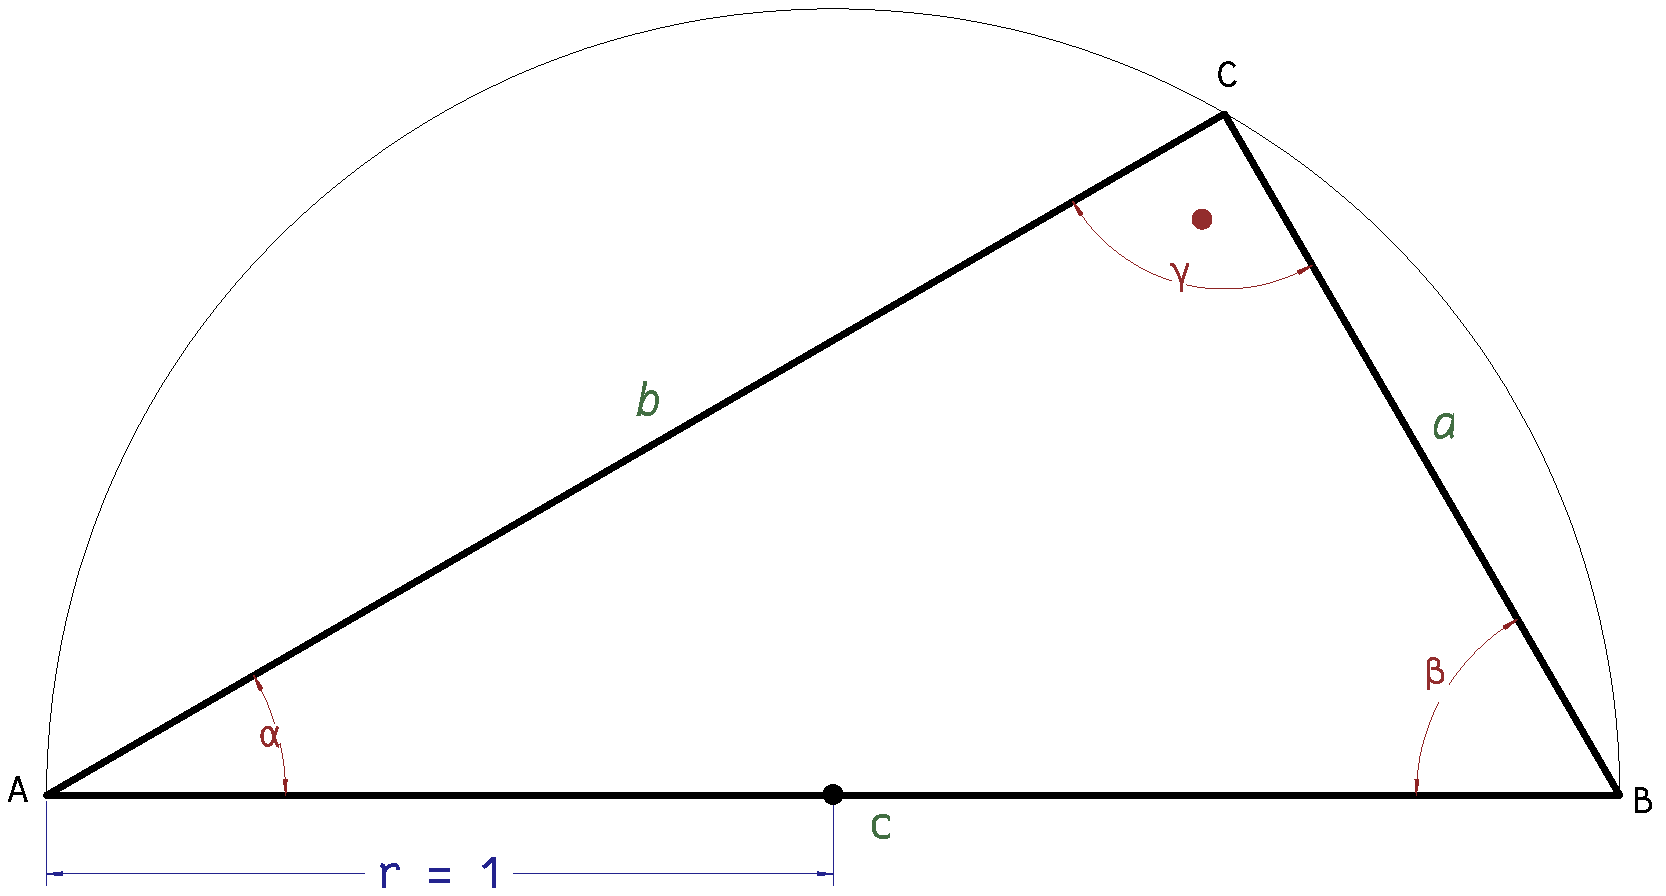
\includegraphics[width=0.5\textwidth]{Graphics/RightAngleTriangle}}\hfill
 \subfloat{\begin{tabular}{clc}
              \toprule
              Function              & Definition                            & Condition           \\
              \midrule
              sin(\skalar{\alpha})  & \skalar{a/c}                          & (\skalar{c \neq 0}) \\
              cos(\skalar{\alpha})  & \skalar{b/c}                          & (\skalar{c \neq 0}) \\
              tan(\skalar{\alpha})  & \skalar{a/b} = 1/cot(\skalar{\alpha}) & (\skalar{b \neq 0}) \\
              cot(\skalar{\alpha})  & \skalar{b/a} = 1/tan(\skalar{\alpha}) & (\skalar{a \neq 0}) \\
              sec(\skalar{\alpha})  & \skalar{c/b} = 1/cos(\skalar{\alpha}) & (\skalar{b \neq 0}) \\
              csc(\skalar{\alpha})  & \skalar{c/a} = 1/sin(\skalar{\alpha}) & (\skalar{a \neq 0}) \\
              \bottomrule
           \end{tabular} }
\end{figure}

For the sake of completeness, here some functions that are defined neither in standard Pascal, nor in the Lazarus \texttt{math} library:
\begin{lstlisting}[caption=Cyclometric functions]
  FUNCTION Sec(x: float): float;
    {Secans}

  VAR
    c: float;

  BEGIN
    c := Cos(x);
    IF c = 0
      THEN
        BEGIN
          CH := WriteErrorMessage('sec(x) with x = 90° or x = 270°');
          MathError := TRUE;
        END
      ELSE
        Result := 1 / c;
  END;


  FUNCTION Csc(x: float): float;

  VAR
    c: float;

  BEGIN
    c := Sin(x);
    IF c = 0
      THEN
        BEGIN
          CH := WriteErrorMessage('csc(x) with x = 90° or x = 270°');
          MathError := TRUE;
        END
      ELSE
        Result := 1 / c;
  END;

  FUNCTION ArcCot(x: float): float;

  BEGIN
    Result := Pi / 2 - ArcTan(x);
  END;


  FUNCTION ArcSec(x: float): float;

  BEGIN
    IF (x = 0) OR (Abs(x) > 1)
      THEN
        BEGIN
          CH := WriteErrorMessage('arcsec(x) with x not from [-1..1] or x = 0');
          MathError := TRUE;
        END
      ELSE
        Result := ArcCos(1 / x);
  END;


  FUNCTION ArcCsc(x: float): float;

  BEGIN
    IF (x = 0) OR (Abs(x) > 1)
      THEN
        BEGIN
          CH := WriteErrorMessage('arccsc(x) with x not from [-1..1] or x = 0');
          MathError := TRUE;
        END
      ELSE
        Result := ArcSin(1 / x);
  END;
\end{lstlisting}

\section{Routines required for statistics}

Even rather small numbers have large faculties, that can cause number overflows. The use of logarithms  avoids that problem:
\begin{lstlisting}[caption=logarithm of important functions]
  FUNCTION LnGamma(x: float): float;

  CONST
    a0 = 0.083333333096;
    a1 = -0.002777655457;
    a2 = 0.000777830670;
    c = 0.918938533205;

  VAR
    r: float;

  BEGIN
    r := (a0 + (a1 + a2 / Sqr(x)) / Sqr(x)) / x;
    Result := (x - 0.5) * Ln(x) - x + c + r;
  END;


  FUNCTION LnFak(x: float): float;

  VAR
    z: float;

  BEGIN
    z := x + 1;
    Result := LnGamma(z);
  END;
\end{lstlisting}

\begin{lstlisting}[caption=faculties (iterative)]
  FUNCTION fak(i: BYTE): LONGINT;

  VAR
    j: BYTE;
    Product: LONGINT;

  BEGIN
    Product := 1;    { fak(0) und fak(1) }
    FOR j := 2 TO i DO
      Product := Product * j;
    Result := Product;
  END;
\end{lstlisting}

The incomplete \( \gamma \)-function is calculated according to \parencite[p. 182]{Pre-89}, using either a series representation that converges quickly for \(x < a+1 \), or a continued fraction representation that converges quickly for \(x > a+1 \).

\subsection{Incomplete gamma-function}

\begin{lstlisting}[caption=Incomplete gamma function]
  FUNCTION IncompleteGamma(a, x: float): float;

  VAR
    GamSer, GamCF, gln: float;

    PROCEDURE GSer(a, x: float; VAR GamSer, gln: float);
    { series representation of incomplete gamma function, returns gamma in GamSer,
      ln(gamma) in gln. Converges quickly for x < succ(a) }

    VAR
      n: WORD;
      Sum, del, ap: float;

    BEGIN
      gln := LnGamma(a);
      IF (x <= 0)
        THEN
          BEGIN
            IF (x < 0)
              THEN
                BEGIN
                  ch := WriteErrorMessage('Error: Incomplete gamma-function: x < 0');
                  EXIT;
                END;
            GamSer := 0;
          END
        ELSE
          BEGIN
            ap := a;
            Sum := 1 / a;
            del := Sum;
            FOR n := 1 TO MaxIter DO
              BEGIN
                ap := ap + 1;
                del := del * x / ap;
                Sum := Sum + del;
                IF (Abs(del) < Abs(Sum) * MaxError)
                  THEN
                    BEGIN
                      ch := WriteErrorMessage(
                           'Error in incomplete gamma-function: no convergence ');
                      MathError := TRUE;
                      EXIT;
                    END;
              END;
            GamSer := Sum * Exp(-x + a * Ln(x) - gln);
          END;
    END;

    PROCEDURE gcf(a, x: float; VAR GamCF, gln: float);
    { continued fraction representation of incomplete gamma function, returns
      gamma in GamSer, ln(gamma) in gln. Converges quickly for x > succ(a) }

    VAR
      n: WORD;
      gOld, g, fac, b1, b0, anf, ana, an, a1, a0: float;

    BEGIN
      gln := LnGamma(a);
      gOld := 0.0;
      a0 := 1.0;
      a1 := x;
      b0 := 0.0;
      b1 := 1.0;
      fac := 1.0;
      FOR n := 1 TO MaxIter DO
        BEGIN
          an := 1.0 * n;
          ana := an - a;
          a0 := (a1 + a0 * ana) * fac;
          b0 := (b1 + b0 * ana) * fac;
          anf := an * fac;
          a1 := x * a0 + anf * a1;
          b1 := x * b0 + anf * b1;
          IF (a1 <> 0.0)
            THEN // renormalise
              BEGIN
                fac := 1.0 / a1;
                g := b1 * fac;
                IF (Abs((g - gOld) / g) < MaxError)
                  THEN  // convergence reached
                    BEGIN
                      GamCF := Exp(-x + a * Ln(x) - gln) * g;
                      EXIT;
                    END;
                gOld := g;
              END;
        END; // FOR
      ch := WriteErrorMessage('Error in incomplete gamma-function: no convergence');
      MathError := TRUE
    END;

  BEGIN
    IF (x < 0) OR (a <= 0)
      THEN
        BEGIN
          ch := WriteErrorMessage('Incomplete Gamma-function: arguments <= 0');
          MathError := TRUE;
          EXIT;
        END;
    IF (x < (a + 1.0))
      THEN
        BEGIN
          GSer(a, x, GamSer, gln);
          Result := 1.0 - GamSer;
        END
      ELSE
        BEGIN
          gcf(a, x, GamCF, gln);
          Result := GamCF;
        END;
  END;
\end{lstlisting}

\subsection{Binomial coefficients}

The binomial coefficient is the number of ways, in which \skalar{k} items can be chosen out of a set of \skalar{n}.
\begin{equation}
  \binom{n}{k} = \frac{n!}{k! (n-k)!} = \prod_{i=1}^k\frac{n + 1 -i}{i}
\end{equation}
The latter expression switches between multiplication and division, and hence avoids large numbers as much as possible. However, binomial coefficients -- even of relatively small numbers -- can be quite large, hence we use the float data type to avoid overflow.

\begin{lstlisting}[caption=binomial coefficient]
  FUNCTION BinomialCoef(n, k: LONGINT): float;

  VAR i,n1 : LONGINT;
    Res    : float;

  BEGIN
    IF n < k                // check FOR trivial cases first
      THEN Result := 0
      ELSE IF (n = k) OR (k = 0)
             THEN Result := 1
             ELSE IF k = 1
                    THEN Result := n
                    ELSE    // DO the real work
                      BEGIN
                        IF (2*k) > n THEN k := n-k;
                        Res := 1;
                        n1 := Succ(n);
                        FOR i := 1 TO k DO
                          Res := Res * (n1 - i) / i;
                        Result := Res;
                      END;
  END;
\end{lstlisting}


\section{Finance mathematics (with a German flavour)}

This routines converts a number into words

\begin{lstlisting}[caption=Finance mathematics]
  FUNCTION InWorten(Number: LONGINT): STRING;

  CONST
    Einer: ARRAY [1..9] OF STRING[6] =
      ('ein', 'zwei', 'drei', 'vier', 'fünf', 'sechs', 'sieben',
      'acht', 'neun');
    Zehner: ARRAY [1..9] OF STRING[8] =
      ('zehn', 'zwanzig', 'dreißig', 'vierzig', 'fünfzig',
      'sechzig', 'siebzig', 'achtzig', 'neunzig');
    Elfer: ARRAY [1..9] OF STRING[9] =
      ('elf', 'zwölf', 'dreizehn', 'vierzehn', 'fünfzehn', 'sechzehn',
      'siebzehn', 'achtzehn', 'neunzehn');

  VAR
    Minus: BOOLEAN;
    ZahlStr: STRING;
    ValueFeld: ARRAY [1..6] OF BYTE;

  BEGIN
    IF Number >= 1000000
      THEN
        BEGIN
          InWorten := ('Ungültiger Bereich ');
          EXIT;
        END;
    IF Number < 0
      THEN
        BEGIN
          Minus := TRUE;
          Number := Abs(Number);
        END
      ELSE
        Minus := FALSE;
    ValueFeld[1] := Number DIV 100000;    { Ziffern der Number isolieren }
    Number := Number MOD 100000;
    ValueFeld[2] := Number DIV 10000;
    Number := Number MOD 10000;
    ValueFeld[3] := Number DIV 1000;
    Number := Number MOD 1000;
    ValueFeld[4] := Number DIV 100;
    Number := Number MOD 100;
    ValueFeld[5] := Number DIV 10;
    ValueFeld[6] := Number MOD 10;
    ZahlStr := '';                     { String aufbauen, dabei die Besonderheiten }
    IF ValueFeld[1] > 0
      THEN ZahlStr := ZahlStr + Einer[ValueFeld[1]] + 'hundert';
    CASE ValueFeld[2] OF
      2..9: BEGIN
              IF ValueFeld[3] = 0
                THEN ZahlStr := ZahlStr + Zehner[ValueFeld[2]] + 'tausend'
                ELSE ZahlStr := ZahlStr + Einer[ValueFeld[3]] + 'und' +
                     Zehner[ValueFeld[2]] + 'tausend';
            END;
      1:    BEGIN
              IF ValueFeld[3] = 0
                THEN ZahlStr := ZahlStr + 'zehntausend'
                ELSE ZahlStr := ZahlStr + Elfer[ValueFeld[3]] + 'tausend';
            END;
      0:    BEGIN
              IF ValueFeld[3] = 0
                THEN
                  IF ZahlStr <> ''
                    THEN ZahlStr := ZahlStr + 'tausend'
                    ELSE
                ELSE
                  ZahlStr := ZahlStr + Einer[ValueFeld[3]] + 'tausend';
            END;
    END; // CASE
    IF ValueFeld[4] > 0
      THEN ZahlStr := ZahlStr + Einer[ValueFeld[4]] + 'hundert';
    CASE ValueFeld[5] OF
      2..9: BEGIN
              IF ValueFeld[6] = 0
                THEN ZahlStr := ZahlStr + Zehner[ValueFeld[5]]
                ELSE ZahlStr := ZahlStr + Einer[ValueFeld[6]] + 'und' + Zehner[ValueFeld[5]];
            END;
      1:    BEGIN
              IF ValueFeld[6] = 0
                THEN ZahlStr := ZahlStr + 'zehn'
                ELSE ZahlStr := ZahlStr + Elfer[ValueFeld[6]];
            END;
      0:    BEGIN
        CASE ValueFeld[6] OF
          0   : IF ZahlStr = '' THEN ZahlStr := 'null';
          1   : ZahlStr := ZahlStr + 'eins';
          2..9: ZahlStr := ZahlStr + Einer[ValueFeld[6]];
        END;
      END;
    END;
    ZahlStr[1] := UpCase(ZahlStr[1]);
    IF Minus THEN ZahlStr := 'minus ' + ZahlStr;
    Result := ZahlStr;
  END;
\end{lstlisting}

The modulo-11 number (a figure in 0..9 or the letter "X") is used for example to check the correctness of credit card numbers \parencite{Mic-96}.


\begin{lstlisting}[caption=test number by modulo-11 method]
  FUNCTION Modulo11(Number: LONGINT): CHAR;

  CONST
    ResultArr: ARRAY[0..10] OF CHAR =
      ('0', '1', '2', '3', '4', '5', '6', '7', '8', '9', 'X');

  VAR
    i, j, Sum: LONGINT;

  BEGIN
    i := 1;
    Number := Abs(Number);
    Sum := 0;
    WHILE Number > 0 DO
      BEGIN
        j := Number MOD 10;
        Number := Number DIV 10;
        Sum := Sum + i * j;
        i := i * 2;
      END;
    j := Sum MOD 11;
    Result := ResultArr[j];
  END;


  FUNCTION TestModulo11(Number: LONGINT; TEST: CHAR): BOOLEAN;

  BEGIN
    TestModulo11 := (Modulo11(Number) = TEST);
  END;
\end{lstlisting}

\section{Functions already in unit \texttt{math}}

Lazarus comes with the \texttt{math} unit, which contains many mathematical functions. In other compilers, these have to be replaced by own code. Then the following lines have to be added to the interface of \texttt{MathFunc}:
\begin{lstlisting}[caption=]
  function ArSinh (x: float): float;

  function ArCosh (x: float): float;

  function ArTanh (x: float): float;

  function sinh (x: float): float;

  function cosh (x: float): float;

  function tanh (x: float): float;

  function tan (x: float): float;

  function cotan (x: float): float;

  function ArcSin (x: float): float;

  function ArcCos (x: float): float;

  function ArcTan2 (x, y : float) : float;

  function log (x, Basis : float) : float;
\end{lstlisting}

and the following lines to the implementation:

\begin{lstlisting}[caption=]
  function ArSinh (x: float): float;

  begin
    Result := Ln(x + Sqrt(Sqr(x) + 1));
  end;


  function ArCosh (x: float): float;

  begin
    if x < 1.0
      then
        begin
          ch := WriteErrorMessage('Power of Base < 0 and broken exponent');
          MathError := true;
        end
      else
        Result := Ln(x + Sqrt(Sqr(x) - 1));
  end;


  function ArTanh (x: float): float;

  begin
    if abs(x) < 1.0
      then
        Result := 0.5 * Ln((1 + x) / (1 - x))
      else
        begin
          ch := WriteErrorMessage('artanh(x) with x not from [-1..1]');
          MathError := true;
          exit;
        end;
  end;

  function sinh (x: float): float;

  begin
    x := exp(x);
    Result := 0.5 * (x - 1 / x);
  end;


  function cosh (x: float): float;

  begin
    x := exp(x);
    Result := 0.5 * (x + 1 / x);
  end;


  function tanh (x: float): float;

  begin
    Result := sinh(x) / cosh(x);
  end;


  function tan (x: float): float;

  begin
    if Cos(x) <> 0
      then
        Result := Sin(x) / (Cos(x))
      else
        begin
          ch := WriteErrorMessage('tan(x) with x = 90° or x = 270°');
          MathError := true;
        end;
  end;


  function ArcSin (x: float): float;

  begin
    if abs(x) > 1.0
      then
        begin
          ch := WriteErrorMessage('arcsin(x) with x not from [-1..1]');
          MathError := true;
        end
      else
        if abs(x) < 1.0
          then Result := ArcTan(x / Sqrt(1 - Sqr(x)))
          else Result := x * Pi / 2
  end;


  function ArcCos (x: float): float;

  begin
    if abs(x) > 1.0
      then
        begin
          ch := WriteErrorMessage('arccos(x) with x not from [-1..1]');
          MathError := true;
        end
      else
         Result := Pi / 2 - ArcSin(x);
  end;


  function cotan (x: float): float;

  VAR tmp: float;

  begin
    tmp := Int(2 * x / Pi);
    if (tmp * Pi / 2) <> x
      then
        Result := 1 / tan(x)
      else
        begin
          ch := WriteErrorMessage('cot(x) with x not from [0..pi]');
          MathError := true;
        end;
  end;


  function arctan2 (x, y : float) : float;

  begin
    if x > 0
      then
        Result := arctan(y/x)
      else
        if x < 0
          then Result := arctan(y/x) + pi
          else Result := pi/2 * signum(y);
  end;
\end{lstlisting}

\printbibliography[heading=subbibliography]
\end{refsection}

  \chapter{Complex numbers}
\begin{refsection}

\abstract{Under standard Pascal, functions could only return simple data types. Complex numbers are -- in essence -- a record. However, Object Pascal allows such compound data types to be returned by functions.}

 The routines are based on \parencite{Gie-87,Thi-89}. The interface is:

\begin{lstlisting}[caption=Interface of \texttt{Complex}]
  UNIT Complex;

  INTERFACE

  USES Math, mathfunc;

  TYPE
    ComplexTyp = RECORD
      RealPart,
      ImagPart: float;
    END;

  CONST Const_i    : ComplexTyp = (RealPart : 0.0; ImagPart : 1.0);
        Const_Null : ComplexTyp = (RealPart : 0.0; ImagPart : 0.0);

  VAR
    ComplexError: BOOLEAN = FALSE;     // error-Flag

  { ************************ Type conversion **************************** }

  FUNCTION ComplexInit(RePart, ImPart: float): ComplexTyp;

  FUNCTION Re(z: ComplexTyp): float;
  { real part of a ComplexTyp number }

  FUNCTION Im(z: ComplexTyp): float;
  { imaginary part of a ComplexTyp number }

  { *************************** E/A- Routines *************************** }

  FUNCTION ComplexToStr(z: ComplexTyp; m, n: BYTE): STRING;

  { ***************************** Conversions *************************** }

  FUNCTION ComplexIsNull(z: ComplexTyp): BOOLEAN;

  FUNCTION ComplexConj(z: ComplexTyp): ComplexTyp;

  FUNCTION ComplexAbs(z: ComplexTyp): float;

  FUNCTION ComplexArg(z: ComplexTyp): float;

  FUNCTION ComplexInv(z: ComplexTyp): ComplexTyp;

  FUNCTION ComplexNeg(z: ComplexTyp): ComplexTyp;

  PROCEDURE Polar(z: ComplexTyp; VAR r, phi: float);

  FUNCTION Rect(r, phi: float): ComplexTyp;

  { ***************** Calculation with ComplexTyp ************** }

   OPERATOR = (z, b: ComplexTyp) : BOOLEAN;

   OPERATOR + (z, b: ComplexTyp): ComplexTyp;

   OPERATOR - (z, b: ComplexTyp): ComplexTyp;

   OPERATOR - (z: ComplexTyp): ComplexTyp;   // unary -

   OPERATOR * (z, b: ComplexTyp): ComplexTyp;

   OPERATOR / (z, b: ComplexTyp): ComplexTyp;

   OPERATOR ** (Basis, Exponent: ComplexTyp): ComplexTyp;

   { *********** Calculation with ComplexTyp and Real *********** }

   OPERATOR = (z: ComplexTyp; x: float) : BOOLEAN;

   OPERATOR = (x: float; z: ComplexTyp) : BOOLEAN;

   OPERATOR := (x: real) : ComplexTyp;

   OPERATOR := (z: ComplexTyp) : real;

   OPERATOR + (z: ComplexTyp; x: float) : ComplexTyp;

   OPERATOR + (x: float; z: ComplexTyp) : ComplexTyp;

   OPERATOR - (z : ComplexTyp; r : real) : ComplexTyp;

   OPERATOR - (r : real; z : ComplexTyp) : ComplexTyp;

   OPERATOR * (z: ComplexTyp; x: float): ComplexTyp;

   OPERATOR * (x: float; z: ComplexTyp) : ComplexTyp;

   OPERATOR / (z: ComplexTyp; x: float): ComplexTyp;

   OPERATOR / (x: float; z: ComplexTyp) : ComplexTyp;

   OPERATOR ** (Basis : ComplexTyp; Exponent : float) : ComplexTyp;

   OPERATOR ** (Basis : float; Exponent : ComplexTyp) : ComplexTyp;

  { ********************** Powers, roots ****************************** }

  FUNCTION ComplexLn(z: ComplexTyp): ComplexTyp;
  { ln(z) = ln(abs(z)) + i * arg(z) }

  FUNCTION ComplexExp(z: ComplexTyp): ComplexTyp;
  { exp(x + iy) = exp(x)*cos(y) + i*exp(x)*sin(y) }

  FUNCTION ComplexPower(Basis, Exponent: ComplexTyp): ComplexTyp;
  { b^e = exp(e * ln(b)) }

  FUNCTION ComplexPower(Basis: ComplexTyp; Exponent: float): ComplexTyp;
  { z^x = exp(x * ln(z)) }

  FUNCTION ComplexPower(Basis: float; Exponent: ComplexTyp): ComplexTyp;
  { x^z = exp(z * ln(x)) }

  FUNCTION ComplexRoot(z, b: ComplexTyp): ComplexTyp;
  { b-te Wurzel aus z = z^(1/b) }

  FUNCTION ComplexRoot(z: ComplexTyp; x: float): ComplexTyp;
  { x-te Wurzel aus z = z^(1/x) }

  FUNCTION ComplexRoot(x: float; z: ComplexTyp): ComplexTyp;
  { z-te Wurzel aus x = x^(1/z) }

  { *********************** Cyclometric functions ************************** }

  FUNCTION ComplexSin(z: ComplexTyp): ComplexTyp;
  { sin(x +- iy) = sin(x) * cosh(y) +- i * cos(x) * sinh(y) }

  FUNCTION ComplexCos(z: ComplexTyp): ComplexTyp;
  { cos(x +- iy) = cos(x) * cosh(y) +- i * sin(x) * sinh(y) }

  FUNCTION ComplexTan(z: ComplexTyp): ComplexTyp;
  { tan(x +- iy) = (sin(2x) / (cos(2x) + cosh(2x)) +- i * (sinh(2x) / (cos(2x) + cosh(2x)) }

  FUNCTION ComplexCot(z: ComplexTyp): ComplexTyp;
  { cot(z) = cos(z) / sin(z) }

  FUNCTION ComplexArcSin(z: ComplexTyp): ComplexTyp;
  { arcsin(z) = 1/i * ln(i*z + sqrt(1 - sqr(z))) }

  FUNCTION ComplexArcCos(z: ComplexTyp): ComplexTyp;
  { arccos(z) = 1/i * ln(z + sqrt(sqr(z) - 1)) }

  FUNCTION ComplexArcTan(z: ComplexTyp): ComplexTyp;
  { arctan(z) = 1/2i * ln((1+iz) / (1-iz)) }

  FUNCTION ComplexArcCot(z: ComplexTyp): ComplexTyp;
  { arccot(z) = -1/2i * ln((1+iz) / (iz - 1)) }

  { *********************** Hyperbolic funktions ********************** }

  FUNCTION ComplexSinh(z: ComplexTyp): ComplexTyp;
  { sinh(x + iy) = sinh(x)*cos(y) +- i*cosh(x)*sin(y)
                 = (exp(z) - exp(-z)) / 2 }

  FUNCTION ComplexCosh(z: ComplexTyp): ComplexTyp;
  { cosh(x + iy) = cosh(x)*cos(y) +- i*sinh(x)*sin(y)
                 = (exp(z) + exp(-z)) / 2 }

  FUNCTION ComplexTanh(z: ComplexTyp): ComplexTyp;
  { tanh(x + iy) = (sinh(2x)/(cosh(2x)+cos(2y)) + i*(sin(2y)/(cosh(2x)+cos(2y)))
                 = (exp(z) - exp(-z)) / (exp(z) + exp(-z)) }

  FUNCTION ComplexCoth(z: ComplexTyp): ComplexTyp;
  { coth(z) = cosh(z) / sinh(z) }

  FUNCTION ComplexArSinh(z: ComplexTyp): ComplexTyp;
  { arsinh(z) = ln(z + sqrt(sqr(z) + 1)) }

  FUNCTION ComplexArCosh(z: ComplexTyp): ComplexTyp;
  { arcosh(z) = ln(z + sqrt(sqr(z) - 1)) }

  FUNCTION ComplexArTanh(z: ComplexTyp): ComplexTyp;
  { artanh(z) := -1/2 * ln((1 + z) / (1 - z)) }

  FUNCTION ComplexArCoth(z: ComplexTyp): ComplexTyp;
  { arcoth(z) := 1/2 * ln((1 + z) / (z - 1)) }

  { *************************** Implementation ****************************** }

  IMPLEMENTATION

  VAR ch : CHAR;  // used for error handling
\end{lstlisting}

\section{Basic conversion and I/O routines}

\begin{lstlisting}[caption=Conversion and I/O routines]
  FUNCTION ComplexInit(RePart, ImPart: float): ComplexTyp;

  BEGIN
    Result.RealPart := RePart;
    Result.ImagPart := ImPart;
  END;


  FUNCTION Re(z: ComplexTyp): float;

  BEGIN
    Result := z.RealPart;
  END;


  FUNCTION Im(z: ComplexTyp): float;

  BEGIN
    Result := z.ImagPart;
  END;


  FUNCTION ComplexIsNull(z: ComplexTyp): BOOLEAN;

  BEGIN
    Result := (Abs(Re(z)) < Zero) AND (Abs(Im(z)) < Zero);
  END;


  FUNCTION ComplexToStr(z: ComplexTyp; m, n: BYTE): STRING;
    {Komplexe Zahl ausgeben}

  VAR
    OutStr, ImagStr: STRING;
    k: INTEGER;

  BEGIN
    Str(Re(z): m: n, OutStr);
    WHILE OutStr[1] = ' ' DO
      Delete(OutStr, 1, 1);
    IF Im(z) >= 0
      THEN OutStr := OutStr + '+'
      ELSE OutStr := OutStr + '-';
    Str(Abs(Im(z)): m: n, ImagStr);
    WHILE ImagStr[1] = ' ' DO
      Delete(ImagStr, 1, 1);
    OutStr := OutStr + ImagStr + 'i';
    FOR k := 1 TO (m - Length(OutStr)) DO
      OutStr := ' ' + OutStr;
    Result := OutStr;
  END;
\end{lstlisting}

The complex conjugate of a complex number \(z = x + \imath y \) is \(z^* = x - \imath y \):

\begin{lstlisting}
  FUNCTION ComplexConj(z: ComplexTyp): ComplexTyp;

  BEGIN
    Result := ComplexInit(Re(z), -Im(z));
  END;
\end{lstlisting}

The absolute value of a complex number is \(|z| = |x + \imath y| = \sqrt{x^2 + y^2} = \sqrt{z \times z^*} \):

\begin{lstlisting}
  FUNCTION ComplexAbs(z: ComplexTyp): float;

  VAR
    x: float;

  BEGIN
    x := (Sqr(Re(z)) + Sqr(Im(z)));
    IF Abs(x) < Zero
      THEN Result := 0
      ELSE Result := Sqrt(x);
  END;
\end{lstlisting}


\begin{lstlisting}
  FUNCTION ComplexArg(z: ComplexTyp): float;

  VAR
    i, r: float;

  BEGIN
    IF ComplexIsNull(z)
      THEN
        BEGIN
          ch := WriteErrorMessage(' Complex numbers: Argument of (0 + 0i)');
          ComplexError := TRUE;
          EXIT;
        END;
    i := Im(z);
    r := Re(z);
    IF r = 0
      THEN Result := Signum(i) * 0.5 * Pi
      ELSE
        IF r > 0
          THEN Result := ArcTan(i / r)
          ELSE Result := ArcTan(i / r) + Signum(i) * Pi;
  END;
\end{lstlisting}

\begin{lstlisting}
  FUNCTION ComplexInv (z : ComplexTyp) : ComplexTyp;

  BEGIN
    IF ComplexIsNull(z)
      THEN
        BEGIN
          ch := WriteErrorMessage('Complex Numbers: Attempt to invert (0 + 0i) ');
          ComplexError := TRUE;
        END
      ELSE Result := ComplexConj(z) / Sqr(ComplexAbs(z));
  END;
\end{lstlisting}


\begin{lstlisting}
  FUNCTION ComplexNeg(z: ComplexTyp): ComplexTyp;

  BEGIN
    Result := ComplexInit(-Re(z), -Im(z));
  END;
\end{lstlisting}


\begin{lstlisting}
  PROCEDURE Polar(z: ComplexTyp; VAR r, phi: float);

  BEGIN
    r := ComplexAbs(z);
    IF r <> 0
      THEN IF Abs(Im(z) / r) = 1
             THEN phi := Pi / 2 * (Im(z) / r) / Abs(Im(z) / r)
             ELSE phi := ArcTan(Im(z) / Re(z))
      ELSE
        BEGIN
          phi := 0;
          IF Re(z) < 0
            THEN
              IF Im(z) <> 0
                THEN phi := phi + Pi * Abs(Im(z)) / Im(z)
                ELSE phi := Pi;
        END;
  END;
\end{lstlisting}

\begin{lstlisting}
  FUNCTION Rect(r, phi: float): ComplexTyp;

  BEGIN
    Result := ComplexInit(r * Cos(phi), r * Sin(phi));
  END;
\end{lstlisting}


\section{Basic operators}

\subsection{Operators on complex variables}

In the following routines, we use operator overloading to assign meaning to the operators \( =, :=, +, -, *, /, ** \) for complex arguments \parencite{Can-20}.

Two complex numbers are equal if both their real and imaginary parts are equal:
\begin{lstlisting}
  OPERATOR = (z, b: ComplexTyp) : BOOLEAN;

  BEGIN
    Result := (Re(z) = Re(b)) AND (Im(z) = Im(b));
  END;
\end{lstlisting}

Two numbers \(a, b \in \mathbb{C} \) are added \(a + b = x_a + y_a\imath + x_b + y_b \imath = (x_a + x_b) + (y_a + yb)\imath \):

\begin{lstlisting}
  OPERATOR + (z, b: ComplexTyp): ComplexTyp;

  BEGIN
    Result := ComplexInit(Re(z) + Re(b), Im(z) + Im(b));
  END;
\end{lstlisting}


Similarly, for subtraction \(a - b = x_a + y_a\imath - x_b + y_b \imath = (x_a - x_b) + (y_a - y_b)\imath \):
\begin{lstlisting}
  OPERATOR - (z, b: ComplexTyp): ComplexTyp;

  BEGIN
    Result := ComplexInit(Re(z) - Re(b), Im(z) - Im(b));
  END;
\end{lstlisting}

There is also the unary minus:
\begin{lstlisting}
  OPERATOR - (z: ComplexTyp): ComplexTyp;

  BEGIN
    Result := ComplexInit(-Re(z), -Im(z));
  END;
\end{lstlisting}


Multiplication of complex numbers \(a \times\ b = (x_a + y_a\imath) \times\ (x_b + y_b \imath) = (x_a x_b - y_a y_b) + (x_a y_b + x_b y_a)\imath \).
\begin{lstlisting}
  OPERATOR * (z, b: ComplexTyp): ComplexTyp;

  VAR
    r, i: float;

  BEGIN
    r := Re(z) * Re(b) - Im(z) * Im(b);
    i := Re(z) * Im(b) + Im(z) * Re(b);
    Result := ComplexInit(r, i);
  END;
\end{lstlisting}

Once the multiplication is defined, we can also define the division of a complex number by a complex number \(a/b = a b^* / |b|^2 \).

\begin{lstlisting}
  OPERATOR / (z, b: ComplexTyp): ComplexTyp;

  VAR r, i : float;

  BEGIN
    IF ComplexIsNull(b)
      THEN
        BEGIN
          ch := WriteErrorMessage('Complex numbers: Division by (0 + 0i) ');
          ComplexError := TRUE;
          EXIT;
        END;
    r := (Re(z) * Re(b) + Im(z) * Im(b)) / (Sqr(Re(b)) + Sqr(Im(b)));
    i := (Im(z) * Re(b) - Re(z) * Im(b)) / (Sqr(Re(b)) + Sqr(Im(b)));
    Result := ComplexInit(r, i);
  END;
\end{lstlisting}

And finally, we can define a power operator:
\begin{lstlisting}
  OPERATOR ** (Basis, Exponent: ComplexTyp): ComplexTyp;

  BEGIN
    IF ComplexIsNull(Basis)
      THEN Result := ComplexInit(0, 0)
      ELSE Result := ComplexExp(Exponent * ComplexLn(Basis));
  END;
\end{lstlisting}

\subsection{Operators on mixed complex and real variables}

Operations which are commutative need to be defined for both the real, complex and the complex, real case.


Comparison:
\begin{lstlisting}
  OPERATOR = (z: ComplexTyp; x: float) : BOOLEAN;

  BEGIN
    Result := (Abs(Im(z)) < Zero) AND (Re(z) = x);
  END;

  OPERATOR = (x: float; z: ComplexTyp) : BOOLEAN;

  BEGIN
    Result := (Abs(Im(z)) < Zero) AND (Re(z) = x);
  END;
\end{lstlisting}



\begin{lstlisting}
  OPERATOR := (x: real) : ComplexTyp;

  BEGIN
    Result := ComplexInit(x, 0);
  END;


  OPERATOR := (z: ComplexTyp) : real;

  BEGIN
    IF Abs(Im(z)) > Zero
      THEN
        BEGIN
          ch := WriteErrorMessage('Assignment of complex to real variable: Im(z) <> 0');
          ComplexError := TRUE;
        END
      ELSE
        Result := Re(z);
  END;
\end{lstlisting}

\begin{lstlisting}
  OPERATOR + (z: ComplexTyp; x: float) : ComplexTyp;

  BEGIN
    Result := ComplexInit(x + Re(z), Im(z));
  END;

  OPERATOR + (x: float; z: ComplexTyp) : ComplexTyp;

  BEGIN
    Result := ComplexInit(x + Re(z), Im(z));
  END;
\end{lstlisting}

\begin{lstlisting}
  OPERATOR - (z : ComplexTyp; r : real) : ComplexTyp;

  BEGIN
    Result := ComplexInit(Re(z) - r, Im(z));
  END;


  OPERATOR - (r : real; z : ComplexTyp) : ComplexTyp;

  BEGIN
    Result := ComplexInit(r - Re(z), -Im(z));
  END;
\end{lstlisting}

We can also define the multiplication of a complex number \(a \) and a real number \(b \) as \(a \times\ b = x_a + y_a\imath \times\ b = x_a b + y_a b \imath \).
\begin{lstlisting}
  OPERATOR * (z: ComplexTyp; x: float) : ComplexTyp;

  BEGIN
    Result := ComplexInit(Re(z) * x, Im(z) * x);
  END;


  OPERATOR * (x: float; z: ComplexTyp) : ComplexTyp;

  BEGIN
    Result := ComplexInit(Re(z) * x, Im(z) * x);
  END;
\end{lstlisting}

\begin{lstlisting}
  OPERATOR / (z: ComplexTyp; x: float): ComplexTyp;

  BEGIN
    IF x = 0
      THEN
        BEGIN
          ch := WriteErrorMessage('Complex numbers: Attempt to divide by zero');
          ComplexError := TRUE;
        END
      ELSE
        Result := ComplexInit(Re(z) / x, Im(z) / x);
  END;


  OPERATOR / (x: float; z: ComplexTyp) : ComplexTyp;

  VAR d : float;

  BEGIN
    IF ComplexIsNull(z)
      THEN
        BEGIN
          ch := WriteErrorMessage('Complex numbers: Division by (0 + 0i) ');
          ComplexError := TRUE;
        END
      ELSE
        BEGIN
          d := Sqr(Re(z)) + Sqr(Im(z));
          Result := ComplexInit(x*Re(z)/d, -x*Im(z)/d);
        END;
  END;
\end{lstlisting}

\begin{lstlisting}
  OPERATOR ** (Basis : ComplexTyp; Exponent : float) : ComplexTyp;

  BEGIN
    IF ComplexIsNull(Basis)
      THEN Result := ComplexInit(0, 0)
      ELSE Result := ComplexExp(ComplexLn(Basis) * Exponent);
  END;


  OPERATOR ** (Basis : float; Exponent : ComplexTyp) : ComplexTyp;

  BEGIN
    IF Abs(Basis) < Zero
      THEN
        BEGIN
          ch := WriteErrorMessage('Complex numbers: Complex power of 0');
          ComplexError := TRUE;
        END
      ELSE
        Result := ComplexExp(Exponent * Ln(Basis));
  END;
\end{lstlisting}


\section{Logarithms and powers}

\(\exp(x + \imath y) = \exp(x)*\cos(y) + \imath \exp(x)*\sin(y) \). The logarithm of a complex number is \(\ln(z) = \ln(\abs(z)) + i * \arg(z) \)

\begin{lstlisting}[caption=Logarithm and exponential function]
  FUNCTION ComplexExp(z: ComplexTyp): ComplexTyp;

  VAR
    i, r: float;

  BEGIN
    i := Im(z);
    r := Exp(Re(z));
    Result := ComplexInit(r * Cos(i), r * Sin(i));
  END;


  FUNCTION ComplexLn(z: ComplexTyp): ComplexTyp;

  VAR r, i: float;

  BEGIN
    IF ComplexIsNull(z)
      THEN
        BEGIN
          ch := WriteErrorMessage('Complex numbers: Attempt to calculate ln(0+0i) ');
          ComplexError := TRUE;
        END
      ELSE
        BEGIN
          r := Ln(ComplexAbs(z));
          i := ComplexArg(z);
          Result := ComplexInit(r, i);
        END;
  END;
\end{lstlisting}

A base is raised to the power of an exponent by \(b^e = exp(e \times\ \ln(b)) \). This requires different function depending on whether \(b, z \in \mathbb{R} \) or \(\mathbb{C} \):

\begin{lstlisting}[caption=complex power function]
  FUNCTION ComplexPower(Basis, Exponent: ComplexTyp): ComplexTyp;

  BEGIN
    IF ComplexIsNull(Basis)
      THEN Result := ComplexInit(0, 0)
      ELSE Result := ComplexExp(Exponent * ComplexLn(Basis));
  END;


  FUNCTION ComplexPower(Basis: ComplexTyp; Exponent: float): ComplexTyp;

  BEGIN
    IF ComplexIsNull(Basis)
      THEN Result := ComplexInit(0, 0)
      ELSE Result := ComplexExp(ComplexLn(Basis) * Exponent);
  END;


  FUNCTION ComplexPower(Basis: float; Exponent: ComplexTyp): ComplexTyp;

  BEGIN
    IF Abs(Basis) < Zero
      THEN
        BEGIN
          ch := WriteErrorMessage('Complex numbers: Complex power of 0');
          ComplexError := TRUE;
        END
      ELSE
        Result := ComplexExp(Exponent * Ln(Basis));
  END;
\end{lstlisting}

The root of a number is calculated by \(\sqrt[b]{z} = z^{1/b} \). This requires different function depending on whether \(b, z \in \mathbb{R} \) or \(\mathbb{C} \):

\begin{lstlisting}
  FUNCTION ComplexRoot(z, b: ComplexTyp): ComplexTyp;

  BEGIN
    IF ComplexIsNull(b)
      THEN
        BEGIN
          ch := WriteErrorMessage('Complex numbers: Attempt to calculate the (0 + 0i)-th root');
          ComplexError := TRUE;
          EXIT;
        END
      ELSE
        Result := ComplexPower(z, ComplexInv(b));
  END;


  FUNCTION ComplexRoot(z: ComplexTyp; x: float): ComplexTyp;

  BEGIN
    IF x = 0
      THEN
        BEGIN
          ch := WriteErrorMessage('Complex numbers: 0-th root');
          ComplexError := TRUE;
        END
      ELSE
        IF ComplexIsNull(z)
          THEN Result := ComplexInit(0, 0)
          ELSE Result := ComplexPower(z, 1 / x);
  END;


  FUNCTION ComplexRoot(x: float; z: ComplexTyp): ComplexTyp;

  BEGIN
    IF ComplexIsNull(z)
      THEN
        BEGIN
          ch := WriteErrorMessage('Complex numbers: (0 + 0i)-th root');
          ComplexError := TRUE;
        END
      ELSE IF x = 0
             THEN Result := ComplexInit(0, 0)
             ELSE Result := ComplexPower(x, ComplexInv(z));
  END;
\end{lstlisting}

\section{Angle and cyclometric functions}

 \(sin(x \pm\ \imath y) = \sin(x) \times \cosh(y) \pm \imath \cos(x)  \sinh(y) \):

\begin{lstlisting}
  FUNCTION ComplexSin(z: ComplexTyp): ComplexTyp;

  VAR
    r, i: float;

  BEGIN
    r := Sin(Re(z)) * cosh(Im(z));
    i := Cos(Re(z)) * sinh(Im(z));
    Result := ComplexInit(r, i);
  END;
\end{lstlisting}

\(\cos(x \pm\ \imath y) = \cos(x) * \cosh(y) \pm\ \imath * \sin(x) * \sinh(y) \):

\begin{lstlisting}
  FUNCTION ComplexCos(z: ComplexTyp): ComplexTyp;

  VAR
    r, i: float;

  BEGIN
    r := Cos(Re(z)) * cosh(Im(z));
    i := -Sin(Re(z)) * sinh(Im(z));
    Result := ComplexInit(r, i);
  END;
\end{lstlisting}

\(\tan(x \pm\ \imath y) = \frac{\sin(2x)}{\cos(2x) + \cosh(2y)} \pm\ \imath \frac{\sinh(2y)}{\cos(2x) + \cosh(2y)} \):

\begin{lstlisting}
  FUNCTION ComplexTan(z: ComplexTyp): ComplexTyp;

  VAR
    r, i: float;

  BEGIN
    r := Sin(2 * Re(z)) / (Cos(2 * Re(z)) + cosh(2 * Im(z)));
    i := sinh(2 * Im(z)) / (Cos(2 * Re(z)) + cosh(2 * Im(z)));
    Result := ComplexInit(r, i);
  END;
\end{lstlisting}

\(\cot(z) = \frac{\cos(z)}{\sin(z)} \):

\begin{lstlisting}
  FUNCTION ComplexCot(z: ComplexTyp): ComplexTyp;

  BEGIN
    IF ComplexIsNull(z)
      THEN
        BEGIN
          ch := WriteErrorMessage('Complex numbers: Attempt to calculate cot(0 + 0i) ');
          ComplexError := TRUE;
        END
      ELSE
        Result := ComplexCos(z) / ComplexSin(z);
  END;
\end{lstlisting}

\( \arcsin(z) = 1/\imath \times \ln(\imath z + \sqrt{1 - z^2}) \):

\begin{lstlisting}
  FUNCTION ComplexArcSin(z: ComplexTyp): ComplexTyp;

  VAR
    c0, c1, c2, c3: ComplexTyp;

  BEGIN
    IF ComplexIsNull(z)
      THEN
        BEGIN
          ch := WriteErrorMessage('Complex Numbers: Attempt to calculate arcsin(0 + 0i) ');
          ComplexError := TRUE;
          EXIT;
        END;
    c1 := ComplexInit(1, 0);
    c2 := ComplexInit(0, 1);
    c3 := ComplexInit(0, -1);
    c0 := ComplexRoot(c1 - ComplexPower(z, 2), 2);
    c0 := ComplexLn(c2 * z + c0);
    Result := c3 * c0;
  END;
\end{lstlisting}

\(\arccos(z) = 1/\imath \times \ln(z + \sqrt{z^2 - 1}) \):

\begin{lstlisting}
  FUNCTION ComplexArcCos(z: ComplexTyp): ComplexTyp;

  VAR
    c0, c1, c2: ComplexTyp;

  BEGIN
    IF ComplexIsNull(z)
      THEN
        BEGIN
          ch := WriteErrorMessage('Complex numbers: Attempt to calculate arccos(0 + 0i) ');
          ComplexError := TRUE;
          EXIT;
        END;
    c1 := ComplexInit(1.0, 0.0);
    c2 := ComplexInit(0.0, -1.0);
    c0 := ComplexRoot(ComplexPower(z, 2) - c1, 2);
    Result := ComplexLn(z + c0) * c2;
  END;
\end{lstlisting}

\( \arctan(z) = \frac{1}{2} \imath \times \ln(\frac{1 + \imath z}{1 - \imath z}) \):

\begin{lstlisting}
  FUNCTION ComplexArcTan(z: ComplexTyp): ComplexTyp;

  VAR
    c0, c1, c2, c3, a1, a2: ComplexTyp;

  BEGIN
    IF ComplexIsNull(z)
      THEN
        BEGIN
          ch := WriteErrorMessage('Complex numbers: Attempt to calculate arctan(0 + 0i) ');
          ComplexError := TRUE;
          EXIT;
        END;
    c1 := ComplexInit(0, 1);
    c2 := ComplexInit(1, 0);
    c3 := ComplexInit(0, 2);
    c0 := c1 * z;
    a1 := c2 + c0;
    a2 := c2 - c0;
    c0 := ComplexLn(a1 / a2);
    a1 := c2 / c3;
    Result := a1 * c0;
  END;
\end{lstlisting}

\( \mathrm{arccot}(z) = -\frac{1}{2} \imath \times \ln(\frac{1 + \imath z}{\imath z - 1}) \):

\begin{lstlisting}
  FUNCTION ComplexArcCot(z: ComplexTyp): ComplexTyp;

  VAR
    c0, c1, c2, c3, a1, a2: ComplexTyp;

  BEGIN
    IF ComplexIsNull(z)
      THEN
        BEGIN
          ch := WriteErrorMessage('Complex numbers: Attempt to calculate arccot(0 + 0i) ');
          ComplexError := TRUE;
          EXIT;
        END;
    c1 := ComplexInit(0, 1);
    c2 := ComplexInit(1, 0);
    c3 := ComplexInit(0, -2);
    c0 := c1 * z;
    a1 := c0 + c2;
    a2 := c0 - c2;
    c0 := ComplexLn(a1 / a2);
    a1 := c2 / c3;
    Result := a1 * c0;
  END;
\end{lstlisting}


\section{Hyperbolic functions}

\( \sinh(x + \imath y) = \sinh(x) \cos(y) + \imath \cosh(x) \sin(y) = \frac{\exp(z) - \exp(-z)}{2} \):

\begin{lstlisting}
  FUNCTION ComplexSinh(z: ComplexTyp): ComplexTyp;

  VAR
    r, i: float;

  BEGIN
    r := sinh(Re(z)) * Cos(Im(z));
    i := cosh(Re(z)) * Sin(Im(z));
    Result := ComplexInit(r, i);
  END;
\end{lstlisting}

\( \cosh(x + \imath y) = \cosh(x) \cos(y) \pm\ \imath \sinh(x) \sin(y)  = \frac{\exp(z) + \exp(-z)}{2} \):

\begin{lstlisting}
  FUNCTION ComplexCosh(z: ComplexTyp): ComplexTyp;

  VAR
    r, i: float;

  BEGIN
    r := cosh(Re(z)) * Cos(Im(z));
    i := sinh(Re(z)) * Sin(Im(z));
    Result := ComplexInit(r, i);
  END;
\end{lstlisting}

\( \tanh(x + \imath y) = (\sinh(2 x)/(\cosh(2 x) + \cos(2 y)) + \imath (\sin(2 y)/(\cosh(2 x) + \cos(2 y)))  = \frac{\exp(z) - \exp(-z)}{\exp(z) + \exp(-z)} \):

\begin{lstlisting}
  FUNCTION ComplexTanh(z: ComplexTyp): ComplexTyp;

  VAR
    r, i: float;

  BEGIN
    r := sinh(2 * Re(z)) / (cosh(2 * Re(z)) + Cos(2 * Im(z)));
    i := Sin(2 * Im(z)) / (cosh(2 * Re(z)) + Cos(2 * Im(z)));
    Result := ComplexInit(r, i);
  END;
\end{lstlisting}

\( \coth(z) = \frac{\cosh(z)}{\sinh(z)} \):

\begin{lstlisting}
  FUNCTION ComplexCoth (z : ComplexTyp) : ComplexTyp;

  BEGIN
    IF ComplexIsNull(z)
      THEN
        BEGIN
          ch := WriteErrorMessage('Complex numbers: Attempt to calculate coth(0 + 0i) ');
          ComplexError := TRUE;
        END
      ELSE
        Result := ComplexCosh(z) / ComplexSinh(z);
  END;
\end{lstlisting}

\section{Area functions}

\( \mathrm{arsinh}(z) = \ln(z + \sqrt{z^2 + 1}) \):

\begin{lstlisting}
  FUNCTION ComplexArSinh(z: ComplexTyp): ComplexTyp;

  VAR
    c0, c1: ComplexTyp;

  BEGIN
    IF ComplexIsNull(z)
      THEN
        BEGIN
          ch := WriteErrorMessage('Complex numbers: Attempt to calculate arsinh(0 + 0i) ');
          ComplexError := TRUE;
        END
      ELSE
        BEGIN
          c1 := ComplexInit(1, 0);
          c0 := ComplexRoot(ComplexPower(z, 2) + c1, 2);
          Result := ComplexLn(z + c0);
        END;
  END;
\end{lstlisting}

\( \mathrm{arcosh}(z) = \ln(z + \sqrt{z^2 - 1}) \):

\begin{lstlisting}
  FUNCTION ComplexArCosh(z: ComplexTyp): ComplexTyp;

  VAR
    c0, c1: ComplexTyp;

  BEGIN
    IF ComplexIsNull(z)
      THEN
        BEGIN
          ch := WriteErrorMessage('Complex numbers: Attempt to calculate arcosh(0 + 0i) ');
          ComplexError := TRUE;
        END
      ELSE
        BEGIN
          c1 := ComplexInit(1, 0);
          c0 := ComplexRoot(ComplexPower(z, 2) - c1, 2);
          Result := ComplexLn(z + c0);
        END;
  END;
\end{lstlisting}

\( \mathrm{artanh}(z) := -\frac{1}{2} * \ln(\frac{1 + z}{1 - z}) \):

\begin{lstlisting}
  FUNCTION ComplexArTanh(z: ComplexTyp): ComplexTyp;

  VAR
    c0, c1, c2, a1, a2: ComplexTyp;

  BEGIN
    IF ComplexIsNull(z)
      THEN
        BEGIN
          ch := WriteErrorMessage('Complex numbers: Attempt to calculate artanh(0 + 0i) ');
          ComplexError := TRUE;
        END
      ELSE
        BEGIN
          c1 := ComplexInit(1, 0);
          c2 := ComplexInit(2, 0);
          a1 := c1 + z;
          a2 := c1 - z;
          c0 := ComplexLn(a1 / a2);
          Result := c0 / c2;
        END;
  END;
\end{lstlisting}

\( \mathrm{arcoth}(z) := \frac{1}{2} * \ln(\frac{1 + z}{z - 1}) \):

\begin{lstlisting}
  FUNCTION ComplexArCoth(z: ComplexTyp): ComplexTyp;

  VAR
    c0, c1, c2, a1, a2: ComplexTyp;

  BEGIN
    IF ComplexIsNull(z)
      THEN
        BEGIN
         ch := WriteErrorMessage('Complex numbers: Attempt to calculate arcoth(0 + 0i) ');
         ComplexError := TRUE;
        END
      ELSE
        BEGIN
          c1 := ComplexInit(1, 0);
          c2 := ComplexInit(2, 0);
          a1 := z + c1;
          a2 := z - c1;
          c0 := ComplexLn(a1 / a2);
          Result := c0 / c2;
        END;
  END;

  END. // UNIT Complex
\end{lstlisting}

\section{Test program}

A simple test program can be used to identify problems. It is based on applying the reciprocal function to the result of a function, this should return the original argument:

\begin{lstlisting}
  PROGRAM TestComplex;

  USES Mathfunc, Complex;

  VAR a, b, c, d : ComplexTyp;
      x, y, z    : double;


  PROCEDURE EinOperand(a, r : ComplexTyp; Operation : STRING);

  BEGIN
    Write(Operation,'(');
    Write(ComplexToStr(a, 6, 3));
    Write(') = ');
    Write(ComplexToStr(r, 6, 3));
    Writeln;
  END;


  PROCEDURE ZweiOperanden (a1, a2, r : ComplexTyp; Operation : STRING);

  BEGIN
    Write('(');
    Write(ComplexToStr(a1, 6, 3));
    Write(') ', Operation, ' (');
    Write(ComplexToStr(a2, 6, 3));
    Write(') = (');
    Write(ComplexToStr(r, 6, 3));
    Writeln(')');
  END;


  PROCEDURE ComplexMitReel (a1, r : ComplexTyp; a2 : double; Operation : STRING);

  BEGIN
    Write('(');
    Write(ComplexToStr(a1, 6, 3));
    Write(') ', Operation, ' ', a2:6:3);
    Write(' = (');
    Write(ComplexToStr(r, 6, 3));
    Writeln(')');
  END;


  PROCEDURE TestAddSub;

  BEGIN
    c := a + b;
    ZweiOperanden(a, b, c, '+');
    d := c - b;
    ZweiOperanden(c, b, d, '-');
  END;


  PROCEDURE TestMulDiv;

  BEGIN
    c := a * b;
    ZweiOperanden(a, b, c, '*');
    d := c / b;
    IF ComplexError
      THEN ComplexError := FALSE
      ELSE ZweiOperanden(c, b, d, '/');
  END;


  PROCEDURE TestMulDivMitReel;

  BEGIN
    b := a * x;
    ComplexMitReel(a, b, x, '*');
    c := b / x;
    IF ComplexError
      THEN ComplexError := FALSE
      ELSE ComplexMitReel(b, c, x, '/');
  END;


  PROCEDURE TestPolarRect;

  BEGIN
    Polar(a, y, z);
    c := Rect(y, z);
    Write('Polar(');
    Write(ComplexToStr(a, 6, 3));
    Writeln(') = (', y:6:3, ', ', z:6:3, ')');
    Write('Rect(', y:6:3, ', ', z:6:3, ') = (');
    Write(ComplexToStr(c, 6, 3));
    Writeln(')');
  END;


  PROCEDURE TestExpLn;

  BEGIN
    b := ComplexExp(a);
    IF ComplexError
      THEN
        BEGIN
          ComplexError := FALSE;
          EXIT;
        END;
    EinOperand(a, b, 'exp');
    c := ComplexLn(b);
    IF ComplexError
      THEN ComplexError := FALSE
      ELSE EinOperand(b, c, 'ln');
  END;


  PROCEDURE TestPotReelComplex;

  BEGIN
    b := ComplexPower(x, a);
    IF ComplexError
      THEN
        BEGIN
          ComplexError := FALSE;
          EXIT;
        END;
    Write(x:6:3, '^(');
    Write(ComplexToStr(a, 6, 3));
    Write(') = ');
    Write(ComplexToStr(b, 6, 3));
    Writeln;
    c := ComplexRoot(b, a);
    IF ComplexError
      THEN
        BEGIN
          ComplexError := FALSE;
          EXIT;
        END;
    Write('(');
    Write(ComplexToStr(b, 6, 3));
    Write(')^1/(');
    Write(ComplexToStr(a, 6, 3));
    Write(') = ');
    Write(ComplexToStr(c, 6, 3));
    Writeln;
  END;


  PROCEDURE TestPotComplexReel;

  BEGIN
    b := ComplexPower(a, x);
    IF ComplexError
      THEN
        BEGIN
          ComplexError := FALSE;
          EXIT;
        END;
    ComplexMitReel(a, b, x, '^');
    c := ComplexRoot(b, x);
    IF ComplexError
      THEN
        BEGIN
          ComplexError := FALSE;
          EXIT;
        END;
    ComplexMitReel(b, c, x, '^1/');
  END;


  PROCEDURE TestPotComplexComplex;

  BEGIN
    c := ComplexPower(a, b);
    IF ComplexError
      THEN
        BEGIN
          ComplexError := FALSE;
          EXIT;
        END;
    ZweiOperanden(a, b, c, '^');
    d := ComplexRoot(c, b);
    IF ComplexError
      THEN
        BEGIN
          ComplexError := FALSE;
          EXIT;
        END;
    ZweiOperanden(c, b, d, '^1/');
  END;


  PROCEDURE TestSin;

  BEGIN
    b := ComplexSin(a);
    IF ComplexError
      THEN
        BEGIN
          ComplexError := FALSE;
          EXIT;
        END;
    EinOperand(a, b, 'sin');
    c := ComplexArcSin(b);
    IF ComplexError
      THEN
        BEGIN
          ComplexError := FALSE;
          EXIT;
        END;
    EinOperand(b, c, 'arcsin');
  END;


  PROCEDURE TestCos;

  BEGIN
    b := ComplexCos(a);
    IF ComplexError
      THEN
        BEGIN
          ComplexError := FALSE;
          EXIT;
        END;
    EinOperand(a, b, 'cos');
    c := ComplexArcCos(b);
    IF ComplexError
      THEN
        BEGIN
          ComplexError := FALSE;
          EXIT;
        END;
    EinOperand(b, c, 'arccos');
  END;


  PROCEDURE TestTan;

  BEGIN
    b := ComplexTan(a);
    IF ComplexError
      THEN
        BEGIN
          ComplexError := FALSE;
          EXIT;
        END;
    EinOperand(a, b, 'tan');
    c := ComplexArcTan(b);
    IF ComplexError
      THEN
        BEGIN
          ComplexError := FALSE;
          EXIT;
        END;
    EinOperand(b, c, 'arctan');
  END;


  PROCEDURE TestCot;

  BEGIN
    b := ComplexCot(a);
    IF ComplexError
      THEN
        BEGIN
          ComplexError := FALSE;
          EXIT;
        END;
    EinOperand(a, b, 'cot');
    c := ComplexArcCot(b);
    IF ComplexError
      THEN
        BEGIN
          ComplexError := FALSE;
          EXIT;
        END;
    EinOperand(b, c, 'arctan');
  END;


  PROCEDURE TestSinh;

  BEGIN
    b := ComplexSinh(a);
    IF ComplexError
      THEN
        BEGIN
          ComplexError := FALSE;
          EXIT;
        END;
    EinOperand(a, b, 'sinh');
    c := ComplexArSinh(b);
    IF ComplexError
      THEN
        BEGIN
          ComplexError := FALSE;
          EXIT;
        END;
    EinOperand(b, c, 'arsinh');
  END;


  PROCEDURE TestCosh;

  BEGIN
    b := ComplexCosh(a);
    IF ComplexError
      THEN
        BEGIN
          ComplexError := FALSE;
          EXIT;
        END;
    EinOperand(a, b, 'cosh');
    c := ComplexArCosh(b);
    IF ComplexError
      THEN
        BEGIN
          ComplexError := FALSE;
          EXIT;
        END;
    EinOperand(b, c, 'arcosh');
  END;


  PROCEDURE TestTanh;

  BEGIN
    b := ComplexTanh(a);
    IF ComplexError
      THEN
        BEGIN
          ComplexError := FALSE;
          EXIT;
        END;
    EinOperand(a, b, 'tanh');
    c := ComplexArTanh(b);
    IF ComplexError
      THEN
        BEGIN
          ComplexError := FALSE;
          EXIT;
         END;
    EinOperand(b, c, 'artanh');
  END;


  PROCEDURE TestCoth;

  BEGIN
    b := ComplexCoth(a);
    IF ComplexError
      THEN
        BEGIN
          ComplexError := FALSE;
          EXIT;
        END;
    EinOperand(a, b, 'coth');
    c := ComplexArCoth(b);
    IF ComplexError
      THEN
        BEGIN
          ComplexError := FALSE;
          EXIT;
        END;
    EinOperand(b, c, 'arcoth');
  END;


  PROCEDURE TestAll;

  VAR c : ComplexTyp;

  BEGIN
    TestAddSub; Writeln;
    TestMulDiv; Writeln;
    TestMulDivMitReel; Writeln;
    TestPolarRect; Writeln;
    TestExpLn; Writeln;
    TestPotReelComplex; Writeln;
    TestPotComplexReel; Writeln;
    TestPotComplexComplex; Writeln;
    TestSin; Writeln;
    TestCos; Writeln;
    TestTan; Writeln;
    TestCot; Writeln;
    TestSinh; Writeln;
    TestCosh; Writeln;
    TestTanh; Writeln;
    TestCoth; Writeln;
    ReadLn;
  END;


  BEGIN
    a := ComplexInit(0.621, 0.567);
    b := ComplexInit(0.5, 0.4);
    x := 1.5;
    TestAll;
    a := ComplexInit(1.0, -1.0);
    x := 0.2;
    TestAll;
    a := ComplexInit(-0.5, 0.2);
    x := 0.2;
    TestAll;
    a := ComplexInit(-1.0, -1.5);
    x := 1.5;
    TestAll;
    a := ComplexInit(1.0, 0.0);
    x := 1.5;
    TestAll;
    a := ComplexInit(0.0, 1.0);
    x := 1.5;
    TestAll;
    a := ComplexInit(0.0, 0.0);
    x := 1.5;
    TestAll;
  END.
\end{lstlisting}


% Problem case
% (-1.0 - 1.5i)^1.5 = (-2.409 + 0.233i)
% (-2.409 + 0.233i)^1/1.5 = (-0.799 + 1.616i)
%
% (-1.0 - 1.5i)^(-2.409 + 0.233i) = (0.235 - 0.324i)
% (0.235 - 0.324i)^1/(-2.409 + 0.233i) = (1.279 + 0.579i)

\printbibliography[heading=subbibliography]
\end{refsection}


  \chapter{Big sets}
\begin{refsection}

\abstract{The set data type in pascal is limited to \texttt{MaxByte} (\num{255}) members. In some applications, this is insufficient. This unit defines a set type with arbitrary size and the operations that can be performed on it.}

A set is, in effect, an \texttt{array [0..pred(MaxCardinality)] of bit}. Each bit stands for one member, and is 1 if that member is in the set and 0 if it is not. However, there is no data type bit in Pascal, so we implement the array as an \texttt{array of word}. \texttt{MaxCardinality} should be a multiple of the \texttt{WordSize}, which is \SI{2}{byte} = \SI{16}{bit} under Lazarus for Windows. Thus, for our purposes, it is reasonable to set \texttt{MaxCardinality} = \num{2048}. Then we only need to define routines that allow access to individual bits. The interface of such a unit would be:
\begin{lstlisting}[caption=Interface]
  UNIT BigSet;

  INTERFACE

  USES Classes;

  CONST MaxCardinality = 2048;                                       // change AS needed
        WordSize       = SizeOf(WORD) * 8;                           // IN bits
        MaxMembers     = Pred(MaxCardinality DIV (WordSize));        // number OF words needed TO fit elements

  TYPE SetType = ARRAY [0..MaxMembers] OF WORD;

  PROCEDURE SetBit (VAR S : SetType; Bit : WORD);

  PROCEDURE ClearBit (VAR S : SetType; Bit : WORD);

  PROCEDURE ToggleBit (VAR S : SetType; Bit : WORD);

  PROCEDURE ClearAllBits (VAR S : SetType);

  PROCEDURE SetAllBits (VAR S : SetType);

  FUNCTION InSet (CONST S : SetType; Bit : WORD) : BOOLEAN;

  PROCEDURE SetUnion (VAR S: SetType; CONST T, U : SetType);

  PROCEDURE SetIntersection (VAR S: SetType; CONST T, U : SetType);

  PROCEDURE SetComplement (VAR S: SetType; CONST T, U : SetType);

  PROCEDURE SetSymDifference (VAR S: SetType; CONST T, U : SetType);

  FUNCTION SubSet (CONST S, T : SetType) : BOOLEAN;

  FUNCTION TrueSubSet (CONST S, T : SetType) : BOOLEAN;

  FUNCTION EqualSet (CONST S, T : SetType) : BOOLEAN;

  FUNCTION EmptySet (CONST S : SetType) : BOOLEAN;

FUNCTION Cardinality (CONST S : SetType) : WORD;
\end{lstlisting}

\begin{lstlisting}[caption=Implementation]
  IMPLEMENTATION

  CONST Bits : ARRAY [0..15] OF WORD = (   1,    2,    4,    8,   16,   32,    64,   128,
                                         256,  512, 1024, 2048, 4096, 8192, 16384, 32768);

  PROCEDURE SetBit(VAR S : SetType; Bit : WORD);

  VAR n : WORD;

  BEGIN
    n := Bit DIV WordSize;         // identify the WORD that stores the bit
    S[n] := S[n] OR Bits[Bit MOD 16];
  END;


  PROCEDURE ClearBit (VAR S : SetType; Bit : WORD);

  VAR n : WORD;

  BEGIN
    n := Bit DIV WordSize;
    S[n] := S[n] AND NOT Bits[Bit MOD 16];
  END;


  PROCEDURE ToggleBit (VAR S : SetType; Bit : WORD);

  VAR n : WORD;

  BEGIN
    n := Bit DIV WordSize;
    S[n] := S[n] XOR Bits[Bit MOD 16];
  END;


  FUNCTION InSet (CONST S : SetType; Bit : WORD) : BOOLEAN;

  VAR n : WORD;

  BEGIN
    n := Bit DIV WordSize;
    Result := S[n] AND Bits[Bit MOD 16] <> 0;
  END;

  PROCEDURE ClearAllBits (VAR S : SetType);

  VAR n : WORD;

  BEGIN
    FOR n := 0 TO MaxMembers DO
      S[n] := 0;
  END;

  PROCEDURE SetAllBits (VAR S : SetType);

  VAR n : WORD;

  BEGIN
    FOR n := 0 TO MaxMembers DO
      S[n] := Pred(MaxCardinality);
  END;

  PROCEDURE SetUnion (VAR S: SetType; CONST T, U : SetType);

  VAR n : WORD;
  BEGIN
    FOR n := 0 TO Pred(MaxCardinality) DO
      IF (InSet(T, n) OR InSet(U, n))
        THEN SetBit(S, n)
        ELSE ClearBit(S, n);
  END;

  PROCEDURE SetIntersection (VAR S: SetType; CONST T, U : SetType);

  VAR n : WORD;
  BEGIN
    FOR n := 0 TO Pred(MaxCardinality) DO
      IF (InSet(T, n) AND InSet(U, n))
        THEN SetBit(S, n)
        ELSE ClearBit(S, n);
  END;

  PROCEDURE SetComplement (VAR S: SetType; CONST T, U : SetType);

  VAR n : WORD;
  BEGIN
    FOR n := 0 TO Pred(MaxCardinality) DO
      IF (InSet(T, n) AND NOT(InSet(U, n)))
        THEN SetBit(S, n)
        ELSE ClearBit(S, n);
  END;

  PROCEDURE SetSymDifference (VAR S: SetType; CONST T, U : SetType);

  VAR H1, H2 : SetType;

  BEGIN
    SetComplement(H1, T, U);
    SetComplement(H2, U, T);
    SetUnion(S, H1, H2)
  END;

  FUNCTION SubSet (CONST S, T : SetType) : BOOLEAN;

  VAR n : WORD;
  BEGIN
    FOR n := 0 TO Pred(MaxCardinality) DO
      IF (InSet(S, n) AND NOT InSet(T, n))  // found one member OF S that IS NOT IN T?
        THEN
          BEGIN
            SubSet := FALSE;
            EXIT;
          END;
    Result := TRUE;  // IF none found
  END;

  FUNCTION EqualSet (CONST S, T : SetType) : BOOLEAN;

  VAR n : WORD;
  BEGIN
    FOR n := 0 TO Pred(MaxCardinality) DO
      IF (InSet(S, n) <> InSet(T, n))  // found one inequality?
        THEN
          BEGIN
            Result := FALSE;
            EXIT;
          END;
    Result := TRUE;
  END;

  FUNCTION TrueSubSet (CONST S, T : SetType) : BOOLEAN;

  BEGIN
    Result := Subset(S, T) AND NOT EqualSet(S, T);
  END;

  FUNCTION EmptySet (CONST S : SetType) : BOOLEAN;

  VAR n : WORD;
  BEGIN
    FOR n := 0 TO Pred(MaxCardinality) DO
      IF InSet(S, n)  // found one member?
        THEN
          BEGIN
            Result := FALSE;
            EXIT;
          END;
    Result := TRUE;
  END;

  FUNCTION Cardinality (CONST S : SetType) : WORD;

  VAR n, c : WORD;
  BEGIN
    c := 0;
    FOR n := 0 TO Pred(MaxCardinality) DO
      IF InSet(S, n) THEN INC(c);   // count members
    Result := c;
  END;

  END.
\end{lstlisting}

\printbibliography[heading=subbibliography]
\end{refsection}


  % -*- TeX:UK -*-
\chapter{Formula compiler}
\begin{refsection}

\abstract{Formula compiler allow the user to enter a mathematical formula at run-time, which is evaluated by the program. Thus, programs can fulfill many different functions without the need of recompilation. This compiler can also perform symbolic differentiation. }

As the unit in \parencite{Gie-87b,Eng-89} was originally written for \acs{CPM}, it required some modernisation, but otherwise is tried and tested.

The function \texttt{CompileExpression(Expr, VarTable, ExprPtr)} used here has the following properties:
\begin{itemize}
  \item{Each formula can contain several variables, whose names can be chosen freely as long as they start with a letter and are not identical to the reserved names (functions) of the compiler. }
  \item{The \Name{Boole}an variable \texttt{CalcDecMode} decides whether new variables entered into a formula are added to the \texttt{VarTable} (which is then \texttt{nil} at the beginning), or whether the expression can contain only such variable as are already in the \texttt{VarTable}.}
  \item{The syntax of the expression string is the same as in \texttt{Pascal}, the expression must close with a ``;''. Anything following the ``;'' is ignored. }
  \item{The final compilate is returned in \texttt{ExprPtr}, using reverse polish notation (UPN).}
\end{itemize}
Any such \texttt{ExprPtr} can be evaluated by \texttt{CalcExpression(ExprPtr, VarTbl)}, where \texttt{VarTbl} contains the current values for all variables in the function. The variable \texttt{CalcResult} becomes \texttt{false} upon any errors during compilation or execution.

\texttt{Calc} can be made to handle additional functions:
\begin{enumerate}
  \item{The name of the function needs to be added to \texttt{Calc\_symbols} and \texttt{Calc\_Ids}}
  \item{The actual algoritm is enterd in the \texttt{case}-statement of \texttt{CalcExpression}.}
  \item{The data type \texttt{Calc\_operand} can be changed for example to \texttt{complex}, then all function calls need to be changed to their \texttt{complex} equivalents.}
\end{enumerate}

\section{The source code}

\begin{lstlisting}[caption=Interface]
  unit Calc;

  interface

  uses Crt, MathFunc;

  const
    Calc_IdLen = 10;
    Calc_MaxVar = 10;
    Calc_OpSize = 6;

  type
    ErrString    = string[80];
    Calc_IdStr   = string[Calc_IdLen];
    Calc_String  = string[255];
    Calc_Operand = float;

   Calc_VarType  = record
                     VarId: Calc_IdStr;
                     Value: Calc_Operand;
                   end;

  Calc_VarTab   = ^Calc_VarTable;
  Calc_VarTable = array[0..Calc_MaxVar] of Calc_VarType;
  Calc_Symbols  = (Calc_Err, Calc_EOE, Calc_Const, Calc_Var, Calc_Pi,
                   Calc_E, Calc_lp, Calc_rp, Calc_Neg, CAlc_Add, Calc_Sub,
                   CAlc_Mul, Calc_Dvd, Calc_Div, Calc_Mod, Calc_ggT,
                   Calc_kgV, Calc_Pow, Calc_sqr, Calc_Sqrt, Calc_Exp,
                   Calc_Ln, CAlc_Lg, Calc_Ld, CAlc_Sin, Calc_Cos, Calc_Tan,
                   Calc_Cot, Calc_ArcSin, CAlc_ArcCos, Calc_ArcTan,
                   Calc_ArcCot, Calc_Sinh, Calc_Cosh, Calc_Tanh, CAlc_Coth,
                   Calc_ArcSinh, Calc_ArcCosh, Calc_ArcTanh, Calc_ArcCoth,
                   Calc_Abs, Calc_Deg, CAlc_Rad, Calc_Rez, CAlc_Fak,
                   Calc_Sign, Calc_Int, Calc_End);

  Calc_Prog     = ^Calc_Instruct;

  Calc_Instruct = record
                    NextInst: Calc_Prog;
                    Instruct: Calc_Symbols;
                    case Calc_Symbols of
                      Calc_Var  : (VarIndex: integer);
                      Calc_Const: (Operand: Calc_Operand);
                  end;

  var   CalcDecMod, CalcResult: boolean;


  procedure CompileExpression(Expr: Calc_String; var VarTable: Calc_VarTab;
    var ExprPtr: Calc_Prog);
  { turn arithmetic expressions into UPN }

  function CalcExpression(ExprPtr: Calc_Prog; VarTable: Calc_VarTab): Calc_Operand;
  { calculate the result of an expression }

  function CalcDerivation(pptr: Calc_Prog; VarTab: Calc_VarTab;
            Nach: Calc_IDStr): Calc_Prog;
  { symbolic derivative of expression }

  procedure CalcAOS(pptr: Calc_Prog; VarTable: Calc_VarTab);
  { turn UPN-notation into AOS-formula and display }

  procedure CalcError(ErrNum: integer; Message: ErrString);
  {catch errors }

  procedure KillExpression(var ExprPtr: Calc_Prog);
  { delete Calc_prog if no longer needed }

  function NewVarTab: Calc_VarTab;
  { create new, empty vatiable table}

  procedure KillVarTab(var VarTab: Calc_VarTab);
  { delete variable table if no longer needed }

  function SearchVarTab(VarTab: Calc_VarTab; ID: Calc_String): integer;
  { search a variable in the variable table and return its index }

  function AddToVarTab(VarTab: Calc_VarTab; ID: Calc_String): integer;
  { enter a new variable into the variable table and return its index }

  procedure AssignVarI(VarTab: Calc_VarTab; i: integer; x: Calc_Operand);
  { assign the i-th variable in the table the value x }

  procedure AssignVar(VarTab: Calc_VarTab; ID: Calc_String; x: Calc_Operand);
  { assign the value x to the variable ID in the variable table}

  procedure HelpFormula;
  { produces a short help text }

  implementation

  const
    Calc_Ids: array [Calc_Symbols] of Calc_IdStr =
                 ('ERR', ';', 'CONST', 'VAR', 'PI', 'E', '(', ')', 'NEG',
                  '+', '-', '*', '/', 'DIV', 'MOD', 'GGT', 'KGV', '^',
                  'SQR', 'SQRT', 'EXP', 'LN', 'LG', 'LD', 'SIN', 'COS',
                  'TAN', 'COT', 'ARCSIN', 'ARCCOS', 'ARCTAN', 'ARCCOT',
                  'SINH', 'COSH', 'TANH', 'COTH', 'ARCSINH', 'ARCCOSH',
                  'ARCTANH', 'ARCCOTH', 'ABS', 'DEG', 'RAD', 'REZ', 'FAK',
                  'SGN', 'INT', 'END');
\end{lstlisting}

\subsection{Administrative routines}

This routine catches errors, prints an error message and sets the flag \texttt{CalcResult} to false so that the calling program may handle the situation gracefully:
\begin{lstlisting}
  procedure CalcError(ErrNum: integer; Message: ErrString);

  var
    Meldung: string;
    ch: char;

  begin
    case ErrNum of
      1: Meldung := ' *** Run time error: Floating point overflow' + Message;
      2: Meldung := ' *** Run time error: Division bx zero' + Message;
      3: Meldung := ' *** Run time error: Argument error in ' + Message;
      else
        Meldung := ' *** Run time error: ' + Message;
    end;
    ch := MathFunc.WriteErrorMessage(Meldung);
    CalcResult := False;
  end;
\end{lstlisting}

The following routine removes a Calc-program from the heap, this will be called after failed calls to \texttt{CompileExpression}, and may be called by user programs to avoid heap overflow:
\begin{lstlisting}
  procedure KillExpression(var ExprPtr: Calc_Prog);

  var
    NextPtr: Calc_Prog;

  begin
    while ExprPtr <> nil do
    begin
      NextPtr := ExprPtr^.NextInst;
      Dispose(ExprPtr);
      ExprPtr := NextPtr;
    end;
    ExprPtr := nil;
  end;
\end{lstlisting}

This routine generates a new variable table
\begin{lstlisting}
  function NewVarTab: Calc_VarTab;

  var
    VarTab: Calc_VarTab;

  begin
    Result := nil;
    try
      begin
        New(VarTab);
        VarTab^[0].Value := 0.0;
        Result := VarTab;
      end
    except
      CalcError(0, ' not enough memory');
    end
  end;
\end{lstlisting}

This procedure removes a no longer needed variable table from memory
\begin{lstlisting}
  procedure KillVarTab(var VarTab: Calc_VarTab);

  begin
    if vartab <> nil then
      Dispose(VarTab);
    VarTab := nil;
  end;
\end{lstlisting}

This routine searches for the variable named ID in the variable table. Returns 0 if variable is not found, the index otherwise:
\begin{lstlisting}
  function SearchVarTab(VarTab: Calc_VarTab; Id: Calc_String): integer;

  var
    i: integer;

  begin
    if vartab <> nil
    then
      begin
        for i := 1 to Length(id) do
          id[i] := upcase(id[i]);
        i := Trunc(VarTab^[0].Value);
        VarTab^[0].VarId := Copy(Id, 1, Calc_IdLen);
        while VarTab^[i].VarId <> Id do
          i := Pred(i);
        Result := i;
      end
    else
      Result := 0;
  end;
\end{lstlisting}

This function adds the variable ID to the next free position in the variable table and returns the position if space was available. Otherwise, the return value is \(-1 \).
\begin{lstlisting}[caption=]
  function AddToVarTab(VarTab: Calc_VarTab; Id: Calc_String): integer;

  var
    i: integer;

  begin
    if VarTab <> nil
      then
        begin
          for i := 1 to Length(id) do
            id[i] := upcase(id[i]);
          i := Trunc(VarTab^[0].Value);
          if i < Calc_MaxVar
            then
              begin
                i := Succ(i);
                VarTab^[0].Value := i;
                VarTab^[i].VarId := Id;
                VarTab^[i].Value := 0;
              end
            else
              i := -1;
          Result := i;
        end
      else
        Result := -1;
  end;
\end{lstlisting}

This routine assigns the value x to the variable at position i in the variable table
\begin{lstlisting}[caption=]
  procedure AssignVarI(VarTab: Calc_VarTab; i: integer; x: Calc_Operand);

  begin
    if vartab <> nil
      then
        begin
          if (i > 0) and (i <= Trunc(VarTab^[0].Value))
            then VarTab^[i].Value := x
            else CalcError(0, 'value assigned to unknown variable');
        end
      else
        CalcError(0, 'value assigned to unknown variable');
  end;
\end{lstlisting}

This routine assigns the value x to the variable ID in the variable table
\begin{lstlisting}
  procedure AssignVar(VarTab: Calc_VarTab; Id: Calc_String; x: Calc_Operand);

  begin
    AssignVarI(VarTab, SearchVarTab(VarTab, Id), x);
  end;
\end{lstlisting}

\begin{lstlisting}
  procedure HelpFormula;

  begin
      writeln('The formula is entered in Pascal-syntax and must end with a semicolon.');
      writeln;
      writeln('The compiler ''knows'' the following constants and functions, which ');
      writeln('can not be redefined:');
      writeln('Constants: e, pi                        Basic operators: +, -, *, /, ^');
      writeln('Integer: div, mod, ggt, kgv             Logarithms: ln, lg, ld, exp');
      writeln('sin, cos, tan, cot and the equivalent hyperbolic and arcus functions');
      writeln('Various Functions: abs, deg, rad, fak, sgn');
      writeln;
  end;
\end{lstlisting}



\subsection{Symbolic differentiation}

The formula-string is compiled into a UPN program (\( f(x) = (7 + x)*x^3 \rightarrow @ 7 x + x 3 \) \textasciicircum\ \( \times \), with @ the list anchor). This means, that for symbolic differentiation the routine would find the first operator only after reading over the operands. Therefore, the UPN-program is inverted first. The derivation itself is then performed by the recursive procedure \texttt{derive}.

The result is then simplified by \texttt{CalcSimplify}, which repaces operations with constants by their result, and handles operations with the constants \num{1} and \num{0}. The implementation of the commutative law is still limited. Indeed, when I showed this program to my maths-teacher, he had great fun finding equations whose differential is simple, but result in fairly complex (yet correct!) formulas in \texttt{CalcDerivation}. There still is room for improvement here.

\begin{lstlisting}[caption=]
  procedure invert(pptrstart: calc_prog);

  var
    pptr, pptr1, pptr2: calc_prog;
    max, i: integer;
    dummy: calc_instruct;

  begin
    if pptrstart <> nil
      then
        begin
          pptr := pptrstart^.nextinst;
          max := 0;
          while pptr^.nextinst <> nil do
            begin
              pptr := pptr^.nextinst;
              max := Succ(max);
            end;
          pptr := pptrstart;
          repeat
            pptr := pptr^.nextinst;
            pptr1 := pptr;
            for i := 1 to max do
              pptr1 := pptr1^.nextinst;
            dummy := pptr^;
            pptr^ := pptr1^;
            pptr1^ := dummy;
            pptr2 := pptr^.nextinst;
            pptr^.nextinst := pptr1^.nextinst;
            pptr1^.nextinst := pptr2;
            max := max - 2;
          until max <= 0;
        end; { then }
  end;
\end{lstlisting}

\begin{lstlisting}
  function endof(pptr: calc_prog): calc_prog;

  var
    help: calc_prog;
    op: integer;

  begin
    if pptr <> nil
      then
        begin
          op := 1;
          repeat
            help := pptr;
            if pptr^.instruct in [calc_var, calc_const]
              then op := Pred(op)
              else if not (pptr^.instruct in [calc_neg, calc_sqr..calc_fak])
                 then
                   op := Succ(op);
            pptr := pptr^.nextinst
          until op = 0;
          Result := help;
        end
      else
        Result := nil;
  end;
\end{lstlisting}

\subsection{Simplification of Calc-programs}

\begin{lstlisting}
  procedure CalcSimplify(var pptr: calc_prog);

  var
    pptr1, help1, help2     : calc_prog;
    op                      : integer;
    dummy                   : calc_operand;
    arg1, arg2, SimpleError : boolean;
    helpinstruct            : calc_symbols;


    function Equal(pptr1, pptr2: calc_prog): boolean;

    var
      help1, help2 : calc_prog;
      check        : boolean;

    begin
      help1 := endof(pptr1);
      help2 := endof(pptr2);
      if (pptr1 <> nil) and (pptr2 <> nil) and (help1 <> nil) and (help2 <> nil)
        then
          begin
            check := True;
            repeat
              check := check and (pptr1^.instruct = pptr2^.instruct);
              case pptr1^.instruct of
                calc_const : check := check and (pptr1^.operand = pptr2^.operand);
                calc_var   : check := check and (pptr1^.varindex = pptr2^.varindex)
              end;
              pptr1 := pptr1^.nextinst;
              pptr2 := pptr2^.nextinst
            until not check or (pptr1 = help1^.nextinst) and (pptr2 = help2^.nextinst);
            Result := check;
          end
        else
          Result := False;
    end; // Equal


    function compute(pptr, pptr1, pptr2: calc_prog): calc_operand;

    var
      exptr, a, b, c : calc_prog;
      vardummy       : calc_vartab;

    begin
      try
        begin
          vardummy := newvartab;
          New(a);
          New(b);
          New(c);
          a^ := pptr^;
          b^ := pptr1^;
          if pptr2 <> nil
            then c^ := pptr2^;
          a^.nextinst := nil;
          New(exptr);
          exptr^.nextinst := b;
          if pptr2 <> nil
            then
              begin
                b^.nextinst := c;
                c^.nextinst := a;
              end
            else
              b^.nextinst := a;
          Result := calcexpression(exptr, vardummy);
          SimpleError := SimpleError or not calcresult;
          Dispose(a);
          Dispose(b);
          Dispose(c);
          Dispose(exptr);
          killvartab(vardummy);
        end
      except
          begin
            Result := 0.0;
            SimpleError := True;
          end;
      end;
    end; // Compute


    procedure simple(pptr: calc_prog);

    var
      pptra, pptrb : calc_prog;


      procedure restoreptr;

      begin
        pptra := pptr^.nextinst;
        pptrb := endof(pptra);
        if pptrb <> nil
          then pptrb := pptrb^.nextinst;
      end;


      procedure erase_entry;

      begin
        while help1 <> pptrb do
          begin
            help2 := help1;
            help1 := help1^.nextinst;
            Dispose(help2);
          end;
      end;


      procedure pusha;

      begin
        pptr^ := pptra^;
        help1 := pptr;
        while help1^.nextinst <> pptrb do
          help1 := help1^.nextinst;
        help1^.nextinst := pptrb^.nextinst;
        Dispose(pptra);
        Dispose(pptrb);
        restoreptr;
      end;


      procedure skipa;

      begin
        help1 := pptr^.nextinst;
        erase_entry;
        pptr^ := pptrb^;
        Dispose(pptrb);
        restoreptr;
      end;


      procedure setconst(dummy: calc_operand);

      begin
        pptr^.instruct := calc_const;
        pptr^.operand := dummy;
        pptr^.nextinst := pptrb^.nextinst;
        help1 := pptra;
        erase_entry;
        Dispose(pptrb);
        restoreptr;
      end;

    begin // Simple
      if pptr <> nil
        then
          begin
            restoreptr;
            if pptr^.instruct in [calc_neg, calc_sqr..calc_fak]
              then
                begin
                  simple(pptra);
                  if pptra^.instruct = calc_const // ausrechnen !
                    then
                      begin
                        dummy := compute(pptr, pptra, nil);
                        if dummy = -0.0
                          then dummy := 0.0;
                        pptr^.instruct := calc_const;
                        pptr^.operand := dummy;
                        pptr^.nextinst := pptra^.nextinst;
                        Dispose(pptra);
                        restoreptr;
                      end;
                  if pptr^.instruct = calc_neg
                    then
                      begin
                        if pptra^.instruct = calc_neg
                          then
                            begin
                              pptr^ := pptra^.nextinst^;
                              Dispose(pptra^.nextinst);
                              Dispose(pptra);
                              restoreptr;
                            end;
                      end;
                  if (pptr^.instruct = calc_neg) and (pptra^.instruct in
                    [calc_mul.. calc_div])
                    then
                      begin
                        help1 := endof(pptra^.nextinst);
                        if pptra^.nextinst^.instruct = calc_const
                          then
                            begin
                              pptra^.nextinst^.operand := -pptra^.nextinst^.operand;
                              pptr^ := pptra^;
                              Dispose(pptra);
                              restoreptr;
                            end
                          else
                            if help1^.nextinst^.instruct = calc_const
                              then
                                begin
                                  help1^.nextinst^.operand := -help1^.nextinst^.operand;
                                  pptr^ := pptra^;
                                  Dispose(pptra);
                                  restoreptr;
                                end;
                      end;
                end
              else  // jetzt werden Operationen mit Konstanten vereinfacht
                if pptr^.instruct in [calc_add..calc_pow]
                  then
                    begin
                      simple(pptra);
                      simple(pptrb);
                      arg1 := pptra^.instruct = calc_const;
                      arg2 := pptrb^.instruct = calc_const;
                      if arg1 and arg2
                        then
                          begin
                            dummy := compute(pptr, pptrb, pptra);
                            pptr^.instruct := calc_const;
                            pptr^.operand := dummy;
                            pptr^.nextinst := pptrb^.nextinst;
                            Dispose(pptra);
                            Dispose(pptrb);
                            restoreptr;
                          end
                        else
                          if arg2
                            then
                              begin
                                if pptrb^.operand = 0.0
                                  then
                                    begin
                                      if pptr^.instruct in [calc_mul.. calc_div, calc_pow]
                                        then
                                          setconst(0.0)
                                        else
                                          if pptr^.instruct = calc_add
                                            then
                                              pusha
                                            else
                                              if pptr^.instruct = calc_sub
                                                then
                                                  begin
                                                    pptr^.instruct := calc_neg;
                                                    help1 := endof(pptra);
                                                    help1^.nextinst := pptrb^.nextinst;
                                                    Dispose(pptrb);
                                                    restoreptr;
                                                  end;
                                    end
                                  else
                                    if (pptrb^.operand = 1.0) and (pptr^.instruct in
                                  [calc_mul, calc_pow])
                                      then
                                        begin
                                          if pptr^.instruct = calc_mul
                                            then pusha
                                            else setconst(1.0);
                                        end;
                              end
                            else
                              if arg1
                                then
                                  begin
                                    if pptra^.operand = 0.0
                                      then
                                        begin
                                          if pptr^.instruct in [calc_mul, calc_pow]
                                            then
                                              begin
                                                if pptr^.instruct = calc_mul
                                                  then dummy := 0.0
                                                  else dummy := 1.0;
                                                pptr^.instruct := calc_const;
                                                pptr^.operand := dummy;
                                                help1 := pptrb;
                                                op := 1;
                                                repeat
                                                  help2 := help1;
                                                  if help1^.instruct in [calc_add.. calc_pow]
                                                    then op := Succ(op)
                                                    else
                                                      if help1^.instruct in [calc_const, calc_var]
                                                        then op := Pred(op);
                                                  help1 := help1^.nextinst;
                                                  Dispose(help2);
                                                until op = 0;
                                                pptr^.nextinst := help1;
                                                Dispose(pptra);
                                                restoreptr;
                                              end
                                            else
                                              if pptr^.instruct in [calc_add, calc_sub]
                                                then skipa;
                                        end
                                      else
                                        if (pptra^.operand = 1.0) and (pptr^.instruct in
                                      [calc_mul..calc_div, calc_pow])
                                          then skipa;
                                  end;
                                    if (pptr^.instruct = calc_mul) and (pptra^.instruct in [calc_div, calc_dvd])
                                      then
                                        begin
                                          help1 := endof(pptra^.nextinst);
                                          if (help1^.nextinst^.instruct = calc_const)
                                            then
                                              if help1^.nextinst^.operand = 1.0
                                                then
                                                  begin
                                                    pptr^ := pptra^;
                                                    Dispose(pptra);
                                                    Dispose(help1^.nextinst);
                                                    help1^.nextinst := pptrb;
                                                    restoreptr;
                                                  end
                                                else
                                                  if help1^.nextinst^.operand = -1.0 then
                                                    begin
                                                      pptr^.instruct := calc_neg;
                                                      Dispose(help1^.nextinst);
                                                      help1^.nextinst := pptrb;
                                                      restoreptr;
                                                    end;
                                        end;
                                    if pptr^.instruct in [calc_mul..calc_div]
                                      then
                                        begin // Negationen vereinfachen
                                          if pptra^.instruct = calc_neg
                                            then
                                              if pptrb^.instruct = calc_neg
                                                then
                                                  begin
                                                    pptr^.nextinst := pptra^.nextinst;
                                                    Dispose(pptra);
                                                    pptra := pptr^.nextinst;
                                                    help1 := endof(pptra);
                                                    help1^.nextinst := pptrb^.nextinst;
                                                    Dispose(pptrb);
                                                    restoreptr;
                                                  end
                                                else
                                                  begin
                                                    if ((pptrb^.instruct = calc_const) and (pptrb^.operand < 0.0))
                                                      then
                                                        begin
                                                          pptr^.nextinst := pptra^.nextinst;
                                                          Dispose(pptra);
                                                          pptrb^.operand := Abs(pptrb^.operand);
                                                          restoreptr;
                                                        end;
                                                  end
                                            else
                                              if ((pptra^.instruct = calc_const) and (pptra^.operand < 0.0))
                                                then
                                                  if pptrb^.instruct = calc_neg
                                                    then
                                                      begin
                                                        pptra^.nextinst := pptrb^.nextinst;
                                                        Dispose(pptrb);
                                                        pptra^.operand := Abs(pptra^.operand);
                                                        restoreptr;
                                                      end;
                                          if (pptra^.instruct = calc_const) and (pptra^.operand = -1.0)
                                            then
                                              begin
                                                pptr^.instruct := calc_neg;
                                                pptr^.nextinst := pptrb;
                                                Dispose(pptra);
                                                restoreptr;
                                              end;
                                          if ((pptrb^.instruct = calc_const) and (pptrb^.operand = -1.0) and
                                            (pptr^.instruct = calc_mul))
                                            then
                                              begin
                                                help1 := endof(pptra);
                                                help1^.nextinst := pptrb^.nextinst;
                                                pptr^.instruct := calc_neg;
                                                Dispose(pptrb);
                                                restoreptr;
                                              end;
                                        end;
                                    if (pptr^.instruct = calc_add) and (pptra^.instruct = calc_neg)
                                      then
                                        begin
                                          pptr^.instruct := calc_sub;
                                          pptr^.nextinst := pptra^.nextinst;
                                          Dispose(pptra);
                                          restoreptr;
                                        end;
                                    if (pptr^.instruct = calc_sub) and (pptra^.instruct = calc_neg)
                                      then
                                        begin
                                          pptr^.instruct := calc_add;
                                          pptr^.nextinst := pptra^.nextinst;
                                          Dispose(pptra);
                                          restoreptr;
                                        end;
                                              // jetzt wird's schwierig : das Kommutativgesetz
                                    if (((pptr^.instruct = calc_mul) and (pptra^.instruct in
                                      [calc_mul..calc_div])) or ((pptr^.instruct = calc_add) and
                                      (pptra^.instruct in [calc_add, calc_sub]))) and
                                      (pptrb^.instruct = calc_const)
                                      then
                                        begin
                                          help1 := endof(pptra^.nextinst);
                                          help2 := endof(help1^.nextinst);
                                          if pptra^.instruct in [calc_mul, calc_add]
                                            then
                                              begin
                                                if help1^.nextinst^.instruct = calc_const
                                                  then
                                                    begin
                                                      help2^.nextinst := pptra^.nextinst;
                                                      pptra^.nextinst := pptrb;
                                                      help2 := pptrb^.nextinst;
                                                      pptrb^.nextinst := help1^.nextinst;
                                                      help1^.nextinst := help2;
                                                    end
                                                  else
                                                    if pptra^.nextinst^.instruct = calc_const
                                                      then
                                                        begin
                                                          help2^.nextinst := pptrb^.nextinst;
                                                          pptrb^.nextinst := help1^.nextinst;
                                                          help1^.nextinst := pptrb;
                                                        end;
                                              end
                                            else
                                              begin
                                                if help1^.nextinst^.instruct = calc_const
                                                  then
                                                    begin
                                                      helpinstruct := pptr^.instruct;
                                                      pptr^.instruct := pptra^.instruct;
                                                      pptra^.instruct := helpinstruct;
                                                      pptr^.nextinst := pptra^.nextinst;
                                                      pptra^.nextinst := help1^.nextinst;
                                                      help1^.nextinst := pptra;
                                                    end;
                                              end;
                                          restoreptr;
                                          simple(pptra);
                                          simple(pptrb);
                                        end
                                      else
                                        if (((pptr^.instruct = calc_mul) and (pptrb^.instruct in
                                           [calc_mul..calc_div])) or ((pptr^.instruct = calc_add) and
                                           (pptrb^.instruct in [calc_add, calc_sub]))) and
                                           (pptra^.instruct = calc_const)
                                          then
                                            begin
                                              help1 := endof(pptrb^.nextinst);
                                              help2 := endof(help1^.nextinst);
                                              if pptrb^.instruct in [calc_add, calc_mul]
                                                then
                                                  begin
                                                    if pptrb^.nextinst^.instruct = calc_const
                                                      then
                                                        begin
                                                          pptr^.nextinst := help1^.nextinst;
                                                          help1^.nextinst := pptra;
                                                          pptra^.nextinst := help2^.nextinst;
                                                          help2^.nextinst := pptrb;
                                                        end
                                                      else
                                                        if help1^.nextinst^.instruct = calc_const
                                                          then
                                                            begin
                                                              pptr^.nextinst := pptrb^.nextinst;
                                                              pptra^.nextinst := help1^.nextinst;
                                                              help1^.nextinst := pptrb;
                                                              pptrb^.nextinst := pptra;
                                                            end;
                                                end
                                              else
                                                begin
                                                  if help1^.nextinst^.instruct = calc_const
                                                    then
                                                      begin
                                                        helpinstruct := pptr^.instruct;
                                                        pptr^.instruct := pptrb^.instruct;
                                                        pptrb^.instruct := helpinstruct;
                                                        pptr^.nextinst := pptrb^.nextinst;
                                                        pptrb^.nextinst := pptra;
                                                        pptra^.nextinst := help1^.nextinst;
                                                        help1^.nextinst := pptrb;
                                                      end;
                                                end;
                                              restoreptr;
                                              simple(pptra);
                                              simple(pptrb);
                                            end;
                                              if pptr^.instruct = calc_mul then
                                              begin
                                                if pptra^.instruct = calc_pow then
                                                begin
                                                  help2 := pptra^.nextinst;
                                                  help1 := endof(help2);
                                                  help1 := help1^.nextinst;
                                                  if (help2^.instruct = calc_const) and equal(help1, pptrb) then
                                                  begin
                                                    help2^.operand := help2^.operand + 1.0;
                                                    pptr^ := pptra^;
                                                    Dispose(pptra);
                                                    help2^.nextinst := pptrb;
                                                    erase_entry;
                                                    restoreptr;
                                                  end;
                                                end;
                                              end;
                                    if pptr^.instruct in [calc_add, calc_sub, calc_dvd, calc_div, calc_mul]
                                      then
                                        if equal(pptra, pptrb)
                                          then // sind die Operanden gleich ?
                                            begin
                                              case pptr^.instruct of
                                                calc_add: begin
                                                            pptr^.instruct := calc_mul;
                                                            help2 := endof(pptra);
                                                            help1 := pptra^.nextinst;
                                                            pptra^.instruct := calc_const;
                                                            pptra^.operand := 2.0;
                                                            pptra^.nextinst := help2^.nextinst;
                                                            erase_entry;
                                                            restoreptr;
                                                          end;
                                                calc_sub: setconst(0.0);
                                                calc_div,
                                                calc_dvd: setconst(1.0);
                                                calc_mul: begin
                                                            pptr^.instruct := calc_pow;
                                                            help2 := endof(pptra);
                                                            help1 := pptra^.nextinst;
                                                            pptra^.nextinst := help2^.nextinst;
                                                            pptra^.instruct := calc_const;
                                                            pptra^.operand := 2.0;
                                                            erase_entry;
                                                            restoreptr;
                                                          end;
                                              end; { case }
                                            end;  { if equal }
                    end; { pptr^.instruct in [calc_add..calc_pow] }
          end; { pptr <> nil }
    end; // Simple

  begin // CalcSimplify
    if pptr <> nil
     then
       begin
         SimpleError := False;
         CalcResult := True;
         Invert(pptr);
         pptr1 := pptr^.nextinst;
         Simple(pptr1);
         if SimpleError
           then
             begin
               KillExpression(pptr);
               CalcResult := False;
             end
           else
             invert(pptr);
       end
     else
      calcresult := False;
  end; // CalcSimlify
\end{lstlisting}

\subsection{Derivative of a function}

\begin{lstlisting}
  function CalcDerivation(pptr: calc_prog; vartab: calc_vartab;
                          nach: calc_idstr): calc_prog;

  const
    pi_durch_180 = 1.745329252e-2;

  var
    pptrstart, pptr1 : calc_prog;
    ok               : boolean;


    procedure UpperCase(var varid: calc_idstr);

    var
      i: integer;

    begin
      for i := 1 to Length(varid) do
        varid[i] := Upcase(varid[i]);
    end;


    procedure NewConst(x: calc_operand);

    var
      pptr : calc_prog;

    begin
      try
        begin
          New(pptr);
          pptr^.instruct := calc_const;
          pptr^.operand := x;
          pptr^.nextinst := pptrstart^.nextinst;
          pptrstart^.nextinst := pptr;
        end
      except
          calcresult := False;
      end;
    end;


    procedure NewOp(id: calc_symbols);

    var
      pptr: calc_prog;

    begin
      try
        begin
          New(pptr);
          pptr^.instruct := id;
          pptr^.nextinst := pptrstart^.nextinst;
          pptrstart^.nextinst := pptr;
        end
      except
        calcresult := False;
      end;
    end;


    procedure push(pptr: calc_prog);

    var
      pptr1: calc_prog;
      op: integer;

    begin
      op := 1;
      repeat
        try
          begin
            if pptr^.instruct in [calc_add..calc_pow]
              then op := op + 1
              else
                if not (pptr^.instruct in [calc_neg, calc_sqr..calc_fak])
                  then
                    op := op - 1;
            New(pptr1);
            pptr1^ := pptr^;
            pptr1^.nextinst := pptrstart^.nextinst;
            pptrstart^.nextinst := pptr1;
            pptr := pptr^.nextinst;
          end
        except
          calcresult := False
      until (op = 0) or not calcresult;
    end; // Push


    procedure derive(pptr : calc_prog);

    var
      pptra, pptrb : calc_prog;

    begin
      if calcresult
        then
          begin
            pptra := pptr^.nextinst;
            if (pptra <> nil)
              then
                begin
                  pptrb := endof(pptra);
                  pptrb := pptrb^.nextinst;
                end;
            case pptr^.instruct of
              calc_neg:  begin
                           newop(calc_neg);
                           derive(pptra);
                         end;
              calc_const,
              calc_div..calc_kgv,
              calc_fak : begin
                           newconst(0.0);
                         end;
              calc_var : begin
                           if nach = vartab^[pptr^.varindex].varid
                             then newconst(1.0)
                             else newconst(0.0);
                         end;
              calc_add : begin
                           if calc_const in [pptra^.instruct, pptrb^.instruct]
                             then
                               if pptra^.instruct = calc_const
                                 then derive(pptrb)
                                 else derive(pptra)
                             else
                               begin
                                 newop(calc_add);
                                 derive(pptra);
                                 derive(pptrb);
                               end;
                         end;
              calc_sub : begin
                           if calc_const in [pptra^.instruct, pptrb^.instruct]
                             then
                               if pptra^.instruct = calc_const
                                 then derive(pptrb)
                                 else
                                   begin
                                     newop(calc_neg);
                                     derive(pptra);
                                   end
                             else
                               begin
                                 newop(calc_sub);
                                 derive(pptra);
                                 derive(pptrb);
                               end;
                         end;
              calc_mul : begin
                           if calc_const in [pptra^.instruct, pptrb^.instruct]
                             then
                               if pptra^.instruct = calc_const
                                 then
                                   begin
                                     newop(calc_mul);
                                     push(pptra);
                                     derive(pptrb);
                                   end
                                 else
                                   begin
                                     newop(calc_mul);
                                     push(pptrb);
                                     derive(pptra);
                                   end
                             else
                               begin
                                 newop(calc_add);
                                 newop(calc_mul);
                                 derive(pptra);
                                 push(pptrb);
                                 newop(calc_mul);
                                 push(pptra);
                                 derive(pptrb);
                               end;
                         end;
              calc_dvd: begin
                          if pptra^.instruct = calc_const
                            then
                              begin
                                newop(calc_dvd);
                                push(pptra);
                                derive(pptrb);
                              end
                            else
                              begin
                                newop(calc_dvd);
                                newop(calc_sqr);
                                push(pptra);
                                newop(calc_sub);
                                newop(calc_mul);
                                derive(pptra);
                                push(pptrb);
                                newop(calc_mul);
                                push(pptra);
                                derive(pptrb);
                              end;
                        end;
              calc_pow : begin
                           if (pptrb^.instruct = calc_const) and (pptrb^.operand < 0.0)
                             then calcresult := False
                             else
                               begin
                                 ok := False;
                                 case pptra^.instruct of
                                   calc_const : ok := True;
                                   calc_var   : ok := nach <> vartab^[pptra^.varindex].varid
                                 end;
                                 if ok then
                                   begin
                                     newop(calc_mul);
                                     newop(calc_mul);
                                     newop(calc_pow);
                                     newop(calc_sub);
                                     newconst(1.0);
                                     push(pptra);
                                     push(pptrb);
                                     push(pptra);
                                     derive(pptrb);
                                   end
                                 else
                                   begin
                                     newop(calc_mul);
                                     newop(calc_pow);
                                     push(pptra);
                                     push(pptrb);
                                     newop(calc_add);
                                     newop(calc_dvd);
                                     push(pptrb);
                                     newop(calc_mul);
                                     push(pptra);
                                     derive(pptrb);
                                     newop(calc_mul);
                                     derive(pptra);
                                     newop(calc_ln);
                                     push(pptrb);
                                   end;
                              end;
                         end;
              calc_abs : begin
                           newop(calc_mul);
                           newop(calc_sign);       // calc_sig ???
                           push(pptra);
                           derive(pptra);
                         end;
              calc_int,
              calc_sign: newconst(0.0);
              calc_sqr : begin
                           newop(calc_mul);
                           newop(calc_mul);
                           push(pptra);
                           derive(pptra);
                           newconst(2.0);
                         end;
              calc_sqrt: begin
                           newop(calc_dvd);
                           newop(calc_mul);
                           newconst(2.0);
                           newop(calc_sqrt);
                           push(pptra);
                           derive(pptra);
                         end;
              calc_exp : begin
                           newop(calc_mul);
                           newop(calc_exp);
                           push(pptra);
                           derive(pptra);
                         end;
              calc_ln : begin
                          newop(calc_dvd);
                          push(pptra);
                          derive(pptra);
                        end;
              calc_lg : begin
                          newop(calc_dvd);
                          newop(calc_mul);
                          newop(calc_ln);
                          newconst(10.0);
                          push(pptra);
                          derive(pptra);
                        end;
              calc_ld : begin
                          newop(calc_dvd);
                          newop(calc_mul);
                          newop(calc_ln);
                          newconst(2.0);
                          push(pptra);
                          derive(pptra);
                        end;
              calc_sin : begin
                          newop(calc_mul);
                          newop(calc_cos);
                          push(pptra);
                          derive(pptra);
                        end;
              calc_cos : begin
                          newop(calc_mul);
                          newop(calc_neg);
                          newop(calc_sin);
                          push(pptra);
                          derive(pptra);
                        end;
              calc_tan : begin
                          newop(calc_dvd);
                          newop(calc_sqr);
                          newop(calc_cos);
                          push(pptra);
                          derive(pptra);
                        end;
              calc_cot: begin
                          newop(calc_neg);
                          newop(calc_dvd);
                          newop(calc_sqr);
                          newop(calc_sin);
                          push(pptra);
                          derive(pptra);
                        end;
              calc_arcsin : begin
                          newop(calc_dvd);
                          newop(calc_sqrt);
                          newop(calc_sub);
                          newop(calc_sqr);
                          push(pptra);
                          newconst(1.0);
                          derive(pptra);
                        end;
              calc_arccos : begin
                          newop(calc_neg);
                          newop(calc_dvd);
                          newop(calc_sqrt);
                          newop(calc_sub);
                          newop(calc_sqr);
                          push(pptra);
                          newconst(1.0);
                          derive(pptra);
                        end;
              calc_arctan: begin
                          newop(calc_dvd);
                          newop(calc_add);
                          newop(calc_sqr);
                          push(pptra);
                          newconst(1.0);
                          derive(pptra);
                        end;
              calc_arccot : begin
                          newop(calc_neg);
                          newop(calc_dvd);
                          newop(calc_add);
                          newop(calc_sqr);
                          push(pptra);
                          newconst(1.0);
                          derive(pptra);
                        end;
              calc_sinh : begin
                          newop(calc_mul);
                          newop(calc_cosh);
                          push(pptra);
                          derive(pptra);
                        end;
              calc_cosh : begin
                          newop(calc_mul);
                          newop(calc_sinh);
                          push(pptra);
                          derive(pptra);
                        end;
              calc_tanh : begin
                          newop(calc_dvd);
                          newop(calc_sqr);
                          newop(calc_cosh);
                          push(pptra);
                          derive(pptra);
                        end;
              calc_coth : begin
                          newop(calc_neg);
                          newop(calc_dvd);
                          newop(calc_sqr);
                          newop(calc_sinh);
                          push(pptra);
                          derive(pptra);
                        end;
              calc_arcsinh : begin
                          newop(calc_dvd);
                          newop(calc_sqrt);
                          newop(calc_add);
                          newconst(1.0);
                          newop(calc_sqr);
                          push(pptra);
                          derive(pptra);
                        end;
              calc_arccosh : begin
                          newop(calc_dvd);
                          newop(calc_sqrt);
                          newop(calc_sub);
                          newconst(1.0);
                          newop(calc_sqr);
                          push(pptra);
                          derive(pptra);
                        end;
              calc_arctanh,
              calc_arccoth : begin
                          newop(calc_dvd);
                          newop(calc_sub);
                          newop(calc_sqr);
                          push(pptra);
                          newconst(1.0);
                          derive(pptra);
                        end;
              calc_deg : begin
                          newop(calc_dvd);
                          newconst(pi_durch_180);
                          derive(pptra);
                        end;
              calc_rad: begin
                          newop(calc_mul);
                          newconst(pi_durch_180);
                          derive(pptra);
                        end;
              else      calcresult := False
            end; // case
        end; // if CalcResult
    end; // Derive

  begin // CalcDerivation
    if pptr <> nil
      then
        begin
          uppercase(nach);
          invert(pptr);
          pptr1 := pptr;
          New(pptrstart);
          pptrstart^.nextinst := nil;
          pptr := pptr^.nextinst;
          calcresult := True;
          derive(pptr);
          if calcresult then
          begin
            calcsimplify(pptrstart);
            Result := pptrstart;
          end
          else
          begin
            killexpression(pptrstart);
            Result := nil;
            CalcError(4, 'Derivate of function not known');
          end;
          invert(pptr1);
        end
      else
        begin
          Result := nil;
          CalcResult := False;
        end;
  end; // CalcDerivation
\end{lstlisting}

\subsection{Compile the function}

\begin{lstlisting}[caption=]
  procedure CompileExpression(Expr: Calc_String; var VarTable: Calc_VarTab;
    var ExprPtr: Calc_Prog);

  var
    VarTabFlag, ParsError, EndOfExpr : boolean;
    ch                               : string[1];    // akt. Zeichen aus String
    LastPos, StrPos                  : integer;      // zaehlt String-Position mit
    TempIdent, Ident                 : Calc_String;  // enth. aktuellen Bezeichner
    Symbol,                                          // akt. Symbol des Bezeichners
    LastSymbol                       : Calc_Symbols; // vorheriges Symbol
    Number                           : Calc_Operand; // akt. Zahl/Index aus String
    ProgPtr                          : Calc_Prog;


    procedure Error(ErrPos: integer; ErrMsg: Calc_String);

    begin
      if not ParsError
        then
          begin
            WriteLn;
            Write('*** ', ' Error compiling this expression: ');
            ClrEol;
            WriteLn;
            Write(' ', Expr);
            ClrEol;
            Writeln;
            Write(' ': ErrPos, '^');
            ClrEol;
            Writeln;
            Write(ErrMsg, '!');
            Clreol;
            Writeln;
            ClrEol;
            WriteLn;
            ClrEol;
          end;
      ParsError := True;
      Symbol := Calc_Err;
    end;


    procedure Add_To_Queue(op: Calc_Symbols; x: Calc_Operand);
    { add next operand to que }

    var
      UPN_Entry: Calc_Prog;

    begin
      try  // is enough memory available?
        begin
          New(UPN_Entry);
          with UPN_Entry^ do
            begin
              NextInst := nil;
              Instruct := op;
              case op of
                Calc_Var   : VarIndex := Trunc(x);
                Calc_Const : Operand  := x
              end;
            end;
          ProgPtr^.NextInst := UPN_Entry;
          ProgPtr := ProgPtr^.NextInst;
        end
      except
        Error(1, 'not enough free memory');
      end;
    end;


    procedure GetSymbol;
    { get next symbol from string }


      procedure GetChar;
      { get next character from string }

      begin
        ch := ' ';
        StrPos := Succ(StrPos);
        EndOfExpr := (StrPos > Length(Expr));
        if not EndOfExpr
          then ch := UpCase(Expr[StrPos]);
      end;


      procedure GetNumber;
      { Get the next number from string. The Turbo-Pascal val-procedure wants
        to see only valid characters of a floating point number, NumberEnd
        points to the first invalid character. Hence:                          }

      var
        NumberStr: Calc_String;
        NumberEnd, posi: integer;

      begin
        NumberStr := Copy(Expr, StrPos, 255); // everything from first figure
        NumberStr := NumberStr + '     ';
        posi := 1;
        while (not (numberstr[posi] in ['e', 'E'])) and (posi < length(numberstr)) do
          posi := succ(posi);
        if numberstr[posi] in ['e', 'E']
          then
            begin
              if numberstr[posi + 1] in ['+', '-']
                then posi := succ(posi);
              if not (numberstr[posi + 1] in ['0'..'9'])
                then error(StrPos + posi, 'incomplete expression')
                else
                  if ((numberstr[posi + 1] = '3') and (numberstr[posi + 2] in
                      ['7'..'9'])) or ((numberstr[posi + 1] > '3') and
                      (numberstr[posi + 2] in ['0'..'9']))
                    then error(StrPos + posi, 'number out of range');
            end;
        Val(NumberStr, Number, NumberEnd);
        if NumberEnd > 0
          then                        // invalid character
            begin                     // number not at the end of expression
             StrPos := StrPos + NumberEnd - 2;
             NumberStr := Copy(NumberStr, 1, Pred(NumberEnd));
             Val(NumberStr, Number, NumberEnd);
           end
         else                         // worked, at the end of expression
          StrPos := Length(Expr);
      end;


      procedure searchsymtab;
      { look up symbol in symbol table }

      var
        symok: boolean;

      begin
        symok := False;
        symbol := calc_err;
        while (symbol < calc_end) and not symok do
          begin
            symbol := Succ(symbol);
            symok := (ident = calc_ids[symbol]);
          end;
        if not symok
          then symbol := calc_err;
      end;

    begin  // GetSymbol
      LastPos := StrPos;
      LastSymbol := Symbol;
      Ident := '';
      while (ch = ' ') and not EndOfExpr do
        GetChar;
      case ch[1] of
        'A'..'Z': repeat      // Name of operator, function or variable
                    Ident := Concat(Ident, ch);
                    GetChar
                  until not (ch[1] in ['A'..'Z', '0'..'9']);
        '0'..'9', '.':
                  begin
                    GetNumber;
                    Ident := 'CONST';
                    GetChar;
                  end
        else      begin          // +, -, etc.
                    Ident := ch;
                    GetChar;
                  end
      end;
      SearchSymtab;
      if Symbol = Calc_Err
        then  // operator not identified
          if Ident[1] in ['A'..'Z']
            then Symbol := Calc_Var  // use as variable
            else
              if Ident <> ' '
                then Error(LastPos, 'unknown symbol');
      if Symbol = Calc_Var
        then
          if LastSymbol <> Calc_Var
            then
              begin
               Number := SearchVarTab(VarTable, Ident);
               if CalcDecMod and (Number = 0.0)
                 then  // refuse unidentified string
                   Error(LastPos, 'unknown symbol')
                 else  // or accept it as new var
                   if Number = 0.0
                     then
                       begin
                         Number := AddToVarTab(VarTable, Ident);
                         if Number < 0.0
                           then Error(LastPos, 'too many variables');
                       end;
              end
        else
          if not EndOfExpr
            then Error(LastPos, 'operator expected');
    end; // GetSymbol


    procedure Expression;
    { expression contains several parts connected by operators }

    var
      ExprOp: Calc_Symbols;

      procedure Term;
      { expression contains several factors }

      var
        TermOp: Calc_Symbols;

        procedure Factor(fparen: boolean);
        { Factors can be variables, constants, functions or an expression in
          brackets, and all of them can be raised to a power.
          The parameter 'fparen' indicates whether brackets are for an expression
          or a function. In the latter case, the function needs to be evaluated
          before raising to power                                                }

         var
          FacOp: Calc_Symbols;

        begin
          if Symbol <> Calc_Err
            then
              begin
                case Symbol of
                  Calc_Var   : begin
                                 Add_To_Queue(Calc_Var, Number);
                                 GetSymbol;
                               end;
                  Calc_Const : begin
                                 Add_To_Queue(Calc_Const, Number);
                                 GetSymbol;
                               end;
                  Calc_Pi    : begin
                                 Add_To_Queue(Calc_Const, Const_pi);
                                 GetSymbol;
                               end;
                  Calc_E     : begin
                                 Add_To_Queue(Calc_Const, Const_e);
                                 GetSymbol;
                               end;
                  Calc_lp    : begin                 // expression in brackets
                                 GetSymbol;
                                 Expression;
                                 if (Symbol <> Calc_rp)
                                   then Error(StrPos - Ord(ch[1] > ' '),
                                              Concat(Calc_Ids[Calc_rp], ' expected'));
                                 GetSymbol;
                               end;
                  Calc_Pow   : ;      // power, dealt with later
                  Calc_Sqr..
                  Calc_Fak   : begin  // funktion
                                 FacOp := Symbol;
                                 GetSymbol;
                                 if (Symbol = Calc_lp)
                                   then Factor(True)
                                   else Error(LastPos, Concat(Calc_Ids[Calc_lp], ' expected'));
                                 Add_To_Queue(FacOp, 0);
                               end
                  else         Error(LastPos, 'here unexpected')
                end; // CASE
                if not fparen
                  then // brackets notfor function, therefore..
                    if Symbol = Calc_Pow
                      then  // power
                        if LastSymbol in [Calc_Const, Calc_Var, Calc_rp, Calc_PI, Calc_e]
                          then
                            begin  // evaluate
                              GetSymbol;
                              Factor(False);
                              Add_To_Queue(Calc_Pow, 0);
                            end
                          else      // power here not possible
                            Error(Pred(StrPos), 'here unexpected');
              end // IF Symbol <> Calc_Err
            else
              Error(StrPos - Ord(EndOfExpr), ' incomplete expression');
        end; // Faktor

      begin  // Term
        Factor(False);
        if Symbol in [Calc_Mul..Calc_kgV]
          then  // term contains several factors
            begin
              TermOp := Symbol;
              GetSymbol;
              Term;
              Add_To_Queue(TermOp, 0);
            end;
      end; // Term

    begin  // Expression
      if Symbol in [Calc_Add..Calc_Sub]
        then // expression starts with + or -
          begin
            ExprOp := Symbol;
            GetSymbol;
            Term;
            if ExprOp = Calc_Sub
              then Add_To_Queue(Calc_Neg, 0);      // negate everything
          end
        else
          Term;
      while (Symbol in [Calc_Add..Calc_Sub]) do
        begin                              // additional terms follow
          ExprOp := Symbol;
          GetSymbol;
          Term;
          Add_To_Queue(ExprOp, 0);
        end;
    end; // Expression

  begin  // CompileExpression
    Symbol := Calc_Err;
    ParsError := False;
    EndOfExpr := False;
    StrPos := 0;
    ch := ' ';
    VarTabFlag := (VarTable = nil);
    if VarTabFlag
      then VarTable := NewVarTab;
    New(ExprPtr);
    ExprPtr^.NextInst := nil;
    ProgPtr := ExprPtr;
    GetSymbol;
    Expression;
    if Symbol <> Calc_EOE
      then Error(LastPos, '";" ' + ' expected');
    CalcResult := not ParsError;
    if ParsError
      then
        begin
          KillExpression(ExprPtr);
          if VarTabFlag
            then KillVarTab(VarTable);
        end;
  end; // CompileExpression
\end{lstlisting}

\subsection{Calculate value of an expression}

\begin{lstlisting}
  function CalcExpression(ExprPtr: Calc_Prog; VarTable: Calc_VarTab): Calc_Operand;
  { evaluate an RPN-expression  }

  const
    StackSize = 50;

  var
    x        : Calc_Operand;
    StackPtr : integer;
    Stack    : array[1..StackSize] of Calc_Operand;


    procedure Push;                        // pushes number onto the stack

    begin
      Stack[StackPtr] := x;
      StackPtr := Succ(StackPtr);
    end;


    function Pop: Calc_Operand;            // gets a number from stack

    begin
      StackPtr := Pred(StackPtr);
      Result := Stack[StackPtr];
    end;

  begin  // CalcExpression
    CalcResult := True;
    if (ExprPtr <> nil) and (VarTable <> nil)
      then
        begin
          ExprPtr := ExprPtr^.NextInst;
          StackPtr := 1;
          x := 0.0;
          while ExprPtr <> nil do
            begin
              with ExprPtr^ do
                case Instruct of
                  Calc_Const : begin
                                 Push;
                                 x := Operand;
                               end;
                  Calc_Var   : begin
                                 Push;
                                 x := VarTable^[VarIndex].Value;
                               end;
                  else         begin
                                case Instruct of
                                  Calc_Neg   : x := -x;
                                  Calc_Add   : x := Pop + x;
                                  Calc_Sub   : x := Pop - x;
                                  Calc_Mul   : x := Pop * x;
                                  Calc_Dvd   : if x <> 0.0
                                                 then x := Pop / x
                                                 else CalcError(2, '');
                                  Calc_Div   : if Trunc(x) <> 0
                                               then x := Trunc(Pop) div Trunc(x)
                                               else CalcError(2, '');
                                  Calc_Mod   : if Trunc(x) <> 0
                                                 then x := Trunc(Pop) mod Trunc(x)
                                                 else CalcError(2, '');
                                  Calc_ggT   : x := GCD(Trunc(Pop), Trunc(x));
                                  Calc_kgV   : x := SCM(Trunc(Pop), Trunc(x));
                                  Calc_Pow   : x := pot(Pop, x);
                                  Calc_Sqr   : x := Sqr(x);
                                  Calc_Sqrt  : if x >= 0.0
                                                 then x := Sqrt(x)
                                                 else CalcError(3, 'Sqrt(x): x <= 0');
                                  Calc_Exp   : x := Exp(x);
                                  Calc_Ln    : if x > 0.0
                                                 then x := Ln(x)
                                                 else CalcError(3, 'ln(x): x <= 0');
                                  Calc_Lg    : x := log(x, 10);
                                  Calc_Ld    : x := log(x, 2);
                                  Calc_Sin   : x := Sin(x);
                                  Calc_Cos   : x := Cos(x);
                                  Calc_Tan   : x := tan(x);
                                  Calc_Cot   : x := cot(x);
                                  Calc_ArcSin: x := arcsin(x);
                                  Calc_ArcCos: x := arccos(x);
                                  Calc_ArcTan: x := ArcTan(x);
                                  Calc_ArcCot: x := arccot(x);
                                  Calc_Sinh  : x := sinh(x);
                                  Calc_Cosh  : x := cosh(x);
                                  Calc_Tanh  : x := tanh(x);
                                  Calc_Coth  : x := coth(x);
                                  Calc_ArcSinh: x := arsinh(x);
                                  Calc_ArcCosh: x := arcosh(x);
                                  Calc_ArcTanh: x := artanh(x);
                                  Calc_ArcCoth: x := arcoth(x);
                                  Calc_Abs   : x := abs(x);
                                  Calc_Deg   : x := grad(x);
                                  Calc_Rad   : x := rad(x);
                                  Calc_Rez   : if x <> 0
                                                 then x := 1 / x
                                                 else CalcError(3, '1 / 0');
                                  Calc_Fak   : x := fak(Round(x));
                                  Calc_Int   : x := Int(x);
                                  Calc_Sign  : x := Signum(x);
                                  else         CalcError(0, 'Function not known')
                                 end; // CASE
                               end; // ELSE
                end; // CASE
              ExprPtr := ExprPtr^.NextInst;
              if StackPtr > StackSize then CalcError(0, 'Stack overflow');
              if not CalcResult then ExprPtr := nil;
            end; // WHILE
          Result := x;
        end // THEN
    else
      CalcError(0, 'Function not known');
  end;
\end{lstlisting}

\subsection{Screen output of calc programs}

The recursive procedure \texttt{CalcAOS} converts RPN-programs into ``normal'' formulas for screen output.

\begin{lstlisting}
  procedure CalcAOS(pptr: Calc_Prog; VarTable: Calc_VarTab);

  var
    Value   : string[50];
    len     : byte ABSOLUTE Value;
    key     : char;
    dummy   : calc_operand;
    pptr1   : calc_prog;


    procedure writeaos(pptr: calc_prog);

    var
      pptra, pptrb : calc_prog;
      paren        : boolean;

    begin
      if (pptr <> nil)
        then
          begin
            if keypressed
              then
                begin
                  key := ReadKey;
                  if key = ^s then Key := readkey;
                end;
            pptra := pptr^.nextinst;
            if pptra <> nil
              then
                begin
                  pptrb := endof(pptra);
                  pptrb := pptrb^.nextinst;
                end;
            case pptr^.instruct of
              calc_const: begin
                            dummy := pptr^.operand;
                            Str(dummy: 0: 10, Value);
                            while Value[len] = '0' do
                              len := Pred(len);
                            if Value[len] = '.' then len := Pred(len);
                            paren := dummy < 0.0;
                            if paren then Write('(');
                            Write(Value);
                            if paren then Write(')');
                          end;
              calc_var  : Write(vartable^[pptr^.varindex].varid);
              calc_add..
              calc_pow  : begin
                            paren := (pptr^.instruct in [calc_mul..calc_pow]) and
                                     (pptrb^.instruct in [calc_add, calc_sub]);
                            paren := paren or (pptr^.instruct = calc_pow) and
                                     (pptrb^.instruct in [calc_add..calc_pow]);
                            if paren then Write('(');
                            writeaos(pptrb);
                            if paren then Write(')');
                            if pptr^.instruct in [calc_div..Calc_Kgv] then Write(' ');
                            Write(calc_ids[pptr^.instruct]);
                            if pptr^.instruct in [calc_div..Calc_Kgv] then Write(' ');
                            paren := (pptr^.instruct in [calc_mul..calc_pow]) and
                                     (pptra^.instruct in [calc_add, calc_sub]);
                            paren := paren or ((pptr^.instruct in [calc_dvd..calc_pow])
                                     and (pptra^.instruct in [calc_add..calc_pow]));
                            paren := paren or ((pptr^.instruct = calc_sub) and
                                     (pptra^.instruct in [calc_add, calc_sub]));
                            if paren then Write('(');
                            writeaos(pptra);
                            if paren then Write(')');
                          end;
              calc_neg  : begin
                            Write('(-');
                            paren := pptra^.instruct in [calc_add..calc_pow];
                            if paren then Write('(');
                            writeaos(pptra);
                            if paren then Write(')');
                            Write(')');
                          end;
              calc_sqr..
              calc_fak  : begin
                            Write(calc_ids[pptr^.instruct], '(');
                            writeaos(pptra);
                            Write(')');
                          end
              end; // case
          end;     // then
    end;           // WriteAOS

  begin            // CalcAOS
    if pptr <> nil
      then
        begin
          pptr1 := pptr;
          invert(pptr);
          pptr := pptr^.nextinst;
          writeaos(pptr);
          invert(pptr1);
          Writeln;
        end
      else
        Writeln('Function not defined');
  end; // CalcAOS


  end.            // Unit Calc
\end{lstlisting}


\subsection{Test program}

\begin{lstlisting}
  PROGRAM CalcDemo;

  USES Calc, Vector;

  VAR a, b, dx               : REAL;
      dummy                  : REAL;
      Formula                : Calc_String;
      FormProg               : Calc_Prog;
      x                      : Calc_VarTab;
      f, xv, yv, x1, x2      : VectorTyp;
      xmin, xmax, ymin, ymax : REAL;
      n                      : WORD;
      i                      : INTEGER;
      c                      : STRING[1];

  BEGIN
    x := NewVarTab;
    dummy := AddToVarTab(x, 'X');
    CalcDecMod := TRUE;
    REPEAT
      WriteLn;
      WriteLn;
      WriteLn('Please enter function to be evaluated: ');
      WriteLn;
      Write('f(x) = '); ReadLn(Formula); WriteLn;
      CompileExpression(Formula, x, FormProg);
      IF CalcResult
        THEN
          BEGIN
            WriteLn('Expression "', Formula, '" compiled correctly...');
            WriteLn;
            Write('Evaluate f(x) between  a = '); Read(a);
            Write('                   and b = '); Read(b);
            Write('      with step width dx = '); ReadLn(dx);
            WriteLn;
            i := Round((abs(a-b)/dx));
            FOR n := 1 TO i+1 DO
              BEGIN
                SetVectorElement(xv, n, a + dx);
                AssignVar(x, 'X', a);
                SetVectorElement(yv, n, CalcExpression(FormProg, x));
                a := a + dx;
              END;
            KillExpression(FormProg);
        END;
    UNTIL Formula = '';
    KillVarTab(x);
    WriteLn('Demo finished...');
  END.
\end{lstlisting}

\printbibliography[heading=subbibliography]
\end{refsection}

  % -*- TeX:UK -*-
\chapter{Vector arithmetic}
\begin{refsection}

\abstract{Vectors and arrays are probably the most common data structures. However, in \texttt{Pascal} their use is not comfortable, as their size needs to be determined at compile-time. This makes it difficult to write reusable code. In \Name{Wirth}'s \texttt{Pascal} definition \parencite{Jen-74} there were \textbf{conformant arrays} for this purpose, however, these were not implemented in most \texttt{Pascal} dialects, including \texttt{Object Pascal}.}

One can define arrays large enough for all purposes, and then use only whatever part is actually required. However, this is memory-expensive. Under 16-bit operating systems like DOS the data segment was limited to \SI{64}{kB}, equivalent to about \num{8000} elements. Even under modern \SI{64}{Bit} operating systems and compilers, this problem isn't solved, because the stack (required for passing of variables to functions and procedures) still has this limit.

In addition, with this method the size of the array has to be passed with the data structure, a possible source of errors. Thus, it would be useful to have size information in the structure itself:

\begin{lstlisting}[caption=]
TYPE VectorStruc = RECORD
                     Columns : WORD;
                     Data : ARRAY [1..MaxVector] of float;
                   END;
\end{lstlisting}
and then use pointers to pass data to functions, in order to save stack space and -- in \SI{16}{Bit} systems -- to have the data on the heap to avoid space problems as much as possible:
\begin{lstlisting}[caption=]
    VectorTyp = ^VectorStruc;
\end{lstlisting}

This leads to the following interface
\begin{lstlisting}[caption=Interface of unit Vector]
  UNIT Vector;

  INTERFACE

  USES Math, mathfunc;

  CONST
    MaxVector = 8000;             // PowerOfTwo[16] DIV SizeOf(float);
    VectorError: BOOLEAN = FALSE; // toggle IF error occurs.


  TYPE
    VectorStruc = RECORD
      Length: WORD;
      Data: ARRAY [1..MaxVector] OF float;
    END;
    VectorTyp = ^VectorStruc;

  PROCEDURE CreateVector(VAR Vec: VectorTyp; Length: WORD; Value: float);

  PROCEDURE DestroyVector(VAR Vec: VectorTyp);

  PROCEDURE ReadVector(VAR Vec: VectorTyp; MedStr: STRING);

  PROCEDURE WriteVector(MedStr: STRING; CONST Vec: VectorTyp; ValidFigures: BYTE);

  FUNCTION VectorLength(CONST Vec: VectorTyp): WORD;

  FUNCTION GetVectorElement(CONST Vec: VectorTyp; n: WORD): float;

  PROCEDURE SetVectorElement(VAR Vec: VectorTyp; n: WORD; c: float);

  PROCEDURE CopyVector(CONST Source: VectorTyp; VAR Dest: VectorTyp);

  PROCEDURE LoadConstant(VAR Vec: VectorTyp; C: float);

  PROCEDURE AddConstant(VAR A: VectorTyp; C: float);

  PROCEDURE SubConstant(VAR A: VectorTyp; C: float);

  PROCEDURE MulConstant(VAR A: VectorTyp; C: float);

  PROCEDURE DivConstant(VAR A: VectorTyp; C: float);

  PROCEDURE VectorAdd(CONST A, B: VectorTyp; VAR C: VectorTyp);

  PROCEDURE VectorSub(CONST A, B: VectorTyp; VAR C: VectorTyp);

  FUNCTION VectorInnerProduct(CONST A, B: VectorTyp): float;

  FUNCTION TotalSum(CONST Vec: VectorTyp): float;

  FUNCTION NeumaierSum(CONST A: VectorTyp): float;

  FUNCTION TotalProduct(CONST Vec: VectorTyp): float;

  FUNCTION ActualElements(CONST A: VectorTyp): WORD;

  FUNCTION VectorSignum(Vec: VectorTyp): INTEGER;

  FUNCTION FindLargest(Vec: VectorTyp): float;
  { returns largest element of vector }

  FUNCTION FindSmallest(Vec: VectorTyp): float;

  FUNCTION FindLargestAbsolute(Vec: VectorTyp): float;

  FUNCTION FindSmallestAbsolute(Vec: VectorTyp): float;

  PROCEDURE Scale(VAR Vec: VectorTyp; min, max: float);

  PROCEDURE Centre(VAR Vec: VectorTyp);

  FUNCTION VectorAngle(CONST A, B: VectorTyp): float;

  { ------------ Vector norms, normalisation  ------------------- }

  FUNCTION VectorEuklidianNorm(CONST Vec: VectorTyp): float;

  FUNCTION VectorMaximumNorm(CONST Vec: VectorTyp): float;

  FUNCTION VectorAbsoluteSumNorm(CONST Vec: VectorTyp): float;

  PROCEDURE NormaliseVector(VAR Vec: VectorTyp; Norm: float);

  { ---------------- Elemente sortieren ---------------- }

  PROCEDURE ShellSort(VAR t: VectorTyp);

  { ------------------ Distance ------------------------ }

  FUNCTION SquaredEuklidianDistance(CONST A, B: VectorTyp;

  { ---------------------------------------------------- }

  IMPLEMENTATION

  VAR
    CH: CHAR;
\end{lstlisting}
The mechanism of error handling is the same as discussed for unit \texttt{MathFunc}.

\section{Generation and destruction of vectors}

This unit is written for data handling in sciences. By convention, we will use elements \(1\ldots n \) in this unit, rather then \(0\ldots n-1 \), as some other programmers (who come from pure math) do.

Vectors contain \texttt{Length} times the data space required to store a float number plus the size of the word variable \texttt{Length}. As a matter of fact, 6 additional bytes are also required. This amount of memory needs to be reserved when a vector is created, and released again when it is destroyed. If not enough memory is available, the attempt is aborted and an error message is produced. The calling routine is informed about the error situation by the flag \texttt{VectorError}:
\begin{lstlisting}[caption=eneration and destruction of vectors]
  PROCEDURE CreateVector(VAR Vec: VectorTyp; Length: WORD; Value: float);

  VAR
    i: WORD;

  BEGIN
    TRY
      GetMem(Vec, Length * SizeOf(float) + SizeOf(WORD) + 6);
    EXCEPT
      CH := WriteErrorMessage(' Not enough memory to create vector');
      VectorError := true;
      EXIT;
    END;
    Vec^.Length := Length;
    FOR i := 1 TO Length DO
      Vec^.Data[i] := Value;
  END;

  PROCEDURE DestroyVector(VAR Vec: VectorTyp);

  VAR
    x: WORD;

  BEGIN
    x := Vec^.Length * SizeOf(float) + SizeOf(WORD) + 6;
    FreeMem(Vec, x);
  END;


  PROCEDURE ReadVector(VAR Vec: VectorTyp; MedStr: STRING);

  VAR
    j, l: WORD;
    Medium: TEXT;

  BEGIN
    Assign(Medium, MedStr);
    Reset(Medium);
    IF IOResult <> 0 THEN
    BEGIN
      CH := WriteErrorMessage(' File with vector not found');
      VectorError := true;
      EXIT;
    END;
    ReadLn(Medium, l);
    FOR j := 1 TO l DO
    BEGIN
      IF EoF(Medium) THEN
      BEGIN
        CH := WriteErrorMessage(' Unknown file format');
        VectorError := true;
        EXIT;
      END;
      ReadLn(Medium, Vec^.Data[j]);
      IF IOResult <> 0 THEN
      BEGIN
        CH := WriteErrorMessage(' Unknown file format');
        VectorError := true;
        EXIT;
      END;
    END;
    Close(Medium);
  END;


  PROCEDURE WriteVector(MedStr: STRING; CONST Vec: VectorTyp; ValidFigures: BYTE);

  VAR
    j: WORD;
    Medium: TEXT;

  BEGIN
    Assign(Medium, MedStr);
    Rewrite(Medium);
    Writeln(Medium, Vec^.Length);
    FOR j := 1 TO Vec^.Length DO
      Write(Medium, FloatStr(Vec^.Data[j], ValidFigures), ' ');
    Close(Medium);
  END;
\end{lstlisting}

It is not possible to copy these vectors by \(\AbsVec{a} = \AbsVec{b} \), rather, the following procedure needs to be used:

\begin{lstlisting}[caption=]
  PROCEDURE CopyVector(CONST Source: VectorTyp; VAR Dest: VectorTyp);

  VAR
    i, n: WORD;

  BEGIN
    n := VectorLength(Source);
    TRY
      GetMem(Dest, n * SizeOf(float) + SizeOf(WORD) + 6);
    EXCEPT
      CH := WriteErrorMessage(' Copy vector: Not enough memory to create copy');
      VectorError := true;
      EXIT;
    END;
    CreateVector(Dest, n, 0.0);
    FOR i := 1 TO n DO
      SetVectorElement(Dest, i, GetVectorElement(Source, i));
  END;
\end{lstlisting}

\section{Accesing and changing data in vectors}

The following routines provide opaque access to the information in vectors, that is, they work irrespective on how the vector is implemented. Access from outside of this unit should always use these routines. To save memory and execution time, unchanged vectors are given the key word \texttt{const} in the definition of routines, this prevents copying of these structures (call by reference instead of call by value). In older \texttt{Pascal} dialects use \texttt{var} for the same purpose:
\begin{lstlisting}[caption=Accesing and changing data in vectors]
  FUNCTION VectorLength(CONST Vec: VectorTyp): WORD;

  BEGIN
    Result := Vec^.Length;
  END;


  FUNCTION GetVectorElement(CONST Vec: VectorTyp; n: WORD): float;

  VAR
    s1, s2: STRING;

  BEGIN
    IF ((n <= VectorLength(Vec)) AND (n > 0))
      THEN
        Result := Vec^.Data[n]
      ELSE
        BEGIN
          Str(n: 4, s1);
          Str(VectorLength(Vec): 4, s2);
          CH := WriteErrorMessage(' Attempt to read non-existend vector element No ' +
                 s1 + ' of ' + s2);
        END;
  END;


  PROCEDURE SetVectorElement(VAR Vec: VectorTyp; n: WORD; C: float);

  BEGIN
    IF ((n <= VectorLength(Vec)) AND (n > 0)) THEN
      Vec^.Data[n] := C
    ELSE
      BEGIN
        CH := WriteErrorMessage(' Attempt to write to non-existend vector element');
        VectorError := true;
      END;
  END;
\end{lstlisting}

\section{Calculation with vectors}

\subsection{Calculations using one vector and a constant number as argument}

\begin{lstlisting}[caption=Calculations using one vector and a constant number as argument]
  PROCEDURE LoadConstant(VAR Vec: VectorTyp; C: float);

  VAR
    i, n: WORD;

  BEGIN
    n := VectorLength(Vec);
    IF (n = 0) THEN EXIT;
    FOR i := 1 TO n DO
      SetVectorElement(Vec, i, C);
  END;


  PROCEDURE AddConstant(VAR A: VectorTyp; C: float);

  VAR
    i, n: WORD;

  BEGIN
    n := VectorLength(A);
    IF (n = 0) THEN EXIT;
    FOR i := 1 TO n DO
      SetVectorElement(A, i, GetVectorElement(A, i) + C);
  END;


  PROCEDURE SubConstant(VAR A: VectorTyp; C: float);

  VAR
    i, n: WORD;

  BEGIN
    n := VectorLength(A);
    IF (n = 0) THEN EXIT;
    FOR i := 1 TO n DO
      SetVectorElement(A, i, GetVectorElement(A, i) - C);
  END;



  PROCEDURE MulConstant(VAR A: VectorTyp; C: float);

  VAR
    i, n: WORD;

  BEGIN
    n := VectorLength(A);
    IF (n = 0) THEN EXIT;
    FOR i := 1 TO n DO
      SetVectorElement(A, i, GetVectorElement(A, i) * C);

  END;


  PROCEDURE DivConstant(VAR A: VectorTyp; C: float);

  VAR
    i, n: WORD;

  BEGIN
    n := VectorLength(A);
    IF (n = 0) THEN EXIT;
    FOR i := 1 TO n DO
      SetVectorElement(A, i, GetVectorElement(A, i) / C);
  END;
\end{lstlisting}

\subsection{Routines that take two vectors and calculate a third}

\subsubsection{Addition and subtraction of vectors}

\begin{lstlisting}[caption=]
  PROCEDURE VectorAdd(CONST A, B: VectorTyp; VAR C: VectorTyp);

  VAR
    i, n: WORD;

  BEGIN
    n := VectorLength(A);
    IF (n = 0) OR (n <> VectorLength(B))
      THEN
        BEGIN
          CH := WriteErrorMessage(' Addition of vectors: vectors of different lengths');
          VectorError := true;
          EXIT;
        END;
    CreateVector(C, n, 0.0);
    FOR i := 1 TO n DO
      SetVectorElement(C, i, GetVectorElement(A, i) + GetVectorElement(B, i));
  END;


  PROCEDURE VectorSub(CONST A, B: VectorTyp; VAR C: VectorTyp);

  VAR
    i, n: WORD;

  BEGIN
    n := VectorLength(A);
    IF (n = 0) OR (n <> VectorLength(B))
      THEN
        BEGIN
          CH := WriteErrorMessage(' Subtraction of vectors: vectors of different lengths');
          VectorError := true;
          EXIT;
        END;
    CreateVector(C, n, 0.0);
    FOR i := 1 TO n DO
      SetVectorElement(C, i, GetVectorElement(A, i) - GetVectorElement(B, i));
  END;
\end{lstlisting}


\subsection{Functions that take a Vector and produce a number }

\subsubsection{Sum over all vector elements}

The sum of all elements of \AbsVec{x} (S = \(\sum_{i=1}^n{\AbsVec{x}_i} \)) is used to calculate the arithmetic mean of the elements \(\bar{\AbsVec{x}} = S/n \), that is:

\begin{lstlisting}[caption=Grand total of vector elements]
  FUNCTION TotalSum(CONST Vec: VectorTyp): float;

  VAR
    i, n: WORD;
    x: float;

  BEGIN
    n := VectorLength(Vec);
    IF (n = 0)
      THEN
        BEGIN
          TotalSum := 0;
          EXIT;
        END;
    x := 0;
    FOR i := 1 TO n DO
      IF IsNaN(GetVectorElement(Vec, i))
        THEN
        ELSE x := x + GetVectorElement(Vec, i);
    Result := x;
  END;
\end{lstlisting}

The problem with this na{\"i}ve implementation is that with floating point arithmetic there may be a catastrophic accumulation of error when the summands have very different orders of magnitude. For example, the sum of \((1.0, +\num{e100}, 1.0, \num{-e100}) \) obviously should be \num{2.0}, but above routine will yield \num{0.0} when performed in IEEE double precision. \Name{Neumaier}'s compensated summation algorithm calculates and sums the rounding error of each step, the sum is added to the final result. This reduces the relative error from \(\mathbf{O}(n \epsilon) \) to \(\mathbf{O}(\epsilon) \), unless \skalar{n} becomes significant compared to \(1/\epsilon \)  (\num{e16} in IEEE double precision arithmetic).

\begin{lstlisting}[caption=Compensated summation]
  FUNCTION NeumaierSum(CONST A: VectorTyp): float;

  VAR
    Sum, c, t, x: float;
    i, j: WORD;

  BEGIN
    IF (VectorLength(A) = 0)
      THEN
        BEGIN
          NeumaierSum := 0;
          EXIT;
        END;
    i := 1;
    REPEAT     // search FOR the first non-NaN element
      Sum := GetVectorElement(A, i);
      INC(i)
    UNTIL NOT (IsNaN(Sum));
    c := 0.0;
    FOR j := i TO VectorLength(A) DO
      IF IsNaN(GetVectorElement(A, j))
        THEN
        ELSE
          BEGIN
            x := GetVectorElement(A, j);
            t := Sum + x;
            IF Abs(Sum) >= Abs(x)
              THEN c := c + ((Sum - t) + x)   // LOW-order digits OF A(j) are lost
              ELSE c := c + ((x - t) + Sum);  // LOW-order digits OF Sum are lost
            Sum := t;
          END;
    Result := Sum + c;
  END;
\end{lstlisting}

\subsubsection{Product over all vector elements}

Similarly, the overall product \(P = \prod_{i=1}^n{\AbsVec{x}_i} \) is used for the harmonic mean \(\tilde{\AbsVec{x}} = \sqrt[n]{P} \):

\begin{lstlisting}[caption=Product of all vector elements]
  FUNCTION TotalProduct(CONST Vec: VectorTyp): float;

  VAR
    i, n: WORD;
    x: float;

  BEGIN
    n := VectorLength(Vec);
    IF (n = 0)
      THEN
        BEGIN
          TotalProduct := 0;
          EXIT;
        END;
    x := 0;
    FOR i := 1 TO n DO
      IF IsNaN(Vec^.Data[i])
        THEN
        ELSE x := x + Ln(GetVectorElement(Vec, i));
    TotalProduct := Exp(x);
  END;
\end{lstlisting}
For vectors with many large elements or very large length, it can be useful to calculate the total product from the sum of the logarithms of vector elements to avoid floating point overflow. \Name{Neumaier} correction is not required in such cases as the logarithms will be of similar magnitude.

\subsection{Properties of a vector}

A vector is positive, if \( \AbsVec{x}_i \geq 0 \), it is strictly positive if \( \AbsVec{x}_i > 0\ \forall\ i \in 1\ldots n \). \texttt{VectorSignum} returns \num{1} for strictly positive, \num{0} for positive and \num{-1} for vectors containing negative elements.

\begin{lstlisting}[caption=Signum of vector]
 FUNCTION VectorSignum(Vec: VectorTyp): INTEGER;

  VAR
    x: float;
    i: WORD;

  BEGIN
    VectorSignum := 1;
    FOR i := 1 TO VectorLength(Vec) DO
      BEGIN
        x := GetVectorElement(Vec, i);
        IF IsNaN(x)
          THEN
          ELSE
            CASE signum(x) OF
              -1: BEGIN
                    VectorSignum := -1; // one negative element IS enough
                    EXIT;
                  END;
              0: BEGIN
                   Result := 0; // continue IN CASE a negative element comes later
                 END;
              1: BEGIN
                  // do nothing
                 END;
            END; { case }
      END; { for }
  END;
\end{lstlisting}

\begin{lstlisting}[caption=Smallest and largest absolute value]
  FUNCTION FindLargestAbsolute(Vec: VectorTyp): float;

  VAR
    i: WORD;
    a: float;

  BEGIN
    a := GetVectorElement(Vec, 1);
    FOR i := 2 TO VectorLength(Vec) DO
      IF Abs(a) < Abs(GetVectorElement(Vec, i))
        THEN a := GetVectorElement(Vec, i);
    Result := a;
  END;


  FUNCTION FindSmallestAbsolute(Vec: VectorTyp): float;

  VAR
    i: WORD;
    a: float;

  BEGIN
    a := GetVectorElement(Vec, 1);
    FOR i := 2 TO VectorLength(Vec) DO
      IF Abs(a) > Abs(GetVectorElement(Vec, i))
        THEN a := GetVectorElement(Vec, i);
    Result := a;
  END;


  FUNCTION FindLargest(Vec: VectorTyp): float;

  VAR
    i: WORD;
    a: float;

  BEGIN
    a := GetVectorElement(Vec, 1);
    FOR i := 2 TO VectorLength(Vec) DO
      IF a < GetVectorElement(Vec, i)
        THEN a := GetVectorElement(Vec, i);
    Result := a;
  END;


  FUNCTION FindSmallest(Vec: VectorTyp): float;

  VAR
    i: WORD;
    a: float;

  BEGIN
    a := GetVectorElement(Vec, 1);
    FOR i := 2 TO VectorLength(Vec) DO
      IF a > GetVectorElement(Vec, i)
        THEN a := GetVectorElement(Vec, i);
    Result := a;
  END;
\end{lstlisting}

\subsection{Vector norms}\label{text:Norm}


\subsubsection{\Name{Euklid}ian norm of a vector}

The length or \Name{Euklid}ian norm of a vector is \(\ell_2 = ||\AbsVec{x}||_2 = \sqrt{\sum_{i=1}^n{\AbsVec{x}_i^2}} \):

\begin{lstlisting}[caption=\Name{Euklid}ian norm]
  FUNCTION VectorEuklidianNorm(CONST Vec: VectorTyp): float;

  VAR
    i, n: WORD;
    x: VectorTyp;

  BEGIN
    n := VectorLength(Vec);
    IF (n = 0)
      THEN
        BEGIN
          Result := 0;
          EXIT;
        END;
    CreateVector(x, n, 0.0);
    IF VectorError THEN EXIT;
    FOR i := 1 TO Vec^.Length DO
      SetVectorElement(x, i, Sqr(GetVectorElement(Vec, i)));
    VectorEuklidianNorm := Sqrt(NeumaierSum(x)); // avoid rounding error during summation
    DestroyVector(x);
  END;
\end{lstlisting}

\subsubsection{\Name{Tschebyschew}-norm}

The maximum (\Name{Tschebyschew}-, chess board-) norm \(||\AbsVec{x}||_\infty = \max_{i=1\ldots n}(|\AbsVec{x}_i|) \) is the absolute largest element of \AbsVec{x}:

\begin{lstlisting}[caption=Maximum norm]
  FUNCTION VectorMaximumNorm(CONST Vec: VectorTyp): float;

  VAR
    Max, Element: float;
    i: WORD;

  BEGIN
    IF (VectorLength(Vec) = 0)
      THEN
        BEGIN
          Result := 0;
          EXIT;
        END;
    Max := -1e300;
    FOR i := 1 TO VectorLength(Vec) DO
      BEGIN
        Element := Abs(GetVectorElement(Vec, i));
        IF Element > Max THEN Max := Element;
      END;
    Result := Max;
  END;
\end{lstlisting}

\subsubsection{Manhattan-norm}

\begin{figure}
 \caption{Manhattan- (aka taxicab-) norm. The streets of Manhattan form a grid, and the distance between two points (say, A and B) is the number of blocks a taxi needs to drive (\emph{purple}). As long as we don't take detours, the number of blocks is independent of the route (\emph{full and dotted line}). By comparison, the \Name{Euklid}ian norm (\emph{green}) measures the distance ``straight as the crow flies''. }
 \label{fig:Manh}
 \centering
 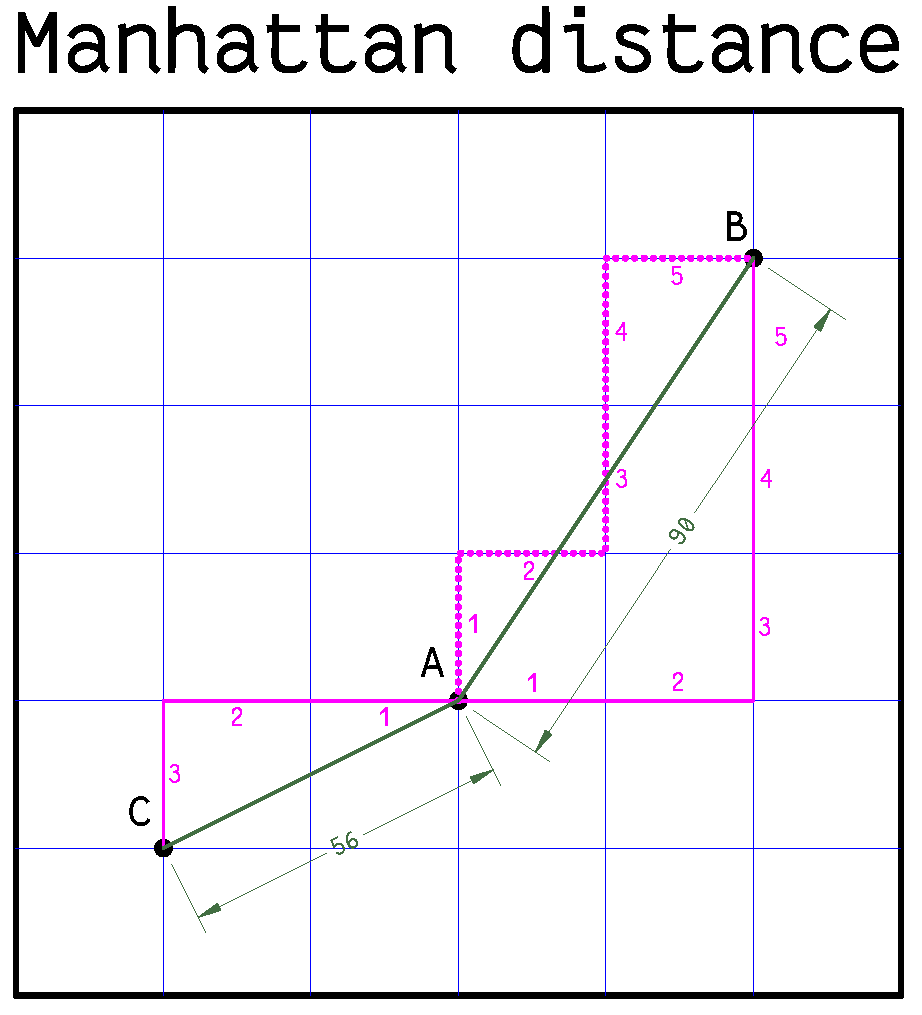
\includegraphics[width=0.75\textwidth]{Graphics/Manhattan}
\end{figure}

In the absolute sum (taxicab or Manhattan-) norm \(\ell_1 = ||\AbsVec{x}||_1 = \sum_{i=1}^n{|\AbsVec{x}_i|} \) the distance between two points is the sum of the absolute differences of their Cartesian coordinates. The name alludes to the grid layout of most streets on the island of Manhattan. A taxicab driving between two intersections drives the distance corresponding to the length of the \skalar{\ell_1}-norm (see fig. \ref{fig:Manh}).

\begin{lstlisting}[caption=Absolute sum norm]
  FUNCTION VectorAbsoluteSumNorm(CONST Vec: VectorTyp): float;

  VAR
    i: WORD;
    Sum: float;

  BEGIN
    IF (VectorLength(Vec) = 0)
      THEN
        BEGIN
          Result := 0;
          EXIT;
        END;
    Sum := 0;
    FOR i := 1 TO VectorLength(Vec) DO
      Sum := Sum + Abs(GetVectorElement(Vec, i));
    Result := Sum;
  END;
\end{lstlisting}

\subsubsection{Vector normalisation}

These are special cases of \skalar{p}-norms, \(||\AbsVec{x}||_p = \sqrt[p]{\sum_{i=1}^n{|\AbsVec{x}_i|^p}} \) for \(p = 1, 2, \infty \), respectively. Vectors can be normalised by dividing all elements by a norm:

\begin{lstlisting}[caption=Normalisation of vector]
  PROCEDURE NormaliseVector(VAR Vec: VectorTyp; Norm: float);

  BEGIN
    DivConstant(Vec, Norm);
  END;
\end{lstlisting}


\subsubsection{Inner (dot) product of a vector}\label{text:dotprod}

The inner product of two vectors \AbsVec{a,b} is a real number \(\AbsVec{a} \odot \AbsVec{b} = \sum_{i=1}^n{(\AbsVec{a}_i \AbsVec{b}_i)} \), the signed area of the parallelogram formed by the vectors. The sign depends on the angle between the vectors (clock- or counter-clockwise).  We use \Name{Neumaier}-addition to prevent the accumulation of error:

\begin{lstlisting}[caption=Inner product of vectors]
  FUNCTION VectorInnerProduct(CONST A, B: VectorTyp): float;

  VAR
    i, n1, n2: WORD;
    x: VectorTyp;

  BEGIN
    n1 := VectorLength(A);
    n2 := VectorLength(B);
    IF (n1 <> n2)
      THEN
        BEGIN
          CH := WriteErrorMessage('Vector error: Inner Product of vectors of unequal length');
          VectorError := true;
          EXIT;
        END;
    IF (n1 = 0)
      THEN
        BEGIN
          Result := 0;
          EXIT;
        END;
    CreateVector(x, n1, 0.0);
    FOR i := 1 TO n1 DO
      SetVectorElement(x, i, GetVectorElement(A, i) * GetVectorElement(B, i));
    Result := NeumaierSum(x);
    DestroyVector(x);
  END;
\end{lstlisting}

\subsubsection{Angle between two vectors}

The angle between two vectors is then calculated by \(\alpha = \frac{\AbsVec{ab}}{|\AbsVec{a}| |\AbsVec{b}|} \):

\begin{lstlisting}[caption=Angle between vectors]
  FUNCTION VectorAngle(CONST A, B: VectorTyp): float;

  VAR
    n1, n2: WORD;

  BEGIN
    n1 := VectorLength(A);
    n2 := VectorLength(B);
    IF (n1 <> n2)
      THEN
        BEGIN
          CH := WriteErrorMessage('Vector-Error: Angle between vectors of unequal dimension');
          VectorError := TRUE;
          EXIT;
        END;
    IF (n1 = 0)
      THEN Result := 0
      ELSE Result := ArcCos(VectorInnerProduct(A, B) /
        (VectorEuklidianNorm(A) * VectorEuklidianNorm(B)));
  END;
\end{lstlisting}

\texttt{TotalSum} and \texttt{TotalProduct} calculate the sum or product over all elements of the vector. Any \acs{NaN} is handled by ignoring that value. Therefore, to calculate the arithmetic or harmonic mean, one cannot simply use \texttt{VectorLength()} to determine the number of actual elements:

\begin{lstlisting}[caption=Number of non-NaN elements]
  FUNCTION ActualElements(CONST A: VectorTyp): WORD;

  VAR
    i, j: WORD;

  BEGIN
    j := 0;
    FOR i := 1 TO VectorLength(A) DO
      IF IsNaN(GetVectorElement(A, i))
        THEN
        ELSE INC(j);
    Result := j;
  END;
\end{lstlisting}


\subsection{Scaling, centering and normalisation of vectors}

To scale a vector to the range \([0\ldots 1] \) we can use
\begin{equation}
  \AbsVec{y} = \frac{\AbsVec{x} - \min{(\AbsVec{x})}}{\max{(\AbsVec{x})} - \min{(\AbsVec{x})}}
\end{equation}
If the data contain outliers, it can be useful to use, say, the 5th and 95th percentile instead of the minimum and maximum. For this reason, we give \texttt{min} and \texttt{max} as parameters of the function rather than determining it within:

\begin{lstlisting}[caption=Scaling a vector]
  PROCEDURE Scale(VAR Vec: VectorTyp; min, max: float);

  VAR
    i: WORD;
    Range: float;

  BEGIN
    Range := max - min;
    FOR i := 1 TO VectorLength(Vec) DO
      SetVectorElement(Vec, i, (GetVectorElement(Vec, i) - min) / Range);
  END;
\end{lstlisting}

A data vector is centered by subtracting the arithmetic mean, so that the new mean becomes zero:
\begin{equation}
  \AbsVec{y} = \AbsVec{x} - \bar{\AbsVec{x}}
\end{equation}


\begin{lstlisting}[caption=Centering a vector]
  PROCEDURE Centre(VAR Vec: VectorTyp);

  VAR
    Mean: float;
    i: WORD;

  BEGIN
    Mean := NeumaierSum(Vec) / ActualElements(Vec);
    FOR i := 1 TO VectorLength(Vec) DO
      SetVectorElement(Vec, i, GetVectorElement(Vec, i) - Mean);
  END;
\end{lstlisting}

\subsection{Vector distance}

The distance between two row vectors (observations) \Vector{a}, \Vector{b} is the sum of the squared differences \( \sum_{i=1}^n(\AbsVec{a}_i - \AbsVec{b}_i)^2 \):

\begin{lstlisting}[caption=]
  FUNCTION SquaredEuklidianDistance(CONST A, B: VectorTyp;
    IgnoreFirst: BOOLEAN): float;

  VAR
    p, i, start: WORD;
    c: CHAR;
    ai, bi, Sum: float;

  BEGIN
    p := VectorLength(A);
    IF VectorLength(B) <> p
      THEN
        BEGIN
          VectorError := TRUE;
          c := WriteErrorMessage('Euklidian distance of two vectors: vectors have unequal length');
          EXIT;
        END;
    Sum := 0;
    IF IgnoreFirst
      THEN Start := 2   // first column study number
      ELSE Start := 1;  // first column data
    FOR i := Start TO p DO
      BEGIN
        ai := GetVectorElement(A, i);
        bi := GetVectorElement(B, i);
        IF IsNaN(ai) OR IsNaN(Bi)
          THEN
            BEGIN
              VectorError := TRUE;
              c := WriteErrorMessage(
                'Euklidian distance of two vectors: vectors contain NaN');
              EXIT;
            END;
        Sum := Sum + Sqr(ai - bi);
      END;
    Result := Sum;
  END;
\end{lstlisting}



\section{Sorting a vector}\label{text:sort}

There are several different sorting algorithms, with different efficiencies with respect to memory requirement and computation speed. For medium numbers of elements (several hundred to a few thousand), the \Name{Shell} sort is often the best compromise, even if values are partially sorted already. This routine, modified from \parencite{Mor-13}, can handle \acs{NaN} elements and sorts them as highest values:
\begin{lstlisting}[caption=Shell sort]
  PROCEDURE ShellSort(VAR t: VectorTyp);

  LABEL
    10;

  VAR
    i, j, k, l, m, nn, NaNs, n, LdN: INTEGER;
    tmp, s: float;

  BEGIN
    NaNs := 0;
    s := -1e300;
    n := VectorLength(t);
    FOR i := 1 TO n DO
      BEGIN
        IF IsNaN(GetVectorElement(t, i))    // check FOR NaN data
          THEN INC(NaNs)
          ELSE IF (GetVectorElement(t, i)) > s
                 THEN s := GetVectorElement(t, i); // AND find largest element OF data vector
      END;
    s := 10 * s;
    IF (NaNs > 0)
      THEN
        FOR i := 1 TO n DO
          IF IsNaN(GetVectorElement(t, i))
            THEN SetVectorElement(t, i, s);
    // replace all NaN WITH very large number so they Move TO END OF vector
    LdN := Trunc(Ln(n) / Const_ln2);
    m := n;
    FOR nn := 1 TO LdN DO
      BEGIN
        m := m DIV 2;
        k := n - m;
        FOR j := 1 TO k DO
          BEGIN
            i := j;
  10:       l := i + m;
            IF (GetVectorElement(t, l) < GetVectorElement(t, i))
              THEN
                BEGIN
                  tmp := GetVectorElement(t, i);
                  SetVectorElement(t, i, GetVectorElement(t, l));
                  SetVectorElement(t, l, tmp);
                  i := i - m;
                  IF i >= 1 THEN GOTO 10;
                END;
          END;
      END;
    IF (NaNs > 0) THEN
      FOR i := Succ(n - NaNs) TO n DO  // change the top NaNs elements back TO NaN
        SetVectorElement(t, i, NaN);
  END;


  END.
\end{lstlisting}

\printbibliography[heading=subbibliography]
\end{refsection}


  % -*- TeX:UK -*-
\chapter{Matrix calculations}
\begin{refsection}


\abstract{Matrices are vectors that have vectors as members. They are used to assign a vector of measured values (columns) to a vector of test subjects (rows). Thus, matrices are used as data structures in multivariate statistics.}

The routines in this unit are based on \parencite{Pre-89,Atk-83,Bor-86,Eng-87,Sed-83,Ste-73,Ren-02}. For the implementation of two-dimensional arrays we use the same method as for vectors. We could use an \texttt{array[1..MaxN, 1..MaxP]}, however, it is more memory efficient to use a ``flat'', one-dimensional array. The conversion of a two-dimensional position \skalar{i, j} into a one-dimensional is done in \texttt{SetVectorElement} and \texttt{GetVectorElement}.

\begin{lstlisting}[caption=]
  type MatrixStruc = record
                       Columns, Rows: word;
                       Data: array[1..MaxVector] of float;
                     end
      MatrixTyp    = ^MatrixStruc;
\end{lstlisting}

The method of error handling is the same too, except that we use the typed constant \texttt{MatrixError} as error flag. Therefore, the interface is

\begin{lstlisting}[caption=Interface of unit Matrix]
  unit Matrix;

  INTERFACE

  USES Math, MathFunc, Vector;

  CONST
    MatrixError: BOOLEAN = FALSE;   { toggle for error condition }

  TYPE
    MatrixStruc = RECORD
      Columns, Rows: WORD;
      Data: ARRAY[1..MaxVector] OF float;
    END;
    MatrixTyp = ^MatrixStruc;

  FUNCTION WriteErrorMessage(TEXT: STRING): CHAR;

  PROCEDURE CreateMatrix(VAR Mat: MatrixTyp; Rows, Columns: WORD; Value: float);

  PROCEDURE DestroyMatrix(VAR Mat: MatrixTyp);

  PROCEDURE ReadMatrix(MedStr: STRING; VAR A: MatrixTyp);

  PROCEDURE WriteMatrix(MedStr: STRING; CONST A: MatrixTyp; ValidFigures: BYTE);

  FUNCTION GetMatrixElement(CONST A: MatrixTyp; Row, Column: WORD): float;

  PROCEDURE SetMatrixElement(VAR A: MatrixTyp; Row, Column: WORD; Value: float);

  PROCEDURE CreateIdentityMatrix(VAR A: MatrixTyp; n: WORD);

  PROCEDURE CreateNullMatrix(VAR A: MatrixTyp; n: WORD);

  PROCEDURE CreateHilbertMatrix(VAR H: MatrixTyp; n: WORD);

  FUNCTION MatrixRows(CONST A: MatrixTyp): WORD;

  FUNCTION MatrixColumns(CONST A: MatrixTyp): WORD;

  { ************************************************************************* }

  PROCEDURE GetRow(CONST A: MatrixTyp; Z: WORD; VAR Vek: VectorTyp);

  PROCEDURE GetColumn(CONST A: MatrixTyp; S: WORD; VAR Vek: VectorTyp);

  PROCEDURE ExchangeColumns(VAR A: MatrixTyp; Column1, Column2: WORD);

  PROCEDURE ExchangeRows(VAR A: MatrixTyp; Row1, Row2: WORD);

  PROCEDURE SetRow(VAR A: MatrixTyp; CONST Vek: VectorTyp; Z: WORD);

  PROCEDURE SetColumn(VAR A: MatrixTyp; CONST Vek: VectorTyp; S: WORD);

  PROCEDURE CopyMatrix(CONST Source: MatrixTyp; VAR Dest: MatrixTyp);

  { *************************** Matrixalgebra ******************************* }

  PROCEDURE MatrixAdd(CONST A, B: MatrixTyp; VAR Res: MatrixTyp);

  PROCEDURE SkalarMultiplikation(VAR A: MatrixTyp; x: float);

  PROCEDURE MatrixInnerProduct(CONST A, B: MatrixTyp; VAR C: MatrixTyp);

  PROCEDURE HadamardSchurProduct(CONST A, B: MatrixTyp; VAR C: MatrixTyp);

  PROCEDURE MatrixDivision(CONST A, B: MatrixTyp; VAR C: MatrixTyp);

  PROCEDURE CenterData(VAR A: MatrixTyp);

  PROCEDURE ChangeMatrixNorm(VAR A: MatrixTyp; Norm: float);

  FUNCTION Determinante(CONST A: MatrixTyp): float;

  FUNCTION MatrixTrace(CONST A: MatrixTyp): float;

  FUNCTION FrobeniusNorm(CONST A: MatrixTyp): float;

  FUNCTION FrobeniusSkalarProduct(CONST A, B: MatrixTyp): float;

  PROCEDURE ERoMultAdd(VAR A: MatrixTyp; Faktor: float; Row1, Row2: WORD);

  PROCEDURE InverseMatrix(VAR A: MatrixTyp);

  PROCEDURE MatrixTranspose(CONST A: MatrixTyp; VAR B: MatrixTyp);

  PROCEDURE AntiSym(CONST A: MatrixTyp; VAR Symmetric, Antisymmetric: MatrixTyp);

  PROCEDURE Diag(VAR Matrix: MatrixTyp);

  PROCEDURE LeadingPrincipleMinors(VAR A: MatrixTyp; VAR V: VectorTyp);

  PROCEDURE NegativeMatrix(VAR A: MatrixTyp);

  { ****************************** spezielle Matrizen *********************** }

  FUNCTION MatrixSquare(CONST A: MatrixTyp): BOOLEAN;

  FUNCTION MatrixSymmetric(VAR A: MatrixTyp): BOOLEAN;

  FUNCTION MatrixLeftTrapezoid(VAR A: MatrixTyp): BOOLEAN;

  FUNCTION MatrixRightTrapezoid(VAR A: MatrixTyp): BOOLEAN;

  FUNCTION MatrixDiagonal(VAR A: MatrixTyp): BOOLEAN;

  FUNCTION MatrixUpperTriangular(VAR A: MatrixTyp): BOOLEAN;

  FUNCTION MatrixLowerTriangular(VAR A: MatrixTyp): BOOLEAN;

  FUNCTION MatrixUpperHessenberg(VAR A: MatrixTyp): BOOLEAN;

  FUNCTION MatrixLowerHessenberg(VAR A: MatrixTyp): BOOLEAN;

  FUNCTION MatrixTridiagonal(VAR A: MatrixTyp): BOOLEAN;

  FUNCTION MatrixPositivDefinite(CONST A: MatrixTyp): BOOLEAN;

  FUNCTION NullMatrix(VAR A: MatrixTyp): BOOLEAN;

  { ***************************** Vector/Matrix ***************************** }

  PROCEDURE DyadicVectorProduct(CONST A, B: VectorTyp; VAR C: MatrixTyp);

  PROCEDURE MultMatrixVector(CONST Mat: MatrixTyp; CONST Vek: VectorTyp;
    VAR Result: VectorTyp);

  PROCEDURE CangeVectorToMatrix(CONST Vek: VectorTyp; VAR Mat: MatrixTyp);

  { ************************* sorting ********************************** }

  PROCEDURE ShellSortMatrix(VAR t: MatrixTyp; Column: WORD);
  { sorts the rows of a matrix by column "Column" }


  IMPLEMENTATION

  VAR
    CH: CHAR;
\end{lstlisting}

\section{Generation and destruction of matrices}


\begin{lstlisting}[caption=Create a new matrix]
  PROCEDURE CreateMatrix(VAR Mat: MatrixTyp; Rows, Columns: WORD; Value: float);

  VAR
    i: WORD;
    x: longword;

  BEGIN
    x := Rows * Columns * SizeOf(float) + 2 * SizeOf(WORD) + 4;
    TRY
      GetMem(Mat, x);
    except
      CH := WriteErrorMessage(' Not enough memory to create matrix');
      MatrixError := true;
      EXIT;
    END;
    Mat^.Columns := Columns;
    Mat^.Rows := Rows;
    FOR i := 1 TO (Rows * Columns) DO
      Mat^.Data[i] := Value;
  END;
\end{lstlisting}


\begin{lstlisting}[caption=Remove a matrix and free its memory]
  PROCEDURE DestroyMatrix(VAR Mat: MatrixTyp);

  VAR
    x: longword;

  BEGIN
    x := MatrixRows(Mat) * MatrixColumns(Mat) * SizeOf(float) + 2 * SizeOf(WORD) + 4;
    FreeMem(Mat, x);
  END;
\end{lstlisting}

Matrices can be read from, and written to, files. The file name is in \texttt{MedStr}. Note that \texttt{'CON'} and \texttt{'PRN'} write to the console or the printer, respectively.

\begin{lstlisting}[caption=Read a matrix from file]
  PROCEDURE ReadMatrix(MedStr: STRING; VAR A: MatrixTyp);

  VAR
    i, j, n, p: WORD;
    x: float;
    Medium: TEXT;

  BEGIN
    Assign(Medium, MedStr);
    Reset(Medium);
    IF IOResult <> 0
      THEN
        BEGIN
          CH := WriteErrorMessage(' Reading a matrix: File not found');
          MatrixError := true;
          EXIT;
        END;
    ReadLn(Medium, n);
    ReadLn(Medium, p);
    IF ((n * p > MaxVector))
      THEN
        BEGIN
          CH := WriteErrorMessage(' Reading a matrix: Matrix too big');
          EXIT;
        END;
    CreateMatrix(A, n, p, 0.0);
    FOR i := 1 TO n DO
      BEGIN
        IF EoF(Medium)
          THEN
            BEGIN
              CH := WriteErrorMessage(' Reading a matrix: Unknown file format');
              MatrixError := true;
              EXIT;
            END;
        FOR j := 1 TO p DO
          BEGIN
            IF EoLn(Medium)
              THEN
                BEGIN
                  CH := WriteErrorMessage(' Reading a matrix: Unknown file format');
                  MatrixError := true;
                  EXIT;
                END;
            Read(Medium, x);
            IF IOResult <> 0
              THEN
                BEGIN
                  CH := WriteErrorMessage(' Reading a matrix: Unknown file format');
                  MatrixError := true;
                  EXIT;
                END;
            SetMatrixElement(A, i, j, x);
          END; { for j }
        ReadLn(Medium);
      END;  { for i }
    Close(Medium);
  END;
\end{lstlisting}


\begin{lstlisting}[caption=Write a matrix to a file]
  PROCEDURE WriteMatrix(MedStr: STRING; CONST A: MatrixTyp; ValidFigures: BYTE);

  VAR
    i, j: WORD;
    Medium: TEXT;

  BEGIN
    Assign(Medium, MedStr);
    Rewrite(Medium);
    Writeln(Medium, A^.Rows);
    Writeln(Medium, A^.Columns);
    IF NOT (IOResult = 0)
      THEN
        BEGIN
          CH := WriteErrorMessage(' Writing a matrix: Illegal File operation');
          MatrixError := true;
          EXIT;
        END;
    FOR i := 1 TO MatrixRows(A) DO
      BEGIN
        FOR j := 1 TO MatrixColumns(A) DO
          Write(Medium, FloatStr(GetMatrixElement(A, i, j), ValidFigures), ' ');
        Writeln(Medium);
      END;
    Close(Medium);
  END;
\end{lstlisting}

\section{Accesing and changing data in a matrix}

\begin{lstlisting}[caption=]
  FUNCTION MatrixRows(CONST A: MatrixTyp): WORD;

  BEGIN
    MatrixRows := A^.Rows;
  END;


  FUNCTION MatrixColumns(CONST A: MatrixTyp): WORD;

  BEGIN
    MatrixColumns := A^.Columns;
  END;


  FUNCTION GetMatrixElement(CONST A: MatrixTyp; Row, Column: WORD): float;

  VAR
    n, p: WORD;

  BEGIN
    n := MatrixRows(A);
    p := MatrixColumns(A);
    IF (Row <= n) AND (Column <= p)
      THEN
        GetMatrixElement := A^.Data[Pred(Row) * p + Column]
      ELSE
        BEGIN
          MatrixError := true;
          CH := WriteErrorMessage(' Attempt to read a non-existent matrix element');
        END;
  END;


  PROCEDURE SetMatrixElement(VAR A: MatrixTyp; Row, Column: WORD; Value: float);

  VAR
    n, p: WORD;

  BEGIN
    n := MatrixRows(A);
    p := MatrixColumns(A);
    IF (Row <= n) AND (Column <= p)
      THEN
        A^.Data[Pred(Row) * p + Column] := Value
      ELSE
        BEGIN
          MatrixError := true;
          CH := WriteErrorMessage(' Attempt to write to a non-existent matrix element');
        END;
  END;
\end{lstlisting}

Just as with vectors, we cannot simply use \arr{A} = \arr{B} to copy a matrix. Copying should be done with the following routine.

\begin{lstlisting}[caption=copy a matrix]
  PROCEDURE CopyMatrix(CONST Source: MatrixTyp; VAR Dest: MatrixTyp);

  VAR
    i, j, p, n: WORD;

  BEGIN
    n := MatrixRows(Source);
    p := MatrixColumns(Source);
    CreateMatrix(Dest, n, p, 0.0);
    IF MatrixError THEN EXIT;
    FOR i := 1 TO n DO
      FOR j := 1 TO p DO
        SetMatrixElement(Dest, i, j, GetMatrixElement(Source, i, j));
  END;
\end{lstlisting}


\begin{lstlisting}[caption=Row operations]
  PROCEDURE GetRow(CONST A: MatrixTyp; Z: WORD; VAR Vek: VectorTyp);

  VAR
    j, m, n: WORD;

  BEGIN
    m := MatrixRows(A);
    n := MatrixColumns(A);
    IF Z > m
      THEN
        BEGIN
          CH := WriteErrorMessage(' Matrix-Error: accessing a non-existent row');
          MatrixError := TRUE;
          EXIT;
        END;
    CreateVector(Vek, n, 0.0);
    FOR j := 1 TO n DO
      SetVectorElement(Vek, j, GetMatrixElement(A, z, j));
  END;

  PROCEDURE SetRow(VAR A: MatrixTyp; CONST Vek: VectorTyp; Z: WORD);

  VAR
    j, n, p: WORD;

  BEGIN
    n := MatrixRows(A);
    p := MatrixColumns(A);
    IF (Z > n) OR (p <> VectorLength(Vek))
      THEN
        BEGIN
          CH := WriteErrorMessage('Matrix-error: set row with illegal parameter');
          MatrixError := TRUE;
          EXIT;
        END;
    FOR j := 1 TO p DO
      SetMatrixElement(A, z, j, GetVectorElement(Vek, j));
  END;


  PROCEDURE ExchangeRows(VAR A: MatrixTyp; Row1, Row2: WORD);

  VAR
    Dummy: float;
    j, n, p: WORD;

  BEGIN
    n := MatrixRows(A);
    p := MatrixColumns(A);
    IF ((Row1 > n) OR (Row2 > n))
      THEN
        BEGIN
          CH := WriteErrorMessage('Matrix-error: accessing non-existant row');
          MatrixError := TRUE;
          EXIT;
        END;
    FOR j := 1 TO p DO
      BEGIN
        Dummy := GetMatrixElement(A, Row1, j);
        SetMatrixElement(A, Row1, j, GetMatrixElement(A, Row2, j));
        SetMatrixElement(A, Row2, j, Dummy);
      END;
  END; { procedure ExchangeRows }
\end{lstlisting}


\begin{lstlisting}[caption=Column operations]
  PROCEDURE GetColumn(CONST A: MatrixTyp; S: WORD; VAR Vek: VectorTyp);

  VAR
    i, n, p: WORD;

  BEGIN
    n := MatrixRows(A);
    p := MatrixColumns(A);
    IF (S > p)
      THEN
        BEGIN
          CH := WriteErrorMessage(' Matrix-error: accessing non-existant column');
          MatrixError := TRUE;
          EXIT;
        END;
    CreateVector(Vek, n, 0.0);
    FOR i := 1 TO n DO
      SetVectorElement(Vek, i, GetMatrixElement(A, i, S));
  END;


  PROCEDURE SetColumn(VAR A: MatrixTyp; CONST Vek: VectorTyp; S: WORD);

  VAR
    i, n, p: WORD;

  BEGIN
    n := MatrixRows(A);
    p := MatrixColumns(A);
    IF (S > p) OR (n <> VectorLength(Vek))
      THEN
        BEGIN
          CH := WriteErrorMessage(' Matrix-error: setting non-existant column');
          MatrixError := TRUE;
          EXIT;
        END;
    FOR i := 1 TO n DO
      SetMatrixElement(A, i, S, GetVectorElement(Vek, i));
  END;


  PROCEDURE ExchangeColumns(VAR A: MatrixTyp; Column1, Column2: WORD);
  { Columns n und m vertauschen }

  VAR
    i, n, p: WORD;
    Dummy: float;

  BEGIN
    n := MatrixRows(A);
    p := MatrixColumns(A);
    IF ((Column1 > p) OR (Column2 > p))
      THEN
        BEGIN
          CH := WriteErrorMessage(' Matrix-errorr: accessing non-existant column');
          MatrixError := TRUE;
          EXIT;
        END;
    FOR i := 1 TO n DO
      BEGIN
        Dummy := GetMatrixElement(A, i, Column1);
        SetMatrixElement(A, i, Column1, GetMatrixElement(A, i, Column2));
        SetMatrixElement(A, i, Column2, Dummy);
      END;
  END;
\end{lstlisting}

The following routine inverts the sign of all elements of a matrix:

\begin{lstlisting}[caption=invert sign of all matrix elements]
  PROCEDURE NegativeMatrix(VAR A: MatrixTyp);

  VAR
    i, j: WORD;

  BEGIN
    FOR i := 1 TO MatrixRows(A) DO
      FOR j := 1 TO MatrixColumns(A) DO
        SetMatrixElement(A, i, j, -GetMatrixElement(A, i, j));
  END;
\end{lstlisting}


\section{Special matrix types}

Some matrices have special properties that simplify calculations with them or allow a particular method to be used.

\subsection{Identity matrix}

In an identity matrix all diagonal elements are unity, all off-diagonal elements zero. It is the neutral element of matrix multiplication.

\begin{lstlisting}[caption=identity matrix]
  PROCEDURE CreateIdentityMatrix(VAR A: MatrixTyp; n: WORD);
  { n*n identity matrix }

  VAR
    i: WORD;

  BEGIN
    CreateMatrix(A, n, n, 0.0);
    IF MatrixError THEN EXIT;
    FOR i := 1 TO n DO
      SetMatrixElement(A, i, i, 1.0);
  END;
\end{lstlisting}

\subsection{The null-matrix}

A matrix \arr{A} is called null-matrix if all its elements are the neutral element of addition, zero. 

\begin{lstlisting}[caption=null matrix]
  PROCEDURE CreateNullMatrix(VAR A: MatrixTyp; n: WORD);

  BEGIN
    CreateMatrix(A, n, n, 0.0);
  END;
\end{lstlisting}

The following function tests, if a matrix is a null-matrix. Again, we set all elements to zero precisely, that are absolute smaller than the constant \texttt{Zero}.

\begin{lstlisting}[caption=are all matrix matrix elements zero?]
  FUNCTION NullMatrix(VAR A: MatrixTyp): BOOLEAN;

  VAR
    i, j: WORD;

  BEGIN
    Result := TRUE;
    FOR i := 1 TO MatrixRows(A) DO
      FOR j := 1 TO MatrixColumns(A) DO
        IF Abs(GetMatrixElement(A, i, j)) > Zero
          THEN
            BEGIN
              Result := FALSE;
              EXIT;
            END
          ELSE
            SetMatrixElement(A, i, j, 0.0);
  END;
\end{lstlisting}

\subsection{The \Name{Hilbert}-matrix}

The \Name{Hilbert}-matrix \(\arr{H}_{n\times n} \) with \(\AbsVec{h}_{ij} = \frac{1}{i+j-1} \) is often used as a test system for matrix inversion and solving linear equations, as it is quite ill-conditioned.

\begin{lstlisting}[caption=Hilbert matrix]
  PROCEDURE CreateHilbertMatrix(VAR H: MatrixTyp; n: WORD);

  VAR
    i, j: WORD;

  BEGIN
    CreateMatrix(H, n, n, 0.0);
    FOR i := 1 TO n DO
      FOR j := 1 TO n DO
        SetMatrixElement(H, i, j, 1 / Pred(i + j));
  END;
\end{lstlisting}

\subsection{The quadratic matrix}


A matrix is quadratic if it has the same number of lines and columns:

\begin{lstlisting}[caption=is matrix square?]
  FUNCTION MatrixSquare(CONST A: MatrixTyp): BOOLEAN;

  BEGIN
    Result := MatrixRows(A) = MatrixColumns(A);
  END;
\end{lstlisting}

\subsection{The symmetric matrix}

A Matrix is symmetric if it is quadratic and \(\AbsVec{x}_{ij} = \AbsVec{x}_{ji} \enspace\forall\enspace i,j \in 1\ldots n \). Since we cannot test for identity of real numbers, we test for the difference being smaller than the typed constant \texttt{Zero}. In that case, we set the upper diagonal to the lower, to avoid numeric difficulties in later calculations.

\begin{lstlisting}[caption=]
  FUNCTION MatrixSymmetric(VAR A: MatrixTyp): BOOLEAN;

  VAR
    i, j, Dimen: WORD;
    x, y: float;

  BEGIN
    Dimen := MatrixRows(A);
    IF NOT (MatrixSquare(A))
      THEN
        BEGIN
          MatrixSymmetric := FALSE;
          EXIT;
        END;
    FOR i := 1 TO Dimen DO
      FOR j := 1 TO Dimen DO
        BEGIN
          x := GetMatrixElement(A, i, j);
          y := GetMatrixElement(A, j, i);
          IF Abs(x - y) > Zero
            THEN
              BEGIN
                MatrixSymmetric := FALSE;
                EXIT;
              END
            ELSE   // make sure they are identical
              SetMatrixElement(A, i, j, GetMatrixElement(A, j, i));
        END;
    MatrixSymmetric := TRUE;
  END;
\end{lstlisting}

\subsection{Trapezoid matrices}

A matrix is left trapezoid, if all elements below the diagonal are zero. A matrix is right trapezoid if all elements above the diagonal are zero. Again, if these elements are smaller than \texttt{Zero}, we set them to 0.0:


 \begin{lstlisting}[caption=is matrix left trapezoid]
  FUNCTION MatrixLeftTrapezoid(VAR A: MatrixTyp): BOOLEAN;

  VAR
    i, j: WORD;

  BEGIN
    Result := FALSE;
    FOR i := 1 TO MatrixRows(A) DO
      FOR j := 1 TO Pred(i) DO
        IF Abs(GetMatrixElement(A, i, j)) > Zero
          THEN EXIT
          ELSE SetMatrixElement(A, i, j, 0.0);
    Result := TRUE;
  END;


  FUNCTION MatrixRightTrapezoid(VAR A: MatrixTyp): BOOLEAN;

  VAR
    i, j: WORD;

  BEGIN
    Result := FALSE;
    FOR i := 1 TO MatrixRows(A) DO
      FOR j := Succ(i) TO MatrixColumns(A) DO
        IF Abs(GetMatrixElement(A, i, j)) > Zero
          THEN EXIT
          ELSE SetMatrixElement(A, i, j, 0.0); // make sure
    Result := TRUE;
  END;
\end{lstlisting}

\subsection{The diagonal matrix and function diag}

If only the diagonal elements are different from zero, we call a matrix diagonal:

\begin{lstlisting}[caption=is matrix  diagonal]
  FUNCTION MatrixDiagonal(VAR A: MatrixTyp): BOOLEAN;

  BEGIN
    Result := MatrixRightTrapezoid(A) AND MatrixLeftTrapezoid(A);
  END;
\end{lstlisting}

The procedure \texttt{Diag} sets all of-diagonal elements of a matrix to zero:

\begin{lstlisting}[caption=set all of-diagonal elements to zero]
  PROCEDURE Diag(VAR Matrix: MatrixTyp);

  VAR
    n, p, i, j: WORD;

  BEGIN
    n := MatrixRows(Matrix);
    p := MatrixColumns(Matrix);
    IF (p <> n)
      THEN
        BEGIN
          CH := WriteErrorMessage('Matrix-error: Diag of a non-square matrix');
          MatrixError := TRUE;
          EXIT;
        END;
    FOR i := 1 TO n DO
      FOR j := Succ(i) TO p DO
        BEGIN
          SetMatrixElement(Matrix, i, j, 0.0);
          SetMatrixElement(Matrix, j, i, 0.0);
        END;
  END;
\end{lstlisting}

\subsection{Triangular matrices}

Square matrices which are trapezoid are called triangular:

\begin{lstlisting}[caption=is matrix triangular?]
  FUNCTION MatrixUpperTriangular(VAR A: MatrixTyp): BOOLEAN;

  BEGIN
    Result := MatrixLeftTrapezoid(A) AND MatrixSquare(A);
  END;


  FUNCTION MatrixLowerTriangular(VAR A: MatrixTyp): BOOLEAN;

  BEGIN
    Result := MatrixRightTrapezoid(A) AND MatrixSquare(A);
  END;
\end{lstlisting}

\subsection{\Name{Hessenberg} matrices}

The elements \(\AbsVec{a}_{ij}, j = i+1 \) are called superdiagonal. A matrix has the upper \Name{Hessenberg} form if it is quadratic and all elements above the superdiagonal are zero. The elements \(\AbsVec{a}_{ij}, j = i-1 \) are called infradiagonal. A matrix has the lower \Name{Hessenberg} form if it is quadratic and all elements below the infradiagonal are zero. If a matrix has both upper and lower \Name{Hessenberg} form, it is called tridiagonal.


\begin{lstlisting}[caption=has matrix the upper Hessenberg form?]
  FUNCTION MatrixUpperHessenberg(VAR A: MatrixTyp): BOOLEAN;

  VAR
    i, j: WORD;

  BEGIN
    Result := FALSE;
    IF NOT (MatrixSquare(A)) THEN EXIT;
    FOR i := 1 TO MatrixRows(A) DO
      FOR j := 1 TO i - 2 DO
        IF Abs(GetMatrixElement(A, i, j)) > Null
          THEN EXIT
          ELSE SetMatrixElement(A, i, j, 0.0);
    Result := TRUE;
  END;


  FUNCTION MatrixLowerHessenberg(VAR A: MatrixTyp): BOOLEAN;

  VAR
    i, j: WORD;

  BEGIN
    Result := FALSE;
    IF NOT (MatrixSquare(A)) THEN EXIT;
    FOR i := 1 TO MatrixRows(A) DO
      FOR j := i + 2 TO MatrixColumns(A) DO
        IF Abs(GetMatrixElement(A, i, j)) > Null
          THEN EXIT
          ELSE SetMatrixElement(A, i, j, 0.0);
    Result := TRUE;
  END;


  FUNCTION MatrixTridiagonal(VAR A: MatrixTyp): BOOLEAN;

  BEGIN
    Result := MatrixUpperHessenberg(A) AND MatrixLowerHessenberg(A);
  END;
\end{lstlisting}

\subsection{Positive and negative definite matrices}

A square matrix is positive definite, if all diagonal elements are \(> 0 \), the largest element is on the diagonal and \(\AbsVec{a}_{ij}^2 < \AbsVec{a}_{ii} * \AbsVec{a}_{jj} \). For such matrices, the \Name{Gauss}-algorithm without pivot search can be used. Their eigenvalues are all \(> 0 \); positive semi-definite matrix have one or more eigenvalues that are \(= 0 \), their rank is equal to the number of eigenvalues \(> 0 \).

\begin{lstlisting}[caption=is matrix positive definite?]
  FUNCTION MatrixPositivDefinite(CONST A: MatrixTyp): BOOLEAN;

  VAR
    i, j: WORD;
    Akt, Max: float;

  BEGIN
    Result := FALSE;
    Max := 0.0;
    IF NOT (MatrixSquare(A)) THEN EXIT;
    FOR i := 1 TO MatrixRows(A) DO
      BEGIN
        Akt := GetMatrixElement(A, i, i);
        IF Akt <= 0 THEN EXIT;
        IF Akt > Max THEN Max := Akt;
      END;
    FOR i := 1 TO MatrixRows(A) DO
      BEGIN
        FOR j := 1 TO Pred(i) DO
          BEGIN
            Akt := GetMatrixElement(A, i, j);
            IF Akt > Max
              THEN EXIT;
            IF Sqr(Akt) >= GetMatrixElement(A, i, i) * GetMatrixElement(A, j, j)
              THEN EXIT;
          END;
        FOR j := Succ(i) TO MatrixColumns(A) DO
        BEGIN
          Akt := GetMatrixElement(A, i, j);
          IF Akt > Max
            THEN EXIT;
          IF Sqr(Akt) >= GetMatrixElement(A, i, i) * GetMatrixElement(A, j, j)
            THEN EXIT;
        END;
      END;
    Result := TRUE;
  END;
\end{lstlisting}


\section{Calculation with matrices}

\subsection{Matrix norms}

The trace of a quadratic matrix is the sum of its diagonal elements:

\begin{equation}
  \mathrm{tr}(\arr{A}_{n \times n}) = \sum_{i=1}^n{\AbsVec{a}_{ii}}
\end{equation}

The following rules apply:
\begin{eqnarray}
  \trace(\arr{A}+\arr{B}) &=& \trace(\arr{A}) + \trace(\arr{B}) \\
  \trace(\arr{AB}) &=& \trace(\arr{BA}) \\
  \trace(\arr{A}^T\arr{A}) &=& \trace(\arr{A}\arr{A}^T) = \sum_{i=1}^{n}{\sum_{j=1}^{p}{a_{ij}^2}}
\end{eqnarray}

\begin{lstlisting}[caption=Trace of a matrix]
  FUNCTION MatrixTrace(CONST A: MatrixTyp): float;

  VAR
    i, n, p: WORD;
    Sum: float;

  BEGIN
    n := MatrixRows(A);
    p := MatrixColumns(A);
    IF (n <> p)
      THEN
        BEGIN
          CH := WriteErrorMessage(' Matrix-error: trace of a matrix that is not square');
          MatrixError := TRUE;
          EXIT;
        END;
    Sum := 0;
    FOR i := 1 TO n DO
      Sum := Sum + GetMatrixElement(A, i, i);
    MatrixTrace := Sum;
  END;
\end{lstlisting}

Matrix-norms \textbf{induced by vector-norms} for a (not necessarily quadratic) matrix \(\arr{A}_{n \times p} \) are:
\begin{align}
   \|A\|_\infty &= \max_{1\leq i\leq n}\sum_{i=1}^p{|a_{ij}|} \\
   \|A\|_1 &= \max_{1\leq j\leq p}\sum_{i=1}^p{|a_{ij}|} \\
   \|A\|_F &= \sqrt{\sum_{i=1}^n{\sum_{j=1}^p{|\AbsVec{a}_{ij}|^2}}}
\end{align}
the maximum absolute row sum, maximum absolute column sum and \Name{Frobenius}-norm, respectively. For example

\begin{tabular}{|ccc|c}
  -3 &  5 &  7 & 15 \\
   2 &  6 &  4 & 12 \\
   0 &  2 &  8 & 10 \\
   \midrule
   5 & 13 & 19 &    \\
\end{tabular}

\( \|A\|_1 = \max(5, 13, 19) = 19 \) and \(\|A\|_\infty = \max(15, 12, 10) = 15 \). The trace \(\mathrm{tr}(\arr{A}) = -3 + 6 + 8 = 11 \). The \Name{Frobenius}-Norm is
\begin{equation}
  \|A\|_F = \sqrt{(-3^2+5^2+7^2) + (2^2+6^2+4^2) + (0^2+2^2+8^2)} = \sqrt{207} = 14.4
\end{equation}

\textbf{Entry-wise norms} treat a matrix \(\arr{A}_{n\times p} \) as vector of length \(np \). Then
\begin{equation}
  \|A\|_q = \sqrt[q]{\sum_{i=1}^{n\times p}{|\AbsVec{a}_{i}|^q}}
\end{equation}
with the special cases \(q=2 \) the \Name{Frobenius}-norm and \(q=\infty \) the maximum norm.

The \textbf{Schatten-norms} are defined as follows:
\begin{equation}
  \|\arr{A}\|_q = \sqrt[q]{\sum_{i=1}^{\min(n,p)}{\sigma_i^q}}
\end{equation}
with \(\sigma_i \) the i-th singular value (\Foreign{vide infra}) of \arr{A}.

\begin{lstlisting}[caption=]
  FUNCTION FrobeniusNorm(CONST A: MatrixTyp): float;

  VAR
    i, j, n, p: WORD;
    Sum: extended;

  BEGIN
    n := MatrixRows(A);
    p := MatrixColumns(A);
    Sum := 0.0;
    FOR i := 1 TO n DO
      FOR j := 1 TO p DO
        Sum := Sum + Sqr(GetMatrixElement(A, i, j));
    FrobeniusNorm := Sqrt(Sum);
  END;
\end{lstlisting}

The \Name{Frobenius} scalar product of two matrices \(\|\arr{A,B}\| = \mathrm{trace}(\arr{A}^T \arr{B}) \). It follows that \(\|\arr{A}\|_F = \sqrt{\|\arr{A}^T, \arr{A}\|} \):

\begin{lstlisting}[caption=Frobenius skalar product]
  FUNCTION FrobeniusSkalarProduct(CONST A, B: MatrixTyp): float;

  VAR
    CH: CHAR;
    C, D: MatrixTyp;
    n, p: WORD;

  BEGIN
    n := MatrixRows(A);
    p := MatrixColumns(A);
    IF NOT ((n = MatrixRows(B)) AND (p = MatrixColumns(B)))
      THEN
        BEGIN
          CH := WriteErrorMessage(
            ' Matrix-error: Frobenius-Skalar product of incompatible matrices');
          MatrixError := TRUE;
          EXIT;
        END;
    MatrixTranspose(A, C);          // C = A^T
    MatrixInnerProduct(C, B, D);    // D = A^T B
    FrobeniusSkalarProduct := MatrixTrace(D);
    DestroyMatrix(C);
    DestroyMatrix(D);
  END;
\end{lstlisting}

\subsection{Determinant}

To calculate the determinant, we will need a little helper function, that adds a multiple of row 1 to row 2. It is also required for the solution of systems of equations.

\begin{lstlisting}[caption=add multiple of row 1 to row 2]
  PROCEDURE ERoMultAdd(VAR A: MatrixTyp; Faktor: float; Row1, Row2: WORD);

  VAR
    j: WORD;

  BEGIN
    FOR j := 1 TO MatrixColumns(A) DO
      SetMatrixElement(A, Row2, j, GetmatrixElement(A, Row2, j) +
        GetMatrixElement(A, Row1, j) * Faktor);
  END;
\end{lstlisting}


The determinant of a square matrix \(|\arr{A}_{n \times n}| \) is defined as the sum of all \skalar{n}! possible products of \skalar{n} elements such that
\begin{enumerate}
  \item{each product contains one element from every row and every column}
  \item{the factors in each product are written so that the column subscripts appear in order of magnitude and each product is then preceded by a plus or minus sign according to whether the number of inversions in the row subscripts is even or odd.}
  \item{An inversion occurs whenever a larger number precedes a smaller one.}
\end{enumerate}
For a \(3\times 3 \) matrix, this is
\begin{gather}
   |\arr{A}| = \det\begin{pmatrix}
                      a_{11} & a_{12} & a_{13} \\
                      a_{21} & a_{22} & a_{23} \\
                      a_{31} & a_{32} & a_{33}
                   \end{pmatrix} \\
                   =   a_{11} a_{22} a_{33} + a_{12} a_{23} a_{31} + a_{13} a_{32} a_{21} - a_{31} a_{22} a_{13} - a_{32} a_{23} a_{11} - a_{33} a_{12} a_{21}
\end{gather}
For larger matrices, this becomes unwieldy.

The following special cases exist:
\begin{itemize}
  \item{For diagonal matrices, the determinant is the product of the diagonal elements \(|\arr{X}| = \prod_{i=1}^{n}(\AbsVec{x}_i) \). }
  \item{If a square matrix is singular, then its determinant is \( |\arr{X}| = 0 \), if it is non-singular, the determinant \( |\arr{X}| \neq\ 0 \).}
  \item{If a matrix is \textbf{positive definite}, then its determinant is positive.}
  \item{\( |\arr{X}^T| = |\arr{X}| \), \(|\arr{X}^{-1}| = |\arr{X}|^{-1} \)}
\end{itemize}

\begin{lstlisting}[caption=Determinant of a matrix]
  FUNCTION Determinante(CONST A: MatrixTyp): float;

  VAR
    PartialDeter, Multiplier: float;
    Row, ReferenceRow: WORD;
    DetEqualsMaxError: BOOLEAN;
    Copy: MatrixTyp;

    PROCEDURE Pivot(ReferenceRow: WORD; VAR PartialDeter: float;
    VAR DetEqualsMaxError: BOOLEAN);
       {- This procedure searches the ReferenceRow column of the matrix Data for
          the first non-MaxError element below the diagonal. If it finds one, then
          the procedure switches rows so that the non-MaxError element is on the
          diagonal. Switching rows changes the determinant by a factor of -1;
          this change is returned in PartialDeter. If it doesn't find one, the
          matrix is singular and the Determinant is MaxError (DetEqualsMaxError = true
          is returned.  -}

    VAR
      NewRow: INTEGER;

    BEGIN
      DetEqualsMaxError := TRUE;
      NewRow := ReferenceRow;
      WHILE DetEqualsMaxError AND (NewRow < MatrixRows(Copy)) DO
        BEGIN  { Try to find a row with a non-MaxError    }
          NewRow := Succ(NewRow);
          IF Abs(GetMatrixElement(Copy, NewRow, ReferenceRow)) > MaxError
            THEN
              BEGIN
                ExchangeRows(Copy, NewRow, ReferenceRow); { Switch these two rows }
                DetEqualsMaxError := FALSE;
                PartialDeter := -PartialDeter;  { Switching rows changes }
              END; { the determinant by a factor of -1 }
        END;
    END; { procedure Pivot }

  BEGIN  { Determinante }
    IF MatrixRows(A) = 1
      THEN
        BEGIN
          Result := GetMatrixElement(A, 1, 1);
          EXIT;
        END;
    CopyMatrix(A, Copy);
    IF MatrixError THEN EXIT;
    DetEqualsMaxError := FALSE;
    PartialDeter := 1;
    ReferenceRow := 0;
    { Make the matrix upper triangular }
    WHILE NOT (DetEqualsMaxError) AND (ReferenceRow < Pred(MatrixRows(Copy))) DO
      BEGIN
        INC(ReferenceRow);
        { If diagonal element is MaxError then switch rows }
        IF Abs(GetMatrixElement(Copy, ReferenceRow, ReferenceRow)) < MaxError
          THEN Pivot(ReferenceRow, PartialDeter, DetEqualsMaxError);
        IF NOT (DetEqualsMaxError)
          THEN
            FOR Row := Succ(ReferenceRow) TO MatrixRows(Copy) DO
            { Make the ReferenceRow element of this row MaxError }
              IF Abs(GetMatrixElement(Copy, Row, ReferenceRow)) > MaxError
                THEN
                  BEGIN
                    Multiplier :=
                      -GetMatrixElement(Copy, Row, ReferenceRow) /
                      GetMatrixElement(Copy, ReferenceRow, ReferenceRow);
                    EROmultAdd(Copy, Multiplier, ReferenceRow, Row);
                  END;
        { Multiply the diagonal Term into PartialDeter }
        PartialDeter := PartialDeter * GetMatrixElement(Copy, ReferenceRow, ReferenceRow);
      END; { while }
    IF DetEqualsMaxError
      THEN
        Result := 0
      ELSE
        Result := PartialDeter * GetMatrixElement(Copy, MatrixRows(Copy),
        MatrixColumns(Copy));
    DestroyMatrix(Copy);
  END; { function Determinante }
\end{lstlisting}

Example:
\begin{gather}
   \det
   \begin{pmatrix}
      1.00 & 2.00 & 0.00 & -1.00 \\
     -1.00 & 4.00 & 3.00 & -0.50 \\
      2.00 & 2.00 & 1.00 & -3.00 \\
      0.00 & 0.00 & 3.00 & -4.00
   \end{pmatrix} = 21.0
\end{gather}

\subsubsection{Leading principle minors}

The leading principle minors of a symmetric matrix \(\arr{A}_{n \times n} \) are the determinants of the sub-matrices with \(1, 2\ldots n \) rows and columns, starting with the upper left corner. \arr{A} is positive definite if all principal minors are positive, it is negative definite if all even principle minors are positive, all odd negative (\Name{Sylvester}-criterion).

\begin{lstlisting}[caption=Leading principle minors]
  PROCEDURE LeadingPrincipleMinors(VAR A: MatrixTyp; VAR V: VectorTyp);
  // Implementierung nicht elegant, bei großen Matrizen Wiederholung vermeiden

  VAR
    n, i, j, k: WORD;
    B: MatrixTyp;

  BEGIN
    IF NOT MatrixSymmetric(A)
      THEN
        BEGIN
          CH := WriteErrorMessage( 'Matrix-error: leading principle minors of a non-square matrix');
          MatrixError := TRUE;
          EXIT;
        END;
    n := MatrixRows(A);
    CreateVector(V, n, 0.0);
    FOR i := 1 TO n DO
      BEGIN
        CreateMatrix(B, i, i, 0.0);
        FOR j := 1 TO i DO
          FOR k := 1 TO i DO
            SetMatrixElement(B, j, k, GetMatrixElement(A, j, k));
        SetVectorElement(V, i, Determinante(B));
        DestroyMatrix(B);
      END;
    FOR i := 1 TO n DO
      IF Abs(GetVectorElement(V, i)) < Zero THEN SetVectorElement(V, i, 0);
  END;
\end{lstlisting}

The following routine changes the norm of a matrix:

\begin{lstlisting}
  PROCEDURE ChangeMatrixNorm(VAR A: MatrixTyp; Norm: float);

  VAR
    SP: float;
    i, j: WORD;

  BEGIN
    IF Abs(Norm) < MaxError
      THEN
        BEGIN
          CH := WriteErrorMessage(' Norm of a matrix must be greater than 0');
          MatrixError := true;
          EXIT;
        END;
    SP := 0;
    FOR i := 1 TO MatrixRows(A) DO
      FOR j := 1 TO MatrixColumns(A) DO
        SP := SP + Sqr(GetMatrixElement(A, i, j));
    IF Abs(SP) < MaxError
      THEN
        BEGIN
          CH := WriteErrorMessage(' Norm of a matrix: no solution');
          MatrixError := true;
          EXIT;
        END;
    Norm := Norm / Sqrt(SP);
    FOR i := 1 TO MatrixRows(A) DO
      FOR j := 1 TO MatrixColumns(A) DO
        SetMatrixElement(A, i, j, GetMatrixElement(A, i, j) * norm);
  END;
\end{lstlisting}

\subsection{Matrix transpose}

The transpose of a matrix \(\arr{A}^T \) is generated by turning the matrix by \ang{90}, so that rows turn into columns and \Foreign{vice versa}. In the following routine, the input matrix and its transpose must be different:

\begin{lstlisting}[caption=]
  PROCEDURE MatrixTranspose(CONST A: MatrixTyp; VAR B: MatrixTyp);

  VAR
    i, j, n, p: WORD;

  BEGIN
    n := MatrixRows(A);
    p := MatrixColumns(A);
    CreateMatrix(B, p, n, 0.0);
    FOR i := 1 TO n DO
      FOR j := 1 TO p DO
        SetMatrixElement(B, j, i, GetMatrixElement(A, i, j));
  END;
\end{lstlisting}

For matrices with complex elements, the \textbf{conjugate (\Name{Hermite}ian) transpose} \( \arr{A}^* \) is obtained from the transpose by calculating the complex conjugate of each element. For real matrices, \( \arr{A}^* = \arr{A}^T \). Matrices, for which \( \arr{A}^* \arr{A} = \arr{A} \arr{A}^* \) are called \textbf{normal}.

\subsubsection{Orthogonal vectors and matrices}

Two vectors are said to be orthogonal (perpendicular) if they have the same size and \(\AbsVec{a}^T\AbsVec{b} = 0 \). If \(\sqrt{\AbsVec{a}^T \AbsVec{a}} \) is the length of a vector, then \(\AbsVec{c} = \frac{\AbsVec{a}}{\sqrt{\AbsVec{a}^T \AbsVec{a}}} \) is said to be normalised and \(\AbsVec{c}^T \AbsVec{c} = 1 \).

A matrix \(\arr{C} \) is orthogonal if all its columns \(\AbsVec{c}_1, \AbsVec{c}_2, \ldots, \AbsVec{c}_p \) are normalised and orthogonal to each other. Then \(\arr{C}^T\arr{C} = \arr{C}\arr{C}^T = \mathbf{I} \), thus the rows are also normalised and orthogonal.

If \(\AbsVec{z} = \arr{C}\AbsVec{x} \) and \(\arr{C} \) is orthogonal, then
\begin{equation}
  \AbsVec{z}^T\AbsVec{z} = (\arr{C}\AbsVec{x})^T (\arr{C}\AbsVec{x}) =
    \AbsVec{x}^T\arr{C}^T\arr{C}\AbsVec{x} = \AbsVec{x}^T\mathbf{I}\AbsVec{x} = \AbsVec{x}^T\AbsVec{x}
\end{equation}
and \(\AbsVec{x} \) and \(\AbsVec{z} \) have the same length, but the axes are rotated.

\subsection{Matrix inverse}
The inverse of a matrix \(\arr{A}^{-1} \) is defined as \(\arr{A} \arr{A}^{-1} = \arr{I} \) the identity matrix (diagonal matrix with all diagonal elements equal 1.0), it is equivalent to the reciprocal of a number:

\begin{lstlisting}[caption=Inverse of a matrix]
  PROCEDURE InverseMatrix(VAR A: MatrixTyp);

  VAR
    i, j, m, n, p: WORD;
    NoExch: 0..MaxVector;
    Exch: ARRAY [1..MaxVector, 1..2] OF INTEGER;


    PROCEDURE Transform(m: WORD);

    VAR
      B: MatrixTyp;
      i, j: WORD;
      Pivot: float;

    BEGIN
      CopyMatrix(A, B);
      Pivot := GetMatrixElement(B, m, m);
      IF Abs(Pivot) <= MaxError THEN
      BEGIN
        CH := WriteErrorMessage('Matrix error: inversion of singular matrix');
        MatrixError := true;
        EXIT;
      END;
      FOR i := 1 TO n DO
        FOR j := 1 TO n DO
          IF i <> m
            THEN
              IF j <> m
                THEN
                  SetMatrixElement(B, i, j, GetMatrixElement(A, i, j) -
                     GetMatrixElement(A, i, m) * GetMatrixElement(A, m, j) / Pivot)
                ELSE
                  SetMatrixElement(B, i, j, GetMatrixElement(A, i, j) / Pivot)
            ELSE IF j <> m
                   THEN SetMatrixElement(B, i, j, -GetMatrixElement(A, i, j) / Pivot)
                   ELSE SetMatrixElement(B, i, j, 1 / Pivot);
      DestroyMatrix(A);
      CopyMatrix(B, A);
      DestroyMatrix(B);
    END; { Transform }

  BEGIN { InverseMatrix }
    NoExch := 0;
    m := MatrixRows(A);
    n := MatrixColumns(A);
    IF m <> n
      THEN
        BEGIN
          CH := WriteErrorMessage(' Matrix error: inversion of non-quadratic matrix');
          MatrixError := true;
          EXIT;
        END;
    FOR i := 1 TO m DO
      BEGIN
        p := i;
        FOR j := Succ(i) TO n DO
          IF Abs(GetMatrixElement(A, j, i)) > Abs(p)
            THEN p := j;
        IF p <> i
          THEN
            BEGIN
              INC(NoExch);
              Exch[NoExch, 1] := i;
              Exch[NoExch, 2] := p;
              ExchangeRows(A, i, p);
            END;
        Transform(i);
        IF MatrixError THEN EXIT;
      END;
    FOR i := NoExch DOWNTO 1 DO
      ExchangeColumns(A, Exch[i, 2], Exch[i, 1]);
  END; { InverseMatrix }
\end{lstlisting}

Example:
\begin{gather}
   \begin{pmatrix}
      1.00 & 2.00 & 0.00 & -1.00 \\
     -1.00 & 4.00 & 3.00 & -0.50 \\
      2.00 & 2.00 & 1.00 & -3.00 \\
      0.00 & 0.00 & 3.00 & -4.00
   \end{pmatrix}^{-1} =
   \begin{pmatrix}
     -1.95 & 0.19 &  1.57 & -0.71 \\
      0.76 & 0.05 & -0.36 &  0.07 \\
     -1.90 & 0.38 &  1.14 & -0.43 \\
     -1.43 & 0.29 &  0.86 & -0.57
   \end{pmatrix}
\end{gather}

\subsection{Matrix sums and differences}

Matrices, if they have the same size, are added by adding their elements \(\AbsVec{c}_{ij} = \AbsVec{a}_{ij} + \AbsVec{b}_{ij} \):

\begin{lstlisting}[caption=Sum of two matrices]
  PROCEDURE MatrixAdd(CONST A, B: MatrixTyp; VAR Res: MatrixTyp);
  { Elementweise Addition zweier Matrizen. }

  VAR
    i, j, Rows, Columns: WORD;

  BEGIN
    Rows := MatrixRows(A);
    Columns := MatrixColumns(A);
    IF ((Rows <> MatrixRows(B)) OR (Columns <> MatrixColumns(B)))
      THEN
        BEGIN
          CH := WriteErrorMessage(
            ' Matrix error: addition of matrices not of the same size');
          MatrixError := true;
          EXIT;
        END;
    CreateMatrix(Res, Rows, Columns, 0);
    FOR i := 1 TO Rows DO
      FOR j := 1 TO Columns DO
        SetMatrixElement(Res, i, j, GetMatrixElement(A, i, j) + GetMatrixElement(B, i, j));
  END;
\end{lstlisting}

A matrix is multiplied with a scalar by multiplying all elements with the scalar:

\begin{lstlisting}[caption=]
  PROCEDURE SkalarMultiplikation(VAR A: MatrixTyp; x: float);
  { Elementweise Multiplikation einer Matrix mit einem Skalar }

  VAR
    i, j: WORD;

  BEGIN
    FOR i := 1 TO MatrixRows(A) DO
      FOR j := 1 TO MatrixColumns(A) DO
        SetMatrixElement(A, i, j, GetMatrixElement(A, i, j) * x);
  END;
\end{lstlisting}

\subsection{Matrix inner and \Name{Hadamard-Schur} product}

The inner product of a matrix is defined by the inner products of all rows of the first matrix with all columns of the second. Hence the number of columns of the first and the number of rows of the second matrix need to be identical (\skalar{k}): \(\arr{A}_{n\times p} \arr{B}_{p\times q} = \arr{C}_{n\times q}, \AbsVec{c}_{ij} = \AbsVec{a}_{i\cdot} \AbsVec{b}_{\cdot j} = \AbsVec{a}_{i1}\AbsVec{b}_{1j} + \AbsVec{a}_{i2}\AbsVec{b}_{2j}\ldots \AbsVec{a}_{ip}\AbsVec{b}_{pj} = \sum_{k}{\AbsVec{a}_{ik} \AbsVec{b}_{kj}} \). Calculation via the vector dot product has the advantage that the summation is performed by \Name{Neumaier}-process, preventing error accumulation. Note that for square matrices of equal size both \(\arr{AB} \) and \(\arr{BA} \) are defined, but \(\arr{AB} \neq \arr{BA} \).


\begin{lstlisting}[caption=inner product of two matrices]
  PROCEDURE MatrixInnerProduct(CONST A, B: MatrixTyp; VAR C: MatrixTyp);

  VAR
    i, j: WORD;
    Col, Row: VectorTyp;

  BEGIN
    IF MatrixColumns(A) <> MatrixRows(B)
      THEN
        BEGIN
          CH := WriteErrorMessage(' Matrix error: multiplication of A.Columns <> B.Rows');
          MatrixError := true;
          EXIT;
        END;
    CreateMatrix(C, MatrixRows(A), MatrixColumns(B), 0.0);
    FOR i := 1 TO MatrixRows(A) DO
      FOR j := 1 TO MatrixColumns(B) DO
      BEGIN
        GetRow(A, i, Row);
        GetColumn(B, j, Col);
        SetMatrixElement(C, i, j, VectorInnerProduct(Row, Col));
        DestroyVector(Row);
        DestroyVector(Col);
      END;
  END;
\end{lstlisting}

Much rarer used than the inner product of two matrices is the \Name{Hadamard-Schur}- (element-wise) product:

\begin{lstlisting}[caption=Hadamard-Schur product of two matrices]
  PROCEDURE HadamardSchurProduct(CONST A, B: MatrixTyp; VAR C: MatrixTyp);

  VAR
    i, j, n, p: WORD;

  BEGIN
    n := MatrixRows(A);
    IF (n <> MatrixRows(B))
      THEN
        BEGIN
          CH := WriteErrorMessage(' Hadamard-Schur multiplication: A.Rows <> B.Rows');
          MatrixError := true;
          EXIT;
        END;
    p := MatrixColumns(A);
    IF (p <> MatrixColumns(B))
      THEN
        BEGIN
          CH := WriteErrorMessage( 'Hadamard-Schur multiplication: A.Columns <> B.Columns');
          MatrixError := true;
          EXIT;
        END;
    CreateMatrix(C, n, p, 0.0);
    FOR i := 1 TO n DO
      FOR j := 1 TO p DO
        SetMatrixElement(C, i, j, GetMatrixElement(A, i, j) * GetMatrixElement(B, i, j));
  END;
\end{lstlisting}

\subsection{Matrix division}

\begin{lstlisting}[caption=division of two matrices]
  PROCEDURE MatrixDivision(CONST A, B: MatrixTyp; VAR C: MatrixTyp);

  VAR
    Rows, Columns, i, j, k: WORD;
    M, N: MatrixTyp;

  BEGIN
    Rows := MatrixRows(A);
    Columns := MatrixColumns(A);
    IF (Rows <> Columns) OR (Columns <> MatrixRows(B))
      THEN
        BEGIN
          CH := WriteErrorMessage(
            ' Matrix division: A.Columns <> B.Rows or A not quadratic');
          MatrixError := TRUE;
          EXIT;
        END;
    CopyMatrix(A, M);
    CopyMatrix(B, N);
    IF MatrixError THEN EXIT;
    FOR j := 1 TO Rows DO
      BEGIN
        IF GetMatrixElement(M, j, j) = 0
          THEN
            FOR k := j TO Rows DO
              IF GetMatrixElement(M, k, j) <> 0
                THEN
                  BEGIN
                    ExchangeRows(M, j, k);
                    ExchangeRows(N, j, k);
                  END
                ELSE IF k = Rows
                       THEN
                         BEGIN
                           CH := WriteErrorMessage(' Matrix division: no solution');
                           MatrixError := TRUE;
                           EXIT;
                         END;
        FOR i := Succ(j) TO Rows DO
          SetMatrixElement(M, i, j, GetMatrixElement(M, i, j) / GetMatrixElement(M, j, j));
        FOR i := Succ(j) TO Rows DO
          BEGIN
            FOR k := Succ(j) TO Rows DO
              SetMatrixElement(M, i, k, GetMatrixElement(M, i, k) -
                GetMatrixElement(M, j, k) * GetMatrixElement(M, i, j));
            FOR k := 1 TO MatrixColumns(N) DO
              SetMatrixElement(N, i, k, GetMatrixElement(N, i, k) -
                GetMatrixElement(N, j, k) * GetMatrixElement(M, i, j));
          END;
      END;
    FOR i := Rows DOWNTO 1 DO
      FOR k := 1 TO MatrixColumns(N) DO
        BEGIN
          FOR j := Succ(i) TO Columns DO
            SetMatrixElement(N, i, k, GetMatrixElement(N, i, k) -
              GetMatrixElement(N, j, k) * GetMatrixElement(M, i, j));
          SetMatrixElement(N, i, k, GetMatrixElement(N, i, k) /
            GetMatrixElement(M, i, i));
        END;
    CopyMatrix(N, C);
    DestroyMatrix(M);
    DestroyMatrix(N);
  END;
\end{lstlisting}

\begin{lstlisting}[caption=]
  PROCEDURE CenterData(VAR A: MatrixTyp);

  VAR
    Data: VectorTyp;
    j, Columns: WORD;

  BEGIN
    Columns := MatrixColumns(A);
    FOR j := 1 TO Columns DO
      BEGIN
        GetColumn(A, j, Data);
        Centre(Data);
        SetColumn(A, Data, j);
        DestroyVector(Data);
      END;
  END;
\end{lstlisting}


\subsection{Symmetric and anti-symmetric matrices}

The following routine splits a matrix into a symmetric and an anti-symmetric:

\begin{lstlisting}[caption=split matrix in symmetric and anti-symmetic]
  PROCEDURE AntiSym(CONST A: MatrixTyp; VAR Symmetric, Antisymmetric: MatrixTyp);

  VAR
    Dimen, i, j: WORD;

  BEGIN
    Dimen := MatrixRows(A);
    IF Dimen <> MatrixColumns(A)
      THEN
        BEGIN
          CH := WriteErrorMessage('Antisymmetrical of an unsymmetric Matrix');
          MatrixError := true;
          EXIT;
        END;
    FOR i := 1 TO Dimen DO
      FOR j := 1 TO Dimen DO
        BEGIN
          SetMatrixElement(AntiSymmetric, i, j, 0.5 *
            (GetMatrixElement(A, i, j) + GetMatrixElement(A, j, i)));
          SetMatrixElement(Symmetric, i, j, GetMatrixElement(A, i, j) -
            GetMatrixElement(Antisymmetric, i, j));
        END;
  END;
\end{lstlisting}

\subsection{Matrix exponentiation}

The matrix exponential is defined for square matrices \( \arr{X} \in \mathbb{R}_{n\times n} \) or \( \mathbb{C}_{n\times n} \) by a \Name{Taylor}-series:
\begin{equation}
  \mathrm{e}^\arr{X} = \sum_{k=0}^\infty{\frac{\arr{X}^k}{k!}} = \arr{I} + \arr{X} + \frac{\arr{X}^2}{2} + \ldots
\end{equation}
, which always converges.

The matrix exponential shares a number of properties with the exponential on real numbers:
\begin{itemize}
  \item{\( \mathrm{e}^\mathbf{0} = \arr{I} \) }
  \item{\( \mathrm{e}^{a\arr{X}} \mathrm{e}^{b\arr{X}} = \mathrm{e}^{(a+b)\arr{X}} \forall a, b \in \mathbb{C}\) }
  \item{\( \mathrm{e}^\arr{X} \mathrm{e}^{-\arr{X}} = \mathrm{e}^{(1-1)\arr{X}} = \mathrm{e}^\mathbf{0} = \arr{I} \)}
  \item{\( (\mathrm{e}^\arr{X})^{-1} = \mathrm{e}^{-\arr{X}}\) }
  \item{\( \mathrm{e}^\arr{X+Y} = \mathrm{e}^\arr{X} \mathrm{e}^\arr{Y} \) for commuting matrices (\arr{XY} = \arr{YX}). }
  \item{\( \mathrm{e}^{\arr{X}^T} = (\mathrm{e}^\arr{X})^T \)}
  \item{\( \det(\mathrm{e}^\arr{X}) = \mathrm{e}^{\trace(\arr{X})} \) }
  \item{\( \mathrm{e}^{\diag(x_1, x_2, \ldots x_n)} = \diag(\mathrm{e}^{x_1}, \mathrm{e}^{x_2}, \ldots \mathrm{e}^{x_n}) \)}
  \item{\( \mathrm{e}^\arr{X} \) is always invertible. }
\end{itemize}

One applications of the matrix exponential is solving systems of ordinary differential equations, for example starting value problems:
\begin{equation}
  \frac{d}{dt} y(t) = \arr{X}y(t),\quad y(t_0) = y_0
\end{equation}
for square matrix \arr{X} is given by
\begin{equation}
   y(t) = \mathrm{e}^{(t-t_0) \arr{X}} y_0
\end{equation}

For algorithms for matrix exponentials see \parencite{Mol-03,Li-11, Boc-89}.

\section{Calculations with vectors and matrices}

\subsection{Dyadic vector product}

The dyadic vector product multiplies two vectors, resulting in a matrix:
\begin{equation}
  \arr{C}_{n\times p} = \AbsVec{a}_n \otimes \AbsVec{b}_p\quad \AbsVec{c}_{i,j} = \AbsVec{a}_i \times \AbsVec{b}_j
\end{equation}

\begin{lstlisting}[caption=]
  PROCEDURE DyadicVectorProduct(CONST A, B: VectorTyp; VAR C: MatrixTyp);

  VAR
    Row, Column: WORD;

  BEGIN
    CreateMatrix(C, A^.Length, B^.Length, 0.0);
    FOR Row := 1 TO A^.Length DO
      FOR Column := 1 TO B^.Length DO
        SetMatrixElement(C, Row, Column, GetVectorElement(A, Row) *
          GetVectorElement(B, Column));
  END;
\end{lstlisting}

\subsection{Product of a matrix and a vector}

\begin{equation}
  \AbsVec{C}_n = \arr{A}_{n\times p} \star \AbsVec{b}_p\hspace{10mm} \AbsVec{c}_i = \sum_{j=1}^p{\AbsVec{a}_{ij} \times \AbsVec{b}_j}
\end{equation}

\begin{lstlisting}[caption=multiply matrix and vector]
  PROCEDURE MultMatrixVector(CONST Mat: MatrixTyp; CONST Vek: VectorTyp;
    VAR Result: VectorTyp);

  VAR
    Row, Column: WORD;
    Sum: float;

  BEGIN
    IF NOT (MatrixColumns(Mat) = VectorLength(Vek))
      THEN
        BEGIN
          CH := WriteErrorMessage(' Matrix and vector have different number of rows');
          MatrixError := true;
          EXIT;
        END;
    CreateVector(Result, MatrixRows(Mat), 0.0);
    FOR Row := 1 TO MatrixRows(Mat) DO
      BEGIN
        Sum := 0;
        FOR Column := 1 TO MatrixColumns(Mat) DO
          Sum := Sum + GetMatrixElement(Mat, Row, Column) + GetVectorElement(Vek, Column);
        SetVectorElement(Result, Row, Sum);
      END;
  END;
\end{lstlisting}

\subsection{Change a vector to a matrix with one row}

\begin{lstlisting}[caption=change vector to one-dimensional matrix]
  PROCEDURE CangeVectorToMatrix(CONST Vek: VectorTyp; VAR Mat: MatrixTyp);

  VAR
    j: WORD;

  BEGIN
    CreateMatrix(Mat, VectorLength(Vek), 1, 0.0);
    FOR j := 1 TO VectorLength(Vek) DO
      SetMatrixElement(Mat, j, 1, GetVectorElement(Vek, j));
  END;
\end{lstlisting}

\section{Sort rows of a matrix by value of a column}

It is often necessary to sort all rows of a matrix so that a particular column is sorted. We use basically the same routine as for sorting vectors (see \ref{text:sort} on page \pageref{text:sort}.
\begin{lstlisting}[caption=sort matrix]
  PROCEDURE ShellSortMatrix(VAR t: MatrixTyp; Column: WORD);

  LABEL
    10;

  VAR
    i, j, k, l, m, nn, NaNs, n, LdN: INTEGER;
    s: float;
    tmp1, tmp2: VectorTyp;

  BEGIN
    NaNs := 0;
    s := -MaxRealNumber;
    n := MatrixRows(t);
    FOR i := 1 TO n DO
      BEGIN
        IF IsNaN(GetMatrixElement(t, i, Column))    // check forR NaN data
          THEN INC(NaNs)
          ELSE IF (GetMatrixElement(t, i, Column)) > s
                 THEN
                   s := GetMatrixElement(t, i, Column); // and find largest element of data vector
      END;
    s := 10 * s;
    IF (NaNs > 0)
      THEN
        FOR i := 1 TO n DO
          IF IsNaN(GetMatrixElement(t, i, Column))
            THEN SetMatrixElement(t, i, Column, s);
    // replace all NaN WITH very large number so they Move TO END OF vector
    LdN := Trunc(Ln(n) / Const_ln2);
    m := n;
    FOR nn := 1 TO LdN DO
      BEGIN
        m := m DIV 2;
        k := n - m;
        FOR j := 1 TO k DO
          BEGIN
            i := j;
  10:       l := i + m;
            IF (GetMatrixElement(t, l, Column) < GetMatrixElement(t, i, Column))
              THEN
                BEGIN
                  GetRow(t, i, tmp1);
                  GetRow(t, l, tmp2);
                  SetRow(t, tmp2, i);
                  SetRow(t, tmp1, l);
                  DestroyVector(tmp1);
                  DestroyVector(tmp2);
                  i := i - m;
                  IF i >= 1 THEN GOTO 10;
                END;
          END;
      END;
    IF (NaNs > 0)
      THEN
        FOR i := Succ(n - NaNs) TO n DO  // change the top NaNs elements back TO NaN
          SetMatrixElement(t, i, Column, NaN);
  END;

  END. { unit Matrix }
\end{lstlisting}

     % -*- TeX:UK -*-
\section{Solving systems of linear equations}

The system
\begin{equation}
\left\{
        \begin{array}{c@{\;}c@{\;}l}
           \AbsVec{a}_{11} \AbsVec{x}_{1} + \AbsVec{a}_{12} \AbsVec{x}_{2}  + \ldots + \AbsVec{a}_{1p} \AbsVec{x}_{p} & = & \AbsVec{b}_{1} \\
           \AbsVec{a}_{21} \AbsVec{x}_{1} + \AbsVec{a}_{22} \AbsVec{x}_{2}  + \ldots + \AbsVec{a}_{2p} \AbsVec{x}_{p} & = & \AbsVec{b}_{2} \\
           \ldots                                                                                                     &   & \ldots         \\
           \AbsVec{a}_{n1} \AbsVec{x}_{1} + \AbsVec{a}_{n2} \AbsVec{x}_{2}  + \ldots + \AbsVec{a}_{np} \AbsVec{x}_{p} & = & \AbsVec{b}_{n} \\
        \end{array}
\right.
\end{equation}
with known coefficients \(\arr{A} \), known right hand side \(\AbsVec{b}_{i} \) and unknown solutions \(\AbsVec{x} \) can be written in matrix terminology:
\begin{gather}
  \begin{pmatrix}
     \AbsVec{a}_{11} & \AbsVec{a}_{12} & \ldots & \AbsVec{a}_{1p} \\
     \AbsVec{a}_{21} & \AbsVec{a}_{22} & \ldots & \AbsVec{a}_{2p} \\
          \ldots     &                 &        &                 \\
     \AbsVec{a}_{n1} & \AbsVec{a}_{n2} & \ldots & \AbsVec{a}_{np}
  \end{pmatrix} \times
  \begin{pmatrix}
     \AbsVec{x}_{1}  &  \AbsVec{x}_{2} & \ldots & \AbsVec{x}_{p}
  \end{pmatrix} =
  \begin{pmatrix}
     \AbsVec{b}_{1} \\
     \AbsVec{b}_{2} \\
     \ldots         \\
     \AbsVec{b}_{n}
  \end{pmatrix}, \hspace{10mm}
  \arr{A}_{n\times p} \times \AbsVec{X}_{p} = \AbsVec{B}_{n}
\end{gather}
There should be as many equations as unknown (\( n = p \)), thus \arr{A} is square \parencite{Atk-83, Bor-86, Eng-87, Pre-89, Sed-83, Ste-73, Ren-02}.

\begin{lstlisting}[caption=Interface of SystemSolve]
  UNIT SystemSolve;

  INTERFACE

  USES Math, MathFunc, Vector, Matrix;

  CONST
    SystemError: StrArrayType = ('ok', 'dimension error', 'matrix singular',
      'MaxIter < 1', 'no conversion', 'evaluation short-circuited',
      '', 'matrix not symmetric', 'not enough memory', '', '', '');

  FUNCTION MakeUpperTriangular(VAR Koeff : MatrixTyp; VAR Right : VectorTyp) : BYTE;

  FUNCTION HadamardConditionNumber (VAR Mat : MatrixTyp) : double;

  FUNCTION GaussElimination(CONST Coefficients: MatrixTyp;
      VAR RightSide, Solution: VectorTyp): BYTE;

  FUNCTION PartialPivoting(CONST Coefficients: MatrixTyp;
      VAR RightSide, Solution: VectorTyp): BYTE;

  FUNCTION LU_Decompose(CONST Coefficients: MatrixTyp;
      VAR Decomp, Permute: MatrixTyp): BYTE;

  FUNCTION LU_Solve(CONST Decomp, Permute: MatrixTyp; CONST RightSide: VectorTyp;
      VAR Solution: VectorTyp): BYTE;

  FUNCTION Householder (CONST A : MatrixTyp; VAR Q, R : MatrixTyp) : BYTE;

  IMPLEMENTATION

  VAR CH  : CHAR;
\end{lstlisting}

\subsection{Private routines}

\begin{lstlisting}[caption=]
  FUNCTION MakeUpperTriangular(VAR Koeff : MatrixTyp; VAR Right : VectorTyp) : BYTE;

  VAR Multiplier               : double;
      Row, ReferenceRow, Dimen : WORD;

    FUNCTION Pivot(ReferenceRow: INTEGER) : BYTE;
          { This procedure searches the ReferenceRow column of the Coefficients
            matrix for the first non-MaxError element below the diagonal. If it
            finds one, then the procedure switches rows so that the non-MaxError
            element is on the diagonal. It also switches the corresponding
            elements in the Constants vector. If it doesn't find one, the
            matrix is singular and no solution exists (Error = 2 is returned). }

    VAR NewRow : INTEGER;
        Dummy  : double;

    BEGIN
      Result := 2;          { No solution exists }
      NewRow := ReferenceRow;
      WHILE (Result > 0) AND (NewRow < Dimen) DO
        BEGIN    { Try to find a row with a non-MaxError diagonal element    }
          NewRow := Succ(NewRow);
          IF Abs(GetMatrixElement(Koeff, NewRow, ReferenceRow)) > MaxError
            THEN
              BEGIN
                ExchangeRows(Koeff, NewRow, ReferenceRow);
                Dummy := GetVectorElement(Right, NewRow);
                SetVectorElement(Right, NewRow, GetVectorElement(Right, ReferenceRow));
                SetVectorElement(Right, ReferenceRow, Dummy);
                Result := 0;    { Solution may exist }
              END;
        END;
    END; { procedure Pivot }

  BEGIN { procedure UpperTriangular }
    Dimen := MatrixRows(Koeff);
    ReferenceRow := 0;
    Result := 0;
    WHILE ((Result = 0) AND (ReferenceRow < Pred(Dimen))) DO
      BEGIN
        INC(ReferenceRow);  { Check to see if the main diagonal element is MaxError }
        IF Abs(GetMatrixElement(Koeff, ReferenceRow, ReferenceRow)) < MaxError
          THEN Result := Pivot(ReferenceRow);
        IF Result = 0
          THEN
            FOR Row := Succ(ReferenceRow) TO Dimen DO
          { Make the ReferenceRow element of this row MaxError }
              IF Abs(GetMatrixElement(Koeff, Row, ReferenceRow)) > MaxError
                THEN
                  BEGIN
                    Multiplier := -GetMatrixElement(Koeff, Row, ReferenceRow) / GetMatrixElement(Koeff, ReferenceRow, ReferenceRow);
                    EROmultAdd(Koeff, Multiplier, ReferenceRow, Row);
                    SetVectorElement(Right, Row, GetVectorElement(Right, Row) + Multiplier * GetVectorElement(Right, ReferenceRow));
                  END;
      END; { while }
    IF Abs(GetMatrixElement(Koeff, MatrixRows(Koeff), MatrixColumns(Koeff))) < MaxError
      THEN Result := 2;    { No solution }
  END; { procedure UpperTriangular }
\end{lstlisting}

\begin{lstlisting}[caption=]
  PROCEDURE BackwardSubst (VAR Koeff : MatrixTyp; VAR Right, Solution : VectorTyp);
  { This procedure applies backwards substitution to the upper triangular
    Coefficients matrix and Constants vector. The resulting vector is the
    solution to the set of equations and is stored in the vector Solution. }

  VAR Term, Row, Dimen : WORD;
      Sum              : double;

  BEGIN
    Dimen := MatrixRows(Koeff);
    FOR Term := Dimen DOWNTO 1 DO
      BEGIN
        Sum := 0;
        FOR Row := Succ(Term) TO Dimen DO
          Sum := Sum + GetMatrixElement(Koeff, Term, Row) * GetVectorElement(Solution, Row);
        SetVectorElement(Solution, Term, (GetVectorElement(Right, Term) - Sum) / GetMatrixElement(Koeff, Term, Term));
    END;
  END; { procedure BackwardsSub }
\end{lstlisting}

\begin{lstlisting}[caption=Test if matrix is suitable]
  FUNCTION Initial(CONST Coefficients : MatrixTyp; VAR RightSide, Solution : VectorTyp) : BYTE;

  VAR Dimen : WORD;

  BEGIN
    Result := 0;
    Dimen := MatrixRows(Coefficients);
    IF ((Dimen < 1) OR (Dimen <> MatrixColumns(Coefficients)) OR (Dimen <> VectorLength(RightSide)))
      THEN
        Result := 1
      ELSE
        IF Dimen = 1
          THEN
            IF Abs(GetMatrixElement(Coefficients, 1, 1)) < MaxError
              THEN Result := 2
              ELSE SetVectorElement(Solution, 1, GetVectorElement(RightSide, 1) / GetMatrixElement(Coefficients, 1, 1));
  END; { procedure Initial }
\end{lstlisting}

\subsection{The condition number}

The matrix \arr{A} may  be well conditioned, that is, small changes in the elements \(\AbsVec{b} \) will produce only small changes in the solution \(\AbsVec{x} \). Ill conditioned matrices, on the other hand, produce large changes in the solution for small changes in \AbsVec{b}. If \AbsVec{e} is the error in \AbsVec{b} and \arr{A} is not singular, then the error of \(\arr{A}^{-1}\AbsVec{b} \) will be \(\arr{A}^{-1}\AbsVec{E} \) and the relative error will be
\begin{equation}
  \kappa(\arr{A}) = \frac{\frac{||\arr{A}^{-1}\AbsVec{E}||}{||\arr{A}^{-1}\AbsVec{B}||}}{\frac{||\AbsVec{E}||}{||\AbsVec{B}||}}
  = \left(\frac{||\arr{A}^{-1}\AbsVec{E}||}{||\AbsVec{E}||}\right) \left(\frac{||\AbsVec{B}||}{||\arr{A}^{-1}\AbsVec{B}||} \right) = ||\arr{A}^{-1}|| \times ||\arr{A}||
\end{equation}
\( \kappa \) is called the \textbf{condition number} of \arr{A}. Most commonly, the \Name{Frobenius}-norm is used for its calculation. Note that the condition number is a property of the matrix \arr{A}, not the algorithm used for its solution or the numerical precision of the computer.

\begin{lstlisting}[caption=Condition Number]
  FUNCTION HadamardConditionNumber (VAR Mat : MatrixTyp) : double;

  VAR n, i, j           : WORD;
      res               : BYTE;
      Decomp, Permute   : MatrixTyp;
      temp, cond        : double;

  BEGIN
    n := MatrixRows(Mat);
    IF NOT(MatrixSymmetric(Mat))
      THEN
        BEGIN
          CH := WriteErrorMessage(' Hadamard condition number of a non-symmetric matrix');
          Result := NaN;
          EXIT;
        END;
    res := LU_Decompose(Mat, Decomp, Permute);
    IF MatrixError
      THEN
        BEGIN
          Result := NaN;
          EXIT;
        END;
    IF res = 2
      THEN
        Result := 0    // singular matrix
      ELSE
        BEGIN
          cond := 1.0;
          FOR i := 1 TO n DO
            BEGIN
              temp := 0.0;
              FOR j := 1 TO n DO
                temp := temp + Sqr(GetMatrixElement(Mat, i, j));
              cond := cond * GetMatrixElement(Decomp, i, i) / Sqrt(temp);
            END;
          Result := Abs(cond);
        END;
    DestroyMatrix(Decomp);
    DestroyMatrix(Permute);
  END;
\end{lstlisting}

\subsection{Over- and under-determined systems}

If there are more (independent) equations \skalar{n} than unknowns \skalar{p} (overdetermined system) we have an error-minimisation (linear least squares) problem. If there are fewer equations than unknowns (or some equations are linear combinations), then there will be \(p-n \) solution vectors (underdetermined system). These situations can be handled with singular value decomposition.

The routines for system solving return the following error codes:

\begin{tabular}{ll}
  0 & everything ok \\
  1 & dimension error (number of vars \(\neq \) number of equations) \\
  2 & matrix singular \\
  3 & MaxIter < 0 \\
  4 & MaxIter exceeded \\
  5 & evaluation short-circuited  \\
  6 &  \\
  7 & matrix not symmetric \\
  8 & not enough memory \\
\end{tabular}

\subsection{Example}
\begin{gather}
  \begin{pmatrix}
      1.00 & 2.00 & 0.00 & -1.00 \\
     -1.00 & 4.00 & 3.00 & -0.50 \\
      2.00 & 2.00 & 1.00 & -3.00 \\
      0.00 & 0.00 & 3.00 & -4.00
  \end{pmatrix} \times
  \begin{pmatrix}
     -1.00 & 2.00 & 3.00 -7.00
  \end{pmatrix} =
  \begin{pmatrix}
     10.0 \\
     21.5 \\
     26.0 \\
     37.0
  \end{pmatrix}
\end{gather}


\subsection{\Name{Gauss}ian elimination}

The \Name{Gauss}ian elimination method is used to solve systems of equations. The matrix is converted into the upper triangular form, then the solution is calculated by back-substitution (\( \AbsVec{x}_m, \AbsVec{x}_{m-1}\ldots \AbsVec{x}_1 \)). The system has no solution if one or more diagonal elements of the triangular matrix are zero (singular matrix). The method is fast, but sensitive to rounding errors when elements of the diagonal are small compared to elements below them in the same column.

\begin{lstlisting}[caption=]
  FUNCTION GaussElimination(CONST Coefficients : MatrixTyp;
    VAR RightSide, Solution : VectorTyp) : BYTE;

  VAR Error : BYTE;
      Dimen : WORD;
      Koeff : MatrixTyp;
      Right : VectorTyp;

  BEGIN { procedure Gaussian_Elimination }
    Dimen := MatrixRows(Coefficients);
    Result := Initial(Coefficients, RightSide, Solution);
    IF result <> 0 THEN EXIT;
    CreateVector(Right, Dimen, 0.0);
    CreateVector(Solution, Dimen, 0.0);
    CopyVector(RightSide, Right);
    IF VectorError
      THEN
        BEGIN
          VectorError := FALSE;
          Result := 8;
          EXIT;
        END;
    CopyMatrix(Coefficients, Koeff);
    IF MatrixError
      THEN
        BEGIN
          MatrixError := FALSE;
          Result := 8;
          EXIT;
        END;
    IF MatrixRows(Koeff) > 1
      THEN
        BEGIN
          Error := MakeUpperTriangular(Koeff, Right);
          IF Error = 0 THEN BackwardSubst(Koeff, Right, Solution);
        END;
    Result := Error;
    DestroyVector(Right);
    DestroyMatrix(Koeff);
  END; { procedure Gaussian_Elimination }
\end{lstlisting}

\subsection{\Name{Gauss}-elimination with partial pivoting}

In this method lines of matrix and right side are exchanged to ensure that all diagonal elements are larger than the elements below them. This method is more stable, but slower than the simple \Name{Gauss} elimination.

\begin{lstlisting}[caption=]
  FUNCTION PartialPivoting(CONST Coefficients: MatrixTyp;
    VAR RightSide, Solution: VectorTyp): BYTE;

  VAR Error : BYTE;
      Dimen : WORD;
      Koeff : MatrixTyp;
      Right : VectorTyp;

  BEGIN  { procedure PartialPivoting }
    Dimen := MatrixRows(Coefficients);
    Result := Initial(Coefficients, RightSide, Solution);
    IF result <> 0 THEN EXIT;
    CopyMatrix(Coefficients, Koeff);
    IF MatrixError
      THEN
        BEGIN
          MatrixError := FALSE;
          Result := 8;
          EXIT;
        END;
    CreateVector(Solution, Dimen, 0.0);
    CopyVector(RightSide, Right);
    IF VectorError
      THEN
        BEGIN
          VectorError := FALSE;
          Result := 8;
          EXIT;
        END;
    IF Dimen > 1
      THEN
        BEGIN
          Error := MakeUpperTriangular(Koeff, Right);
          IF Error = 0 THEN BackwardSubst(Koeff, Right, Solution);
        END;
    Result := Error;
    DestroyMatrix(Koeff);
    DestroyVector(Right);
  END; { Partial_Pivoting }
\end{lstlisting}

\subsection{LU-decomposition}

The matrix \arr{A} is decomposed into a upper triangular matrix \arr{U} and a lower triangular matrix \arr{L}. Then
\begin{equation}
  \arr{L} \times \arr{U} = \arr{A}
\end{equation}
and
\begin{equation}
  \arr{A} \times \AbsVec{X} = (\arr{L} \times \arr{U}) \times \AbsVec{X} = \arr{L} \times (\arr{U} \times \AbsVec{X}) = \AbsVec{B}
\end{equation}
Taking advantage of the triangular shape of \arr{L} and \arr{U}, we first solve for \(\arr{L} \AbsVec{Y} = \AbsVec{B} \), then for \(\arr{U} \AbsVec{X} = \AbsVec{Y} \). This algorithm is only \(O(n^2) \), and once the decomposition has been performed, it can be used to solve for several right hand sides, if desired.

\begin{lstlisting}[caption=LU-decomposition]
  FUNCTION LU_Decompose(CONST Coefficients : MatrixTyp; VAR Decomp, Permute : MatrixTyp): BYTE;

  VAR Error: BYTE;
      Koeff, Upper, Lower: MatrixTyp;
      Dimen: WORD;


    FUNCTION RowColumnMult(VAR Lower, Upper: MatrixTyp; Row, Column: WORD): double;
      { Function return: dot product of row Row of Lower and column Column of Upper }

    VAR Term : INTEGER;
        Sum  : double;

    BEGIN
      Sum := 0;
      FOR Term := 1 TO Pred(Row) DO
        Sum := Sum + GetMatrixElement(Lower, Row, Term) * GetMatrixElement(Upper, Term, Column);
      Result := Sum;
    END; { RowColumnMult }


    PROCEDURE Pivot(ReferenceRow: WORD; VAR Error: BYTE);
       { This procedure searches the ReferenceRow column of the Coefficients
         matrix for the element in the Row below the main diagonal which
         produces the largest value of Coefficients[Row, ReferenceRow] - Sum
         (for K=1 to pred(ReferenceRow) of Upper[Row, k] - Lower[k, ReferenceRow]
        If it finds one, then the procedure switches rows so that this element
        is on the main diagonal. The procedure also switches the corresponding
        elements in the Permute matrix and the Lower matrix. If the largest
        value of the above expression is MaxError, then the matrix is singular and
        no solution exists (Error = 2 is returned).   }

    VAR PivotRow, Row      : WORD;
        ColumnMax, TestMax : double;

    BEGIN { procedure Pivot }
      { First, find the row with the largest TestMax }
      PivotRow := ReferenceRow;
      ColumnMax := Abs(GetMatrixElement(Koeff, ReferenceRow, ReferenceRow) -
        RowColumnMult(Lower, Upper, ReferenceRow, ReferenceRow));
      FOR Row := Succ(ReferenceRow) TO Dimen DO
        BEGIN
          TestMax := Abs(GetMatrixElement(Koeff, Row, ReferenceRow) - RowColumnMult(Lower, Upper, Row, ReferenceRow));
          IF TestMax > ColumnMax
            THEN
              BEGIN
                PivotRow := Row;
                ColumnMax := TestMax;
              END;
        END;
      IF PivotRow <> ReferenceRow
        THEN   { Second, switch these two rows }
          BEGIN
            ExchangeRows(Koeff, PivotRow, ReferenceRow);
            ExchangeRows(Lower, PivotRow, ReferenceRow);
            ExchangeRows(Permute, PivotRow, ReferenceRow);
          END
        ELSE { If ColumnMax is MaxError, no solution exists }
          IF ColumnMax < MaxError
            THEN Error := 2;
    END; { procedure Pivot }


    PROCEDURE Decompose(VAR Error: BYTE);
       { This procedure decomposes the Coefficients matrix into two triangular
         matrices, a lower and an upper one.  The lower and upper matrices are
         combined into one matrix, Decomp.  The permutation matrix, Permute,
         records the effects of partial pivoting.  }

    VAR Term, Index: INTEGER;

      PROCEDURE Initialize;
            { This procedure initializes Lower and Upper to the MaxError matrix
              and Permute to the identity matrix. }

      BEGIN
        CreateMatrix(Upper, Dimen, Dimen, 0.0);
        CreateMatrix(Lower, Dimen, Dimen, 0.0);
        CreateIdentityMatrix(Permute, Dimen);
        IF MatrixError
          THEN
            BEGIN
              MatrixError := FALSE;
              Error := 8;
            END;
      END; { procedure Initialize }

    BEGIN { Decompose }
      Initialize;
      { partial pivoting on row 1 }
      Pivot(1, Error);
      IF Error = 0
        THEN
          BEGIN
            SetMatrixElement(Lower, 1, 1, 1);
            SetMatrixElement(Upper, 1, 1, GetMatrixElement(Koeff, 1, 1));
            FOR Term := 1 TO Dimen DO
              BEGIN
                SetMatrixElement(Lower, Term, 1, GetMatrixElement(Koeff, Term, 1) / GetMatrixElement(Upper, 1, 1));
                SetMatrixElement(Upper, 1, Term, GetMatrixElement(Koeff, 1, Term) / GetMatrixElement(Lower, 1, 1));
              END;
          END;
      Term := 1;
      WHILE (Error = 0) AND (Term < Pred(Dimen)) DO
        BEGIN
          Term := Succ(Term); { perform partial pivoting on row Term }
          Pivot(Term, Error);
          SetMatrixElement(Lower, Term, Term, 1);
          SetMatrixElement(Upper, Term, Term,
             GetMatrixElement(Koeff, Term, Term) - RowColumnMult(Lower, Upper, term, term));
          IF Abs(GetMatrixElement(Upper, Term, Term)) < MaxError
            THEN
              Error := 2   { no solutions }
            ELSE
              FOR Index := Succ(Term) TO Dimen DO
                BEGIN
                  SetMatrixElement(Upper, Term, Index, GetMatrixElement(Koeff, Term, Index) - RowColumnMult(Lower, Upper, Term, Index));
                  SetMatrixElement(Lower, Index, Term, (GetMatrixElement(Koeff, Index, Term) - RowColumnMult(Lower, Upper, Index, Term)) /
                      GetMatrixElement(Upper, Term, Term));
                END;
        END;
      SetMatrixElement(Lower, Dimen, Dimen, 1);
      SetMatrixElement(Upper, Dimen, Dimen, GetMatrixElement(Koeff, Dimen, Dimen) - RowColumnMult(Lower, Upper, Dimen, Dimen));
      IF Abs(GetMatrixElement(Upper, Dimen, Dimen)) < MaxError THEN Error := 2;
      { Combine the upper and lower triangular matrices into one }
      CopyMatrix(Upper, Decomp);
      FOR Term := 2 TO Dimen DO
        FOR Index := 1 TO Pred(Term) DO
          SetMatrixElement(Decomp, Term, Index, GetMatrixElement(Lower, Term, Index));
      DestroyMatrix(Upper);
      DestroyMatrix(Lower);
    END; { procedure Decompose }

  BEGIN { LU_Decompose }
    Dimen := MatrixRows(Coefficients);
    CopyMatrix(Coefficients, Koeff);
    IF MatrixError
      THEN
        BEGIN
          MatrixError := FALSE;
          Result := 8;
          EXIT;
        END;
    IF Dimen < 1
      THEN
        Error := 1
      ELSE
        BEGIN
          Error := 0;
          IF Dimen = 1
            THEN
              BEGIN
                CopyMatrix(Koeff, Decomp);
                SetMatrixElement(Permute, 1, 1, 1);
              END
            ELSE
              Decompose(Error);
        END;
    Result := Error;
    DestroyMatrix(Koeff);
  END; { LU_Decompose }
\end{lstlisting}

\begin{lstlisting}[caption=Solve system]
  FUNCTION LU_Solve(CONST Decomp, Permute : MatrixTyp; CONST RightSide : VectorTyp;
                    VAR Solution : VectorTyp): BYTE;

  VAR Error    : BYTE;
      Dimen    : WORD;
      DEC, Per : MatrixTyp;
      Right    : VectorTyp;


    PROCEDURE FindSolution;
       { The Decom matrix contains a lower and upper triangular matrix. This
         procedure performs a two step backwards substitution to compute the
         solution to the system of equations.  First, forward substitution is
         applied to the lower triangular matrix and Constants vector yielding
         PartialSolution.  Then backwards substitution is applied to the Upper
         matrix and the PartialSolution vector yielding Solution.  }

    VAR PartialSolution : Vectortyp;
        Term, Index     : WORD;
        Sum             : double;

    BEGIN { FindSolution }
      { First solve the lower triangular matrix }
      CreateVector(PartialSolution, Dimen, 0.0);
      SetVectorElement(PartialSolution, 1, GetVectorElement(Right, 1));
      FOR Term := 2 TO Dimen DO
        BEGIN
          Sum := 0;
          FOR Index := 1 TO Pred(Term) DO
            IF Term = Index
            THEN
              Sum := Sum + GetVectorElement(PartialSolution, Index)
            ELSE
              Sum := Sum + GetMatrixElement(DEC, Term, Index) * GetVectorElement(PartialSolution, Index);
          SetVectorElement(PartialSolution, Term, GetVectorElement(Right, Term) - Sum);
        END;
      { Then solve the upper triangular matrix }
      SetVectorElement(Solution, Dimen, GetVectorElement(PartialSolution,Dimen) / GetMatrixElement(DEC, Dimen, Dimen));
      FOR Term := Pred(Dimen) DOWNTO 1 DO
        BEGIN
          Sum := 0;
          FOR Index := Succ(Term) TO Dimen DO
            Sum := Sum + GetMatrixElement(DEC, Term, Index) * GetVectorElement(Solution, Index);
          SetVectorElement(Solution, Term, (GetVectorElement(PartialSolution, Term) - Sum) / GetMatrixElement(DEC, Term, Term));
        END;
      DestroyVector(PartialSolution);
    END; { procedure FindSolution }


    PROCEDURE PermuteRightSide;

    VAR Row, Column   : WORD;
        Entry         : double;
        TempConstants : VectorTyp;

    BEGIN
      CreateVector(TempConstants, Dimen, 0.0);
      FOR Row := 1 TO Dimen DO
        BEGIN
          Entry := 0;
          FOR Column := 1 TO Dimen DO
            Entry := Entry + GetMatrixElement(Per, Row, Column) * GetVectorElement(Right, Column);
          SetVectorElement(TempConstants, Row, Entry);
        END;
      CopyVector(TempConstants, Right);
      DestroyVector(TempConstants);
    END; { PermuteRightSide }

  BEGIN { Solve_LU_Decompostion }
    Dimen := MatrixRows(Decomp);
    CopyMatrix(Decomp, DEC);
    CopyMatrix(Permute, Per);
    CreateVector(Solution, Dimen, 0.0);
    IF MatrixError
      THEN
        BEGIN
          MatrixError := FALSE;
          Result := 8;
          EXIT;
        END;
    CopyVector(RightSide, Right);
    IF VectorError
      THEN
        BEGIN
          VectorError := FALSE;
          Result := 8;
          EXIT;
        END;
    IF Dimen < 1
      THEN
        Error := 1
      ELSE
        BEGIN
          Error := 0;
          PermuteRightSide;
          FindSolution;
        END;
    Result := Error;
    DestroyMatrix(DEC);
    DestroyMatrix(Per);
  END; { procedure LU_Solve }
\end{lstlisting}


\subsection{The QR-factorisation}

The QR-factorisation decomposes a \(\arr{A}_{n\times p} \)-matrix (\( n \geq p \)) into the product of an unitary (orthogonal if \arr{A} is square, real and of full rank) matrix \(\arr{Q}_{n\times n} \) (\Foreign{i.e.}, \(\arr{QQ}^T = \arr{Q}^T\arr{Q} = \arr{I} \)) and an upper triangular matrix \(\arr{R}_{n\times p} \):
\begin{equation}
  \arr{A} = \arr{QR}
\end{equation}
The bottom \((n-p) \) rows of \arr{R} consist entirely of zeroes. Then
\begin{equation}
  \arr{A} = \arr{QR} = \arr{Q} \begin{pmatrix}
                                  \hat{\arr{R}} \\
                                  \mathbf{0}
                               \end{pmatrix}
\end{equation}
The upper triangular matrix \(\hat{\arr{R}}_{p\times p} \) is regular with diagonal elements \(\hat{\arr{R}}_{ii} \neq 0 \) if \(\mathrm{rk}(\arr{A}) = p \) (see below).

The factorisation is used to calculate linear least-square and eigenvalue problems. Also, since \(\det(\arr{A}) = \det(\arr{Q}) * \det(\arr{R}) \) and \(\det(\arr{Q}) = \pm 1 \), \(|\det(\arr{A})| = |\det(\arr{R})| = |\prod_{i=1}^p{\skalar{r}_{ii}}| = |\prod_{i=1}^p{\sigma_{ii}}| \) (or \(|\prod_{i=1}^p{\lambda_{ii}}| \) if \arr{A} is square). Thus, QR-factorisation can be used to cheaply calculate the products of singular or eigenvalues of \arr{A}. Because \arr{QR} have better condition numbers than \arr{A}, this factorisation is also used for linear inverse problems.

It is also possible to work with a lower triangular matrix \arr{L}, or to exchange the matrices (RQ-, QL- and LQ-factorisation).

There are three important methods for QR-factorisation:
\begin{description}
  \item[\Name{Gram–Schmidt} process]{easy to implement, but numerically unstable}
  \item[\Name{Householder} reflection]{medium complexity, stable, not parallelisable}
  \item[\Name{Givens} rotation]{complex to implement, stable, parallelisable}
\end{description}
Since we need a stable algorithm, but haven't worried about parallelisation with any of the other routines, we'll use \Name{Householder} reflection.

\subsubsection{\Name{Householder} reflection}

Multiplication of a vector, for example the \skalar{k}-th column vector of \arr{A}, \(\AbsVec{a}_{\cdot,k} \), with a \Name{Householder} matrix
\begin{equation}
  \arr{H} = \arr{I} - \frac{2}{\AbsVec{u}^T \odot \AbsVec{u}}\enspace \AbsVec{u} \otimes \AbsVec{u}^T
\end{equation}
reflects this vector by a plane defined by its normal \AbsVec{u}. Note that \(\AbsVec{u} \otimes \AbsVec{u}^T \) is the outer (dyadic) product, and hence a matrix, while \(\AbsVec{u}^T \odot \AbsVec{u} \) is the inner (dot) product of the vectors and hence a scalar. \(\frac{2}{\AbsVec{u}^T \odot \AbsVec{u}} = \frac{1}{||u||_2 (||u||_2 +1)} \).

For the first column vector of \arr{A} we use \(\AbsVec{u} = \AbsVec{a}_{\cdot,1} - \alpha \AbsVec{e} \) with the first standard basis vector of length \skalar{n}, \(\AbsVec{e} = (1, 0,\ldots 0)^T \) (only the first element is 1, the rest 0) and \(\alpha = ||\AbsVec{a}_{\cdot,1}||_2 \) the \Name{Euklid}ian norm to set all elements after the first to zero. To avoid cancellation errors, we modify this equation by the opposite sign of the pivot element \(\arr{A}_{k,k} \):
\begin{equation}
  \AbsVec{u} = \AbsVec{a}_{\cdot,1} - \sgn(\AbsVec{a}_{1,1}) \alpha \AbsVec{e}_1
\end{equation}
Then we normalise this vector by its first element:
\begin{equation}
   \AbsVec{v} = \frac{\AbsVec{u}}{\AbsVec{u}_1}
\end{equation}
Then the first \Name{Householder}-matrix becomes:
\begin{equation}
  ^1\arr{H} = \arr{I} - \frac{2}{\AbsVec{v}^T \odot \AbsVec{v}}\enspace \AbsVec{v} \otimes \AbsVec{v}^T = \arr{I} - \beta \enspace \AbsVec{v} \otimes \AbsVec{v}^T
\end{equation}
The first step zeros all subdiagonal elements of the first column:
\begin{equation}
   ^1\arr{H} \arr{A} = \begin{pmatrix}
                                  \skalar{r}_{1,1} & \skalar{r}_{1,2} &  \ldots & \skalar{r}_{1,p} \\
                                  0                & *                &  \ldots & *                \\
                                  \vdots           & *                &  \ldots & *                \\
                                  0                & *                &  \ldots & *                \\
                               \end{pmatrix}
\end{equation}
This process is repeated in the second step on the submatrix \arr{A}' (the elements marked with a star above), resulting in a \Name{Householder}-matrix \(^2\arr{H} \)'. Since we really want to apply this matrix on \arr{A} rather than \arr{A}', we need to embed into an identity matrix \(\arr{I}_{n\times p} \):
\begin{equation}
  ^2\arr{H} = \begin{pmatrix}
                                  1       & 0           &  \ldots & 0 \\
                                  0       & ^2\arr{H}'  &         &   \\
                                  \vdots  &             &         &   \\
                                  0       &             &         &   \\
                               \end{pmatrix}
\end{equation}
Thus, in \(\min(n-1, p) \) operations we can remove all subdiagonal elements of \arr{A}, turning it into \arr{R}:
\begin{align}
  \arr{R} &= ^n\arr{H} \ldots ^3\arr{H} ^2\arr{H} ^1\arr{H} \arr{A} \\
  \arr{Q} &= ^1\arr{H} ^2\arr{H} ^3\arr{H} \ldots ^n\arr{H}
\end{align}
This algorithm is \textbf{O} \( (n^3) \) and described in detail on \parencite{Ros-18, Lub-04}.

Example: the \Name{Hilbert}-matrix with \(n = 4 \) gives
\begin{eqnarray}
  \arr{A} =&
  \begin{pmatrix}
     1.0000 & 0.5000 & 0.3333 & 0.2500 \\
     0.5000 & 0.3333 & 0.2500 & 0.2000 \\
     0.3333 & 0.2500 & 0.2000 & 0.1667 \\
     0.2500 & 0.2000 & 0.1667 & 0.1429
  \end{pmatrix} \\
  \arr{R} =&
  \begin{pmatrix}
     1.193   &  0.6705 &  0.4749  &  0.3698 \\
     0.0000  & -0.1185 & -0.1257  & -0.1175 \\
     0.0000  &  0.0000 &  0.0062  &  0.0096 \\
     0.0000  &  0.0000 &  0.0000  & -0.0002
  \end{pmatrix} \\
  \arr{Q} =&
  \begin{pmatrix}
     0.8381  &  0.5226 & -0.1540  &  0.0261 \\
     0.4191  & -0.4417 &  0.7278  & -0.3157 \\
     0.2794  & -0.5288 & -0.1395  &  0.7892 \\
     0.2095  & -0.5021 & -0.6536  & -0.5261
   \end{pmatrix}
\end{eqnarray}
The maximum difference between the original \Name{Hilbert} matrix and the product \arr{QR} is \num{e-16} when the calculation is performed in double precision.

\begin{lstlisting}[caption=QR-factorisation by Householder]
  FUNCTION Householder (CONST A : MatrixTyp; VAR Q, R : MatrixTyp) : BYTE;

  VAR Rows, Columns,
      i, j, k          : WORD;
      c                : CHAR;
      alpha, beta      : double;
      x, u, e          : VectorTyp;
      Identity, Product,
      H, Hs            : MatrixTyp;

  BEGIN
    Rows := MatrixRows(A);
    Columns := MatrixColumns(A);
    IF Rows < Columns
      THEN
        BEGIN
          c := WriteErrorMessage('QR decomposition of matrix with more columns than rows');
          MatrixError := TRUE;
          Householder := 1;                        // dimension error
          EXIT;
        END;
    CreateIdentityMatrix(Q, Rows);                 // neutral element OF matrix multiplication
    IF MatrixError THEN EXIT;
    CopyMatrix(A, R);                              // so that A IS unchanged
    IF MatrixError THEN EXIT;
    FOR j := 1 TO min(Pred(Rows), Columns) DO      // calculate j-th Householder Matrix
      BEGIN
        CreateVector(x, Succ(Rows-j), 0.0);
        FOR i := j TO Rows DO
          BEGIN
            k := Succ(i-j);
            SetVectorElement(x, k, GetMatrixElement(R, i, j));
          END;
        alpha := -Signum(GetVectorElement(x, 1)) * VectorEuklidianNorm(x);
        CreateVector(e, Succ(Rows-j), 0.0);
        SetVectorElement(e, 1, alpha);
        VectorAdd(x, e, u);                        // u = x + sgn(x_1) * ||x||_2 * (1, 0, ..., 0)
        DestroyVector(x);
        DestroyVector(e);
        DivConstant(u, Abs(GetVectorElement(u, 1))); // scale u by Abs(first element) -> v
        beta := 2 / VectorInnerProduct(u, u);      // \beta = 2 / (v \odot v)
        DyadicVectorProduct(u, u, Product);        // v \omul v
        DestroyVector(u);
        SkalarMultiplikation(Product, -beta);      //  beta * (v\omul v)
        CreateIdentityMatrix(Identity, Succ(Rows-j));
        MatrixAdd(Identity, Product, hs);          // Hs = I - beta * (v\omul v)
        DestroyMatrix(Identity);
        DestroyMatrix(Product);
        CreateIdentityMatrix(H, Rows);
        FOR i := j TO Rows DO                      // Copy Hs into lower right corner OF H
          FOR k := j TO Columns DO
            SetMatrixElement(H, i, k, GetMatrixElement(Hs, i-Pred(j), k-Pred(j)));
        MatrixInnerProduct(H, R, Product);         // R = HR
        DestroyMatrix(R);
        CopyMatrix(Product, R);
        DestroyMatrix(Product);
        MatrixInnerProduct(Q, H, Product);         // Q = QH
        DestroyMatrix(Q);
        CopyMatrix(Product, Q);
        DestroyMatrix(Product);
      END;
    Result := 0;                                   // everything ok
  END;


  END.   // SystemSolve
\end{lstlisting}

\subsection{Matrix rank}

The column rank of a matrix \(\mathrm{rk}(\arr{A}_{n\times p}), n \geq\ p \) is the number of linearly independent columns, the row rank the number of independent rows. Both are always equal, and at most the smaller of \(n \) and \(p \): \(\mathrm{rk}(\arr{A}_{n\times p}) \leq \min{(n, p)} \). For example,
\begin{gather}
  \mathrm{rk} \begin{pmatrix}
        1 &  2 & 1 \\
       -2 & -3 & 1 \\
        3 &  5 & 0
     \end{pmatrix} = 2
\end{gather}
because \(\AbsVec{a}_{3\cdot} = \AbsVec{a}_{1\cdot} - \AbsVec{a}_{2\cdot} \). The rank can be determined from the number of singular values larger than a certain threshold, if there is a noticeable gap in the singular value spectrum of \arr{M}. The matrix rank is also the number of positive eigenvalues of a square matrix.

An alternative method to determine rank is to perform a QR- (or LU-) decomposition of the matrix and then identify the number of rows with row-sums \(> \) 0. The procedure is sensitive to rounding errors, \textbf{strong rank-revealing QR- (or LU-) decomposition} algorithms need to be used. If \(\mathrm{rk}(\arr{A}_{n\times p}) \approx p \)  we speek of a high-rank matrix, if \(\mathrm{rk}(\arr{A}_{n\times p}) \approx 1 \) of a low rank matrix. Intermediate cases with \(\mathrm{rk}(\arr{A}_{n\times p}) \approx p/2 \) cause numerical trouble. Algorithms are given in \parencite{Mar-15, Gu-96}, the R-function \texttt{qr(matrix)\$rank} is \emph{not} rank-revealing!

\paragraph{Aside: Rank of rectangular matrices}

If the rank of a rectangular matrix \(\mathrm{rk}(\arr{A}_{n\times p}) = p \), the matrix would be of full rank, but will have linearly dependent rows if \(n > p \). Then there must exist a column vector \(\AbsVec{c}_p \) such that \(\arr{A}\AbsVec{c} = \mathbf{0} \). Although both \(\arr{A} \neq \mathbf{0} \) and \(\AbsVec{c} \neq \mathbf{0} \), their product is! Similarly, it is possible to construct rectangular matrices \(\arr{A, B, C} \) such that \(\arr{AB} = \arr{CB} \) even though \(\arr{A} \neq \arr{C} \). Thus, in matrix algebra, it is not possible to cancel matrices from both sides of an equation, except in special cases.


     % -*- TeX:UK -*-

\section{Eigenvalues and eigenvectors}

The routines in this unit are based on \parencite{Ste-73,Atk-83,Sed-83,Bor-86,Eng-87,Pre-89,Ren-02}. A square matrix \(\arr{A}_{n \times n} \) has \skalar{n} eigenvalues \skalar{\lambda_i} that solve the polynomial
\begin{equation}
  p(\lambda) = \det(\arr{A} - \lambda_i \arr{I})
\end{equation}
If \skalar{\lambda_i} is an eigenvalue of \arr{A} and \( \AbsVec{e} \neq 0 \) has the property \( \arr{A} \AbsVec{e} = \lambda_i \AbsVec{e} \rightarrow (\arr{A} - \lambda_i \arr{I}) \AbsVec{e} = 0 \), then \AbsVec{e} is called \textbf{right eigenvector} of \arr{A}. There also exists a \textbf{left eigenvector} \AbsVec{y} so that \( \AbsVec{y}^T \arr{A} = \lambda \AbsVec{y}^T \). If \arr{A} is real and symmetric, then right and left eigenvectors are identical. In the following, we will use ``eigenvector'' for ``right eigenvector''.

If \AbsVec{e} is an eigenvector of \arr{A}, then \(\alpha \AbsVec{e} \) is also an eigenvector. It is therefore common to normalise eigenvectors to \(||\AbsVec{e}|| = 1 \).

\subsection{Real, symmetric matrices}

Eigenvalues of a real, symmetric matrix \arr{A} are real, and the eigenvectors corresponding to the eigenvalues are orthogonal -- that is, \(\AbsVec{e}_i^T \AbsVec{e}_j = 0\enspace\forall\enspace i \neq j \) -- and orthogonal -- that is, \(\AbsVec{e}^T_i \AbsVec{e}_i = 1\enspace\forall\enspace i \in \{1..n\} \). Therefore, for a real, symmetric matrix \(\arr{A}_{n\times n} \) there exists a matrix of eigenvectors (in columns) \(\arr{E}_{n\times n} \) so that \(\arr{E}^{-1}\arr{AE} = \Lambda_{n\times n} \), the diagonal matrix of eigenvalues. Hence, the matrix \(\arr{E} = (e_1, e_2, \ldots, e_n) \) containing the normalised eigenvectors in columns is also orthogonal, that is, \(\arr{CC}^T = \arr{C}^T\arr{C} = \arr{I} \).

\( \arr{A} = \arr{E}\Lambda\arr{E}^T \) is called the spectral decomposition of the matrix \(\arr{A} \). From this, it can be shown that \(\arr{E}^T\arr{AE} = \Lambda \).

The \textbf{square root matrix} \(\Lambda^{1/2} \) is the diagonal matrix of the square roots of the sorted eigenvalues. Since \(\arr{A}^{1/2} = \arr{E}\Lambda^{1/2}\arr{E}^T \), it follows that \(\arr{A}^{1/2} \arr{A}^{1/2} = (\arr{A}^{1/2})^2 = \arr{A} \) and \(\Lambda^{1/2} \) is the square root of a real, symmetric matrix \(\arr{A} \). The eigenvalues of \(\arr{A}^2 \) are the squares of the eigenvalues of \(\arr{A} \). If \(\arr{A} \) is also non-singular, then the eigenvalues of \(\arr{A}^{-1} \) are the reciprocals of the eigenvalues of \(\arr{A} \). The eigenvectors of both \(\arr{A}^2 \) and \(\arr{A}^{-1} \) are the same as those of \(\arr{A} \).

The routines return the following error codes:\\
\begin{tabular}{ll}
  0 & ok \\
  1 & dimension error \\
  2 & tolerance \(\leq \) 0 \\
  3 & MaxIter \(< \) 1 \\
  4 & no convergence \\
  5 & singular matrix \\
  6 & matrix not square \\
  7 & matrix not symmetrical \\
  8 &  \\
  9 & last two roots not real \\
 10 & not enough memory \\
\end{tabular}

Example:
\begin{gather} \arr{A} =
   \begin{pmatrix}
      1.0 &  2.0 & -3.0 & -1.0 \\
      2.0 &  1.0 & -1.0 & -3.0 \\
     -3.0 & -1.0 &  1.0 &  2.0 \\
     -1.0 & -3.0 &  2.0 &  1.0
   \end{pmatrix} \quad \arr{E}=
   \begin{pmatrix}
      1.0 & -1.0 & 1.0  &  1.0 \\
      1.0 &  1.0 & 1.0  & -1.0 \\
     -1.0 &  1.0 & 1.0  &  1.0 \\
     -1.0 & -1.0 & 1.0  & -1.0
   \end{pmatrix}\quad \Lambda =
   \begin{pmatrix}
      7.0 & 0.0 &  0.0 &  0.0 \\
      0.0 & 1.0 &  0.0 &  0.0 \\
      0.0 & 0.0 & -1.0 &  0.0 \\
      0.0 & 0.0 &  0.0 & -3.0
   \end{pmatrix}
\end{gather}

\begin{lstlisting}[caption=]
  UNIT EigenValues;

  INTERFACE

  USES MathFunc, Vector, Matrix, SystemSolve;

  CONST EigenError: StrArrayType = ('ok', 'dimension error', 'tolerance < 0',
      'MaxIter < 1', 'no convergence', 'matrix singular', 'matrix not square',
      'matrix not symmetrical', 'matrix not positive definite',
      'last two roots not real',
      'not enough memory', 'Null-matrix');

  TYPE  IntVec = ARRAY[1..MaxIndex] OF WORD;  // iterations FOR eigenvalue calculations


    { **************************** EigenValues ********************************* }

  FUNCTION DominantEigenValue(CONST Mat: MatrixTyp; VAR EigenVector: VectorTyp;
      VAR EigenValue: double): BYTE;

  FUNCTION NextEigenValue(CONST Mat: MatrixTyp; VAR EigenVector: VectorTyp;
      VAR EigenValue: double): BYTE;

  FUNCTION Jacobi(VAR Mat : MatrixTyp; VAR Eigenvalues : VectorTyp;
      VAR Eigenvectors : MatrixTyp; VAR Iter : WORD) : BYTE;

  PROCEDURE SortEigenValues(VAR EigenValues: VectorTyp; VAR EigenVectors: MatrixTyp);
  { Sorts eigenvalues largest first and puts eigenvectors in the same order }

  IMPLEMENTATION

  VAR Iter: WORD;
      CH  : CHAR;
\end{lstlisting}


\subsubsection{Private routines required for eigenanalysis}

\texttt{Convergenz} becomes true when the difference between all elements of \texttt{OldApprox} and \texttt{NewApprox} is smaller than \texttt{MaxError}.

\begin{lstlisting}[caption=]
  FUNCTION Convergenz(OldApprox, NewApprox : VectorTyp): BOOLEAN;

  VAR Index : WORD;
      Found : BOOLEAN;

  BEGIN
    Index := 0;
    Found := TRUE;
    WHILE Found AND (Index < VectorLength(OldApprox)) DO
      BEGIN
        INC(Index);
        IF Abs(GetVectorElement(OldApprox,Index) - GetVectorElement(NewApprox, Index)) > MaxError
          THEN found := FALSE;
      END;
    Result := found;
  END;
\end{lstlisting}

\texttt{TestDataAndInit} performs sanity checks and prepares vectors for iteration.

\begin{lstlisting}[caption=]
  FUNCTION TestDataAndInit(Mat: MatrixTyp; VAR EigenVector, NewApprox, OldApprox: VectorTyp;
    VAR EigenValue: double): BYTE;

  VAR Error: BYTE;

  BEGIN
    Error := 0;
    IF MatrixRows(Mat) < 1 THEN Error := 1;
    IF MaxIter < 1 THEN Error := 3;
    LoadConstant(EigenVector, 1);
    IF Error = 0
      THEN
        BEGIN
          Iter := 0;
          CopyVector(EigenVector, OldApprox);
          CopyVector(EigenVector, NewApprox);
        END;
    IF MatrixRows(Mat) = 1
      THEN
        BEGIN
          EigenValue := GetMatrixElement(Mat, 1, 1);
          SetVectorElement(EigenVector, 1, 1);
        END;
    Result := Error;
  END; { TestDataAndInit }
\end{lstlisting}

\subsubsection{Dominant eigenvalue and corresponding eigenvector by inverse vector iteration}

The power method approximates the dominant eigenvalue of a matrix. EigenVector contains an estimate of the eigenvector of the largest eigenvalue (in the simplest case, all values = 1). The dominant eigenvalue is the eigenvalue of largest absolute magnitude. Given a square matrix Mat and an arbitrary vector OldApprox, the vector NewApprox is constructed by the matrix operation NewApprox = Mat - OldApprox. NewApprox is divided by its largest element ApproxEigenval, thereby normalizing NewApprox. If NewApprox is the same as OldApprox then ApproxEigenval is the dominant eigenvalue and NewApprox is the associated eigenvector of the matrix Mat. If NewApprox is not the same as OldApprox then OldApprox is set equal to NewApprox and the operation repeats until a solution is reached. \Name{Aitken}'s \(\delta^2 \) acceleration is used to speed the convergence from linear to quadratic.

Application of this method on the inverse of a matrix gives the smallest eigenvalue.

\begin{lstlisting}[caption=]
  FUNCTION DominantEigenValue(CONST Mat : MatrixTyp; VAR EigenVector : VectorTyp;
    VAR EigenValue : double) : BYTE;

  TYPE Hilfsmatrix = ARRAY [0..2, 1..MaxIndex] OF double;  { Spart Speicherplatz }

  VAR Remainder, Index, n     : WORD;
      Error                   : BYTE;
      ApproxEigenValue, Denom : double;
      AitkenVector            : HilfsMatrix;
      Gefunden                : BOOLEAN;
      NewApprox, OldApprox    : VectorTyp;

  BEGIN
    n := MatrixRows(Mat);
    CreateVector(NewApprox, n, 0.0);
    CreateVector(OldApprox, n, 0.0);
    IF VectorError
      THEN
        BEGIN
          VectorError := FALSE;
          Result := 10;
          EXIT;
        END;
    Error := TestDataAndInit(Mat, EigenVector, NewApprox, OldApprox, ApproxEigenValue);
    IF Error <> 0
      THEN
        BEGIN
          Result := Error;
          EXIT;
        END;
    IF n = 1
      THEN
        BEGIN
          Result := 0;
          EigenValue := ApproxEigenValue;
          EXIT;
        END;
    Gefunden := FALSE;
    FillChar(AitkenVector, SizeOf(AitkenVector), 0);
    ApproxEigenValue := FindLargest(OldApprox);
    DivConstant(OldApprox, ApproxEigenValue);
    WHILE (Iter < MaxIter) AND NOT Gefunden DO
      BEGIN
        INC(Iter);
        Remainder := Iter MOD 3;
        IF Remainder = 0
          THEN                    { Aitken's Beschleunigung }
            BEGIN
              FOR Index := 1 TO n DO
                SetVectorElement(OldApprox, Index, AitkenVector[0, Index]);
              FOR Index := 1 TO n DO
                BEGIN
                  Denom := AitkenVector[2, Index] - 2 *
                  AitkenVector[1, Index] + AitkenVector[0, Index];
                  IF Abs(Denom) > MaxError
                    THEN
                      SetVectorElement(OldApprox, Index, AitkenVector[0, Index] -
                        Sqr(AitkenVector[1, Index] - AitkenVector[0, Index]) / Denom;
                END; { for }
            END; {if Remainder }
        MultMatrixVector(Mat, OldApprox, NewApprox);
        ApproxEigenValue := FindLargest(NewApprox);
        IF Abs(ApproxEigenValue) < MaxError
          THEN
            BEGIN
              ApproxEigenValue := 0;
              Gefunden := TRUE;
            END
          ELSE
            BEGIN
              DivConstant(NewApprox, ApproxEigenValue);
              Gefunden := Convergenz(OldApprox, NewApprox);
              CopyVector(NewApprox, OldApprox);
            END;
        FOR Index := 1 TO n DO
          AitkenVector[Remainder, Index] := GetVectorElement(NewApprox, Index);
      END; { while }
    EigenValue := ApproxEigenValue;
    CopyVector(OldApprox, EigenVector);
    IF Iter >= MaxIter THEN Error := 4;
    Result := Error;
    DestroyVector(NewApprox);
    DestroyVector(OldApprox);
  END; { DominantEigenValue }
\end{lstlisting}

\subsubsection{Eigenvalue closest to user-supplied value}

Converges onto the eigenvalue closest to a user-supplied value. This method converges fast and can be used to improve results from DominantEigenValue. The linear system (Mat - ClosestVal - I)OldApprox = NewApprox is solved via LU decomposition.  The vector NewApprox is divided by its largest element ApproxEigenval (thereby normalizing the vector).  If NewApprox is identical to OldApprox then (1/ApproxEigenval + ClosestVal) is the eigenvalue of A closest to ClosestVal and OldApprox is the associated eigenvector. If NewApprox is not identical to OldApprox then OldApprox is set equal to NewApprox and the process repeats until a solution is reached.

\begin{lstlisting}[caption=]
  FUNCTION NextEigenValue(CONST Mat : MatrixTyp; VAR EigenVector : VectorTyp;
    VAR EigenValue : double) : BYTE;

  VAR i, n                 : WORD;
      Error                : BYTE;
      ok, Gefunden         : BOOLEAN;
      mu                   : double;
      NewApprox, OldApprox : VectorTyp;
      A, Decomp, Permute   : MatrixTyp;

  BEGIN
    n := MatrixRows(A);
    CopyMatrix(Mat, A);
    CreateMatrix(Decomp, n, n, 0.0);
    CreateMatrix(Permute, n, n, 0.0);
    CreateVector(NewApprox, n, 0.0);
    CreateVector(OldApprox, n, 0.0);
    IF VectorError OR MatrixError
      THEN
        BEGIN
          VectorError := FALSE;
          MatrixError := FALSE;
          Result := 8;
          EXIT;
        END;
    Error := TestDataAndInit(A, EigenVector, NewApprox, OldApprox, EigenValue);
    IF Error <> 0
      THEN
        BEGIN
          Result := Error;
          EXIT;
        END;
    IF n = 1
      THEN
        BEGIN
          Result := 0;
          EXIT;
        END;
    FOR i := 1 TO n DO
      BEGIN
        SetMatrixElement(A, i, i, GetMatrixElement(A, i, i) - EigenValue);
        SetVectorElement(OldApprox, i, 1);
      END;
    IF (LU_Decompose(A, Decomp, Permute) <> 0) OR
      (LU_Solve(Decomp, Permute, OldApprox, NewApprox) <> 0)
    { AusValueung kurzgeschlossen! }
      THEN
        BEGIN
          Result := 5;
          EXIT;
        END;
    REPEAT
      INC(Iter);
      mu := 0;
      FOR i := 1 TO n DO
        IF (Abs(GetVectorElement(NewApprox, i)) > Abs(mu))
          THEN mu := SetVectorElement(NewApprox, i);
      Gefunden := TRUE;
      DivConstant(NewApprox, mu);             { y normalisieren }
      Gefunden := Convergenz(NewApprox, OldApprox);
      CopyVector(NewApprox, OldApprox);
      IF NOT Gefunden
        THEN
          IF Iter >= MaxIter
            THEN Error := 4
            ELSE ok := LU_Solve(Decomp, Permute, OldApprox, NewApprox) = 0;
    UNTIL Gefunden OR (Error <> 0);
    IF Gefunden
      THEN Result := 0
      ELSE Result := Error;
    EigenValue := EigenValue + 1 / mu;
    CopyVector(NewApprox, EigenVector);
    DestroyVector(NewApprox);
    DestroyVector(OldApprox);
  END; { NextEigenValue }
\end{lstlisting}

\subsubsection{All eigenvalues and -vectors of a symmetric matrix by the cyclic \Name{Jacobi} method}

The cyclic Jacobi method is an iterative technique for approximating the complete eigensystem of a symmetric matrix to a given tolerance. The method consists of multiplying the matrix, Mat, by a series of rotation matrices, \(r@-[i] \).  The rotation matrices are chosen so that the elements of the upper triangular part of Mat are systematically annihilated.  That is, \(r@-[1] \) is chosen so that Mat[1, 1] becomes less than MaxError; \(r@-[2] \) is chosen so that Mat[1, 2] becomes less than  MaxError; etc. Since each operation will probably change the value of elements annihilated in previous operations, the method is iterative. Eventually, the matrix will be diagonal. The eigenvalues will be the elements along the diagonal of the matrix and the eigenvectors will be the rows of the matrix created by the product of all the rotation matrices \(r@-[i] \). The input matrix is overwritten during the procedure, therefore work with a copy!

\begin{lstlisting}[caption=]
  FUNCTION Jacobi(VAR Mat : MatrixTyp; VAR Eigenvalues : VectorTyp;
             VAR Eigenvectors : MatrixTyp; VAR Iter : WORD) : BYTE;

  VAR Row, Column, Diag, Dimen          : WORD;
      SinTheta, CosTheta, SumSquareDiag : double;
      Done                              : BOOLEAN;

    FUNCTION TestData(Dimen: WORD; VAR Mat: MatrixTyp; MaxIter: WORD): BYTE;
      {- This procedure tests the input data for errors. -}

    BEGIN
      IF (Dimen < 1)
        THEN
          BEGIN
            Result := 1;
            EXIT;
          END;
      IF NOT (MatrixSquare(Mat))
        THEN
          BEGIN
            Result := 6;
            EXIT;
          END;
      IF MaxIter < 1
        THEN
          BEGIN
            Result := 3;
            EXIT;
          END;
      IF NOT (MatrixSymmetric(Mat))
        THEN
          BEGIN
            Result := 7;
            EXIT;
          END;
      Result := 0;
    END; { procedure TestData }


    PROCEDURE CalculateRotation(RowRow, RowCol, ColCol : double; VAR SinTheta, CosTheta: double);

    { This procedure calculates the sine and cosine of the angle Theta through which
      to rotate the matrix Mat. Given the tangent of 2-Theta, the tangent of Theta
      can be calculated with the quadratic formula.  The cosine and sine are easily
      calculable from the tangent. The rotation must be such that the Row, Column
      element is MaxError. RowRow is the Row,Row element; RowCol is the Row,Column element;
      ColCol is the Column,Column element  of Mat. }

    VAR TangentTwoTheta, TangentTheta, Dummy: double;

    BEGIN
      IF Abs(RowRow - ColCol) > MaxError
        THEN
          BEGIN
            TangentTwoTheta := (RowRow - ColCol) / (2 * RowCol);
            Dummy := Sqrt(Sqr(TangentTwoTheta) + 1);
            IF TangentTwoTheta < 0
              THEN TangentTheta := -TangentTwoTheta - Dummy
              ELSE TangentTheta := -TangentTwoTheta + Dummy;
            CosTheta := 1 / Sqrt(1 + Sqr(TangentTheta));
            SinTheta := CosTheta * TangentTheta;
          END
        ELSE
          BEGIN
            CosTheta := Sqrt(1 / 2);
            IF RowCol < 0
              THEN SinTheta := -Sqrt(1 / 2)
              ELSE SinTheta := Sqrt(1 / 2);
          END;
    END; { procedure CalculateRotation }

    PROCEDURE RotateMatrix(SinTheta, CosTheta: double; Row: WORD; Col: WORD;
      VAR Mat: MatrixTyp);
    { This procedure rotates the matrix Mat through an angle Theta.  The rotation
      matrix is the identity matrix execept for the Row,Row; Row,Col; Col,Col; and
      Col,Row elements. The rotation will make the Row,Col element of Mat to be
      MaxError. }

    VAR CosSqr, SinSqr, SinCos, MatRowRow, MatColCol,
        MatRowCol, MatRowIndex, MatColIndex          : double;
        Index                                        : WORD;

    BEGIN
      CosSqr := Sqr(CosTheta);
      SinSqr := Sqr(SinTheta);
      SinCos := SinTheta * CosTheta;
      MatRowRow := GetMatrixElement(Mat, Row, Row) * CosSqr + 2 *
        GetMatrixElement(Mat, Row, Col) * SinCos + GetMatrixElement(Mat, Col, Col) * SinSqr;
      MatColCol := GetMatrixElement(Mat, Row, Row) * SinSqr - 2 *
        GetMatrixElement(Mat, Row, Col) * SinCos + GetMatrixElement(Mat, Col, Col) * CosSqr;
      MatRowCol := (GetMatrixElement(Mat, Col, Col) -
        GetMatrixElement(Mat, Row, Row)) * SinCos + GetMatrixElement(Mat, Row, Col) * (CosSqr - SinSqr);
      FOR Index := 1 TO Dimen DO
        IF NOT (Index IN [Row, Col])
          THEN
            BEGIN
              MatRowIndex := GetMatrixElement(Mat, Row, Index) * CosTheta +
                GetMatrixElement(Mat, Col, Index) * SinTheta;
              MatColIndex := -GetMatrixElement(Mat, Row, Index) *
                SinTheta + GetMatrixElement(Mat, Col, Index) * CosTheta;
              SetMatrixElement(Mat, Row, Index, MatRowIndex);
              SetMatrixElement(Mat, Index, Row, MatRowIndex);
              SetMatrixElement(Mat, Col, Index, MatColIndex);
              SetMatrixElement(Mat, Index, Col, MatColIndex);
            END;
      SetMatrixElement(Mat, Row, Row, MatRowRow);
      SetMatrixElement(Mat, Col, Col, MatColCol);
      SetMatrixElement(Mat, Row, Col, MatRowCol);
      SetMatrixElement(Mat, Col, Row, MatRowCol);
    END; { procedure RotateMatrix }

    PROCEDURE RotateEigenvectors(SinTheta, CosTheta: double; Row, Col: WORD;
    VAR Eigenvectors: MatrixTyp);
  {- This procedure rotates the Eigenvectors matrix through an angle Theta.  The
     rotation matrix is the identity matrix except for the Row,Row; Row,Col; Col,Col;
     and Col,Row elements.  The Eigenvectors matrix will be the product of all the
     rotation matrices which operate on Mat.  }

    VAR EigenvectorsRowIndex, EigenvectorsColIndex : double;
        Index                                      : WORD;

    BEGIN
      { Transform eigenvector matrix }
      FOR Index := 1 TO Dimen DO
        BEGIN
          EigenvectorsRowIndex :=  CosTheta * GetMatrixElement(Eigenvectors, Row, Index) +
            SinTheta * GetMatrixElement(Eigenvectors, Col, Index);
          EigenvectorsColIndex := -SinTheta * GetMatrixElement(Eigenvectors, Row, Index) +
            CosTheta * GetMatrixElement(Eigenvectors, Col, Index);
          SetMatrixElement(Eigenvectors, Row, Index, EigenvectorsRowIndex);
          SetMatrixElement(Eigenvectors, Col, Index, EigenvectorsColIndex);
        END;
    END; { procedure RotateEigenvectors }

    PROCEDURE NormalizeEigenvectors(VAR Eigenvectors : MatrixTyp);
    {- This procedure normalizes the eigenvectors so that the largest element in each vector is one. -}

    VAR Row      : WORD;
      Largest    : double;
      CurrentRow : VectorTyp;

    BEGIN { procedure NormalizeEigenvectors }
      FOR Row := 1 TO Dimen DO
        BEGIN
          GetRow(EigenVectors, Row, CurrentRow);
          Largest := FindLargest(CurrentRow);
          DivConstant(CurrentRow, Largest);
          SetRow(EigenVectors, CurrentRow, Row);
          DestroyVector(CurrentRow);     // was generated IN GetRow
       END;
    END; { procedure NormalizeEigenvectors }

  BEGIN { procedure Jacobi }
    Dimen := MatrixRows(Mat);
    Result := TestData(Dimen, Mat, MaxIter);
    IF (Result <> 0) THEN EXIT;    // matrix NOT suitable FOR Jacobi
    Iter := 0;
    CreateIdentityMatrix(EigenVectors, Dimen);
    CreateVector(Eigenvalues, Dimen, 0);
    REPEAT
      Iter := Succ(Iter);
      SumSquareDiag := 0;
      FOR Diag := 1 TO Dimen DO
        SumSquareDiag := SumSquareDiag + Sqr(GetMatrixElement(Mat, Diag, Diag));
      Done := TRUE;
      FOR Row := 1 TO Pred(Dimen) DO
        FOR Column := Succ(Row) TO Dimen DO
          IF (Abs(GetMatrixElement(Mat, Row, Column)) > MaxError * SumSquareDiag)
            THEN
              BEGIN
                Done := FALSE;
                CalculateRotation(GetMatrixElement(Mat, Row, Row),
                  GetMatrixElement(Mat, Row, Column),
                  GetMatrixElement(Mat, Column, Column),
                  SinTheta, CosTheta);
                RotateMatrix(SinTheta, CosTheta, Row, Column, Mat);
                RotateEigenvectors(SinTheta, CosTheta, Row, Column, Eigenvectors);
              END;
    UNTIL Done OR (Iter > MaxIter);
    FOR Diag := 1 TO Dimen DO
      SetVectorElement(Eigenvalues, Diag, GetMatrixElement(Mat, Diag, Diag));
    IF Iter > MaxIter THEN Result := 4;
  END; { procedure Jacobi }
\end{lstlisting}

\subsubsection{Sort eigenvalues}

\texttt{Jacobi} returns the eigenvalues not in numerical order, as would often be required for further processing (\Foreign{i.e.}, \acs{PCA}).  Eigenvalues are returned largest first, the eigenvectors are moved so that their order corresponds to the new order of eigenvalues. The eigenvector is also transformed from row-wise to column-wise.

\begin{lstlisting}[caption=]
PROCEDURE SortEigenValues(VAR EigenValues: VectorTyp; VAR EigenVectors: MatrixTyp);

VAR n, nMax, i, j : WORD;
    Max           : double;
    ValuesInter   : VectorTyp;
    VectorsInter  : MatrixTyp;

BEGIN
  n := VectorLength(EigenValues);
  CopyVector(EigenValues, ValuesInter);
  CopyMatrix(EigenVectors, VectorsInter);
  FOR i := 1 TO n DO
    BEGIN
      Max := -MaxRealNumber;           // größten EigenValue identifizieren
      nMax := 0;
      FOR j := 1 TO n DO
        IF (GetVectorElement(ValuesInter, j) > Max)
          THEN
            BEGIN
              nMax := j;
              Max := GetVectorElement(ValuesInter, j);
            END;
      SetVectorElement(EigenValues, i, Max);     // sortierte Kopie erstellen
      FOR j := 1 TO n DO
        SetMatrixElement(EigenVectors, j, i, GetMatrixElement(VectorsInter, nMax, j));
      SetVectorElement(ValuesInter, nMax, -MaxRealNumber);
    // auf sehr kleinen Wert setzen
    END;
  DestroyVector(ValuesInter);
  DestroyMatrix(VectorsInter);
END;


END.  // Eigenvalues
\end{lstlisting}

     \section{Singular value decomposition (SVD)}

\subsection{Introduction}

A matrix \(\arr{A}_{n\times p} (n > p) \) of rank \skalar{k} can be decomposed according to
\begin{equation}
  \arr{A}_{n\times p} = \arr{U}_{n\times k} \Sigma_{k\times k} V^T_{p\times k}
\end{equation}
where both \arr{U} and \arr{V} are orthogonal, that is
\begin{equation}
  \arr{U}^T \arr{U} = \arr{V} \arr{V}^T = \arr{I}
\end{equation}
Since \arr{U} is not square, it is orthogonal only in one direction as \(\arr{UU}^T \) is undefined. \(\Sigma \) is a diagonal matrix of singular values (positive square roots of eigenvalues), usually sorted such that \(\sigma_{i+1} \leq \sigma_i \). The columns of \arr{U} contain the \skalar{k} \textbf{left singular vectors} (normalised eigenvectors of \(\arr{AA}^T \)) and the \skalar{k} columns of \arr{V} the \textbf{right singular vectors} (normalised eigenvalues of \(\arr{A}^T\arr{A} \)) of \arr{A}.

Because of orthogonality, if \(n > p \) the eigenvalue equations
\begin{equation}
  \arr{AA}^T\arr{U} = \arr{U}\Sigma^2 \wedge \arr{A}^T\arr{AV} = \arr{V} \Sigma^2
\end{equation}
can be used to find \arr{V} and \(\Sigma^2 \) from \(\arr{A}^T\arr{A} \), and then \(\arr{U} = \arr{AV}\Sigma^{-1} \). In the case of \(p > n \) calculate the decomposition \(\arr{A}^T = \arr{V} \Sigma \arr{U}^T \), then swap \arr{U} and \arr{V}. There will be at most \skalar{p} non-zero singular values in this case.

Singular values and eigenvalues of a matrix are related by \(\sigma_i = \sqrt{\lambda_i} \).

SVD can be used for
\begin{description}
  \item[Noise suppression]{Those singular values that are much smaller than the largest can be replaced by zero and then for all \(\skalar{q} \leq \skalar{p} \) non-zero singular values noise-reduced values for the data \(\hat{\AbsVec{a}}_{ij} = \sum_{k=1}^q{\AbsVec{u}_{ik} \sigma_{kk} \AbsVec{v}_{jk}} \) can be calculated. This can also be used for compression, for example of images.}
  \item[Solving linear equations]{\( \arr{A}\AbsVec{x} = \AbsVec{b} \) can be rewritten \(\AbsVec{x} = \arr{V}\Sigma^{-1}\arr{U}^T \AbsVec{b} = \frac{\AbsVec{v}_{ij}}{s_{jj}} \sum_{k}{\AbsVec{u}_{ki} \AbsVec{b}_k} \). This method is more stable than QR decomposition or \Name{Gauss}ian elimination, if very small \(\sigma \) are first set to zero.  }
  \item[Inversion of non-square matrices]{(pseudo inverse) \(\arr{A}^T\arr{A}\AbsVec{x} = \arr{A}^T\AbsVec{b} \)}
\end{description}

SVD is the generalisation of eigenanalysis for non-square matrices:
\begin{itemize}
  \item{Columns of \arr{V} are eigenvectors of \(\arr{A}^T\arr{A} \).}
  \item{Columns of \arr{U} are eigenvectors of \(\arr{A}\arr{A}^T \).}
  \item{Diagonals of \(\Sigma \) are square roots of the eigenvalues of both \(\arr{A}^T\arr{A} \) and \(\arr{A}\arr{A}^T \).}
\end{itemize}


\subsection{Implementation}

The following routine \parencite{Pre-89} calculates the SVD of \arr{A}, where \arr{U} overwrites \arr{A}, which therefore has to be copied before calling this routine. \AbsVec{w} is the vector of diagonal elements of \(\Sigma \). \arr{V} (\emph{not} \(\arr{V}^T \)) is also returned.

\begin{lstlisting}[caption={Interface of unit SingularValue}]
  UNIT SingularValue;

  INTERFACE

  USES MathFunc, Vector, Matrix;

  PROCEDURE svdcmp(VAR a: MatrixTyp; VAR w: VectorTyp; VAR v: MatrixTyp);

  PROCEDURE svdSynth(VAR A: MatrixTyp; CONST W: VectorTyp; CONST U, V: MatrixTyp);
  { Berechnet A aus U, W, und V (nicht V^T). }


  IMPLEMENTATION

  VAR CH: CHAR;
\end{lstlisting}


\begin{lstlisting}[caption=Singular value decomposition]
  PROCEDURE svdcmp(VAR a: MatrixTyp; VAR w: VectorTyp; VAR v: MatrixTyp);
  { Berechnet die Singular Value Decomposition A = U * W * V^T zur
    m*n Matrix A. Dabei überschreibt U die Matrix A, welche bei Bedarf
    vor Aufruf der Prozedur kopiet werden muß. Die n*n Diagonalmatrix W
    wird zurückgegeben als Vector der Diagonal-Elemente. Wichtig: In
    V steht die n*n Matrix V, nicht V^T. V und W werden in der Routine initialisiert.
    Literatur: Press et al., Numerical Methods in Pascal, Cambridge 1989  }

  LABEL 1, 2, 3;

  CONST MaxIter = 50;

  VAR m, n, nm, mnmin, l, k, j, jj, its, i       : INTEGER;
    z, y, x, scale, s, h, g, f, c, anorm, Number : double;
    rv1                                          : VectorTyp;


    FUNCTION sign(a, b: double): double;

    BEGIN
      IF (b >= 0.0)
        THEN Result := Abs(a)
        ELSE Result := -Abs(a);
    END;

  BEGIN
    { Householder reduction to bidiagonal form }
    m := MatrixRows(A);
    n := MatrixColumns(A);
    CreateMatrix(V, n, n, 0.0);
    CreateVector(W, n, 0.0);
    CreateVector(rv1, n, 0.0);
    g := 0.0;
    scale := 0.0;
    anorm := 0.0;
    FOR i := 1 TO n DO
      BEGIN
        l := i + 1;
        SetVectorElement(rv1, i, scale * g);
        g := 0.0;
        s := 0.0;
        scale := 0.0;
        IF (i <= m)
          THEN
            BEGIN
              FOR k := i TO m DO
                scale := scale + Abs(GetMatrixElement(A, k, i));
              IF (scale <> 0.0)
                THEN
                  BEGIN
                    FOR k := i TO m DO
                      BEGIN
                        Number := GetMatrixElement(A, k, i) / scale;
                        SetMatrixElement(A, k, i, Number);
                        s := s + Sqr(Number);
                      END;
                    f := GetMatrixElement(A, i, i);
                    g := -sign(Sqrt(s), f);
                    h := f * g - s;
                    SetMatrixElement(A, i, i, f - g);
                    IF (i <> n)
                      THEN
                        FOR j := l TO n DO
                          BEGIN
                            s := 0.0;
                            FOR k := i TO m DO
                            s := s + GetMatrixElement(A, k, i) * GetMatrixElement(A, k, j);
                            f := s / h;
                            FOR k := i TO m DO
                              SetMatrixElement(A, k, j, GetMatrixElement(A, k, j) +
                                 f * GetMatrixElement(A, k, i));
                          END;
                    FOR k := i TO m DO
                      SetMatrixElement(A, k, i, scale * GetMatrixElement(A, k, i));
                  END;
            END;
        SetVectorElement(W, i, scale * g);
        g := 0.0;
        s := 0.0;
        scale := 0.0;
        IF ((i <= m) AND (i <> n))
          THEN
            BEGIN
              FOR k := l TO n DO
                scale := scale + Abs(GetMatrixElement(A, i, k));
              IF (scale <> 0.0)
                THEN
                  BEGIN
                    FOR k := l TO n DO
                      BEGIN
                        Number := GetMatrixElement(A, i, k) / scale;
                        SetMatrixElement(A, i, k, Number);
                        s := s + Sqr(Number);
                      END;
                    f := GetMatrixElement(A, i, l);
                    g := -sign(Sqrt(s), f);
                    h := f * g - s;
                    SetMatrixElement(A, i, l, f - g);
                    FOR k := l TO n DO
                      SetVectorElement(rv1, k, GetMatrixElement(A, i, k) / h);
                    IF (i <> m)
                      THEN
                        FOR j := l TO m DO
                          BEGIN
                            s := 0.0;
                            FOR k := l TO n DO
                              s := s + GetMatrixElement(A, j, k) * GetMatrixElement(A, i, k);
                            FOR k := l TO n DO
                              SetMatrixElement(A, j, k, GetMatrixElement(A, j, k) +
                                s * GetVectorElement(rv1, k));
                         END;
                    FOR k := l TO n DO
                      SetMatrixElement(A, i, k, scale * GetMatrixElement(A, i, k));
                  END;
            END;
        anorm := max(anorm, (Abs(GetVectorElement(W, i)) + Abs(GetVectorElement(rv1, i))));
      END;
    { Accumulation of right-hand transform }
    FOR i := n DOWNTO 1 DO
      BEGIN
        IF (i < n)
          THEN
            BEGIN
              IF (g <> 0.0)
                THEN
                  BEGIN
                    FOR j := l TO n DO
                      SetMatrixElement(V, j, i, GetMatrixElement(A, i, j) /
                        GetMatrixElement(A, i, l) / g);
                    FOR j := l TO n DO
                      BEGIN
                        s := 0.0;
                        FOR k := l TO n DO
                          s := s + GetMatrixElement(A, i, k) * GetMatrixElement(V, k, j);
                        FOR k := l TO n DO
                          SetMatrixElement(V, k, j, GetMatrixElement(V, k, j) +
                             s * GetMatrixElement(V, k, i));
                      END;
                  END;
              FOR j := l TO n DO
                BEGIN
                  SetMatrixElement(V, i, j, 0.0);
                  SetMatrixElement(V, j, i, 0.0);
                END;
            END;
        SetMatrixElement(V, i, i, 1.0);
        g := GetVectorElement(rv1, i);
        l := i;
      END;
    { Accumulation of left-hand transformation }
    IF m < n
      THEN mnmin := m
      ELSE mnmin := n;
    FOR i := mnmin DOWNTO 1 DO
      BEGIN
        l := i + 1;
        g := GetVectorElement(W, i);
        IF (i < n)
          THEN FOR j := l TO n DO SetMatrixElement(A, i, j, 0.0);
        IF (g <> 0.0)
          THEN
            BEGIN
              g := 1.0 / g;
              IF (i <> n)
                THEN
                  FOR j := l TO n DO
                    BEGIN
                      s := 0.0;
                      FOR k := l TO m DO
                        s := s + GetMatrixElement(A, k, i) * GetMatrixElement(A, k, j);
                      f := (s / GetMatrixElement(A, i, i)) * g;
                      FOR k := i TO m DO
                        SetMatrixElement(A, k, j, GetMatrixElement(A, k, j) + f *
                           GetMatrixElement(A, k, i));
                    END;
              FOR j := i TO m DO
                SetMatrixElement(A, j, i, GetMatrixElement(A, j, i) * g);
            END
          ELSE
            FOR j := i TO m DO SetMatrixElement(A, j, i, 0.0);
      SetMatrixElement(A, i, i, GetMatrixElement(A, i, i) + 1.0);
      END;
    { Diagonalisation of bidiagonal form }
    FOR k := n DOWNTO 1 DO                { loop over singular values }
      BEGIN
        FOR its := 1 TO MaxIter DO        { loop over allowed iterations }
          BEGIN
            FOR l := k DOWNTO 1 DO       { test for splitting }
              BEGIN
                nm := l - 1;
                IF ((Abs(GetVectorElement(rv1, l)) + anorm) = anorm)
                  THEN GOTO 2;
                IF ((Abs(GetVectorElement(W, nm)) + anorm) = anorm)
                  THEN GOTO 1;
              END;
  1:        c := 0.0;               { Cancellation of rv1[l] if l > 1  }
            s := 1.0;
            FOR i := l TO k DO
              BEGIN
                f := s * GetVectorElement(rv1, i);
                IF ((Abs(f) + anorm) <> anorm)
                  THEN
                    BEGIN
                      g := GetVectorElement(W, i);
                      h := Pythag(f, g);
                      SetVectorElement(W, i, h);
                      h := 1.0 / h;
                      c := (g * h);
                      s := -(f * h);
                      FOR j := 1 TO m DO
                        BEGIN
                          y := GetMatrixElement(A, j, nm);
                          z := GetMatrixElement(A, j, i);
                          SetMatrixElement(A, j, nm, (y * c) + (z * s));
                          SetmatrixElement(A, j, i, -(y * s) + (z * c));
                        END;
                    END;
              END;
  2:        z := GetVectorElement(W, k);
            IF (l = k)
              THEN
                BEGIN               { Convergence }
                  IF (z < 0.0)    { Singular Value is made non-negative }
                    THEN
                      BEGIN
                        SetVectorElement(W, k, -z);
                        FOR j := 1 TO n DO
                          SetMatrixElement(V, j, k, -GetMatrixElement(V, j, k));
                      END;
                  GOTO 3;
                END;
            IF (its = MaxIter)
              THEN
                BEGIN
                  Writeln('no convergence in ', Maxiter: 2, ' SVDCMP iterations');
                  ReadLn;
                END;
            x := GetVectorElement(W, l);     { Shift from bottom 2 by 2 minor }
            nm := k - 1;
            y := GetVectorElement(W, nm);
            g := GetVectorElement(rv1, nm);
            h := GetVectorElement(rv1, k);
            f := ((y - z) * (y + z) + (g - h) * (g + h)) / (2.0 * h * y);
            g := Pythag(f, 1.0);
            f := ((x - z) * (x + z) + h * ((y / (f + sign(g, f))) - h)) / x;
            { Next QR-transformation }
            c := 1.0;
            s := 1.0;
            FOR j := l TO nm DO
              BEGIN
                i := j + 1;
                g := GetVectorElement(rv1, i);
                y := GetVectorElement(W, i);
                h := s * g;
                g := c * g;
                z := Pythag(f, h);
                SetVectorElement(rv1, j, z);
                c := f / z;
                s := h / z;
                f := (x * c) + (g * s);
                g := -(x * s) + (g * c);
                h := y * s;
                y := y * c;
                FOR jj := 1 TO n DO
                  BEGIN
                    x := GetMatrixElement(V, jj, j);
                    z := GetMatrixElement(V, jj, i);
                    SetMatrixElement(V, jj, j, (x * c) + (z * s));
                    SetMatrixElement(V, jj, i, -(x * s) + (z * c));
                  END;
                z := Pythag(f, h);
                SetVectorElement(W, j, z);   { Rotation can be arbitrary if z=0 }
                IF (z <> 0.0)
                  THEN
                    BEGIN
                      z := 1.0 / z;
                      c := f * z;
                      s := h * z;
                    END;
                f := (c * g) + (s * y);
                x := -(s * g) + (c * y);
                FOR jj := 1 TO m DO
                  BEGIN
                    y := GetMatrixElement(A, jj, j);
                    z := GetMatrixElement(A, jj, i);
                    SetMatrixElement(A, jj, j, (y * c) + (z * s));
                    SetMatrixElement(A, jj, i, -(y * s) + (z * c));
                  END;
              END;
            SetVectorElement(rv1, l, 0.0);
            SetVectorElement(rv1, k, f);
            SetVectorElement(W, k, x);
          END;
  3:     ;
      END;
    DestroyVector(rv1);
  END;
\end{lstlisting}

The following routine calculates \arr{A} from \arr{U}, \arr{V} and the diagonal elements of \(\Sigma \) in \AbsVec{w}

\begin{lstlisting}[caption={Singular value synthesis}]
  PROCEDURE svdSynth(VAR A : MatrixTyp; CONST W : VectorTyp; CONST U, V : MatrixTyp);

  VAR j, k, l, n, p: INTEGER;

  BEGIN
    n := MatrixRows(U);
    p := MatrixColumns(U);
    IF VectorLength(W) <> p
      THEN
        BEGIN
          CH := Matrix.WriteErrorMessage('Singular value synthesis: Dimension error');
          EXIT;
        END;
    IF ((MatrixRows(V) <> p) OR (MatrixColumns(V) <> p))
      THEN
        BEGIN
          CH := Matrix.WriteErrorMessage('Singular value synthesis: Dimension error');
          EXIT;
        END;
    CreateMatrix(A, n, p, 0.0);
    FOR k := 1 TO n DO
      FOR l := 1 TO p DO
        BEGIN
          FOR j := 1 TO p DO
            SetMatrixElement(A, k, l, GetMatrixElement(A, k, l) +
                GetMatrixElement(U, k, j) * GetVectorElement(W, j) * GetMatrixElement(V, l, j));
       END;
  END;


  END. // SingularValue
\end{lstlisting}

\subsection{The \Name{Moore-Penrose} pseudoinverse}\label{text:pseudoinv}

The pseudoinverse \(\arr{X}^+ \) of a real or complex matrix \(\arr{X}_{n\times p} \) satisfies the \Name{Moore-Penrose}-conditions:
\begin{itemize}
  \item{\( \arr{XX}^+ \) needs not to be the general identity matrix, but it maps all column vectors of \arr{X} to themselves: \(\arr{X} \arr{X}^+ \arr{X} = \arr{X} \).}
  \item{\( \arr{X}^+ \arr{X} \arr{X}^+ = \arr{X}^+ \)}
  \item{the transpose \((\arr{XX}^+)^T \) (the \Name{Hermite}ian (conjugate) transpose \((\arr{XX}^+)^H \) for complex matrices) is equal to \(\arr{XX}^+ \).}
  \item{similarly, \((\arr{X}^+\arr{X})^T = \arr{X}^+\arr{X} \)}
\end{itemize}
Pseudoinverses have the following properties:
\begin{itemize}
  \item{\( \arr{X}^+ \ \exists \ \forall \arr{X} \) and is unique.}
  \item{if \arr{X} is invertible, then \(\arr{X}^{-1} = \arr{X}^+ \). }
  \item{if \(\arr{X} = \mathbf{0} \), then \(\arr{X}^+ = \arr{X}^T \). }
  \item{\( (\arr{X}^+)^+ = \arr{X} \)}
  \item{Pseudoinversion commutes with transposition, conjugation, and taking the conjugate transpose.}
  \item{\( (a\arr{X})^+ = a^{-1} \arr{X}^+ \quad \forall \quad a \neq 0 \). }
\end{itemize}

For a scalar \skalar{x} the pseudoinverse is
\begin{equation}
   x^+ = \left\lbrace \begin{aligned}
                  0&, \mathrm{if}\ x=0\\
                  x^{-1}&,\ \mathrm{otherwise}
                \end{aligned}
         \right.
\end{equation}

For a vector \AbsVec{x} the pseudoinverse is
\begin{equation}
   \AbsVec{x}^+ = \left\lbrace \begin{aligned}
                                  \mathbf{0}^T&, \mathrm{if}\ \AbsVec{x}=\mathbf{0}\\
                                  \frac{\AbsVec{x}^T}{\AbsVec{x}^T \AbsVec{x}}&,\ \mathrm{otherwise}
                               \end{aligned}
                  \right.
\end{equation}

For matrices, when all columns of \arr{X} are linearly independent, so that \((\arr{X}^T\arr{X}) \) is invertible, then the left inverse of \arr{X} is calculated as \(\arr{X}^+ = (\arr{X}^T \arr{X})^{-1} \arr{X}^T \). If, on the other hand, all rows of \arr{X} are linearly independent (\( (\arr{XX}^T) \) is invertible), then the right inverse of \arr{X} is calculated by \(\arr{X}^+ = \arr{X}^T (\arr{X}\arr{X}^T)^{-1} \).

As a special case, if \arr{X} has orthonormal columns \((\arr{X}^T\arr{X}) = \arr{I} \) or orthonormal rows \((\arr{X}\arr{X}^T) = \arr{I} \) then \(\arr{X}^+ = \arr{X}^T \).

If \arr{X} is an orthogonal projection matrix (\( \arr{X} = \arr{X}^T \wedge \arr{X}^2 = \arr{X} \)) then \(\arr{X}^+ = \arr{X} \).

The pseudoinverse of \((\arr{XX}^T) \) and \((\arr{X}^T\arr{X}) \), often needed in statistics, can be calculated by QR-decomposition:
\begin{equation}
    \arr{X}^T \arr{X} = (\arr{QR})^T (\arr{QR}) = \arr{R}^T \arr{Q}^T \arr{QR} = \arr{R}^T \arr{R}
\end{equation}

The pseudoinverse of \arr{X} can be calculated numerically from the singular value decomposition \(\svd{(\arr{X}_{n\times p})} = \arr{U}_{n\times n} \hat{\Sigma} \arr{V}^T_{p\times p} \) with \( \hat{\Sigma} = \diag(\sigma_1 \ldots \sigma_p) \) and \(\sigma_1 \geq \ldots \sigma_r > \sigma_{r+1} = \sigma_{r+2} \ldots = \sigma_p = 0 \). Then  \( \arr{X}^+_{p\times n} = \arr{V} \hat{\Sigma}^+ \arr{U}^T \).

The pseudoinverse of a rectangular diagonal matrix like \(\Sigma \) is calculated by taking the reciprocal of each non-zero diagonal element. Non-zero means larger than a given value, often \(\epsilon \max(n,p) \max(\Sigma) \), all values smaller than this are set to zero. Then the matrix is transposed.

In R, the \texttt{MASS} package provides the \Name{Moore-Penrose} pseudoinverse through the \texttt{ginv} function, calculated via the svd. Alternatively, the \texttt{pracma} package provides the \texttt{pinv} function.

\printbibliography[heading=subbibliography]
\end{refsection}

  \chapter{Dynamic structures for data of any type}
\begin{refsection}

\abstract{This unit provides abstract LIFOs and FIFOs that can be used with any data type. }

\begin{figure}
 \caption{\capstart Dynamical data structures: stack (\emph{green}), queue (\emph{pink}) and binary tree (\emph{yellow}). For details see text. }
 \label{fig:Dynam}
 \centering
 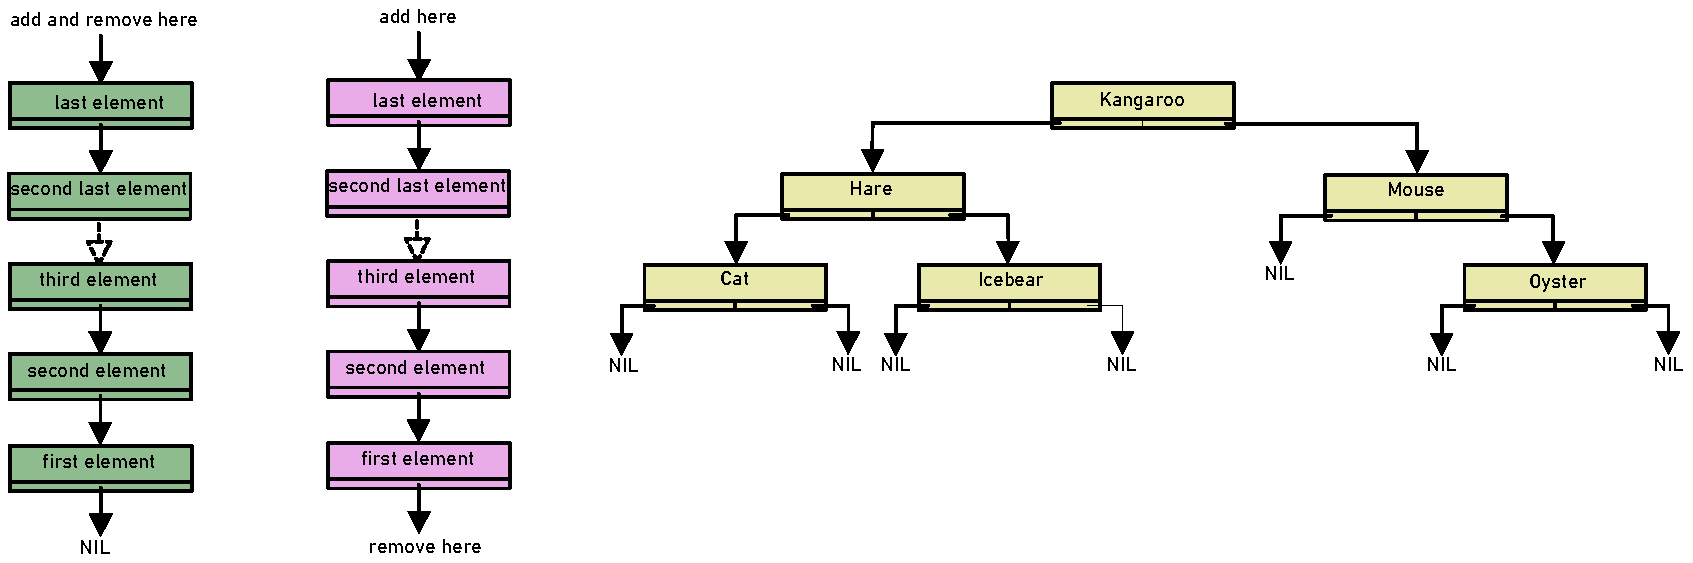
\includegraphics[width=\textwidth]{Graphics/Dynamical}
\end{figure}

This unit provides abstract data structures that can be used to store data of any type (\texttt{procedure Store(var I; S : word);}). The variable \texttt{I} is untyped (more correctly: can have any type). Untyped parameters of functions and procedures were not part of the original \texttt{Pascal}-definitions, they were introduced in \texttt{Turbo-Pascal 4}. From the point of view of this unit, \texttt{I} is simply an \texttt{array [S] of byte}, where \skalar{S} is the number of bytes required (obtained with \texttt{SizeOf()}). This unit was modified from \parencite{Sch-89}. An implementation of abstract binary trees has been published in \parencite{Arb-12}, but isn't needed for this project.

\section{The interface}

\begin{lstlisting}[caption=Interface of unit Dynam]
  UNIT Dynam;

  INTERFACE

  USES MathFunc; // here used only for error handling

  CONST DynamError : BOOLEAN = FALSE;
        MaxElem    = 2000;

  TYPE
    Space = ARRAY[0..MaxElem] OF BYTE;

  { ***************************** LiFo ***************************** }

    LList = ^LListNode;

    LListNode = RECORD
      Size: WORD;
      Info: ^Space;
      Next: LList;
    END;

    LIFO = LList;

  PROCEDURE InitLIFO(VAR L: Lifo);
  {einen leeren Stapel initialisieren}

  FUNCTION EmptyLIFO(L: LIFO): BOOLEAN;
  {pr��fen, ob der Stapel L leer ist}

  PROCEDURE PUSH(VAR L: LIFO; VAR I; S: WORD);
  {einen Wert auf den Stapel legen}

  PROCEDURE POP(VAR L: Lifo; VAR I; S: WORD);
  {einen Wert aus dem Stapel nehmen}

  { ***************************** FiFo ***************************** }

  TYPE
    FList = ^FListNode;

    FListNode = RECORD
      Size: WORD;
      Info: ^Space;
      Next: FList;
    END;

    FIFO = RECORD
      First, last: FList;
    END;

  PROCEDURE InitFIFO(VAR F: FIFO);
  {legt eine leere Schlange an}

  FUNCTION EmptyFIFO(F: FIFO): BOOLEAN;
  {true, wenn die Schlange leer ist}

  PROCEDURE Put(VAR F: FIFO; VAR I; S: WORD);
  {einen Wert I mit Gr��e S in die Schlange schieben}

  PROCEDURE Get(VAR F: FIFO; VAR I; S: WORD);
  {einen Wert I der Gr��e S aus der Schlange holen}

  {****************************************************************************}

  IMPLEMENTATION
  
  VAR ch : char; // for error handling
\end{lstlisting}

\section{The LIFO (stack)}

A LIFO resembles a stack of dinner plates, new plates are added (\texttt{Push}) to the top and also required plates are removed (\texttt{Pop}) from the top (see fig. \ref{fig:Dynam}, \emph{left}). The only two other operations allowed are the creation of a new stack (\texttt{InitLIFO}), and freeing the space of an empty stack (\texttt{EmptyLIFO}).

The items in the stack are linked by pointers. The pointer to the stack points to the top element, which contains a pointer to the next element and so on. When an element is removed from the stack, the pointer to the next element becomes the pointer to the stack; if, on the other hand, an element is added the pointer to the former top becomes its pointer to the next element and the new pointer to the stack points to the new element. At the end of the stack the pointer from the last element (the one added first) is \texttt{NIL}. When the last element has been reached, the pointer to the stack therefore becomes \texttt{NIL}.

\begin{lstlisting}[caption=LIFO]
  PROCEDURE InitLIFO(VAR L: LIFO);


  BEGIN
    L := NIL;
  END; (* InitLIFO *)


  FUNCTION EmptyLIFO(L: LIFO): BOOLEAN;

  BEGIN
    Result := L = NIL;
  END; (* EmptyLIFO *)


  PROCEDURE PUSH(VAR L: LIFO; VAR I; S: WORD);

  VAR
    p: LList;

  BEGIN
    NEW(p);
    WITH p^ DO
      BEGIN
        Size := S;
        Next := L;
        GetMem(Info, Size);
        Move(I, Info^, Size);
      END; (* WITH *)
    L := p;
  END; (* Push *)


  PROCEDURE POP(VAR L: LIFO; VAR I; S: WORD);

  VAR
    p: LList;

  BEGIN
    p := L;
    WITH p^ DO
      BEGIN
        IF Size <> S
          THEN
            BEGIN
              Writeln('TYPE-MISMATCH-ERROR');
              HALT;
            END;
        Move(Info^, I, Size);
        FreeMem(Info, Size);
        L := Next;
      END; (* WITH *)
    DISPOSE(p);
  END; (* Pop *)
\end{lstlisting}

\section{The FIFO (list, buffer, queue)}

If the new mail reaching an office would be added to a \texttt{LIFO}, the mail at the bottom may never be answered.  Therefore, in a queue, the elements are added from one end (\texttt{Put}) and removed from the other (\texttt{Get}). Such a list has two pointers, one for the beginning and the other for the end. The pointer from the element added first is \texttt{NIL} (see fig. \ref{fig:Dynam}, \emph{middle}).

\begin{lstlisting}[caption=FIFO]
  PROCEDURE InitFiFo(VAR F: FiFo);

  BEGIN
    WITH F DO
      BEGIN
        First := NIL;
        last := NIL;
      END;
  END;


  FUNCTION EmptyFiFo(F: FiFo): BOOLEAN;

  BEGIN
    Result := F.First = NIL;
  END;


  PROCEDURE Put(VAR F: FiFo; VAR i; s: WORD);

  VAR p: FList;

  BEGIN
    NEW(p);
    WITH p^ DO
      BEGIN
        Size := S;
        Next := NIL;
        GetMem(Info, Size);
        Move(I, Info^, Size);
      END;
    IF EmptyFiFo(F)
      THEN
        BEGIN
          F.First := p;
          F.last := p;
        END
      ELSE
        BEGIN
          F.last^.Next := p;
          F.last := p;
        END;
  END;


  PROCEDURE Get(VAR F: FiFo; VAR i; s: WORD);

  VAR
    p: FList;

  BEGIN
    p := F.First;
    WITH p^ DO
      BEGIN
        IF Size <> s
          THEN
            BEGIN
              Writeln('Type-Mismatch-Error');
              HALT;
            END;
        Move(Info^, I, Size);
        FreeMem(Info, Size);
        F.First := Next;
      END;
    DISPOSE(p);
  END;
\end{lstlisting}




\section{Test-program}

The following program tests the data structures provided by \texttt{Dynam} and demonstrates how they can be used.

\begin{lstlisting}[caption=Test program]
PROGRAM TestDynam;

USES dynam, mathfunc, crt;


PROCEDURE LifoFifoTesten;

VAR s          : STRING[20];
    LifoListe  : Lifo;
    FifoListe  : Fifo;
    i          : WORD;

BEGIN
  ClrScr;
  Writeln('Demoprogramm f�r die Arbeit mit Fifo und Lifo-Strukturen');
  Writeln;
  InitLifo(LifoListe);
  InitFifo(FifoListe);
  Writeln('Bitte geben Sie jetzt 10 kurze Strings ein (z.B. Namen)');
  Writeln;
  Writeln('EINGABE', 'AUSGABE von LIFO': 30, 'AUSGABE von FIFO': 30);
  Writeln;
  FOR i := 1 TO 10 DO
    BEGIN
      ReadLn(s);
      PUSH(LifoListe, s, SizeOf(s));
      Put(FifoListe, s, SizeOf(s))
    END;
  GotoXY(1, 7);
  WHILE NOT EmptyLifo(LifoListe) DO
    BEGIN
      GotoXY(30, WhereY);
      POP(LifoListe, s, SizeOf(s));
      Writeln(s)
    END;
  GotoXY(1, 7);
  WHILE NOT EmptyFifo(FifoListe) DO
    BEGIN
      GotoXY(60, WhereY);
      Get(FifoListe, s, SizeOf(s));
      Writeln(s)
    END;
  Writeln;
  Writeln('weiter mit RETURN:');
  ReadLn;
END; {LifoFifoTesten}

TYPE KeyType = WORD;

BEGIN  // Test program
  LifoFifoTesten;
END.
\end{lstlisting}

\printbibliography[heading=subbibliography]
\end{refsection}










































































































\part{Univariate statistics}
  \chapter{Statistical distributions}
\begin{refsection}

\abstract{This unit calculates the most important distributions and their integrals. The routines are based on \parencite{Abr-64,Noa-80,Kin-82,Pre-89,PCSig-94}. All probabilities are given in mathematical form, that is in the rage of \(0\ldots 1 \).}

The unit has the following interface:
\begin{lstlisting}[caption=Interface of \texttt{Stat}]
  UNIT Stat;

  INTERFACE

  USES Math, mathfunc;

  CONST
    StatError: BOOLEAN = FALSE;   // toggle FOR error condition

  { **************************** F-distribution **************************** }

  FUNCTION Integral_F(F: float; f1, f2: LONGINT): float;

  FUNCTION Finv( Alpha, Dfn, Dfe: float ) : float;

  { ************************** t-distribution ****************************** }

  FUNCTION Integral_t(t: float; f: LONGINT): float;

  FUNCTION SignificanceLimit_t(p: float; f: LONGINT): float;

  PROCEDURE CompareLiterature(VAR t: float; Average, Sta, Literatur: float;
                              VAR f: LONGINT; n: LONGINT);

  PROCEDURE UnequalSigma(VAR t: float; Average1, Average2, sta1, sta2: float;
                         VAR f: LONGINT; n1, n2: LONGINT);

   { ************************** X2-distribution **************************** }

  FUNCTION IntegralChi(ChiSqr: float; f: WORD): float;

  FUNCTION SignificanceLimit_Chi2 (p : float; dgf : WORD) : float;

  FUNCTION SigChi( Chisq , Df : float ) : float;

  { ***********************  normal distribution *************************** }

  FUNCTION IntegralGauss(z: float): float;

  FUNCTION SignificanceLimitGauss(WantedSecurity: float): float;

  FUNCTION NormalStandardValue (P : float) : float;

  FUNCTION Erf( Z : float ) : float;

  FUNCTION SigNorm (X : float) : float;

  FUNCTION NinvCoarse( P : float ) : float;

  FUNCTION Ninv( P : float ) : float;

  FUNCTION CDNorm (X : float) : float;

  { ********************** binomial distribution *************************** }

  FUNCTION BinominalFrequency (Trials, Success: LONGINT; P: float): float;

  FUNCTION BinominalIntegral (Trials, Value: LONGINT; P: float): float;

  { ************************ Pareto distribution *************************** }

  FUNCTION IntegralPareto (x, Minimum, Shape: float): float;

  FUNCTION PDFPareto (x, Minimum, Shape: float): float;

  { ************************* beta-distribution **************************** }

  FUNCTION CDBeta (X, Alpha, Beta : float; Dprec, MaxIter : INTEGER;
                   VAR Cprec : float; VAR Iter, Ifault : INTEGER  ) : float;

  FUNCTION BetaInv (P, Alpha, Beta : float; MaxIter, Dprec: INTEGER;
                    VAR Iter : INTEGER; VAR Cprec : float; VAR Ierr: INTEGER) : float;

  { ************************* gamma-distribution *************************** }

   FUNCTION ALGama ( Arg : float ) : float;

  FUNCTION GammaInt (Y, P : float; Dprec, MaxIter : INTEGER;
                     VAR Cprec : float; VAR Iter, Ifault  : INTEGER ) : float;

  FUNCTION KolmogorovSmirnovIntegral (alam: float): float;


  IMPLEMENTATION

  CONST Xln2sp   = 0.918938533204673;      // LogE(Sqrt(2 * CONST_PI))
        MaxPrec  = 16;                     // Max. precision
        LnTenInv = 1/Const_ln10;           // 1 / LN(10)

  var ch : char; // for error reporting
\end{lstlisting}

\section{F-distribution}

Integration of the \skalar{F}-distribution gives the probability for the 0-hypothesis that two series of measurements have the same standard deviations. Both series must be normally distributed and free of outliers.

\begin{lstlisting}[caption=Routines for the F-Distribution]
  FUNCTION Integral_F(F: float; f1, f2: LONGINT): float;

  VAR
    S, X, A, B, V: float;


    FUNCTION R0(M, N: LONGINT; V: float): float;

    VAR
      G, Sum: float;
      k, TEST: LONGINT;

    BEGIN
      k := 1;
      G := 1;
      Sum := G;
      TEST := M DIV 2;
      WHILE NOT (k = TEST) DO
        BEGIN
          k := Succ(k);
          G := G * V * (N + 2 * k - 4) / (2 * k - 2);
          Sum := Sum + G;
        END;
      Integral_F := Sum;
    END;


    FUNCTION R1(M: LONGINT; V: float): float;

    VAR
      G, Sum: float;
      k, TEST: LONGINT;

    BEGIN
      k := 1;
      G := Sqrt(V);
      Sum := G;
      TEST := (M - 1) DIV 2;
      WHILE NOT (k = TEST) DO
        BEGIN
          k := Succ(k);
          G := G * V * (2 * k - 2) / (2 * k - 1);
          Sum := Sum + G;
        END;
      R1 := Sum;
    END;


    FUNCTION R2(f1, f2: LONGINT; V: float): float;

    VAR
      G, Sum: float;
      k, TEST: LONGINT;

    BEGIN
      k := 1;
      G := 1;
      Sum := G;
      TEST := (f1 - 1) DIV 2;
      WHILE NOT (k = TEST) DO
        BEGIN
          k := Succ(k);
          G := G * V * (f2 + 2 * k - 3) / (2 * k - 1);
          Sum := Sum + G;
        END;
      R2 := Sum;
    END;


    FUNCTION Q(f2: LONGINT): float;

    VAR
      k: LONGINT;
      Product: float;

    BEGIN
      Product := 1;
      FOR k := 1 TO ((f2 - 1) DIV 2) DO
        Product := Product * (k / (k - 0.5));
      Q := (2 / Pi) * Product;
    END;

  BEGIN
    IF (f1 MOD 2) = 0
      THEN
        BEGIN
          X := f2 / (f2 + f1 * F);
          S := 1 - (R0(f1, f2, 1 - x) * Pot(X, f2 / 2));
        END
      ELSE IF (f2 MOD 2) = 0
             THEN
               BEGIN
                 X := f2 / (f2 + f1 * F);
                 S := Pot(1 - x, f1 / 2) * R0(f2, f1, X);
               END
             ELSE IF (f1 = 1) AND (f2 = 1)
                    THEN
                      S := (2 / Pi) * ArcTan(Sqrt(F))
                    ELSE IF (f1 = 1) AND (f2 > 1)
                      THEN
                        BEGIN
                          X := Sqrt(F / f2);
                          V := 1 / (1 + Sqr(X));
                          S := (2 / Pi) * (ArcTan(X) + X * R1(f2, V) * Sqrt(1 / (1 + Sqr(X))));
                        END
                      ELSE IF (f1 > 1) AND (f2 = 1)
                             THEN
                               BEGIN
                                 X := Sqrt(1 / (f1 * F));
                                 V := 1 / (1 + Sqr(X));
                                 S := 1 - (2 / Pi) * (ArcTan(X) + X * R1(f1, V) *
                                      Sqrt(1 / (1 + Sqr(X))));
                               END
                             ELSE           {f1 und f2 ungerade und > 1}
                               BEGIN
                                 X := Sqrt(F * f1 / f2);
                                 V := 1 / (1 + Sqr(X));
                                 A := (2 / Pi) * (ArcTan(X) + X * R1(f2, V) *
                                   Sqrt(1 / (1 + Sqr(X))));
                                 V := Sqr(X) / (1 + Sqr(X));
                                 B := Q(f2) * X * Pot(1 / (1 + Sqr(X)), (f2 + 1) / 2) *
                                   R2(f1, f2, V);
                                 S := A - B;
                               END;
    Result := 1 - S;
  END;    // Integral_F


  FUNCTION Finv( Alpha, Dfn, Dfe: float ) : float;

  CONST MaxIter  = 100;
        Dprec    = 10;

  VAR Fin, Cprec : float;
      Iter, Ierr : INTEGER;

  BEGIN
    Fin   := -1.0;
    IF ((Dfn > 0.0) AND (Dfe > 0.0))
      THEN
        IF ((Alpha >= 0.0) AND (Alpha <= 1.0))
          THEN
            BEGIN
              Fin := BetaInv(1.0 - Alpha, Dfn/2.0, Dfe/2.0, MaxIter, Dprec,
                             Iter, Cprec, Ierr);
              IF ((Fin >= 0.0) AND (Fin < 1.0) AND (Ierr = 0))
                THEN Fin := Fin * Dfe / (Dfn * (1.0 - Fin));
            END;
    Finv := Fin;
  END   (* Finv *);
\end{lstlisting}

\section{\Name{Student}'s t-distribution}

Integration of the \skalar{t}-distribution returns the error probability for a given \skalar{t} and degree of freedom \skalar{f}:

\begin{lstlisting}[caption=Routines for t-distribution]
  FUNCTION Integral_t(t: float; f: LONGINT): float;

  VAR
    x, u, v, w: float;


    FUNCTION R(f, v, w: float): float;

    VAR
      g, Sum: float;
      i: LONGINT;

    BEGIN
      i := 2;
      Sum := w;
      g := w;
      REPEAT
        g := g * v * (i / (i + 1));
        Sum := Sum + g;
        i := i + 2;
      UNTIL i > (f - 3);
      R := Sum;
    END;


    FUNCTION Q(f, v: float): float;

    VAR
      g, Sum: float;
      i: LONGINT;

    BEGIN
      Sum := 1;
      i := 1;
      g := 1;
      REPEAT
        g := g * v * (i / (i + 1));
        Sum := Sum + g;
        i := i + 2;
      UNTIL i > (f - 3);
      Q := Sum;
    END;

  BEGIN
    x := t / Sqrt(f);
    IF f = 1
      THEN
        u := 2 / Pi * ArcTan(x)
      ELSE
        BEGIN
          v := 1 / (1 + Sqr(x));
          IF Odd(f)
            THEN
              BEGIN
                w := Sqrt(v);
                u := 2 / Pi * (R(f, v, w) * Sqrt(1 - v) + ArcTan(x));
              END
            ELSE
              u := Q(f, v) * Sqrt(1 - v);
        END;
    Result := 1 - u;
  END;  // Integral_t
\end{lstlisting}

\texttt{SignificanceLimit\_t} returns that \skalar{t}-value where the error probability becomes lower than a given value:

\begin{lstlisting}[caption=]
  FUNCTION SignificanceLimit_t(p: float; f: LONGINT): float;

  CONST
    a0 = 2.515517;      a1 = 0.802853;      a2 = 0.010328;
    b1 = 1.432788;      b2 = 0.189269;      b3 = 0.001308;

  VAR
    s, q, n, z, d, t1, t2, t4, a, b, c, x: float;

  BEGIN
    s := 1 - p;
    q := p / 2;
    n := Sqrt(Ln(1 / Sqr(q)));
    z := n - (a0 + n * (a1 + a2 * n)) / (1 + n * (b1 + n * (b2 + b3 * n)));
    d := Ln(z);
    t1 := tan(Pi * s / 2);
    t2 := Sqrt(2 * (1 / (1 - Sqr(s)) - 1));
    t4 := 2 * Sqrt(1 / (2 * Cos(ArcCos(1 - 2 * Sqr(s)) / 3) - 1) - 1);
    a := (Ln(t1) - 6 * Ln(t2) + 8 * Ln(t4) - 3 * d) / 0.375;
    b := 2 * Ln(t1) - 4 * Ln(t2) + 2 * d - 3 * a / 2;
    c := Ln(t1) - d - a - b;
    x := 1 / f;
    Result := Exp(d + x * (c + x * (b + a * x)));
  END;   // SignificanceLimit_t
\end{lstlisting}

\subsection{Calculating \skalar{t}}

The \skalar{t}-test is used to compare two values. The samples should be either normally distributed or large enough that the central limit theorem applies (\( > 30 \)). Their variance is unknown, otherwise a \Name{Gauss}-test would be more appropriate. That is, instead of \[ Z = \sqrt{n} \frac{\bar{\AbsVec{x}} - \mu_0}{\sigma} \], which is normally distributed, we use \[ T = \sqrt{n} \frac{\bar{\AbsVec{x}} - \mu_0}{S} \], which is \skalar{t}-distributed, as test-statistics. The distribution was developed by \Name{William Sealy Gosset}, who published under the pseudonym \Name{Student} \parencite{Stu-08}.

\subsubsection{One-sample \skalar{t}-test}

If there is only one data vector \AbsVec{x}, whose average is to be compared with a population mean, literature value or desired value \skalar{\mu_0}, then \( \mathbf{H_0}: \bar{\AbsVec{x}} = \mu_0 \) (two-sided test, or larger or smaller for a one-sided test):
\begin{eqnarray}
  \nonumber % Remove numbering (before each equation)
  \nu     &=& n - 1 \\
  \hat{t} &=& \sqrt{n} \frac{\bar{\AbsVec{x}} - \mu_0}{s}
\end{eqnarray}

The test is
\begin{description}
  \item[right-sided]{\( \mathbf{H}_0: \bar{\AbsVec{x}} \leq \mu_0 \), rejected with probability \skalar{\alpha} if  \( \hat{t} > t_{1-\alpha, \nu}  \)}
  \item[two-sided]{\( \mathbf{H}_0: \bar{\AbsVec{x}}  = \mu_0 \), rejected with probability \skalar{\alpha} if  \( |\hat{t}| > t_{1-\frac{\alpha}{2}, \nu} \)}
  \item[left-sided]{\( \mathbf{H}_0: \bar{\AbsVec{x}}  \geq \mu_0 \), rejected with probability \skalar{\alpha} if  \( \hat{t} < t_{1-\alpha, \nu}  \)}
\end{description}


\begin{lstlisting}[caption=t for comparing sample with population]
  PROCEDURE CompareLiterature(VAR t: float; Average, sta, literatur: float;
    VAR f: LONGINT; n: LONGINT);

  BEGIN
    t := (Abs(Average - literatur) / sta) * Sqrt(n);
    f := n - 1;
  END;
\end{lstlisting}

\subsubsection{Paired two samples}

If there are two samples, but those are paired (\Foreign{e.g.}, right and left arm of the same person, or values of the same person obtained before and after treatment), then we can test the average of their differences against zero, this is more powerful than doing a two-sample test.

\subsubsection{The two-sample \skalar{t}-test with equal variances}

The two-sample \skalar{t}-test is used to compare the difference of two averages \skalar{\bar{\AbsVec{x}}_1, \bar{\AbsVec{x}}_2} with the null-hypothesis
\begin{description}
  \item[right-sided]{\( \mathbf{H}_0: \bar{\AbsVec{x}}_1 - \bar{\AbsVec{x}}_2  \leq\ \omega_0 \)}
  \item[two-sided]{\( \mathbf{H}_0: \bar{\AbsVec{x}}_1 - \bar{\AbsVec{x}}_2  = \omega_0 \)}
  \item[left-sided]{\( \mathbf{H}_0: \bar{\AbsVec{x}}_1 - \bar{\AbsVec{x}}_2  \geq \omega_0 \)}
\end{description}
, where \skalar{\omega_0} is the assumed difference between the averages (usually zero).

In case both samples are independent, but have identical variance, \skalar{t} and \skalar{\nu} are calculated by
\begin{eqnarray}
  \nonumber
  \nu &=& n_1 + n_2 - 2 \\
  \nonumber
  s^* &=& \sqrt{\frac{(n_1 - 1) s_1^2 (n_2 - 1) s_2^2}{\nu}} \\
  t &=& \frac{\bar{\AbsVec{x}}_1 - \bar{\AbsVec{x}}_2 - \omega_0}{s^* \sqrt{\frac{1}{n_1}+\frac{1}{n_2}}} = \sqrt{\frac{n_1 n_2}{n_1 + n_2}} \frac{\bar{\AbsVec{x}}_1 - \bar{\AbsVec{x}}_2 - \omega_0}{s^*}
\end{eqnarray}
with \skalar{s^*} the pooled (weighted) standard deviation of both samples.

\begin{lstlisting}[caption=t for independent samples of equal variance]
  PROCEDURE EqualSigma(VAR t: float; Average1, Average2, sta1, sta2: float;
    VAR f: LONGINT; n1, n2: LONGINT);

  VAR
    sta: float;

  BEGIN
    f := n1 + n2 - 2;
    sta := Sqrt((n1 - 1) * Sqr(sta1) + (n2 - 1) * Sqr(sta2) / f);
    t := (Abs(Average1 - Average2) / sta) * Sqrt(n1 * n2 / (n1 + n2));
  END;
\end{lstlisting}

\subsubsection{The two-sample \skalar{t}-test with unequal variances (\Name{Welch}-test)}

In case the samples are independent, and have unequal variance, then:
\begin{eqnarray}
  \nonumber
  \nu &=& \frac{\left( \frac{s_1^2}{n_1} + \frac{s_2^2}{n_2} \right)^2}{\frac{\left( \frac{s_1^2}{n_1} \right)^2}{n_1 - 1} + \frac{\left( \frac{s_2^2}{n_2} \right)^2}{n_2 - 1}}\\
  \nonumber
  s^* &=& \sqrt{\frac{s_1^2}{n_1} + \frac{s_2^2}{n_2}} \\
  t &=& \frac{\bar{\AbsVec{x}}_1 - \bar{\AbsVec{x}}_2 - \omega_0}{s^*}
\end{eqnarray}

\begin{lstlisting}[caption=t for independent samples of unequal variance]
  PROCEDURE UnequalSigma(VAR t: float; Average1, Average2, sta1, sta2: float;
    VAR f: LONGINT; n1, n2: LONGINT);

  BEGIN
    t := Abs(Average1 - Average2) / (Sqrt(Sqr(sta1) / n1) + Sqrt(Sqr(sta2) / n2));
    f := Round((Sqr(Sqr(sta1) / n1 + Sqr(sta2) / n2) /
      (Sqr(Sqr(sta1) / n1) / (n1 + 1) + Sqr(Sqr(sta2) / n2) / (n2 - 1))) - 2);
  END;
\end{lstlisting}


\section{ \( \chi^2 \) Distribution}\label{text:chi2}

\( \chi^2 \) is defined as
\begin{equation}
   \chi^2 = \sum_{i=1}^{n}{\frac{(O_i - E_i)^2}{E_i}}
\end{equation}
where \skalar{O} and \skalar{E} are the observed and expected values, under the condition that \( E_i > 0\ \forall\ i \), and that \( \sum_{i=1}^{n}{O_i} = \sum_{i=1}^{n}{E_i} = n \) \parencite{Hel-76}.

The integral of the \(\chi^2 \)-distribution is calculated by \parencite[Eqn 26.4.6]{Abr-64} which, however, causes an overflow for \(\chi^2 > 550 \) or so. Therefore, for \(\chi^2 > 500 \) the integral is calculated as described in
\parencite[p. 526]{Pre-89}. The latter method, however, doesn't converges if \(P_0 > \SI{20}{\%} \) or so.

\begin{lstlisting}[caption= \( \chi^2 \) Distribution]
  UNCTION IntegralChi(chisqr: float; f: WORD): float;

  VAR
    s1, s2, s3: extended;
    c: CHAR;

    FUNCTION Reihe1(chi: extended; f: WORD): float;

    VAR
      Fraction, Sum, Summand: extended;
      k, i: LONGINT;

    BEGIN
      Sum := 1;
      k := 1;
      REPEAT
        Fraction := 1;
        FOR i := 1 TO k DO
          Fraction := Fraction * (f + 2 * i);
        Summand := Exp(Ln(chi) * 2 * k) / Fraction;
        Sum := Sum + Summand;
        INC(k);
      UNTIL (Summand < MaxError);             {gewünschte Genauigkeit}
      Result := Sum;
    END;

  BEGIN
    IF Abs(ChiSqr) < Zero           // chi^2 ~ 0
    THEN
    BEGIN
      Result := 0.0;
      EXIT;
    END;
    IF ChiSqr < 0                   // should NOT happen
    THEN
      BEGIN
        Result := NaN;
        c := WriteErrorMessage('Integral of chi^2: chi^2 < 0');
        StatError := TRUE;
        EXIT;
      END;
    IF ChiSqr < 500
      THEN
        BEGIN                       // formula 26.4.6 OF Abramowitz & Stegun
          s1 := f / 2 * Ln(chisqr / 2);
          s2 := Ln(Reihe1(Sqrt(chisqr), f));
          s3 := ((-chisqr / 2) - LnGamma((f + 2) / 2));
          Result := 1 - Exp(s1 + s2 + s3);
        END
      ELSE
        BEGIN                      // page 526 OF Numerical Methods
          Result := IncompleteGamma(0.5 * f, 0.5 * ChiSqr);
          IF MathError
            THEN                   // no convergence
              BEGIN
                Result := NaN;
                MathError := FALSE;
                StatError := TRUE;
                c := WriteErrorMessage('Integral Chi-Sqr: no convergence');
              END;
        END;
  END;
\end{lstlisting}

The following function calculates the error probability given \skalar{\chi^2} and \skalar{\nu} by transforming the input data to match the requirements of the \textGamma-distribution. Function \texttt{GammaInt} then provides the corresponding cumulative incomplete \textGamma-probability. An error in the input arguments results in a returned
probability of -1.

\begin{lstlisting}[caption=Alternative \( \chi^2 \) integral]
  FUNCTION SigChi( Chisq , Df : float ) : float;

  CONST MaxIter = 200;
        Dprec   = 12;

  VAR Ierr, Iter : INTEGER;
     Cprec       : float;

  BEGIN
     SigChi := 1.0 - GammaInt(Chisq / 2.0, Df / 2.0, Dprec, MaxIter, Cprec, Iter, Ierr);
     IF ( Ierr <> 0 ) THEN SigChi := -1.0;
  END   (* SigChi *);
\end{lstlisting}

\subsubsection{The inverse \skalar{\chi^2} distribution}

\begin{figure}
 \caption{\capstart \skalar{h_{60}}-values as function of \skalar{P}.  }
 \label{fig:h60}
 \centering
 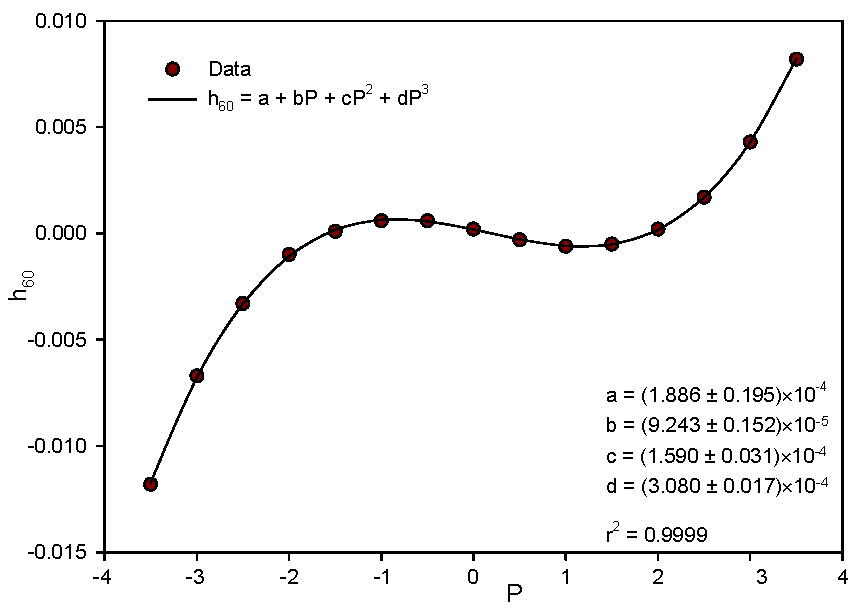
\includegraphics[width=0.75\textwidth]{Graphics/h60}
\end{figure}

Sometimes we have a desired probability for a given degree of freedom, and want to know how high the corresponding \skalar{\chi^2} needs to be. \parencite{Lia-68} gives three approximation, quadratic, cubic and improved cubic. Of these, the cubic is the most accurate for \( \nu \leq 10 \), and the improved cubic for \( \nu > 10 \):
\begin{equation}
  \chi^2(P|\nu) = \left\{
          \begin{array}{l@{\;}l}
             \nu \left[1 - \frac{2}{9 \nu}  + x_p \sqrt{\frac{2}{9 \nu}}\right]^3                           & \quad \forall \nu \leq 10  \\
             \nu \left[1 - \frac{2}{9 \nu} + (x_p - \frac{60 h(x_P)}{\nu}) \sqrt{\frac{2}{9 \nu}}\right]^3  & \quad \forall \nu > 10 \\
          \end{array}
        \right.
\end{equation}
The paper has a table of \skalar{h(x_P)}-values, but as can be seen in fig. \ref{fig:h60}, these can bee fitted very well with a polynom of 3rd order. \skalar{x_p} is such that the standardised normal probability function \( P(x_p) = 1 - P \).

\begin{lstlisting}[caption= \( \chi^2 \) required]
  FUNCTION SignificanceLimit_Chi2 (p : float; dgf : WORD) : float;

     FUNCTION H (x : float) : float;

     CONST a = 1.886e-4; b = 9.243e-5; c = 1.590e-4; d = 3.080e-4;

     BEGIN
       Result := a + b*x + c*x*x + d*x*x*x;
     END;

  VAR x, y : float;

  BEGIN
    y := -NormalStandardValue(p);
    IF dgf <= 10
      THEN x := (1 - 2/(9*dgf) + y                   * Sqrt(2/(9*dgf)))
      ELSE x := (1 - 2/(9*dgf) + (y - (h(y)*60/dgf)) * Sqrt(2/(9*dgf)));
    Result := dgf * x*x*x;
  END;
\end{lstlisting}

\subsection{The \skalar{G}-distribution}

The \skalar{G}-distribution \parencite{Sok-81} is related to the \skalar{\chi^2}-distribution and defined as
\begin{equation}
  G = 2 \sum_{i=1}^{n}{O_i \ln\left( \frac{O_i}{E_i} \right)}
\end{equation}
under the same conditions as for \skalar{\chi^2}. \skalar{G} follows a \skalar{\chi^2}-distribution with the same degrees of freedom, however, when used for small \skalar{n}, \skalar{G} approximates better than \Name{Pearson}'s \skalar{\chi^2}.

\section{\Name{Gauss}' normal distribution}

A continuous random variable \skalar{x \in \set{R}} is \Name{Gauss}ian normal distributed with mean \skalar{\mu} and variance \skalar{\sigma^2} (\( x \sim N(\mu, \sigma^2) \)), if \skalar{x} has the following probability density:
\begin{equation}
  f(x | \mu, \sigma^2) = \frac{1}{\sqrt{2\pi\sigma^2}} \exp\left( -\frac{(x-\mu)^2}{2\sigma^2} \right)
\end{equation}
This function has a bell-shaped, symmetrical  graph where \skalar{\mu} is the centre of symmetry and also the median and modus. \skalar{\mu\pm\sigma} are the inflexion points. The \textbf{standard normal distribution} has \( \mu = 0, \sigma^2 = 1\).

The integral of the \Name{Gauss}-distribution is:
\begin{equation}
  F(x | \mu, \sigma^2) = \frac{1}{\sqrt{2\pi}\sigma} \int_{-\infty}^{x} \exp\left[ -\frac{1}{2}\left(\frac{t-\mu}{\sigma}\right) \right] \mathrm{d}t
\end{equation}
Then for integration between
\begin{description}
  \item[ \( z1\ldots z2 \)]{\hspace{10mm}
     \begin{description}
        \item[\( z1 < 0 \) and \(z2 < 0 \)]{\( w = 0.5 * (\mathrm{GI}(\abs(z1)) - \mathrm{GI}(\abs(z2))) \)}
        \item[\( z1 > 0 \) and \(z2 > 0 \)]{\( w = 0.5 * (\mathrm{GI}(z1) + \mathrm{GI}(z2)) \)}
        \item[\( z1 < 0 \) and \(z2 > 0 \)]{\( w = 0.5 * (\mathrm{GI}(\abs(z1))) + \mathrm{GI}(z2) \)}
     \end{description}  }
  \item[\( -\infty\ldots z \)]{\hspace{10mm}
     \begin{description}
        \item[\( z > 0 \)]{\( w = 0.5 + 0.5 * \mathrm{GI}(z) \)}
        \item[\( z < 0 \)]{\( w = 0.5 - 0.5 * \mathrm{GI}(\abs(z)) \)}
     \end{description} }
  \item[ \( z\ldots \infty \)]{\hspace{10mm}
     \begin{description}
        \item[\( z > 0 \)]{\( w = 0.5 - 0.5 * \mathrm{GI}(z) \)}
        \item[\( z < 0 \)]{\( w = 0.5 + 0.5 * \mathrm{GI}(\abs(z)) \)}
     \end{description} }
\end{description}
The \textbf{central limit theorem} of \Name{Lindeberg \& Lévy} states, that the sum of (infinitely) many random variables is normally distributed, as long as none of the individual variables exerts a dominating influence on \skalar{\sigma}. Since  variables in nature are often determined by many interacting causes, the normal distribution is very common.

\begin{lstlisting}
  FUNCTION IntegralGauss(z: float): float;

  VAR
    f: float;


    FUNCTION Reihe(z: float): float;

    VAR
      Sum, G: float;
      i: INTEGER;

    BEGIN
      Sum := z;
      i := 1;
      G := z;
      REPEAT
        G := G * Sqr(z) / (2 * i + 1);
        INC(i);
        Sum := Sum + G;
      UNTIL G < MaxError;
      Result := Sum;
    END;

  BEGIN
    f := Exp(-Sqr(z) / 2) / Sqrt(2 * Pi);
    IntegralGauss := 2 * f * Reihe(z);
  END;
\end{lstlisting}

The next function calculates the factor with which the standard deviation needs to be multiplied so that any measured value is with a wanted probability in \(-nz\ldots +nz \):

\begin{lstlisting}[caption=]
  FUNCTION SignificanceLimitGauss(WantedSecurity: float): float;
  // -z ... z

  CONST
    a0 = 2.515517;    a1 = 0.802853;    a2 = 0.010328;
    b1 = 1.432788;    b2 = 0.189269;    b3 = 0.001308;

  VAR
    p, q, n, z0, f, p0, t: float;


    FUNCTION Reihe(z: float): float;

    VAR
      Sum, G: float;
      i: INTEGER;

    BEGIN
      Sum := z;
      i := 1;
      G := z;
      REPEAT
        G := G * Sqr(z) / (2 * i + 1);
        INC(i);
        Sum := Sum + G;
      UNTIL G < MaxError;
      Result := Sum;
    END;

  BEGIN
    q := (1 - WantedSecurity) / 2;
    p := 1 - q;
    n := Sqrt(Ln(1 / Sqr(q)));
    z0 := n - (a0 + n * (a1 + a2 * n)) / (1 + n * (b1 + n * (b2 + b3 * n)));
    f := Exp(-Sqr(z0) / 2) / Sqrt(2 * Pi);
    p0 := 0.5 + f * Reihe(z0);
    t := (p - p0) / f;
    Result := z0 + t + z0 * Sqr(t) / 2 + (2 * Sqr(z0) + 1) / 6 * pot(t, 3);
  END;
\end{lstlisting}


The next function calculates the factor with which the standard deviation needs to be multiplied so that any measured value is with a wanted probability in \(-\infty\ldots +nz \). It is based on \parencite{Vou-10}.

\begin{lstlisting}[caption=Normal standard value]
  FUNCTION NormalStandardValue (P : float) : float;

  CONST a0 = 0.389422403767615;     a1 = -1.699385796345221; a2 = 1.246899760652504;
        b0 = 0.155331081623168;     b1 = -0.839293158122257;
        c0 = 16.896201479841517652; c1 = -2.793522347562718412;
        c2 = -8.731478129786263127; c3 = -1.000182518730158122;
        d0 = 7.173787663925508066;  d1 = 8.759693508958633869;

  VAR q, r : float;
      c    : CHAR;

  BEGIN
    IF (P < 1e-298) OR (P > (1-1e-298))
      THEN
        BEGIN
          c := WriteErrorMessage('Normal standard value: Value outside range');
          Result := NaN;
          StatError := TRUE;
          EXIT;
        END;
    IF P < 0.0465
      THEN  // lower tail
        BEGIN
          r := Sqrt(Ln(1/(P*P)));
          Result := (c0 + c1*r + c2*r*r + c3*r*r*r) / (d0 + d1*r + r*r);
        END
      ELSE
        IF P < 0.9535
          THEN  // central region
            BEGIN
              q := p-0.5;
              r := q*q;
              Result := q * (a0 + a1*r + a2*r*r) / (b0 + b1*r + r*r);
            END
          ELSE  // upper tail
            BEGIN
              q := 1-p;
              r := Sqrt(Ln(1/(q*q)));
              Result := -(c0 + c1*r + c2*r*r + c3*r*r*r) / (d0 + d1*r + r*r);
            END;
  END;
\end{lstlisting}

The \Name{Gauss}ian error function is
\begin{equation}
   \mathrm{erf}(x) = \frac{2}{\sqrt{\pi}} \int_{0}^{x} \mathrm{e}^{-r^2} \mathrm{d}r \approx \frac{2}{\sqrt{\pi}} \sum_{n=0}^{\infty} \frac{(-1)^n x^{2n + 1}}{(2n + 1) n!}
 \end{equation}
, which for \( x \in \set{R} \) returns real numbers in \( [-1\ldots +1] \). The generalisation to complex arguments is of no interest here. The conjugated error function is
\begin{equation}
  \mathrm{erfc} (x) = \frac{2}{\sqrt{\pi}} \int_{x}^{\infty} \mathrm{e}^{-r^2} \mathrm{d}r = 1 - \mathrm{erf}(x)
\end{equation}

\begin{lstlisting}[caption=Error function]
  FUNCTION Erf (Z : float) : float;

  CONST A:  ARRAY[1..14] OF float =
            ( 1.1283791670955,       0.34197505591854,     0.86290601455206E-1,
              0.12382023274723E-1,   0.11986242418302E-2,  0.76537302607825E-4,
              0.25365482058342E-5,  -0.99999707603738,    -1.4731794832805,
             -1.0573449601594,      -0.44078839213875,    -0.10684197950781,
             -0.12636031836273E-1,  -0.1149393366616E-8  );

        B:  ARRAY[1..12] OF REAL =
            ( -0.36359916427762,     0.52205830591727E-1, -0.30613035688519E-2,
              -0.46856639020338E-4,  0.15601995561434E-4, -0.62143556409287E-6,
               2.6015349994799,      2.9929556755308,      1.9684584582884,
               0.79250795276064,     0.18937020051337,     0.22396882835053E-1 );

  VAR U, X, S:  float;

  BEGIN
    X := ABS(Z);                 (* Get absolute value of argument *)
    S := Signum(Z);              (* Remember sign of argument *)
    IF ( S = 0.0 )               (* Check for zero argument *)
      THEN
        Result := 0.0
      ELSE                       (* Check for large argument *)
        IF (X >= 5.5)
          THEN
            Result := S
          ELSE                   (* Arg in approximation range *)
            BEGIN
                U := X * X;
                IF (X <= 1.5)
                  THEN           (* Approx. for arg <= 1.5 *)
                    Result := (X * EXP(-U) * (A[1] + U * (A[2] + U *
                              (A[3] + U * (A[4] + U * (A[5] + U *
                              (A[6] + U * A[7] )))))) /
                              (1.0 + U * (B[1] + U * (B[2] + U *
                              (B[3] + U * (B[4] + U * (B[5] + U *
                              B[6] ))))))) * S
                  ELSE          (* Approx. for arg > 1.5 *)
                    Result := (EXP(-U) * (A[8] + X * (A[9] + X * (A[10] + X *
                              (A[11] + X * (A[12] + X * (A[13] + X * A[14] )))))) /
                              (1.0 + X * (B[7] + X * (B[8] + X * (B[9] + X *
                              (B[10] + X * (B[11] + X * B[12])))))) + 1.0) * S;
            END;
  END;   (* Erf *)
\end{lstlisting}

The error function is related to the normal distribution with standard deviation \skalar{\sigma} and expected value \skalar{\mu}
\begin{equation}
  F(x) = \frac{1}{2} \left[ 1 + \mathrm{erf}\left( \frac{x-\mu}{\sigma \sqrt{2}} \right) \right]
\end{equation}

\begin{lstlisting}[caption=Tail probability of normal distribution]
  FUNCTION SigNorm (X : float) : float;

  BEGIN
      IF X >= 0.0
        THEN Result := 1.0 - (1.0 + Erf(X / Const_Sqrt2)) / 2.0
        ELSE Result := 1.0 - (1.0 - Erf(-X / Const_Sqrt2)) / 2.0;
  END   (* SigNorm *);
\end{lstlisting}

\begin{lstlisting}[caption=Cumulative normal distribution probability]
  FUNCTION CDNorm (X : float) : float;

  BEGIN
     IF X >= 0.0
       THEN Result := ( 1.0 + Erf(  X / Const_Sqrt2 ) ) / 2.0
       ELSE Result := ( 1.0 - Erf( -X / Const_Sqrt2 ) ) / 2.0;
  END;
\end{lstlisting}

An alternative way to calculate the percentage point of the normal distribution with about \num{6} valid figures is
\begin{lstlisting}[caption=percentage point of normal distribution]
  FUNCTION NinvCoarse (P : float) : float;

  CONST Lim = 1.0E-20;

  VAR Y :  float;
      Pr: float;
      Nv: float;

  CONST PN : ARRAY [1..5] OF float =
             ( -0.322232431088  ,  -1.0              , -0.342242088547  ,
               -0.0204231210245 ,  -0.453642210148E-4 );

         QN : ARRAY [1..5] OF float =
             ( 0.0993484626060 ,    0.588581570495   ,  0.531103462366  ,
               0.103537752850  ,    0.38560700634E-2  );

  BEGIN (* NinvCoarse *)
    Result := 0.0;
    IF (P > 0.5)
      THEN Pr := 1.0 - P
      ELSE Pr := P;
    IF (( Pr >= Lim ) AND ( Pr <> 0.5 ))
      THEN
        BEGIN
          Y := SQRT ( LN( 1.0 / Pr / Pr ) );
          Nv := Y + ((((Y * PN[ 5 ] + PN[ 4 ]) * Y + PN[ 3 ] ) * Y
                                    + PN[ 2 ]) * Y + PN[ 1 ] ) /
                    ((((Y * QN[ 5 ] + QN[ 4 ]) * Y + QN[ 3 ] ) * Y
                                    + QN[ 2 ]) * Y + QN[ 1 ] );
          IF (P < 0.5)
            THEN Result := -Nv
           ELSE Result := Nv;
        END;
  END   (* NinvCoarse *);
\end{lstlisting}
This result can be made precise to \num{12} valid figures by using a \Name{Taylor} series on the approximation error:
\begin{lstlisting}[caption=percentage point of normal distribution]
  FUNCTION Ninv( P : float ) : float;

  VAR Xp, P1, Z, X3, X2, X1, Phi: float;

  BEGIN
    Xp := Ninv(P);
    P1 := SigNorm(Xp);
    Phi := SQRT(1.0 / (2.0 * PI)) * EXP(-(Xp * Xp) / 2.0);
    Z  := (P - P1) / Phi;
    X3 := (2.0 * (Xp * Xp) + 1.0) * Z / 3.0;
    X2 := (X3 + Xp) * Z / 2.0;
    X1 := ((X2 + 1.0) * Z);
    Result := Xp + X1;
  END   (* Ninv *);
\end{lstlisting}


\section{Binomial distribution}

The binomial frequency is the probability to have \texttt{Success} successes out of \texttt{trials} attempts, when the success probability per attempt is \skalar{P}

\begin{lstlisting}[caption=Routines for the binomial distribution]
  FUNCTION BinominalFrequency(Trials, Success: LONGINT; P: float): float;

  VAR
    TrialsOverSuccess: float;

  BEGIN
    TrialsOverSuccess := BinomialCoef(Trials, Success);
    Result := TrialsOverSuccess * pot(P, Success) *
      pot(1 - P, Trials - Success);
  END;
\end{lstlisting}

The integral is the probability that the number of successes is less or equal than \texttt{Value}, when the number of trials is \texttt{Trials} and the probability of success in each trial is \skalar{P}.

\begin{lstlisting}[caption=]
  FUNCTION BinominalIntegral(Trials, Value: LONGINT; P: float): float;

  VAR
    Sum: float;
    i: WORD;

  BEGIN
    Sum := 0.0;
    FOR i := 0 TO Value DO
      Sum := Sum + BinominalFrequency(Trials, i, P);
    Result := Sum;
  END;
\end{lstlisting}

\section{The \Name{Pareto} (80/20) distribution}

The \Name{Pareto} distribution \parencite{Par-87} describes a continuous function on the interval \([x_\mathrm{min}, \infty]\), the cumulative distribution function of the \Name{Pareto}-distribution with Minimum \(x_\mathrm{min} \geq 0 \), Shape \(k > 1 \) is
\begin{equation}
  f(x) = \left\{
     \begin{array}{lr}
         \frac{k x_\mathrm{min}^k}{x^{k+1}} & x \geq x_\mathrm{min} \\
         0                                  & x < x_\mathrm{min}
     \end{array}
  \right.
\end{equation}
This distribution can describe parameters that cover several orders of magnitude and depend on many random factors. The \Name{Pareto}-principle says that the lowest \SI{20}{\%} of the independent variable account for \SI{80}{\%} of the dependent variable (law of diminishing return), then \(k \approx\ 1.16\).


\begin{lstlisting}[caption=The \Name{Pareto} distribution]
  FUNCTION IntegralPareto(x, Minimum, Shape: float): float;

  BEGIN
    Result := 1 - Pot((Minimum / x), Shape);
  END;


  FUNCTION ProbabilityDistributionFunctionPareto(x, Minimum, Shape: float): float;

  BEGIN
    Result := Shape * pot(Minimum, Shape) / pot(x, Shape + 1);
  END;


  END.  // Stat
\end{lstlisting}

\section{The \textbeta-distribution}

\begin{lstlisting}[caption=\textbeta distribution]
  FUNCTION CDBeta (X, Alpha, Beta : float; Dprec, MaxIter : INTEGER;
                   VAR Cprec      : float; VAR Iter       : INTEGER;
                   VAR Ifault     : INTEGER  ) : float;

  VAR Epsz, A, B, C,
      F, Fx, Apb, Zm,
      Alo, Ahi, Aev, Aod,
      Blo, Bhi, Bod, Bev,
      Zm1, D1             : float;
      Ntries              : INTEGER;
      Qswap, Qdoit, Qconv : BOOLEAN;

  LABEL   20;

  BEGIN
    (* Initialize *)
    IF Dprec > MaxPrec
      THEN Dprec := MaxPrec
      ELSE IF Dprec <= 0
             THEN Dprec := 1;
    Cprec := Dprec;
    Epsz := pot(10, -Dprec);
    X := X;
    A := Alpha;
    B := Beta;
    QSwap  := FALSE;
    CDBeta := -1.0;
    Qdoit  := TRUE;
    (* Check arguments. Error if: X <= 0  or  A <= 0  or  B <= 0       *)
    Ifault := 1;
    IF (X <= 0.0) or ((A <= 0.0) OR (B <= 0.0)) OR ( X >= 1.0 )
      THEN
        BEGIN
          ch := WriteErrorMessage('CDBeta: illegal arguments');
          StatError := TRUE;
          EXIT;
        END;
    CDBeta := 1.0;
    Ifault := 0;
    (* If X > A / ( A + B ) then swap A, B for more efficient eval.  *)
    IF (X > (A / (A + B)))
      THEN
        BEGIN
          X      := 1.0 - X;
          A      := Beta;
          B      := Alpha;
          QSwap  := TRUE;
        END;
    (* Check for extreme values *)
    IF ((X = A) OR (X = B)) THEN GOTO 20;
    IF (A = ((B * X) / (1.0 - X))) THEN GOTO 20;
    IF (ABS(A - (X * (A + B))) <= Epsz ) THEN GOTO 20;
    C := ALGama(A + B) + A * LN(X) + B * LN(1.0 - X) - ALGama(A) -
         ALGama(B) - LN(A - X * (A + B));
    IF ((C < -36.0) AND QSwap) OR (C < -180.0)
      THEN
        BEGIN
          ch := WriteErrorMessage('CDBeta: extreme values outside computable range');
          StatError := TRUE;
          EXIT;
        END;
    CDBeta := 0.0;
    (*  Set up continued fraction expansion evaluation. *)
    20:
    Apb := A + B;
    Zm  := 0.0;
    Alo := 0.0;
    Bod := 1.0;
    Bev := 1.0;
    Bhi := 1.0;
    Blo := 1.0;
    Ahi := EXP(ALGama(Apb) + A * LN(X) + B * LN(1.0 - X) -
           ALGama(A + 1.0) - ALGama(B));
    F   := Ahi;
    Iter := 0;
    (* Continued fraction loop begins here. Evaluation continues until
    maximum iterations are exceeded, or convergence achieved.       *)
    Qconv  := FALSE;
    REPEAT
      Fx  := F;
      Zm1 := Zm;
      Zm  := Zm + 1.0;
      D1  := A + Zm + Zm1;
      Aev := -( A + Zm1 ) * ( Apb + Zm1 ) * X / D1 / ( D1 - 1.0 );
      Aod := Zm * ( B - Zm ) * X / D1 / ( D1 + 1.0 );
      Alo := Bev * Ahi + Aev * Alo;
      Blo := Bev * Bhi + Aev * Blo;
      Ahi := Bod * Alo + Aod * Ahi;
      Bhi := Bod * Blo + Aod * Bhi;
      IF ABS (Bhi) < MinRealNumber THEN Bhi := 0.0;
      IF (Bhi <> 0.0)
        THEN
          BEGIN
            F     := Ahi / Bhi;
            Qconv := (ABS((F - Fx) / F) < Epsz);
          END;
      Iter  := Iter + 1;
    UNTIL ( ( Iter > MaxIter ) OR Qconv ) ;
    (* Arrive here when convergence achieved, or maximum iterations exceeded.  *)
    IF (Qswap)
      THEN CDBeta := 1.0 - F
      ELSE CDBeta := F;
    (* Calculate precision of result *)
    IF ABS(F - Fx) <> 0.0
      THEN Cprec := -Log(ABS(F - Fx), 10)
      ELSE Cprec := MaxPrec;
  END;   (* CDBeta *)


  FUNCTION BetaInv (P, Alpha, Beta : float; MaxIter, Dprec: INTEGER;
                    VAR Iter : INTEGER; VAR Cprec : float; VAR Ierr: INTEGER) : float;

  VAR Eps, Xim1, Xi, Xip1, Fim1, Fi,
      W, Cmplbt, Adj, Sq, R, S, T,
      G, A, B, PP, H, A1, B1, Eprec  : float;
      Done                           : BOOLEAN;
      Jter                           : INTEGER;

  LABEL 10, 30;

  BEGIN
    Ierr    := 1;
    Result := P;
  (* Check validity of arguments *)
    IF ((Alpha <= 0.0) OR (Beta <= 0.0)) OR  ((P > 1.0) OR (P < 0.0))
      THEN
        BEGIN
          ch := WriteErrorMessage('BetaInv: illegal parameters');
          StatError := TRUE;
          Result := -1.0;
          EXIT;
        END;
  (* Check for P = 0 or 1        *)
    IF ((P = 0.0) OR (P = 1.0))
      THEN
        BEGIN
          Iter   := 0;
          Cprec  := MaxPrec;
          EXIT;
        END;
  (* Set precision *)
    IF Dprec > MaxPrec
      THEN Dprec := MaxPrec
      ELSE IF Dprec <= 0
             THEN Dprec := 1;
    Cprec  := Dprec;
    Eps    := pot(10, -2 * Dprec);
  (* Flip params if needed so that P for evaluation is <= .5     *)
    IF (P > 0.5)
      THEN
        BEGIN
          A  := Beta;
          B  := Alpha;
          PP := 1.0 - P;
        END
      ELSE
        BEGIN
          A  := Alpha;
          B  := Beta;
          PP := P;
        END;
  (* Generate initial approximation. Several different ones used, depending upon parameter values. *)
    Ierr   := 0;
    Cmplbt := ALGama(A) + ALGama(B) - ALGama(A + B);
    Fi     := Ninv(1.0 - PP);
    IF ((A > 1.0) AND (B > 1.0))
      THEN
        BEGIN
          R := (Fi * Fi - 3.0) / 6.0;
          S := 1.0 / (A + A - 1.0);
          T := 1.0 / (B + B - 1.0);
          H := 2.0 / (S + T);
          W := Fi * SQRT(H + R) / H - (T - S) * (R + 5.0 / 6.0 - 2.0 / (3.0 * H));
          Xi:= A / (A + B * EXP(W + W));
         END
       ELSE
         BEGIN
           R := B + B;
           T := 1.0 / (9.0 * B);
           T := R * Pot((1.0 - T + Fi * SQRT(T)), 3);
           IF (T <= 0.0)
             THEN
               Xi := 1.0 - EXP((LN((1.0 - PP) * B) + Cmplbt) / B)
             ELSE
               BEGIN
                 T      := ( 4.0 * A + R - 2.0 ) / T;
                 IF (T <= 1.0)
                   THEN Xi := EXP((LN(PP * A) + Cmplbt) / PP)
                   ELSE Xi := 1.0 - 2.0 / (T + 1.0);
               END;
         END;
  (* Force initial estimate to reasonable range.         *)
    IF (Xi < 0.0001) THEN Xi := 0.0001;
    IF (Xi > 0.9999) THEN Xi := 0.9999;
  (* Set up Newton-Raphson loop *)
    A1   := 1.0 - A;
    B1   := 1.0 - B;
    Fim1 := 0.0;
    Sq   := 1.0;
    Xim1 := 1.0;
    Iter := 0;
    Done := FALSE;
  (* Begin Newton-Raphson loop  *)
    REPEAT
      Iter := Iter + 1;
      Done := Done OR (Iter > MaxIter);
      Fi   := CDBeta(Xi, A, B, Dprec+1, MaxIter, Eprec, Jter, Ierr);
      IF (Ierr <> 0)
       THEN
         BEGIN
           Ierr := 2;
           Done := TRUE;
         END
       ELSE
         BEGIN
           Fi := (Fi - PP) * EXP(Cmplbt + A1 * LN(Xi) + B1 * LN(1.0 - Xi));
           IF ((Fi * Fim1) <= 0.0) THEN Xim1 := Sq;
           G := 1.0;
  10:      REPEAT
             Adj := G * Fi;
             Sq  := Adj * Adj;
             IF (Sq >= Xim1) THEN G := G / 3.0;
           UNTIL (Sq < Xim1);
           Xip1 := Xi - Adj;
           IF ((Xip1 < 0.0) OR (Xip1 > 1.0))
             THEN
               BEGIN
                 G := G / 3.0;
                 GOTO 10;
               END;
           IF (Xim1 <= Eps) THEN GOTO 30;
           IF (Fi * Fi <= Eps) THEN GOTO 30;
           IF ((Xip1 = 0.0) OR (Xip1 = 1.0))
             THEN
               BEGIN
                 G := G / 3.0;
                 GOTO 10;
               END;
           IF (Xip1 <> Xi)
             THEN
               BEGIN
                 Xi := Xip1;
                 Fim1 := Fi;
               END
             ELSE
               Done := TRUE;
         End;
    UNTIL( Done );
  30:
    Result := Xi;
    IF (P > 0.5) THEN Result := 1.0 - Xi;
    IF ABS(Xi - Xim1) <> 0.0
      THEN
         Cprec := -log(ABS(Xi - Xim1), 10)
      ELSE
         Cprec  := MaxPrec;
  END   (* BetaInv *);
\end{lstlisting}


\section{The \textGamma-distribution}

\Name{Euler}'s \textGamma-function for \( n \in \set{N} \) is
\begin{equation}
  \Gamma(n) = (n-1)! = \int_{0}^{\infty} t^{n-1} \mathrm{e}^{-t} \mathrm{d}t
\end{equation}
with \( t = -\log(n) \). This function can be expanded to \set{R} and \set{C}:
\begin{equation}
  \Gamma(x) = \lim_{n\rightarrow\infty} \frac{n!n^x}{x(x+1)(x+2)\ldots (x+n)} = \int_{0}^{\infty} t^{x-1} \mathrm{e}^{-t} dt\quad \forall\quad \mathrm{Re}(x) > 0
\end{equation}
The upper incomplete \textgamma-function is
\begin{equation}
  \gamma(a, x) = \int_{0}^{x} t^{a-1} \mathrm{e}^{-t} \mathrm{d}t
\end{equation}
, for the lower incomplete \textgamma-function the integration limits are \skalar{x} and \skalar{\infty}.

The \textGamma-distribution \skalar{G(x | \beta, \alpha)} has the density and distribution function
\begin{eqnarray}
  f(x) &=& \left\{
             \begin{array}{lr}
                \frac{b^\alpha}{\Gamma(\alpha)} x^{\alpha-1} \mathrm{e}^{-\beta x} & x > 0 \\
                0                                                                  & x \leq 0
             \end{array}
           \right.  \\
  F(x) &=& \left\{
              \begin{array}{lr}
                 \gamma(\alpha, \beta x)  & x \geq 0  \\
                 0                        & x < 0
              \end{array}
           \right.
\end{eqnarray}
with the inverse scale parameter \skalar{\beta > 0} and the shape parameter \skalar{\alpha > 0}.

\begin{lstlisting}[caption=\textgamma distribution]
  FUNCTION ALGama( Arg : float ) : float;

  VAR
     Rarg, Alinc, Scale, Top, Bot, Frac, Algval : float;
     I, Iapprox, Iof, Ilo, Ihi                  : INTEGER;
     Qminus, Qdoit                              : BOOLEAN;


  CONST P : ARRAY [1..29] OF float =
                   ( 4.12084318584770E+00 ,  8.56898206283132E+01 ,
                     2.43175243524421E+02 , -2.61721858385614E+02 ,
                    -9.22261372880152E+02 , -5.17638349802321E+02 ,
                    -7.74106407133295E+01 , -2.20884399721618E+00 ,
                     5.15505761764082E+00 ,  3.77510679797217E+02 ,
                     5.26898325591498E+03 ,  1.95536055406304E+04 ,
                     1.20431738098716E+04 , -2.06482942053253E+04 ,
                    -1.50863022876672E+04 , -1.51383183411507E+03 ,
                    -1.03770165173298E+04 , -9.82710228142049E+05 ,
                    -1.97183011586092E+07 , -8.73167543823839E+07 ,
                     1.11938535429986E+08 ,  4.81807710277363E+08 ,
                    -2.44832176903288E+08 , -2.40798698017337E+08 ,
                     8.06588089900001E-04 , -5.94997310888900E-04 ,
                     7.93650067542790E-04 , -2.77777777688189E-03 ,
                     8.33333333333330E-02   );

     Q : ARRAY [1..24] OF float =
                   ( 1.00000000000000E+00 ,  4.56467718758591E+01 ,
                     3.77837248482394E+02 ,  9.51323597679706E+02 ,
                     8.46075536202078E+02 ,  2.62308347026946E+02 ,
                     2.44351966250631E+01 ,  4.09779292109262E-01 ,
                     1.00000000000000E+00 ,  1.28909318901296E+02 ,
                     3.03990304143943E+03 ,  2.20295621441566E+04 ,
                     5.71202553960250E+04 ,  5.26228638384119E+04 ,
                     1.44020903717009E+04 ,  6.98327414057351E+02 ,
                     1.00000000000000E+00 , -2.01527519550048E+03 ,
                    -3.11406284734067E+05 , -1.04857758304994E+07 ,
                    -1.11925411626332E+08 , -4.04435928291436E+08 ,
                    -4.35370714804374E+08 , -7.90261111418763E+07   );

  BEGIN
    Algval := MaxRealNumber;   // Initialize
    Scale  := 1.0;
    Alinc  := 0.0;
    Frac   := 0.0;
    Rarg   := Arg;
    Iof    := 1;
    Qminus := FALSE;
    Qdoit  := TRUE;
    IF (Rarg < 0.0)           // Adjust for negative argument
      THEN
        BEGIN
          Qminus := TRUE;
          Rarg   := -Rarg;
          Top    := Int( Rarg );
          Bot    := 1.0;
          IF((INT(Top / 2.0) * 2.0) = 0.0) THEN Bot := -1.0;
          Top    := Rarg - Top;
          IF (Top = 0.0)
            THEN
              Qdoit := FALSE
            ELSE
              BEGIN
                Frac   := Bot * CONST_PI / SIN( Top * CONST_PI );
                Rarg   := Rarg + 1.0;
                Frac   := LN( ABS( Frac ) );
              END;
        END;
  { Choose approximation interval based upon argument range }
    IF (Rarg = 0.0)
      THEN
        Qdoit := FALSE
      ELSE
        IF (Rarg <= 0.5)
          THEN
            BEGIN
              Alinc  := -LN( Rarg );
              Scale  := Rarg;
              Rarg   := Rarg + 1.0;
              IF (Scale < MachineEpsilon)
                THEN
                  BEGIN
                    Algval := Alinc;
                    Qdoit  := FALSE;
                  END;
            END
          ELSE
            IF (Rarg <= 1.5)
              THEN
                Scale := Rarg - 1.0
              ELSE
                IF (Rarg <= 4.0)
                  THEN
                    BEGIN
                      Scale  := Rarg - 2.0;
                      Iof    := 9;
                    END
                  ELSE
                    IF (Rarg <= 12.0)
                     THEN
                       Iof := 17
                     ELSE
                       IF (Rarg <= MaxRealNumber)
                         THEN
                           BEGIN
                             Alinc  := ( Rarg - 0.5 ) * LN( Rarg ) - Rarg + Xln2sp;
                             Scale  := 1.0 / Rarg;
                             Rarg   := Scale * Scale;
                             Top    := P[ 25 ];
                             for i := 26 to 29 do Top := Top * Rarg + P[ I ];
                             Algval := Scale * Top + Alinc;
                             Qdoit  := FALSE;
                           END;
  { Common evaluation code for Arg <= 12. Horner's method is used, which seems to
  give better accuracy than continued fractions. }
    IF Qdoit
      THEN
        BEGIN
          Ilo    := Iof + 1;
          Ihi    := Iof + 7;
          Top    := P[ Iof ];
          Bot    := Q[ Iof ];
          FOR I := Ilo TO Ihi DO
             BEGIN
                 Top    := Top * Rarg + P[ I ];
                 Bot    := Bot * Rarg + Q[ I ];
             END;
          Algval := Scale * ( Top / Bot ) + Alinc;
        END;
     IF (Qminus) THEN Algval := Frac - Algval;
     Result := Algval;
  END;   (* ALGama *)


  FUNCTION GammaInt (Y, P : float; Dprec, MaxIter : INTEGER;
                    VAR Cprec : float; VAR Iter, Ifault  : INTEGER ) : float;

  CONST Oflo    = 1.0E+37;
        MinExp  = -87.0;

  VAR F, C, A, B,Term, An, Gin, Rn, Dif, Eps : float;
     Pn                                      : ARRAY[1..6] OF float;
     Done                                    : BOOLEAN;

  BEGIN
  (* Check arguments *)
    Ifault  := 1;
    Result := 1.0;
    IF ((Y <= 0.0) OR (P <= 0.0))
      THEN
        BEGIN
          ch := WriteErrorMessage('Gamma integralv: illegal parameters');
          StatError := TRUE;
          EXIT;
       END;
  (* Check value of F *)
    Ifault := 0;
    F := P * LN(Y) - ALGama(P + 1.0) - Y;
    IF (F < MinExp)
      THEN
        BEGIN
          ch := WriteErrorMessage('Gamma integralv: extreme value not computable');
          StatError := TRUE;
          EXIT;
       END;
    F := EXP(F);
    IF (F = 0.0)
      THEN
        BEGIN
          ch := WriteErrorMessage('Gamma integralv: extreme value not computable');
          StatError := TRUE;
          EXIT;
       END;
  (* Set precision *)
    IF Dprec > MaxPrec
      THEN Dprec := MaxPrec
      ELSE IF Dprec <= 0 THEN Dprec := 1;
    Cprec := Dprec;
    Eps := Pot(10, -Dprec);
  (* Choose infinite series or continued fraction.       *)
    IF ((Y > 1.0) AND (Y >= P))
      THEN
        BEGIN (* Continued Fraction *)
          A := 1.0 - P;
          B := A + Y + 1.0;
          Term := 0.0;
          Pn[1] := 1.0;
          Pn[2] := Y;
          Pn[3] := Y + 1.0;
          Pn[4] := Y * B;
          Gin := Pn[3] / Pn[4];
          Done := FALSE;
          Iter := 0;
          REPEAT
            Iter := Iter + 1;
            A := A + 1.0;
            B := B + 2.0;
            Term := Term + 1.0;
            An := A * Term;
            Pn[5] := B * Pn[3] - An * Pn[1];
            Pn[6] := B * Pn[4] - An * Pn[2];
            IF (Pn[6] <> 0.0)
              THEN
                 BEGIN
                     Rn := Pn[ 5 ] / Pn[ 6 ];
                     Dif := ABS(Gin - Rn);
                     IF (Dif <= Eps)
                       THEN
                          IF (Dif <= (Eps * Rn)) THEN Done := TRUE;
                     Gin := Rn;
                 END;
            Pn[1] := Pn[3];
            Pn[2] := Pn[4];
            Pn[3] := Pn[5];
            Pn[4] := Pn[6];
            IF (ABS(Pn[5]) >= Oflo)
              THEN
                BEGIN
                  Pn[1] := Pn[1] / Oflo;
                  Pn[2] := Pn[2] / Oflo;
                  Pn[3] := Pn[3] / Oflo;
                  Pn[4] := Pn[4] / Oflo;
                END;
          UNTIL (Iter > MaxIter) OR Done;
          Gin := 1.0 - (F * Gin * P);
          Result := Gin;
  (* Calculate precision of result *)
          IF Dif <> 0.0
            THEN Cprec := -Log(Dif, 10)
            ELSE Cprec := MaxPrec;
        END   (* Continued Fraction *)
      ELSE
        BEGIN (* Infinite series *)
          Iter := 0;
          Term := 1.0;
          C := 1.0;
          A := P;
          Done := FALSE;
          REPEAT
            A := A + 1.0;
            Term := Term * Y / A;
            C := C + Term;
            Iter := Iter + 1;
          UNTIL (Iter > MaxIter) OR ((Term / C) <= Eps);
          Result := C * F;
  (* Calculate precision of result *)
          Cprec := -Log(Term / C, 10);
        END   (* Infinite series *);
  END;    (* GammaIn *)
\end{lstlisting}

\section{\Name{Kolmogorov-Smirnov}-test}

The \Name{Kolmogorov-Smirnov}-test is used to test \textbf{H\textsubscript{0}: Two random variables have the same distribution (\( F_1(x) = F_2(x) \))} against \textbf{H\textsubscript{1}: The two random variables have different distributions (\( F_1(x) \neq F_2(x) \))}. The second variable can be either experimental (two sample test), or can come from a theoretical distribution (one sample test). This can be used, for example, to test whether a sample is normally distributed; and therefore, whether tests relying on this distribution are applicable.

For the test, both samples are sorted in ascending order. Then \( d_n = ||F_1 - F_2|| = \mathrm{sup}|F_1(x) - F_2(x)| \), where the supremum of a set is defined as the smallest number that is larger than all members of the set. For example, for the set of real numbers \(< 2\), two is the supremum: the set contains no number larger than \skalar {2}, and no number smaller than \num{2} is larger than all members of the set.

In other words, the cumulative distribution of both functions are plotted, and \skalar{d_n} is the largest distance between both curves. Since the test is non-parametric, it works better for small samples than the \skalar{\chi^2}-test, and it works independent of the actual distribution of the variables. It was developed for continuous variables, but also works for discrete or rank-scaled variables. It is, however, less sensitive than parametric tests would be. 

The following routine calculates the probability for the 0-hypothesis in the \Name{Kolmogorov-Smirnov}-test. \texttt{alam} is
\begin{itemize}
  \item{\( d \sqrt{n} \) for the 1-sample test}
  \item{\( d \sqrt{\frac{n_1*n_2}{(n_1+n_2)}} \) for the 2-sample test}
\end{itemize}

\begin{lstlisting}[caption=\Name{Kolmogorov-Smirnov}-test]
  FUNCTION KolmogorovSmirnovIntegral(alam: float): float;

  CONST
    eps1 = 0.001;
    eps2 = 1.0e-8;

  VAR
    a2, fac, sum, term, termbf: float;
    j: INTEGER;

  BEGIN
    a2 := -2.0 * alam * alam;
    fac := 2.0;
    sum := 0.0;
    termbf := 0.0;
    FOR j := 1 TO 100 DO
      BEGIN
        term := fac * Exp(a2 * Sqr(j));
        sum := sum + term;
        IF ((Abs(term) < (eps1 * termbf)) OR (Abs(term) < (eps2 * sum)))
          THEN
            BEGIN     // convergence reached
              Result := sum;
              EXIT;
            END
          ELSE
            BEGIN
              fac := -fac;
              termbf := Abs(term);
            END;
      END;
    Result := 1.0;
  END;
\end{lstlisting}

\printbibliography[heading=subbibliography]
\end{refsection}


  % -*- TeX:UK -*-
\chapter{Pseudo-random numbers of various distributions}
\begin{refsection}

\abstract{This unit calculates pseudo-random numbers of various distributions}


The interface is
\begin{lstlisting}[caption=Interface of unit RandomNumbers]
  UNIT Zufall;

  INTERFACE

  USES MathFunc, dos;

  FUNCTION RandomLaplace(LowerLimit, UpperLimit: float): float;

  FUNCTION RandomLaplace(LowerLimit, UpperLimit: LONGINT): LONGINT;

  FUNCTION RandomBinominal(p: double; n: WORD): WORD;

  FUNCTION RandomNormal(Average, SigmaSqr: double): double;

  FUNCTION RandomExponential(Average: double): double;

  FUNCTION RandomPoisson(Average: double): WORD;

  FUNCTION RandomGamma(Form: WORD; Average: double): double;

  FUNCTION RandomBernoulli(P: double): BYTE;

  FUNCTION RandomGeometric(P: double): WORD;

  FUNCTION RandomPareto(Minimum, Shape: double): double;

  FUNCTION RandomChiSqr(DegFreedom: WORD): double;

  FUNCTION RandomT(DegFreedom: WORD): double;

  FUNCTION RandomF(f1, f2: WORD): double;

  IMPLEMENTATION
\end{lstlisting}

\section{\Name{Laplace}-distribution}

\texttt{RandomLaplace} generates discrete, linearly distributed random numbers from [LowerLimit..UpperLimit]. There are two versions of this routine, one for floating point and the other \texttt{LONGINT}.
\begin{lstlisting}[caption=Laplace-distributed random numbers]
  FUNCTION RandomLaplace(LowerLimit, UpperLimit: float): float;

  VAR
    dummy: float;

  BEGIN
    IF LowerLimit > UpperLimit
      THEN
        BEGIN
          Dummy := LowerLimit;
          LowerLimit := UpperLimit;
          UpperLimit := Dummy;
        END;
    Result := LowerLimit + (UpperLimit - LowerLimit) * Random;
  END;
\end{lstlisting}

\section{Binominal distribution}

\texttt{RandomBinominal} returns the number of hits in n Trials with individual probability p.
\begin{lstlisting}[caption=Linear]
  FUNCTION RandomBinominal(p: double; n: WORD): WORD;

  VAR
    i, Sum: WORD;

  BEGIN
    Sum := 0;
    FOR i := 1 TO n DO
      IF Random <= p THEN INC(Sum);
    Result := Sum;
  END;
\end{lstlisting}

\section{Normal distribution}

\texttt{RandomNormal} produces normally distributed random numbers.
\begin{lstlisting}[caption=Normal]
  FUNCTION RandomNormal(Average, SigmaSqr: double): double;

  BEGIN
    Result := Sqrt(-2 * Ln(Random)) * Sin(2 * Pi * Random) *
      SigmaSqr + Average;
  END;
\end{lstlisting}

\section{Exponential and \Name{Poisson} distribution}

Exponentially distributed random numbers simulate the time in between random events of a given average rate (number of events per unit time is then Poisson-distributed).  Poisson-distributed random numbers simulate rare events per unit time (the time between events is then exponentially distributed). The \(\Gamma \)-distribution is a generalisation of exponential distribution, it allows the simulation of events with modus \(> 0 \), e.g., the life time of products until failure.
\begin{lstlisting}[caption=Exponential Poisson and Gamma]
  FUNCTION RandomExponential(Average: double): double;

  BEGIN
    Result := -Ln(Random) * Average;
  END;


  FUNCTION RandomPoisson(Average: double): WORD;

  VAR
    Count: WORD;
    ProbZero, Product: double;

  BEGIN
    Count := 0;
    Product := Random;
    ProbZero := Exp(-Average);
    WHILE Product > ProbZero DO
      BEGIN
        INC(Count);
        Product := Product * Random;
      END;
    Result := Count;
  END;


  FUNCTION RandomGamma(Form: WORD; Average: double): double;

  VAR
    Zaehler: WORD;
    Product: double;

  BEGIN
    Product := 1;
    FOR Zaehler := 1 TO Form DO
      Product := Product * Random;
    Result := -Average * Ln(Product);
  END;
\end{lstlisting}

\section{\Name{Bernoulli}-distribution}

Bernoulli-distributed random numbers are either 0 or 1, they simulate for example the result of a coin toss. The geometric distribution simulates the number of trials required to get a 1 in Bernoulli-distributed experiments.
\begin{lstlisting}[caption=Geometric and Bernoulli]
  FUNCTION RandomBernoulli(P: double): BYTE;

  BEGIN
    Result := Ord(Random < P);
  END;


  FUNCTION RandomGeometric(P: double): WORD;

  VAR
    Count: WORD;

  BEGIN
    Count := 1;
    WHILE Random > P DO
      INC(Count);
    Result := Count;
  END;
\end{lstlisting}

\section{\skalar{\chi^2-, t-} and \skalar{F-} distribution}

The following routines return random numbers that are \(\chi^2, t \) or \(F \)-distributed.
\begin{lstlisting}[caption=Distribution for decission statistics]
  FUNCTION RandomChiSqr(DegFreedom: WORD): double;

  VAR
    Zaehler: WORD;
    Sum: double;

  BEGIN
    Sum := 0;
    FOR Zaehler := 1 TO DegFreedom DO
      Sum := Sum + Sqr(RandomNormal(0, 1));
    Result := Sum;
  END;


  FUNCTION RandomT(DegFreedom: WORD): double;

  VAR
    Zaehler: WORD;
    Sum: double;

  BEGIN
    Sum := 0;
    FOR Zaehler := 1 TO DegFreedom DO
      Sum := Sum + Sqr(RandomNormal(0, 1));
    Result := RandomNormal(0, 1) * Sqrt(DegFreedom / Sum);
  END;


  FUNCTION RandomF(f1, f2: WORD): double;

  BEGIN
    Result := (RandomChiSqr(f1) / f1) / (RandomChiSqr(f2) / f2);
  END;
\end{lstlisting}

\section{\Name{Pareto}-distribution}

\Name{Pareto}-distributed random numbers give the damage amount that is not exceeded with a probability (Random \(\times \SI{100}{\%} \)).   Minimum is the minimal damage per claim (\( >= 0 \)) and Shape the exponent of the \Name{Pareto}-distribution (\( > 1 \)). \Name{Pareto}-distributions (also called 80/20 distributions) also describe efforts of diminishing returns, for example when \SI{20}{\%} of the total effort required achieve already \SI{80}{\%} of the result. Then higher and higher efforts are required to achieve less and less improvements.
\begin{lstlisting}[caption=Pareto]
  FUNCTION RandomPareto(Minimum, Shape: double): double;

  BEGIN
    Result := Minimum / Pot((1 - Random), 1 / Shape);
  END;

  END.  // Zufall
\end{lstlisting}


\printbibliography[heading=subbibliography]
\end{refsection}


  % -*- TeX:UK -*-
\chapter{Descriptive statistics}
\begin{refsection}

\abstract{Descriptive statistics summarizes data vectors by parameters of position, dispersion, shape and concentration. This can be done assuming the data follow a given distribution (most commonly \Name{Gauss}' normal distribution), or it can be done parameter-free. }

Good introductions to elementary statistics are \parencite{Kre-79, Fre-65}.

The \textbf{breakdown point} of a statistics is the number of data that can be replaced with arbitrary values before a measure can collapse to zero or explode to infinity. The arithmetic mean, for example, has a breakdown point of zero, because a single \( \AbsVec{x}_i = \infty\ \rightarrow\ \bar{\AbsVec{x}} = \infty \). Similarly, for any \( \AbsVec{x}_i = 0\ \rightarrow\ \check{\AbsVec{x}} = 0, \tilde{\AbsVec{x}} = 0 \). For the median, the breakdown point is \SI{50}{\%}. This is the highest value possible, because with higher contamination it would no longer be possible to distinguish the distribution of the data from the distribution of the contamination. If the \skalar{y}\si{\%} highest and lowest values are trimmed (removed) from the data, the breakdown point of the trimmed arithmetic mean becomes \skalar{y}\si{\%}.

The \textbf{influence function} describes how a measure is affected by changing (or removing) a single data point (empirical influence function) or by a slight change in the distribution of the data. Ideally, the influence function should be bounded and differentiable (without discontinuities).

The \textbf{efficiency} of a parameter or procedure measures how many data points are required to achieve a given purpose. The \textbf{relative efficiency} compares the efficiency of two procedures by dividing the number of data required by one of them by the number of data required by the procedure considered the ``best possible''. Because the efficiency of some procedures depends on sample size, the \textbf{asymptotic relative efficiency} measures the relative efficiency as the sample size grows toward infinity.

The unit \texttt{descript} has the following interface
\begin{lstlisting}[caption=Interface of descript]
UNIT Deskript;

{ descriptive statistics on vectors and matrices }

INTERFACE

USES Math, mathfunc, Vector, Matrix;

CONST
  DeskriptError: BOOLEAN = FALSE;

{ ************************** Position ******************************* }

FUNCTION ArithmeticMean(Data: VectorTyp): float;

FUNCTION GeometricMean(Data: VectorTyp): float;

FUNCTION HarmonicMean(Data: VectorTyp): float;

FUNCTION GeneralMean(Data, Gewichte: VectorTyp; Exponent: float): float;

{ ********************************** Scale ****************************** }

FUNCTION Gini(Data: VectorTyp; Mean: float): float;

FUNCTION Covariance(CONST X, Y: VectorTyp): float;

FUNCTION MeanDeviationFromMean(Data: VectorTyp): float;

FUNCTION MedianDeviationFromMean(Data: VectorTyp): float;

FUNCTION Variance(Data: VectorTyp): float;

FUNCTION StandardDeviation(VAR Data: VectorTyp): double;

FUNCTION CoefficientOfVariation(Mean, v: float; n: WORD): float;

{ ***************************** Moments *********************************** }

FUNCTION Mue(CONST Data: VectorTyp; Mean: float; k: WORD): float;

FUNCTION Skewness(CONST Data: VectorTyp; Mean, StaDev: float): float;

FUNCTION ExcessKurtosis(CONST Data: VectorTyp; Mean, StaDev: float): float;

{ ***************************** Grouped data ************************ }

FUNCTION WeightedMean(Means, Vars, Lengths: VectorTyp): float;

FUNCTION WeightedStandardDeviation(Means, Vars, Lengths: VectorTyp): float;

{ ***************************** Concentration *************************** }

FUNCTION LorenzMuenzner(Data: VectorTyp; VAR xVektor, yVektor: VectorTyp): float;

FUNCTION HerfindahlIndex(Data: VectorTyp): float;

{ *********************** non-parametric position ************************* }

FUNCTION HiMed(CONST SortedData: VectorTyp): float;

FUNCTION LoMed(CONST SortedData: VectorTyp): float;

FUNCTION Median(VAR Data: VectorTyp): float;

FUNCTION WeightedHiMed(CONST SortedData: MatrixTyp): float;

FUNCTION WeightedLoMed(CONST SortedData: MatrixTyp): float;

FUNCTION WeightedMedian(VAR Data: MatrixTyp): float;

FUNCTION Quantile(VAR Data: VectorTyp; q: float): float;

FUNCTION TriMedian(Data: VectorTyp): float;

FUNCTION HodgesLehmann(Data: VectorTyp): float;

FUNCTION NaiveHodgesLehmann(Data: VectorTyp): float;

{ *********************** non-parametric scale ************************* }

FUNCTION InterQuantilDistance(Q1, Q3: float): float;

FUNCTION MAD(Data: VectorTyp): double;

FUNCTION StandardErrorOfMedian(Data: VectorTyp): float;

FUNCTION QuantileDispersionCoefficient(Q1, Q3: float): float;

FUNCTION Sn(VAR Data: VectorTyp): float;

FUNCTION NaiveSn(VAR Data: VectorTyp): float;

FUNCTION Qn(VAR Data: VectorTyp): float;

FUNCTION NaiveQn(VAR Data: VectorTyp): float;

{ *********************** non-parametric moments ************************* }

FUNCTION Ell2(CONST SortedData: VectorTyp): float;

FUNCTION Ell3(CONST SortedData: VectorTyp): float;

FUNCTION Ell4(CONST SortedData: VectorTyp): float;

FUNCTION QuartileCoefficientOfSkewness(Q1, Q2, Q3: float): float;

FUNCTION CentilCoeffKurtosis(Data: VectorTyp): float;

{ ******************** Standardise and normalise vector ****************** }

PROCEDURE MeanNormalise(VAR Data: VectorTyp);
{ subtract arithmetic mean from all elements }

PROCEDURE Z_Standardise(VAR Data: VectorTyp);
{ subtract mean and divide by standard deviation }

PROCEDURE RobustStandardise(VAR Data: VectorTyp);
{ subtract median and divide by Qn }

{ ************************ Description of matrices *********************** }

PROCEDURE VarCovarMatrix(CONST Data: MatrixTyp; VAR VarCovar: MatrixTyp);

PROCEDURE VarCov(CONST Data: MatrixTyp; VAR VarCovar: MatrixTyp);

PROCEDURE MeanVector(CONST Data: MatrixTyp; VAR Mean: VectorTyp);

PROCEDURE StaVector(CONST Data: MatrixTyp; VAR Sta: VectorTyp);

{ ***************** Standardise and normalise matrix columns *************** }

PROCEDURE CentreMatrix(VAR A: MatrixTyp);

PROCEDURE StandardiseMatrix(VAR A: MatrixTyp);

PROCEDURE RobustStandardiseMatrix(VAR A: MatrixTyp);

{ *********************** Distances and outliers *********************** }

PROCEDURE MahalanobisDistance(CONST Data: MatrixTyp; VAR Dm: VectorTyp);

PROCEDURE RobustDistance(CONST Data: MatrixTyp; VAR Dr: VectorTyp);


IMPLEMENTATION

VAR
  CH: CHAR;
\end{lstlisting}

\section{Normally distributed data}

\subsection{Position}

If we have a vector of data, we may want to characterise them by giving a value that is ``typical'' for all of them, in the sense that if we did not have a particular value, we could use this typical value as an estimate without too much error. This typical value is called position. The position of a data vector is given by its mean.
The most commonly used mean is the arithmetic mean
\begin{equation}
  \bar{\AbsVec{x}} = \frac{\sum_{i=1}^n{\AbsVec{x}_i}}{n}
\end{equation}
For normally distributed data, the arithmetic mean is the maximum likelihood estimator for missing values, which is one reason for its popularity. In other words, for the arithmetic mean \( \sum_{i=1}^n{(\AbsVec{x}_i - \bar{\AbsVec{x}})} = 0 \) and \( \sum_{i=1}^n{(\AbsVec{x}_i - \bar{\AbsVec{x}})}^2 \) is minimal.

When calculating the sum over all elements, we use the \Name{Neumaier}-sum to prevent catastrophic loss of precision if the data are of very different magnitude. Because the function \texttt{NeumaierSum} ignores NaN, we have to use the function \texttt{ActualElements} rather than \texttt{VectorLength} for the denominator:

\begin{lstlisting}[caption=arithmetic mean]
  FUNCTION ArithmeticMean(Data: VectorTyp): float;

  VAR
    i: WORD;

  BEGIN
    i := VectorLength(Data);
    IF i > 0
      THEN
        Result := NeumaierSum(Data) / ActualElements(Data)
      ELSE
        BEGIN
          ch := WriteErrorMessage('Arithmetic mean from vector of length 0');
          DeskriptError := TRUE;
        END;
  END;
\end{lstlisting}

The geometric mean is defined as
\begin{equation}
  \check{\AbsVec{x}} = \sqrt[n]{\prod_{i=1}^n{\AbsVec{x}_i}} =  \exp\left(\frac{1}{n} \sum_{i=1}^n{\ln(\AbsVec{x}_i)} \right)\ \forall\ \AbsVec{x}_i > 0
\end{equation}
If at least one of the \skalar{\AbsVec{x}_i} is zero, the geometric mean becomes zero. Compared to the arithmetic mean, \( \check{\AbsVec{x}} \leq \bar{\AbsVec{x}} \). The logarithm of the geometric mean is the arithmetic mean of the logarithms of the data, the geometric mean is the length of the sides of a hypercube that has the same volume as the hyper-brick with the side-lengths \skalar{\AbsVec{x}_i}. For implementation in a computer, the logarithmic form of the algorithm is preferred, as it is less likely to produce over- or under-flows. Even if the order of magnitude of the data were vastly different (in which case an average wouldn't make sense), the order of the logarithms is comparable. Therefore the use of a \Name{Neumaier}-sum is not required.

\begin{lstlisting}[caption=Geometric mean]
  FUNCTION GeometricMean(Data: VectorTyp): float;

  VAR
    Sum, x: float;
    n, i: WORD;

  BEGIN
    n := VectorLength(Data);
    IF (n = 0)
      THEN
        BEGIN
          ch := WriteErrorMessage('Geometric mean from vector of length 0');
          DeskriptError := TRUE;
          EXIT;
        END;
    CASE VectorSignum(Data) OF
      -1: BEGIN
            ch := WriteErrorMessage('Geometric mean from negative data');
            DeskriptError := TRUE;
            EXIT;
          end;
      0: Result := 0;  // product IS 0 if any of the factors is 0
      1: BEGIN
           n := 0;
           Sum := 0;
           FOR i := 1 TO VectorLength(Data) DO
             BEGIN
               x := GetVectorElement(Data, i);
               IF IsNaN(x)
                 THEN
                 ELSE
                   BEGIN
                     INC(n);
                     Sum := Sum + Ln(x);
                   END;
               Result := Exp(Sum / n);
             END;
         END;
    END; { case }
  END;
\end{lstlisting}

The harmonic mean is defined as
\begin{equation}
  \tilde{\AbsVec{x}} = \frac{n}{\sum_{i=1}^n{\AbsVec{x}_i^{-1}}} \ \forall\ \AbsVec{x}_i > 0
\end{equation}
The reciprocal of the harmonic mean is the arithmetic mean of the reciprocals of the data. If at least on of the \skalar{\AbsVec{x}_i} is zero, the harmonic mean is defined as zero because \( \lim_{\AbsVec{x}_i \rightarrow 0}  \tilde{\AbsVec{x}} = 0 \). The harmonic mean is smaller or equal than the geometric mean.

\begin{lstlisting}[caption=Harmonic mean]
  FUNCTION HarmonicMean(Data: VectorTyp): float;

  VAR
    Sum, x: float;
    i, j, n: WORD;

  BEGIN
    n := VectorLength(Data);
    IF (n = 0)
      THEN
        BEGIN
          CH := WriteErrorMessage('Harmonic mean from vector of length 0');
          DeskriptError := TRUE;
          EXIT;
        END;
    CASE VectorSignum(Data) OF
      -1: BEGIN
            WriteErrorMessage('Harmonic mean from negative data');
            DeskriptError := TRUE;
            EXIT;
          end;
       0: Result := 0;
       1: BEGIN
            Sum := 0;
            j := 0;
            n := VectorLength(Data);
            FOR i := 1 TO n DO
              BEGIN
                x := GetVectorElement(Data, i);
                IF IsNaN(x)
                  THEN // ignore
                  ELSE
                    BEGIN
                      Sum := Sum + 1 / x;
                      INC(j);
                    END;
              END;
            Result := j / Sum;
          END;
    END; // CASE
  END;
\end{lstlisting}

\begin{figure}
 \caption{Geometric interpretation of the various means of two data, \skalar{a} and \skalar{b}. }
 \label{fig:GeoMean}
 \centering
 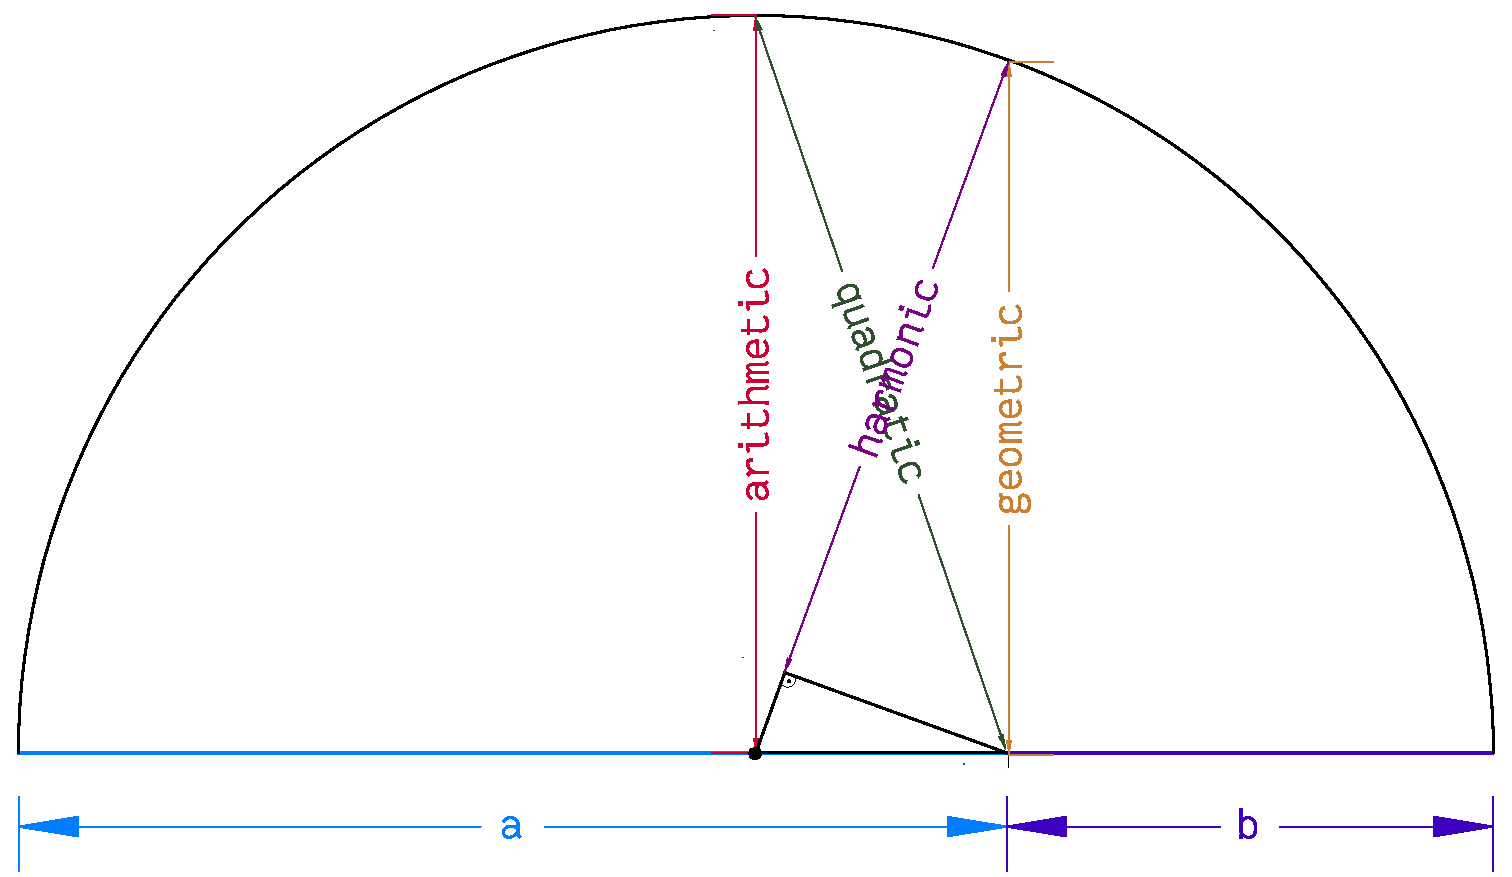
\includegraphics[width=0.75\textwidth]{Graphics/GeometricInterpretationMean}
\end{figure}

The quadratic mean (\Name{Euklid}ian mean, root mean square RMS) is defined as
\begin{equation}
  \mathrm{RMS} = \sqrt[2]{\frac{\sum_{i=1}^n{\AbsVec{x}_i^2}}{n}}
\end{equation}
The cubic mean is defined analogously. The RMS is technically important to calculate the effective voltage and current in alternating power.

The weighted \Name{Hölder}\index{Hölder@\textsc{Hölder, Ludwig Otto} 1859--1937!mean} (general) mean is defined for \( \AbsVec{x}_i \in \mathbb{R} \geq 0 \), a whole number \(z \neq 0 \) and a weight vector \AbsVec{w} with \( \sum_{i=1}^n{w_i} = 1\)
\begin{equation}
  M_\AbsVec{w}^z(\AbsVec{x}) = \sqrt[z]{\sum_{i=1}^n{\AbsVec{w}\AbsVec{x}^z_i}}
\end{equation}
where in the unweighted case all \( \AbsVec{w}_i = 1/n \). Depending on the choice of \skalar{z} we get different means:
\begin{description}
  \item[\( \lim_{z \rightarrow -\infty} \)]{minimum \( M^{-\infty}(\AbsVec{x}) = \min(\AbsVec{x}_i)  \)}
  \item[\( z = -1 \)]{harmonic mean \( M^{-1}(\AbsVec{x}) = \frac{n}{\sum_{i=1}^n{\AbsVec{x}_i^{-1}}}  \)}
  \item[\( \lim_{z \rightarrow 0} \)]{geometric mean  \( M^{0}(\AbsVec{x}) = \sqrt[n]{\prod_{i=1}^n{\AbsVec{x}_i}}  \)}
  \item[\( z = 1 \)]{arithmetic mean  \( M^1(\AbsVec{x}) = \frac{\sum_{i=1}^n{\AbsVec{x}_i}}{n}  \)}
  \item[\( z = 2 \)]{quadratic mean  \( M^2(\AbsVec{x}) = \sqrt[2]{\frac{\sum_{i=1}^n{\AbsVec{x}_i^2}}{n}}  \)}
  \item[\( z = 3 \)]{cubic mean \( M^3(\AbsVec{x}) = \sqrt[3]{\frac{\sum_{i=1}^n{\AbsVec{x}_i^3}}{n}}  \)}
  \item[\ldots]{}
  \item[\( \lim_{z \rightarrow \infty} \)]{maximum \( M^{\infty}(\AbsVec{x}) = \max(\AbsVec{x}_i)  \)}
\end{description}

\begin{lstlisting}[caption=\Name{Hölder} mean]
  FUNCTION GeneralMean(Data, Gewichte: VectorTyp; Exponent: float): float;

  VAR
    i, n: WORD;
    Sum: float;

  BEGIN
    Sum := 0;
    n := VectorLength(Data);
    IF (n = 0)
      THEN
        BEGIN
          CH := WriteErrorMessage('General mean from vector of length 0');
          DeskriptError := TRUE;
          EXIT;
        END;
    IF (n <> VectorLength(Gewichte))
      THEN
        BEGIN
          CH := WriteErrorMessage( 'General mean: unequal vector lengths of data and weights');
          DeskriptError := TRUE;
          EXIT;
        END;
    FOR i := 1 TO n DO
      Sum := Sum + GetVectorElement(Gewichte, i) * pot(GetVectorElement(Data, i), Exponent);
    Result := pot(Sum, 1 / Exponent);
  END;
\end{lstlisting}

The \textbf{f-mean} is a generalisation of the \Name{Hölder}-mean
\begin{equation}
  M_\AbsVec{w}^f = f^{-1} \left( \sum_{i=1}^n{\AbsVec{w}_i f(\AbsVec{x}_i)} \right)
\end{equation}
where in case of the \Name{Hölder}-mean \( f(\AbsVec{x}) = \AbsVec{x}^z \). For example, if \AbsVec{x} contains the returns of a capital from year 1 to \skalar{n}, then the f-mean with \( f(\AbsVec{x}) = \ln(\AbsVec{x} + 1) \) is the average return.

\subsection{Dispersion}

As discussed above, we can describe a data vector by a parameter of location, that is, a mean. However, in addition to the location, we also would like information about how much the data spread around that mean, \Foreign{i.e.}, how much error are we likely to make, if we use the mean to fill in a missing value. This is measured by parameters of dispersion.

\subsubsection{Variance and Covariance}

The covariance of two data vectors \AbsVec{X, Y} is defined as
\begin{equation}
  s_\AbsVec{x,y}^2 = 1/n \sum_{i=1}^n{(\AbsVec{x}_i - \bar{\AbsVec{x}}) (\AbsVec{y}_i - \bar{\AbsVec{y}})}
\end{equation}
The variance of a vector is the covariance with itself, \texttt{Covariance(\AbsVec{x,x})}.

To perform this calculation, two loops over the data are required, once to calculate the averages and once to calculate the variance. Here we use an alternative way that calculates both in a single loop:
\begin{align}
  s^2_1              & = 0.0  \\
  \bar{\AbsVec{x}}_1 & = \AbsVec{x}_1 \notag \\
  \bar{\AbsVec{y}}_1 & = \AbsVec{y}_1 \notag \\
  s^2_i              & = s_{i-1} \times \frac{i-2}{i-1} + \frac{(\AbsVec{x}_i - \bar{\AbsVec{x}}_{i-1})(\AbsVec{y}_i - \bar{\AbsVec{y}}_{i-1})}{i},\quad i = 2\ldots n \notag \\
  \bar{\AbsVec{x}}_i & = \bar{\AbsVec{x}}_{i-1} + \frac{\AbsVec{x}_i - \bar{\AbsVec{x}}_{i-1}}{i} \notag \\
  \bar{\AbsVec{y}}_i & = \bar{\AbsVec{y}}_{i-1} + \frac{\AbsVec{y}_i - \bar{\AbsVec{y}}_{i-1}}{i} \notag
\end{align}

\begin{lstlisting}[caption=Covariance of two vectors]
  FUNCTION Covariance(CONST X, Y: VectorTyp): float;

  VAR
    n, Count, i, j: WORD;
    CH: CHAR;
    xi, yi, xAv, yAv, s: float;

  BEGIN
    n := VectorLength(X);
    IF (n = 0)
      THEN
        BEGIN
          CH := WriteErrorMessage('Covariance from vector of length 0');
          DeskriptError := TRUE;
          EXIT;
        END;
    IF (n <> VectorLength(Y))
      THEN
        BEGIN
          CH := WriteErrorMessage('Covariance of vectors of unequal length ');
          DeskriptError := TRUE;
          EXIT;
        END;
    j := 0;
    REPEAT                            // find first complete pair OF data
      INC(j);
      xi := GetVectorElement(X, j);
      yi := GetVectorElement(Y, j);
    UNTIL NOT (IsNaN(xi) OR IsNaN(yi));
    xAv := xi;
    yAv := yi;
    s := 0.0;
    Count := 1;
    FOR i := Succ(j) TO n DO
      BEGIN
        xi := GetVectorElement(X, i);
        yi := GetVectorElement(Y, i);
        IF (IsNan(xi) OR IsNaN(yi))
          THEN
          ELSE
            BEGIN
              INC(Count);
              s := s * ((Count - 2) / (Count - 1)) + (xi - xAv) * (yi - yAv) / Count;
              xAv := xAv + (xi - xAv) / Count;
              yAv := yAv + (yi - yAv) / Count;
            END;
      END;
    Result := s;
  END;


  FUNCTION Variance(Data: VectorTyp): float;

  BEGIN
    Result := Covariance(Data, Data);
  END;
\end{lstlisting}

The standard deviation \skalar{\sigma} of a data vector is the square root of its variance. It has the same unit as the mean, which makes them comparable. If the data are normally distributed,   \SI{68.3}{\%} of the data will be within the range \( \pm \sigma \), \SI{95.4}{\%} within \( \pm 2\sigma \) and \SI{99.7}{\%} within \( \pm 3\sigma \).
\begin{lstlisting}
   function StandardDeviation(var Data: VectorTyp): float;

   begin
     Result := sqrt(Covariance(Data, Data));
   end;
\end{lstlisting}

The standard error of the mean is \( \sigma_{\bar{\AbsVec{x}}} =  \frac{\sqrt{\sigma^2}}{\sqrt{n}} \), thus, increasing \skalar{n} will decrease this error, but with diminishing return.
\begin{lstlisting}
  FUNCTION StandardErrorOfMean(v: float; n: WORD): float;

  BEGIN
    IF n > 0
      THEN
        StandardErrorOfMean := Sqrt(v) / Sqrt(n)
      ELSE
        BEGIN
          WriteErrorMessage(' Standard error of mean for n = 0');
          DeskriptError := TRUE;
        END;
  END;
\end{lstlisting}



The coefficient of variation (unitised risk) is the standard deviation divided by the absolute value of the mean: \( \mathrm{CV} = \frac{\sqrt{\sigma^2}}{|\mu|} \), often multiplied with \SI{100}{\%}. It is used to express the precision of an assay. As a number without unit it is independent of the unit in which the data were measured. Warning: If the data are not measured on a rational scale, the mean may be zero (\Foreign{e.g.}, temperatures on the \si{\celsius} scale near freezing) and the CV is affected by small fluctuations of the mean.
\begin{lstlisting}
  FUNCTION CoefficientOfVariation(Mean, v: float; n: WORD): float;

  BEGIN
    IF Abs(mean) > Zero
      THEN
        Result := Sqrt(v) / Abs(Mean)
      ELSE
        BEGIN
          WriteErrorMessage(' Coefficient of variation with mean 0');
          DeskriptError := TRUE;
        end;
  END;
\end{lstlisting}

\subsubsection{Other measures of dispersion}

Alternatively, on can calculate the distance of all data points from the mean, and then determine the mean or median of those:
\begin{lstlisting}
  FUNCTION MeanDeviationFromMean(Data: VectorTyp): float;

  VAR
    Mean, Sum: float;
    i, j, n: WORD;

  BEGIN
    n := VectorLength(Data);
    IF (n = 0)
      THEN
        BEGIN
          CH := WriteErrorMessage('Mean deviation of mean from vector of length 0');
          DeskriptError := TRUE;
          EXIT;
        END;
    Mean := ArithmeticMean(Data);
    Sum := 0;
    FOR i := 1 TO n DO
      Sum := Sum + Abs(Mean - GetVectorElement(Data, i));
    Result := Sum / n;
  END;


  FUNCTION MedianDeviationFromMean(Data: VectorTyp): float;

  VAR
    Mean: float;
    Abweichungen: VectorTyp;
    i: WORD;

  BEGIN
    CreateVector(Abweichungen, VectorLength(Data), 0.0);
    Mean := ArithmeticMean(Data);
    CreateVector(Abweichungen, VectorLength(Data), 0.0);
    FOR i := 1 TO VectorLength(Data) DO
      SetVectorElement(Abweichungen, i, Abs(Mean - GetVectorElement(Data, i)));
    ShellSort(Abweichungen);
    MedianDeviationFromMean := Median(Abweichungen);
    DestroyVector(Abweichungen);
  END;
\end{lstlisting}

\subsection{\Name{Pearson} moments}

Moments describe the shape of a distribution curve. The 0th moment is the total probability, that is, the integral of the distribution curve and hence always unity. The 1st moment is the expected value, that is, the mean. The 2nd moment is the variance. The 3rd moment is the skewness (lopsidedness, asymmetry), the 4th moment the kurtosis (heaviness of the tail). Higher moments can be defined, but are not commonly used. The moment is calculated from
\begin{equation}
  \mu_k = \frac{1}{n} \sum_{i=1}^n{(\AbsVec{x}_i-\bar{\AbsVec{x}})^k}
\end{equation}
They are then standardised by dividing them by \skalar{\sigma^k}.

\begin{lstlisting}
  FUNCTION Mue(CONST Data: VectorTyp; Mean: float; k: WORD): float;

  VAR
    Sum: float;
    i, n: WORD;

  BEGIN
    Sum := 0;
    n := VectorLength(Data);
    IF (n = 0)
      THEN
        BEGIN
          CH := WriteErrorMessage('Mue from vector of length 0');
          DeskriptError := TRUE;
          EXIT;
        END;
    FOR i := 1 TO n DO
      Sum := Sum + pot(GetVectorElement(Data, i) - Mean, k);
    Result := Sum / n;
  END;
\end{lstlisting}

Skewness, \( \mu_3/\sigma^3\), is a measure of asymmetry of a distribution, and can be
\begin{description}
  \item[negative]{tail is on the left side, left-skewed = right-leaning}
  \item[zero]{the tails balance, but the distribution is not necessarily symmetrical}
  \item[positive]{tail is on the right side, right-skewed = left-leaning}
\end{description}
, at least for simple unimodal distributions.

\begin{lstlisting}
  FUNCTION Skewness(CONST Data: VectorTyp; Mean, StaDev: float): float;

  BEGIN
    Result := Mue(Data, Mean, 3) / pot(StaDev, 3);
  END;
\end{lstlisting}

Alternative measures of skewness have been suggested by \Name{Pearson}:
\begin{equation}
  \frac{\bar{\AbsVec{x}} - \mathrm{mode}(\AbsVec{x})}{\sigma},\ \frac{3 \bar{\AbsVec{x}} - \breve{\AbsVec{x}}}{\sigma}
\end{equation}

The kurtosis (from Gr. curved, arching) is the 4th standardised \Name{Pearson} moment \( \mu_4/\sigma^4\). Data within one standard deviation of the mean contribute little to its value, because raising the \skalar{z}-standardised datum to the 4th power will make them close to zero. Only data away from the peak -- that is, outliers -- contribute to the kurtosis. The kurtosis parameter is a measure of the combined weight of the tails, relative to the centre of the distribution. The normal distribution has a kurtosis of \num{3}. Thus, we get the \textbf{excess kurtosis} by subtracting \num{3} from the moment. The result can be
\begin{description}
  \item[negative]{, then the distribution is called platykurtic and has fewer and less extreme outliers }
  \item[zero]{, then the distribution is called mesokurtic and has about as many outliers}
  \item[positive]{, then the distribution is called leptokurtic and has more, and more extreme outliers}
\end{description}
than the normal distribution.

\begin{lstlisting}
  FUNCTION ExcessKurtosis(CONST Data: VectorTyp; Mean, StaDev: float): float;

  BEGIN
    Result := (Mue(Data, Mean, 4) / pot(StaDev, 4)) - 3.0;
  END;
\end{lstlisting}

\subsection{Concentration}

\subsubsection{\Name{Lorenz-Münzner}-curve and \Name{Gini}-coefficient}

\begin{figure}
 \caption{\Name{Lorenz-Münzner}-plot. For details see text. }
 \label{fig:Lorenz}
 \centering
 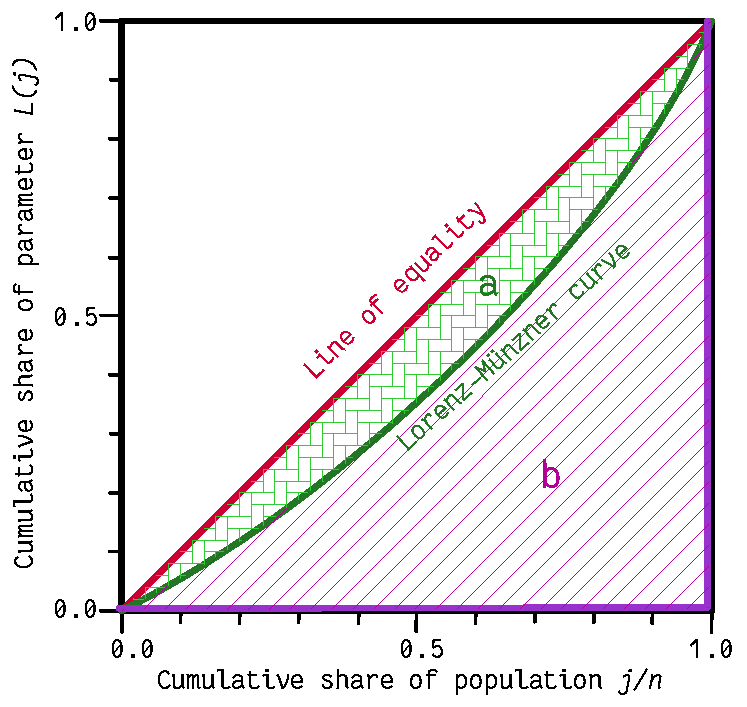
\includegraphics[width=0.75\textwidth]{Graphics/Lorenz-Munzner}
\end{figure}

The \Name{Lorenz-Münzner} curve of an data vector \AbsVec{x} sorted in non-decreasing order (see fig. \ref{fig:Lorenz}) is given by
\begin{equation}
  L(j) = \sum_{i=1}^j{\frac{\AbsVec{x}_i}{n\mu}} = \sum_{i=1}^j{\AbsVec{l}_j}
\end{equation}
and is the cumulative fraction of the data for every position \skalar{j}. If \( \AbsVec{x}_i = \mu\ \forall\ i \) (all data are the same), then a plot of \skalar{L(j)} vs \skalar{j/n} is a straight line through the origin with slope  one (line of equality, \emph{red}). In the other extreme, if all \skalar{\AbsVec{x}_i} except one are zero, then the \Name{Lorenz-Münzner} curve consist of two straight lines (\emph{purple}), one from (0, 0) to (1, 0) and the second perpendicular to (1, 1) . Together with the line of equality, they form a triangle with area \num{0.5}.

Real data will form a curve between those extremes, and the \Name{Gini}-coefficient \parencite{Gin-36} is the area between this curve and the line of equality, divided by the area of the triangle: \( G = a/(a + b) \), because \( a + b = 0.5 \), this is equal to \( G = 2a \). If \( \AbsVec{x}_i \geq 0\ \forall\ i \), the \Name{Gini}-coefficient ranges from \( 0\ldots 1 \). If the parameter is distributed equally, and all data are on the line of equality, the \Name{Gini}-coefficient is zero, in case of maximal inequality it becomes \num{1}. Thus
\begin{equation}
   G = 2 a = \sum_{i=1}^n{\AbsVec{l}_i \left( \frac{i-1}{n} + \frac{i}{n} \right)} - \frac{1}{2} = \sum_{i=1}^n{\AbsVec{l}_i \frac{2i - n - 1}{2n}}
\end{equation}

\begin{lstlisting}
  FUNCTION LorenzMuenzner(Data: VectorTyp; VAR xVektor, yVektor: VectorTyp): float;

  VAR
    n, i: WORD;
    u, v, Sum, Gesamt, SumV: float;

  BEGIN
    n := VectorLength(Data);
    IF (n = 0)
      THEN
        BEGIN
          CH := WriteErrorMessage('Lorenz-Muenzner from vector of length 0');
          DeskriptError := TRUE;
          EXIT;
        END;
    CreateVector(xVektor, n, 0.0);
    CreateVector(yVektor, n, 0.0);
    Gesamt := NeumaierSum(Data);
    v := 0;
    Sum := 0;
    SumV := 0;
    FOR i := 1 TO n DO
      BEGIN
        u := i / n;
        Sum := Sum + GetVectorElement(Data, i);
        v := Sum / Gesamt;
        SetVectorElement(xVektor, i, u);
        SetVectorElement(yVektor, i, v);
        SumV := SumV + v;
      END;
    Result := (Succ(n) - 2 * SumV) / (Pred(n));
  END;
\end{lstlisting}

Alternatively, one can define the \Name{Gini}-Coefficient as half the sum of the absolute difference of all pairs of items \( |\AbsVec{x}_i - \AbsVec{x}_j| \) normalised by the average \skalar{\bar{\AbsVec{x}}}. This does not require sorting of the data vector:
\begin{equation}
  G = \frac{\sum_{i=1}^n{\sum_{j=1}^n{|\AbsVec{x}_i - \AbsVec{x}_j|}}}{2\sum_{i=1}^n{\AbsVec{x}_j}} = \frac{\sum_{i=1}^n{\sum_{j=1}^n{|\AbsVec{x}_i - \AbsVec{x}_j|}}}{2 n^2 \bar{\AbsVec{x}}}
\end{equation}

\begin{lstlisting}
  FUNCTION Gini(Data: VectorTyp; Mean: float): float;
    { mittlere Abweichung aller Data voneinander }

  VAR
    i, j, n: WORD;
    Sum: float;

  BEGIN
    Sum := 0;
    n := VectorLength(Data);
    IF (n = 0)
      THEN
        BEGIN
          CH := WriteErrorMessage('Gini coefficient from vector of length 0');
          DeskriptError := TRUE;
          EXIT;
        END;
    FOR i := 1 TO Pred(n) DO
      FOR j := Succ(i) TO n DO
        Sum := Sum + Abs(GetVectorElement(Data, i) - GetVectorElement(Data, j));
    Result := Sum / (2 * n * n * Mean);
  END;
\end{lstlisting}

\subsubsection{The \Name{Herfindahl-Hirschman}-Index}

This measure of concentration is often used by anti-trust authorities to calculate the concentration of producers in a market. It is defined as
\begin{equation}
  H = \sum_{i=1}^n{\left( \frac{\AbsVec{x}_i}{\sum_{j=1}^n{\AbsVec{x}_j}} \right)^2}
\end{equation}
, that is, the sum of the squared relative market shares, and reaches from \skalar{1/n} to 1. \skalar{1/H} is the effective number of competitors in the market. The index is equivalent to the \textbf{\Name{Simpson} diversity index} in ecology or the \textbf{effective number of parties index} in politics. The squaring gives additional weight to the larger companies. In economy, we consider markets with \( H < \)
\begin{description}
  \item[0.01]{highly competitive}
  \item[0.15]{unconcentrated}
  \item[0.25]{moderately concentrated}
  \item[beyond]{highly concentrated}
\end{description}
One can normalise H to the range 0\ldots 1 by \( H^* = \frac{H - 1/n}{1 - 1/n} \).

\begin{lstlisting}
  FUNCTION HerfindahlIndex(Data: VectorTyp): float;

  VAR
    n, i: WORD;
    Sum1, Sum2: float;

  BEGIN
    n := VectorLength(Data);
    IF (n = 0)
      THEN
        BEGIN
          CH := WriteErrorMessage('Herfindahl index from vector of length 0');
          DeskriptError := TRUE;
          EXIT;
        END;
    Sum1 := NeumaierSum(Data);
    Sum2 := 0;
    FOR i := 1 TO n DO
      Sum2 := Sum2 + Sqr(GetVectorElement(Data, i) / Sum1);
    Result := Sum2;
  END;
\end{lstlisting}


\section{Non-parametric measures}

\subsubsection{Location}

\paragraph{Median and related measures}

The \texttt{LowMed} of a sorted data vector is the low median (the \( [(n+1)\ \mathrm{div}\ 2] \)-th smallest element \( \AbsVec{x}_{\left((n+1)\ \mathrm{div}\ 2\right)} \)) and \texttt{HiMed} the high median (the \( [(n\ \mathrm{div}\ 2) + 1] \)-th smallest element \( \AbsVec{x}_{\left((n\ \mathrm{div}\ 2) + 1\right)} \) ). For odd \skalar{n}, low and high median are identical, for even \skalar{n} they are different. The common median \( \breve{\AbsVec{x}} \) is the average between \texttt{LoMed} and \texttt{HiMed}. It is equivalent to the 2nd quartile \(Q_2 \) of the data. The \skalar{k}-th smallest element of a vector \AbsVec{x} is called its \skalar{k}-th order statistics, \( \AbsVec{x}_{(k)} \).

\begin{lstlisting}[caption=Median of a data vector]
  FUNCTION HiMed(CONST SortedData: VectorTyp): float;

  VAR
    n: WORD;

  BEGIN
    n := VectorLength(SortedData);
    IF (n = 0)
      THEN
        BEGIN
          CH := WriteErrorMessage('Hi median from vector of length 0');
          DeskriptError := TRUE;
        END
    ELSE
      Result := GetVectorElement(SortedData, Succ(n DIV 2));
  END;

  FUNCTION LoMed(CONST SortedData: VectorTyp): float;

  VAR
    n: WORD;

  BEGIN
    n := VectorLength(SortedData);
    IF (n = 0)
      THEN
        BEGIN
          CH := WriteErrorMessage('Low median from vector of length 0');
          DeskriptError := TRUE;
        END
      ELSE
        Result := GetVectorElement(SortedData, Succ(n) DIV 2);
  END;

  FUNCTION Median(VAR Data: VectorTyp): float;

  VAR
    n: WORD;
    Sorted: VectorTyp;

  BEGIN
    n := VectorLength(Data);
    IF (n = 0)
      THEN
        BEGIN
          CH := WriteErrorMessage('Median from vector of length 0');
          DeskriptError := TRUE;
          EXIT;
        END;
    ShellSort(Data);
    IF Odd(n)
      THEN Median := LoMed(Data)  // LOW AND Hi median are identical
      ELSE Median := (LoMed(Data) + HiMed(Data)) / 2;
  END;
\end{lstlisting}

The median is a special case of a quantile, namely \SI{50}{\%}, also called \skalar{Q_2} for second quartile. Other important quantiles are \skalar{Q_1} and \skalar{Q_3}, which correspond to the \SI{25}{\%} and \SI{75}{\%} quantiles, respectively. However, for the calculations of quantiles, we do not calculate the average between neighbouring elements. Rather, we take the higher of the two elements.

\begin{lstlisting}[caption=Quantiles of a data vector]
  FUNCTION Quantile(VAR Data: VectorTyp; q: float): float;

  VAR
    n: WORD;

  BEGIN
    n := VectorLength(Data);
    IF (n = 0)
      THEN
        BEGIN
          CH := WriteErrorMessage('Quantile from vector of length 0');
          DeskriptError := TRUE;
          EXIT;
        END;
    ShellSort(Data);
    Result := GetVectorElement(Data, Round(n * q + 0.5)); // always Round up
  END;
\end{lstlisting}

The trimedian is a measure of location that is particularly robust against outliers. It is defined as \(  \frac{Q_1 + 2 Q_2 + Q_3}{4} \).

\begin{lstlisting}
  FUNCTION TriMedian(Data: VectorTyp): float;

  VAR
    n: WORD;

  BEGIN
    n := VectorLength(Data);
    IF (n = 0) THEN
    BEGIN
      CH := WriteErrorMessage('Trimedian from vector of length 0');
      DeskriptError := TRUE;
      EXIT;
    END;
    Result := (Quantile(Data, 0.25) + 2 * Quantile(Data, 0.5) +
      Quantile(Data, 0.75)) / 4;
  END;
\end{lstlisting}

If the individual data have different reliabilities, then it is possible to assign weights to them so that \( \sum_{i=1}^n{w_i} = 1 \). Then, for data sorted in ascending order of \AbsVec{x},  the \texttt{LoMed} is the last element for which \( \sum_{i=1}^n{\AbsVec{w}_i} \leq 0.5 \), and the \texttt{HiMed} the first element for which this sum is \( \geq 0.5 \). Again, the median is the average of the two. Here, we assume that the data are in the first, and the weights in the second column of a matrix.

\begin{lstlisting}
  FUNCTION WeightedHiMed(CONST SortedData: MatrixTyp): float;

  VAR
    i: WORD;
    Sum: float;

  BEGIN
    Sum := 0.0;
    i := 0;
    REPEAT
      INC(i);
      sum := sum + GetMatrixElement(SortedData, i, 2);
    UNTIL (sum >= 0.5);
    WeightedHiMed := GetMatrixElement(SortedData, i, 1);
  END;

  FUNCTION WeightedLoMed(CONST SortedData: MatrixTyp): float;

  VAR
    i: WORD;
    Sum: float;

  BEGIN
    Sum := 0.0;
    i := 0;
    REPEAT
      INC(i);
      sum := sum + GetMatrixElement(SortedData, i, 2);
      IF (sum > 0.5) THEN DEC(i);
    UNTIL (sum >= 0.5);
    WeightedLoMed := GetMatrixElement(SortedData, i, 1);
  END;

  FUNCTION WeightedMedian(VAR Data: MatrixTyp): float;

  VAR
    n: WORD;

  BEGIN
    n := MatrixRows(Data);
    IF (n = 0)
      THEN
        BEGIN
          CH := WriteErrorMessage('Weighted median from vector of length 0');
          DeskriptError := TRUE;
          EXIT;
        END;
    ShellSortMatrix(Data, 1);
    WeightedMedian := (WeightedLoMed(Data) + WeightedHiMed(Data)) / 2.0;
  END;
\end{lstlisting}

\paragraph{Other measures of location}

The median has a discontinuous influence function. Instead, one can use the \Name{Hodges-Lehmann}-estimator \parencite{Hod-63}, which is the median of \( \frac{\AbsVec{x}_i + \AbsVec{x}_j}{2}, i < j \), that is, the median over all \( \binom{n}{2} \) pairwise averages of the data vector. The naive implementation would be

\begin{lstlisting}
  FUNCTION NaiveHodgesLehmann(Data: VectorTyp): float;

  VAR
    n, i, j, k: WORD;
    x, y: float;
    Averages: VectorTyp;

  BEGIN
    n := VectorLength(Data);
    IF (n = 0)
      THEN
        BEGIN
          CH := WriteErrorMessage('Hodges-Lehmann estimator from vector of length 0');
          DeskriptError := TRUE;
          EXIT;
        END;
    n := Round(BinomialCoef(n, 2));
    CreateVector(Averages, n, 0.0);
    k := 0;
    FOR i := 1 TO VectorLength(Data) DO
      BEGIN
        x := GetVectorElement(Data, i);
        FOR j := 1 TO Pred(i) DO
          BEGIN
            INC(k);
            y := GetVectorElement(Data, j);
            SetVectorElement(Averages, k, (x + y) / 2);
          END;
      END;
    Result := Median(Averages);
    DestroyVector(Averages);
  END;
\end{lstlisting}

The problem with this implementation is, that \( \binom{n}{2} \leq \mathrm{MaxVector} = \num{10000} \) is fulfilled only for \( n \leq \num{141} \) . %Actually, 362 still works, but 363 fails
To find a more memory-efficient implementation, we first consider that all averages must be from the range \( \max(\AbsVec{x}) - \min(\AbsVec{x}) \). If we divide this range into a moderate number \texttt{NrBins} of subranges of equal size we can count the frequencies of averages in those subranges. The bin number \texttt{bins} is thus
\begin{equation}
  \mathrm{Bin}(\mathrm{Average}) = \frac{\mathrm{Average} - \min(\AbsVec{x})}{\mathrm{Step}},\ \mathrm{Step} = \frac{\max(\AbsVec{x}) - \min(\AbsVec{x})}{\mathrm{NrBins}}
\end{equation}
To get to the median, we simply add the frequencies starting from subrange 0 until the sum reaches \( \binom{n}{2} / 2 \). There is some quantisation error, but if the bin size is chosen small enough, this shouldn't matter. What does ``small enough'' mean? For data classification, the number of classes is commonly chosen as \( \sqrt{n} \), so that the information loss and clarity are balanced and, in addition, most classes are occupied. Thus, the optimal number of classes would be \( \sqrt{\binom{n}{2}} \), a maximum of \num{10000} bins would then be sufficient for a data vector of length \num{14142}. The relative difference between the results of both implementations with synthetic data is in the order \num{e-3}.

\begin{lstlisting}
  FUNCTION HodgesLehmann(Data: VectorTyp): float;

  VAR
    min, max, Step, Sum, x, y: float;
    Counts: VectorTyp;
    i, j, n, NrBins, Bin: WORD;

  BEGIN
    n := VectorLength(Data);
    IF (n = 0)
      THEN
        BEGIN
          CH := WriteErrorMessage('Hodges-Lehmann estimator from vector of length 0');
          DeskriptError := TRUE;
          EXIT;
        END;
    NrBins := Round(Sqrt(BinomialCoef(n, 2)));
    min := FindSmallest(Data);
    max := FindLargest(Data);
    IF (min = max)
      THEN
        BEGIN
          CH := WriteErrorMessage('Hodges-Lehmann estimator: all data are the same');
          DeskriptError := TRUE;
          EXIT;
        END;
    Step := (max - min) / NrBins;
    CreateVector(Counts, Succ(NrBins), 0.0);  // because vector starts at 1, rather than 0
    FOR i := 1 TO n DO                        // count frequency OF grouped averages
      BEGIN
        x := GetVectorElement(Data, i);
        FOR j := 1 TO Pred(i) DO
          BEGIN
            y := GetVectorElement(Data, j);
            Bin := Succ(Round(((x + y) / 2 - min) / Step));
            SetVectorElement(Counts, Bin, GetVectorElement(Counts, Bin) + 1.0);
          END;
      END;
    Sum := 0.0;
    i := 0;
    REPEAT                                    // identify bin OF median
      INC(i);
      Sum := Sum + GetVectorElement(Counts, i);
    UNTIL sum >= (BinomialCoef(n, 2) / 2);
    HodgesLehmann := Pred(i) * Step + min;
    DestroyVector(Counts);
  END;
\end{lstlisting}

\subsubsection{Dispersion}

The interquartile distance (\( 0.5 (Q_3 - Q_1) \)) can be used as probable range of \AbsVec{x} in the same sense as standard deviation. Although simple to calculate, the breakdown point of the interquartile distance is \SI{25}{\%}.

\begin{lstlisting}
  FUNCTION InterQuantilDistance(Q1, Q3: float): float;

  BEGIN
    Result := 0.5 * (Q3 - Q1);
  END;
\end{lstlisting}

\begin{lstlisting}
  FUNCTION QuantileDispersionCoefficient(Q1, Q3: float): float;

  BEGIN
    QuantileDispersionCoefficient := (Q3 - Q1) / (Q3 + Q1);
  END;
\end{lstlisting}

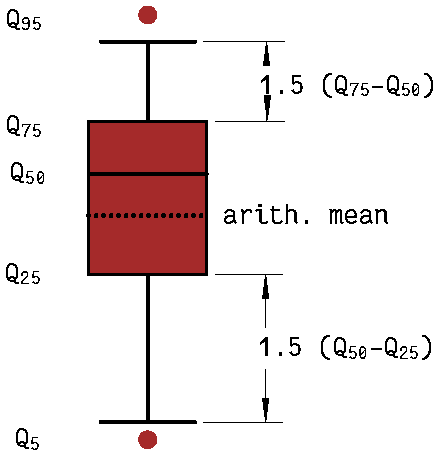
\includegraphics[width=0.25\textwidth]{Graphics/Box-and-Wisker} The quartiles are used also to create \textbf{box-and-whisker plots}, where the box encompasses the interquartile range and the whiskers have the length of \(1.5 (Q_{50}-Q_{25} \) and \(1.5 (Q_{75}-Q_{50}) \), respectively. Data outside the whisker range are considered outliers. They can be placed individually, or the \skalar{Q_5} and \skalar{Q_{95}}-points are marked instead. Marking the arithmetic mean by a dotted line is optional, but gives a good idea about the skew of the data. This plot is very good for comparing data vectors obtained under different experimental conditions for position and spread.

The coefficient of quartile deviation \( \frac{Q3-Q1}{Q3+Q1} \) is another measure of dispersione.

\begin{lstlisting}
  FUNCTION StandardErrorOfMedian(Data: VectorTyp): float;

  VAR
    i, j, n: WORD;

  BEGIN
    n := VectorLength(Data);
    IF (n = 0)
      THEN
        BEGIN
          CH := WriteErrorMessage('Weighted low median from vector of length 0');
          DeskriptError := TRUE;
          EXIT;
        END;
    i := Round(n / 2 - Sqrt(3 * n) / 2);
    j := Round(n / 2 + Sqrt(3 * n) / 2);
    Result := (GetVectorElement(Data, j) - GetVectorElement(Data, i)) / 3.4641;
  END;
\end{lstlisting}

The \acf{MAD} \parencite{Rou-93} is the median of \( |\AbsVec{x}_i - \breve{\AbsVec{x}}| \), a robust measure of dispersion with a breakdown point of \SI{50}{\%} of the data. It is thus more useful than the interquartile distance. To make the \acs{MAD} consistent with other measures of dispersion, it needs to be multiplied by a scaling parameter, to make it consistent with the standard deviation \skalar{\sigma}, this parameter is \( \frac{1}{\sqrt{2}} \mathrm{qnorm}\left(\frac{5}{8}\right) = \num{1.4826} \). To detect outliers in the data vector, one can flag those \( \AbsVec{x}_i \), whose \( \frac{|\AbsVec{x}_i - \breve{\AbsVec{x}}|}{\mathrm{MAD}(\AbsVec{x})} \) exceeds a cutoff, for example \num{2.5} or \num{3.0}. However, this assumes a distribution symmetrical around the median.

\begin{lstlisting}[caption=median absolute deviation from median (MAD)]
  FUNCTION MAD(Data: VectorTyp): double;

  CONST
    Scale = 1.4826; //   1 / (Sqrt(2) * qnorm(5/8))

  VAR
    m, Sum, cn: float;
    n, i: WORD;
    Dev: VectorTyp;

  BEGIN
    n := VectorLength(Data);
    IF (n = 0)
      THEN
        BEGIN
          CH := WriteErrorMessage('MAD from vector of length 0');
          DeskriptError := TRUE;
          EXIT;
        END;
    m := Median(Data);
    CreateVector(Dev, n, 0.0);
    FOR i := 1 TO n DO
      SetVectorElement(Dev, i, Abs(GetVectorElement(Data, i) - m));
    CASE n OF
      2: cn := 1.196;
      3: cn := 1.495;
      4: cn := 1.363;
      5: cn := 1.206;
      6: cn := 1.200;
      7: cn := 1.140;
      8: cn := 1.129;
      9: cn := 1.107
      ELSE
        cn := n / (n - 0.8);
    END; { case }
    MAD := cn * Scale * Median(Dev);
    DestroyVector(Dev);
  END;
\end{lstlisting}

To calculate \acs{MAD} as parameter of dispersion, one first has to calculate \skalar{\breve{\AbsVec{x}}} as parameter of position.

Dispersion parameters corresponding to the \Name{Hodges-Lehmann}-estimator of location are \skalar{S_n} and \skalar{Q_n} \parencite{Rou-93}:
\begin{eqnarray}
  S_n &=& c_n \times 1.1926 \times \mathrm{lomed}_{i = 1\ldots n}\left(\mathrm{himed}_{j \neq i} |\AbsVec{x}_i - \AbsVec{x}_j|\right)\\
  Q_n &=& c_n \times 2.2219 \times [|\AbsVec{x}_i - \AbsVec{x}_j|, i < j]_{(k)}
\end{eqnarray}
The constant factor is for consistency at normal distribution, \skalar{c_n} is a finite sample correction factor. For a maximal breakdown point, \( k = \binom{n}{s}/4 \). For both \skalar{S_n} and \skalar{Q_n}, the breakdown point is \( (n\ \mathrm{div}\ 2)\ \mathrm{div}\ n \), the best possible value \parencite{Cro-92}. \Name{Gauss}ian asymptotic efficiency is \SI{58}{\%} for \skalar{S_n}, and even \SI{82}{\%} for \skalar{Q_n}. If we divide \skalar{Q_n} by \( \sqrt{n} \), we get a robust standard error.

\begin{lstlisting}[caption= naive Sn and Qn: \textbf{O}($n^2$)]
  FUNCTION NaiveSn(VAR Data: VectorTyp): float;

  VAR
    i, j, n: WORD;
    a1, a2: VectorTyp;
    xi, cn: float;

  BEGIN
    n := VectorLength(Data);
    IF (n = 0)
      THEN
        BEGIN
          CH := WriteErrorMessage('Sn from vector of length 0');
          DeskriptError := TRUE;
          EXIT;
        END;
    CreateVector(a1, n, 0.0);
    CreateVector(a2, n, 0.0);
    FOR i := 1 TO n DO
      BEGIN
        xi := GetVectorElement(Data, i);
        FOR j := 1 TO n DO
          SetVectorElement(a1, j, Abs(xi - GetVectorElement(Data, j)));
        ShellSort(a1);
        SetVectorElement(a2, i, GetVectorElement(a1, Succ(n DIV 2))); // high median
      END;
    DestroyVector(a1);
    ShellSort(a2);
    CASE n OF
      2: cn := 0.743;
      3: cn := 1.851;
      4: cn := 0.954;
      5: cn := 1.351;
      6: cn := 0.993;
      7: cn := 1.198;
      8: cn := 1.005;
      9: cn := 1.131
      ELSE IF Odd(n)
             THEN cn := n / (n - 0.9)
             ELSE cn := 1;
    END; { case }
    Result := cn * 1.1926 * GetVectorElement(a2, Succ(n) DIV 2);  // LOW median
  END;



  FUNCTION NaiveQn(VAR Data: VectorTyp): float;

  VAR
    i, j, n, k: WORD;
    a1: VectorTyp;
    xi, dn: float;

  BEGIN
    n := VectorLength(Data);
    IF (n = 0)
      THEN
        BEGIN
          CH := WriteErrorMessage('Qn from vector of length 0');
          DeskriptError := TRUE;
          EXIT;
        END;
    CreateVector(a1, (n - 1) * n DIV 2, 0.0);
    k := 0;
    FOR i := 1 TO n DO
      BEGIN
        xi := GetVectorElement(Data, i);
        FOR j := Succ(i) TO n DO
          BEGIN
            INC(k);
            SetVectorElement(a1, k, Abs(xi - GetVectorElement(Data, j)));
          END;
      END;
    ShellSort(a1);
    CASE n OF   // finite sample correction factor
      2: dn := 0.399;
      3: dn := 0.994;
      4: dn := 0.512;
      5: dn := 0.844;
      6: dn := 0.611;
      7: dn := 0.857;
      8: dn := 0.669;
      9: dn := 0.872;
      ELSE
        IF Odd(n)    // n >= 10
          THEN dn := n / (n + 1.4)
          ELSE dn := n / (n + 3.8);
    END; { case }
    xi := GetVectorElement(a1, Round(BinomialCoef(n, 2)) DIV 4);
    Result := dn * 2.2219 * xi;
    DestroyVector(a1);
  END;
\end{lstlisting}

These algorithms are \textbf{O}(\skalar{n^2}), and the naive Qn implementation is limited to \skalar{n} = 141 by available memory. However, they can be made \textbf{O}(\skalar{n} log(\skalar{n})) with \textbf{O}(\skalar{n}) storage space requirement \parencite{Cro-92}.

\begin{lstlisting}[caption= final Sn: \textbf{O}($n \log(n)$)]
  FUNCTION Sn(VAR Data: VectorTyp): float;

  VAR
    n, i, j, l, nA, nB, rightA, rightB, leftA, leftB, tryA, tryB, diff,
    Amin, Amax, even, half: WORD;
    cn, medA, medB: float;
    a2: VectorTyp;

  BEGIN
    n := VectorLength(Data);
    IF (n = 0)
      THEN
        BEGIN
          CH := WriteErrorMessage('Sn from vector of length 0');
          DeskriptError := TRUE;
          EXIT;
        END;
    ShellSort(Data);
    CreateVector(a2, n, 0.0);
    SetVectorElement(a2, 1, GetVectorElement(Data, Succ(n DIV 2)) -
      GetVectorElement(Data, 1));
    FOR i := 2 TO (Succ(n) DIV 2) DO // a2(i) = lomed_{j<>i} | xi - xj |, i = 2...Succ(n)/2
      BEGIN
        nA := Pred(i);
        nB := n - i;
        diff := nB - nA;
        leftA := 1;
        leftB := 1;
        rightA := nB;
        rightB := nB;
        Amin := Succ(diff DIV 2);
        Amax := diff DIV 2 + nA;
        WHILE (leftA < rightA) DO
          BEGIN
            l := Succ(rightA - leftA);
            even := 1 - (l MOD 2);
            half := Pred(l) DIV 2;
            tryA := leftA + half;
            tryB := leftB + half;
            IF (tryA < Amin)
              THEN
                BEGIN
                  rightB := tryB;
                  leftA := tryA + even;
                END
              ELSE IF (tryA > Amax)
                     THEN
                       BEGIN
                         rightA := tryA;
                         leftB := tryB + even;
                       END
                     ELSE
                       BEGIN
                         medA := GetVectorElement(Data, i) - GetVectorElement(Data, (i - tryA + Amin - 1));
                         medB := GetVectorElement(Data, tryB + i) - GetVectorElement(Data, i);
                         IF (medA >= medB)
                           THEN
                             BEGIN
                               rightA := tryA;
                               leftB := tryB + even;
                             END
                           ELSE
                             BEGIN
                               rightB := tryB;
                               leftA := tryA + even;
                             END;
                       END;
          END; { while }
        IF (leftA > Amax)
          THEN
            SetVectorElement(a2, i, GetVectorElement(Data, leftB + i) -
                             GetVectorElement(Data, i))
          ELSE
            BEGIN
              medA := GetVectorElement(Data, i) - GetVectorElement(Data,
                Pred(i - leftA + Amin));
              medB := GetVectorElement(Data, leftB + i) - GetVectorElement(Data, i);
              SetVectorElement(a2, i, min(medA, medB));
            END;
      END; { for }
    FOR i := Succ(Succ(n) DIV 2) TO Pred(n) DO    // same, but i = Succ(Succ(n)/2) ... n-1
      BEGIN
        nA := n - i;
        nB := Pred(i);
        diff := nB - nA;
        leftA := 1;
        leftB := 1;
        rightA := nB;
        rightB := nB;
        Amin := Succ(diff DIV 2);
        Amax := diff DIV 2 + nA;
        WHILE (leftA < rightA) DO
          BEGIN
            l := Succ(rightA - leftA);
            even := 1 - (l MOD 2);  // 0 OR 1
            half := Pred(l) DIV 2;
            tryA := leftA + half;
            tryB := leftB + half;
            IF (tryA < Amin)
              THEN
                BEGIN
                  rightB := tryB;
                  leftA := tryA + even;
                END
              ELSE IF (tryA > Amax)
                     THEN
                       BEGIN
                         rightA := tryA;
                         leftB := tryB + even;
                       END
                     ELSE
                       BEGIN
                         medA := GetVectorElement(Data, Succ(i + tryA - Amin)) -
                                 GetVectorElement(Data, i);
                         medB := GetVectorElement(Data, i) -
                                 GetVectorElement(Data, i - tryB);
                        IF (medA >= medB)
                          THEN
                            BEGIN
                              rightA := tryA;
                              leftB := tryB + even;
                            END
                          ELSE
                            BEGIN
                              rightB := tryB;
                              leftA := tryA + even;
                            END;
                      END;
          END; { while }
        IF (leftA > Amax)
          THEN
            SetVectorElement(a2, i, GetVectorElement(Data, i) -
                             GetVectorElement(Data, i - leftB))
          ELSE
            BEGIN
              medA := GetVectorElement(Data, Succ(i + leftA - Amin)) -
                      GetVectorElement(Data, i);
              medB := GetVectorElement(Data, i) - GetVectorElement(Data, i - leftB);
              SetVectorElement(a2, i, min(medA, medB));
            END;
      END; { for }
    SetVectorElement(a2, n, GetVectorElement(Data, n) -
      GetVectorElement(Data, Succ(n) DIV 2));
    CASE n OF           // finite sample correction factor
      2: cn := 0.743;
      3: cn := 1.851;
      4: cn := 0.954;
      5: cn := 1.351;
      6: cn := 0.993;
      7: cn := 1.198;
      8: cn := 1.005;
      9: cn := 1.131
      ELSE
        IF Odd(n)
          THEN cn := n / (n - 0.9)
          ELSE cn := 1;
    END; { case }
    ShellSort(a2);
    Result := cn * 1.1926 * GetVectorElement(a2, Succ(n) DIV 2);
    DestroyVector(a2);
  END; { Sn }
\end{lstlisting}

\begin{lstlisting}[caption=Qn: doesn't give same result as naive Qn]
  FUNCTION Qn(VAR Data: VectorTyp): float;

  TYPE
    IntVec = ARRAY [1..MaxVector] OF WORD;

  VAR
    work, weight: VectorTyp;
    Left, Right, Q, P: IntVec;
    n, h, i, j, jj, k, knew, kcand, jhelp, nL, nR, sumQ, sumP: WORD;
    found: BOOLEAN;
    trial, dn: float;

    FUNCTION WeightedHiMedian(SortedData, weight: VectorTyp): float;

    VAR
      acand, iwcand: VectorTyp;
      wrest, wleft, wmid, wright, i, n, nn: WORD;
      wtotal: float;

    BEGIN
      n := VectorLength(SortedData);
      nn := n;
      wtotal := 0;
      CreateVector(acand, n, 0.0);
      CreateVector(iwcand, n, 0.0);
      FOR i := 1 TO nn DO
        wtotal := wtotal + GetVectorElement(weight, i);
      wrest := 0;
      WHILE TRUE DO    // infinite LOOP EXIT'ed when result known
        BEGIN
          Trial := GetVectorElement(SortedData, succ(nn div 2));
          wleft := 0;
          wmid := 0;
          wright := 0;
          FOR i := 1 TO nn DO
            IF (GetVectorElement(SortedData, i) < trial)
              THEN wleft := wleft + trunc(GetVectorElement(weight, i))
              ELSE IF (GetVectorElement(SortedData, i) > trial)
                     THEN wright := wright + trunc(GetVectorElement(weight, i))
                     ELSE wmid := wmid + trunc(GetVectorElement(weight, i));
          IF ((2 * wrest + 2 * wleft) > wtotal)
            THEN
              BEGIN
                kcand := 0;
                FOR i := 1 TO nn DO
                  IF (GetVectorElement(SortedData, i) < trial)
                    THEN
                      BEGIN
                        Inc(kcand);
                        SetVectorElement(acand, kcand, GetVectorElement(SortedData, i));
                        SetVectorElement(iwcand, kcand, GetVectorElement(weight, i));
                      END;
                nn := kcand;
              END
            ELSE
              BEGIN
                IF ((2 * wrest + 2 * wleft + 2 * wmid) > wtotal)  // Endpunkt wird nicht erreicht
                  THEN
                    BEGIN
                      WeightedHiMedian := trial;
                      exit;
                    END
                  ELSE
                    BEGIN
                      kcand := 0;
                      FOR i := 1 TO nn DO
                        IF (GetVectorElement(SortedData, i) > trial)
                          THEN
                            BEGIN
                              Inc(kcand);
                              SetVectorElement(acand, kcand,
                                GetVectorElement(SortedData, i));
                              SetVectorElement(iwcand, kcand,
                                GetVectorElement(weight, i));
                            END;
                      nn := kcand;
                      wrest := wrest + wleft + wmid;
                    END; { else }
              END; { else }
          FOR i := 1 TO nn DO
            BEGIN
              SetVectorElement(SortedData, i, GetVectorElement(acand, i));
              SetVectorElement(weight, i, GetVectorElement(iwcand, i));
            END;
        END; { while }
      DestroyVector(acand);
      DestroyVector(iwcand);
    END;  { WeightedHiMedian }

  BEGIN
    n := VectorLength(Data);
    IF (n = 0)
      THEN
        BEGIN
          ch := WriteErrorMessage('Qn from vector OF Length 0');
          DeskriptError := TRUE;
          EXIT;
        END;
    h := succ(n div 2);
    k := h * pred(h) div 2;
    ShellSort(Data);
    CreateVector(work, n, 0.0);
    CreateVector(weight, n, 0.0);
    FOR i := 1 TO n DO
      BEGIN
        left[i] := n - i + 2;
        right[i] := n;
      END;
    jhelp := n * succ(n) div 2;
    knew := k + jhelp;
    nL := jhelp;
    nR := sqr(n);
    found := False;
    WHILE ((nR - nL > n) and (not found)) DO
      BEGIN
        j := 1;
        FOR i := 2 TO n DO
          IF (left[i] <= right[i])
            THEN
              BEGIN
                SetVectorElement(weight, j, succ(right[i] - left[i]));
                jhelp := left[i] + trunc(GetVectorElement(weight, j)) div 2;
                SetVectorElement(work, j, GetVectorElement(Data, i) -
                  GetVectorElement(Data, succ(n) - jhelp));
                Inc(j);
              END;
        trial := WeightedHiMedian(work, weight);
        j := 0;
        FOR i := n DOWNTO 1 DO
          BEGIN
            WHILE ((j < n) AND (GetVectorElement(Data, i) - GetVectorElement(Data, n - j)
                 < trial)) DO
              Inc(j);
            P[i] := j;
          END;
        j := succ(n);
        FOR i := 1 TO n DO
          BEGIN
            WHILE (GetVectorElement(Data, i) - GetVectorElement(Data, n - j + 2) > trial) DO
              Dec(j);
            Q[i] := j;
          End;
        sumP := 0;
        sumQ := 0;
        FOR i := 1 TO n DO
          BEGIN
            sumP := sumP + P[i];
            sumQ := sumQ + pred(Q[i]);
          END;
        IF (knew <= sumP)     // problem about here
          THEN
            BEGIN
              FOR i := 1 TO n DO
                right[i] := P[i];
              nR := sumP;
            END
          ELSE IF (knew > sumQ)
                 THEN
                   BEGIN
                     FOR i := 1 TO n DO
                       left[i] := Q[i];
                     nL := sumQ;
                   END
                 ELSE
                   BEGIN
                     Qn := trial;
                     found := True;
                   END;
      END; { WHILE }
    IF NOT (found)
      THEN
        BEGIN
          j := 1;
          FOR i := 2 TO n DO
            IF (left[i] <= right[i])
              THEN
                FOR jj := left[i] TO right[i] DO
                  BEGIN
                    SetVectorElement(work, j, GetVectorElement(Data, i) -
                      GetVectorElement(Data, succ(n - jj)));
                    Inc(j);  // !!!! grows bejond n !!!!
                  END;
        END;
    CASE n OF   // finite sample correction factor
      2: dn := 0.399;
      3: dn := 0.994;
      4: dn := 0.512;
      5: dn := 0.844;
      6: dn := 0.611;
      7: dn := 0.857;
      8: dn := 0.669;
      9: dn := 0.872;
      ELSE
        IF odd(n)
          THEN dn := n / (n + 1.4)
          ELSE dn := n / (n + 3.8);
    END; { case }
    ShellSort(work);
    Result := dn * 2.2219 * GetVectorElement(work, knew - nL);
    DestroyVector(work);
    DestroyVector(weight);
  END;
\end{lstlisting}

\subsubsection{L-moments}

The non-parametric equivalent of the \Name{Pearson}-moments are the L-moments. For an increasing ordered sample vector the \skalar{r}th L-moment is
\begin{equation}
   \lambda_r = r^{-1} \binom{n}{r}^{-1} \sum_{x_1 < \ldots < x_j < \ldots < x_r}{(-1)^{r-j} \binom{r-1}{j} \AbsVec{x}_j}
\end{equation}
This means that
\begin{eqnarray}
  \ell_1 &=& \binom{n}{1}^{-1} \sum_{i=1}^n{\AbsVec{x}_i}  = n^{-1} \sum_{i=1}^n{\AbsVec{x}_i} \\
  \nonumber
  \ell_2 &=& \frac{1}{2} \binom{n}{2}^{-1} \sum_{i=1}^n{\left[\binom{i-1}{1} - \binom{n-i}{1}\right] \AbsVec{x}_{(i)}} \\
  \nonumber
         &=& \frac{1}{(n-1) n} \sum_{i=1}^n{(2i - n -1) \AbsVec{x}_{(i)}}\\
  \nonumber
  \ell_3 &=& \frac{1}{3} \binom{n}{3}^{-1} \sum_{i=1}^n{\left[\binom{i-1}{2} - 2 \binom{i-1}{1}\binom{n-i}{1} + \binom{n-i}{2}\right]\AbsVec{x}_{(i)}} \\
  \nonumber
         &=& \frac{2}{n^3 - 3n^2 + 2n} \sum_{i=1}^n{\left[3i^2 - 3in - 3i + \frac{n^2}{2} + \frac{3n}{2} + 1  \right]\AbsVec{x}_{(i)}}\\
  \nonumber
  \ell_4 &=& \frac{1}{4} \binom{n}{4}^{-1} \sum_{i=1}^n{\left[\binom{i-1}{3} - 3 \binom{i-1}{2}\binom{n-i}{1} + 3 \binom{i-1}{1}\binom{n-i}{2} - \binom{n-i}{3}\right]\AbsVec{x}_{(i)}} \\
  \nonumber
         &=& \frac{6}{n^4 - 6n^3 + 11n^2 - 6n} \sum_{i=1}^n{\left[\frac{10 i^3}{3} - 5 i^2 n - 5 i^2 + 2 i n^2 + 5 i n + \frac{11 i}{3} - \frac{n^3}{6} - n^2 - \frac{11 n}{6} - i\right]\AbsVec{x}_{(i)}}
\end{eqnarray}
where \skalar{\AbsVec{x}_{(i)}} is the \skalar{i}th order statistics (\skalar{i}th smallest value) of the data vector. The first two L-moments have conventional names:
\begin{description}
  \item[\(\ell_1\)]{L-mean (identical to arithmetic mean)}
  \item[\(\ell_2\)]{L-dispersion (half the mean absolute difference)}
\end{description}
L-moments, when standardised, are called
\begin{description}
  \item[\(\tau_2 = \ell_2/\ell_1\)]{coefficient of L-variation (identical to \Name{Gini}-coefficient)}
  \item[\(\tau_3 = \ell_3/\ell_2\)]{L-skewness}
  \item[\(\tau_4 = \ell_4/\ell_2\)]{L-kurtosis}
\end{description}
L-moments are more robust against outliers than conventional moments, and may exist for distributions where conventional moments cannot be defined (they require only a finite mean). For \textbf{Trimmed L-moments}, extreme values are left out during calculation for additional robustness.



\begin{lstlisting}[caption=L-moments]
  FUNCTION Ell2(CONST SortedData: VectorTyp): float;

  VAR
    sum, factor: float;
    i, n: WORD;

  BEGIN
    n := VectorLength(SortedData);
    IF (n = 0)
      THEN
        BEGIN
          CH := WriteErrorMessage('Ell2 from vector OF Length 0');
          DeskriptError := TRUE;
          EXIT;
        END;
    sum := 0;
    FOR i := 1 TO n DO
      BEGIN
        factor := Pred(2 * i - n);
        sum := sum + factor * GetVectorElement(SortedData, i);
      END;
    Factor := 1 / (n * n - n);
    Result := Factor * Sum;
  END;

  FUNCTION Ell3(CONST SortedData: VectorTyp): float;

  VAR
    sum, factor: float;
    i, n: WORD;

  BEGIN
    n := VectorLength(SortedData);
    IF (n = 0)
      THEN
        BEGIN
          CH := WriteErrorMessage('Ell3 from vector OF Length 0');
          DeskriptError := TRUE;
          EXIT;
        END;
    sum := 0;
    FOR i := 1 TO n DO
      BEGIN
        factor := 3 * i * i - 3 * i * n - 3 * i + n * n / 2 + 3 * n / 2 + 1;
        sum := sum + factor * GetVectorElement(SortedData, i);
      END;
    Factor := 2 / (n * n * n - 3 * n * n + 2 * n);
    Result := Factor * Sum;
  END;


  FUNCTION Ell4(CONST SortedData: VectorTyp): float;

  VAR
    sum, factor: float;
    i, n: WORD;

  BEGIN
    n := VectorLength(SortedData);
    IF (n = 0)
      THEN
        BEGIN
          CH := WriteErrorMessage('Ell4 from vector OF Length 0');
          DeskriptError := TRUE;
          EXIT;
        END;
    sum := 0;
    FOR i := 1 TO n DO
      BEGIN
        factor := 10 * i * i * i / 3 - 5 * i * i * n - 5 * i * i + 2 * i * n * n + 5 * i * n +
          11 * i / 3 - n * n * n / 6 - n * n - 11 * n / 6 - i;
        sum := sum + factor * GetVectorElement(SortedData, i);
      END;
    Factor := 6 / (n * n * n * n - 6 * n * n * n + 11 * n * n - 6 * n);
    Result := Factor * Sum;
  END;
\end{lstlisting}

\paragraph{Other moments}

\Name{Bowley}'s measure of skewness \parencite{Bow-01} is \( Q1 - 2 Q2 + Q3 \), in effect the difference between the upper and lower part of the box in a box-and-whisker plot. It is an absolute measure of skewness in the units of the data. It can therefore not be used to compare the skewness of two vectors that, say, measured weight and height of individuals. For that purpose, the dimensionless relative skewness is used \( \gamma_B = \frac{Q1 - 2Q2 + Q3}{(Q3 - Q1)} \), which is bounded between [-1\ldots 1]. \Name{Kelly}'s definition uses the \num{10} and \SI{90}{\%} quantiles rather than Q2 and Q3 as limits, thereby using more of the data. Fundamentally, of course, one can set the limits quite arbitrarily \parencite{Yul-29}.

\begin{lstlisting}
FUNCTION QuartileCoefficientOfSkewness(Q1, Q2, Q3: float): float;

BEGIN
  Result := (Q1 - 2 * Q2 + Q3) / (Q3 - Q1);
END;
\end{lstlisting}

The percentile coefficient of kurtosis compares the width of the curves for the central \SI{50}{\%} of the data with the width of the middle \SI{80}{\%}. Again, it is possible to use even wider ranges, but then the result should be scaled so that the kurtosis of the normal distribution is unity (\num{1}-\SI{99}{\%} s = 1/3.49).

\begin{lstlisting}
  FUNCTION CentilCoeffKurtosis(Data: VectorTyp): float;

  VAR
    Q1, Q3, Q10, Q90: float;
    n: WORD;

  BEGIN
    n := VectorLength(Data);
    IF (n = 0)
      THEN
        BEGIN
          CH := WriteErrorMessage('Centile coefficient OF kurtosis from vector OF Length 0');
          DeskriptError := TRUE;
          EXIT;
        END;
    Q1 := Quantile(Data, 0.25);
    Q3 := Quantile(Data, 0.75);
    Q10 := Quantile(Data, 0.10);
    Q90 := Quantile(Data, 0.90);
    Result := 0.5 * (Q3 - Q1) / (Q90 - Q10);
  END;
\end{lstlisting}

\section{Normalisation and standardisation of vectors}

The following routine centers a vector to mean zero by subtracting from each element the average:
\begin{equation}
  \AbsVec{c}_{i} = \AbsVec{x}_{i} - \bar{\AbsVec{x}}
\end{equation}

\begin{lstlisting}
  PROCEDURE MeanNormalise(VAR Data: VectorTyp);

  VAR
    Mean: double;
    i, n: WORD;

  BEGIN
    n := VectorLength(Data);
    IF (n = 0)
      THEN
        BEGIN
          CH := WriteErrorMessage('Normalisation OF vector OF Length 0');
          DeskriptError := TRUE;
          EXIT;
        END;
    Mean := ArithmeticMean(Data);
    FOR i := 1 TO VectorLength(Data) DO
      SetVectorElement(Data, i, (GetVectorElement(Data, i) - Mean));
  END;
\end{lstlisting}

\skalar{z}-standardising data works like centring, except that the data are also normalised to a standard deviation of \num{1.0}:
\begin{equation}
  \AbsVec{z}_{i} = \frac{\AbsVec{x}_{i} - \bar{\AbsVec{x}}}{s(\AbsVec{a})}
\end{equation}

\begin{lstlisting}
  PROCEDURE Z_Standardise(VAR Data: VectorTyp);

  VAR
    Mean, s: double;
    i, n: WORD;

  BEGIN
    n := VectorLength(Data);
    IF (n = 0)
      THEN
        BEGIN
          CH := WriteErrorMessage('Standardisation OF vector OF Length 0');
          DeskriptError := TRUE;
          EXIT;
        END;
    Mean := ArithmeticMean(Data);
    s := StandardDeviation(Data);
    FOR i := 1 TO n DO
      SetVectorElement(Data, i, (GetVectorElement(Data, i) - Mean) / s);
  END;
\end{lstlisting}

Robust standardisation is performed essentially as \skalar{z}-standardisation, however, instead of the mean the median is subtracted from the data, and the data are divided by \skalar{Q_n} rather than the standard deviation. Note that the routine for calculating the median sorts the data, which would be a problem if used on the columns of a matrix. Therefore, the calculation of median and \skalar{Q_n} are performed on a copy of the data vector.

\begin{lstlisting}
  PROCEDURE RobustStandardise(VAR Data: VectorTyp);

  VAR
    Mean, s: double;
    i, n: WORD;
    Sorted: VectorTyp;

  BEGIN
    n := VectorLength(Data);
    IF (n = 0)
      THEN
        BEGIN
          CH := WriteErrorMessage('Standardisation OF a vector OF Length 0');
          DeskriptError := TRUE;
          EXIT;
        END;
    CopyVector(Data, Sorted);
    Mean := Median(Sorted);  // so that order OF elements IS NOT changed
    s := NaiveQn(Sorted);
    FOR i := 1 TO n DO
      SetVectorElement(Data, i, (GetVectorElement(Data, i) - Mean) / s);
    DestroyVector(Sorted);
  END;
\end{lstlisting}


\section{Grouped data}

\begin{lstlisting}
  FUNCTION WeightedMean(Means, Vars, Lengths: VectorTyp): float;

  VAR
    Sum1, Sum2: float;
    i, n: WORD;

  BEGIN
    Sum1 := 0;
    Sum2 := 0;
    n := VectorLength(Means);
    IF (n = 0)
      THEN
        BEGIN
          CH := WriteErrorMessage('Weighted mean from vector of length 0');
          DeskriptError := TRUE;
          EXIT;
        END;
    FOR i := 1 TO n DO
      BEGIN
        Sum1 := Sum1 + (GetVectorElement(Lengths, i) * GetVectorElement(Means, i) /
                        GetVectorElement(Vars, i));
        Sum2 := Sum2 + (GetVectorElement(Lengths, i) / GetVectorElement(Vars, i));
      END;
    Result := Sum1 / Sum2;
  END;
\end{lstlisting}


\begin{lstlisting}
  FUNCTION WeightedStandardDeviation(Means, Vars, Lengths: VectorTyp): float;

  VAR
    Sum1, Sum2: float;
    i, n: WORD;

  BEGIN
    Sum1 := 0;
    Sum2 := 0;
    n := VectorLength(Means);
    IF (n = 0)
      THEN
        BEGIN
          CH := WriteErrorMessage('Weighted standard deviation from vector of length 0');
          DeskriptError := TRUE;
          EXIT;
        END;
    FOR i := 1 TO n DO
      BEGIN
        Sum1 := Sum1 + (GetVectorElement(Lengths, i) - 1) * GetVectorElement(Vars, i);
        Sum2 := Sum2 + GetVectorElement(Lengths, i);
      END;
    Result := Sum1 / (Sum2 - n);
  END;
\end{lstlisting}

\section{Descriptive statistics of matrices}

\subsubsection{Variance-covariance matrix}

The following routine to calculate the variance-covariance matrix \arr{S} is robust against missing data, but does not guarantee a positive-definite result. It calculates the matrix by calculating the covariance of all pairs of data vectors:

\begin{lstlisting}[caption=Variance-covariance matrix]
  PROCEDURE VarCovarMatrix(CONST Data: MatrixTyp; VAR VarCovar: MatrixTyp);

  VAR
    Rows, Columns, i, j: WORD;
    x, y: VectorTyp;

  BEGIN
    Rows := MatrixRows(Data);
    Columns := MatrixColumns(Data);
    CreateMatrix(VarCovar, Columns, Columns, 0.0);
    FOR i := 1 TO Columns DO
      BEGIN
        GetColumn(Data, i, x);
        SetMatrixElement(VarCovar, i, i, Covariance(x, x));
        FOR j := Succ(i) TO Columns DO
          BEGIN
            GetColumn(Data, j, y);
            SetMatrixElement(VarCovar, i, j, Covariance(x, y));
            SetMatrixElement(VarCovar, j, i, GetMatrixElement(VarCovar, i, j));
            DestroyVector(y);
          END;
        DestroyVector(x);
      END;
  END;
\end{lstlisting}

The following routine also calculates \arr{S}, but uses a matrix approach. This ensures a positive definite result, but cannot handle missing data.

\begin{lstlisting}[caption=Variance-covariance matrix]
  PROCEDURE VarCov(CONST Data: MatrixTyp; VAR VarCovar: MatrixTyp);

  VAR
    Columns, Rows: WORD;
    Ones, I1, Dev, DevT: MatrixTyp;

  BEGIN
    Rows := MatrixRows(Data);
    Columns := MatrixColumns(Data);
    CreateMatrix(Ones, Rows, Rows, 1.0);
    MatrixInnerProduct(Ones, Data, I1);
    SkalarMultiplikation(I1, 1 / Rows);
    NegativeMatrix(I1);
    MatrixAdd(Data, I1, Dev);          // deviation scores
    DestroyMatrix(I1);
    DestroyMatrix(Ones);
    MatrixTranspose(Dev, DevT);
    MatrixInnerProduct(DevT, Dev, VarCovar); // deviation score sum OF squares
    SkalarMultiplikation(VarCovar, 1 / Pred(Rows));
    DestroyMatrix(Dev);
    DestroyMatrix(DevT);
  END;
\end{lstlisting}

\subsubsection{Mean and standard deviation of columns}

\begin{lstlisting}[caption=Column means of a matrix]
  PROCEDURE MeanVector(CONST Data: MatrixTyp; VAR Mean: VectorTyp);

  VAR
    Columns, i, j: WORD;
    x: VectorTyp;

  BEGIN
    Columns := MatrixColumns(Data);
    CreateVector(Mean, Columns, 0.0);
    FOR j := 1 TO Columns DO
      BEGIN
        GetColumn(Data, j, x);
        SetVectorElement(Mean, j, NeumaierSum(x) / ActualElements(x)); // arithmetic mean
        DestroyVector(x);
      END;
  END;
\end{lstlisting}


\begin{lstlisting}[caption=Column standard deviation of a matrix]
  PROCEDURE StaVector(CONST Data: MatrixTyp; VAR Sta: VectorTyp);

  VAR
    Columns, Rows, i, j: WORD;
    x: VectorTyp;

  BEGIN
    Rows := MatrixRows(Data);
    Columns := MatrixColumns(Data);
    CreateVector(Sta, Columns, 0.0);
    FOR j := 1 TO Columns DO
      BEGIN
        GetColumn(Data, j, x);
        SetVectorElement(Sta, j, StandardDeviation(x));
        DestroyVector(x);
      END;
  END;
\end{lstlisting}

\subsubsection{Matrix standardisation and normalisation}


\begin{lstlisting}[caption=]
  PROCEDURE CentreMatrix(VAR A: MatrixTyp);

  VAR
    Data: VectorTyp;
    j, Columns: WORD;

  BEGIN
    Columns := MatrixColumns(A);
    FOR j := 1 TO Columns DO
      BEGIN
        GetColumn(A, j, Data);
        Centre(Data);
        SetColumn(A, Data, j);
        DestroyVector(Data);
      END;
  END;

  PROCEDURE StandardiseMatrix(VAR A: MatrixTyp);

  VAR
    Data: VectorTyp;
    j, Columns: WORD;

  BEGIN
    Columns := MatrixColumns(A);
    FOR j := 1 TO Columns DO
      BEGIN
        GetColumn(A, j, Data);
        Z_Standardise(Data);
        SetColumn(A, Data, j);
        DestroyVector(Data);
      END;
  END;

  PROCEDURE RobustStandardiseMatrix(VAR A: MatrixTyp);

  VAR
    Data: VectorTyp;
    j, Columns: WORD;

  BEGIN
    Columns := MatrixColumns(A);
    FOR j := 1 TO Columns DO
      BEGIN
        GetColumn(A, j, Data);
        RobustStandardise(Data);
        SetColumn(A, Data, j);
        DestroyVector(Data);
      END;
  END;
\end{lstlisting}

\subsubsection{The \Name{Mahalanobis}-distance \skalar{D_m}}

In multi-dimensional (uncorrelated) data, the distance of a point from the centre of the data cloud could be calculated as \Name{Euklid}ian distance. However, there are several problems:
\begin{itemize}
  \item{If the vectors have different units, what would be the unit of the distance? We would be comparing apples and oranges.}
  \item{If the variables have different scales, the larger variables would influence the result more than the smaller.}
  \item{If the variables have different standard deviations, the less reliable ones should receive smaller weight.}
\end{itemize}
If instead of the variables themself we used their \skalar{z}-scores for distance calculation, these objections would vanish, they are dimensionless, scaled in standard deviations, and more variable factors are given less weight \parencite{War-11}:
\begin{equation}\label{eqn:Maha}
  d_w = \sqrt{z_1^2 + z_2^2 + \ldots z_p^2} = \sqrt{\left(\frac{x_1 - \mu_1}{\sigma_1}\right)^2 + \left(\frac{x_2 - \mu_2}{\sigma_2}\right)^2 + \ldots + \left(\frac{x_p - \mu_p}{\sigma_p}\right)^2}
\end{equation}
If we use the identity matrix instead of the variance-covariance matrix, we get the \Name{Euklid}ian distance.

Squaring both sides and then dividing by \skalar{d_w^2} gives the equation of an ellipsoid around \(\mu \), the vector of their column means:
\begin{equation}
  1 = \frac{(x_1 - \mu_1)^2}{\sigma_1^2 d_w^2} + \frac{(x_2 - \mu_2)^2}{\sigma_2^2 d_w^2} + \ldots + \frac{(x_p - \mu_p)^2}{\sigma_p^2 d_w^2}
\end{equation}
All points on such an \textbf{probability density contour} are equally ``close'' to \(\mu \). Vectorisation and allowing the variables to be correlated gives the \Name{Mahalanobis}-distance \skalar{D_m} \parencite{Mah-36}:
\begin{equation}
  D_m(\AbsVec{x}) = \sqrt{(\AbsVec{x} - \mu) \arr{S}^{-1} (\AbsVec{x} - \mu)^T}
\end{equation}
Note that in some textbooks \AbsVec{x} is defined as column vector, then the transposition needs to be done with the first rather than the third term.

The probability for a \skalar{D_m^2} follows the \(\chi^2 \)-distribution with \skalar{p} degrees of freedom: All points satisfying \(D_m^2 \leq \chi^2(\alpha) \) have a probability \(1 - \alpha \).

The problem with the \Name{Mahalanobis}-distance for identification of outliers is that both the mean vector \(\mu \) and the variance-covariance matrix \arr{S} are influenced by outliers. Instead of the vector of arithmetic means one may use the vector of medians to define a more robust centroid. Another method is to calculate the \Name{Mahalanobis}-distance of each point from the centroid by using \(\mu \) and \arr{S} calculated from the other \(n-1 \) cases. Thus, if the datum under test were an outlier, it would not influence their calculation. However, for very large numbers of cases, the calculation of \skalar{n} inverses of \skalar{n} variance-covariance matrices may be impractical.

The \Name{Mahalanobis}-distance is asymptotically distributed as \(\chi^2_d \). \arr{S} is the sample covariance matrix, in this context also called shape matrix. If \(\beta \) denotes a constant probability level with \(0 \leq \beta \leq 1 \), then the probability of a random variable \(z \sim \chi^2_d \) being greater or equal to \(\chi^2_\beta \) is smaller than
\begin{equation}
   P(z \leq \chi^2_\beta) = 1 - \beta = \alpha
\end{equation}
where \(\alpha \) is called the significance level. Then the cutoff for the \Name{Mahalanobis}-distance becomes \(L_\beta = \sqrt{\chi^2_{d,\beta}} \). Any vector \(\AbsVec{x}_i \) with \(D_i \geq \sqrt{\chi^2_{d;1-\alpha}} \) is a suspected outlier. The \texttt{R}-function \texttt{drawMahal} from the \texttt{chemometrics} package can draw ellipses of constant \skalar{D} into a data set.

\paragraph{Example:}

The data on age, length, weight and lead content of a fish (\Species{Mercurio peces}) population were obtained from \href{https://www.r-bloggers.com/mahalanobis-distance-with-r-exercice/}{https://www.r-bloggers.com/mahalanobis-distance-with-r-exercice/}, accessed 2018-11-19.
\begin{gather} \AbsVec{x} =
  \begin{pmatrix*}[r]
     28 & 31 & 130.0 &  68.12 \\
     24 & 28 & 143.0 & 127.89 \\
     28 & 20 & 136.0 &  89.03 \\
     32 & 34 & 130.5 &  78.28 \\
     22 & 15 & 125.0 & 134.08 \\
     26 & 37 & 147.5 & 135.31 \\
     24 & 19 & 135.0 & 130.48 \\
     28 & 22 & 125.0 &  86.48 \\
     24 & 26 & 127.0 & 129.47 \\
     30 & 21 & 139.0 &  82.43 \\
     22 & 20 & 121.5 & 127.41 \\
     30 & 38 & 150.5 &  71.21 \\
     24 & 17 & 120.0 & 132.06 \\
     26 & 20 & 125.0 &  90.85
  \end{pmatrix*}
\end{gather}
Then
\begin{gather} \mu =
  \begin{pmatrix}
   26.3 & 24.9 & 132.5 & 105.9
  \end{pmatrix}
  \quad \arr{S} =
 \begin{pmatrix*}[r]
    9.76 &  12.81 &  12.08 & -72.15 \\
   12.81 &  56.90 &  49.12 & -70.62 \\
   12.08 &  49.12 &  92.81 & -46.07 \\
  -72.15 & -70.62 & -46.07 & 714.00
 \end{pmatrix*}
 \\ \quad \arr{S}^{-1} =
  \begin{pmatrix*}[r]
    0.5837 & -0.0418 & -0.0275 &  0.0531 \\
   -0.0418 &  0.0390 & -0.0159 & -0.0014 \\
   -0.0275 & -0.0159 &  0.0213 & -0.0030 \\
    0.0531 & -0.0014 & -0.0030 &  0.0064
  \end{pmatrix*}
\end{gather}
Centralisation of the data matrix yields
\begin{gather} (\AbsVec{x} - \mu) =
  \begin{pmatrix*}[r]
     1.71 &  6.14 &  -2.50 & -37.82 \\
    -2.29 &  3.14 &  10.50 &  21.95 \\
     1.71 & -4.86 &   3.50 & -16.91 \\
     5.71 &  9.14 &  -2.00 & -27.66 \\
    -4.29 & -9.86 &  -7.50 &  28.14 \\
    -0.29 & 12.14 &  15.00 &  29.37 \\
    -2.29 & -5.86 &   2.50 &  24.54 \\
     1.71 & -2.86 &  -7.50 & -19.46 \\
    -2.29 &  1.14 &  -5.50 &  23.53 \\
     3.71 & -3.86 &   6.50 & -23.51 \\
    -4.29 & -4.86 & -11.00 &  21.47 \\
     3.71 & 13.14 &  18.00 & -34.73 \\
    -2.29 & -7.86 & -12.50 &  26.12 \\
    -0.29 & -4.86 &  -7.50 & -15.09
  \end{pmatrix*}
\end{gather}
and the product \((\AbsVec{x} - \mu) \arr{S}^{-1} \) becomes
\begin{gather}
  \begin{pmatrix*}[r]
    -1.195 &  0.260 & -0.085 & -0.153 \\
    -0.589 &  0.021 &  0.171 & -0.016 \\
     0.210 & -0.293 &  0.155 & -0.021 \\
     1.541 &  0.188 & -0.263 &  0.119 \\
    -0.390 & -0.125 &  0.031 & -0.010 \\
     0.472 &  0.206 &  0.047 &  0.112 \\
     0.144 & -0.206 &  0.136 &  0.037 \\
     0.294 & -0.037 & -0.103 & -0.008 \\
     0.018 &  0.195 & -0.142 &  0.045 \\
     0.903 & -0.376 &  0.167 &  0.032 \\
    -0.856 &  0.135 & -0.103 & -0.050 \\
    -0.720 &  0.120 &  0.176 & -0.098 \\
     0.724 & -0.049 & -0.156 &  0.095 \\
    -0.558 & -0.037 & -0.030 & -0.083
  \end{pmatrix*}
\end{gather}
Multiplying this result with \((\AbsVec{x} - \mu)^T \) yields

\begin{gather} (\AbsVec{x} - \mu) \arr{S}^{-1} (\AbsVec{x} - \mu)^T = \\
  \begin{pmatrix*}[r]
     5.57 & -0.71  & -1.01 & -0.03 & -1.12 & -2.28 & -2.77 &  0.84 & -0.11 & -2.38 &  1.50 &  2.78 & -2.25 &  2.04 \\
    -0.71 &  2.87  & -0.24 & -3.08 &  0.60 &  2.53 &  1.27 & -2.04 &  0.06 & -0.79 &  0.21 &  1.71 & -1.36 & -0.98 \\
    -1.01 & -0.25  &  2.69 & -1.19 &  0.22 & -1.92 &  1.10 &  0.45 & -2.17 &  3.42 & -1.64 &  0.46 & -0.67 &  0.53 \\
    -0.04 & -3.09  & -1.20 &  7.76 & -3.15 &  1.38 & -2.37 &  1.76 &  0.92 &  0.50 & -2.09 & -0.66 &  1.38 & -1.18 \\
    -1.12 &  0.60  &  0.22 & -3.14 &  2.38 & -1.24 &  1.45 & -0.34 &  0.34 & -0.52 &  1.72 & -2.17 &  1.22 &  0.64 \\
    -2.29 &  2.52  & -1.93 &  1.38 & -1.25 &  6.36 &  0.58 & -2.32 &  1.54 & -1.38 & -1.13 &  1.40 & -0.35 & -3.18 \\
    -2.77 &  1.27  &  1.10 & -2.37 &  1.45 &  0.59 &  2.13 & -0.91 & -0.44 &  1.34 & -0.31 & -1.03 &  0.57 & -0.62 \\
     0.83 & -2.05  &  0.45 &  1.77 & -0.34 & -2.32 & -0.91 &  1.54 & -0.33 &  0.74 & -0.11 & -0.98 &  0.70 &  0.99 \\
    -0.12 &  0.06  & -2.17 &  0.93 &  0.33 &  1.54 & -0.44 & -0.33 &  2.02 & -2.66 &  1.50 & -1.50 &  1.38 & -0.56 \\
    -2.39 & -0.79  &  3.42 &  0.50 & -0.52 & -1.38 &  1.34 &  0.74 & -2.66 &  5.14 & -3.20 &  0.31 & -0.37 & -0.17 \\
     1.50 &  0.21  & -1.64 & -2.08 &  1.72 & -1.13 & -0.31 & -0.11 &  1.51 & -3.20 &  3.08 & -1.53 &  0.89 &  1.12 \\
     2.78 &  1.71  &  0.46 & -0.65 & -2.17 &  1.41 & -1.02 & -0.98 & -1.49 &  0.32 & -1.53 &  5.47 & -4.05 & -0.21 \\
    -2.26 & -1.37  & -0.68 &  1.38 &  1.21 & -0.35 &  0.56 &  0.70 &  1.38 & -0.37 &  0.88 & -4.06 &  3.15 & -0.24 \\
     2.04 & -0.98  &  0.53 & -1.17 &  0.65 & -3.18 & -0.62 &  0.99 & -0.56 & -0.17 &  1.12 & -0.21 & -0.23 &  1.82
  \end{pmatrix*}
\end{gather}

The diagonal elements are \(D_m^2(\AbsVec{x}) \), the square root then is \(D_m(\AbsVec{x}) \):
\begin{gather} D_m^2(\AbsVec{x}) =
  \begin{pmatrix}
     5.57 \\
     2.87 \\
     2.69 \\
     7.76 \\
     2.38 \\
     6.36 \\
     2.13 \\
     1.54 \\
     2.02 \\
     5.14 \\
     3.08 \\
     5.47 \\
     3.15 \\
     1.82
  \end{pmatrix}
  \quad D_m(\AbsVec{x}) =
  \begin{pmatrix}
     2.36 \\
     1.69 \\
     1.64 \\
     2.79 \\
     1.54 \\
     2.52 \\
     1.46 \\
     1.24 \\
     1.42 \\
     2.27 \\
     1.76 \\
     2.34 \\
     1.78 \\
     1.35
  \end{pmatrix}
\end{gather}


\begin{lstlisting}[caption=\Name{Mahalanobis} distance]
  PROCEDURE MahalanobisDistance(CONST Data: MatrixTyp; VAR Dm: VectorTyp);

  VAR
    S, T, C, Inter, Res: MatrixTyp;
    Mean: VectorTyp;
    i, j, Rows, Columns: WORD;
    Sum: float;

  BEGIN
    Rows := MatrixRows(Data);
    Columns := MatrixColumns(Data);
    CreateVector(Dm, Rows, 0.0);
    CreateMatrix(C, Rows, Columns, 0.0);
    MeanVector(Data, Mean);
    VarCovarMatrix(Data, S);
    InverseMatrix(S);
    FOR i := 1 TO Rows DO                  // (x-µ)
      FOR j := 1 TO Columns DO
        SetMatrixElement(C, i, j, GetMatrixElement(Data, i, j) -
          GetVectorElement(Mean, j));
    MatrixTranspose(C, T);                 // (x-µ)^T
    MatrixInnerProduct(C, S, Inter);       // (x-µ) S^-1
    MatrixInnerProduct(Inter, T, Res);     // (x-µ) S^-1 (x-µ)^T
    FOR j := 1 TO Rows DO                  // Sqrt OF diagonal elements
      SetVectorElement(Dm, j, Sqrt(GetMatrixElement(Res, j, j)));
    DestroyMatrix(S);
    DestroyMatrix(T);
    DestroyMatrix(C);
    DestroyMatrix(Inter);
    DestroyMatrix(Res);
    DestroyVector(Mean);
  END;
\end{lstlisting}

\subsubsection{Penalised \Name{Mahalanobis} distance}

Calculating the \Name{Mahalanobis} distance requires the calculation of \(\arr{S}^{-1}(\arr{X}) \).  For a data matrix \(\arr{X}_{n\times p} \) with \(n \geq p \) and rank \(r = \mathrm{rk}(\arr{S}_{p\times p}) < p \) the variance-covariance matrix will not be invertible. This happens if some variables are linear combinations of others, that is, there are actually fewer variables present than \skalar{p}. Then singular value decomposition yields
\begin{eqnarray}
  \arr{S}(\arr{X}) &=& \arr{X}^T\arr{X} \\
  \svd(\arr{X}^T\arr{X})  &=& \arr{V} \Sigma^2 \arr{V}^T = \arr{VDV}^T \quad (\arr{D} = \Sigma^2)
\end{eqnarray}
where \arr{V} and \(\Sigma \) are identical to those of svd(\arr{X}). Thus, in case of a singular variance-covariance matrix \arr{S} the following procedure can be used:
\begin{enumerate}
  \item{center data columns on \(\bar{\AbsVec{x}} \) to calculate the penalised \Name{Mahalanobis} distance. However, it is better to omit this step to calculate the \Name{Euklid}ian distance when data values around 0 contribute least to the classification problem. Then centralising will make nearest-neighbour solutions worse.}
  \item{Calculate the variance-covariance \(\arr{S}(\arr{X}) = \arr{X}^T\arr{X} \).}
  \item{calculate either the svd(\arr{X}) or, if the table is too large, the svd(\arr{S}) (both should be identical).}
  \item{identify the first \skalar{r} significant singular values and calculate \(\AbsVec{d}_i = \sigma_i^2 \)}
  \item{calculate \[\arr{X}_\mathrm{trans} = \arr{V}_{n\times r} \diag{\left(\sqrt{\frac{\AbsVec{d}_i}{\AbsVec{d}_i \sigma}}\right)}\], that is, data weighted by the sqrt-term. }
  \item{Calculate the \Name{Euklid}ian distance of data points in the transformed matrix.}
\end{enumerate}
Alternatively, one could use the \Name{Moore-Penrose} pseudoinverse \(\arr{S}^+ \) to calculate a \Name{Mahalanobis}-like distance (see section \ref{text:pseudoinv} on page \pageref{text:pseudoinv}).

\subsubsection{Robust distance for outlier identification}

\begin{figure}
 \caption{Distance-distance plot. \emph{Top left}: An artificial data set of \num{350} items of two variables with \( \bar{\AbsVec{x}} = \num{110}\pm\num{3}, \bar{\AbsVec{y}} = \num{160}\pm\num{3} \)  (\emph{dark red}) is polluted with \SI{10}{\%} outliers with  \( \bar{\AbsVec{x}} = \num{160}\pm\num{3}, \bar{\AbsVec{y}} = \num{110}\pm\num{3} \) (\emph{green}). Both are clearly separated (\emph{left}). The robust distances calculated with the \Name{Hodges-Lehmann}-estimator and  \skalar{Q_n}, but not the \Name{Mahalanobis} distances, for the outlier are clearly beyond the critical value of \( \chi^2_{2, 0.975} = \num{7.4} \) (\emph{red, dotted line}). \emph{Bottom}: The coordinates are now \( \bar{\AbsVec{x}} = \num{110}\pm\num{3}, \bar{\AbsVec{y}} = \num{120}\pm\num{3} \) and \( \bar{\AbsVec{x}} = \num{120}\pm\num{3}, \bar{\AbsVec{y}} = \num{110}\pm\num{3} \). Many of the robust distances of the outlier are still beyond the critical value.}
 \label{fig:Dist-Dist}
 \centering
 \includegraphics[width=\textwidth]{Graphics/Distance-distance}
\end{figure}

The ordinary, sample-based \Name{Mahalanobis}-distance as defined in \ref{eqn:Maha} uses the arithmetic mean and the standard deviation for scaling. Both are sensitive to outliers. Thus, in a data set containing outliers, the \SI{95}{\%} probability ellipse becomes very large, and contains many actual outliers. These are therefore not identified, a problem known as \textbf{masking}.

One possible solution would be to use robust estimates for position (median, trimedian, \Name{Hodges-Lehmann}-estimator) and dispersion (\acs{MAD}, \skalar{Q_n}, \skalar{S_n}). A plot of robust distance \Foreign{vs} standard \Name{Mahalanobis} distance can then be used to identify outliers (\textbf{distance-distance plot}, see fig. \ref{fig:Dist-Dist}).

\begin{lstlisting}[caption=Robust distance]
  PROCEDURE RobustDistance(CONST Data: MatrixTyp; VAR Dr: VectorTyp);

  VAR
    i, j, n, p: WORD;
    Position, Scale, x: VectorTyp;
    dist, Sum: float;

  BEGIN
    n := MatrixRows(Data);
    p := MatrixColumns(Data);
    CreateVector(Position, p, 0.0);
    CreateVector(Scale, p, 0.0);
    CreateVector(Dr, n, 0.0);
    FOR j := 1 TO p DO
      BEGIN
        GetColumn(Data, j, x);
        SetVectorElement(Position, j, HodgesLehmann(x));
        SetVectorElement(Scale, j, NaiveQn(x));
        DestroyVector(x);
      END;
    FOR i := 1 TO n DO
      BEGIN
        sum := 0;
        FOR j := 1 TO p DO
          BEGIN
            dist := (GetMatrixElement(Data, i, j) -
              GetVectorElement(Position, j)) / GetVectorElement(Scale, j);
            Sum := Sum + Sqr(dist);
          END;
        SetVectorElement(Dr, i, Sqrt(Sum));
      END;
    DestroyVector(Position);
    DestroyVector(Scale);
  END;
\end{lstlisting}


\subsubsection{The \acf{MCD}}

If the data are not normally distributed, both location and the covariance (shape) matrix need to be calculated in a robust way, otherwise outliers will affect both the mean and covariance matrix in such a way that outliers are missed (masking).  This is particularly true, if the number of outliers approaches or exceeds \(\frac{n}{(p+1)} \). If \(n/2 \leq h < n, h > p \) is selected (which requires at least \( n > 2p \), better \skalar{5p}), one can look for the \skalar{h} data points whose covariance matrix has the smallest determinant (minimum covariance determinant, MCD). The estimate of location is then the arithmetic mean of these \skalar{h} data \parencite{Hub-10,Rou-87}. For maximal robustness, \(  h = (n + p + 1) \mathrm{div} 2] \), then \( \alpha = \lim_{n\rightarrow \infty} \frac{h(n)}{n} = 0.5 \). However, the efficiency is quite low especially when \skalar{p} is small, this can be combatted by setting \skalar{\alpha} to higher values like \num{0.75}.

In order to increase efficiency, it is possible to weigh the data, for example with
\begin{equation}
  w(i) = \left\{
            \begin{array}{{r@{\;}c@{\;}l}}
               1 & \leftarrow & d^2_i \leq \chi^2_{p, 0.975}  \\
               0 & \leftarrow & d^2_i > \chi^2_{p, 0.975}
            \end{array}
         \right.
\end{equation}
Then
\begin{eqnarray}
  \nonumber
  \hat{\mu}_\mathrm{MCD} &=& \frac{\sum_{i=1}^n{w(d_i^2) \AbsVec{x}_i}}{\sum_{i=1}^n{w(d_i^2)}} \\
  \hat{\Sigma}_\mathrm{MCD} &=& c_1 n^{-1} \sum_{i=1}^n{w(d_i^2) (\AbsVec{x}_i - \hat{\mu}_\mathrm{MCD}) (\AbsVec{x}_i - \hat{\mu}_\mathrm{MCD})'} \\
  c_1 &=& \frac{\alpha}{F_{\chi^2_{p+2}}(q_\alpha)}
\end{eqnarray}
where \skalar{(q_\alpha)} is the \skalar{\alpha}-quantile of the \skalar{\chi^2_p}-distribution. A robust correlation matrix can be calculated from  \( \skalar{r}_{ij} = \frac{\AbsVec{s}_{ij}}{\sqrt{\AbsVec{s}_{ii} \AbsVec{s}_{jj}}} \). Weighing does not affect the breakdown value, as long as the weight function goes to zero for large distances.

\begin{figure}
 \caption{Two variables may individually look normally distributed. However, the data set still may belong to two distinct populations, that is, the distribution is not multivariate normal. }
 \label{fig:MultNorm}
 \centering
 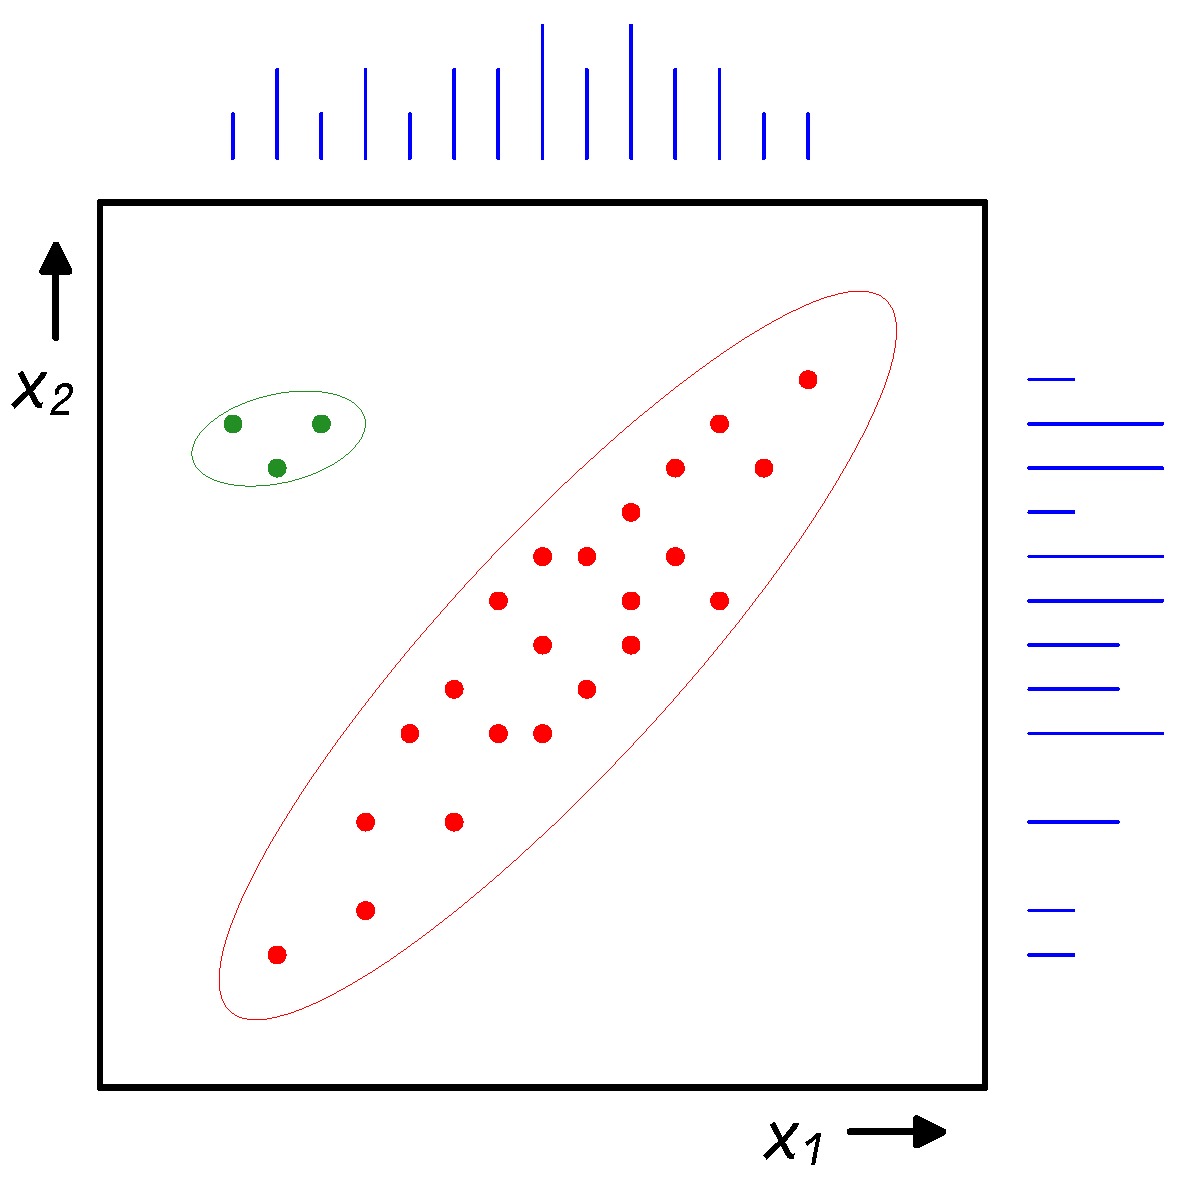
\includegraphics[width=0.75\textwidth]{Graphics/MultivariateNormal}
\end{figure}

Another problem occurs if the data distribution is not multivariate normal. For example, if the data really contain two distinct populations, the centroid calculated will be located between the populations and have no meaning (see fig. \ref{fig:MultNorm}). Of course, \arr{S} would also be meaningless. Methods to detect violation of multivariate normality are discussed in section \ref{text:MulNorm} on page \pageref{text:MulNorm}.

\subsubsection{The multivariate median}

\begin{figure}
 \caption{Two-dimensional example of convex hull stripping. The outermost data are iteratively removed, until only the data of the innermost hull remain, here a single data point. The centroid of this innermost hull is the multivariate median. For details see text.}
 \label{fig:Hull}
 \centering
 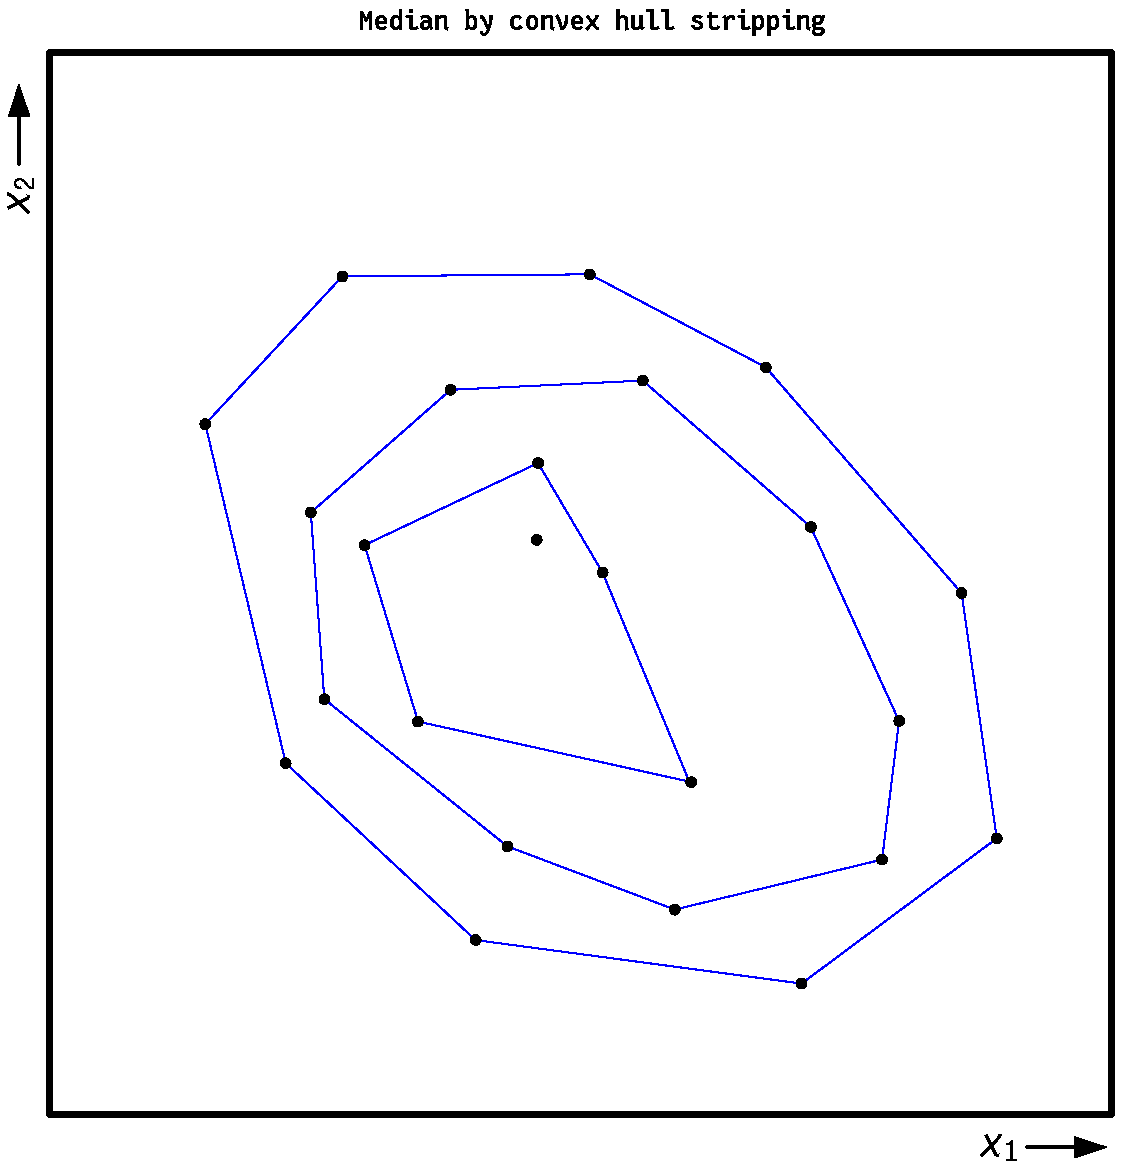
\includegraphics[width=0.75\textwidth]{Graphics/HullStripping}
\end{figure}


A data vector can be sorted, and hence its median determined. For a matrix, this is not possible. Several definitions of the multivariate median are used \parencite{Sma-90}, of which the conceptually most useful are:
\begin{description}
  \item[vector of medians]{is appropriate only if the variables in the data set are orthogonal (uncorrelated, say, after \acs{PCA}). }
  \item[\skalar{\ell 1} Median]{is the point of the data cloud that minimises the sum of the distance to all data points \( \sum_{i=1}^n{||\AbsVec{x}_i - \hat{\mu}||} \) (position of warehouse that optimally supplies all customers). It has a breakdown-point of \SI{50}{\%} and reduces to the standard median in the 1D-case. Unfortunately, there is no efficient algorithm for finding it.}
  \item[convex hull stripping]{For calculation of the univariate median, we recursively remove the largest and smallest values, until we are left with either one value (which is the median) or two (then the median is in between). This idea can be extended to multiple dimensions, by finding the hull of the data cloud. The hull is a convex polygon that encloses all data points with maximal area and minimal circumference. These points are removed, the new hull is calculated and removed and so on, until all remaining points are on the innermost hull. If this innermost hull consists of a single point, this point is the median, otherwise, the centroid is used (see fig. \ref{fig:Hull}).
      However, the breakdown point is \skalar{1/n} under unfavourable circumstances (if all data are on the hull). The median is also not a continuous function of the data in the matrix \arr{X}. }
  \item[Simplicial depth median]{If, in the 1D case, we construct all possible pairs of data points, then the median is the point which is enclosed by the largest number of these intervals, it is \emph{deep inside} the data cloud. This can be extended to \skalar{p} dimensions by replacing the intervals with simplexes \skalar{S(\AbsVec{x}_1, \ldots \AbsVec{x}_{p+1})}. Then
      \begin{equation}
        \mathrm{SDF}(\mu) = \binom{n}{p+1}^{-1} \sum_{1\leq i_1< \ldots < i_{p+1} \leq n}{1[\mu \in S(\AbsVec{x}_1, \ldots \AbsVec{x}_{p+1})]}
      \end{equation}
      Then the simplicial depth median is the point \skalar{\hat{\mu}}, that maximises SDF(\skalar{\mu}).
      }
\end{description}

\section{Test program}

\begin{lstlisting}
  PROGRAM TestDescript;

  USES math, MathFunc, Vector, Matrix, Zufall, Deskript;

  CONST ProbSize = 100;
        Vars     =   2;

  VAR Data, Weights, Dm, Dr       : VectorTyp;
      i, j                        : WORD;
      MinEle, MaxEle, sum, mean,
      std, q1, q2, q3, e2, e3, e4 : float;
      MData, DataWithWeights      : MatrixTyp;

  BEGIN
    CreateVector(Data, ProbSize, 0.0);
    CreateVector(Weights, ProbSize, 1/ProbSize);
    FOR i := 1 TO ProbSize DO
      SetVectorElement(Data, i, 100 + RandomNormal(0, 10));

    Mean := ArithmeticMean(Data);
    Writeln('Arithmetic mean: ', FloatStr(Mean, 10));
    Writeln('Geometric mean: ', FloatStr(GeometricMean(Data), 10));
    Writeln('Harmonic mean: ', FloatStr(HarmonicMean(Data), 10));
    Writeln;
    Writeln('Power mean, k=1: ', FloatStr(GeneralMean(Data, Weights, 1), 10));
    Writeln('Power mean, k=0.001: ', FloatStr(GeneralMean(Data, Weights, 0.001), 10));
    Writeln('Power mean, k=-1: ', FloatStr(GeneralMean(Data, Weights, -1), 10));
    Writeln;
    std := StandardDeviation(Data);
    Writeln('Standard deviation', FloatStr(std, 10));
    Writeln('excess kurtosis', FloatStr(ExcessKurtosis(Data, mean, std), 10));
    Writeln('Skewness', FloatStr(Skewness(Data, mean, std), 10));
    Writeln;
    Writeln('Gini coefficient: ', FloatStr(Gini(Data, Mean), 10));
    Writeln('Herfindahl-Index: ', FloatStr(HerfindahlIndex(Data), 10));
    Writeln;
    q2 := Median(Data);
    q1 := Quantile(Data, 0.25);
    q3 := Quantile(Data, 0.75);
    Writeln('Median: ', FloatStr(q2, 10));
    Writeln('Trimedian: ', FloatStr(Trimedian(Data), 10)); // data have been sorted by Median
    Writeln('Inter-quartile distance: ', FloatStr(InterQuantilDistance(q1, q3), 10));
    Writeln('MAD: ', FloatStr(MAD(Data), 10));
    Writeln('std. error of median: ', FloatStr(StandardErrorOfMedian(Data), 10));
    Writeln;
    Writeln('Naive Hodges-Lehmann: ', FloatStr(NaiveHodgesLehmann(Data), 10),
    ' Hodges-Lehmann estimator: ', FloatStr(HodgesLehmann(Data), 10)); // data have been sorted by Median
    Writeln('Naive Sn: ', FloatStr(NaiveSn(Data), 10), ' Sn: ', FloatStr(Sn(Data), 10));
    Writeln('Naive Qn: ', FloatStr(NaiveQn(Data), 10));
  //  Writeln('Qn: ', FloatStr(Qn(Data), 10));

    FOR i := 1 TO ProbSize DO SetVectorElement(Weights, i, RandomNormal(1/ProbSize, 0.01));
    MaxEle := FindLargest(Weights);
    MinEle := FindSmallest(Weights);
    Scale(Weights, MinEle, MaxEle); // weights IN 0..1
    Sum := TotalSum(Weights);
    FOR i := 1 TO ProbSize DO
      SetVectorElement(Weights, i, GetVectorElement(Weights, i)/Sum); // total weight = 1
    CreateMatrix(DataWithWeights, ProbSize, 2, 0.0);
    SetColumn(DataWithWeights, Data, 1);
    SetColumn(DataWithWeights, Weights, 2);
    Writeln;
    Write('Weighted median: ', FloatStr(WeightedMedian(DataWithWeights), 10));
    Writeln(', weighted LoMed:  ', FloatStr(WeightedLoMed(DataWithWeights), 10),
            ', weighted HiMed:  ', FloatStr(WeightedHiMed(DataWithWeights), 10));
    Writeln;
    e2 := ell2(Data);
    e3 := ell3(Data);
    e4 := ell4(Data);
    Writeln('ell2: ', FloatStr(e2, 10), ', ell3: ', FloatStr(e3, 10), ', ell4: ', FloatStr(e4, 10));
    Writeln('tau2: ', FloatStr(e2/mean, 10), ', tau3: ', FloatStr(e3/e2, 10), ', tau4: ', FloatStr(e4/e2, 10));
    Writeln('Ouartile coefficient of skewness: ', FloatStr(QuartileCoefficientOfSkewness(q1, q2, q3), 10));
    Writeln('Centile coefficient of kurtosis: ', FloatStr(CentilCoeffKurtosis(Data), 10));
    ReadLn;
    DestroyVector(Data);
    DestroyMatrix(DataWithWeights);

    CreateMatrix(MData, ProbSize, Vars, 0.0);
    FOR i := 1 TO (ProbSize DIV 10) DO              // 10% outliers
      BEGIN
        SetMatrixElement(MData, i, 1, 115 + RandomNormal(0, 3));
        SetMatrixElement(MData, i, 2, 110 + RandomNormal(0, 3));
      END;
    FOR i := Succ(ProbSize DIV 10) TO ProbSize DO   // 90% inliers
      BEGIN
        SetMatrixElement(MData, i, 1, 110 + RandomNormal(0, 3));
        SetMatrixElement(MData, i, 2, 115 + RandomNormal(0, 3));
      END;
    RobustDistance (MData, Dr);
    MahalanobisDistance (MData, Dm);
    FOR i := 1 TO ProbSize DO
      Writeln(i:3, ' ', FloatStr(GetMatrixElement(MData, i, 1), 11), ' ',
      FloatStr(GetMatrixElement(MData, i, 2), 11), ' ',
      FloatStr(GetVectorElement(Dm, i), 10), ' ', FloatStr(GetVectorElement(Dr, i), 10));

    ReadLn;
    DestroyVector(Dr);
    DestroyVector(Dm);
    DestroyMatrix(MData);
  END.
\end{lstlisting}

\printbibliography[heading=subbibliography]
\end{refsection}

  % -*- TeX:UK -*-
\chapter{Correlation coefficients}
\begin{refsection}
\label{text:correlation}

\abstract{If \skalar{k} variables are observed in an experiment, then we get a \(k\times\ k \) matrix \arr{R} of correlation coefficients \skalar{r} between these variables. The diagonal elements are always \num{1.0}, as each variable correlates perfectly with itself. Also, for all \skalar{i,j} \(\skalar{r}_{i,j} = \skalar{r}_{j,i} \), \Foreign{i.e.}, \arr{R} is symmetrical. There are different ways to calculate the correlation coefficients, depending on the scale level of the data.}

The unit calculates various types of correlation coefficients. Missing data should be encoded \acs{NaN}. Nominal, binary and ordinal values are given as integer numbers, but in vectors and fields of type double (alternatively, the type definitions in units Vector and Matrix would have to be overloaded).

The record Significance contains the appropriate test variable, degrees of freedom and probability for \(\mathbf{H_0}: r = 0 \) \Foreign{vs} \(\mathbf{H_1}: r \neq\ 0 \)

\begin{table}
  \caption{Interpretation of correlation coefficients.}
  \label{tab:intlam}
  \centering
    \begin{tabular}{ll}
      \toprule
      \skalar{|r|} & meaning                   \\
      \midrule
     .00 to .19    & little to no relationship \\
     .20 to .39    & weak relationship         \\
     .40 to .59    & moderate relationship     \\
     .60 to .79    & strong relationship       \\
     .80 to 1.0    & very strong relationship  \\
      \bottomrule
    \end{tabular}
\end{table}

\begin{lstlisting}[caption=Interface for unit Correlations]
INTERFACE

USES Math, MathFunc, Vector, Stat, Deskript;

CONST
  MaxCases = 1360;
  MaxSteps = 100; // maximal # OF different values FOR ordinal AND nominal data
  CorrelationsError: BOOLEAN = FALSE;

TYPE
  ContStruc = RECORD
    Table: ARRAY [0..MaxSteps, 0..MaxSteps] OF WORD;
    RowSums, ColumnSums: ARRAY [0..MaxSteps] OF WORD;
    r, c, n: WORD;
    // number OF rows, columns AND legal (no NaN) comparisons
  END;
  ContTable = ^ContStruc;

  Confusion = RECORD
    a, b, c, d: WORD;
  END;

  SignificanceType = RECORD
    TestValue, Freedom, P0: float;
  END;

PROCEDURE CorrelationSignificance(CONST Vector1, Vector2: VectorTyp;
  r: float; VAR Significance: SignificanceType);

FUNCTION PearsonProductMomentCorrelation(CONST Vector1, Vector2: VectorTyp;
  VAR Significance: SignificanceType): float;

FUNCTION WeightedPearson(CONST Vector1, Vector2, weight: VectorTyp;
  VAR Significance: SignificanceType): float;

PROCEDURE Rank(VAR Data: VectorTyp);

FUNCTION SpearmanRankCorrelation(CONST Vector1, Vector2: VectorTyp;
  VAR Significance: SignificanceType): float;

FUNCTION QuadrantCorrelation(CONST Vector1, Vector2: VectorTyp;
  VAR Significance: SignificanceType): float;

FUNCTION PointBiserialCorrelation(CONST BinaryVector, CardinalVector: VectorTyp;
  VAR Significance: SignificanceType): float;

FUNCTION ConfusionTable(CONST Vector1, Vector2: VectorTyp): Confusion;

FUNCTION McConnaugheyCorrelation(c: confusion): float;

FUNCTION MatthewsCorrelation(c: Confusion): float;

FUNCTION Rk(Cont: ContTable): float;

PROCEDURE Contingency(Data1, Data2: VectorTyp; VAR Cont: ContTable);

PROCEDURE WriteContingency(CONST Cont: ContTable; MedStr: STRING; ValidFigures: BYTE);

PROCEDURE DestroyContingency(VAR Cont: ContTable);

FUNCTION Chi2(CONST Contingency: ContTable;
  VAR Significance: SignificanceType): float;

FUNCTION Phi2(CONST Contingency: ContTable;
  VAR Significance: SignificanceType): float;

FUNCTION CramersVTilde(chi2: float; r, c, n: WORD): float;

FUNCTION lambda(CONST Contingency: ContTable): float;

FUNCTION lambda_r(CONST Contingency: ContTable): float;

FUNCTION lambda_c(CONST Contingency: ContTable): float;

FUNCTION OrdinalCorrelations(CONST Data1, Data2: VectorTyp; Formula: CHAR;
  VAR Significance: SignificanceType): float;

FUNCTION theta(CONST Contingency: ContTable): float;

FUNCTION eta_sqr(CONST NominalVector, CardinalVector: VectorTyp;
  VAR Significance: SignificanceType): float;

{ ************************* calculations with r ***************************** }

FUNCTION AverageCorrelations(CONST Correlations: VectorTyp): float;

FUNCTION Angle(r: float): float;


IMPLEMENTATION
\end{lstlisting}

One thing to remember about all correlation coefficients: \textbf{Correlation does not prove causality}! This is known as the \Foreign{cum hoc, ergo propter hoc} fallacy. If a correlation is found between two variables \AbsVec{x,y}, then there are several possible explanations:
\begin{description}
  \item[direct causation]{\AbsVec{x} causes \AbsVec{y}}
  \item[reverse causation]{\AbsVec{y} causes \AbsVec{x}}
  \item[cyclic causation]{\AbsVec{x} causes \AbsVec{y} and \AbsVec{y} causes \AbsVec{x}}
  \item[indirect causation]{\AbsVec{x} causes \AbsVec{a}, which causes \AbsVec{y}}
  \item[common cause]{Both \AbsVec{x,y} are caused by another (\textbf{confounding}) factor. Many such pseudo-correlations have been published, including between polio incidence and ice cream sales (polio virus is spread by the fecal-oral route in swimming pools, hence mostly in warm weather when ice cream sales also increase) or human birth rate and number of storks (\parencite{Sie-88}, both decline with industrialisation).}
  \item[coincidence]{the correlation is spurious and will vanish if new data become available.}
\end{description}

Correlation coefficients may be symmetrical (\( -1 \leq r \leq +1 \)) or unsymmetrical (\( 0 \leq r^* \leq +1 \)). A symmetrical coefficient can be converted to unsymmetrical by \( r^* = 0.5 (r +1) \) and \Foreign{vice versa} by \( r = 2r^* - 1 \).

\section{General routines}

\begin{lstlisting}[caption=Test for equal vector length ]
  FUNCTION TestDataVectorLength(Data1, Data2: VectorTyp): BOOLEAN;

  BEGIN
    IF (VectorLength(Data1) <> VectorLength(Data2))
      THEN
        BEGIN
          c := WriteErrorMessage(' Correlation: vectors of unequal length');
          Result := FALSE;
        END
      ELSE
        Result := TRUE;
  END;
\end{lstlisting}

\begin{lstlisting}[caption= Average of several correlation coefficients ]
  FUNCTION AverageCorrelations(CONST Correlations: VectorTyp): float;

  VAR
    i, j, k: WORD;
    SumR: float;

  BEGIN
    k := VectorLength(Correlations);
    SumR := 0;
    j := 0;
    FOR i := 1 TO k DO
      IF IsNaN(GetVectorElement(Correlations, i))
        THEN // ignore
        ELSE
          BEGIN
            SumR := SumR + tanh(GetVectorElement(Correlations, i));
            Inc(j);
          END;
    Result := arctanh(SumR / j);
  END;
\end{lstlisting}


\section{Cardinal (interval and rational) data}

\subsection{\Name{Pearson}'s product moment correlation coefficient \(r_p \)}\label{text:Pearson}

In common usage, when we speak of a correlation coefficient without further specification, then \Name{Pearson}'s product moment coefficient \skalar{r_p} \parencite{Pea-95} is meant. However, it is defined only for data on a interval or rational scale, it has also been used for binary data. For two data vectors \AbsVec{x} and \AbsVec{y}, both of length \skalar{n}, \skalar{r_p} is
\begin{equation}
  r_p = \frac{\sum_{i=1}^n{(\AbsVec{x}_i - \bar{\AbsVec{x}}) \sum_{i=1}^n{(\AbsVec{y} - \bar{\AbsVec{y}})}}}{\sqrt{\sum_{i=1}^n{(\AbsVec{x}_i - \bar{\AbsVec{x}})^2 \sum_{i=1}^n{(\AbsVec{y}_i - \bar{\AbsVec{y}})^2}}}} = \frac{n \sum_{i=1}^n{(\AbsVec{x}_i \AbsVec{y}_i)} - \sum_{i=1}^n{\AbsVec{x}_i} \sum_{i=1}^n{\AbsVec{y}_i}}{\sqrt{[n \sum_{i=1}^n{\AbsVec{x}_i^2} - (\sum_{i=1}^n{\AbsVec{x}_i})^2] [n \sum_{i=1}^n{\AbsVec{y}_i^2} - (\sum_{i=1}^n{\AbsVec{y}_i})^2]}}
\end{equation}
Computationally, the second way to calculate \skalar{r_p} is quicker, as it doesn't require the calculation of averages, that is, the loop over all \AbsVec{x}, \AbsVec{y} has to be done only once, not twice.

\begin{lstlisting}[caption= \Name{Pearson} product moment correlation]
  FUNCTION PearsonProductMomentCorrelation(CONST Vector1, Vector2: VectorTyp;
    VAR Significance: SignificanceType): float;

  VAR
    i, j: WORD;
    SumXY, SumX, SumY, SumX2, SumY2, varX, varY, covXY, x, y, r: float;

  BEGIN
    IF NOT (TestDataVectorLength(Vector1, Vector2)) THEN EXIT;
    SumXY := 0;
    SumX := 0;
    SumY := 0;
    SumX2 := 0;
    SumY2 := 0;
    j := 0;
    FOR i := 1 TO VectorLength(Vector1) DO
      BEGIN
        x := GetVectorElement(Vector1, i);
        y := GetVectorElement(Vector2, i);
        IF (IsNaN(x) OR IsNaN(y))
          THEN // ignore
          ELSE
            BEGIN
              SumXY := SumXY + x * y;
              SumX := SumX + x;
              SumY := SumY + y;
              SumX2 := SumX2 + x * x;
              SumY2 := SumY2 + y * y;
              INC(j); // actual number OF valid comparisons
            END; { else }
      END; { for }
    varX := j * SumX2 - SumX * SumX;
    varY := j * SumY2 - SumY * SumY;
    covXY := j * SumXY - SumX * SumY;
    IF (varX * varY) = 0
      THEN r := 0     // ???
      ELSE r := covXY / Sqrt(varX * varY);
    CorrelationSignificance(Vector1, Vector2, r, Significance);
    Result := r;
  END; { PearsonProductMoment }
\end{lstlisting}

For factor analysis the data should be \skalar{z}-standardised \( \bar{x} = 0, \sigma = 1 \)) before calculating the correlation coefficient, especially if they have widely varying scales. Otherwise, factor analysis may pick the variable that has the highest variance as the direction of the greatest variability. Then
\begin{equation}
  \AbsVec{z}_i = \frac{\AbsVec{x}_i - \bar{\AbsVec{x}}}{\sigma}
\end{equation}

It is possible to weigh data points by importance (\Foreign{e.g.}, relative standard deviations if they are means) with a weight vector \AbsVec{w}:
\begin{align}
  \bar{\AbsVec{x}}  & = \frac{\sum_{i=1}^n{\AbsVec{w}_i \AbsVec{x}_i}}{\sum_{i=1}^n{\AbsVec{w}_i}} \quad \bar{\AbsVec{y}}    = \frac{\sum_{i=1}^n{\AbsVec{w}_i \AbsVec{y}_i}}{\sum_{i=1}^n{\AbsVec{w}_i}} \\
  s_{x,y}           & = \frac{\sum_{i=1}^n{\AbsVec{w}_i (\AbsVec{x}_i - \bar{\AbsVec{x}}_i) (\AbsVec{y}_i - \bar{\AbsVec{y}}_i)}}{\sum_{i=1}^n{\AbsVec{w}_i}} \quad
                  s_x^2 = \frac{\sum_{i=1}^n{\AbsVec{w}_i (\AbsVec{x}_i - \bar{\AbsVec{x}})^2}}{\AbsVec{w}_i} \quad
                  s_y^2 = \frac{\sum_{i=1}^n{\AbsVec{w}_i (\AbsVec{y}_i - \bar{\AbsVec{y}})^2}}{\AbsVec{w}_i} \\
  r(\AbsVec{x,y,w}) & = \frac{s_{x,y}}{\sqrt{s_x^2 s_y^2}}
\end{align}

\begin{lstlisting}[caption=Weighted \Name{Pearson} product moment correlation]
  FUNCTION WeightedPearson(CONST Vector1, Vector2, weight: VectorTyp;
    VAR Significance: SignificanceType): float;

  VAR
    i, n: WORD;
    BarX, BarY, SumWX, SumWY, SumW, r, SumWXd, SumWYd, SumWXYd, CovXY,
    VarX, VarY, x, y, w: float;

  BEGIN
    IF NOT (TestDataVectorLength(Vector1, Vector2)) THEN EXIT;
    n := VectorLength(Vector1);
    SumWX := 0;
    SumWY := 0;
    SumW := 0;
    SumWXd := 0;
    SumWYd := 0;
    SumWXYd := 0;
    FOR i := 1 TO n DO
      BEGIN
        x := GetVectorElement(Vector1, i);
        y := GetVectorElement(Vector2, i);
        w := GetVectorElement(Weight, i);
        IF (IsNaN(x) OR IsNaN(x) OR IsNaN(w))
          THEN // ignore
          ELSE
            BEGIN
              SumWX := SumWX + w * x;
              SumWY := SumWY + w * y;
              SumW := SumW + w;
            END; { else }
      END; { for }
    BarX := SumWX / SumW;     // calculate averages
    BarY := SumWY / SumW;
    FOR i := 1 TO n DO
      BEGIN
        x := GetVectorElement(Vector1, i);
        y := GetVectorElement(Vector2, i);
        w := GetVectorElement(Weight, i);
        IF (IsNaN(x) OR IsNaN(y) OR IsNaN(w))
          THEN  // ignore
          ELSE
            BEGIN
              SumWXd := SumWXd + w * (x - BarX) * (x - BarX);
              SumWYd := SumWYd + w * (y - BarY) * (y - BarY);
              SumWXYd := SumWXYd + w * (x - BarX) * (y - BarY);
            END; { else }
      END; { for }
    CovXY := SumWXYd / SumW;
    VarX := SumWXd / SumW;
    VarY := SumWYd / SumW;
    IF (varX * varY) = 0
      THEN r := 0   // ???
      ELSE r := CovXY / Sqrt(VarX * VarY);
    CorrelationSignificance(Vector1, Vector2, r, Significance);
    Result := r;
  END; { WeightedPearson }
\end{lstlisting}

The standard error of \skalar{r_p} is
\begin{equation}
  \sigma = \frac{0.6325}{\sqrt{n-1}}
\end{equation}
To test for the 0-hypothesis \(r_p = 0 \) even for small data sets use
\begin{equation}
  \label{eqn:rt-sig}
  t = r_p \sqrt{\frac{n-2}{1-r_p^2}}\quad \nu = n-2
\end{equation}
for \(r < 1 \).

\begin{lstlisting}[caption=Probability for r = 0]
  PROCEDURE CorrelationSignificance(CONST Vector1, Vector2: VectorTyp;
    r: float; VAR Significance: SignificanceType);

  VAR
    i, n, m: WORD;

  BEGIN
    n := VectorLength(Vector1);
    IF NOT (TestDataVectorLength(Vector1, Vector2))
      THEN EXIT;
    m := 0;
    FOR i := 1 TO n DO
      IF (IsNaN(GetVectorElement(Vector1, i)) OR IsNaN(GetVectorElement(Vector1, i)))
        THEN // ignore
        ELSE INC(m);
    Significance.TestValue := (m - 2) / (1 - r * r);
    IF signum(Significance.TestValue) >= 0
      THEN Significance.TestValue := r * Sqrt(Significance.TestValue)
      ELSE Significance.TestValue := 0;
    Significance.Freedom := m - 2;
    Significance.P0 := Integral_t(Significance.TestValue, Round(Significance.Freedom));
  END;
\end{lstlisting}

To compare the difference of two \skalar{r}-values for significance (if for both data sets \(n \geq 10 \)) \Name{Fisher}'s \skalar{z}-transformation is used for both coefficients:
\begin{equation}
  z_i = 0.5 \ln\left(\frac{1+r_i}{1-r_i}\right)
\end{equation}
The two-sided significance of the difference is
\begin{equation}
  P_0 = \mathrm{erfc}\left(\frac{|z_1 - z_2|}{\sqrt{2} \sqrt{\frac{1}{n_1 -3} + \frac{1}{n_2 - 3}}}\right)
\end{equation}

To compare an observed \skalar{r_o} with a hypothetical value \skalar{r_h}, use
\begin{align}
  z_h & = 0.5 * \left[\ln\left(\frac{1 + r_h}{1-r_h}\right) + \frac{r_h}{n-1}\right] \\
  P(0)    & = \mathrm{erfc}\left(\frac{|z - z_h| \sqrt{n-3}}{\sqrt{2}}\right)
\end{align}

\skalar{n} correlation coefficients can be averaged only after transformation:
\begin{equation} \label{eqn:AvCorr}
  \bar{r} = \tanh^{-1}\left(\frac{\sum_{i=1}^n{\tanh(\skalar{r}_i)}}{n}\right)
\end{equation}

\subsubsection{Geometric and PRE interpretation of \Name{Pearson}'s correlation coefficient}

For \skalar{n} samples of a random variable \(\arr{Y} = (\AbsVec{y}_1, \AbsVec{y}_2, \ldots \AbsVec{y}_n) \) the expected value of \arr{Y} is \parencite{Gni-13}
\begin{equation}
  \mu = E(\arr{Y}) = \sum_{j=1}^p{\AbsVec{y}_j \AbsVec{p}_j}
\end{equation}
with \(\AbsVec{p}_i \) the probability of the \skalar{i}-th element. Then the arithmetic mean \(\bar{\AbsVec{y}} \) is an estimator of this expected value:
\begin{equation}
  \bar{\AbsVec{y}} = \frac{1}{n} \sum_{i=1}^n{\AbsVec{y}_i}
\end{equation}
and the variance is a measure of scatter around the expected value:
\begin{equation}
  \sigma(\arr{Y}) = E[(\arr{Y}-\mu)^2] = \sum_{i=1}^n{(\AbsVec{y}_i-\mu)^2 \AbsVec{p}_i}
\end{equation}
and its estimator is
\begin{equation}
  s^2 = \frac{1}{n-1} \sum_{i=1}^n{(\AbsVec{y}_i - \bar{\AbsVec{y}})}
\end{equation}
and its square root is the standard deviation \skalar{s} (which has the same unit as \arr{Y}). If one had to guess a \(\AbsVec{y}_i \), then the best estimator would be \(\bar{\AbsVec{y}} \) and \skalar{s} would be the probable error.

Then a measure of the relationship of two variables \arr{X,Y} is their covariance
\begin{equation}
  \sigma_{\arr{X,Y}} = E[(\arr{X} -\mu_\arr{X})(\arr{Y} - \mu_\arr{Y})]
\end{equation}
which when normalised to unity is \Name{Pearson}'s correlation coefficient \skalar{r_p}:
\begin{equation}
  r_p = \frac{\sigma_\arr{X,Y}}{\sigma_\arr{X} \times\ \sigma_\arr{Y}}
      = \frac{E[(\arr{X} -\mu_\arr{X})(\arr{Y} - \mu_\arr{Y})]}{E[(\arr{X}-\mu_\arr{X})^2] \times\  E[(\arr{Y}-\mu_\arr{Y})^2]}
      = \frac{\sum_{i=1}^n{[(\AbsVec{x}_i - \bar{\AbsVec{x}}) (\AbsVec{y}_i - \bar{\AbsVec{y}})]}}{\sqrt{\sum_{i=1}^n{(\AbsVec{x}_i - \bar{\AbsVec{x}})^2}} \sqrt{\sum_{i=1}^n{(\AbsVec{y}_i - \bar{\AbsVec{y}})^2}}}
\end{equation}
The dispersion of a random variable is \(\tilde{\AbsVec{x}}_i = \AbsVec{x}_i - \bar{\AbsVec{x}} \). Using this we can write
\begin{equation} \label{eqn:corr1}
  r_p = \frac{\sum_{i=1}^n{\tilde{\AbsVec{x}}_i \tilde{\AbsVec{y}}_i}}{\sqrt{\sum_{i=1}^n{\tilde{\AbsVec{x}}_i}} \times\ \sqrt{\sum_{i=1}^n{\tilde{\AbsVec{y}}_i}}}
\end{equation}

A variable \arr{X} can be interpreted as a vector in \skalar{p}-dimensional space. The \Name{Euklid}ian norm (length) of this vector is
\begin{equation} \label{eqn:norm}
  |\arr{X}| = \sqrt{\sum_{i=1}^n{\AbsVec{x}_i^2}}
\end{equation}
The dot product of two such vectors of equal length is
\begin{equation}
  \arr{X} \bullet \arr{Y} = \sum_{i=1}^{n}{\AbsVec{x}_i \AbsVec{y}_i} = |\arr{X}| \times\ |\arr{Y}| \times\ \cos{(\arr{X} \arr{Y})}
\end{equation}
with \(\cos{(\arr{X} \arr{Y})} \) the cosine of the angle between the vectors, which in other words is equal to
\begin{equation}
  \cos{(\arr{X} \arr{Y})} = \frac{\arr{X} \bullet \arr{Y}}{|\arr{X}| \times\ |\arr{Y}|}
\end{equation}
Using eqn. \ref{eqn:corr1}, we see that
\begin{equation} \label{eqn:cosine}
    r_p = \frac{\sum_{i=1}^n{\tilde{\AbsVec{x}}_i \tilde{\AbsVec{y}}_i}}{\sqrt{\sum_{i=1}^n{\tilde{\AbsVec{x}}_i}} \times\ \sqrt{\sum_{i=1}^n{\tilde{\AbsVec{y}}_i}}} = \frac{\arr{X} \bullet \arr{Y}}{|\arr{X}| \times\ |\arr{Y}|} = \cos{(\arr{X} \arr{Y})}
\end{equation}
the correlation coefficient \skalar{r_p} is equal to the cosine of the angle between the data vectors \arr{X,Y}. If \skalar{r_p} is zero, the angle between the vectors is \ang{90} and the data are independent. If \skalar{r_p} is unity, the angle is \ang{0} and the vectors are parallel and the data are perfectly correlated.

\begin{lstlisting}[caption= Convert correlation to angle]
  FUNCTION Angle (r : float) : float;

  BEGIN
     Result := ArcCos(r) * 180 / Const_pi;
  END;
\end{lstlisting}

Now consider the situation that we had two random variables \arr{X,Y} which are related by a linear regression line
\begin{equation}
  \hat{\arr{Y}} = a + b \times\ \arr{X}
\end{equation}
Then the correlation coefficient is
\begin{equation} \label{eqn:corr2}
  r_p = \frac{\sum_{i=1}^n{[(\AbsVec{y}_i - \bar{\AbsVec{y}}) \times\ (\hat{\AbsVec{y}}_i - \bar{\AbsVec{y}}) ]}}{\sqrt{\sum_{i=1}^n{(\AbsVec{y}_i - \bar{\AbsVec{y}})^2} \times \sum_{i=1}^n{(\hat{\AbsVec{y}}_i - \bar{\AbsVec{y}})^2}}}
\end{equation}
which again is equal to the cosine of two vectors, representing the dispersion of \arr{Y} and \(\hat{\arr{Y}} \), respectively. Eqn. \ref{eqn:corr2} can also be written as
\begin{equation}
  r_p = \frac{\sqrt{\sum_{i=1}^n{(\hat{\AbsVec{y}}_i - \bar{\AbsVec{y}})^2}}}{\sqrt{\sum_{i=1}^n{(\AbsVec{y}_i - \bar{\AbsVec{y}})^2}}}
\end{equation}
which is the ratio of the length of the two vectors.

If \(SS_\mathrm{total} = \sum{(\AbsVec{y}_i - \bar{\AbsVec{y}})^2} \), \(SS_\mathrm{explained} = \sum{(\hat{\AbsVec{y}}_i - \bar{\AbsVec{y}})^2} \) and \(SS_\mathrm{residual} = \sum{(\AbsVec{y}_i - \hat{\AbsVec{y}}_i)^2} \), then \(r^2 = 1 - \frac{SS_\mathrm{residual}}{SS_{total}} \) the \textbf{coefficient of determination}, that is, the part of the variance in \AbsVec{y} that is explained by the regression equation. Thus, \skalar{r_p^2} is a \textbf{proportional reduction in error (PRE)} measure, which is determined by how much error is reduced if for any \(\AbsVec{x}_i \) one uses \(\hat{\AbsVec{y}}_i \) instead of \(\bar{\AbsVec{y}} \) to predict \(\AbsVec{y}_i \) \parencite{Cos-65}.

Although some of the other correlation coefficients discussed below have a PRE interpretation, the angle interpretation is specific to \skalar{r_p}.

\subsubsection{Partial correlation}

If the correlation between two variables \AbsVec{X, Y} is caused by the effect of a third \AbsVec{Z} on both, then this can be detected with the partial correlation coefficient
\begin{equation}
  r_{\AbsVec{XY}|\AbsVec{Z}} = \frac{r_{\AbsVec{XY}} - r_{\AbsVec{XZ}} \times r_{\AbsVec{YZ}}}{\sqrt{(1-r_\AbsVec{XZ}^2)(1-r_\AbsVec{YZ}^2)}}
\end{equation}

The partial correlation can also be used to determine if a particular variable out of a set of independent variables contributes to the explanatory power of that set towards a dependent variable. It simply compares the sum of squared errors \(\mathsf{SS}_\mathrm{res} = \sum_{i=1}^{n}(\AbsVec{y}_i - \hat{\AbsVec{y}}_i)^2 \) for the full and the reduced model (that is, model without the variable under test):
\begin{equation}
  r^2_\mathrm{par} = \frac{\mathsf{SS}_\mathrm{res, red} - \mathsf{SS}_\mathrm{res, full}}{\mathsf{SS}_\mathrm{res, red}} = \frac{r^2_\mathrm{full} - r^2_\mathrm{red}}{1 - r^2_\mathrm{red}}
\end{equation}

\subsubsection{Limitations of \Name{Pearson}'s \skalar{r_p}}

\Name{Pearsons}'r \skalar{r_p} is not a robust estimate of the association between two variables. It is affected by outliers, heteroscedasticity, curvature, the magnitude of residuals and range restriction \parencite[fig. 2]{Per-13}. Many such pitfalls can be detected by plotting the data!

Relatively large \skalar{n} (\( > 100 \)) is required for the sample \skalar{r} to be a reliable estimate for the population \skalar{r}, especially when the ``true'' correlation is small. If \(n < 30 \) and the measured \(r > 0.6 \), then a correction should be applied to the correlation coefficient \parencite{Olk-58}, because the sample \skalar{r} tends to underestimate the population association:
\begin{equation}
  r^* = r \left(1 + \frac{1 - r^2}{2 (n-3)}\right)
\end{equation}
, but that is usually ignored.



\subsection{\Name{Spearman}'s rank correlation coefficient \(r_s \)}

\begin{figure}
   \caption{The synthetic data in this plot follow the \Name{Henri-Michaelis-Menten}-law, and the rank correlation coefficient \skalar{r_s} is \num{1.0}. However, because of the curvature of the data, the product moment correlation \skalar{r_p} is only \num{0.73}.}
   \label{fig:Corr}
   \centering
      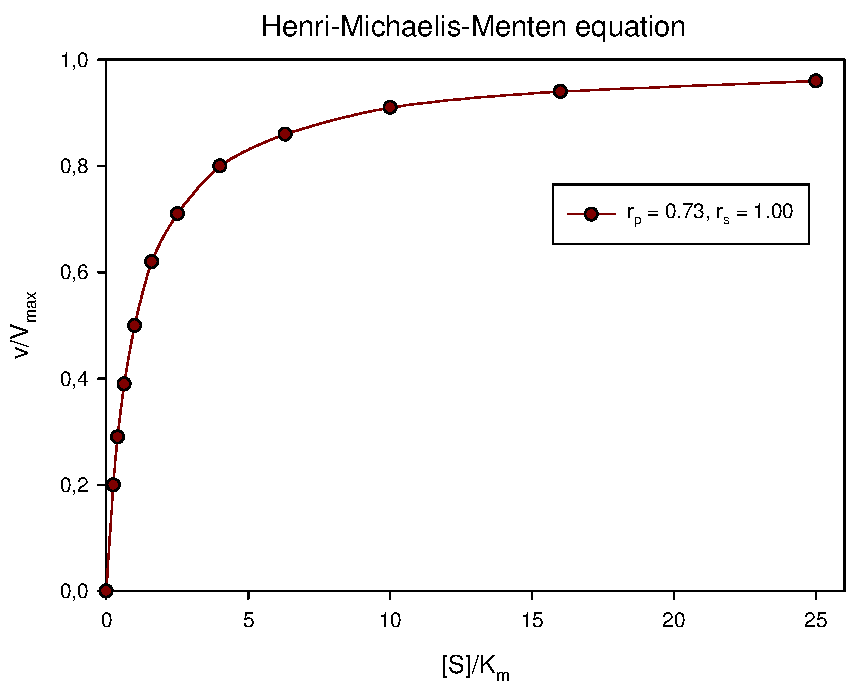
\includegraphics[width=0.75\textwidth]{Graphics/Correlation}
\end{figure}

\skalar{r_s} (\parencite{Spe-04}, often called \textrho) was developed for ordinal scaled variables, however, it can also be used for interval and rational scales. In that case, we work with the rank of each \( \AbsVec{x}_i, \AbsVec{y}_i \) rather than their values. This has the disadvantage of some loss of information, but the advantage that \skalar{r_s} works for non-linear relationships between \AbsVec{x} and \AbsVec{y}, provided only that \AbsVec{y} is a monotonically increasing function of \AbsVec{x} (see fig. \ref{fig:Corr}). For the rank correlation of a linear and a circular variable see chapter \ref{text:circular}.


\begin{lstlisting}[caption=Ranking of a variable]
  PROCEDURE Rank(VAR Data: VectorTyp);

  LABEL
    done;

  VAR
    i, j, k, Valid, n: WORD;
    r, x, y: float;
    Sorted: VectorTyp;

  BEGIN
    n := VectorLength(Data);
    CopyVector(Data, Sorted);
    ShellSort(Sorted);            // create a sorted Copy OF data  (any NaNs TO highest #)
    Valid := n;
    FOR i := 1 TO n DO
      IF IsNaN(GetVectorElement(Sorted, i))
        THEN DEC(Valid);         // determine number OF non-NaN data points
    i := 1;
    REPEAT
      x := GetVectorElement(Sorted, i);
      IF IsNaN(x)
        THEN
        ELSE
          BEGIN
            j := i;
            REPEAT             // find number OF Elements that are equal TO x
              y := GetVectorElement(Sorted, Succ(j));
              IF IsNaN(y)
                THEN GOTO Done // leave counting LOOP, no more valid data
                ELSE IF (x = y)
                       THEN INC(j);
            UNTIL ((x < y) OR (j = n));
  Done:     r := (1.0 * i + j) / 2;     // rank IS average OF lowest + highest element
            FOR k := 1 TO Valid DO      // change all elements OF Data equal TO x -> rank
              BEGIN
                y := GetVectorElement(Data, k);
                IF IsNaN(y)
                  THEN
                  ELSE IF (y = x)
                         THEN SetVectorElement(Data, k, r);
              END;
            i := Succ(j);
          END;
    UNTIL (i >= Valid) OR IsNaN(x);
    DestroyVector(Sorted);
  END;
\end{lstlisting}

The distribution of \skalar{r_s} does not depend on the distribution of \AbsVec{x,y}, so the tests described for \skalar{r_p} can always be used (\skalar{r_s} is non-parametric). The calculation of \skalar{r_s} is performed exactly as described for \skalar{r_p}.

If there are no ties (all x-values different from each other and all y-values different from each other), then there is a computationally simpler form to calculate \skalar{r_s}:
\begin{equation}
  r_s = 1 - \frac{6 \sum_{i=1}^n{(\AbsVec{x}_i - \AbsVec{y}_i)^2}}{n^3-n}
\end{equation}
\skalar{r_s} has no PRE interpretation \parencite{Fre-86}.

\begin{lstlisting}[caption=\Name{Spearman}'s rank correlation coefficient]
  FUNCTION SpearmanRankCorrelation(CONST Vector1, Vector2: VectorTyp;
    VAR Significance: SignificanceType): float;

  VAR
    Ranked1, Ranked2: VectorTyp;

  BEGIN
    IF NOT (TestDataVectorLength(Vector1, Vector2)) THEN EXIT;
    CopyVector(Vector1, Ranked1);
    CopyVector(Vector2, Ranked2);
    Rank(Ranked1);
    Rank(Ranked2);
    Result := PearsonProductMomentCorrelation(Ranked1,
      Ranked2, Significance);
    DestroyVector(Ranked1);
    DestroyVector(Ranked2);
  END;
\end{lstlisting}

\subsubsection{Significance testing of \skalar{r_s}}

A non-zero \skalar{r_s} can be tested for significance by
\begin{equation}
  t = r_s \times \sqrt{\frac{n-2}{1-r_s^2}}
\end{equation}
with \(n-2 \) degrees of freedom.

\subsection{Quadrant correlation \skalar{r_q}}\label{text:quadrant}

The quadrant correlation is measure of correlation robust against outliers. It is calculated from the number of observations in the four quadrants determined by the median pair. The number of observations in quadrant I and III (\skalar{n_+}) and in quadrants II and IV (\skalar{n_-}) are determined:
\begin{equation}
  r_q = \frac{n_+ - n_-}{n_+ + n_-}  = \frac{1}{N} \times \sum_{i=1}^n{\sgn{(\AbsVec{x}_i - \tilde{x})} \times \sgn{(\AbsVec{y}_i - \tilde{y})}}
\end{equation}
with \(\tilde{x},\tilde{y} \) the medians of \AbsVec{X,Y}.

\subsubsection{Median test for significance of \skalar{r_q}}

for the test \(H_0 : r_q = 0 \) \Foreign{vs} \(H_1 : r_q \neq 0 \) calculate (with \(n_e = (n_+ + n_-)/2 \), \(n_e > 5 \)):
\begin{equation}
  \chi^2 \approx \frac{(n_+ - n_e)^2 + (n_- - n_e)^2}{n_e}
\end{equation}
with one degree of freedom.

\begin{lstlisting}[caption=Quadrant correlation and its significance]
  FUNCTION QuadrantCorrelation(CONST Vector1, Vector2: VectorTyp;
    VAR Significance: SignificanceType): float;

  VAR
    Sorted1, Sorted2            : VectorTyp;
    n, i, n_plus, n_minus       : WORD;
    Median1, Median2, x, y, n_e : float;
    c                           : char;

  BEGIN
    IF NOT (TestDataVectorLength(Vector1, Vector2)) THEN EXIT;
    n := VectorLength(Vector1);
    CopyVector(Vector1, Sorted1);
    CopyVector(Vector2, Sorted2);
    Median1 := Median(Sorted1);
    Median2 := Median(Sorted2);
    DestroyVector(Sorted1);
    DestroyVector(Sorted2);
    n_plus := 0;
    n_minus := 0;
    FOR i := 1 TO n DO
      BEGIN
        x := GetVectorElement(Vector1, i);
        y := GetVectorElement(Vector2, i);
        IF IsNaN(x) OR IsNaN(y)
          THEN // ignore NaNs
          ELSE IF ((x = Median1) OR (y = Median2))
                 THEN // ignore data ON coordinate axis OF system WITH origin Median1/Median2
                 ELSE IF (((x > Median1) AND (y > Median2)) OR ((x < Median1) AND (y < Median2)))
                        THEN INC(n_plus)   // concordance: quadrant I OR III
                        ELSE INC(n_minus); // discordance: quadrant II OR IV
      END;
    Result := (n_plus - n_minus) / (n_plus + n_minus);
    n_e := 1.0 * (n_plus + n_minus) / 2;
    IF (n_e < 5)
      THEN
        BEGIN
          c := WriteErrorMessage(' Quadrant correlation: cannot calculate significance because n_e < 5');
          CorrelationsError := TRUE;
          EXIT;
        END;
    Significance.TestValue := ((n_plus - n_e) * (n_plus - n_e) +
      (n_minus - n_e) * (n_minus - n_e)) / n_e;
    Significance.Freedom := 1;
    Significance.P0 := IntegralChi(Significance.TestValue, Round(Significance.Freedom));
  END;
\end{lstlisting}

\section{Binary data}

Association and similarity coefficients for binary data have been reviewed in \parencite{Hub-82}.
Given the confusion table \label{tab:binary}
\begin{tabular}{c|cc}
\toprule
\textsubscript{observed}\textsuperscript{predicted}  & 1 & 0 \\
\midrule
1 & \textcolor{DarkGreen}{TP = a} & \textcolor{DarkRed}{FN = b}   \\
0 & \textcolor{DarkRed}{FP = c}   & \textcolor{DarkGreen}{TN = d} \\
\bottomrule
\end{tabular}\\
the association measure \skalar{r} should meet the following obligatory conditions:
\begin{enumerate}
  \item{For an association measure \(\skalar{r}_{i,j} \leq \skalar{r}_{i,i} \) for all \skalar{i,j} and if \(\skalar{r}_{i,j} > \skalar{r}_{k,l} \) then items \skalar{i,j} are more similar than items \skalar{k,l}.  }
  \item{min(\skalar{r}) should be at \(a = d = 0 \) and max(\skalar{r}) at \(b = c = 0 \).}
  \item{Symmetry: \(\skalar{r}_{i,j} = \skalar{r}_{j,i} \) for all \skalar{i,j}.}
  \item{Discrimination between positive and negative association: \(\skalar{r}(a > a') > \skalar{r}(a<a') \) with \(a' = \frac{(a+b) (a+c)}{n} \).}
  \item{\skalar{r} should be linear with \(\sqrt{\chi^2} \) for both subsets \(ad-bc < 0 \) and \(ad-bc >= 0 \) (note that \(\chi^2 \) violates condition 4).}
\end{enumerate}
and ideally the following non-obligatory conditions:
\begin{enumerate}
  \item[A]{Range of \skalar{r} should be either \(-1\ldots +1 \) or \(0\ldots +1 \). }
  \item[B]{Absolute association: \(\skalar{r}(b=c=0) > \skalar{r}(b = 0 \veebar c = 0) \) (with \(\veebar \) meaning exclusive disjunction (xor)). }
  \item[C]{Nil association at \(a = 0 \): \(\skalar{r}(a=0) = \mathrm{min}(\skalar{r}) \) (stricter than 2) above).}
  \item[D]{Linearity: \(\skalar{r}(a+1) - \skalar{r}(a) = \skalar{r}(a+2) - \skalar{r}(a+1) \). }
  \item[E]{No sensitivity to \(a = 0 \): \(\skalar{r}(a=0,b,c,d), r(a=1,b-1,c-1,d+1), r(a=2,b-2,c-2,d+2)\ldots \) should be smooth}
  \item[F]{Homogeneous distribution of r in permutation samples}
  \item[G]{For random samples from a population with known \skalar{a,b,c,d}, \skalar{r} should show little variability even in small samples.}
  \item[H]{simplicity of calculation, low computer time}
\end{enumerate}
All conditions are met by \Name{Jaccard} \parencite{Jac-08} (\( \frac{a}{a+b+c} = (A \cap B)/(A \cup B) \)), \Name{Russel \& Rao} \parencite{Rus-40} (\( \frac{a}{a+b+c+d} \)) (both range \(0\ldots +1 \)) and \Name{McConnaughey} \parencite{McC-64} (\( \frac{a^2 - bc}{(a+b) (a+c)} \), range \( -1\ldots +1 \)). However, neither of these coefficients has a PRE interpretation.

\begin{lstlisting}[caption=confusion table ]
  FUNCTION ConfusionTable(CONST Vector1, Vector2: VectorTyp): Confusion;

  VAR
    i, n: WORD;      // contingency table values

  BEGIN
    IF NOT (TestDataVectorLength(Vector1, Vector2)) THEN EXIT;
    n := VectorLength(Vector1);
    WITH ConfusionTable DO
      BEGIN
        a := 0;
        b := 0;
        c := 0;
        d := 0;
        FOR i := 1 TO n DO
          IF (IsNaN(GetVectorElement(Vector1, i)) OR IsNaN(GetVectorElement(Vector2, i)))
            THEN // ignore
            ELSE IF (GetVectorElement(Vector1, i) = 1)   // count contingency table elements
                   THEN IF (GetVectorElement(Vector2, i) = 1)
                          THEN INC(a)  // joint presence
                          ELSE INC(b)  // discordance
                   ELSE IF (GetVectorElement(Vector2, i) = 1)
                          THEN INC(c)  // discordance
                          ELSE INC(d); // joint absence
      END;

  END;
\end{lstlisting}

\begin{lstlisting}[caption=\Name{McConnaughey}'s correlation ]
  FUNCTION McConnaugheyCorrelation(c: confusion): float;

  BEGIN
    WITH c DO
      BEGIN
        Result := (1.0 * (a + b) * (a + c));
        IF (Result = 0)
          THEN // shouldn't happen, but result will be 0
          ELSE Result := (1.0 * a * a - 1.0 * b * c) / Result;
      END;
  END;
\end{lstlisting}

\subsection{\Name{Matthews}' correlation \skalar{r_m}}\label{text:Matt}

\Name{Matthews}' correlation \parencite{Mat-75} is used mainly to characterise confusion tables, as it gives balanced results even with very different class sizes:
\begin{equation}
   r_m = \frac{ad - cb}{\sqrt{(a+c) (a+b) (d+c) (d+b)}} = \sqrt{\frac{\chi^2}{n}}
\end{equation}
Should the denominator become zero, \skalar{r_m} is set to zero too, which is the correct limiting value.  In \parencite{Hub-82} \( r_m = A_{30} \) (tetrachoric correlation), its root is called \(A_{31} \) and \( A_{27} = \chi^2 = n r_m^2, 0 \leq r_m \leq \infty \). For clustering, these coefficients are not well suited because
\begin{description}
  \item[\skalar{A_{27}}]{violates conditions 2, 4, D, E}
  \item[\skalar{A_{30}}]{violates conditions C, F }
  \item[\skalar{A_{31}}]{violates conditions 4, D }
\end{description}

\begin{lstlisting}[caption=\Name{Matthews}' correlation ]
  FUNCTION MatthewsCorrelation(c: Confusion): float;

  BEGIN
    WITH c DO
      BEGIN
        Result := 1.0 * (a + c) * (a + b) * (d + c) * (d + b);
        // calculate denominator first
        IF Result <= 0
          THEN // shouldn't happen, but result will be 0, the correct limiting value
          ELSE Result := (a * d - c * b) / Sqrt(Result);
      END;
  END;
\end{lstlisting}

Recall the equation for \Name{Pearson}'s \( r_p = \frac{\cov(x,y)}{\sqrt{\cov(x,x)} \sqrt{\cov(y,y)}} = \frac{\sum_{i=1}^n{(\AbsVec{x}_i - \bar{\AbsVec{x}})(\AbsVec{y}_i - \bar{\AbsVec{y}})}}{\sqrt{(\AbsVec{x}_i - \bar{\AbsVec{x}})^2} \sqrt{(\AbsVec{y}_i - \bar{\AbsVec{y}})^2}}\). The elements of the confusion matrix can be shown to be \( a = \sum_{i=1}^n{\AbsVec{x}_{i}\AbsVec{y}_{i}}, b = \sum_{i=1}^n{\AbsVec{x}_{i}(1-\AbsVec{y}_{i})}, c = \sum_{i=1}^n{(1-\AbsVec{x}_{i})\AbsVec{y}_{i}}, d = \sum_{i=1}^n{(1-\AbsVec{x}_{i})(1-\AbsVec{y}_{i})} \), from which the equation for \skalar{r_m} can be derived. Thus, \skalar{r_m} has \acs{PRE}- and angle-interpretation.

\skalar{r_m} has been generalised to \( k \times k \) confusion matrices \parencite{Gor-04}, for which we use the nomenclature of contingency tables in fig. \ref{ContDef} on page \pageref{ContDef}:
\begin{equation}
  r_k = \frac{\trace(\arr{T}) \times n - \sum_{i=1}^k{(\AbsVec{c}_{i} \AbsVec{r}_{i})}}{\sqrt{(n^2 - \sum_{i=1}^k{\AbsVec{c}_{i}^2}) (n^2 - \sum_{i=1}^k{\AbsVec{r}_{i}^2}) }}
\end{equation}
where \(\trace(\arr{T}) \) (sum of diagonal elements) is the number of correct predictions, the row-sums \( \AbsVec{r}_{i} \) give the number of times that class \skalar{i} occured, the column sums \( \AbsVec{c}_{i} \) the number of times that class \skalar{i} was predicted and \skalar{n} is the total number of observations. The problem with \skalar{r_k} compared to \skalar{r_m} is that although the maximum value remains \(+1\), the minimal value is somewhere between \(-1\) and \num{0}.

\begin{lstlisting}[caption=\Name{Gorodkin}'s multi-class correlation \skalar{r_k}]
  FUNCTION Rk(Cont: ContTable): float;

  VAR
    k, i                   : WORD;
    Sum1, Sum2, Sum3, Sum4 : float;
    c                      : char;

  BEGIN
    k := Cont^.r;
    IF k <> Cont^.c
      THEN
        BEGIN
          c := WriteErrorMessage('Gorodkin''s Rk: Contingency table not square ');
          CorrelationsError := TRUE;
          EXIT;
        END;
    Sum1 := 0;
    Sum2 := 0;
    Sum3 := 0;
    Sum4 := 0;
    FOR i := 1 TO k DO
      BEGIN
        Sum1 := Sum1 + (Cont^.RowSums[i] * Cont^.ColumnSums[i]);
        Sum2 := Sum2 + (Cont^.ColumnSums[i] * Cont^.ColumnSums[i]);
        Sum3 := Sum3 + (Cont^.RowSums[i] * Cont^.RowSums[i]);
        Sum4 := Sum4 + Cont^.Table[i, i];
      END;
    Result := (Sum4 * Cont^.n - Sum1) / Sqrt((Cont^.n * Cont^.n - Sum2) *
      (Cont^.n * Cont^.n - Sum3));
  END;
\end{lstlisting}

In principle, a correlation can be calculated even if the number of classes in the observation \skalar{k} is not equal to the number of classes in the prediction \skalar{l}, resulting in a non-square confusion matrix \( \arr{C}_{k\times l},\quad l \neq k \). In such a confusion matrix, \( \AbsVec{c}_{ij} \) would be the number of elements of observed class \( i \in 1\ldots k\) and predicted class \( j \in 1\ldots l\).

We can then calculate TP, TN, FP and FN for the \skalar{i}-th row (or column), from the number of samples where \skalar{i} is\\
\begin{tabular}{|l|cc|}
  \toprule
                      & observed class & predicted class \\
  \midrule
  TP\textsubscript{i} (=a) & \textcolor{DarkGreen}{\(\checkmark\)} & \textcolor{DarkGreen}{\(\checkmark\)} \\
  FP\textsubscript{i} (=c) & \textcolor{DarkRed}{\(\times\)}       & \textcolor{DarkGreen}{\(\checkmark\)} \\
  TN\textsubscript{i} (=d) & \textcolor{DarkRed}{\(\times\)}       & \textcolor{DarkRed}{\(\times\)}       \\
  FN\textsubscript{i} (=b) & \textcolor{DarkGreen}{\(\checkmark\)} & \textcolor{DarkRed}{\(\times\)}       \\
  \bottomrule
\end{tabular}\\
these are then used to calculate the row- (or column)-wise \skalar{r_i}.

\subsection{\Name{Goodman \& Kruskal}'s \textlambda\ for binary/binary association}

Binary data can be viewed as a special case of nominal, with only two classes. Therefore, the symmetrical version \textlambda\ \parencite{Goo-54} (see below) can be used also for binary/binary associations. \textlambda\ has a PRE interpretation.

\subsection{The point biserial correlation \skalar{r_j} for binary/cardinal association}

\skalar{r_j} is simply the product moment correlation between the rational data and binary data taken as numerical values (usually 0 and 1). As such, \skalar{r_j} has both PRE and angle interpretation \parencite{Cos-65}. There is, however, a numerically more elegant way to calculate it:
\begin{equation}
  r_j = \frac{\bar{X}_1 - \bar{X}_0}{s} \sqrt{\frac{n_1 n_o}{N^2}}
\end{equation}
with \skalar{n_1, n_0} the number of cases who got 1 and 0, respectively, \(N = n_0 + n_1 \) the total number of cases, \skalar{\bar{X}_1, \bar{X}_0} the group averages of cases who got 1 and 0, \(\bar X \) the overall average and with
\begin{equation}
  s = \sqrt{\frac{1}{N} \sum\limits_{i=1}^N (X_i - \bar{X})^2}
\end{equation}
the standard deviation of the total average \skalar{\bar X}.

\skalar{r_j} is used in test theory of binary exams to calculate how well student's results on a particular question mirror their overall performance in the test. When used for this purpose, \skalar{s} needs to be calculated without the question under test, at least if the number of questions is small.

\paragraph{Significance of \skalar{r_{j}}}

A t-test can be used to test \(H_0: r_j = 0 \) \Foreign{vs} \(H_1: r_j \neq 0 \)
\begin{equation}
  t \approx r_j \sqrt{\frac{N-2}{1-r_j^2}}, \quad f = N - 2
\end{equation}

\begin{lstlisting}[caption=PointBiserial correlation and its significance]
  FUNCTION PointBiserialCorrelation(CONST BinaryVector, CardinalVector: VectorTyp;
    VAR Significance: SignificanceType): float;

  VAR
    n, i, TotalI, GoodI, BadI                 : WORD;
    SumX, SumXGood, SumXBad, s, barX, x, y, r : float;
    c                                         : CHAR;

  BEGIN
    IF NOT (TestDataVectorLength(BinaryVector, CardinalVector)) THEN EXIT;
    n := VectorLength(CardinalVector);
    TotalI := 0;
    SumX := 0;
    FOR i := 1 TO n DO       // calculate average x
      IF NOT (IsNaN(GetVectorElement(CardinalVector, i)) OR
              IsNaN(GetVectorElement(BinaryVector, i)))
        THEN
          BEGIN
            INC(TotalI);
            SumX := SumX + GetVectorElement(CardinalVector, i);
          END;
    BarX := SumX / TotalI;
    SumX := 0;
    FOR i := 1 TO n DO       // calculate standard deviation OF x
      IF NOT (IsNaN(GetVectorElement(CardinalVector, i)) OR
              IsNaN(GetVectorElement(BinaryVector, i)))
        THEN
          SumX := SumX + (GetVectorElement(CardinalVector, i) - barX) *
                 (GetVectorElement(CardinalVector, i) - barX);
    s := Sqrt(SumX / TotalI);
    GoodI := 0;
    BadI := 0;
    SumXGood := 0;
    SumXBad := 0;
    FOR i := 1 TO n DO
      IF (IsNaN(GetVectorElement(CardinalVector, i)) OR
          IsNaN(GetVectorElement(BinaryVector, i)))
        THEN  // ignore
        ELSE IF (GetVectorElement(BinaryVector, i) = 1)
               THEN
                 BEGIN
                   INC(GoodI);
                   SumXGood := SumXGood + GetVectorElement(CardinalVector, i);
                 END
               ELSE IF (GetVectorElement(BinaryVector, i) = 0)
                      THEN
                        BEGIN
                          INC(BadI);
                          SumXBad := SumXBad + GetVectorElement(CardinalVector, i);
                        END
                      ELSE
                        BEGIN
                          c := WriteErrorMessage('Point biserial correlation: illegal value in exam table');
                          CorrelationsError := TRUE;
                          EXIT;
                        END;
    IF ((GoodI = 0) OR (BadI = 0))
      THEN
        r := 0
      ELSE
        BEGIN
          SumXGood := SumXGood / GoodI;
          SumXBad := SumXBad / BadI;
          x := Sqrt(GoodI * BadI / TotalI / TotalI);
          y := (SumXGood - SumXBad) / s;
          r := x * y;
        END;
    CorrelationSignificance(BinaryVector, CardinalVector, r, Significance);
    Result := r;
  END;
\end{lstlisting}

\section{Ordinal data}

\begin{table}
  \caption{Contingency table \arr{T} for nominal and ordinal data vectors \AbsVec{X,Y} of length \skalar{n} with definitions of the symbols used in the text. \AbsVec{R,C} are the row- and column-sums, respectively.}
  \label{ContDef}
  \centering
    \begin{tabular}{|c|ccccc|c|}
      \toprule
      \AbsVec{X\backslash Y} & \(\AbsVec{y}_1 \)  & \(\ldots \)  & \(\AbsVec{y}_j \)  & \(\ldots \) & \(\AbsVec{y}_c \) & \AbsVec{R}             \\
      \midrule
 \(\AbsVec{x}_1 \)         & \(\AbsVec{t}_{11} \)  &           &                 &          &                & \(\AbsVec{r}_{1\cdot} \)  \\
 \(\vdots \)               &                 &           &                 &          &                &                        \\
 \(\AbsVec{x}_i \)         &                 &           & \(\AbsVec{t}_{ij} \)  &          &                & \(\AbsVec{r}_{i\cdot} \)  \\
 \(\vdots \)               &                 &           &                 &          &                &                        \\
 \(\AbsVec{x}_r \)         &                 &           &                 &          & \(\AbsVec{t}_{rc} \) & \(\AbsVec{r}_{r\cdot} \)  \\
      \midrule
      \AbsVec{C}             & \(\AbsVec{c}_{\cdot 1} \) & \(\ldots \) & \(\AbsVec{c}_{\cdot j} \) & \(\ldots \) & \(\AbsVec{c}_{\cdot c} \) & \skalar{n} \\
      \bottomrule
    \end{tabular}
\end{table}

Ordinal and nominal data are conveniently summarised in contingency tables like tab. \ref{ContDef}, with \(\AbsVec{t}_{ij} \) the number of data where \(\AbsVec{x} = i \) and \(\AbsVec{y} = j \). \AbsVec{X} is the independent variable and defines the rows of the table, \AbsVec{Y} is the dependent variable and defines the columns. \skalar{n} is the length of the data vectors, \AbsVec{r,c} the number of rows and columns of the contingency table, which is also the number of unique values in \AbsVec{X,Y}, respectively. Conventionally, loop counters are \skalar{i} for rows and \skalar{j} for columns.

\begin{lstlisting}[caption=Handling of contingency tables]
  PROCEDURE Contingency(Data1, Data2: VectorTyp; VAR Cont: ContTable);

  VAR
    i, j, l, m, Length : WORD;
    c                  : char;

  BEGIN
    IF NOT (TestDataVectorLength(Data1, Data2)) THEN EXIT;
    Length := VectorLength(Data1);
    TRY
      GetMem(Cont, SizeOf(ContStruc));
    except
      c := WriteErrorMessage(' Contingency table: Not enough memory to create table');
      EXIT;
    END;
    FOR i := 0 TO MaxSteps DO
      // we don't know number of different values yet, so use maximum
      BEGIN
        FOR j := 0 to MaxSteps DO
          Cont^.Table[i, j] := 0;
        Cont^.RowSums[i] := 0;
        Cont^.ColumnSums[i] := 0;
      END;
    Cont^.n := 0;
    Cont^.r := 0;
    Cont^.c := 0;
    FOR i := 1 TO Length DO
      BEGIN
        IF (IsNaN(GetVectorElement(Data1, i)) OR IsNaN(GetVectorElement(Data2, i)))
          THEN  // ignore
          ELSE
            BEGIN
              l := trunc(GetVectorElement(Data1, i));
              m := trunc(GetVectorElement(Data2, i));
              Inc(Cont^.Table[l, m]);
              IF (l > Cont^.r)
                THEN Cont^.r := l; // set r to highest value of Data1
              IF (m > Cont^.c)
                THEN Cont^.c := m; // set c to highest value of Data2
              Inc(Cont^.n);
            END;
      END;
    FOR i := 0 TO Cont^.r DO
      FOR j := 0 TO Cont^.c DO
        BEGIN
          Cont^.RowSums[i] := Cont^.RowSums[i] + Cont^.Table[i, j];
          Cont^.ColumnSums[j] := Cont^.ColumnSums[j] + Cont^.Table[i, j];
        END;
  END;


  PROCEDURE DestroyContingency(var Cont : ContTable);

  BEGIN
    FreeMem(Cont, SizeOf(ContStruc));
  END;


  PROCEDURE WriteContingency(CONST Cont : ContTable; MedStr : String; ValidFigures : byte);

  VAR i, j    : WORD;
      Medium  : TEXT;
      c       : CHAR;

  BEGIN
    IF (MedStr = 'CON')
      THEN
        BEGIN
          FOR i := 0 TO Cont^.r DO
            BEGIN
              FOR j := 0 TO Cont^.c Do
                write(Cont^.Table[i,j]:ValidFigures, ' ');
              writeln('| ', Cont^.RowSums[i]:ValidFigures);
            END;
          FOR j := 0 TO Cont^.c DO
            FOR i := 1 TO succ(ValidFigures) DO write('_');
          write('|');
          FOR i := 1 TO succ(ValidFigures) DO write('_');
          writeln;
          FOR j := 0 TO Cont^.c DO write(Cont^.ColumnSums[j]:ValidFigures, ' ');
          writeln('| ', Cont^.n:ValidFigures);
        END
      ELSE
        BEGIN
          TRY
            assign(Medium, MedStr);
            rewrite(Medium);
          EXCEPT
            c := WriteErrorMessage(' Writing contingency table: could not open file ', MedStr:length(MedStr));
            CorrelationsError := true;
            EXIT;
          END;
          FOR i := 0 TO Cont^.r DO
            BEGIN
              FOR j := 0 TO Cont^.c DO
                write(Medium, Cont^.Table[i,j]:ValidFigures, ' ');
              writeln(Medium, '| ', Cont^.RowSums[i]:ValidFigures);
            END;
          FOR j := 0 TO Cont^.c DO
            FOR i := 1 TO succ(ValidFigures) DO write(Medium, '_');
          write(Medium, '|');
          FOR i := 1 TO succ(ValidFigures) DO write(Medium, '_');
          writeln(Medium);
          FOR j := 0 TO Cont^.c DO write(Medium, Cont^.ColumnSums[j]:ValidFigures, ' ');
          writeln(Medium, '| ', Cont^.n:ValidFigures);
        END;
  END;
\end{lstlisting}

\subsection{Ordinal/ordinal associations}

According to \parencite{Fre-86}, data on an at least ordinal (but possibly higher) scale can be arranged in an ordered contingency table so that \(\AbsVec{x}_1 < \AbsVec{x}_2 < \ldots < \AbsVec{x}_n \) and \(\AbsVec{y}_1 < \AbsVec{y}_2 < \ldots < \AbsVec{y}_n \). If there are \skalar{n} observations, then there are \(P = {n \choose 2} = (n^2 - n)/2 \) pairs of observation, of which there are\\
\begin{tabular}{ll}
 \(C \)   & concordant pairs \\
 \(D \)   & discordant pairs \\
 \(X_0 \) & pairs tied in only \AbsVec{x} \\
 \(Y_0 \) & pairs tied in only \AbsVec{y} \\
 \(Z \)   & pairs tied in both \AbsVec{x} and \AbsVec{y}
\end{tabular}\\
with \(P = C + D + X_0 + Y_0 + Z \). If \(P = C \), then the data have perfect positive association. Likewise, if \(P = D \), association is perfect but negative. The difference \(C - D \) indicates how much the data follow either of these limiting cases. If \(C = D \) then \AbsVec{x} and \AbsVec{y} are independent and the difference is 0. If instead of absolute numbers the probabilities \(P(C) \) and \(P(D) \) are used, the measure becomes independent of sample size.

Monotonic functions in mathematics can be divided as follows:\\
\begin{tabular}{ll}
  increasing     & for all \(\AbsVec{x}_i > \AbsVec{x}_j \Rightarrow \AbsVec{y}_i > \AbsVec{y}_j, \AbsVec{x}_i = \AbsVec{x}_j \Rightarrow \AbsVec{y}_i = \AbsVec{y}_j \) \\
  decreasing     & for all \(\AbsVec{x}_i > \AbsVec{x}_j \Rightarrow \AbsVec{y}_i < \AbsVec{y}_j, \AbsVec{x}_i = \AbsVec{x}_j \Rightarrow \AbsVec{y}_i = \AbsVec{y}_j \) \\
  non-decreasing & for all \(\AbsVec{x}_i > \AbsVec{x}_j \Rightarrow \AbsVec{y}_i \geq \AbsVec{y}_j \) \\
  non-increasing & for all \(\AbsVec{x}_i > \AbsVec{x}_j \Rightarrow \AbsVec{y}_i \leq \AbsVec{y}_j \) \\
\end{tabular}\\
In statistics, however, several repetitions of measurements for a \(\AbsVec{x}_i \) may (and usually will) result in different \AbsVec{y}-values, due to measurement error. We are therefore not dealing with \emph{functions}, but with \emph{relations}. \(Z \)-ties occur if all measurements of \(\AbsVec{x}_i \) result in the same \(\AbsVec{y}_i \), they are \emph{replications} that occur in the same cell of the contingency table and have no effect on the model. When mapping from \AbsVec{X} to \AbsVec{Y}, monotonic one-to-one relations disallow both \(X_0 \)-ties and \(Y_0 \)-ties, monotonic functions (many to one) exclude \(X_0 \)-ties, but \(Y_0 \)-ties are allowed. In monotonic relations (many to many), both are allowed. These three models have different association measures, with different PRE interpretation:

\subsubsection{\Name{Kendall}'s \(\tau \) for monotonic relations with \(X_0 = Y_0 = Z = 0 \)}

If we guess the order of \AbsVec{Y} without reference to \AbsVec{x}, then \(\AbsVec{y}_i > \AbsVec{y}_j \) has a probability of 1/2 and \(E_1 = (C+D)/2 \). If we take \AbsVec{X} into account, we guess concordance for all pairs if \(C>D \) and discordance if \(D>C \). Then \skalar{E_2} is the smaller of \skalar{C} and \skalar{D} and
\begin{equation}
  \tau = \frac{(C+D)/2 - D}{(C+D)/2} = \frac{C-D}{C+D}
\end{equation}
For an example, see table \ref{tab:ExampleGamma}.

\begin{table}
  \caption{Example data for the calculation of \(\tau \) and \(\gamma \), taken from \parencite{Fre-65}, p. 84}
  \label{tab:ExampleGamma}
  \centering
    \begin{tabular}{lrrrr}
      \toprule
      Family interest & Expert Rank & Empirical Rank & Inversion (D) & Agreement (C) \\
      \midrule
      Demonstrating affection & 10 &  9 &  0 &  0 \\
      Planning for future     &  9 &  6 &  0 &  1 \\
      Planning saving         &  8 & 10 &  2 &  0 \\
      Training children       &  7 &  1 &  0 &  3 \\
      Planning budget         &  6 &  8 &  2 &  2 \\
      Plans for children      &  5 &  7 &  2 &  3 \\
      Home decoration         &  4 &  4 &  1 &  5 \\
      Preparing meals         &  3 &  5 &  2 &  5 \\
      Shopping                &  2 &  3 &  1 &  7 \\
      Housecleaning           &  1 &  2 &  1 &  8 \\
      \midrule
      Totals                  &    &    & 11 & 34 \\
      \bottomrule
    \end{tabular}
    \begin{equation}
      \gamma = \frac{C-D}{C+D} = \frac{34-11}{34+11} = 0.511
    \end{equation}
\end{table}

\subsubsection{\Name{Goodman \& Kruskal}'s \skalar{\gamma} if ties are ignored}

The same reasoning applies as for \skalar{\tau}, except that ties are not prohibited, but simply ignored.

\subsubsection{\Name{Kim}'s \skalar{d_{y.x}} for monotonic functions}

We choose only data pairs where \(y_i \neq y_j \), and therefore eliminate \(Y_0 \) and \(Z \). Then the initial guessing error is 1/2 for all remaining pairs, that is, \(E_1 = 1/2 (C+D+X_0) \). If we guess taking \AbsVec{X} into account as discussed above, the cases where \(\AbsVec{x}_i = \AbsVec{x}_j \) give us no information and their error is 1/2. This has to be added to the errors for the untied cases and \(E_2 = D + X_0/2 \)
\begin{align}
  d_{y.x} &= \frac{C-D}{C+D+X_0} \\
  d_{x.y} &= \frac{C-D}{C+D+Y_0}
\end{align}
\skalar{d_{y.x}} (dependent \AbsVec{Y} from independent \AbsVec{X}) and \skalar{d_{x.y}} (dependent \AbsVec{X} from independent \AbsVec{Y}) are asymmetric measures of association, which have PRE interpretation. The average of \(d_{x.y} \) and \(d_{y.x} \), however, cannot be used as a symmetric PRE measure of association.

\subsubsection{\Name{Wilson}'s \skalar{e} for monotonic one-to-one correspondence}

The guessing to determine \skalar{E_1} and \skalar{E_2} are performed twice, for \AbsVec{X} and \AbsVec{Y}. To guess \AbsVec{Y}, we make the condition that \(\AbsVec{x}_i \neq \AbsVec{x}_j \), and to guess \AbsVec{X}, we make the condition that \(\AbsVec{y}_i \neq \AbsVec{y}_j \).
\begin{align}
   E_1(Y) &= (C+D)/2 + Y_0 \\
   E_1(X) &= (C+D)/2 + X_0 \\
   E_1    &= E_1(X) + E_1(Y) = C+D+X_0-Y_0\\
   E_2(Y) &= D + Y_0 \\
   E_2(X) &= D + X_0 \\
   E_2    &= E_2(X) + E_2(y) = 2D + X_0 + Y_0 \\
   e      &= \frac{C-D}{C+D+X_0+Y_0}
\end{align}
is a symmetrical measure of association with PRE interpretation. In the special case of \(X_0=Y_0=Z=0 \) then \(\tau = e \).

\subsubsection{Significance testing of these coefficients}

For \(n > 10 \), the limiting sampling distribution of \(S = |C-D| \) is the normal distribution, even when ties are present. If there is no correlation between \AbsVec{X} and \AbsVec{Y} then \(E(\gamma) = 0 \). \skalar{S} should be corrected for the step-wise (rather than smooth) distribution according to
\begin{equation}
  \hat{S} = |C-D| - \frac{n}{2 (R-1) (C-1)}
\end{equation}
and the standard error of \(\hat{S} \) is
\begin{equation}
  s = \sqrt{\frac{U_2V_2}{n-1} - \frac{U_2V_3 + V_2U_3}{n (n-1)} + \frac{U_3V_3}{n (n-1) (n-2)}}
\end{equation}
with \(U_x, V_x \) the sum of products of row and column totals taken x at a time. Example (taken from \parencite{Fre-65}):

\begin{tabular}{r|rrrr|r}
  \toprule
  y \( \backslash \) x & 4 & 3 & 2 & 1 & \skalar{r} \\
  \midrule
  2              & 4 & 5 & 0 & 1 & 10 \\
  1              & 0 & 2 & 6 & 4 & 12 \\
  \midrule
  \AbsVec{C}     & 4 & 7 & 6 & 5 & 22 \\
  \bottomrule
\end{tabular}

Then
\begin{align*}
  U_2 &= 10 \times 12 = 120 \\
  V_2 &= 4 \times 7 + 4 \times 6 + 4 \times 5 + 7 \times 6 + 7 \times 5 + 6 \times 5 = 179 \\
  U_3 &= 0 \qquad \mathrm{since\ there\ are\ only\ two\ rows} \\
  V_3 &= 4 \times 7 \times 6 + 4 \times 7 \times 5 + 4 \times 6 \times 5 = 638 \\
  s   &= \sqrt{\frac{120 \times 179}{21} - \frac{120 \times 638 + 179 \times 0}{22 \times 21} + \frac{0}{22 \times 21 \times 20}} \\
      &= \sqrt{1022.86 - 165.07 + 0} = \sqrt{857.79} = 29.29 \\
  \hat{S} &= |98 - 8| - \frac{22}{2  \times 1 \times 3} = 90 - 3.67 = 86.33 \\
  z &= \frac{\hat{S}}{s} = \frac{86.33}{29.29} = 2.95
\end{align*}
\skalar{z} is so large that the probability of the Null-hypothesis is less than \num{0.01}.

\begin{lstlisting}[caption= Correlation coefficients for ordinal/ordinal associations]
  FUNCTION OrdinalCorrelations(CONST Data1, Data2: VectorTyp; Formula: CHAR;
    VAR Significance: SignificanceType): float;

  VAR
    i, j, k, C, D, X0, Y0, Z, Length: WORD;
    x1, x2, y1, y2, U2, U3, V2, V3: float;
    Cont: ContTable;

  BEGIN
    IF NOT (TestDataVectorLength(Data1, Data2)) THEN EXIT;
    Length := VectorLength(Data1);
    Contingency(Data1, Data2, Cont);
    C := 0;
    D := 0;
    X0 := 0;
    Y0 := 0;
    Z := 0;
    FOR i := 1 TO Length DO
      FOR j := Succ(i) TO Length DO
        BEGIN
          x1 := GetVectorElement(Data1, i);
          x2 := GetVectorElement(Data1, j);
          y1 := GetVectorElement(Data2, i);
          y2 := GetVectorElement(Data2, j);
          IF (IsNaN(x1) OR IsNaN(x2) OR IsNaN(y1) OR IsNaN(y2))
            THEN // ignore NaNs
            ELSE IF (Trunc(x1) = Trunc(x2))
                   THEN IF (Trunc(y1) = Trunc(y2))
                          THEN INC(Z)                   // tie IN X AND Y
                          ELSE INC(X0)                  // tie IN X only
                   ELSE IF (Trunc(y1) = Trunc(y2))
                          THEN INC(Y0)                  // tie IN Y only
                          ELSE IF (Trunc(x1) > Trunc(x2))
                                THEN IF (Trunc(y1) > Trunc(y2))
                                    THEN INC(C)
                                    ELSE INC(D)
                                ELSE IF (Trunc(y1) > Trunc(y2))
                                       THEN INC(D)
                                       ELSE INC(C);
        END; // FOR j
    CASE UpCase(Formula) OF
      'T', 'G': BEGIN  // calculate Kendal's tau or Goodman & Kruskal's gamma
                  Result := (1.0 * C + D);
                  IF (Result = 0)
                    THEN      // ???
                    ELSE Result := (1.0 * C - D) / Result;
                END;
      'D':      BEGIN  // calculate Kim's d_{xy} (note that d_{xy} <> d_{yx})
                  Result := C + D + X0;
                  if (Result = 0)
                    then      // ???
                    else Result := (1.0 * C - D) / Result;
                end;
      'E':      begin  // calculate Wilson's e
                  Result := C + D + X0 + Y0;
                  IF (Result = 0)
                    THEN      // ???
                    ELSE Result := (1.0 * C - D) / Result;
                END;
    END; // case
    U2 := 0; // now start WITH significance
    FOR i := 0 TO Cont^.r DO
      FOR j := Succ(i) TO Cont^.r DO
        U2 := U2 + Cont^.RowSums[i] * Cont^.RowSums[j];
    // sum OF product OF row sums 2 at a time
    V2 := 0;
    FOR i := 0 TO Cont^.c DO
      FOR j := Succ(i) TO Cont^.c DO
        U2 := U2 + Cont^.ColumnSums[i] * Cont^.ColumnSums[j];
    // sum OF product OF column sums 2 at a time
    U3 := 0;
    FOR i := 0 TO Cont^.c DO
      FOR j := Succ(i) TO Cont^.c DO
        FOR k := Succ(j) TO Cont^.c DO
          U3 := U3 + Cont^.RowSums[i] * Cont^.RowSums[j] * Cont^.RowSums[k];
    // sum OF product OF row sums 3 at a time
    V3 := 0;
    FOR i := 0 TO Cont^.c DO
      FOR j := Succ(i) TO Cont^.c DO
        FOR k := Succ(j) TO Cont^.c DO
          U3 := U3 + Cont^.ColumnSums[i] * Cont^.ColumnSums[j] * Cont^.ColumnSums[k];
    // sum of product of column sums 3 at a time
    Significance.Freedom := Sqrt(U2 * V2 / Pred(Cont^.n) - (U2 * V3 + V2 * U3) /
      (Cont^.n * Pred(Cont^.n)) + U3 * V3 / (Cont^.n * Pred(Cont^.n) * (Cont^.n - 2)));
    // standard deviation
    Significance.P0 := 0;
    // if it can't be calculated
    Significance.TestValue := (2 * pred(Cont^.r) * pred(Cont^.c));
    IF (Significance.TestValue <> 0) THEN
      Significance.TestValue := abs(C - D) - Cont^.n / Significance.TestValue; // average
    IF (Significance.Freedom <> 0) THEN
      Significance.P0 := IntegralGauss(Significance.TestValue / Significance.Freedom);
    // error corresponding to z
  END;
\end{lstlisting}

\section{Nominal data}

\subsection{Intraclass correlation for nominal/cardinal association}

\begin{figure}
   \caption{High intraclass correlation: each class (\AbsVec{x}) is associated with a particular range of \AbsVec{y}-values. Note that since \AbsVec{x} is on a nominal scale the order of \AbsVec{x}-values is random. The rank correlation coefficient \(\skalar{r_s} = 0.04 \), but \(\skalar{r_i} = 0.94 \). }
   \label{fig:Interclass}
   \centering
      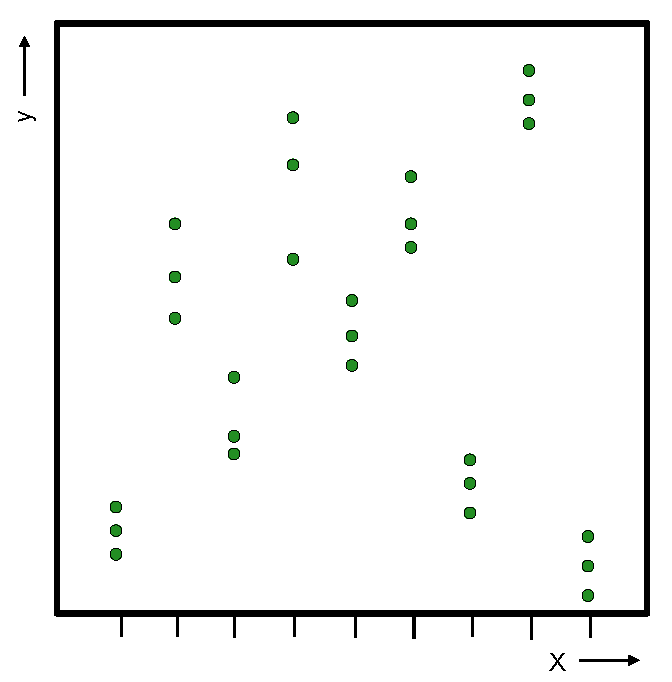
\includegraphics[width=0.75\textwidth]{Graphics/Intraclass}
\end{figure}

For nominally scaled data, neither \skalar{r_p} nor \skalar{r_s} is appropriate. However, we can use \skalar{r_i} \parencite{Har-13} to check wether certain values of \AbsVec{y} concentrate in certain classes of \AbsVec{x} (see fig. \ref{fig:Interclass}). If we have \skalar{A} groups with \skalar{B} data points per group, then \skalar{r_i} becomes:
\begin{align}
  r_i & = \frac{B}{B-1} \frac{A^{-1} \sum_{a=1}^A{(\bar{\AbsVec{y}}_a - \bar{\AbsVec{y}})^2}}{s^2} - \frac{1}{B - 1}  \\
      & \approx \frac{A^{-1} \sum_{a=1}^A{(\bar{\AbsVec{y}}_a - \bar{\AbsVec{y}})}}{s^2} \quad \mathrm{for\ large\ } B \\
  s^2 & = \frac{1}{AB} \sum_{b=1}^B{\sum_{a=1}^A{(\AbsVec{y}_{a,b} - \bar{\AbsVec{y}})^2}}
\end{align}
with \(\bar{\AbsVec{y}}_a \) the arithmetic mean of the \AbsVec{y}-values in the \skalar{a}-th group. Biggest limitation of \skalar{r_i} is that all groups need to have the same number of data points, \skalar{B}.

\subsection{\Name{Cramér}'s \skalar{V} for nominal/nominal association}

To compare two nominal scaled data vectors, each of length \skalar{n}, on uses a contingency table \arr{T} with \skalar{r} rows and \skalar{c} columns. Then \skalar{\chi^2} is calculated as follows:
\begin{align}
  \AbsVec{H}_i &= \sum_{j=1}^c{\frac{\arr{T}_{i,j}^2}{\AbsVec{C}_j}} \\
  A      &= \sum_{i=1}^r{\frac{\AbsVec{H}_i}{\skalar{r}_i}} \\
  \chi^2 &= (A-1) \times n \\
  f      &= (r-1) (c-1) \\
\end{align}
with \(\AbsVec{C}_j \) the column sums, \(\skalar{r}_i \) the row sums of the contingency table and \skalar{f} the degrees of freedom \parencite{Pea-00}. With \(\varphi^2 = \chi^2 / n \)
\begin{equation}
  V = \sqrt{\frac{\varphi^2}{\mathrm{min}(r-1, c-1)}}
\end{equation}
\skalar{V} reaches from \(0\ldots 1 \) (\emph{not} \(-1\ldots 1 \), with nominal values increase and decrease have no meaning!),  but tends to overestimate the strength of association between the data vectors. To correct for this bias, \skalar{\tilde{V}} is used:
\begin{align}
  \tilde{V} &= \sqrt{\frac{\tilde{\varphi}^2}{\mathrm{min}(\tilde{r}-1, \tilde{c}-1)}} \\
  \tilde{\varphi}^2 &= \mathrm{max}(0, \varphi^2 - \frac{(c-1)\times (r-1)}{(n-1)}) \\
  \tilde{c} &= c - \frac{(c-1)^2}{(n-1)} \\
  \tilde{r} &= r - \frac{(r-1)^2}{(n-1)}
\end{align}
To test for significance (\( H_0 \): no association between variables) one uses the \( \chi^2 \)-test with \skalar{f} degrees of freedom. \skalar{V} does not have a PRE interpretation.

\begin{lstlisting}[caption=Common correlation measures without PRE-interpretation for enumeration types]
  FUNCTION Chi2(const Contingency: ContTable;
    var Significance: SignificanceType): float;

  VAR
    H: array[0..MaxSteps] of float;
    i, j: word;
    A: float;

  BEGIN
    FOR i := 1 TO MaxSteps DO
      H[i] := 0.0;
    FOR i := 0 TO Contingency^.r DO
      FOR j := 0 TO Contingency^.c DO
        BEGIN
          A := Contingency^.Table[i, j];
          IF Contingency^.ColumnSums[j] = 0
            THEN A := 0
            ELSE A := A * A / Contingency^.ColumnSums[j];
          H[i] := H[i] + A;
        END;
    A := 0;
    FOR i := 0 TO Contingency^.r DO  // calculate first phi^2 = chi^2 / n
      BEGIN
        IF (Contingency^.RowSums[i] = 0)
          THEN
          ELSE A := A + H[i] / Contingency^.RowSums[i];
      END;
    A := (A - 1) * Contingency^.n;
    Significance.TestValue := A;
    Significance.Freedom := pred(Contingency^.r) * pred(Contingency^.c);
    Significance.P0 := IntegralChi(Significance.TestValue, round(Significance.Freedom));
    Result := A;
  END;


  FUNCTION Phi2(CONST Contingency: ContTable;
    VAR Significance: SignificanceType): float;

  VAR
    x: float;

  BEGIN
    x := chi2(Contingency, Significance);
    Result := x / Contingency^.n;
  END;

  FUNCTION CramersVTilde(chi2: float; r, c, n: word): float;

  VAR
    phi2, hilfs, ct, rt: float;

  BEGIN
    phi2 := chi2 / n;
    hilfs := phi2 - pred(c) * pred(r) / pred(n);     // now calculate tilde-version
    IF hilfs > 0
      THEN phi2 := hilfs
      ELSE phi2 := 0;
    ct := c - PRED(c) * PRED(c) / PRED(n);
    rt := r - PRED(r) * PRED(r) / PRED(n);
    IF rt > ct
      THEN rt := ct;                        // determine min(r~,c~)
    Result := sqrt(phi2 / (rt - 1));
  end;
\end{lstlisting}

\subsection{\Name{Guttman}'s coefficient of relative predictability \(\lambda \) for nominal/nominal association}

A different approach to measuring association is to attempt to predict the values of one variable in two different ways \parencite{Gut-41,Gin-06,Goo-54}. First, the values for one variable are predicted without knowing the values of a second variable. Then the values of the first variable are predicted again, after taking into account the values of the second variable. The extent to which the error of prediction for values of one variable can be reduced by knowing the value of a second variable forms the basis for the reduction in error approach to measuring association.

If the variables are cross-tabulated as described for \Name{Cramér}'s \skalar{V} above, then without knowledge of the columns one would pick that row \skalar{i} with the largest row-sum \(\skalar{r}_i \), as this prediction would minimise prediction error, which is \(E_n = n - \skalar{r}_i \).

If, however, it is known that the same individual is in column \skalar{j}, then one would pick the \skalar{i} such that \(\arr{T}_{i,j} \) is maximal, and the prediction error would become \(\AbsVec{C}_j - \arr{T}_{i,j} \). The total prediction error \skalar{E_j} is obtained by summing up the errors thus obtained for all rows.

\skalar{\lambda} is defined as the proportional reduction in error (PRE), that is
\begin{equation}
  \lambda = \frac{E_n - E_j}{E_n}
\end{equation}
and is the fraction by which the prediction error for the dependent variable can be reduced by knowledge of independent. For example, \(\lambda = 0.63 \) means that the error can be reduced by \SI{63}{\%} or about 2/3. Therefore, \(0 \leq \lambda \leq 1 \), with \(\lambda = 0 \) meaning no association, \(\lambda = 1 \) meaning perfect association. Thus:
\begin{align}
  EC_j &= \AbsVec{C}_j - \mathrm{max}(\arr{T}_{\cdot,j}) \\
  EC   &= \sum_{j=1}^c{EC_j} \\
  ET_r &= n - \mathrm{max}_i(\skalar{r}) \\
  \lambda_r &= \frac{ET_r - E_c}{ET_r} = \frac{n - \mathrm{max}_i(\skalar{r}) - \sum_{j=1}^r{(\AbsVec{C}_j -\mathrm{max}(\arr{T}_{\cdot,j}))}}{n - \mathrm{max}_i(\skalar{r})}
\end{align}
and analogous for \skalar{\lambda_c}:
\begin{align}
  ER_i &= \skalar{r}_i - \mathrm{max}(\arr{T}_{i,\cdot}) \\
  ER   &= \sum_{i=1}^c{EC_i} \\
  ET_c &= n - \mathrm{max}_j(\AbsVec{C}) \\
  \lambda_c &= \frac{ET_c - ER}{ET_c} = \frac{n - \mathrm{max}_j(\AbsVec{C}) - \sum_{i=1}^c{(\skalar{r}_i -\mathrm{max}(\arr{T}_{i,\cdot}))}}{n - \mathrm{max}_j(\AbsVec{C})}
\end{align}
Note that \skalar{\lambda_r} and \skalar{\lambda_c} are usually not identical. \parencite{Goo-54} gives a formula to calculate a symmetrical version of \skalar{\lambda}:
\begin{equation}
  \lambda = \frac{\sum_{i=1}^r{\mathrm{max}(\arr{T}_{i,\cdot})} + \sum_{j=1}^c{\mathrm{max}(\arr{T}_{\cdot,j})} - \mathrm{max}_i(\skalar{r}) - \mathrm{max}_j(\AbsVec{C})}{2n - [\mathrm{max}_i(\skalar{r}) + \mathrm{max}_j(\AbsVec{C})]}
\end{equation}
An almost identical result is obtained by calculating the average of \skalar{\lambda_r} and \skalar{\lambda_c} by eqn. \ref{eqn:AvCorr}.

\begin{table}
  \caption{Example data from \parencite{Goo-54}: Hair colour \Foreign{vs}. eye color. The results for various measures of association are given at the bottom. }
  \label{}
  \centering
    \begin{tabular}{c|cccc|c}
      \toprule
      Eye \(\backslash \) Hair & Fair & Brown & Black & Red  & \skalar{r} \\
      \midrule
      Blue       & 1768 &  807  &  189  &   47 & 2811       \\
      Grey/Green &  946 & 1387  &  746  &   53 & 3132       \\
      Brown      &  115 &  438  &  288  &   16 &  857       \\
      \midrule
      \AbsVec{C} & 2829 & 2632  & 1223  &  116 & n = 6800   \\
      \bottomrule
    \end{tabular}\\
    \vspace{2ex}

    \begin{tabular}{lllll}
 \(\lambda_r \) & \(\lambda_c \) & \(\lambda \) & \(\phi^2 \) & \(V \)    \\
      \midrule
      0.2241      & 0.1924      & 0.2076    & 0.1581   & 0.2812 \\
    \end{tabular}
\end{table}

\begin{lstlisting}[caption=\Name{Guttman}'s asymmetrical and symmetrical \skalar{\lambda}]
  FUNCTION lambda(CONST Contingency: ContTable): float;

  VAR
    i, j: word;
    MaxR, MaxC, SumMaxTi, SumMaxTj: float;
    MaxTi, MaxTj: ARRAY[0..MaxSteps] OF WORD;
    // can't be vectorType AS 0 must be legal index

  BEGIN
    FOR i := 0 TO MaxSteps DO
      BEGIN
        MaxTi[i] := 0;
        MaxTj[i] := 0;
      END;
    SumMaxTi := 0;
    FOR i := 0 TO Contingency^.r DO
      BEGIN
        FOR j := 0 TO Contingency^.c DO
          IF MaxTi[i] < Contingency^.Table[i, j] THEN
            MaxTi[i] := Contingency^.Table[i, j];
        SumMaxTi := SumMaxTi + MaxTi[i];
      END;
    SumMaxTj := 0;
    FOR j := 0 TO Contingency^.c DO
      BEGIN
        FOR i := 0 TO Contingency^.r DO
          IF MaxTj[j] < Contingency^.Table[i, j]
            THEN MaxTj[j] := Contingency^.Table[i, j];
        SumMaxTj := SumMaxTj + MaxTj[j];
      END;
    MaxR := Contingency^.RowSums[0];
    FOR i := 1 TO Contingency^.r DO
      IF (Contingency^.RowSums[i] > MaxR)
        THEN MaxR := Contingency^.RowSums[i];
    MaxC := Contingency^.ColumnSums[0];
    FOR j := 1 TO Contingency^.c DO
      IF (Contingency^.ColumnSums[j] > MaxC)
        THEN MaxC := Contingency^.ColumnSums[j];
    Result := (2 * Contingency^.n - (MaxR + MaxC));
    IF Result = 0
      THEN           // ???
      ELSE lambda := (SumMaxTi + SumMaxTj - MaxR - MaxC) / lambda;
  END;


  FUNCTION lambda_r(CONST Contingency: ContTable): float;

  VAR
    i, j: WORD;
    MaxR, MaxT, SumCT: float;

  BEGIN
    MaxR := 0;
    FOR i := 0 TO Contingency^.r DO
      IF (Contingency^.RowSums[i] > MaxR)
        THEN MaxR := Contingency^.RowSums[i];
    SumCT := 0;
    FOR j := 0 TO Contingency^.c DO
      BEGIN
        MaxT := Contingency^.Table[0, j];
        FOR i := 1 TO Contingency^.r DO
          IF (MaxT < Contingency^.Table[i, j])
            THEN MaxT := Contingency^.Table[i, j];
        SumCT := SumCT + Contingency^.ColumnSums[j] - MaxT;
      END;
    Result := Contingency^.n - MaxR;
    IF (Result = 0)
      THEN          // ???
      ELSE lambda_r := (Contingency^.n - MaxR - SumCT) / lambda_r;
  END;


  FUNCTION lambda_c(CONST Contingency: ContTable): float;

  VAR
    i, j: WORD;
    MaxC, MaxT, SumRT: float;

  BEGIN
    MaxC := 0;
    FOR j := 0 TO Contingency^.c DO
      IF (Contingency^.ColumnSums[j] > MaxC)
        THEN MaxC := Contingency^.ColumnSums[j];
    SumRT := 0;
    FOR i := 0 TO Contingency^.r DO
      BEGIN
        MaxT := Contingency^.Table[i, 0];
        FOR j := 1 TO Contingency^.c DO
          IF (MaxT < Contingency^.Table[i, j])
            THEN MaxT := Contingency^.Table[i, j];
        SumRT := SumRT + Contingency^.RowSums[i] - MaxT;
      END;
    lambda_c := (Contingency^.n - MaxC);
    IF lambda_c = 0
      THEN          // ???
      ELSE lambda_c := (Contingency^.n - MaxC - SumRT) / lambda_c;
  END;
\end{lstlisting}


\subsection{\Name{Freeman}'s measure of association \skalar{\theta} for nominal/ordinal association}

\skalar{\theta}\ measures the reduction of error if an ordinal dependent variable is predicted from an independent variable on the nominal scale, compared to random guessing \parencite{Fre-65,Fre-76}. It is therefore a PRE measure of association. Because variables on the nominal scale are unordered \skalar{\theta} can have only positive values, ranging from \(0\ldots 1 \):
\begin{equation}
  \theta = \frac{\sum_{i=1}^{r}{D_i}}{T}
\end{equation}
with \(D_i = |f_b - f_a| \) for each comparison the difference of frequencies below and above, and \skalar{T} the number of comparisons made. Ties are considered to arise from our inability to precisely rank people and should be split between orders, however, \(|(f_b - 1/2 f_\mathrm{ties}) - (f_a - 1/2 f_\mathrm{ties}) = |f_b - f_a| \), so ties are ignored. \parencite{Fre-65} gives as example social adjustment (ranked, \Foreign{i.e.}, ordinal) \Foreign{vs.} marital status (nominal):

\begin{tabular}{l|rrrrr|r}
  \toprule
  Status \( \backslash \) Rank & 5  & 4  & 3  & 2  & 1  & \(\arr{S} \) \\
  \midrule
  Single   &  1 &  2 &  5 &  2 &  0 & 10 \\
  Married  & 10 &  5 &  5 &  0 &  0 & 20 \\
  Widowed  &  0 &  0 &  2 &  2 &  1 &  5 \\
  Divorced &  0 &  0 &  0 &  2 &  3 &  5 \\
  \bottomrule
\end{tabular}

For the comparison of single and married persons, we get:

\begin{tabular}{r|rrrrr}
  \toprule
  Rank & \(n_r \)  & \(n_b \)  & \(\Pi_b \) & \(n_a \)  & \(\Pi_a \) \\
  \midrule
  5    &     1  &   10   &   10    &    0   &      0  \\
  4    &     2  &    5   &   10    &   10   &     20  \\
  3    &     5  &    0   &    0    &   15   &     75  \\
  2    &     2  &    0   &    0    &   20   &     40  \\
  1    &     0  &    0   &    0    &   18   &      0  \\
  \midrule
 \(f \)  &        &        &   20    &        &    135  \\
  \bottomrule
\end{tabular}

and \(\skalar{D_i} = |f_b - f_a| = |20 - 135| = 115 \). For single and widowed persons, we get:

\begin{tabular}{r|rrrrr}
  \toprule
  Rank & \(n_r \)  & \(n_b \)  & \(\Pi_b \) & \(n_a \)  & \(\Pi_a \) \\
  \midrule
  5    &     1  &    5   &    5    &    0   &      0  \\
  4    &     2  &    5   &   10    &    0   &      0  \\
  3    &     5  &    3   &   15    &    0   &      0  \\
  2    &     2  &    1   &    2    &    2   &      4  \\
  1    &     0  &    0   &    0    &    4   &      0  \\
  \midrule
 \(f \)  &        &        &   32    &        &      4  \\
  \bottomrule
\end{tabular}

and \(\skalar{D_i} = |f_b - f_a| = |32 - 4| = 28 \).  Analogously for the other comparisons:

\begin{tabular}{llrrr}
  \toprule
  Status 1 & Status 2 & \(f_b \) & \(f_a \) & \(D_i \) \\
  \midrule
  single   & divorced &  46   & 0 &  46 \\
  married  & widowed  &  90   & 0 &  90 \\
  married  & divorced & 100   & 0 & 100 \\
  widowed  & divorced &  16   & 2 &  14 \\
  \bottomrule
\end{tabular}

Thus, \(\sum{D_i} = 115 + 28 + 46 + 90 + 100 + 14 = 393 \). \skalar{T} is calculated from the row sums of the data table:
\begin{equation}
  T = 10*20 + 10*5 + 10*5 + 20*5 + 20*5 + 5*5 = 525
\end{equation}
Then \(\theta = 393/525 = 0.75 \)

\subsubsection{Significance of \(\theta \)}

The distribution of \(\theta \) is unknown. If the nominal vector has only two different values, the \Name{Wilcoxon-Mann-Whitney} U-test (first published in \parencite{Deu-14}) can be used.

\begin{lstlisting}[caption=\Name{Freeman}'s measure of association \skalar{\theta}]
  FUNCTION theta(CONST Contingency: ContTable): float;

  VAR
    i, j, k, l: word;
    SumT, fa, fb, SumDi, nr: float;

  BEGIN
    SumT := 0;
    FOR i := 0 TO Contingency^.r DO
      FOR j := succ(i) TO Contingency^.r DO
        SumT := SumT + Contingency^.RowSums[i] * Contingency^.RowSums[j];
    SumDi := 0;
    FOR i := 0 TO Contingency^.r DO
      BEGIN
        FOR k := succ(i) TO Contingency^.r DO
          BEGIN
            fa := 0;
            fb := 0;
            FOR j := 0 TO Contingency^.c DO
              BEGIN
                nr := Contingency^.Table[i, j];
                IF (j < Contingency^.c)
                  THEN
                    FOR l := succ(j) TO Contingency^.c DO
                      fa := fa + Contingency^.Table[k, l] * nr;
                IF (j > 0)
                  THEN // this check actually is necessary
                    FOR l := pred(j) DOWNTO 0 DO
                      fb := fb + Contingency^.Table[k, l] * nr;
              END;
            SumDi := SumDi + abs(fb - fa);
          END;
      END;
    IF (SumT = 0)
      THEN Result := 0    // ???
      ELSE Result := SumDi / SumT;
  END;
\end{lstlisting}


\subsection{\skalar{\eta^2} for nominal/cardinal association}

\skalar{\eta^2} is also a PRE measure \parencite{Ano-16}. Assume we have a vector \AbsVec{y} of cardinal (interval or rational) data. If we had to predict a \(\AbsVec{y}_i \), we would use the arithmetic mean \(\bar{\AbsVec{y}} \) and the prediction error becomes
\begin{equation}
  E_1 = \sum_{i=1}^n{(y_i - \bar{y})^2}
\end{equation}
If, however, we know that the test person \skalar{i} belongs into group \skalar{k} of some nominal scaled variable \AbsVec{x}, then the predicted value would be the group average \(\bar{y}_k \) and the prediction error becomes:
\begin{equation}
  E_2 = \sum_k{\sum_{i=1}^n{(y_i - \bar{y}_k)^2 \delta_{ik}}} \quad \mathrm{for}\quad \delta_{ik} = \left\{
                                                                           \begin{array}{rl}
                                                                              1 & \mathrm{if}\ i = k \\
                                                                              0 & \mathrm{else} \\
                                                                           \end{array}
                                                                          \right.
\end{equation}
Then \skalar{\eta^2} becomes:
\begin{equation}
  \eta^2 = \frac{E_1 - E_2}{E_1} = 1 - \frac{E_2}{E_1}= 1 - \frac{\sum_k{\sum_{i=1}^n{(y_i - \bar{y}_k)^2 \delta_{ik}}}}{\sum_{i=1}^n{(y_i - \bar{y})^2}}
\end{equation}
Thus \skalar{\eta^2} is the reduction in error of \(\AbsVec{y}_i \) by knowing \(\AbsVec{x}_i \). It goes from \(0\ldots 1 \) and is unidirectional because nominal data are unordered.

\subsubsection{Significance testing of \(\eta^2 \)}

The correlation is the greater the more different the means of the cardinal variable are in the different classes of the nominal. Thus the Null-hypothesis would be H\textsubscript{0} : All classes have indistinguishable means. \Name{Fisher}'s \skalar{F}-test can be used. It is based on the idea that the average of the sample variances \skalar{s^2_j} (\( j = 1..r \)) is a first estimate \skalar{\hat{s}_1^2} of the variance in the population \skalar{\sigma^2}. If all samples were taken from the same population, the variance \(s^2_{\bar Y} \) of the \skalar{r} means should give a second estimate \skalar{\hat{s}_2^2} of the population variance. \skalar{F} is the ratio between these estimates:
\begin{align}
  \hat{s}^2_1 &= \frac{\sum_{j=1}^r{s_j^2}}{r} \\
  s^2_{\bar Y} &= \frac{\sum_{j=1}^r{(\bar{\AbsVec{x}}_j - \bar{\AbsVec{x}})}}{r-1} \\
  \hat{s}^2_2 &= n_j s^2_{\bar Y}          \\
  F                &= \frac{\hat{s}_2^2}{\hat{s}_1^2} = \frac{\eta^2}{1-\eta^2} \times \frac{n - r}{r-1}\\
\end{align}
with \skalar{n_j} the size of the groups. The degree of freedom for the numerator is \(r-1 \), for the denominator \(n-r \), with \skalar{n} the total sample size. The second part of the equation for \skalar{F} can be used even if the group sizes are not equal.

If this ratio is near \num{1.0}, differences of group means probably represent sampling variation between samples taken from a single population. If \skalar{F} is large, this Null-hypothesis can be rejected, the samples probably come from different populations.

\begin{lstlisting}[caption=Nominal/Nominal association]
FUNCTION eta_sqr(CONST NominalVector, CardinalVector: VectorTyp;
  VAR Significance: SignificanceType): float;

VAR
  i, k, n, Classes, Length, Value1: WORD;
  E1, E2, total, r: float;
  SumOfK: array [0..MaxSteps] of float;
  NofK: ARRAY [0..MaxSteps] OF WORD;

BEGIN
  IF NOT (TestDataVectorLength(NominalVector, CardinalVector)) THEN EXIT;
  Length := VectorLength(NominalVector);
  Classes := 0;
  FOR i := 1 TO Length DO
    BEGIN
      IF IsNaN(GetVectorElement(NominalVector, i))
        THEN
        ELSE IF (round(GetVectorElement(NominalVector, i)) > Classes)
               THEN Classes := ROUND(GetVectorElement(NominalVector, i));
      // find largest value for nominal vector
    END;
  FOR i := 0 TO Classes DO
    BEGIN
      NofK[i] := 0;
      SumOfK[i] := 0;
    END;
  Total := 0;
  n := 0;
  FOR i := 1 TO Length DO
    IF ((IsNaN(GetVectorElement(NominalVector, i))) OR
      (IsNaN(GetVectorElement(CardinalVector, i))))
      THEN   // ignore NaNs
      ELSE
        BEGIN
          Value1 := trunc(GetVectorElement(NominalVector, i));
          Inc(NofK[Value1]);
          // how many x are there for any of the 0..Classes values of x?
          SumOfK[Value1] := SumOfK[Value1] + GetVectorElement(CardinalVector, i);
        END;
  FOR k := 0 TO Classes DO
    BEGIN
      n := n + NofK[k];                         // number of data pairs that are not NaN
      Total := Total + SumOfK[k];
      IF (NofK[k] <> 0)
        THEN SumOfK[k] := SumOfK[k] / NofK[k]; // group-averages
    END;
  Total := Total / n;                          // average over all data
  E1 := 0;
  E2 := 0;
  FOR i := 1 TO Length DO
    BEGIN
      IF ((IsNaN(GetVectorElement(NominalVector, i))) OR
        (IsNaN(GetVectorElement(CardinalVector, i))))
        THEN
        ELSE E1 := E1 + sqr(GetVectorElement(CardinalVector, i) - Total);
    END;
  FOR i := 1 TO Length DO
    BEGIN
      IF ((IsNaN(GetVectorElement(NominalVector, i))) OR
          (IsNaN(GetVectorElement(CardinalVector, i))))
        THEN
        ELSE E2 := E2 + sqr(GetVectorElement(CardinalVector, i) -
                   SumOfK[trunc(GetVectorElement(NominalVector, i))]);
    END;
  IF (E1 = 0)
    THEN r := 0.0    // ???
    ELSE r := 1 - E2 / E1;
  IF (r = 1)
    THEN
      BEGIN
        Significance.P0 := NaN;
        Significance.Freedom := n - r;
        Significance.TestValue := NaN;
      END
    ELSE
      BEGIN
        Significance.TestValue := r / (1 - r) * (n - r) / (r - 1);
        // calculate F
        Significance.Freedom := n - r;
        // other is r-1 and can be calculated in calling program
        Significance.P0 := Integral_F(Significance.TestValue, round(n - r), round(r - 1));
        // calculate probability for 0-hypotheses
        Result := r;
      END;
END;
\end{lstlisting}

\subsection{Latent correlation}

Sometimes variables on an ordinal scale can be thought of as quantised representation of an interval-scaled, unobserved (latent) variable. In these cases the \textbf{tetrachoric} correlation (for binary variables) or the \textbf{polychoric} correlation coefficients can be used. These names refer to series expansions that were used before the availability of computers to calculate the correlation coefficient, this calculation method is obsolete so the term "latent" correlation is now preferred \parencite{Ueb-15,Ols-79}. Note that according to \parencite{Hub-82} the tetrachoric correlation coefficient (his \skalar{A_{30}}) has undesirable statistical properties and should be replaced by \Name{McConnaughey}'s correlation.

For example, latent correlation is used to measure rater agreement (correlation of results if ratings were made on a interval rather than on a \Name{Likert} \parencite{Lik-32} scale). The method can be used even to compare studies with different rating levels or raters who use different rating levels. Example: A disease may be diagnosed if a trait (a cardinal variable) exceeds a certain threshold, resulting in a dichotomous scale (disease present/absent). From the contingency table of the diagnostic results of two raters one can estimate the threshold of both raters (\skalar{t_1, t_2}) and the radius of the ellipse that would form if both raters used a cardinal scale and their measurements were plotted against each other (\skalar{\rho} or tetrachoric correlation coefficient \skalar{r_*}). The polychoric case is an extension of this concept to multiple rating levels, that is, multiple thresholds and more cells in the contingency table.

If a patient comes to the raters with a true latent trait level \skalar{t}, the raters will get the
impression of latent trait level \skalar{y_1 ,y_2}, leading to the manifest rating \skalar{x_1, x_2}. Then the
model is:
\begin{align}
  y_1 &= b_1 t + \varepsilon_1 \\
  y_2 &= b_2 t + \varepsilon_2
\end{align}
with \skalar{b_1, b_2} regression coefficients and \skalar{\varepsilon_1, \varepsilon_2} error terms. If both \skalar{t} and the errors are normally distributed and independent between raters and cases, then \skalar{y_1, y_2} must also be normally distributed and \(b_1 = b_2 = b \). We define \(r_* \equiv b^2 \). It is possible to extend this model to skewed latent traits or for more than two raters. The R-packages \texttt{polycor} and \texttt{psych} can calculate latent correlations.



\printbibliography[heading=subbibliography]
\end{refsection}

  % -*- TeX:UK -*-
\chapter{Linear and linearising Regression}
\begin{refsection}

\abstract{In many cases, a dependent variable \AbsVec{y} can be described as linear function of an independent (predictor) variable \AbsVec{x}, using the criterion of minimal sum of squared residuals. Some important non-linear functions can be linearised by a suitable transformation of \AbsVec{x, y}; even if this results in biased estimates for the parameters. Non-parametric methods should be used for regression if the conditions of normality, uncorrelatedness and homoscedasticity of the error are violated.  }

The interface for the unit is
\begin{lstlisting}[caption=Interface]
  UNIT LinearRegression;

  INTERFACE

  USES math, MathFunc, Vector, Stat, Correlations;

  CONST RegressionError : BOOLEAN = FALSE;

  TYPE CurveTyp  = (Origin, Linear, Exponential, Power, Hyperbola, Inverse, Maximum,
                    Sigmoidal, ExpSigmoidal, ModPower, Hill);
       ResultTyp = RECORD
                     a, sa,                            // intercept
                     b, sb,                            // slope
                     m, sm,                            // exponent
                     r, t, P0 : double;                // TEST statistics
                   END;

  PROCEDURE Approximation(CONST x, y, weight : VectorTyp; ct : CurveTyp;
            VAR yCalc : VectorTyp; VAR Res : ResultTyp);
  // linear regression for least sum of squares

  PROCEDURE Transformation(CONST xOrig, yOrig : VectorTyp; VAR xTrans, yTrans : VectorTyp;
                           ct : CurveTyp; Schaetzwert : double);
  // transformation of x, y TO linearise

  PROCEDURE Retransform (CONST x, yTrans : Vectortyp; VAR TRes, Res : ResultTyp;
                         ct : CurveTyp; Schaetzwert : double;
                         VAR yCalc : VectorTyp);
  // re-transformation of linear results to curve

  PROCEDURE LinFit (Data : MatrixTyp;  mwt: BOOLEAN; VAR a, b, siga, sigb, chi2, q: real);
  { Robuste Daten-Modellierung nach Press et al.: Numerical Recepies in Pascal,
    Cambridge 1989, pp 590-8
    Anpassung von Daten an eine Ausgleichsgerade. Dabei wird jedoch die uebliche
    Annahme fallengelassen, alle Datenpunkte haetten die gleiche Standardabweichung.
    Eingabe: Data enthaelt die Daten, dabei stehen in jeder Zeile x, y und die
             Standardabweichung fuer y (falls letztere nicht zur Verfuegung
             stehen, muá mwt = false gesetzt werden).
    Ausgabe: a und b sind die Parameter des Modells, siga und sigb die Fehler-
             grenzen. chi2 ist ein Mass fuer die Guete des Modells, q die War-
             scheinlichkeit gegen dieses Modell. }

  PROCEDURE Deming (CONST x, y : VectorTyp; delta : double;
                    VAR xCalc, yCalc : VectorTyp; VAR Res : ResultTyp);
  // Deming regression for data with errors in x and y

  PROCEDURE TheilSenKendall (CONST x, y : VectorTyp; VAR yCalc : VectorTyp;
                             VAR Res : ResultTyp);
  // non-parametric regression

  PROCEDURE Eisenthal (CONST Substrate, Velocity : VectorTyp; VAR yCalc : VectorTyp;
                             VAR Res : ResultTyp);
  // Eisenthal & Cornish-Bowden 1974



  IMPLEMENTATION
\end{lstlisting}



\section{Linear regression}

For further information, consult \parencite{Noa-80,Spa-82,Wil-61,Abr-64}. Given a pair of vectors \AbsVec{x, y}, with \AbsVec{x} the independent (controlled, predictor) and \AbsVec{y} the dependent (predicted) variable, it is possible to calculate a line \(\hat{\AbsVec{y}} = f(\AbsVec{x}) = a + b \AbsVec{x} + \epsilon \) through these data pairs so that the sum of squared residuals \(\sum_{i=1}^{n}{(\AbsVec{y}_i - \hat{\AbsVec{y}}_i)^2} \) becomes minimal. Note that this is possible even when the data are not well represented by the model, in that case the fit will be poor, the squared residuals will be large and a plot of the residuals as function of \AbsVec{x} (or \(\hat{\AbsVec{y}} \)) will show a non-random pattern.

\begin{rules}
  Hence it is of utmost importance to \emph{always} plot both \(\AbsVec{y}_i \) and \(\hat{\AbsVec{y}}_i - \AbsVec{y}_i \) as function of \(\AbsVec{x}_i \) and to visually check these plots for unexpected patterns.
\end{rules}

The most common case of linear regression is data that are on a straight line, however, we speak of linear regression whenever the second and higher derivatives of the fitting function with respect to the parameters are all zero \parencite{Joh-10}.  Then the Gauss-Newton algorithm will require only a single iteration for any initial ‘‘guesses’’ of the fitting parameter values, which therefore can all be set to zero.

\subsection{Requirements for linear regression}

The data \AbsVec{x, y} should meet a couple of requirements:
\begin{itemize}
  \item{All error is in the \AbsVec{y}-vector, the \AbsVec{x}-vector is error-free. If both dependent and independent variables have errors, one can try a \Name{Deming} regression \parencite{Dem-43}.}
  \item{The error terms \(\epsilon \) should be \textbf{uncorrelated}, that is, knowledge of \(\epsilon_i \) should not allow the prediction of \(\epsilon_{i+1} \). For example, time series data are prone to correlations of error terms, because drift affects data the more similarly, the closer they are in time. A plot of \(\hat{\AbsVec{y}}_i - \AbsVec{y}_i \) as function of time can reveal this, perhaps followed by a runs test. Correlation of error may also occur if some data points have factors in common that the study doesn't test for. For example, in a study of height vs weight of persons, such correlations can arise if some test subjects were raised under the same environmental influences (say, in siblings), or if repeat measurements were made on the same subject. In effect, such correlations reduce the confidence intervals of parameters, making the data appear more precise than they actually are.}
  \item{The error should be \textbf{normally distributed}.}
  \item{\textbf{Homoscedasticity} of the data means that \(\AbsVec{y}_i - \hat{\AbsVec{y}}_i\) is independent of \AbsVec{x}. Depending on experimental design, especially for \AbsVec{y}-values spanning several orders of magnitude, \(\hat{\AbsVec{y}}_i - \AbsVec{y}_i \) may increase with \AbsVec{x}, so that the relative error stays constant. In a plot of residuals, one would see a funnel. Linear regression of such data by the least-squares criterion leads to biased parameters with underestimated standard deviations. A better approach would be a fit by minimal \(\chi^2 \), for example by the simplex algorithm (see chapter \ref{chap:Simplex} on page \pageref{chap:Simplex}). Alternatively, one can perform a weighted linear regression. }
  \item{The data should be free of \textbf{outliers}, that is, data points with extremely large residuals. Such data are obvious in a plot of the residuals. Even better is to plot the \emph{studentised residuals}, that is the residuals divided by their estimated standard error. Any data point with a studentised residual larger than \num{3} is suspect. If the outlier is the result of a measurement error, it should be removed. However, outliers may the result of an incomplete model (variables that affect the result, but were not accounted for). Robust (non-parametric) fitting methods, for example the \Name{Theil–Sen-Kendall}-estimator \parencite{The-50}, can be used if there are many outliers.  }
  \item{The distribution of data with respect to \AbsVec{x} should be reasonably even. Single data points with very extreme \AbsVec{x}-values may have a strong influence on the regression line, they have \textbf{high leverage}. Any problems with such data points will unduely affect the data fit. The leverage statistics for the \skalar{i}-th data point \(\AbsVec{h}_i = \frac{(\AbsVec{x}_i - \bar{\AbsVec{x}})^2}{\sum(\AbsVec{x} - \bar{\AbsVec{x}})^2} \) is a number \(0 \leq \AbsVec{h}_i \leq 1 \), and \(\bar{\AbsVec{h}} = \frac{p}{n} \). Thus any observation where \(\AbsVec{h}_i \gg \bar{\AbsVec{h}} \) is suspect. In multiple regression, \(\AbsVec{h} = \diag(\arr{H}) = \diag(\arr{X}(\arr{X}^T\arr{X})^{-1}\arr{X}^T) \) the diagonal of the hat-matrix.   }
\end{itemize}

\subsection{Algorithm}

\subsubsection{Parameters}

In matrix terms, the position of the minimum of the \acs{RSS} is given by \( \hat{\beta} = (\arr{X}^T \arr{X})^{-1} \arr{X}^T\AbsVec{y} \), its value by \( \mathrm{RSS}(\hat{\beta}) = \AbsVec{y}^T\AbsVec{y} - \hat{\beta}^T \arr{X}^T \arr{X} \hat{\beta} \) and the \acs{RSS} in the vicinity of the minimum by \( \mathrm{RSS}(\beta) = \mathrm{RSS}(\hat{\beta}) + (\beta - \hat{\beta})^T \arr{X}^T\arr{X}(\beta - \hat{\beta}) \) \parencite{Joh-10b}.

For a two-variable regression \( \hat{\AbsVec{y}}_i = a + b\AbsVec{x}_i \), the calculation is performed as follows:  With \(S_\AbsVec{x} = \sum_{i=1}^n{\AbsVec{x}_i} \), \(S_\AbsVec{y} = \sum_{i=1}^n{\AbsVec{y}_i} \), \(S_\AbsVec{xx} = \sum_{i=1}^n{(\AbsVec{x}_i^2)} \), \(S_\AbsVec{yy} = \sum_{i=1}^n{(\AbsVec{y}_i^2)} \), \(S_\AbsVec{xy} = \sum_{i=1}^n{(\AbsVec{x}_i\AbsVec{y}_i)} \), the estimated slope of the regression line \(b = \hat{\beta}_1 \) is
\begin{equation}
  b = \frac{n S_\AbsVec{xy} - S_\AbsVec{x}S_\AbsVec{y}}{n S_\AbsVec{xx} - S_\AbsVec{x}^2}
    = \frac{\mathrm{Cov}_{\AbsVec{x,y}}}{\mathrm{Var}_\AbsVec{x}}
\end{equation}
and the intercept \(a = \hat{\beta}_0 \)
\begin{equation}
  a = \bar{\AbsVec{y}} - b\bar{\AbsVec{x}}
\end{equation}
In other words, the regression line goes through the centroid of the data \((\bar{\AbsVec{x}}, \bar{\AbsVec{y}}) \) and is rotated until the sum of squared residuals is minimal.

A line can be forced through the origin, that is, \(a = 0 \). Then
\begin{equation}
  b = \frac{S_\AbsVec{xy}}{S_\AbsVec{xx}}
\end{equation}
Instead of (0,0), the line can go through any point (\skalar{h,k}):
\begin{equation}
  b = \frac{\overline{(\AbsVec{x} - h) (\AbsVec{y} - k)}}{\overline{(\AbsVec{x}-h)^2}}
    = \frac{\mathrm{Cov}_\AbsVec{x,y} + (\bar{\AbsVec{x}} - h) (\bar{\AbsVec{y}} - k)}{\mathrm{Var}_\AbsVec{x} + (\bar{\AbsVec{x}} - h)^2}
\end{equation}

\subsubsection{Correlation coefficient}

\Name{Pearson}'s product moment correlation between \AbsVec{x} and \AbsVec{y} is
\begin{equation}
 r = \frac{n S_\AbsVec{xy} - S_\AbsVec{x}S_\AbsVec{y}}{\sqrt{(n S_\AbsVec{xx} - S_\AbsVec{x}^2)(nS_\AbsVec{yy} - S_\AbsVec{y}^2)}}
\end{equation}
The square of \skalar{r} is the \textbf{coefficient of determination} \skalar{r^2}, the fraction of variance in the \AbsVec{y}-data that is explained by \AbsVec{x}. If the  \AbsVec{y}-data were predicted without knowledge of \AbsVec{x}, then one would use \(\bar{\AbsVec{y}} \) as best predictor, and the total error would be \(E_1 = \sum_{i=1}^n{(\AbsVec{y}_i - \bar{\AbsVec{y}})^2} \), the \textbf{\acf{TSS}}. If \AbsVec{x} is used for prediction, the new total error becomes \(E_2 = \sum_{i=1}^n{(\AbsVec{y}_i - \hat{\AbsVec{y}}_i)^2} \), the \textbf{\acf{RSS}}. Then \(r^2 = \frac{E_1 - E_2}{E_1} = 1 - \frac{E_2}{E_1} \), the \textbf{\acf{PRE}} from knowledge of \AbsVec{x} \parencite{Fre-65}. The \textbf{\acf{ESS}} \( = \sum_{i=1}^n{(\hat{\AbsVec{y}}_i - \bar{\AbsVec{y}})^2} = \mathrm{TSS} - \mathrm{RSS} \).

\begin{figure}
 \caption{\emph{Top}: Regression analysis for synthetic data (\num{100} data points, \(y = 1 + 2x \) with random noise added). The regression of \AbsVec{y} from \AbsVec{x} yields a different line from the regression of \AbsVec{x} from \AbsVec{y}. Both lines go through \((\bar{\AbsVec{x}}, \bar{\AbsVec{y}}) \), their angle \(\alpha \) is proportional to the correlation coefficient \skalar{r}. Note that the noise affects the estimate for the intercept much more than that for the slope. \emph{Bottom}: The residuals are randomly distributed around their average and show no discernible pattern. }
 \label{fig:CorReg}
 \centering
 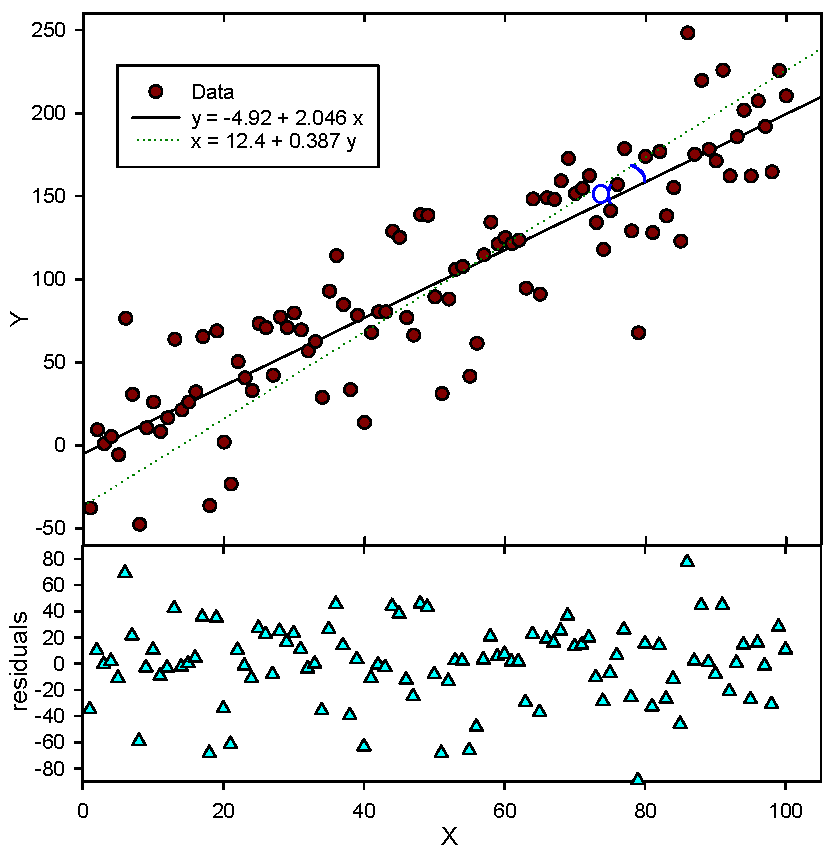
\includegraphics[width=0.75\textwidth]{Graphics/Correlation-Error}
\end{figure}

If one calculates the regression line between \AbsVec{x} and \AbsVec{y} with the parameters \(a_x, b_x \) and the regression line between \AbsVec{y} and \AbsVec{x} with the parameters \(a_y, b_y \) (see fig. \ref{fig:CorReg}), then these lines form an angle \(\alpha \) -- recall that both lines intersect at \((\bar{\AbsVec{x}}, \bar{\AbsVec{y}}) \). This angle is proportional to \skalar{r}, it is \ang{0} for \(r = 1 \) and \ang{90} for \(r = 0 \). The correlation coefficient is \(r = \sqrt{b_x b_y} \).

Yet another alternative interpretation of \skalar{r} is the slope of the regression line through the \skalar{z}-standardised data points. This line passes through the origin, because the arithmetic mean of \skalar{z}-standardised data is zero.

It is possible to test the regression for significance, that is, to test the 0-hypothesis \(H_0 : r = 0 \) against the alternative hypothesis \(H_1 : r \neq 0 \). For this, a \skalar{t}-value is calculated according to eqn. \ref{eqn:rt-sig}, then the degrees of freedom \(\nu = n - q \) is the number of measured values \skalar{n} minus the number of parameters used \skalar{q}.

In simple regression, \(R^2 = r^2 \), but in multiple regression, \(R^2 = \mathrm{Cor}(\AbsVec{y},\hat{\AbsVec{y}}) \neq r^2 \). The algorithm then maximises \(R^2 \).

It is sometimes necessary to decide between different models, with different number of parameters \(p \). Because
\begin{equation}
  R^2 = 1 - \frac{\sum{(\AbsVec{y}_i - \hat{\AbsVec{y}}_i)^2}}{\sum{(\AbsVec{y}_i - \bar{\AbsVec{y}})^2}}
\end{equation}
, \(R^2 \) will always increase with \(p \). This results from a reduction in training error, which may not correspond to a reduction in test error (overfitting). Thus, to compare models with different \(p \), we use the \textbf{adjusted \(R^2 \)}
\begin{equation}
  R^2_a = 1 - \frac{\sum{(\AbsVec{y}_i - \hat{\AbsVec{y}}_i)^2} / (n-p-1)}{\sum{(\AbsVec{y}_i - \bar{\AbsVec{y}})^2} / (n-1)}
\end{equation}
which may increase or decrease as additional parameters are added. Irrelevant parameters will decrease the sum of squared residuals only marginally, this is over-compensated by the increase of \(p \) in the denominator.
Other values used to identify the best number of parameters are
\begin{align}
  C_p          &= \frac{1}{n} \left(\sum_{i=1}^n{(\AbsVec{y}_i - \hat{\AbsVec{y}}_i)^2} + 2p\hat{\sigma}^2\right) \\
  \mathrm{AIC} &= \frac{1}{n\hat{\sigma}^2} \left(\sum_{i=1}^n{(\AbsVec{y}_i - \hat{\AbsVec{y}}_i)^2} + 2p\hat{\sigma}^2\right) \\
  \mathrm{BIC} &= \frac{1}{n} \left(\sum_{i=1}^n{(\AbsVec{y}_i - \hat{\AbsVec{y}}_i)^2} + \log(n)p\hat{\sigma}^2\right)
\end{align}
, which are closely related to each other. Whilst we are looking for a maximum of \(R^2 \), we look for the minimum of \(C_p \), \acs{BIC} and \acs{AIC}.

\subsubsection{Error estimates for the parameters \skalar{a, b}}

The variance of the residuals is
\begin{equation}
   s_\epsilon^2 = \frac{1}{n (n-2)} [n S_\AbsVec{yy} - S_\AbsVec{y}^2 - b^2 (n S_\AbsVec{xx} - S_\AbsVec{x}^2)]
\end{equation}
, the variance of \skalar{b}
\begin{equation}
  s_b^2 = \frac{n s_\epsilon^2}{n S_\AbsVec{xx} - S_\AbsVec{x}^2}
\end{equation}
and the variance of \skalar{a}
\begin{equation}
  s_a^2 = \frac{1}{n} s_b^2 S_\AbsVec{xx}
\end{equation}

The degrees of freedom is \(\nu = n - q \) with \skalar{q} the number of parameters  estimated, here 2. Given the 0.975-quantile of the \skalar{t}-distribution with \(\nu \) degrees of freedom \(t^*_\nu \), we can calculate the \SI{97.5}{\%} confidence intervals for the parameters to
\begin{equation}
  a \pm t^*_\nu \sqrt{s_a^2}\qquad  b \pm t^*_\nu \sqrt{s_b^2}
\end{equation}

\subsubsection{Tests for \(H_0: r=0 \), \(H_0: b=b_0 \) and \(H_0: a=a_0 \)  }

It is sometimes necessary to decide, whether there actually is a significant relationship between the dependent and independent variable, that is, we test \(H_0: r = 0 \) against \(H_1: r \neq 0 \). For this we can either do an \skalar{F}-test:
\begin{eqnarray}
  \nonumber
  F &=& \frac{r^2}{1-r^2} \\
  \nonumber
  \nu_1 &=& 1 \\
  \nu_2 &=& n-q
\end{eqnarray}
or a \skalar{t}-test:
\begin{eqnarray}
  \nonumber
  t &=& \sqrt{n-q \frac{r^2}{1-r^2}} \\
  \nu &=& n-q
\end{eqnarray}

Similarly, it may be interesting to test whether the \skalar{y}-intercept \skalar{a} is significantly different from any \skalar{a_0}. The most common application is \(a_0 = 0 \), \Foreign{i.e.}, are we looking at a line through the origin?
\begin{eqnarray}
 \nonumber
  t &=& \frac{|a-a_0|}{s_a} \\
  \nu &=& n-q
\end{eqnarray}

Lastly, one might wish to compare the slope \skalar{b} with some value \skalar{b_0}:
\begin{eqnarray}
 \nonumber
  t &=& \frac{|b-b_0|}{s_b} \\
  \nu &=& n-q
\end{eqnarray}
Again, the most common case is the test for \(b = 0 \).

\begin{lstlisting}[caption=Linear regression by RSS]
  PROCEDURE Approximation(CONST x, y, weight : VectorTyp; ct : CurveTyp;
            VAR yCalc : VectorTyp; VAR Res : ResultTyp);

  VAR Sx, Sy, Sw, Sxx, Syy, Sxy, SDxDy, SDx2, SDy2,xMean, yMean : double;
      c                                                         : CHAR;
      n                                                         : WORD;

    PROCEDURE DataSums;

    VAR
      i: INTEGER;
      DX, dy, xi, yi, wi : double;

    BEGIN
      Sx := 0;
      Sy := 0;
      Sw := 0;
      Sxy := 0;
      Sxx := 0;
      Syy := 0;
      SDxDy := 0;
      SDx2 := 0;
      SDy2 := 0;
      FOR i := 1 TO VectorLength(x) DO
        IF IsNaN(GetVectorElement(x, i)) OR IsNaN(GetVectorElement(y, i))
          THEN
          ELSE
            BEGIN
              xi := GetVectorElement(x, i);
              yi := GetVectorElement(y, i);
              wi := GetVectorElement(weight, i);
              Sx := Sx + xi * wi;
              Sy := Sy + yi * wi;
              Sw := Sw + wi;
              Sxy := Sxy + xi * yi * wi;
              Sxx := Sxx + xi * xi * wi;
              Syy := Syy + yi * yi * wi;
            END;
      xMean := Sx / Sw;
      yMean := Sy / Sw;
      FOR i := 1 TO VectorLength(x) DO
        IF IsNaN(GetVectorElement(x, i)) OR IsNaN(GetVectorElement(y, i))
          THEN
          ELSE
            BEGIN
              DX := GetVectorElement(x, i) - xMean;
              dy := GetVectorElement(y, i) - yMean;
              wi := GetVectorElement(Weight, i);
              SDxDy  := SDxDy + DX * dy * wi;
              SDx2 := SDx2  + DX * DX * wi;
              SDy2 := SDy2  + dy * dy * wi;
            END;
      SDxDy := SDxDy / Sw;
      SDx2  := SDx2  / Sw;
      SDy2  := SDy2  / Sw;
    END;


    PROCEDURE Parameters;

    VAR i: INTEGER;
        a1, a2, a3, a4 : double;

    BEGIN
      IF (ct = Origin)
        THEN
          BEGIN   // Line through origin
            Res.b := Sxy / Sxx;
            Res.a := 0;
          END
        ELSE
          BEGIN   // all others
            a1 := Sw * Sxy;
            a2 := Sx * Sy;
            a3 := Sw * Sxx;
            a4 := Sx * Sx;
            a4 := (a1-a2) / (a3-a4);
            Res.b := (Sw * Sxy - Sx * Sy) / (Sw * Sxx - Sx * Sx);
            Res.a := yMean - Res.b * xMean;
          END;
      FOR i := 1 TO VectorLength(x) DO
        IF IsNaN(GetVectorElement(x, i))
          THEN SetVectorElement(yCalc, i, NaN)
          ELSE SetVectorElement(yCalc, i, Res.a + Res.b * GetVectorElement(x, i));
    END;


    PROCEDURE ErrorEstimates;

    VAR i, f : INTEGER;
        Se : double;

    BEGIN
      CASE ct OF
        Origin            : f := Round(n - 1);    {degrees of freedom = data points - parameters}
        Linear..Maximum   : f := Round(n - 2);
        Sigmoidal..Hill   : f := Round(n - 3);
      END;
      WITH Res DO
        BEGIN
          se := 1/(Sw * f) * (Sw*Syy - Sy*Sy - Res.b*Res.b*(Sw*Sxx - Sx*Sx));
          sb := Sw*se / (Sw*Sxx - Sx*Sx);
          IF (ct = Origin)
            THEN sa := 0
            ELSE sa := (1/Sw) * sb *Sxx;
          se := Sqrt(se);
          sa := Sqrt(Res.sa);
          sb := Sqrt(Res.sb);
          r := SDxDy / Sqrt(SDx2 * SDy2);
          IF (r < 1)  // prevent division by 0
            THEN
              BEGIN
                t := r * Sqrt(f/(1-r*r));
                P0 := Integral_t(t, f);
              END
            ELSE
              BEGIN
                t := NaN;
                P0 := 0;
              END;
        END;
    END;

  BEGIN
    IF VectorLength(x) <> VectorLength(y)
      THEN
        BEGIN
          c := WriteErrorMessage('Linear regression: unequal length of dependent and independent data vector');
          RegressionError := TRUE;
          EXIT;
        END;
    n := VectorLength(x);
    CreateVector(yCalc, VectorLength(x), 0.0);
    DataSums;
    Parameters;
    ErrorEstimates;
  END;
\end{lstlisting}

\section{Weighted regression}

Sometimes, the data points have uneven standard deviation, that is, they are not homoscedastic. In that case, we can weight the data points with the reciprocal of their standard deviation. Then
\begin{eqnarray}
  \nonumber
  \bar{\AbsVec{x}} &=& \frac{\sum(\AbsVec{w}_i\AbsVec{x}_i)}{\sum(\AbsVec{w}_i)} \\
  \nonumber
  \bar{\AbsVec{y}} &=& \frac{\sum(\AbsVec{w}_i\AbsVec{y}_i)}{\sum(\AbsVec{w}_i)} \\
  \nonumber
  b &=& \frac{\sum(\AbsVec{w}_i (\AbsVec{x}_i-\bar{\AbsVec{x}}) (\AbsVec{y}_i-\bar{\AbsVec{y}}))}{\sum(\AbsVec{w}_i (\AbsVec{x}_i-\bar{\AbsVec{x}})^2)} = \frac{\sum(\AbsVec{w}_i\AbsVec{x}_i\AbsVec{y}_i) - \sum(\AbsVec{w}_i\AbsVec{x}_i) \sum(\AbsVec{w}_i\AbsVec{y}_i)/\sum(\AbsVec{w}_i)}{\sum(\AbsVec{w}_i\AbsVec{x}_i^2) - (\sum(\AbsVec{w}_i\AbsVec{x}_i))^2 / \sum\AbsVec{w}_i} \\
  \nonumber
  a &=& \bar{\AbsVec{y}} - b \bar{\AbsVec{x}} \\
  \nonumber
  s_y^2 &=& \frac{\sum(\AbsVec{w}_i (\AbsVec{y}_i - \hat{\AbsVec{y}}_i)}{n-q} = \frac{\sum(\AbsVec{w}_i\AbsVec{y}_i^2) - \bar{y}\sum(\AbsVec{w}_i\AbsVec{y}_i) - b \sum(\AbsVec{w}_i (\AbsVec{x}_i - \bar{\AbsVec{x}}) (\AbsVec{y}_i - \bar{\AbsVec{y}}))}{n-q} \\
  \nonumber
  s_b^2 &=& \frac{s_y^2}{\sum(\AbsVec{w}_i (\AbsVec{x}_i - \bar{\AbsVec{x}})^2)} \\
  s_a^2 &=& s_y^2 \left[\frac{1}{\sum(\AbsVec{w}_i)} + \frac{\bar{\AbsVec{x}}^2}{\sum(\AbsVec{w}_i (\AbsVec{x} - \bar{\AbsVec{x}})^2)} \right]
\end{eqnarray}
In case the line is supposed to go through the origin, \(a = 0 \), replace all \(\AbsVec{x}_i \) with \((\AbsVec{x}_i - \bar{\AbsVec{x}}) \) and \(s_y^2 = \frac{\sum(\AbsVec{w}_i\AbsVec{y}_1^2) - b \sum(\AbsVec{w}_i (\AbsVec{x}_i - \bar{\AbsVec{x}}) (\AbsVec{y}_i - \bar{\AbsVec{y}}))}{n-1} \).

\section{Robust linear regression}

Sometimes we want to calculate a regression line when the data are not homoscedastic. The following procedure \parencite[pp. 590-8]{Pre-89} allows us to do this. The data have three columns: \skalar{x, y} and the standard deviation of \skalar{y}. If the latter is not available, the variable \texttt{mwt} must be set to \texttt{FALSE}.

\begin{lstlisting}[caption=Robust linear regression]
PROCEDURE LinFit (Data : MatrixTyp;  mwt: BOOLEAN; VAR a, b, siga, sigb, chi2, q: real);

VAR i, nData            : INTEGER;
    wt, t, sy, sxoss,
    sx, st2, ss, sigdat : float;

BEGIN
   sx := 0.0;
   sy := 0.0;
   st2 := 0.0;
   b := 0.0;
   nData := MatrixRows(Data);
   IF mwt
     THEN
       BEGIN
         ss := 0.0;
         FOR i := 1 TO ndata DO
           BEGIN
             wt := 1.0 / Sqr(GetMatrixElement(Data, i, 3));
             ss := ss + wt;
             sx := sx + GetMatrixElement(Data, i, 1) * wt;
             sy := sy + GetMatrixElement(Data, i, 2) * wt
           END
      END
     ELSE
       BEGIN
         FOR i := 1 TO ndata DO
            BEGIN
                sx := sx + GetMatrixElement(Data, i, 1);
                sy := sy + GetMatrixElement(Data, i, 2);
            END;
         ss := ndata
       END;
   sxoss := sx/ss;
   IF mwt
     THEN
       BEGIN
         FOR i := 1 TO ndata DO
           BEGIN
             t := (GetMatrixElement(Data, i, 1) -sxoss) / GetMatrixElement(Data, i, 3);
             st2 := st2+t*t;
             b := b + t * GetMatrixElement(Data, i, 2) / GetMatrixElement(Data, i, 3);
           END
       END
     ELSE
       BEGIN
         FOR i := 1 TO ndata DO
           BEGIN
             t := GetMatrixElement(Data, i, 1) - sxoss;
             st2 := st2 + t * t;
             b := b + t * GetMatrixElement(Data, i, 2);
           END
       END;
   b := b / st2;
   a := (sy - sx * b) / ss;
   siga := Sqrt((1.0 + sx * sx / (ss * st2)) / ss);
   sigb := Sqrt(1.0 / st2);
   chi2 := 0.0;
   IF NOT mwt
     THEN
       BEGIN
         FOR i := 1 TO ndata DO
           chi2 := chi2 + Sqr(GetMatrixElement(Data, i, 2) - a - b * GetMatrixElement(Data, i, 1));
         q := 1.0;
         sigdat := Sqrt(chi2 / (ndata - 2));
         siga := siga * sigdat;
         sigb := sigb * sigdat;
       END
     ELSE
       BEGIN
         FOR i := 1 TO ndata DO
           chi2 := chi2 + Sqr((GetMatrixElement(Data, i, 2) - a - b *
                   GetMatrixElement(Data, i, 1)) / GetMatrixElement(Data, i, 3));
         q := IntegralChi(chi2, ndata-2);
       END;
END;
\end{lstlisting}


\section{Linearising regression}

\begin{figure}
 \caption{Linearising regression. \emph{Left, red}: Artificial data following a hyperbolic curve \(\hat{\AbsVec{y}} = \frac{1.0 \times \AbsVec{x}}{1.0 + \AbsVec{x}} \) with added noise. The residuals are random, without discernible pattern. \emph{Right}: The same data, linearised by taking reciprocals of both \AbsVec{x} and \AbsVec{y}. The residuals increase with \(1/\AbsVec{x} \) (\emph{pink shade}), they are no longer homoscedastic. As a result, the residuals of the re-transformed data increase with \AbsVec{x} (\emph{lower left, green triangles} and \emph{line}). The resulting hyperbolic curve (\emph{upper left, green line}) poorly represents the data at high \AbsVec{x}.}
 \label{fig:LinReg}
 \centering
 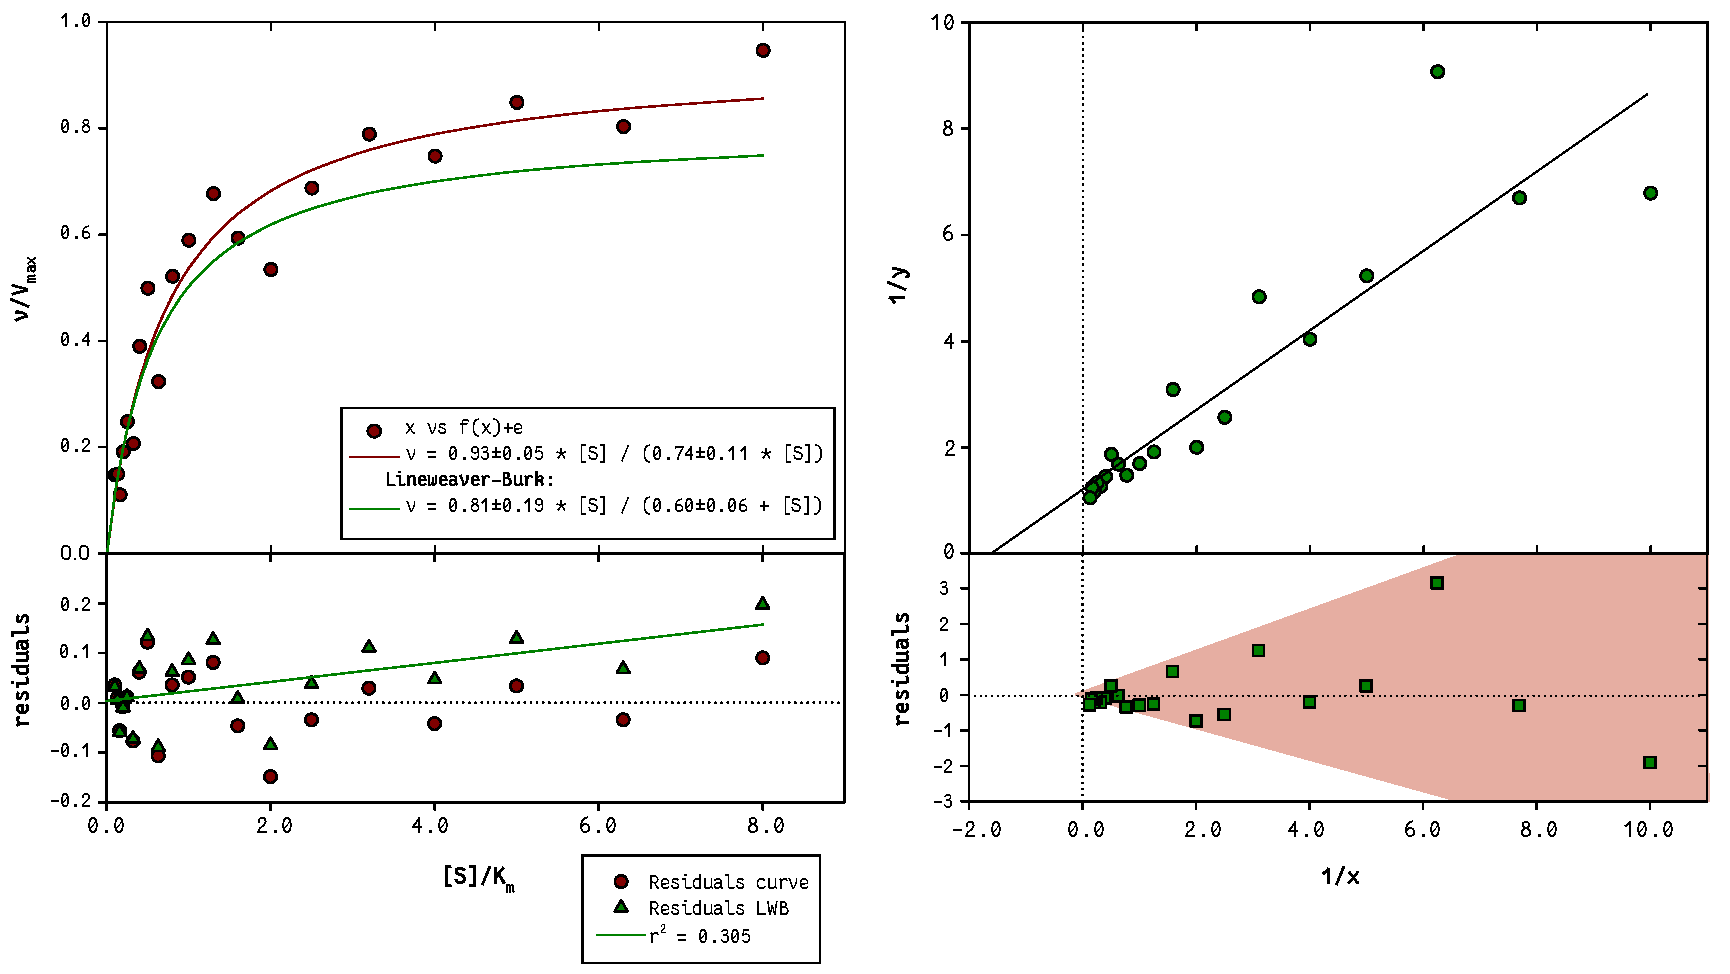
\includegraphics[width=\textwidth]{Graphics/LinearisingRegression}
\end{figure}

\begin{figure}
 \caption{\emph{Top}: Distribution of \num{200} normally distributed random figures. \emph{Bottom}: The distribution of the same data after taking reciprocals. The reciprocal of a \Name{Gauss}ian is not \Name{Gauss}ian!}
 \label{fig:RecGau}
 \centering
 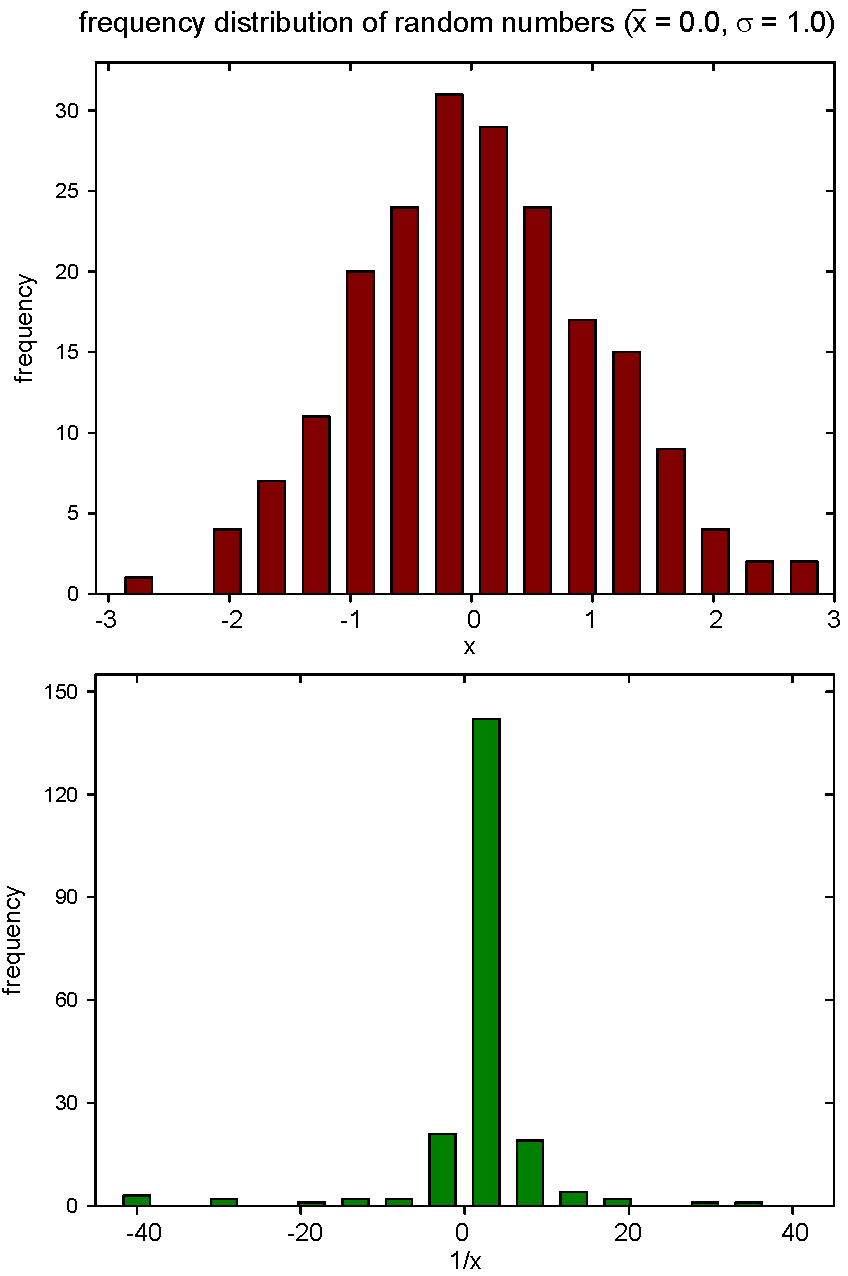
\includegraphics[width=0.75\textwidth]{Graphics/Reciprocal-Gaussian}
\end{figure}

Before computers became generally available, which allowed curve fitting by iterative methods, regression to suitably transformed data was generally used for curve fitting. The biggest disadvantage of these methods was that any method that transforms \AbsVec{y}, implicitly also transforms its error distribution. As a consequence, the requirements of homoscedasticity (see fig. \ref{fig:LinReg}) and of normality (see fig. \ref{fig:RecGau}) are violated, leading to biased estimates of parameters and, more importantly, their standard deviation. Note that this applies only to transformations of the dependent variable, as the independent variable is assumed to be error free its error distribution cannot be affected by transformation. Plots of transformed data still have a place in science for presentation purposes, as the human eye is very sensitive to deviations from a straight line. However, regression analysis of such data is largely obsolete.

Iterative regression methods require starting estimates of the parameters that should be reasonably close to the final value, firstly to reduce the number of iterations required and hence computer time. Secondly, iterative methods can become trapped in local minima of the error function, and then deliver suboptimal results. In my experience, the \Name{Levenberg-Marquardt}-algorithm \parencite{Lev-44,Mar-63} is more sensitive to this than \Name{Nelder-Mead}'s simplex algorithm \parencite{Nel-65,Cac-84,Kim-97}. Although the parameter estimates from linearising regression are biased, they are certainly good enough as starting values for iterative methods.

\begin{sidewaystable}
 \caption{Equations used in linearising regression. For the top equations, regression can happen directly, the bottom equations require an estimated parameter, either the \(y_\mathrm{max} \) or \(y_{x=0} \), respectively. The weights can be used to counteract the effect of the transformation on the error of the \AbsVec{y}-value.}
 \label{tab:linearise}
 \centering
 \begin{tabular}{rllllllll}
 \toprule
 No & Name                & Equation             & x-transform         & y-transform                                 & weight                                                    & \(a = \)            & \(b = \)       & \(m = \)  \\
 \midrule
  0 & Line through origin & \(y=b*x \)              & \(x^* = x \)            & \(y^* = y \)                                  & 1                                                         & \(a^* \)            & \(b^* \)       &        \\
  1 & linear              & \(y=a + b*x \)          & \(x^* = x \)            & \(y^* = y \)                                  & 1                                                         & \(a^* \)            & \(b^* \)       &        \\
  2 & exponential         & \(y=a*e^{m*x} \)        & \(x^* = x \)            & \(y^* = \ln(y) \)                             & \(y^2 \)                                                     & \(\exp(a^*) \)      &             & \(b^* \)  \\
  3 & power               & \(y=a*x^m \)            & \(x^* = \ln(x) \)       & \(y^* = \ln(y) \)                             & \(y^2 \)                                                     & \(\exp(a^*) \)      &             & \(b^* \)  \\
  4 & hyperbolic          & \(y=(a*x)/(b+x) \)      & \(x^* = 1/x \)          & \(y^* = 1/y \)                                & \(y^4 \)                                                     & \(1/a^* \)          & \(b^* a \)     &        \\
  5 & modif.invers        & \(y=a/(b+x) \)          & \(x^* = x \)            & \(y^* = 1/y \)                                & \(y^4 \)                                                     & \(1/b^* \)          & \(a^* a \)     &        \\
  6 & maximum             & \(y=a*x*e^{m*x} \)      & \(x^* = x \)            & \(y^* = \ln(x/y) \)                           & \((x * y)^2 / (y - x)^2 \)                                   & \(\exp(-a^*) \)     &             & \(-b^* \) \\
 \midrule
  7 & sigmoidal           & \(y=a/(1+b*x^m) \)      & \(x^* = \ln(x) \)       & \(y^* = \ln(y_\mathrm{max}/y - 1) \)          & \((y_\mathrm{max}/y - 1)^2 / (y_\mathrm{max} / y^2)^2 \)     & \(y_\mathrm{max} \) & \(\exp(a^*) \) & \(b^* \)  \\
  8 & exp.sigmoidal       & \(y=a/(1+b*exp(m*x)) \) & \(x^* = x \)            & \(y^* = \ln(y_\mathrm{max}/y - 1) \)          & \((y_\mathrm{max}/y - 1)^2 / (y_\mathrm{max} / y^2)^2 \)     & \(y_\mathrm{max} \) & \(\exp(a^*) \) & \(b^* \)  \\
  9 & mod. power          & \(y=a*x^m +b \)         & \(x^* = \ln(x) \)       & \(y^* = \ln(y - y_{x=0}) \)                   & \((y - y_{x=0})^2 \)                                         & \(y_{x=0} \)        & \(\exp(a^*) \) & \(b^* \)  \\
 10 & Hill                & \(y=a*x^m / (b+x^m) \)  & \(x^* = \log_{10}(x) \) & \(y^* = \log_{10}(y/ (y_\mathrm{max} - y)) \) & \(y^2 / \log_{10}(\mathrm{e} * (y_\mathrm{max}^2 - y))^2 \)  & \(y_\mathrm{max} \) & \(10^{-a} \)   & \(b^* \)  \\
 \bottomrule
 \end{tabular}
\end{sidewaystable}

\begin{lstlisting}[caption=Linearisation of curved data]
  PROCEDURE Transformation(CONST xOrig, yOrig : VectorTyp; VAR xTrans, yTrans : VectorTyp;
                           ct : CurveTyp; Schaetzwert : double);
  // transformation OF x, y TO linearise

  VAR i, n : INTEGER;

  BEGIN
      n := VectorLength(xOrig);
      CreateVector(xTrans, n, 0.0);
      CreateVector(yTrans, n, 0.0);
      FOR i := 1 TO n DO
        IF IsNaN(GetVectorelement(xOrig, i))
          THEN
            SetVectorElement(xTrans, i, NaN)
          ELSE
            CASE ct OF                        {Transformation of x-values}
              Origin, Linear, Exponential, Inverse, Maximum, ExpSigmoidal :
                 SetVectorElement(xTrans, i, GetVectorElement(xOrig, i));
              Power, Sigmoidal, ModPower :
                 SetVectorElement(xTrans, i, Ln(GetVectorElement(xOrig, i)));
              Hyperbola :
                 SetVectorElement(xTrans, i, 1 / GetVectorElement(xOrig, i));
              Hill :
                 SetVectorElement(xTrans, i, log(GetVectorElement(xOrig, i), 10));
            END;
      FOR i := 1 TO n DO
        IF IsNaN(GetVectorelement(yOrig, i))
          THEN
            SetVectorElement(yTrans, i, NaN)
          ELSE
            CASE ct OF                 {Transformation of y-values}
              Origin, Linear          :  SetVectorElement(yTrans, i, GetVectorElement(yOrig, i));
              Exponential, Power      :  SetVectorElement(yTrans, i, Ln(GetVectorElement(yOrig, i)));
              Hyperbola, Inverse      :  SetVectorElement(yTrans, i, 1 / GetVectorElement(yOrig, i));
              Maximum                 :  IF IsNaN(GetVectorelement(xOrig, i))
                                           THEN SetVectorElement(yTrans, i, NaN)
                                           ELSE SetVectorElement(yTrans, i, Ln(GetVectorElement(xOrig, i) / GetVectorElement(yOrig, i)));
              Sigmoidal, ExpSigmoidal :  SetVectorElement(yTrans, i, Ln(Schaetzwert / GetVectorElement(yOrig, i) - 1));
              ModPower                :  SetVectorElement(yTrans, i, Ln(GetVectorElement(yOrig, i) - Schaetzwert));
              Hill                    :  SetVectorElement(yTrans, i, log(GetVectorElement(yOrig, i) / (Schaetzwert - GetVectorElement(yOrig, i)), 10));
            END;
  END;


  PROCEDURE Retransform (CONST x, yTrans : Vectortyp; VAR TRes, Res : ResultTyp;
                         ct : CurveTyp; Schaetzwert : double;
                         VAR yCalc : VectorTyp);

  VAR i, n : WORD;

  BEGIN
    n := VectorLength(x);
    CreateVector(yCalc, n, 0.0);
    CASE ct OF
      Origin, Linear : BEGIN
                         CopyVector(yTrans, yCalc);
                         Res := TRes;
                         Res.m := 0;
                         Res.sm := 0;
                       END;
      Exponential    : BEGIN
                         Res.a  := Exp(TRes.a);
                         Res.sa := TRes.sa/Tres.a * Res.a;
                         Res.b  := 0;
                         Res.sb := 0;
                         Res.m  := TRes.b;
                         Res.sm := TRes.sb;
                         CreateVector(yCalc, VectorLength(yTrans), 0.0);
                         FOR i := 1 TO n DO
                           BEGIN
                             IF IsNaN(GetVectorElement(yTrans, i))
                               THEN SetVectorElement(yCalc, i, NaN)
                               ELSE SetVectorElement(yCalc, i, Res.a *
                                      Exp(Res.m * GetVectorElement(x, i)));
                           END;
                       END;
      Power          : BEGIN
                         Res.a  := Exp(TRes.a);
                         Res.sa := TRes.sa/Tres.a * Res.a;
                         Res.b  := 0;
                         Res.sb := 0;
                         Res.m  := TRes.b;
                         Res.sm := TRes.sb;
                         CreateVector(yCalc, VectorLength(yTrans), 0.0);
                         FOR i := 1 TO n DO
                           BEGIN
                             IF IsNaN(GetVectorElement(yTrans, i))
                               THEN SetVectorElement(yCalc, i, NaN)
                               ELSE SetVectorElement(yCalc, i, Res.a *
                                      Pot(GetVectorElement(x, i), Res.m)) ;
                           END;
                       END;
      Hyperbola      : BEGIN
                         Res.a  := 1/TRes.a;
                         Res.sa := TRes.sa/Tres.a * Res.a;
                         Res.b  := Tres.b * Res.a;
                         Res.sb := TRes.sb/Tres.b * Res.b;
                         Res.m  := 0;
                         Res.sm := 0;
                         CreateVector(yCalc, VectorLength(yTrans), 0.0);
                         FOR i := 1 TO n DO
                           BEGIN
                             IF IsNaN(GetVectorElement(yTrans, i))
                               THEN SetVectorElement(yCalc, i, NaN)
                               ELSE SetVectorElement(yCalc, i, Res.a * GetVectorElement(x, i)
                                       / (Res.b + GetVectorElement(x, i)));
                           END;
                       END;
      Inverse        : BEGIN
                         Res.a  := 1/TRes.b;
                         Res.sa := TRes.sb/Tres.b * Res.a;
                         Res.b  := Tres.a * Res.a;
                         Res.sb := TRes.sa/Tres.a * Res.b;
                         Res.m  := 0;
                         Res.sm := 0;
                         CreateVector(yCalc, VectorLength(yTrans), 0.0);
                         FOR i := 1 TO n DO
                           BEGIN
                             IF IsNaN(GetVectorElement(yTrans, i))
                               THEN SetVectorElement(yCalc, i, NaN)
                               ELSE SetVectorElement(yCalc, i, Res.a /
                                      (Res.b + GetVectorElement(x, i)));
                           END;
                       END;
      Maximum        : BEGIN
                         Res.a  := Exp(-TRes.a);
                         Res.sa := Abs(TRes.sa/Tres.a * Res.a);
                         Res.b  := 0;
                         Res.sb := 0;
                         Res.m  := -TRes.b;
                         Res.sm := Abs(TRes.sb/Tres.b * Res.m);
                         CreateVector(yCalc, VectorLength(yTrans), 0.0);
                         FOR i := 1 TO n DO
                           BEGIN
                             IF IsNaN(GetVectorElement(yTrans, i))
                               THEN SetVectorElement(yCalc, i, NaN)
                               ELSE SetVectorElement(yCalc, i, Res.a * GetVectorElement(x, i)
                                       * Exp(Res.m * GetVectorElement(x, i)));
                           END;
                       END;
      Sigmoidal      : BEGIN
                         Res.a  := Schaetzwert;
                         Res.sa := NaN;
                         Res.b  := Exp(TRes.a);
                         Res.sb := TRes.sa/Tres.a * Res.a;
                         Res.m  := TRes.b;
                         Res.sm := TRes.sb/Tres.b * Res.m;
                         CreateVector(yCalc, VectorLength(yTrans), 0.0);
                         FOR i := 1 TO n DO
                           BEGIN
                             IF IsNaN(GetVectorElement(yTrans, i))
                               THEN SetVectorElement(yCalc, i, NaN)
                               ELSE SetVectorElement(yCalc, i, Res.a /
                                      (1 + Res.b * Pot(GetVectorElement(x, i), Res.m)));
                           END;
                       END;
      ExpSigmoidal   : BEGIN
                         Res.a  := Schaetzwert;
                         Res.sa := NaN;
                         Res.b  := Exp(TRes.a);
                         Res.sb := TRes.sa/Tres.a * Res.a;
                         Res.m  := TRes.b;
                         Res.sm := TRes.sb/Tres.b * Res.m;
                         CreateVector(yCalc, VectorLength(yTrans), 0.0);
                         FOR i := 1 TO n DO
                           BEGIN
                             IF IsNaN(GetVectorElement(yTrans, i))
                               THEN SetVectorElement(yCalc, i, NaN)
                               ELSE SetVectorElement(yCalc, i, Res.a /
                                      (1 + Res.b * Exp(GetVectorElement(x, i) * Res.m)));
                           END;
                       END;
      ModPower       : BEGIN
                         Res.a  := Schaetzwert;
                         Res.sa := NaN;
                         Res.b  := Exp(TRes.a);
                         Res.sb := TRes.sa/Tres.a * Res.a;
                         Res.m  := TRes.b;
                         Res.sm := TRes.sb/Tres.b * Res.m;
                         CreateVector(yCalc, VectorLength(yTrans), 0.0);
                         FOR i := 1 TO n DO
                           BEGIN
                             IF IsNaN(GetVectorElement(yTrans, i))
                               THEN SetVectorElement(yCalc, i, NaN)
                               ELSE SetVectorElement(yCalc, i, Res.a + Res.b *
                                      Pot(GetVectorElement(x, i), Res.m));
                           END;
                       END;
      Hill           : BEGIN
                         Res.a  := Schaetzwert;
                         Res.sa := NaN;
                         Res.b  := pot(10, -TRes.a);
                         Res.sb := Abs(TRes.sa/Tres.a * Res.a);
                         Res.m  := TRes.b;
                         Res.sm := TRes.sb/Tres.b * Res.m;
                         CreateVector(yCalc, VectorLength(yTrans), 0.0);
                         FOR i := 1 TO n DO
                           BEGIN
                             IF IsNaN(GetVectorElement(yTrans, i))
                               THEN SetVectorElement(yCalc, i, NaN)
                               ELSE SetVectorElement(yCalc, i, Res.a * pot(GetVectorElement(x, i), Res.m)
                                      / (Res.b + Pot(GetVectorElement(x, i), Res.m)));
                           END;
                       END;
    END; // CASE
    Res.r := TRes.r;
    Res.t := TRes.t;
    Res.P0 := TRes.P0;
  END;
\end{lstlisting}


\section{\Name{Deming}-regression}\label{sec:Deming}

\begin{figure}
 \caption{\Name{Deming}-regression of an artificial data set with random noise. \emph{Top}: The data and the results of standard and \Name{Deming}-regression. \emph{Bottom}: Effect of \Name{Deming}-regression on the noise of the \AbsVec{x}- (\emph{left}) and \AbsVec{y}-data (\emph{right}). The regression results are closer to the line through the origin than the noisy data were. }
 \label{fig:Deming}
 \centering
 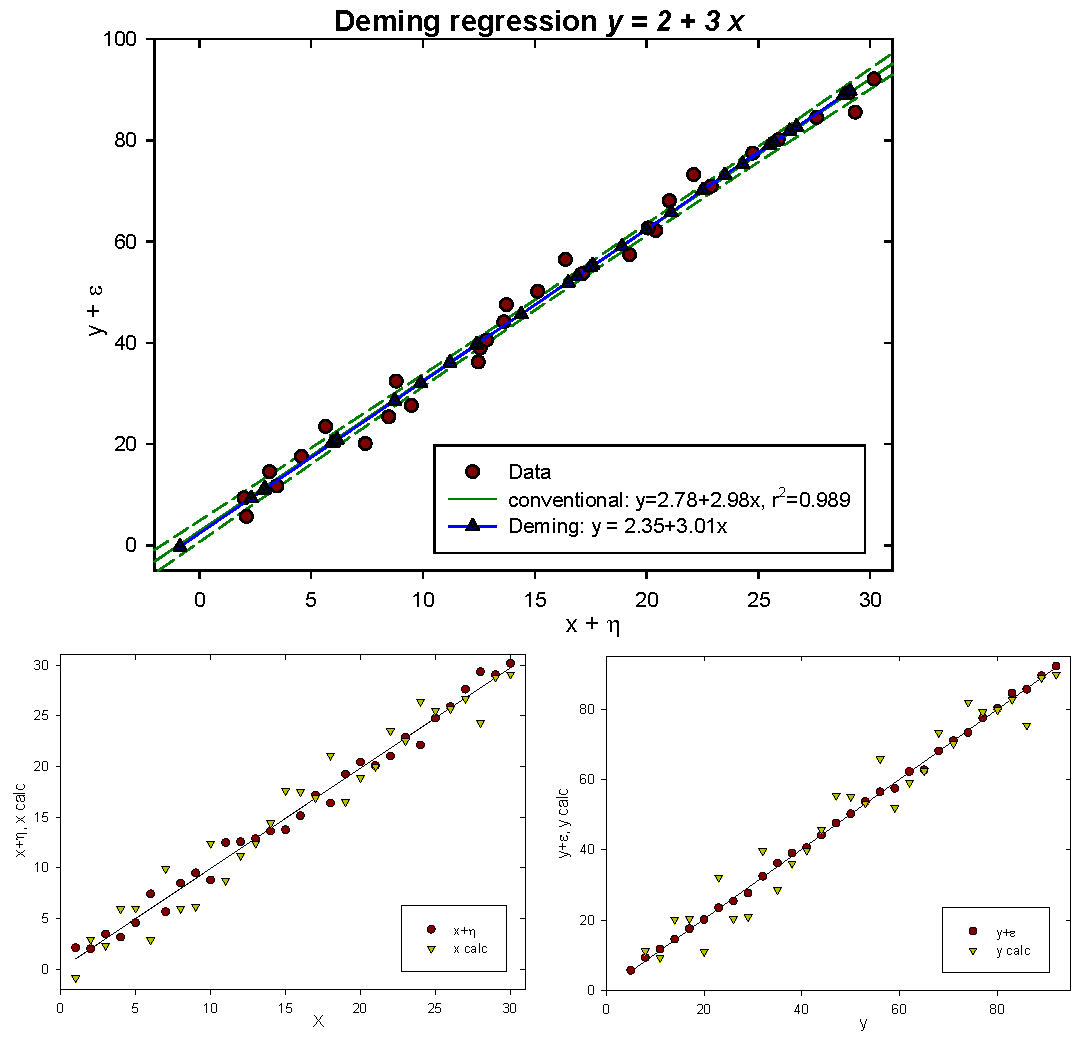
\includegraphics[width=0.75\textwidth]{Graphics/Deming}
\end{figure}

A \Name{Deming}-regression \parencite{Adc-78,Kum-79,Dem-43} is used when both dependent and independent variable have errors (see fig. \ref{fig:Deming}). The errors of dependent and independent variable are assumed independent, normally distributed, and with known ratio of their variance:
\begin{align}
  \AbsVec{y}_i &= \AbsVec{y}_i^* + \epsilon_i \\
  \AbsVec{x}_i &= \AbsVec{x}_i^* + \eta_i \\
  \delta &= \frac{\sigma_\epsilon^2}{\sigma_\eta^2}
\end{align}
The most common problem is that \skalar{\delta} is unknown. In the special case \(\delta = 1 \), \Name{Deming}-regression becomes orthogonal regression, which minimises the sum of squared distances between data points and regression line perpendicular to the line.

As estimate for \( \epsilon \) and \( \eta \) we can use the reciprocals of the reading error (obtained by error propagation, where necessary), divided by \(\sqrt{k} \) if they are the average of \( k \) measurements.

Then the weighted sum of squared distances is minimised
\begin{equation}
  \mathrm{RSS} = \sum_{i=1}^n\left(\frac{\epsilon_i^2}{\sigma^2_\epsilon} + \frac{\eta_i^2}{\sigma^2_\eta}\right)
               = \frac{1}{\sigma^2_\epsilon} \sum_{i=1}^n\left((\AbsVec{y}_i - \beta_0 - \beta_1 \AbsVec{x}_i^*)^2 + \delta (\AbsVec{x}_i - \AbsVec{y}_i^*)^2\right)
\end{equation}
With \(s_\AbsVec{xx} = 1/n \sum_{i=1}^n(\AbsVec{x}_i - \bar{\AbsVec{x}})^2 \) the sample variance of \AbsVec{x}, \(s_\AbsVec{yy} = 1/n \sum_{i=1}^n(\AbsVec{y}_i - \bar{\AbsVec{y}})^2 \) the sample variance of \AbsVec{y}, and \(s_\AbsVec{xy} = 1/n \sum_{i=1}^n\left((\AbsVec{x}_i - \bar{\AbsVec{x}})(\AbsVec{y}_i - \bar{\AbsVec{y}})\right) \)  the sample covariance of \AbsVec{x,y}. Note the small s, which distinguishes these second order moments from the first order ones used above.

We then get
\begin{align}
  b              &= \frac{s_\AbsVec{yy} - \delta s_\AbsVec{xx} + \sqrt{(s_\AbsVec{yy} - \delta s_\AbsVec{xx})^2 + 4 \delta s^2_\AbsVec{xy}}}{2 s_\AbsVec{xy}} \\
  a              &= \bar{\AbsVec{y}} - b \bar{\AbsVec{x}}  \\
  \hat{\AbsVec{x}}_i &= \AbsVec{x}_i + \frac{b}{b^2 + \delta}(\AbsVec{y}_i - a - b\AbsVec{x}_i)\\
\end{align}

The errors of the parameters are not available analytically and must be determined by bootstrapping.

\begin{lstlisting}[caption=Deming-regression]
  PROCEDURE Deming (CONST x, y : VectorTyp; delta : double;
                    VAR xCalc, yCalc : VectorTyp; VAR Res : ResultTyp);

  VAR i, n, s                                : WORD;
      Sx, Sy, sxx, syy, sxy, xMean, yMean,b_ : double;
      Significance                           : SignificanceType;
      c                                      : CHAR;

  BEGIN
    IF VectorLength(x) <> VectorLength(y)
      THEN
        BEGIN
          RegressionError := TRUE;
          c := WriteErrorMessage('Deming regression: unequal length of data vectors');
          EXIT;
        END;
    n := VectorLength(x);
    s := 0;                                                   // calculate means
    Sx := 0;
    Sy := 0;
    FOR i := 1 TO n DO
      BEGIN
        IF IsNaN(GetVectorElement(x, i)) OR IsNaN(GetVectorElement(y, i))
          THEN
          ELSE
            BEGIN
              INC(s);                                        // valid data pairs
              Sx := Sx + GetVectorElement(x, i);
              Sy := Sy + GetVectorElement(y, i);
            END;
      END;
    xMean := Sx / s;                                    // calculate 2nd moments
    yMean := Sy / s;
    sxx := 0;
    syy := 0;
    sxy := 0;
    FOR i := 1 TO n DO
      BEGIN
        IF IsNaN(GetVectorElement(x, i)) OR IsNaN(GetVectorElement(y, i))
          THEN
          ELSE
            BEGIN
              sxx := sxx + Sqr(GetVectorElement(x, i) - xMean);
              syy := syy + Sqr(GetVectorElement(y, i) - yMean);
              sxy := sxy + (GetVectorElement(x, i) - xMean) * (GetVectorElement(y, i) - yMean)
            END;
      END;
     sxx := sxx/s; // sample variance x
     syy := syy/s; // sample variance y
     sxy := sxy/s; // sample covariance x,y                  // calculate params
     Res.b := (syy - delta*sxx + Sqrt((syy-delta*sxx)*(syy-delta*sxx) + 4*delta*sxy*sxy))
               / (2*sxy);
     Res.sb := NaN; // Deming regression doesn't provide error estimates
     Res.a := yMean - Res.b*xMean;
     Res.sa := NaN;
     Res.r := QuadrantCorrelation(x, y, Significance);
     Res.P0 := Significance.P0;
     Res.t := Significance.Testvalue; // actually chi^2, not t
     CreateVector(xCalc, n, 0.0);                    // calculate xCalc and yCalc
     CreateVector(yCalc, n, 0.0);
     b_ := Res.b/(Res.b*Res.b + delta);
     FOR i := 1 TO n DO
       BEGIN
         IF IsNaN(GetVectorElement(x, i)) OR IsNaN(GetVectorElement(y, i))
           THEN
           ELSE
             BEGIN
               SetVectorElement(xCalc, i, GetVectorElement(x, i) + (GetVectorElement(y, i) -
                                Res.a - Res.b * GetVectorElement(x, i)));
               SetVectorElement(yCalc, i, Res.a + Res.b * GetVectorElement(xCalc, i));
             END;
       END;
  END;
\end{lstlisting}

\section{\Name{Theil-Sen-Kendall}-estimator for noisy data}

In this method \parencite{The-50}, the median of the slopes of all \( n(n-1)/2 \) lines connecting two data points ( \( (\AbsVec{y}_j - \AbsVec{y}_i)/(\AbsVec{x}_j - \AbsVec{x}_i)\ \forall\ i,j \in [1\ldots n], i \neq j, \AbsVec{x}_j \neq \AbsVec{x}_i \)) is taken as slope of the regression line \skalar{b}. The last condition is relevant when replicate data are available for the same \AbsVec{x}. Since the determination of slope is the more precise, the larger the difference \(\abs(\AbsVec{x}_j - \AbsVec{x}_i) \) is, one can test for a minimal difference rather than for a difference of zero. The average distance is \(\frac{\max(\AbsVec{x}) - \min(\AbsVec{x})}{n} \), so the significant distance is chosen lower by some arbitrary factor.

The intercept is calculated from \(a = \tilde{\AbsVec{y}} - b \tilde{\AbsVec{x}} \). The alternative estimator for \skalar{a}, the median of the intercept of all the lines, is less robust.

It is possible to weigh the slopes by \(\AbsVec{x}_1 - \AbsVec{x}_2 \) on the grounds that larger distances allow a more accurate determination of slopes.

An estimate for the imprecision of slope and intercept can be calculated from their interquartile distance: \((Q_3 - Q_1) / 2 \). This is similar to the standard deviation in least squares regression, except that it includes the centre \SI{50}{\%} rather than \SI{68}{\%} of values. Similar again to linear regression, estimates of error require sufficient data, \(n > 600 \), to be meaningful.

The \Name{Theil-Sen-Kendall}-estimator has the following properties:
\begin{itemize}
  \item{The \Name{Kendall} \(\tau \) rank correlation coefficient between \(\AbsVec{x}_i \) and the corresponding residual \((\AbsVec{y}_i - \hat{\AbsVec{y}}_i) \) is approximately zero, that is, the probability of a point being above or below the regression line does not depend on \(\AbsVec{x}_i \).}
  \item{The median of the residuals is approximately zero; that is, the fit line passes above and below equal numbers of points. }
  \item{The estimates are more robust against noise than the least squares estimator, \(1 - 1/\sqrt{2} \approx \SI{30}{\%} \) of the data may be arbitrarily corrupted before accuracy drops.}
  \item{The non-parametric \Name{Theil-Sen-Kendall}-estimator is almost as efficient as the parametric least squares method in the absence of outliers and normality violations, and much better is these conditions are not met.}
\end{itemize}

An even more robust method for slope calculation is to calculate first the median of all lines going through an \(\AbsVec{x}_i \), and then calculate the median of those for all \AbsVec{x}  \parencite{Sie-82}. The breakdown point of this method is \SI{50}{\%} corrupted data. However, this method is computationally more expensive, it also requires repeat measurements for each \(\AbsVec{x}_i \).

With the \Name{Theil-Sen-Kendall}-estimator being a non-parametric method of linear regression, it makes sense to also use a non-parametric correlation coefficient, here the quadrant correlation (see subsection \ref{text:quadrant} on page \pageref{text:quadrant}). The significance of \texttt{Res.P0} is calculated from a \(\chi^2 \) test with \(\nu = 1 \), thus \texttt{Res.t} actually contains \(\chi^2 \).

\begin{lstlisting}[caption=Theil-Sen-Kendall-estimator]
  PROCEDURE TheilSenKendall (CONST x, y : VectorTyp; VAR yCalc : VectorTyp;
                             VAR Res : ResultTyp);

  VAR i, j, n, s                                                       : WORD;
      Slopes, Slopes_big, Intercepts, Intercepts_big, xSorted, ySorted : VectorTyp;
      x1, x2, y1, y2, xmin, xmax, xdiff, Sx, Sy, xMed, yMed            : double;
      Significance                                                     : SignificanceType;
      c                                                                : CHAR;
      unknown                                                          : BOOLEAN;

  BEGIN
    IF VectorLength(x) <> VectorLength(y)
      THEN
        BEGIN
          RegressionError := TRUE;
          c := WriteErrorMessage('Linear regression: unequal Length OF dependent AND independent data vector');
          EXIT;
        END;
    n := VectorLength(x);
    s := 0;
    CreateVector(Slopes_big, Round(n*(n-1)/2 + 0.5), 0.0);   // maximal possible number OF slopes
    xmax := FindLargest(x);
    xmin := FindSmallest(x);
    xdiff := (xmax - xmin) / (5 * n);  // factor 5 IS arbitrary
    FOR i := 1 TO n DO
       FOR j := Succ(i) TO n DO
         BEGIN
           x1 := GetVectorElement(x, i);
           x2 := GetVectorElement(x, j);
           y1 := GetVectorElement(y, i);
           y2 := GetVectorElement(y, j);
           unknown :=  IsNaN(x1) OR IsNaN(x2) OR  IsNaN(y1) OR IsNaN(y2);
           IF (Abs(x1 - x2) < xdiff) OR unknown
             THEN
             ELSE
               BEGIN
                 INC(s);
                 SetVectorElement(Slopes_big, s, (y1-y2)/(x1-x2));
               END;
         END;
     CreateVector(slopes, s, 0.0);
     FOR i := 1 TO s DO  // remove any empty values from slope vector
       SetVectorElement(slopes, i, GetVectorElement(slopes_big, i));
     DestroyVector(Slopes_big);
     Res.b := Median(slopes);
     Res.sb := (Quantile(slopes, 0.75) - Quantile(slopes, 0.25)) / 2;
     CopyVector(x, xSorted);
     xMed := Median(xSorted);
     CopyVector(y, ySorted);
     yMed := Median(ySorted);
     Res.a := yMed - Res.b * xMed; // most stable estimator FOR intercept
     CreateVector(Intercepts_big, n, 0.0);
     s := 0;
     FOR i := 1 TO n DO  // calculate intercepts FOR all x/y pairs
       IF IsNan(GetVectorElement(x, i)) OR IsNaN(GetVectorElement(y, i))
         THEN
         ELSE
           BEGIN
             SetVectorElement(Intercepts_big, i, GetVectorElement(y, i) - Res.b * GetVectorElement(x, i));
             INC(s);
           END;
     CreateVector(Intercepts, s, 0.0);
     FOR i := 1 TO s DO  // remove any empty values from intercept vector
       SetVectorElement(Intercepts, i, GetVectorElement(Intercepts_big, i));
     DestroyVector(Intercepts_big);
     Res.sa := (Quantile(intercepts, 0.75) - Quantile(intercepts, 0.25)) / 2;
     Res.r := QuadrantCorrelation(x, y, Significance);
     Res.P0 := Significance.P0;
     Res.t := Significance.Testvalue; // actually chi^2, NOT t
     CreateVector(yCalc, n, 0.0);
     FOR i := 1 TO n DO
       SetVectorElement(yCalc, i, Res.a + Res.b * GetVectorElement(x, i));
     DestroyVector(xSorted);
     DestroyVector(ySorted);
     DestroyVector(Slopes);
     DestroyVector(Intercepts);
  END;
\end{lstlisting}

\section{The direct plot of \Name{Eisenthal \& Cornish-Bowden}}

\begin{sidewaysfigure}
 \caption{The direct plot of \Name{Eisenthal \& Cornish-Bowden} with pseudo-random noise added to a \Name{Henri-Michaelis-Menten}-curve with \(K_\mathrm{M} = 1.0 \) and \(V_\mathrm{max} = 1.0 \). \emph{Left}: Most lines intersect inside the red ellipse. \emph{Centre}: Distribution of estimates for \skalar{K_\mathrm{M}} and \skalar{V_\mathrm{max}} (extreme outliers not shown for clarity). Note how the outliers pull the arithmetic mean (\emph{dotted line}) outside the interquartile boxes. The median (\emph{drawn-out line}) is a much better estimator of position. \emph{Right}: Plot of data, estimated curve and residuals. Note also how even a modest amount of random noise pulls the estimates away from the ``true'' parameters, this effect is stronger for \skalar{K_\mathrm{M}} than for \skalar{V_\mathrm{max}}. }
 \label{fig:Eisenthal}
 \centering
 \subfloat{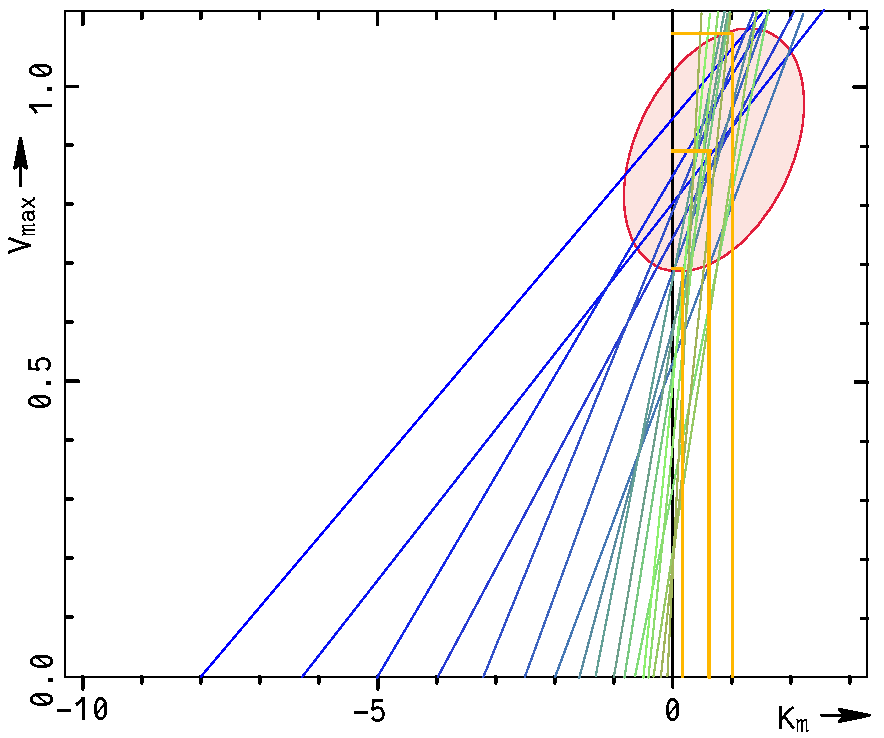
\includegraphics[width=0.3\textwidth]{Graphics/Eisenthal1}}\hfill
 \subfloat{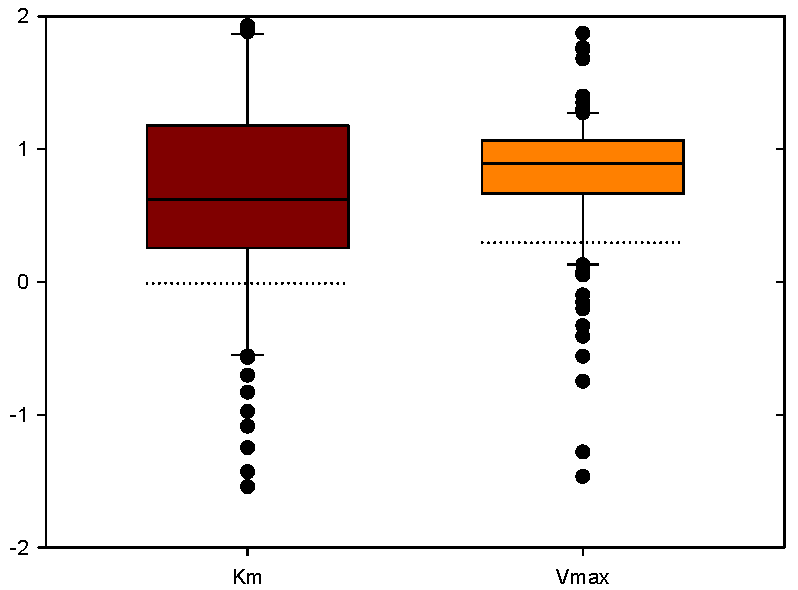
\includegraphics[width=0.3\textwidth]{Graphics/Eisenthal3}}\hfill
 \subfloat{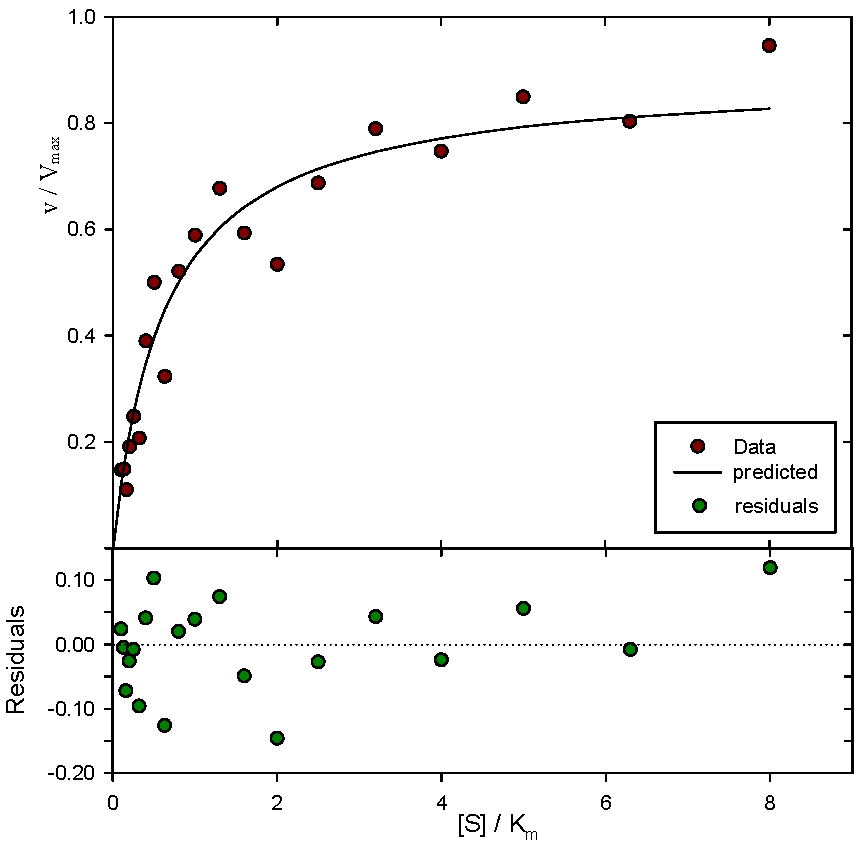
\includegraphics[width=0.3\textwidth]{Graphics/Eisenthal2}}\\
\end{sidewaysfigure}

This method is relevant for enzyme kinetics data, that is the measurement of the reaction velocity \skalar{v} as function of substrate concentration \skalar{[S]}, which is described by the \Name{Henri-Michaelis-Menten}- (HMM-) equation:
\begin{equation}
   v = \frac{V_\mathrm{max} [S]}{K_\mathrm{M} + [S]}
\end{equation}
As mentioned earlier, for such hyperbolic relationships linearising regression may be used, but with significant bias. In particular, estimates of the \Name{Michaelis}-constant \skalar{K_\mathrm{M}} is error-prone.

As \Name{Eisenthal \& Cornish-Bowden} \parencite{Eis-74,Cor-74} realised, if one places lines through the substrate concentrations on the \skalar{x}-axis and the corresponding velocity on the \skalar{y}-axis, all these lines should intersect at \((K_\mathrm{M}, V_\mathrm{max}) \). In practice, one gets a cloud of \(\frac{n (n-1)}{2} \)  intersection points due to experimental noise (see fig. \ref{fig:Eisenthal}). Thus, the median of all intersections between the lines can be used as an unbiased, non-parametric estimator for these two parameters.

The parameters can be calculated from any pair \skalar{i, j} of measured \([S], v \) by
 \begin{align}
   V_{i,j} &= \frac{[S]_i - [S]_j}{\frac{[S]_i}{v_i} - \frac{[S]_j}{v_j}} \\
   K_{i,j} &= \frac{v_j - v_i}{\frac{v_i}{[S]_i} - \frac{v_j}{[S]_j}}
 \end{align}

\begin{lstlisting}[caption=Direct plot]
PROCEDURE Eisenthal (CONST Substrate, Velocity : VectorTyp; VAR yCalc : VectorTyp;
                           VAR Res : ResultTyp);

VAR Km, Vmax, Km_big, Vmax_big : VectorTyp;
    i, j, n, s                 : WORD;
    c                          : CHAR;
    SI, vi, Sj, vj             : double;
    Significance               : SignificanceType;

BEGIN
  IF VectorLength(Substrate) <> VectorLength(Velocity)
    THEN
      BEGIN
        RegressionError := TRUE;
        c := WriteErrorMessage('Direct plot: unequal Length OF dependent AND independent data vector');
        EXIT;
      END;
  n := VectorLength(Substrate);
  s := 0;
  CreateVector(Km_big, Round(n*(n-1)/2 + 0.5), 0.0);   // maximal possible number OF pairs
  CreateVector(Vmax_big, Round(n*(n-1)/2 + 0.5), 0.0);
  FOR i := 1 TO n DO
     FOR j := Succ(i) TO n DO
       BEGIN
         SI := GetVectorElement(Substrate, i);
         Vi := GetVectorElement(Velocity, i);
         Sj := GetVectorElement(Substrate, j);
         Vj := GetVectorElement(Velocity, j);
         IF (IsNaN(SI) OR IsNaN(vi) OR  IsNaN(Sj) OR IsNaN(vj))
           THEN
             // ignore
           ELSE
             BEGIN
               INC(s);
               SetVectorElement(Km_big,   s, (vj - vi) / (vi/SI - vj/Sj));
               SetVectorElement(Vmax_big, s, (SI - Sj) / (SI/vi - Sj/vj));
             END;
       END;
   CreateVector(Km, s, 0.0);
   CreateVector(Vmax, s, 0.0);
   FOR i := 1 TO s DO  // remove any empty values from result vectors
     BEGIN
       SetVectorElement(Km, i, GetVectorElement(Km_big, i));
       SetVectorElement(Vmax, i, GetVectorElement(Vmax_big, i));
     END;
   DestroyVector(Km_big);
   DestroyVector(Vmax_big);
   Res.a := Median(Km);
   Res.sa := (Quantile(Km, 0.75) - Quantile(Km, 0.25)) / 2;
   Res.b := Median(Vmax);
   Res.sb := (Quantile(Vmax, 0.75) - Quantile(Vmax, 0.25)) / 2;
   FOR i := 1 TO s DO
     Writeln(i:3, ' ', GetVectorElement(Km, i):3:3, ' ', GetVectorElement(Vmax, i):3:3);
   Res.r := QuadrantCorrelation(Substrate, Velocity, Significance);
   Res.P0 := Significance.P0;
   Res.t := Significance.Testvalue; // actually chi^2, NOT t
   CreateVector(yCalc, n, 0.0);
   FOR i := 1 TO n DO
     BEGIN
       SI := GetVectorElement(Substrate, i);
       IF IsNaN(SI)
         THEN
           SetVectorElement(yCalc, i, NaN)
         ELSE
           SetVectorElement(yCalc, i, Res.b * SI / (Res.a + SI));
     END;
  DestroyVector(Km);
  DestroyVector(Vmax);
END;

END.
\end{lstlisting}

\section{Aberrant data points}

If the data set \AbsVec{x,y} contains outliers, that is, data points with an error much larger than the other points, the calculated slope will hardly be affected. However, the standard deviations for the parameters will be increased and \skalar{r} decreased. Such outliers should be identified and removed from the data set. On the other hand, data points with high leverage, that is, \skalar{\AbsVec{x}_i} is far away from \skalar{\bar{\AbsVec{x}}}, will strongly affect the parameters.

It is, however, important to use consistent rules for identification of aberrant points. Arbitrary removal of data points which may not fit with ones hypothesis will seriously bias the results and render them useless.

\subsection{Leverage points}

With
\begin{equation}\label{eqn:leverage}
  \arr{H} = \arr{X} (\arr{X}^T \arr{X})^{-1} \arr{X}^T
\end{equation}
the hat-matrix, its \skalar{i}th diagonal element \(\AbsVec{h}_{ii} \) is the \textbf{leverage} of \skalar{\AbsVec{x}_i}. It describes, how much this point will influence the calculated parameters of the regression and is largest for those \skalar{\AbsVec{x}_i} that are furthest away from \skalar{\bar{\AbsVec{x}}_i}. For a simple linear regression,
\begin{equation}
  \AbsVec{h}_{ii} = \frac{1}{n} - \frac{(\AbsVec{x}_i - \bar{\AbsVec{x}})^2}{\sum_{j=1}^n{(\AbsVec{x}_j - \bar{\AbsVec{x}})^2}}
\end{equation}
\( 0 \leq \AbsVec{h}_{ii} \leq 1 \) and any \( \AbsVec{h}_{ii} > \frac{3q}{n} \) is considered high leverage. \skalar{q} is the number of fitted parameters (including intercept).

With those definitions,
\begin{equation}
  \AbsVec{t}_i = \frac{\hat{\epsilon}_i}{\hat{\sigma} \sqrt{1-\AbsVec{h}_{ii}}}
\end{equation}
is called the \textbf{internally \Name{Student}ised residual}. If the absolute value of this residual for any data point exceeds 3, this point can be considered an outlier. If a data point is suspected of being an outlier, it should be excluded from the summation in eqn. \ref{eqn:sigma}, and \skalar{n} in its denominator must be decreased accordingly. However, before it is removed from the data set, make sure that it does not result from an incomplete model!

\subsection{Outliers}

Unlike the errors \(\epsilon_i \) of the measured \AbsVec{y}, the residuals \(\hat{\epsilon}_i = \AbsVec{y}_i - \hat{\AbsVec{y}}_i \) obtained from regression cannot be independent from each other, as their sum must equal zero. Their value decreases with increasing \(\AbsVec{x}_i - \bar{\AbsVec{x}} \). Their variance can be estimated as
\begin{equation}\label{eqn:sigma}
  \hat{\sigma}^2 = \frac{1}{(n-q)} \sum_{i=1}^n{\hat{\epsilon}_i^2} = \frac{1}{(n-q)} \sum_{i=1}^n{(\AbsVec{y}_i - \hat{\AbsVec{y}}_i)^2}
\end{equation}
with \skalar{q} the number of parameters.

\Name{Cook}'s distance is defined as
\begin{equation}
  D_i = \frac{(\hat{\beta} - \hat{\beta}^{\not i})^T (\arr{X}^T\arr{x}) (\hat{\beta} - \hat{\beta}_{\not i})^2}{(1+q) s^2}
      = \frac{\sum_{j=i}^n{(\bar{\AbsVec{y}}_j - \bar{\AbsVec{y}}_j^{\not i})}}{q \mathrm{MSE}}
\end{equation}
where \( \hat{\beta}_{\not i} \) is the calculated least squares slope and \( \bar{\AbsVec{y}}_j^{\not i} \) the calculated \AbsVec{y}  from a refitted regression model in which observation \skalar{i} has been omitted. \acs{MSE} the mean squared error. Values with a \Name{Cook}'s distance of more than four times the mean are suspicious, this measure is somewhat more sensitive than other measures of outliers.

\section{Shrinkage}

Sometimes, the relative importance of the variables in \arr{X} is unknown. In such cases, it is possible to constrain the sum of parameters \(\beta \), and thereby improve their variance \parencite[chapter 6]{Jam-13}.

\subsection{Ridge regression}

In ridge regression, we look for the minimum of
\begin{equation}
  \min\left[\sum_{i=1}^n{(\AbsVec{y}_i - \hat{\AbsVec{y}})^2} + \lambda \sum_{j=1}^p{\beta_j^2} \right]
\end{equation}
, that is, we minimise the sum of both the residual sum of squares and the \(\ell_2 \)-norm of the parameters (except intercept \(\beta_0 \)), \Foreign{i.e.}, the sum of their squares. The relative weight of the later, \textbf{the shrinkage penalty}, is determined by \(\lambda \in [0\ldots\infty] \). If \(\lambda = 0 \) we have a conventional least squares regression. As \(\lambda \) increases, the estimates for \(\beta_j \) are shrunk toward zero. For each \(\lambda \), there is a budget variable \(s \) so that \(\ell_2(\beta) \leq s \). For small \(\lambda \), \(s \) is large and not restrictive, but as \(\lambda \) increases, \(s \) becomes smaller and eventually limiting.

A least square fit has little bias, but may have a lot of variance, that is, a small change in the training data may result in a significant change of the estimated parameters. This variance increases with \(p \), if \(p > n \) regression isn't even possible. As \(\lambda \) increases, the flexibility of the regression decreases, increasing bias and decreasing variance. As the mean squared error \(\mathrm{MSE} = \frac{\sum{(\AbsVec{y}_i - \hat{\AbsVec{y}})^2}}{n} \) is a function of the sum of squared bias and variance, it has an optimal value at a particular \( \lambda \). Hence, the selection of \( \lambda \) is critical and performed by validation (see section \ref{text:validation} on page \pageref{text:validation}).

Before ridge regression, the data should be \AbsVec{z}-standardised so all variables are on the same scale (namely, standard deviations from mean). Otherwise, the final fit would depend on the scale at which the variables have been measured.

\subsection{Lasso regression}\label{text:lasso}

In ridge regression, all parameters are shrunk in the same way, in other words, ridge regression cannot distinguish between important and irrelevant variables. A small change in the equation rectifies this:
\begin{equation}
  \min\left[\sum_{i=1}^n{(\AbsVec{y}_i - \hat{\AbsVec{y}})^2} + \lambda \sum_{j=1}^p{|\beta_j|} \right]
\end{equation}
, in other words, we use the \(\ell_1 \)-, rather than the \(\ell_2 \)-norm of the parameters. This yields \textbf{sparse models}, that is, some parameters may be set to exactly zero. Their number depends on \(\lambda \).

\paragraph{Method selection:} Lasso regression performs slightly poorer than ridge regression when all predictor variables make a seizable contribution to the predicted variable (signal variables); it is superior when there are irrelevant variables (noise variables). A plot of \acs{MSE} \Foreign{vs} \( \lambda \) will show whether shrinkage should be used at all, or whether simple least square regression is sufficient for the problem. Ridge regression can also uncover correlations between variables (\textbf{grouping}). It is possible to combine lasso- and ridge-regression to \textbf{elastic net regression}:
\begin{equation}
  \min\left[\sum_{i=1}^n{(\AbsVec{y}_i - \hat{\AbsVec{y}})^2} + \lambda_1 \ell_1(\beta) + \lambda_2 \ell_2(\beta) \right]
\end{equation}

\printbibliography[heading=subbibliography]
\end{refsection}

  % -*- TeX:UK -*-
\chapter{Regression of curves: The simplex algorithm}\label{chap:Simplex}
\begin{refsection}

\abstract{The simplex algorithm is an iterative technique that can be used for any regression problem, from straight lines to curves of arbitrary complexity. The differential of the equation need not be known nor even exist. It is not limited to minimising the sum of squared residuals, but can use any optimisation criterium that is continuous. Minimum median residual is used for noisy data, minimum \(\chi^2 \) for heteroscedastic data. The biggest disadvantage of the simplex algorithm is that it does not directly produce error estimates for the parameters, these need to be obtained by bootstrapping. }

\section{How does the simplex algorithm work?}

\begin{figure}
 \caption{RSS of the data in fig. \ref{fig:LinReg} on page \pageref{fig:LinReg} as function of the values of the parameters. Each pair of parameters gives a RSS-value (colour-coded like a topographic map). The black triangles indicate the moves of the simplex from an arbitrary starting point, note how the simplex expands as it moves downhill and then contracts again near the minimum. For details see text. }
 \label{fig:ErrorSurface}
 \centering
 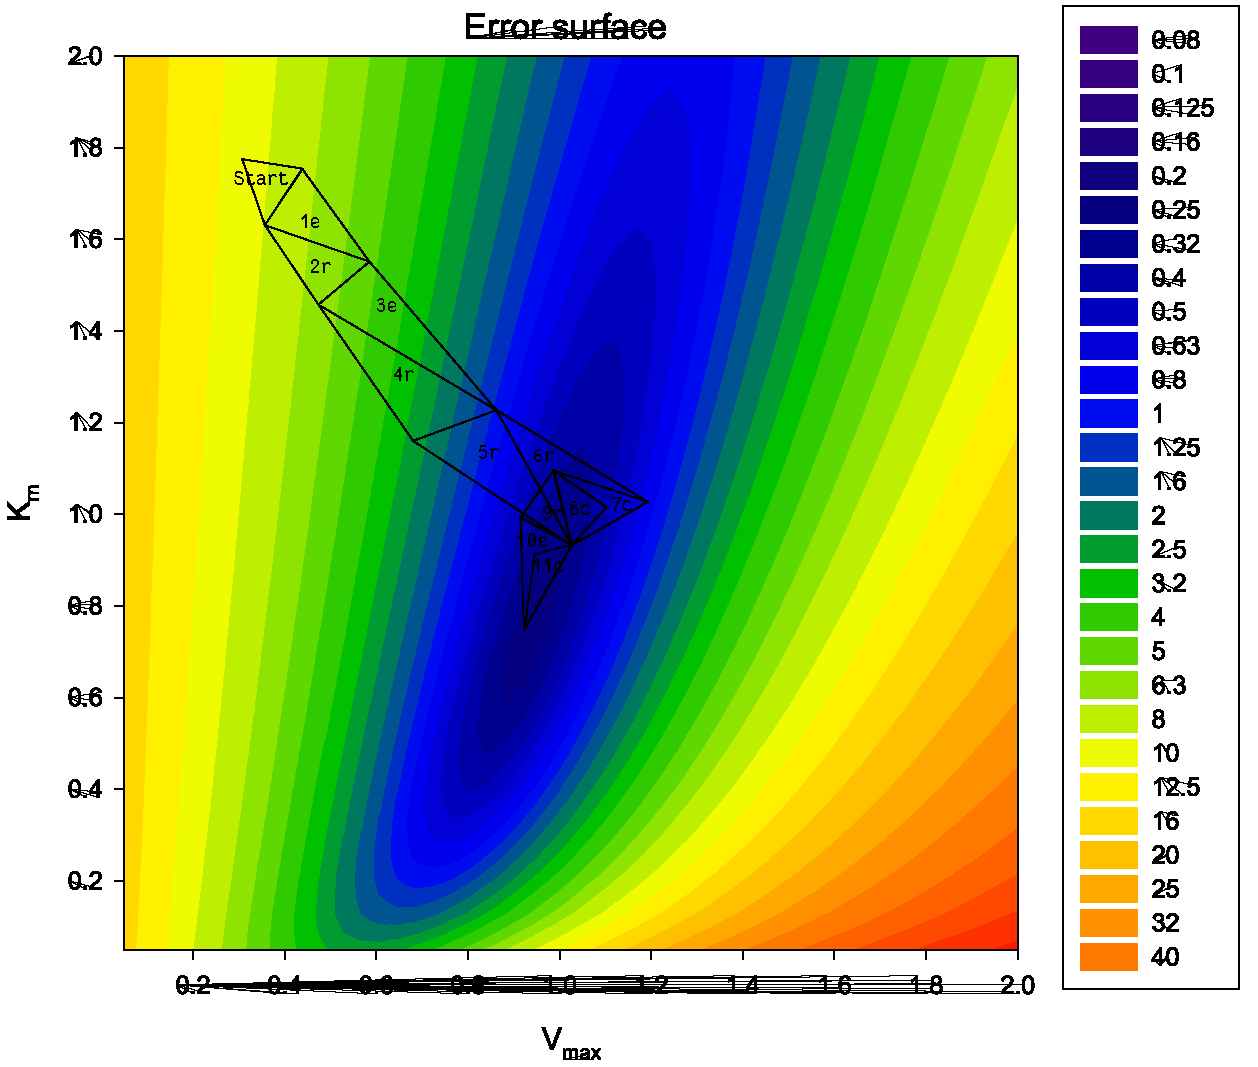
\includegraphics[width=\textwidth]{Graphics/ErrorSurface}
\end{figure}

Let us return to the example in fig. \ref{fig:LinReg} on page \pageref{fig:LinReg}, a \Name{Henri-Michaelis-Menten} curve with considerable scatter. We can now choose arbitrary pairs of the parameters, \skalar{V_\mathrm{max}} and \skalar{K_\mathrm{m}}, each such pair will give a \acf{RSS} (see fig. \ref{fig:ErrorSurface}). What we would like to find is the pair of parameters for which \acs{RSS} becomes minimal. All \acs{RSS}-values of all parameter sets (although we deal with two parameters here for ease of drawing, the method can handle an arbitrary number of parameters \skalar{p}, the error surface then has \(p+1 \) dimensions) together form the \textbf{error surface} of the problem. In effect, we look for way to take an arbitrary starting set of parameters and from there move ``downhill'' until we reached the minimum with sufficient precision. One way of doing this is to calculate the gradient (\skalar{\nabla},  multi-dimensional slope) of the function at your current estimate for the parameters and move downward in the direction to the \textbf{steepest descent} for a small distance, arriving at your new, improved estimate. This is repeated until further moves no longer reduce the \acs{RSS}, that is, until the gradient becomes close to zero. The \Name{Levenberg-Marquardt} \parencite{Lev-44,Mar-63} algorithm uses (in part) this method. However, this requires the error function not only to be continuously differentiable (without singularities as for example in \(f(x) = 1/x, x = 0 \)), but the first derivative must also be known (how good were you in calculus?). The main advantage of steepest descent methods is that since the gradient is known, it is easy to calculate error estimates for the found parameters directly.

The simplex algorithm \parencite{Nel-65,Cac-84,Kim-97} takes a geometric approach, and is therefore more generally applicable. Neither the regression function nor its error surface need to be differentiable, all that is required is that we can calculate the dependent variable \(\hat{\AbsVec{y}} \) for any data vector \(\AbsVec{x} \) and any parameter vector \(\beta \). The simplex method can minimise not only the \acs{RSS}, but also other error functions like \(\chi^2 \) or the median of residuals. This can be useful for non-homoscedastic or noisy data. However, simplex does not directly give error estimates for the parameters, these need be calculated from bootstrapping \parencite{Str-92,Str-10}.

\begin{figure}
 \caption{Possible movements of a simplex. The old simplex is in \emph{green}, the new in \emph{orange}. For details see text. }
 \label{fig:SimMo}
 \centering
 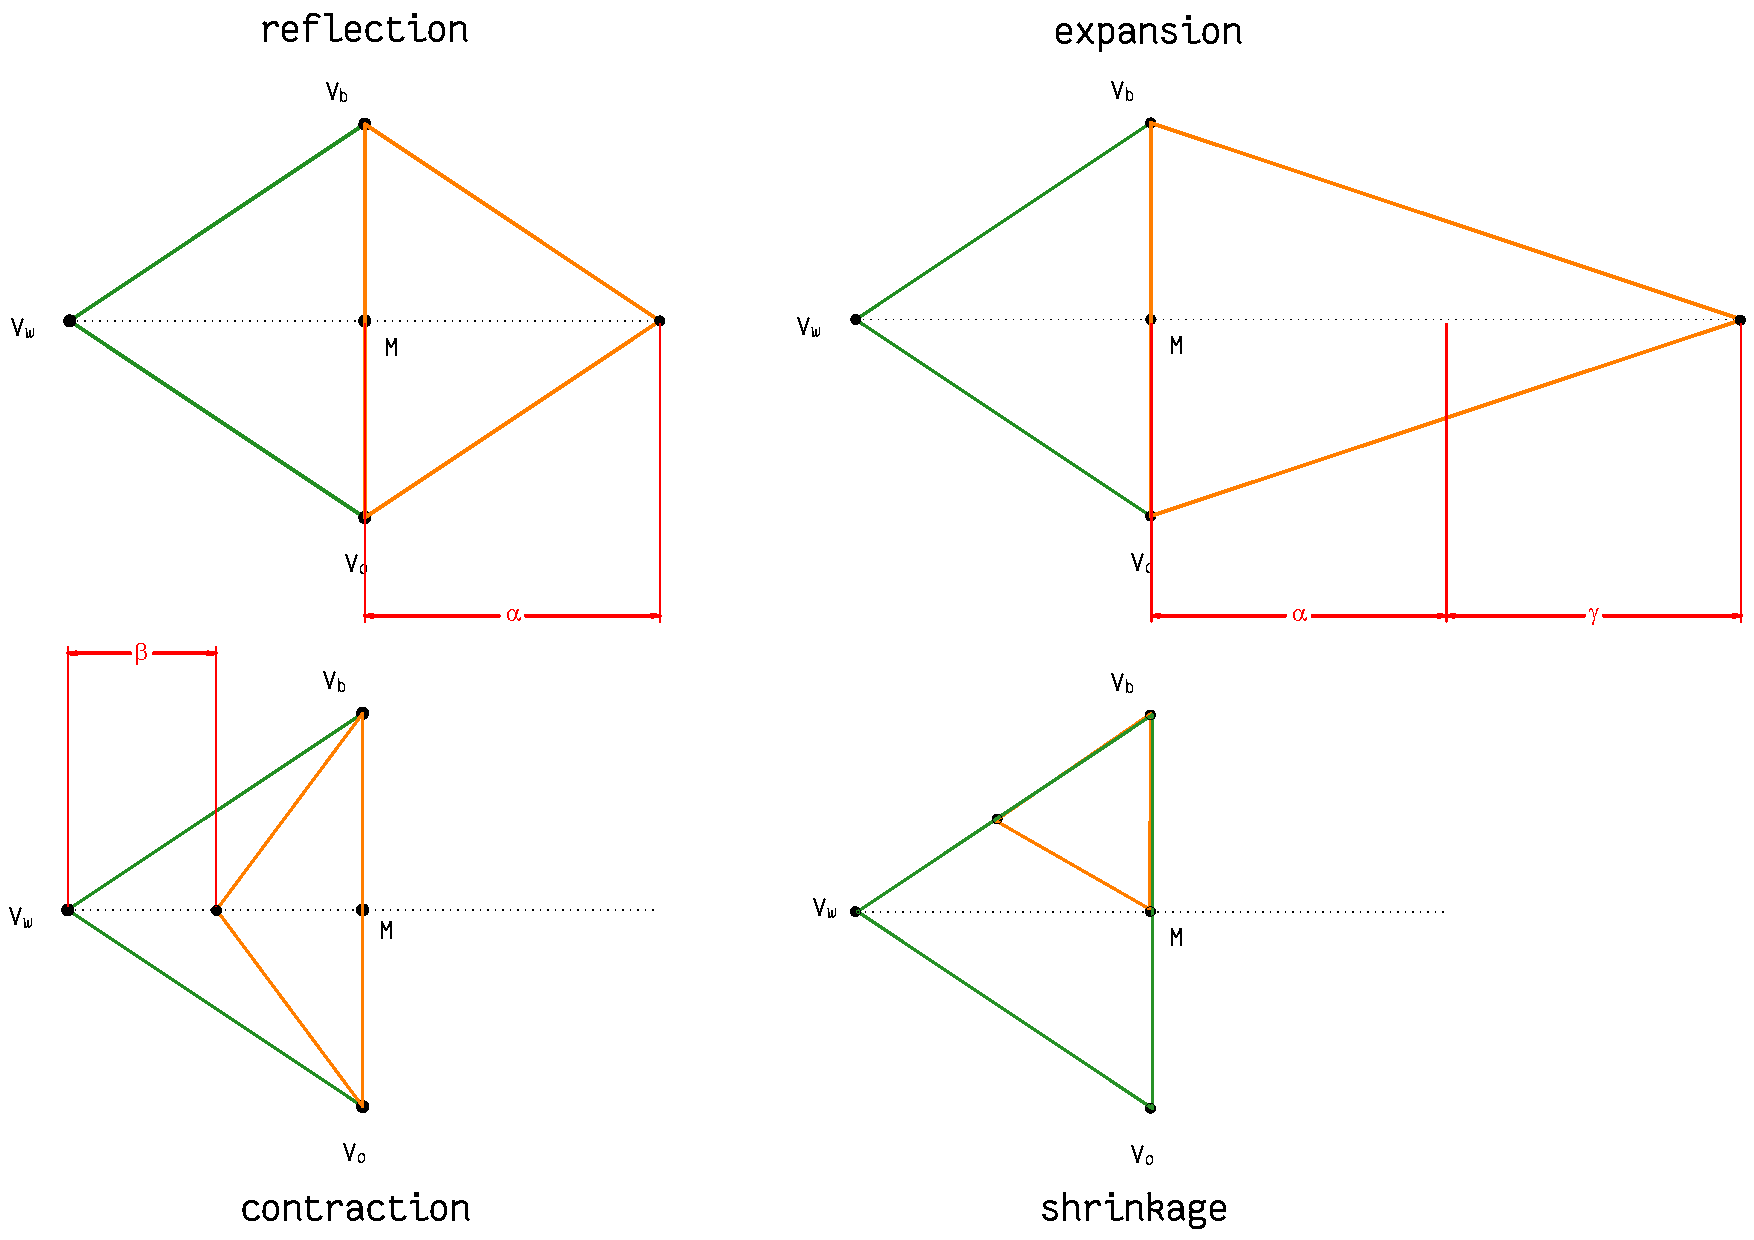
\includegraphics[width=\textwidth]{Graphics/Simplex-moves}
\end{figure}

A simplex is a geometric figure that has one more vertex than the space in which it lives has dimensions. The \skalar{p} Parameters of a fitting problem define a \skalar{p}-dimensional space, in our example we have two parameters, the space hence is a plane and the simplex is a triangle. With tree parameters, the simplex would be a tetrahedron, \Foreign{etc}. Each vertex is characterised by its parameters and, in addition, by the \acs{RSS} associated with it. We then discard the vertex with the highest \acs{RSS}, replacing it with another one with (hopefully) lower \acs{RSS}, so that the vertex ``moves'' downhill. At each step, a vertex can do one of four things (see also fig. \ref{fig:SimMo}):
\begin{description}
  \item[reflection]{move the worst vertex \(V_w \) along the line that connects it to the midpoint \(M \) of the other vertexes for the distance \(\overline{V_wM} + \alpha \overline{V_wM} \). In other words, with \(\alpha = 1 \) the worst vertex is mirrored on the connection between all other vertexes. The new vertex is accepted, if its \acs{RSS} is neither higher than that of \(V_w \), nor lower than that of the best vertex \(V_b \). }
  \item[contraction]{If the \acs{RSS} of the reflected vertex is worse than \(V_w \), the program tries to move this vertex for only \(\beta \overline{V_wM} \). The new vertex is accepted if its \acs{RSS} is lower than that of \(V_w \).}
  \item[expansion]{If the new vertex is better than the previously best vertex \(V_b \), the program tries to move it even further along the line used for reflection, that is for a total of \(\overline{V_wM} + (\alpha+\gamma)\overline{V_wM} \). This expanded vertex is accepted if its \acs{RSS} is lower than that of the discarded \(V_w \).}
  \item[shrinkage]{If in contraction the \acs{RSS} of the new vertex is lower than that of \(V_w \), the program keeps the best vertex and moves all others toward it by half their distance. }
\end{description}
It was shown in \parencite{Kim-97}, however, that shrinkage can never occur, and hence is redundant. The simplex algorithm is guaranteed never to diverge, it is quite efficient as no matrix operations are required. Round-off errors are minimised, but all calculations should be done at least in double precision, with the old Turbo Pascal \texttt{real}-type the algorithm sometimes did not converge, the simplex continued to rotate around the optimum until the maximal number of iterations was reached. To avoid the simplex to become trapped in a local minimum, the starting estimates should be as close to the final parameters as possible. Alternatively, use several -- wildly different -- starting values and verify that they result in the same final parameters.

Instead of \acs{RSS}, other parameters may also be used to control the fit. For noisy data, the median of residuals is more stable against outlying data points. For data with constant relative (rather than absolute) error, \(\chi^2 \) (the sum of squared relative errors) is the appropriate fitting criterium.

\section{Examples}

\subsection{Enzyme kinetics with [S] spanning several orders of magnitude: heteroscedasticity}

\begin{figure}
 \caption{ATPase-activity of Mdr1 as function of [ATP]. The data can be well described by a model with four catalytic and one inhibitory binding site, this results in a ratio of polynoms of 4/5 grade. However, while points at high [ATP] can be fitted by minimising \(\chi^2 \) or RSS, at low concentrations the data can be fitted only with \(\chi^2 \). The data have equal relative error, at low [ATP] the velocities, and hence absolute errors, are so small that they make negligible contribution to \acs{RSS}.}
 \label{fig:ATPase}
 \centering
 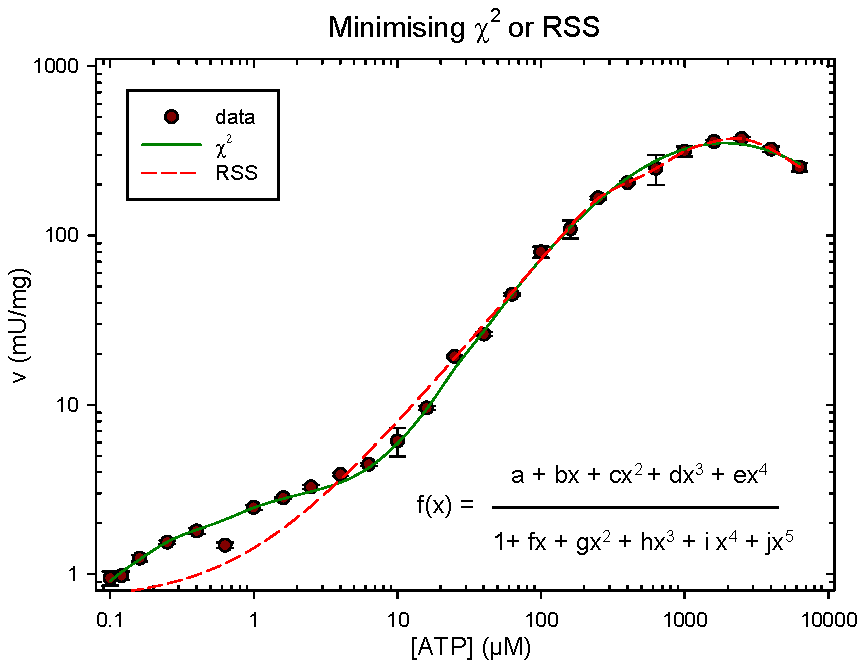
\includegraphics[width=0.75\textwidth]{Graphics/ATPase-chisqr-rss}
\end{figure}

Normally, enzyme kinetics data cover substrate concentrations of two orders of magnitude, between \(0.1 K_m \) and \(10 K_m \). A  minimum of \num{12} data points, equally spaced, in this interval are required for fitting of the \Name{Henri-Michaelis-Menten} (HMM) curve \parencite{Rit-96}. However, some ATPases have several ATP-binding sites with very different \(K_m \). For example, in P-type ATPases like \chemical{Na/K}-ATPase these are \SI{0.1}{\micro M} and \SI{300}{\micro M}, respectively. The question arose, whether ABC-type ATPases like Mdr1, who have two ATP-binding sites in each molecule, would operate with HMM-kinetics, or show cooperativity like the P-type ATPases (where several enzyme molecules with one binding site each have to work together). Therefore, the \( v / [S] \) curve of Mdr1 was measured in the concentration range from \SI{100}{nM} to \SI{10}{mM}, that is, over 5 orders of magnitude \parencite{Bux-99b}. All experiments contained the same amount (\SI{3500}{Bq}) of \textgamma\isotope[33]{P}-ATP as label, but different concentrations of unlabelled ATP, resulting in different specific radioactivity. The formation of \chemical{H}\isotope[33]{P}\chemical{O_4^{2-}} was measured, resulting in velocities that had the same \emph{relative} error. Use of the minimal \acs{RSS} criterion, however, requires data with the same \emph{absolute} error (homoscedasticity). Only minimising \(\chi^2 = \sum_{i=1}^n{\left[\frac{(\hat{\AbsVec{y}}_i - \AbsVec{y}_i)}{\AbsVec{y}_i}\right]^2} \), the sum of squared \emph{relative} errors, allows these data to be fitted, \acs{RSS} fails at low substrate concentrations (see fig. \ref{fig:ATPase}).

\subsection{Fitting of a system of differential equations to a data set}

\begin{figure}
 \caption{System of linear differential equations for the equation A \(\rightarrow \) B \(\rightarrow \) C, the measured values are the intermediate product multiplied by an extraction efficiency (mean and standard deviation of 4 repetitions). For details see text. }
 \label{fig:extract}
 \centering
 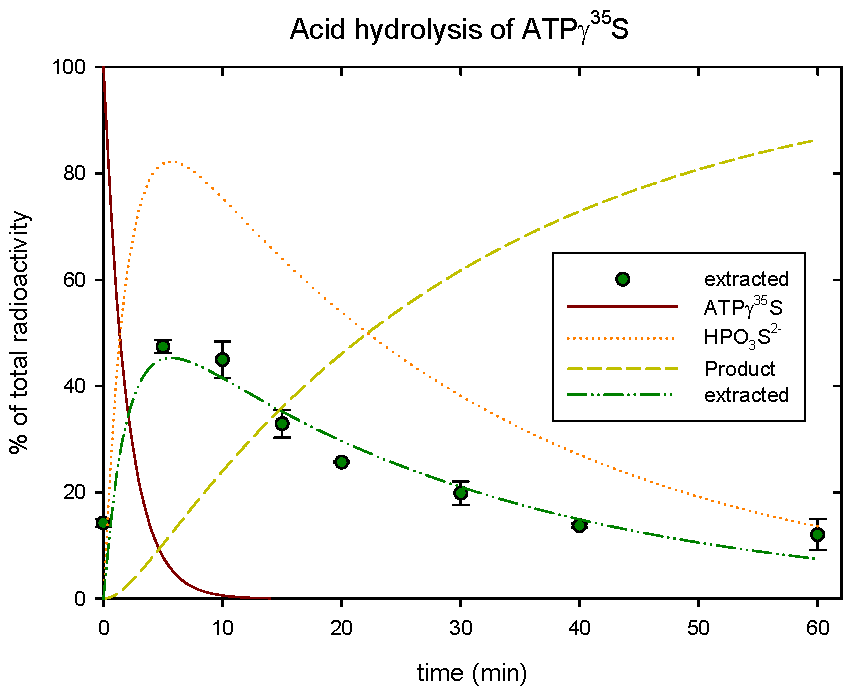
\includegraphics[width=0.75\textwidth]{Graphics/FitSystem}
\end{figure}

The question was whether \SI{70}{kDa} heat shock protein could hydrolyse the ATP-analog ATP\textgamma\isotope[35]{S}. The common method for the determination of \isotope[33]{P}\chemical{O_4^{2-}} is to convert the phosphate to \chemical{(NH_4)_3[P(Mo_3O_{10})_4]} in the presence of carrier phosphate and to extract into organic solvent, the radioactivity in that extract is then counted. To determine whether this method could also be used for thiophosphate, a small amount of ATP\textgamma\isotope[35]{S} was hydrolysed in \SI{2}{N} \chemical{H_2SO_4} at \SI{95}{\celsius}, and samples taken at several time points. Under these conditions, ATP and similar high-energy compounds are hydrolysed quantitatively within \SI{7}{min}. However, it turned out that the thiophosphate is destroyed by the boiling sulphuric acid. Thus, we have a system\\
   ATP\textgamma\isotope[35]{S} \(\autorightarrow{ \(k_1 \)}{} \)  ADP + \chemical{H_2PO_3}\isotope[35]{S^{-}} \\
   \chemical{H_2PO_3}\isotope[35]{S^{-}} \(\autorightarrow{\( k_2 \)}{} \)  non-extractable Product\\
giving a first-order system of coupled linear differential equations
\begin{equation}
  \left\{
  \begin{array}{r@{\;}c@{\;}l}
     \frac{dA}{dt} &=& -k_1 A,\quad A_0 = \SI{100}{\%} \\
     \frac{dB}{dt} &=& k_1 A - k_2 B,\quad B_0 = \SI{0}{\%} \\
     \frac{dC}{dt} &=& k_2 B,\quad C_0 = \SI{0}{\%}
  \end{array}
  \right.
\end{equation}
The reaction was simulated as a system of coupled differential expression with a DP5(4)T4 \Name{Runge-Kutta}-algorithm \parencite{Hei-92} with the parameters \(k_1, k_2 \) and extraction efficiency, the independent variable time and the dependent variable radioactivity extracted. Fitting was performed by simplex with \acs{RSS} as criterium. The best fit was obtained with \(k_1 = \SI{0.509}{min^{-1}},\ k_2 = \SI{0.034}{min^{-1}} \) and an extraction efficiency of \SI{55.1}{\%} (see fig. \ref{fig:extract}). The extraction method is therefore suitable for the determination of thiophosphate, if the relatively low extraction efficiency is taken into account.

This example shows the incredible flexibility of the simplex algorithm even for very unusual fitting problems.

\section{Error estimation}

\subsection{Confidence intervals for parameters}

When the noise in the data is normally distributed with constant variance, all information about the parameter vector \skalar{\beta} is in the \(\mathrm{RSS}(\beta) = \sum_{i=1}^n{[\AbsVec{y}_i - f(\arr{X}_{i\cdot},\beta)]}\) \parencite{Wat-94}. The parameter inference region for the interference interval \((1-\alpha)\) is an ellipsoid given by \(\mathrm{RSS}(\beta) = \mathrm{RSS}_F\) with
\begin{equation}
  \mathrm{RSS}_F = \mathrm{RSS}(\hat{\beta})\left[1 + \frac{p}{n-p} F(p, n-p, \alpha)\right]
\end{equation}
Alternatively, \(\mathrm{RSS}(\beta) = \mathrm{RSS}_t\) can be used with
\begin{equation}
  \mathrm{RSS}_t = \mathrm{RSS}(\hat{\beta})\left[1 + \frac{t^2(n-p, \alpha/2)}{n-p}\right]
\end{equation}
Thus, we can profile the \acs{RSS} surface as follows:
\begin{enumerate}
  \item{Out of the \skalar{p} parameters, select \(\beta_j\) and the increment \( \Delta = 0.1 \times \mathrm{se}(\hat{\beta}_j) \).}
  \item{Initialise \( \beta_j = \hat{\beta}_j \) and \( \tilde{\beta}(\beta_j) = \hat{\beta} \).}
  \item{Increment \( \beta_j \leftarrow \beta_j + \Delta \) and use previous \( \tilde{\beta}(\beta_j) \) as starting value. Converge to \( \tilde{\beta}(\beta_j) \) the profile \acs{RSS}. Store \( \beta_j, \tilde{\beta}(\beta_j), \widetilde{\mathrm{RSS}}(\beta_j) \). }
  \item{Repeat (3) as necessary.}
  \item{Set \( \Delta = -\Delta \) and go to (2) to profile \( \beta_j < \hat{\beta}_j \). }
  \item{When enough information has been obtained on \skalar{\beta_j} to estimate its confidence interval, increment \skalar{j} and go to (1).}
\end{enumerate}

We want for all parameters to find those values of \skalar{\beta_p} where \( \mathrm{RSS}(\beta_j) = \mathrm{RSS}_t \). We could do that by plotting \( \mathrm{RSS}(\beta_j) \) against \( \beta_j \), or, alternatively, by
\begin{enumerate}
  \item{Calculate \Name{Student}ised parameters \( \delta(\beta_j) = \frac{(\beta_j - \hat{\beta}_j)}{\mathrm{se}(\beta_j)} \).}
  \item{Convert the profile \acs{RSS} to corresponding profile \skalar{t}-values by \( t(\beta_j) = \sgn(\beta_j - \hat{\beta}_j) \sqrt{\frac{\widetilde{\mathrm{RSS}}(\beta_j) - \mathrm{RSS}(\hat{\beta})}{s^2}} \).}
  \item{Plot \skalar{t(\beta_j)} against \skalar{\delta(\beta_j)}.}
  \item{The points defining a \skalar{1 - \alpha} marginal interval correspond to the points where \( t(\beta_j) = \pm t(n-p, \alpha/2) \). This are the intersections of the \skalar{t(\beta_j)} against \skalar{\delta(\beta_j)} curve with the lines \skalar{\pm t(n-p, \alpha/2)}. }
  \item{Convert the \skalar{\delta}- into \skalar{\beta}-values. }
\end{enumerate}
The conversion to \Name{Student}ised parameters makes comparison between the parameters within the model and across different models (with a different number of parameters) easier. If the model is linear in the parameters, the profile \skalar{t} plot would be a line through the origin with slope \num{1}. One can also plot the trace vector \skalar{\tilde{\beta}(\beta_j)} against the profile parameter \skalar{\beta_j}, in linear models this results in a straight line with slope the correlation \skalar{r} between the parameters, in non-linear models we get curves.

\subsubsection{Monte Carlo methods}

This method \parencite{Str-92, Str-10} is computationally expensive. It consists of the following steps:
\begin{enumerate}
  \item{Determine the most probable parameters }
  \item{Calculate \skalar{\hat{\AbsVec{y}}} from this model and treat this vector as ``perfect'' }
  \item{Generate synthetic data by adding pseudo-random noise to \skalar{\hat{\AbsVec{y}}}, repeat \num{e2}--\num{e3} times.  }
  \item{Determine and tabulate the most likely parameters of these simulated data sets }
  \item{Generate a histogram of the distribution of the simulated parameters }
\end{enumerate}
The distribution of the noise should be identical to the standard deviation of the experimental data. Alternatively, one can use the residuals from step 1, reshuffling them between the data points. This does not make any assumptions about the error distribution of the data points.


\subsection{Goodness of fit}

If the function used for fitting is appropriate for the data, the residuals \( r_i = \AbsVec{y}_i - \hat{\AbsVec{y}}_i \) should have a random, \Name{Gauss}ian distribution. This can be tested in various ways.

\subsubsection{The runs test}

The runs test quantifies trends in residuals. If the residuals are distributed randomly, the probability of a residual \skalar{r_i} to be positive or negative is independent of the previous \skalar{r_{i-1}} and following \skalar{r_{i+1}} residual. If, however, there is a systematic deviation between the data and the model, clusters of positive and negative residuals will occur. A \textbf{run} is a  group of consecutive residuals with the same sign. Trends will reduce the number of runs, serial correlations will increase it. The expected number of runs \skalar{R_e} can be calculated from the total number of positive (\skalar{n_+}) and negative residuals (\skalar{n_-}) as \( R_e = \frac{2 n_+ n_-}{n_+ + n_-} + 1 \), with a variance of \( \sigma^2_R = \frac{2n_+ n_- (2n_+ n_- - n_+ - n_-)}{(n_+ + n_-)^2 (n_+ + n_- -1)} \). We then compare the observed number of runs (\skalar{R_o}) with the expected by calculating a test statistics \( Z = |\frac{R_o - R_e \pm 0.5}{\sigma_r}| \), which with \skalar{n_+} and \skalar{n_-} both \(> 10 \) will be distributed approximately as a standard normal variable, that is, \skalar{Z} is the number of standard deviations that \skalar{R_e} and \skalar{R_o} are apart. The value of \(\pm\)\num{0.5} is a continuity correction to account for biases introduced by approximating a discrete distribution with a continuous one, it is positive when testing for to few runs, and negative when testing for too many runs. Usually, a value of \( Z \geq 1.65 \rightarrow\  P_0 < \SI{5}{\%} \) is reason for concern.

Serial correlation can be formally detected by the \Name{Durbin-Watson} test, or operationally by plotting all residuals \skalar{r_i} against the residual \skalar{r_{i+j}} \skalar{j} data points away from it (lag\textsubscript{j}-plot). Usually, the correlation is strongest with small \skalar{j} and vanishes as \skalar{j} is increased.

\subsubsection{\skalar{F}-test}

The runs-test described above is a non-parametric test, it is easy to apply but the sensitivity (ability to detect significant deviations) is lower than that of appropriate parametric tests. \parencite[pp. 286--290]{Kre-79} describes such a test with \skalar{H_0}: the residuals can be explained by the standard deviation of the data points, \Foreign{versus} \skalar{H_1}: the residuals are larger than expected given the standard deviation of the data points. The sensitivity of this test is paid for by its laborious nature.

The \skalar{n} data points occur in \skalar{r} different values for \AbsVec{x}, so that \( n_1 + n_2 + \ldots + n_r = n \). For each distinct \( \AbsVec{x}_i \), we can define the \AbsVec{y}-average \( \bar{\AbsVec{y}}_i \), and we can also define the total average \( \bar{\AbsVec{y}} \). Then \( q  = q_1 + q_2 = \sum_{i=1}^r{\sum_{j=1}^{n_i}{(\AbsVec{y}_{ij} - \hat{y}_i)^2}} \) can be resolved into two components, \( q_1 = \sum_{i=1}^r{n_i (\bar{\AbsVec{y}}_i - \hat{\AbsVec{y}}_i)^2} \) describes the scatter of the group means around the regression curve with \( \nu_1 = r - p \) degrees of freedom and \( q_2 = \sum_{i=1}^r{\sum_{j=1}^{n_i}{(\AbsVec{y}_{ij} - \bar{\AbsVec{y}}_i)^2}} \) the scatter within the groups with \(\nu_2 = n - r \) degrees of freedom, \( \nu_q = n - p\). Then \( v_0 = \frac{q_1/\nu_1}{q_2/\nu_2} \) is randomly distributed with \skalar{F(\nu_1, \nu_2)}, and we look for \( (P(v_0 \leq c) = 1 - \alpha\), where \skalar{\alpha} is the desired level of significance (say, \SI{5}{\%}). If \( v_0 \leq c \) we accept the regression curve as a valid representation of the data, otherwise, we need to look for a better regression equation.

\paragraph{Example}

\begin{figure}
 \caption{ATPase activity of Mdr1: Number of kinetically different sites. For details see text. }
 \label{fig:ATPsites}
 \centering
 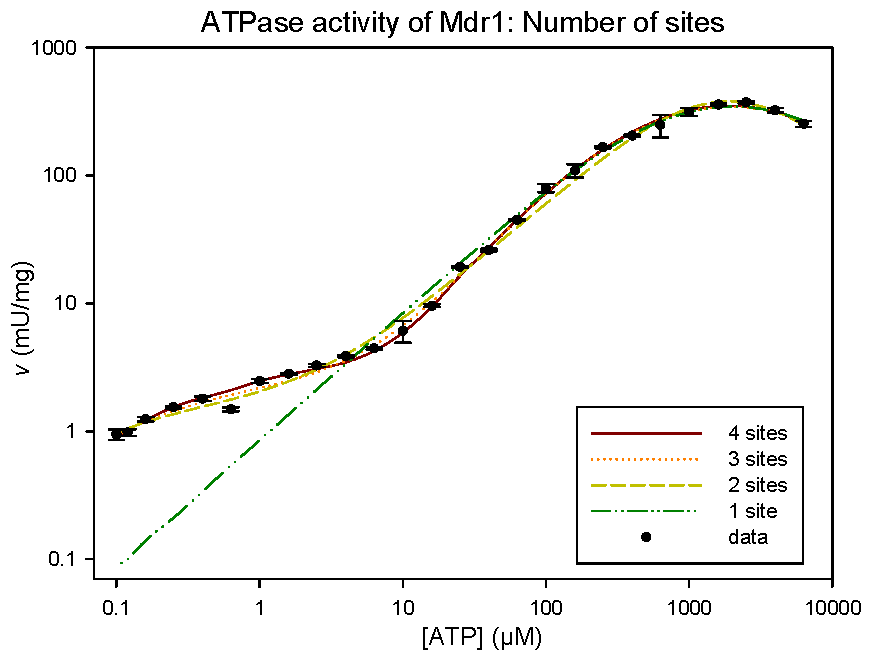
\includegraphics[width=\textwidth]{Graphics/ATPase-sites}
\end{figure}

To determine the number of ATP-binding sites in Mdr1 the substrat/velocity curve was measured (see fig. \ref{fig:ATPsites}). As shown already in  fig. \ref{fig:ATPase}, these data cannot be fitted by the least squares criterium, but the \(\chi^2\)-criterium works very well. Relative errors were used throughout the analysis. Increasing the number of sites (and hence the order of the ratio of polynoms) results in more flexible curves, and hence a better fit to the data. However, this may be caused by a fit to the noise (overfitting). Results for models with 1--4 catalytic binding sites, plus a site for substrate inhibition are summarised in this table, \( \nu_1 = 24,\quad \nu_2 = 212,\quad q_2 = 2079.4 \):

\begin{tabular}{rrrrr}
  \toprule
               & 1 site         & 2 sites             & 3 sites        & 4 sites      \\
  \midrule

  \skalar{q_1} & \num{54762.6}  & \num{3894.0}        & \num{2290.1}   & \num{603.2}  \\
  F            & \num{232.6}    & \num{16.5}          & \num{9.73}     & \num{1.56}   \\
  P(0) \%      & \(<0.1\)       & \(<0.1\)            & \(<0.1\)       & \num{5.2}    \\
 \bottomrule
\end{tabular}

The \(F\)-test shows that curves for 1--3 catalytic binding sites do not explain the data well, we can reject \skalar{H_0} (the residuals can be explained by the standard deviation of the data) with an error probability of less than \SI{0.1}{\%}. For a model with 4 catalytic sites, on the other hand, the null-hypothesis is accepted at the \SI{5}{\%} level. Thus, Mdr1 must have at least four kinetically different binding sites for ATP. We cannot be sure wether it is only four sites or even more; but we can exclude models with fewer sites.

For the runs test the one-site model gives us \(+-----++-+-++++++----------\), the two-site model  \(---+++-------++++---+--+-\), the three-site model  \(+---+++-+--+-+++----+---+-\) and four-site model \(+---+++-+-++--------+++++-\). Thus, we get

\begin{tabular}{rrrrr}
  \toprule
                &  1    &  2    &  3    &   4    \\
  \midrule
  \(n_+\)       & 10    &  9    & 11    &  12    \\
  \(n_-\)       & 16    & 17    & 15    &  14    \\
  \(n\)         & 26    & 26    & 26    &  26    \\
  \(R_o\)       &  9    &  9    & 14    &  10    \\
  \(R_e\)       & 13.3  & 12.8  & 13.7  &  11.9  \\
  \(\sigma_R\)  &  1.42 &  5.07 &  5.94 &   6.16 \\
  \(Z\)         &  2.68 &  0.64 &  0.16 &   0.23 \\
  \bottomrule
  \(P_0\) \si{\%}& 0.37 & 25.1  & 43.6  &  40.9  \\
  \bottomrule
\end{tabular}

In other words, we can reject the one-site model (even if not at the same high confidence as with the \(F\)-test), but we cannot see a significant improvement beyond the 2-site model. This lower sensitivity of the runs test is typical for non-parametric compared to parametric tests. On the other hand, non-parametric tests are a lot less work!

\section{Code for Simplex-Regression}

The following program was modified from \parencite{Nel-65,Cac-84}. The formula compiler was published in \parencite{Gie-87b}, error limit determination by Monte-Carlo simulation was described in \parencite{Str-92}.

\begin{lstlisting}[caption=Simplex]
  UNIT SimplexFit;

  {Regressionsanalyse nach M.Caceci, W.P. Cacheris: Fitting Curves to Data,
        Byte Magazine May 1984, S. 340-350
   Unter Benutzung des Formel-Compilers aus Pascal International 8/1987, S. 52-60
   Die Bestimmung der Fehlergrenzen durch Monte-Carlo-Simulation ist beschrieben
        von Straume & Johnson, Meth. Enzymol. 210 (1992) 117-129
   Die Idee der Minimierung von Chi2 für Daten mit bekannten Fehlergrenzen stammt
        aus Press et al.: Numerical Recepies in Pascal, Cambridge 1989
   Gesamtprogramm copyright 1988-1994 by Dr. Engelbert Buxbaum }

  INTERFACE

  USES MathFunc,            // basic maths
       crt,                 // low level system calls
       Calc,                // formula compiler
       Vector,              // vector arithmetic
       Matrix,              // matrix arithmetic
       Deskript,            // descriptive statistics
       Zufall               // random numbers
       ;

  CONST
    SimplexError: BOOLEAN = FALSE;

  PROCEDURE Approximation(Data: MatrixTyp; VAR yBerech: VectorTyp;
    VAR ProblemName, Formel, xName, yName: STRING);


  IMPLEMENTATION

  CONST
    alfa                  = 1.0;                 // Reflektion coefficient
    beta                  = 0.5;                 // Kontraktion coefficient
    gamma                 = 2.0;                 // Expansion coefficient
    MaxParameter          = 10;
    MaxVariablen          = 10;
    MaxN                  = MaxParameter + 1;    // dimension of simplex
    lw                    = 5;                   // linewidth of data field + 1
    Page                  = 12;
    Ja                    = 'Y';                 // key for yes
    Nein                  = 'N';                 // key for no

  var ch : char;                                     // for error handling

  PROCEDURE Approximation(Data: MatrixTyp; VAR yBerech: VectorTyp;
    VAR ProblemName, Formel, xName, yName: STRING);

  TYPE
    AVektor = ARRAY[1..MaxN] OF float;
    DataRow = ARRAY [1..MaxVariablen] OF float;
    simpl   = ARRAY [1..MaxN] OF AVektor;            // Simplex
    ParFeld = ARRAY [1..MaxParameter] OF STRING[10];
    VarFeld = ARRAY [1..MaxVariablen] OF STRING[10];

  VAR
    FehlerGrenzen,                    // Letzte Spalte der Daten-Matrix Fehlergrenzen?
    done: BOOLEAN;                    // Konvergenz

    i, j, n: BYTE;

    h, l: ARRAY [1..MaxN] OF BYTE;    // Zahl Hoch/Niedrig Parameter

    Daten,                            // Zahl der Datenpunkte
    MaxIter,                          // max.Zahl der Iterationen
    NIter: WORD;                      // Zahl der Iterationen

    Next,                             // neuer Vertex zu testen
    center,                           // Minimum aller Vertexe}
    mean, error, MaxErr,              // Maximal zulaessiger Fehler}
    p, q,                             // um ersten Simplex zu berechnen
    step: AVektor;                    // Eingabe Startschritte

    simp: simpl;                      // Simplex

    NameA,                            // Name des Eingabefiles
    NameB: STRING[64];                // Name des Ausgabefiles

    Eindat,                           // Eingabefile
    Ausdat: TEXT;                     // Ausgabefile}

    x: Calc_VarTab;                   // FOR formula compiler
    dummy, Sigma: float;              // y-Standardabweichung
    Formula: Calc_String;
    FormProg: Calc_Prog;

    Variablen, Parameter: BYTE;

    ErrorStat,                        // TRUE wenn Fehlerstatistik gewuenscht
    Erster: BOOLEAN;                  // Startsimplex nur einmal ausgeben

    Antwort: CHAR;

    Methode: (Summe, Median, ChiSqr);  // was soll minimiert werden?


    {****************************************************************************}

    PROCEDURE LiesFunction(VAR x: Calc_VarTab; VAR Formula: Calc_String;
    VAR FormProg: Calc_Prog);

    VAR
      i: BYTE;
      dummy: float;
      Name: Calc_IdStr;
      Input : TEXT;


      PROCEDURE Hilfe;

      BEGIN
        Writeln('The function used for fitting to the data should be entered in the ');
        Writeln('following manner: ');
        Writeln('1) Number and names of the variables (i. e. measured data)');
        Writeln('2) Number and name(s) of the parameters');
        Writeln('3) The formula itself. All names must be entered exactly as defined.');
        Writeln('   No undefined names are allowed. The formula must end with a ');
        Writeln('   semicolon.');
        Writeln;
        Writeln('The compiler ''knows'' the following constants and and functions, which ');
        Writeln('can not be redefined:');
        Writeln('Constants: e, pi                        Basic operators: +, -, *, /, ^');
        Writeln('Integer: div, mod, ggt, kgv             Logarithms: ln, lg, ld, exp');
        Writeln('sin, cos, tan, cot and the equivalent hyperbolic and arcus functions');
        Writeln('Various Functions: abs, deg, rad, fak, sgn');
        Writeln;
      END;


    BEGIN
      Hilfe;
      Assign(Input, 'CON');
      Reset(Input);
      IF SimplexError THEN EXIT;
      CalcDecMod := TRUE;                     {nur definierte Vars und Parms}
      x := NewVarTab;
      Writeln('Data file has ', MatrixColumns(Data), 'columns');
      IF MatrixColumns(Data) > 2
        THEN
          BEGIN
            Write('Last column independend variable or error margin (v/e):');
            REPEAT
              Readln(Antwort);
              Antwort := UpCase(Antwort);
            UNTIL (Antwort IN ['V', 'F', 'E', #27]);
            IF Antwort = #27
              THEN
                BEGIN
                  SimplexError := TRUE;
                  EXIT;
                END;
            FehlerGrenzen := (Antwort = 'F') OR (Antwort = 'E');
          END
        ELSE
          FehlerGrenzen := FALSE;
      IF FehlerGrenzen
        THEN Variablen := Pred(MatrixColumns(Data))
        ELSE Variablen := MatrixColumns(Data);
      Daten := MatrixRows(Data);
      FOR i := 1 TO Pred(Variablen) DO
        BEGIN
          Write('Name of the ', i, '. (independent) variable: ');
          Readln(Name);
          dummy := AddToVarTab(x, Name);
        END;
      Write('Name of the ', Variablen, '. (dependent) variable: ');
      Readln(Name);
      dummy := AddToVarTab(x, Name);
      Write('How many parameters do you want to use [1..', MaxParameter, ']: ');
      ReadLn(Parameter);
      N := Parameter + 1;               {Dimensionen des Simplex}
      FOR i := 1 TO Parameter DO
        BEGIN
          Write('Name of the ', i, '. parameter: ');
          ReadLn(Name);
          dummy := AddToVarTab(x, Name);
        END;
      REPEAT
        Writeln('Please enter the equation: ');
        Writeln;
        Write(x^[Variablen].VarId, ' = ');
        ReadLn(Formula);
        CompileExpression(Formula, x, FormProg);
        IF NOT CalcResult
          THEN Writeln('Unable to compile the equation, please try again: ');
      UNTIL CalcResult;
      Formel := x^[Variablen].VarID + ' = ' + Formula;
      xName := x^[1].VarID;
      yName := x^[Variablen].VarID;
    END;


    FUNCTION f(p: AVektor; d: MatrixTyp; Zeile: WORD): float;

    VAR
      i: BYTE;

    BEGIN
      FOR i := 1 TO Variablen DO
        AssignVar(x, x^[i].VarId, GetMatrixElement(d, Zeile, i));
      FOR i := 1 TO Parameter DO
        AssignVar(x, x^[Variablen + i].VarId, p[i]);
      Result := CalcExpression(FormProg, x);
    END;


    PROCEDURE Inparam(VAR MaxIter: WORD; VAR simp: Simpl; VAR Step, MaxErr: AVektor);
    {Einlesen aller benutzerdefinierten Parameter}

    VAR
      FalscheEingabe: BOOLEAN;
      Quelle: CHAR;
      i: WORD;
      c: CHAR;

    BEGIN
      Writeln('This routine calculates curve fits by the simplex algorithm');
      Writeln;
      LiesFunction(x, Formula, FormProg);
      IF SimplexError THEN EXIT;
      REPEAT
        FalscheEingabe := FALSE;
        Writeln;
        Write('Please enter the name of the output file: ');
        ReadLn(NameB);
        Assign(Ausdat, NameB);
        Rewrite(Ausdat);
        IF IOResult <> 2
          THEN   { d. h., Datei existiest schon }
            BEGIN
              REPEAT
                Write(NameB, ' already exists. Overwrite (y/n): ');
                ReadLn(c);
                c := UpCase(c);
              UNTIL (c = JA) OR (c = Nein) OR (c = #27);
            IF (c = #27)
              THEN
                BEGIN
                  SimplexError := TRUE;
                  EXIT;
                END;
            FalscheEingabe := (c = Nein);
          END;
      UNTIL NOT FalscheEingabe;
      Rewrite(Ausdat);
      Write(Ausdat, 'best fit for equation: ');
      Writeln(Ausdat, x^[Variablen].VarId, ' = ', Formula);
      Writeln(Ausdat);
      REPEAT
        FalscheEingabe := FALSE;
        REPEAT
          IF FehlerGrenzen
            THEN Write('Minimise sum of squares, median of squares or Chi2 (S/M/X): ')
            ELSE Write('Minimise sum or median of squares (S/M): ');
          ReadLn(c);
          c := UpCase(c);
          IF NOT ((c = 'S') OR (c = 'M') OR (c = 'X') OR (c = #27))
            THEN
              BEGIN
                Sound(400);
                Delay(50);
                NoSound;
              END;
        UNTIL (c = 'S') OR (c = 'M') OR (c = 'X') OR (c = #27);
        CASE c OF
          'S': BEGIN
                 Methode := Summe;
                 Writeln(Ausdat, 'Minimising sum of squared residuals ');
               END;
          'M': BEGIN
                 Methode := Median;
                 Writeln(Ausdat, 'Minimising median of squared residuals ');
               END;
          'X': BEGIN
                 IF FehlerGrenzen
                   THEN
                     BEGIN
                       Methode := ChiSqr;
                       Writeln(Ausdat, 'Minimizing Chi2');
                     END
                   ELSE
                     BEGIN
                       ch := WriteErrorMessage('Chi2 erfordert Fehlergrenzen in der letzten Daten-Spalte');
                       SimplexError := TRUE;
                       EXIT;
                     END;
               END;
          #27: BEGIN
                 SimplexError := TRUE;
                 EXIT;
               END;
        END; { case }
        Writeln(Ausdat);
        Write(Ausdat, '                            ');
        FOR i := 1 TO Parameter DO
          Write(Ausdat, x^[i + Variablen].VarId,
            ' ': (ValidFigures + 2 - Length(x^[i + Variablen].VarId)));
        CASE Methode OF
          Summe: Writeln(Ausdat, 'sum of squares ');
          Median: Writeln(Ausdat, 'median of squares');
          ChiSqr: Writeln(Ausdat, 'Chi2');
        END;
      UNTIL NOT FalscheEingabe;
      REPEAT
        FalscheEingabe := FALSE;
        Write('Please enter maximal number of iterations: ');
        ReadLn(MaxIter);
      UNTIL NOT FalscheEingabe;
      REPEAT
        FalscheEingabe := FALSE;
        Writeln('Please enter initial guesses for all parameters: ');
        Write(Ausdat, 'Start coordinates:      ');
        FOR i := 1 TO Parameter DO
          BEGIN
            Write(x^[i + Variablen].VarId, ' = ');
            ReadLn(simp[1, i]);
            IF (i MOD lw) = 0 THEN Writeln(Ausdat);
            Write(Ausdat, FloatStr(simp[1, i], ValidFigures), '  ');
          END;
        Writeln(Ausdat);
        Writeln(Ausdat);
      UNTIL NOT FalscheEingabe;
      REPEAT
        FalscheEingabe := FALSE;
        Writeln('Please enter starting step width for all parameters ');
        Writeln('(ca. 1/10 to 1/2 of initial value)');
        Write(Ausdat, 'Starting step width:    ');
        FOR i := 1 TO Parameter DO
          BEGIN
            Write('Step width:     ', x^[i + Variablen].VarId, ' = ');
            ReadLn(step[i]);
            IF (i MOD lw) = 0 THEN Writeln(Ausdat);
            Write(Ausdat, FloatStr(step[i], ValidFigures), '  ');
          END;
        Writeln(Ausdat);
        Writeln(Ausdat);
        Write(Ausdat, 'max. alowable error:    ');
        FOR i := 1 TO n DO
          BEGIN
            MaxErr[i] := MaxError;
            IF (i MOD lw) = 0 THEN Writeln(Ausdat);
            Write(Ausdat, FloatStr(MaxErr[i], ValidFigures), '  ');
          END;
        Writeln(Ausdat);
        Writeln(Ausdat);
      UNTIL NOT FalscheEingabe;
      REPEAT
        Write('Do you want error margins for the parameters (y/n): ');
        ReadLn(c);
        c := UpCase(c);
      UNTIL (c = JA) OR (c = Nein) OR (c = #27);
      IF (c = #27)
        THEN
          BEGIN
            SimplexError := TRUE;
            EXIT;
          END;
      Writeln(UpCase(c));
      ErrorStat := (c = JA);
    END;


    PROCEDURE sum_of_residuals(VAR z: AVektor; Data: MatrixTyp);
    {Berechnet die Summe der Fehlerquadrate}

    VAR
      i: WORD;

    BEGIN
      z[n] := 0.0;
      FOR i := 1 TO Daten DO
        z[n] := z[n] + Sqr(f(z, Data, i) - GetMatrixElement(Data, i, Variablen));
    END;


    PROCEDURE Median_Of_Squares(VAR z: AVektor; Data: MatrixTyp);
    { berechnet den Median der Fehlerquadrate }

    VAR
      i: WORD;
      Residuals: VectorTyp;

    BEGIN
      CreateVector(Residuals, Daten, 0.0);
      FOR i := 1 TO Daten DO
        SetVectorElement(Residuals, i, Sqr(f(z, Data, i) -
          GetMatrixElement(Data, i, Variablen)));
      ShellSort(Residuals);
      z[n] := Quantile(Residuals, 0.5);
      DestroyVector(Residuals);
    END;

    PROCEDURE Chi(VAR z: AVektor; Data: MatrixTyp);
    {Berechnet chi2}

    VAR
      i: WORD;

    BEGIN
      z[n] := 0.0;
      FOR i := 1 TO Daten DO
        z[n] := z[n] + Sqr(f(z, Data, i) - GetMatrixElement(Data, i, Variablen) /
          GetMatrixElement(Data, i, Succ(Variablen)));
    END;


    PROCEDURE report;
    {berichtet Programstatistik}

     VAR
      dy, h, Zaehler, Nenner, Fehler, Mittel, rSqr: float;
      d1, d2: TEXT;
      HilfsStr: STRING[14];
      i, j: WORD;

    BEGIN
      Writeln(Ausdat);
      Writeln(Ausdat, 'Routine was left after ', NIter: 5, ' iterations');
      Writeln(Ausdat);
      Writeln(Ausdat);
      Writeln(Ausdat, 'The final simplex is: ');
      Write(Ausdat, '                        ');
      FOR j := 1 TO n DO
        BEGIN
          FOR i := 1 TO n DO
            BEGIN
              IF (i MOD lw) = 0 THEN
                Writeln(Ausdat);
              Write(Ausdat, FloatStr(simp[j, i], ValidFigures), '  ');
            END;
          Writeln(Ausdat);
          Write(Ausdat, '                        ');
        END;
      Writeln(Ausdat);
      Write(Ausdat, 'The mean is:            ');
      FOR i := 1 TO n DO
        BEGIN
          IF (i MOD lw) = 0 THEN
            Writeln(Ausdat);
          Write(Ausdat, FloatStr(mean[i], ValidFigures), '  ');
        END;
      Writeln(Ausdat);
      Writeln(Ausdat);
      Write(Ausdat, 'error:                  ');
      FOR i := 1 TO n DO
        BEGIN
          IF (i MOD lw) = 0 THEN
            Writeln(Ausdat);
          Write(Ausdat, FloatStr(error[i], ValidFigures), '  ');
        END;
      Writeln(Ausdat);
      Writeln(Ausdat);
      Write(Ausdat, '  #    ');
      FOR i := 1 TO Variablen DO
        Write(Ausdat, x^[i].VarId, ' ': (ValidFigures + 2 - Length(x^[i].VarId)));
      IF Fehlergrenzen THEN
        Write(Ausdat, 'Delta ', x^[Variablen].VarId, ' ': (ValidFigures -
          2 - Length(x^[i].VarId)));
      Write(Ausdat, x^[Variablen].VarId, ' ber.',
        ' ': (ValidFigures - 2 - Length(x^[Variablen].VarId)));
      Writeln(Ausdat, 'error:                  ');
      Zaehler := 0;
      sigma := 0.0;
      FOR i := 1 TO Daten DO
        BEGIN
          h := f(mean, Data, i);
          SetVectorElement(yBerech, i, h);
          dy := GetMatrixElement(Data, i, Variablen) - h;
          sigma := sigma + Sqr(dy);
          Write(Ausdat, i: 4, '  ');
          FOR j := 1 TO MatrixColumns(Data) DO
            Write(Ausdat, FloatStr(GetMatrixElement(Data, i, j), ValidFigures), '  ');
          Writeln(Ausdat, FloatStr(h, ValidFigures), '  ', FloatStr(dy, ValidFigures));
          Zaehler := Zaehler + GetMatrixElement(Data, i, Variablen);
        END;
      Writeln(Ausdat);
      sigma := Sqrt(sigma / Daten);
      Writeln(Ausdat, 'The standard deviation is:    ', FloatStr(sigma, ValidFigures));
      Fehler := sigma / Sqrt(Daten - Parameter);
      Writeln(Ausdat, 'The error of the function is: ', FloatStr(Fehler, ValidFigures));
      Mittel := Zaehler / Daten;
      Zaehler := 0;
      Nenner := 0;
      FOR i := 1 TO Daten DO
        BEGIN
          Zaehler := Zaehler + Sqr(GetVectorElement(yBerech, i) - Mittel);
          Nenner := Nenner + Sqr(GetMatrixElement(Data, i, Variablen) - Mittel);
        END;
      rSqr := Zaehler / Nenner;
      Writeln(Ausdat, 'r2:                           ', FloatStr(rSqr, ValidFigures));
    END;


    PROCEDURE First;

    VAR
      i, j: WORD;

    BEGIN
      Write(Ausdat, 'Start simplex ');
      FOR j := 1 TO n DO
        BEGIN
          Write(Ausdat, ' simp[', j: 3, ']');
          FOR i := 1 TO n DO
            BEGIN
              IF (i MOD lw) = 0 THEN Writeln(Ausdat);
              Write(Ausdat, FloatStr(simp[j, i], ValidFigures), '  ');
            END;
          Writeln(Ausdat);
          Write(Ausdat, '              ');
        END;
      Writeln(Ausdat);
    END;


    PROCEDURE new_vertex;
    {ersetzt worst durch next}

    VAR
      i, j: WORD;

    BEGIN
      IF erster THEN Write(' --- ', NIter: 4);
      FOR i := 1 TO n DO
        BEGIN
          simp[h[n], i] := Next[i];
          IF erster THEN Write(FloatStr(Next[i], ValidFigures));
        END;
      IF erster THEN Writeln;
    END;


    PROCEDURE order;
    {Highs und Lows fuer jeden Parameter}

    VAR
      i, j: BYTE;

    BEGIN
      FOR j := 1 TO n DO
        BEGIN
          FOR i := 1 TO n DO
            BEGIN
              IF simp[i, j] < simp[l[j], j] THEN l[j] := i;
              IF simp[i, j] > simp[h[j], j] THEN h[j] := i;
            END;
        END;
    END;


    PROCEDURE Iteration(Data: MatrixTyp);

    VAR
      i, j: WORD;

    BEGIN
      NIter := 0;
      REPEAT
        done := TRUE;
        NIter := Succ(NIter);
        FOR i := 1 TO n DO center[i] := 0.0;
        FOR i := 1 TO n DO
          IF i <> h[n]
            THEN
              FOR j := 1 TO Parameter DO
                center[j] := center[j] + simp[i, j];
        FOR i := 1 TO n DO
          BEGIN
            center[i] := center[i] / Parameter;
            Next[i] := (1.0 + alfa) * center[i] - alfa * simp[h[n], i];
          END;
        CASE Methode OF
          Summe: sum_of_residuals(Next, Data);
          Median: Median_Of_Squares(Next, Data);
          ChiSqr: Chi(Next, Data);
        END;
        IF Next[n] <= simp[l[n], n]
          THEN
            BEGIN
              new_vertex;
              FOR i := 1 TO n DO
                Next[i] := gamma * simp[h[n], i] + (1.0 - gamma) * center[i];
              CASE Methode OF
                Summe: sum_of_residuals(Next, Data);
                Median: Median_Of_Squares(Next, Data);
                ChiSqr: Chi(Next, Data);
              END;
              IF Next[n] <= simp[l[n], n] THEN new_vertex;
            END
          ELSE
            BEGIN
              IF Next[n] <= simp[h[n], n]
                THEN
                  new_vertex
                ELSE
                  BEGIN
                    FOR i := 1 TO Parameter DO
                      Next[i] := beta * simp[h[n], i] + (1.0 - beta) * center[i];
                    CASE Methode OF
                      Summe: sum_of_residuals(Next, Data);
                      Median: Median_Of_Squares(Next, Data);
                      ChiSqr: Chi(Next, Data);
                    END;
                    IF Next[n] <= simp[h[n], n]
                      THEN
                        new_vertex
                      ELSE
                        BEGIN
                          FOR j := 1 TO Parameter DO
                            BEGIN
                              simp[i, j] := (simp[i, j] + simp[l[n], j]) * beta;
                              CASE Methode OF
                                Summe: sum_of_residuals(simp[i], Data);
                                Median: Median_Of_Squares(simp[i], Data);
                                ChiSqr: Chi(simp[i], Data);
                              END; // case
                            END; // for j
                        END; // else
                  END; // else
            END; //else
        order;
        FOR j := 1 TO n DO
          BEGIN
            error[j] := (simp[h[j], j] - simp[l[j], j]) / simp[h[j], j];
            IF done
              THEN IF error[j] > MaxErr[j]
                     THEN done := FALSE;
          END;
      UNTIL (done OR (NIter = MaxIter));
    END;


    PROCEDURE DoIteration(VAR Simp: Simpl; Data: MatrixTyp; VAR Mean: AVektor);

    VAR
      i, j: WORD;

    BEGIN
      CASE Methode OF
        Summe: sum_of_residuals(simp[1], Data);
        Median: Median_Of_Squares(simp[1], Data);
        ChiSqr: Chi(simp[1], Data);
      END;
      FOR i := 1 TO Parameter DO
        BEGIN
          p[i] := step[i] * (Sqrt(n) + Parameter - 1) / (Parameter * Sqrt(2));
          q[i] := step[i] * (Sqrt(n) - 1) / (Parameter * Sqrt(2));
        END;
      FOR i := 2 TO n DO
        BEGIN
          FOR j := 1 TO Parameter DO simp[i, j] := simp[1, j] + q[j];
          simp[i, i - 1] := simp[1, i - 1] + p[i - 1];
          CASE Methode OF
            Summe: sum_of_residuals(simp[i], Data);
            Median: Median_Of_Squares(simp[i], Data);
            ChiSqr: Chi(simp[i], Data);
          END;
        END;
      FOR i := 1 TO n DO
        BEGIN
          l[i] := 1;
          h[i] := 1;
        END;
      order;
      IF Erster THEN First;
      Iteration(Data);
      FOR i := 1 TO n DO
        BEGIN
          mean[i] := 0.0;
          FOR j := 1 TO n DO
            mean[i] := mean[i] + simp[j, i];
          mean[i] := mean[i] / n;
        END;
    END;


    PROCEDURE CalculateErrorMargins;

    CONST
      Anzahl = 100;

    VAR
      Counter, Differenz, Ergebniss: AVektor;
      SimulatedData, Ergebnisse: MatrixTyp;
      i, j, k: WORD;


      PROCEDURE Simulate(VAR SimulatedData: MatrixTyp; yBerech: VectorTyp;
        Sigma: float);

      VAR
        i: WORD;
        Wert: float;

      BEGIN
        FOR i := 1 TO MatrixColumns(SimulatedData) DO
          BEGIN
            Wert := RandomLaplace(GetVectorElement(yBerech, i), Sigma);
            SetMatrixElement(SimulatedData, i, Variablen, Wert);
          END;
      END;

    BEGIN
      Sigma := Sqr(Sigma);
      CopyMatrix(Data, SimulatedData);
      CreateMatrix(Ergebnisse, Anzahl, N, 0.0);
      FOR j := 1 TO N DO
        Counter[j] := 0.0;
      FOR i := 1 TO 100 DO
        BEGIN
          Write(i: 3, '  ');
          Simulate(SimulatedData, yBerech, Sigma);
          DoIteration(Simp, SimulatedData, Ergebniss);
          FOR j := 1 TO N DO
            BEGIN
              SetMatrixElement(Ergebnisse, i, j, Ergebniss[j]);
              Counter[j] := Counter[j] + Ergebniss[j];
              Write(FloatStr(Ergebniss[j], ValidFigures), '  ');
            END;
          Writeln;
        END;
      DestroyMatrix(SimulatedData);
      FOR j := 1 TO N DO
        BEGIN
          Counter[j] := Counter[j] / Anzahl;       { Mittelwerte der Parameter }
          Differenz[j] := 0.0;
        END;
      FOR i := 1 TO Anzahl DO
        FOR j := 1 TO N DO
          Differenz[j] := Sqr(Counter[j] - GetMatrixElement(Ergebnisse, i, j));
      Writeln(Ausdat);
      Writeln(Ausdat, 'Standard deviation of the parameters: ');
      Write(Ausdat, '                        ');
      FOR j := 1 TO N DO
        BEGIN
          Differenz[j] := Sqrt(Differenz[j] / Pred(Anzahl));
          IF (j MOD lw) = 0 THEN Writeln(Ausdat);
          Write(Ausdat, FloatStr(Sqrt(Differenz[j]), ValidFigures), '  ');
        END;
      Writeln(Ausdat);
    END;

  BEGIN {Approximation}
    Erster := TRUE;
    Inparam(MaxIter, simp, step, MaxErr);
    IF SimplexError THEN EXIT;
    DoIteration(Simp, Data, Mean);
    CreateVector(yBerech, Daten, 0.0);
    report;
    Erster := FALSE;
    IF ErrorStat THEN CalculateErrorMargins;
    Close(Ausdat);
  END;

  END.
\end{lstlisting}

\begin{lstlisting}[caption=Test program]
  program Simplex;


  USES
    MathFunc,            // basic math functions
    Vector,              // vector arithmetic
    Matrix,              // matrix arithmetic
    Zufall,              // random numbers
    SimplexFit           // curve fit by simplex
    ;

  const MaxData = 100;

  VAR Data                              : MatrixTyp;
      Calculated                        : VectorTyp;
      ProblemName, Formel, xName, yName : STRING;

  { *********************************************************************** }

  PROCEDURE CreateDataSet (VAR Data : MatrixTyp);

  VAR i : WORD;
      x, y : float;

  BEGIN
    FOR i := 1 TO MatrixRows(Data) DO
      BEGIN
        x := i/10 ;
        SetMatrixElement(Data, i, 1, x);
        y := x / (1+x);                  // normalised Henri-Michaelis-Menten law
        y := y + RandomNormal(0, 0.1);   // add normal-distributed random noise
        SetMatrixElement(Data, i, 2, y);
      END;
  END;


  BEGIN {Hauptprogram}
    CreateMatrix(Data, MaxData, 2, 0.0);
    CreateVector(Calculated, MaxData, 0.0);
    CreateDataSet(Data);
    Approximation(Data, Calculated, ProblemName, Formel, xName, yName);
    DestroyMatrix(Data);
    DestroyVector(Calculated);
  END.
\end{lstlisting}


\printbibliography[heading=subbibliography]
\end{refsection}

  % -*- TeX:UK -*-
\chapter{Circular data}
\begin{refsection}
\label{text:circular}

\abstract{There are data whose scale is not on a number ray, but on a circle. Examples include angles on the windrose, hour of day and season of year. Special statistical tools are required to describe such data because of cross-over problems.   }

Consider, for example, measurements of flight direction of birds enroute to their summer quarters. These will scatter around \ang{0} (northwards, at least on the northern hemisphere). For example, we have two measurements, \ang{5} and \ang{355}. If we try to calculate the arithmetic mean, we get \( \frac{\ang{5} + \ang{355}}{2} = \ang{180} \), that is due south! Obviously, this mean is not a good measure of position of the data set. What is the problem?  We conventionally assign \ang{0} to north, and go clockwise from there. \ang{360} is the same as \ang{0} again. Similarly, we start the day at 00:00:00 (midnight), and after 23:59:59 we end at 00:00:00 again. A maternity ward may be interested in the time of day when most deliveries occur, so they can provide the required resources (full circle = \SI{24}{h} = \SI{1440}{min}). On the other hand, a conservation biologist may have the same question about the time of year when birthing activities occur (full circle = \SI{1}{a} = \SI{365}{d}), so that appropriate protective measures can be instigated (\Foreign{i.e.}, road closures).

Thus, the data that are not on a number ray, but on a circle, require special methods for statistical description to avoid cross-over problems \parencite{Bat-81, Fis-93, Ber-09}. Such data may be described by the \textbf{\Name{von Mieses} distribution} \parencite{Mie-18}, the circular equivalent of the normal distribution. It is characterised by two parameters, the position \skalar{\mu} and the dispersion \skalar{\kappa}. The density function is
\begin{equation}
  f(\AbsVec{x} | \mu,\kappa) = \frac{1}{2\pi\ I_0(\kappa)}\ \mathrm{e}^{\kappa \cos(\theta-\bar{\theta})}, \bar{\theta} \in [0\ldots 2\pi], \kappa > 0
\end{equation}
where \( I_0(\kappa) = \frac{1}{2\pi} \int_{0}^{2\pi} \exp(\kappa \cos(\theta - \bar{\theta})) d\theta \) the modified \Name{Bessel}-function of 0th order. Here, as in the rest of this chapter, angles are in the unit \si{rad}, \( [0\ldots 2\pi] \).

\section{The interface}

The interface is:
\begin{lstlisting}[caption=Interface of unit Circular]
  UNIT Circular;

  INTERFACE

  USES math,                  // Free Pascal math UNIT
       crt,                   // Free pascal UNIT
       MathFunc,              // basic math functions
       Dynam,                 // dynamic data structures
       Complex,               // Complex numbers
       Vector,                // vector arithmetic
       Matrix,                // matrix algebra
       Correlations,          // correlation coefficients
       Deskript,              // descriptive statistics
       Stat,                  // statistical distributions
       Zufall;                // pseudo-Random numbers

  CONST CircleError : BOOLEAN = FALSE;
        Nintey = Const_pi / 2;          // 90° in rad

  { **************** description of a single data vector ***************** }

  PROCEDURE Transform (VAR Data : VectorTyp; FullCircle : float);

  FUNCTION MedianDirection (TransformedData : VectorTyp) : float;

  FUNCTION MeanVector (TransformedData : VectorTyp; p : word) : ComplexTyp;

  FUNCTION CircularVariance (R : float) : float;

  FUNCTION CircularStandardDeviation (R : float) : float;

  FUNCTION CircularDispersion (TransformedData : VectorTyp; Mean : ComplexTyp) : float;

  FUNCTION Kappa (R : float; n : WORD) : float;

  FUNCTION TrigonometricMoment (Data : VectorTyp; MeanAngle : float; p : WORD) : ComplexTyp;

  function CenteredMean(Moment : ComplexTyp) : ComplexTyp;

  FUNCTION CircularSkew (TransformedData : VectorTyp; Mean : ComplexTyp) : float;

  FUNCTION CenteredCircularSkew (Mean1, Mean2 : ComplexTyp) : float;

  FUNCTION CircularKurtosis (TransformedData : VectorTyp; Mean : ComplexTyp) : float;

  FUNCTION CenteredCircularKurtosis (Mean1, Mean2 : ComplexTyp) : float;

  FUNCTION ConfidenceInterval (R, delta : float; n : WORD) : float;

  { ****************************** random numbers ************************ }

  FUNCTION RandomVonMieses(mu, kappa : float) : float;

  FUNCTION RandomUniformCircular : float;

  { ********************* Tests for preferred direction ****************** }

  FUNCTION Rayleigh (MeanVectorLength : float; n : WORD) : float;

  FUNCTION HodgesAjne (TransformedData : VectorTyp; MeanAngle : float) : float;

  PROCEDURE ChiSqrTest (Data : VectorTyp; Direction : float;
            Sectors : WORD; VAR ChiSqr : float; VAR dgf : WORD);

  FUNCTION HomewardComponent (n : WORD; Mean : ComplexTyp;
           Expected : float) : float;

  FUNCTION Rao (TransformedData : VectorTyp) : float;

  PROCEDURE Kuipers (Data : MatrixTyp;   VAR K, U : float);

  PROCEDURE CalculateCumulativeFrequencies (Data : VectorTyp;
            FullCircle : float; VAR Result : MatrixTyp);

  FUNCTION OneSample (MeanAngle, R, delta, TestAngle : float; n : WORD) : BOOLEAN;

 { ****************************** grouped data *************************** }

  FUNCTION MeanVectorGrouped (Transformed : MatrixTyp;
           Difference : float) : ComplexTyp;


  { ******************** Compare two circular distributions ************** }

  PROCEDURE Difference (Data1, Data2 : VectorTyp;
                        VAR KuipersV, WatsonsUSqr : float);

  FUNCTION FTest (Data1, Data2 : VectorTyp) : float;

  FUNCTION Wilcoxon (Data1, Data2 : VectorTyp;
                     Direction1, Direction2 : float) : float;

  PROCEDURE WatsonWilliams (TransformedData1, TransformedData2 : VectorTyp);

  FUNCTION KruskalWallis (TransformedData1, TransformedData2 : VectorTyp) : float;

  { *********************** linear-bivariate Data ************************ }

  PROCEDURE DescribeBivariat (Data : MatrixTyp);

  { ******** linear dependent, circular independent Correlation ********** }

  FUNCTION CAssociation (CONST theta, Y : VectorTyp; VAR Sig : SignificanceType) : float;

  PROCEDURE CircularLinearCorrelation (const TransformedData, yData: VectorTyp;
                                       VAR Correlation : float; VAR Sig : SignificanceType);

  PROCEDURE LinearPeriodicRankCorrelation (const TransformedData, yData: VectorTyp;
                                           VAR Correlation, U : float);

  PROCEDURE TrigonometricPolynomial (const TransformedData, yData: VectorTyp;
                                     Periode : float);

  { ****** Correlation circular dependent and independent variable ******* }

  PROCEDURE PeriodicRankCorrelation (CONST alpha, beta : VectorTyp;
                                       VAR rPlus, rMinus : float);

  PROCEDURE CircularCircularCorrelation (Alpha, Beta : VectorTyp;
            VAR Correlation : float; var Sig : SignificanceType);

  { ********************************************************************** }

  IMPLEMENTATION

  VAR xMax       : WORD;
      ch         : CHAR;
\end{lstlisting}

\section{Transformation of circular data}

The following routine ensures that the value is in the range of a full circle, \( [0\ldots 2\pi] \).

\begin{lstlisting}[caption=limit datum to  0..2\textpi ]
  FUNCTION ModuloTwoPi (Datum : float) : float;

  VAR x : float;

  BEGIN
    x := Datum;
    WHILE (x > Const_2pi) DO x := x - Const_2pi;
    WHILE (x < 0.0) DO x := x + Const_2pi;
    Result := x;
  END;
\end{lstlisting}

The following routine transforms the data in a data vector to the range of a full circle, \( [0\ldots 2\pi] \). The variable \texttt{FullCircle} contains the length to which the data are standardised (say, \SI{24}{h} for a day).

\begin{lstlisting}[caption=Transformation to 0..2\textpi]
  PROCEDURE Transform (VAR Data : VectorTyp; FullCircle : float);

  VAR n, i  : WORD;
      Datum : float;

  BEGIN
    n := VectorLength(Data);
    FOR i := 1 TO n DO
       BEGIN
         Datum := GetVectorElement(Data, i) * Const_2pi / FullCircle;
         SetVectorElement(Data, i, ModuloTwoPi(Datum));
       END;
  END;
\end{lstlisting}

\section{Description of a single vector of circular data}

\subsection{Position}

\begin{figure}
 \caption{Circular mean by vector addition. For details see text. }
 \label{fig:CircMean}
 \centering
 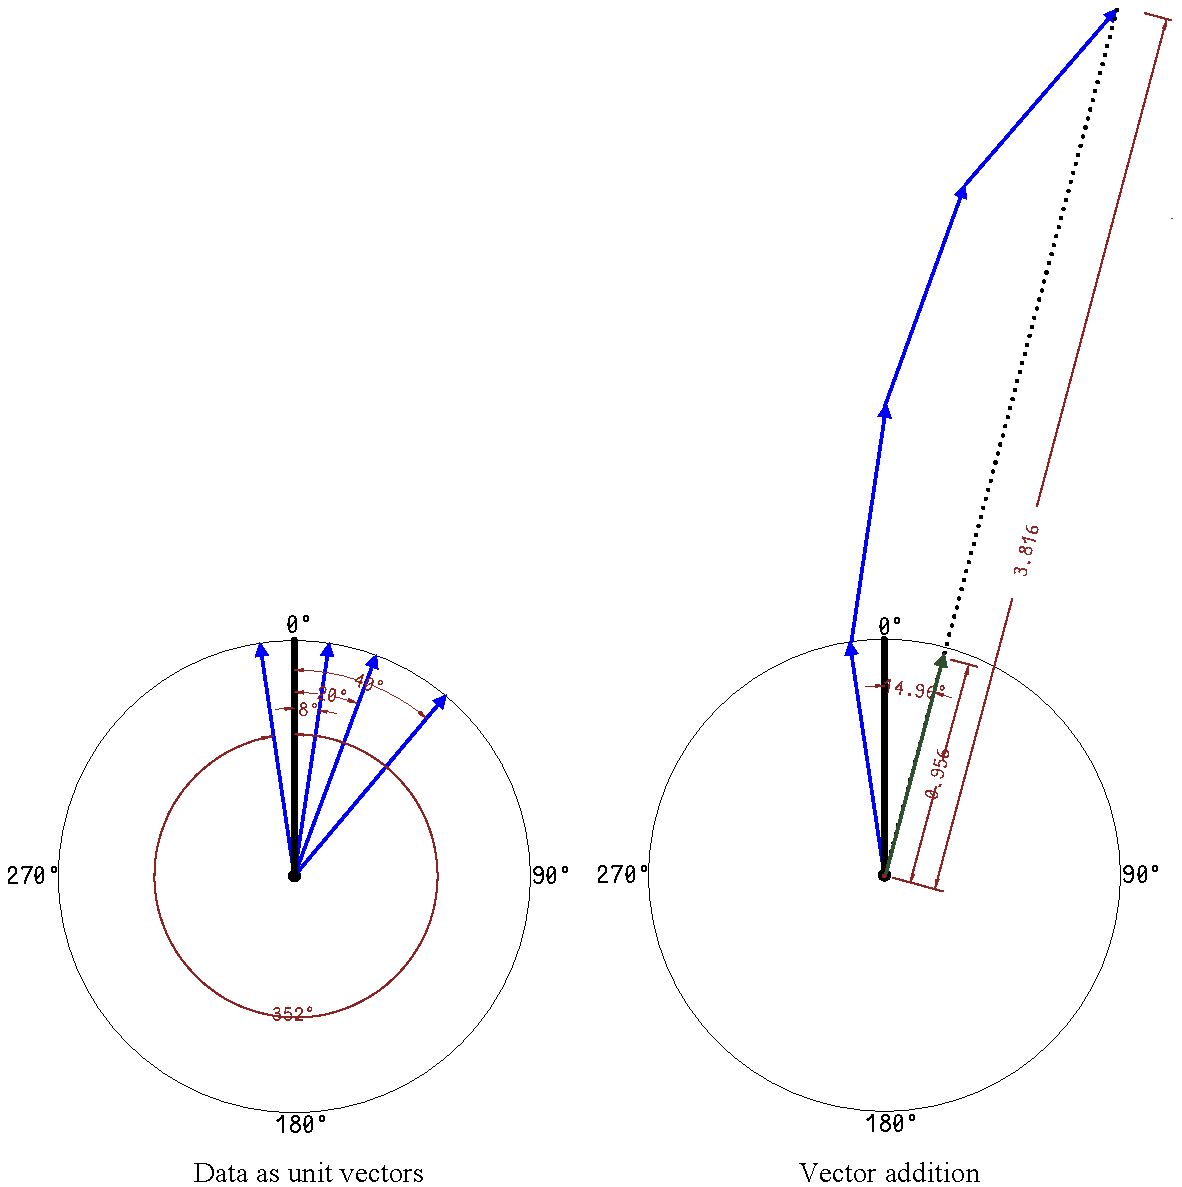
\includegraphics[width=0.7\textwidth]{Graphics/CircularMean}
\end{figure}


The data are plotted as unit vectors from the centre of a unit circle, with the angle identifying the direction of the vector (see fig. \ref{fig:CircMean}). The mean vector is then determined by vector addition of the data vectors.
\begin{eqnarray}
 \nonumber % Remove numbering (before each equation)
  C_p &=& \sum_{i = 1}^n{\cos(p \theta_i)} \\
 \nonumber
  S_p &=& \sum_{i = 1}^n{\sin(p \theta_i)} \\
 \nonumber
  R_p &=& \sqrt{C^2_p + S^2_p}, \quad [0\ldots n] \\
 \nonumber
 \bar{R}_p &=& R_p / n, \quad [0\ldots 1] \\
 \nonumber
  \bar{\theta}_p &=& \sin^{-1}(S_p/R_p) = \cos^{-1}(C_p/R_p) = \left\{
     \begin{array}{lr}
        \cos^{-1}(C_p/R_p) = \cos^{-1}(0) = \pi/2 &  C_p = 0          \\
        \tan^{-1}(S_p/C_p) + \pi                  &  C_p < 0          \\
        \tan^{-1}(S_p/C_p)                        &  S_p > 0, C_p > 0 \\
        \tan^{-1}(S_p/C_p) + 2\pi                 &  S_p < 0, C_p > 0
     \end{array}
   \right.
\end{eqnarray}
where \skalar{\bar{\theta}_p} is the mean vector direction and \skalar{\bar{R}_p} is the resultant length with respect to a positive whole number \skalar{p}. For the simple mean, \( p = 1 \), but higher values are required for some of the following. The sample statistics \skalar{\bar{\theta}_1} and \skalar{\bar{R}_1} (usually written \skalar{\bar{\theta}, \bar{R}}) estimate the population parameters \skalar{\mu} and \skalar{\rho}.

\begin{lstlisting}[caption=Arithmetic mean of circular data]
  FUNCTION MeanVector (TransformedData : VectorTyp; p : word) : ComplexTyp;

  VAR C, S, R, theta, Datum : float;
      n, i                  : WORD;

  BEGIN
     n  := VectorLength(TransformedData);
     C := 0;
     S := 0;
     FOR i := 1 TO n DO
       BEGIN
         Datum := GetVectorElement(TransformedData, i);
         C := C + Cos(p * Datum);
         S := S + Sin(p * Datum);
       END;
    R := Sqrt(C*C + S*S) / n;
    CASE signum(C) OF
      0 : theta := Const_pi / 2;    // arccos(C/R) = arccos(0)
     -1 : theta := ArcTan(S/C) + Const_pi;
      1 : CASE signum(S) OF
            1 :  theta := ArcTan(S/C);
           -1 :  theta := ArcTan(S/C) + Const_2pi;
            0 :  theta := 0;
      END;
    END;
    Result := ComplexInit(R, theta); // convert to complex number
  END;
\end{lstlisting}

\subsection{Spread}

The sample circular variance \skalar{V} and the sample circular standard deviation \skalar{v}  are calculated as follows:
\begin{eqnarray}
  V      &=& 1 - \bar{R}_1, \quad [0\ldots 1] \\
  v      &=& \sqrt{-2\ln(1-V)} = \sqrt{-2\ln(\bar{R}_1)}, \quad [0\ldots \infty]
\end{eqnarray}

\begin{lstlisting}[caption=Circular variance and standard deviation]
  FUNCTION CircularVariance (R : float) : float;

  BEGIN
    Result := 1 - R;
  END;

  FUNCTION CircularStandardDeviation (R : float) : float;

  BEGIN
    Result := sqrt(-2 * ln(R));
  END;
\end{lstlisting}

The maximum likelihood estimator for the parameter \skalar{\kappa} of the \Name{von Mieses} distribution is given by the approximation
\begin{equation}
  \hat{\kappa} = \left\{
          \begin{array}{l@{\;}l}
             2 \bar{R} + \bar{R}^3 + \frac{5 \bar{R}^5}{6}  & \quad \forall\ \bar{R} < 0.53 \\
             -0.4 + 1.39 \bar{R} + \frac{0.43}{1-\bar{R}}   & \quad \forall\ \bar{R} \in [0.53\ldots 0.85[\\
             \frac{1}{\bar{R}^3 - 4 \bar{R}^2 + 3 \bar{R}}  & \quad \forall\ \bar{R} \geq 0.85
          \end{array}
        \right.
\end{equation}
which for \( n \leq 15 \) needs a small sample correction
\begin{equation}
  \hat{\kappa}_c = \left\{
          \begin{array}{l@{\;}l}
             \max((\hat{\kappa} - 2/(n\hat{\kappa})), 0) & \quad \forall\ \hat{\kappa} < 2 \\
             (n-1)^3 \frac{\hat{\kappa}}{n^3 + n}        & \quad \forall\ \hat{\kappa} \geq 2
          \end{array}
        \right.
\end{equation}

\begin{lstlisting}[caption=Maximum likelihood estimator of \skalar{\kappa}]
  FUNCTION Kappa (R : float; n : WORD) : float;

  VAR k : float;

  BEGIN
    IF R < 0.53
      THEN
        k := 2*R + R*R*R + 5*pot(R, 5)/6
      ELSE
        IF R < 0.85
          THEN k := -0.4 + 1.39*R + 0.43/(1-R)
          ELSE k := 1 / (R*R*R - 4*R*R + 3*R);
    IF n <= 15  // small sample correction
      THEN
        IF k < 2
          THEN k := max((k - 2/(n*k)), 0)
          ELSE k := pot(Pred(n), 3) * k / (n*n*n + n);
    Result := k;
  END;
\end{lstlisting}

The median direction of a circular sample is the diameter of the circle that divides the data into two groups of equal size. However, we can use the median function for linear data only if all data are on the same side of the \texttt{0}-point.

\begin{lstlisting}[caption=Median of circular data]
  FUNCTION MedianDirection (TransformedData : VectorTyp) : float;

  BEGIN
    Result := Median(TransformedData);
  END;
\end{lstlisting}

\subsection{Higher moments}

The \skalar{p}th trigonometric moment (centred, that is, relative to the mean direction) is calculated by
\begin{equation}
  \mu_p = \frac{1}{n} \sum_{i=1}^n(\cos(p (\theta_i - \bar{\theta}))) + \imath \frac{1}{n} \sum_{i=1}^n(sin(p (\theta_i - \bar{\theta})))
\end{equation}

\begin{lstlisting}[caption=p-th trigonometric moment]
  FUNCTION TrigonometricMoment (Data : VectorTyp; MeanAngle : float; p : WORD) : ComplexTyp;

  VAR n, i : WORD;
      SumCos, SumSin, x : float;

  BEGIN
    n := VectorLength(Data);
    SumCos := 0;
    SumSin := 0;
    FOR i := 1 TO n DO
      BEGIN
        x := GetVectorElement(Data, i);
        SumSin := SumSin + Sin(p * (x - MeanAngle));
        SumCos := SumCos + Cos(p * (x - MeanAngle));
      END;
    Result := ComplexInit(SumCos/n, SumSin/n);
  END;
\end{lstlisting}

From these moments, we can calculate the \skalar{p}-th centred mean vector just like we did for the mean vector above:
\begin{lstlisting}[caption=p-th centered mean]
  function CenteredMean(Moment : ComplexTyp) : ComplexTyp;

  var S, C, R, theta : float;

  BEGIN
    C := Re(Moment);
    S := Im(Moment);
    R := sqrt(C*C + S*S);
    CASE signum(C) OF
      0 : theta := Const_pi / 2;    // arccos(C/R) = arccos(0)
     -1 : theta := ArcTan(S/C) + Const_pi;
      1 : CASE signum(S) OF
            1 :  theta := ArcTan(S/C);
           -1 :  theta := ArcTan(S/C) + Const_2pi;
            0 :  theta := 0;
      END;
    END;
    Result := ComplexInit(R, theta); // convert to complex number
  END;
\end{lstlisting}

From the first and second trigonometric moments \skalar{m_1, m_2} we calculate the circular dispersion as \( \delta = \frac{1 - \mu_2}{2 \mu_1^2} \)

\begin{lstlisting}[caption=Circular dispersion]
  FUNCTION CircularDispersion (TransformedData : VectorTyp; Mean : ComplexTyp) : float;

  var n, i         : word;
      R, theta, m2 : float;

  BEGIN
    n := VectorLength(TransformedData);
    theta := Im(Mean);
    m1 := Re(TrigonometricMoment(TransformedData, theta, 1));
    m2 := Re(TrigonometricMoment(TransformedData, theta, 2));
   Result := (1 - m2) / (2 * m1 * m1);
  END;
\end{lstlisting}

\subsubsection{Skew}

Skew can be calculated either from the original (\skalar{s}) or from the centred data (\skalar{s_0})
\begin{eqnarray}
  s   &=& \frac{1}{n} \sum_{i=1}^n sin(2 (\theta_i - \bar{\theta})) \\
  s_0 &=& \frac{R_2 \sin(\theta_2 - 2 \theta)}{1 - R}
\end{eqnarray}
A value close to \num{0} indicates a symmetrical distribution around the mean direction.

\begin{lstlisting}[caption=Circular skew]
  FUNCTION CircularSkew (TransformedData : VectorTyp; Mean : ComplexTyp) : float;

  VAR n, i          : WORD;
      theta, SumSin : float;

  BEGIN
    n := VectorLength(TransformedData);
    theta := Im(Mean); // mean angle
    SumSin := 0.0;
    FOR i := 1 TO n DO
      SumSin := SumSin + sin(2 * (GetVectorElement(TransformedData, i) - theta));
    Result := SumSin / n;
  END;


  FUNCTION CenteredCircularSkew (Mean1, Mean2 : ComplexTyp) : float;

  VAR theta1, theta2, R1, R2 : float;

  BEGIN
    theta1 := Im(Mean1);
    R1 := Re(Mean1);
    theta2 := Im(Mean2);
    R2 := Re(Mean2);
    Result := pot(1-R1, 2/3);
    IF Result = 0
      THEN
        BEGIN
          CircleError := true;
          WriteLn('Error: Circular skew when resultant length is 1');
          EXIT;
        END;
    Result := R2 * sin(theta2 - 2*theta1) / Result;
  END;
\end{lstlisting}

\subsubsection{Kurtosis}

The circular kurtosis we also can calculate centred or non-centred
\begin{eqnarray}
  k   &=& \frac{1}{n} \sum_{i=1}^n cos(2 (\theta_i - \bar{\theta})) \\
  k_0 &=& \frac{R_2 \cos(\theta_2 - 2 \bar{\theta}) - R^4}{(1 - R)^2}
\end{eqnarray}
, a value close to \num{1} indicates a strongly peaked distribution. If the data come from a \Name{von Mieses} distribution, then \( k_0 = 0 \).

\begin{lstlisting}[caption=Circular kurtosis]
  FUNCTION CircularKurtosis (TransformedData : VectorTyp; Mean : ComplexTyp) : float;

  VAR n, i          : WORD;
      theta, SumCos : float;

  BEGIN
    n := VectorLength(TransformedData);
    theta := Im(Mean); // mean angle
    SumCos := 0.0;
    FOR i := 1 TO n DO
      SumCos := SumCos + cos(2 * (GetVectorElement(TransformedData, i) - theta));
    Result := SumCos / n;
  END;


  FUNCTION CenteredCircularKurtosis (Mean1, Mean2 : ComplexTyp) : float;

  VAR theta1, theta2, R1, R2 : float;

  BEGIN
    theta1 := Im(Mean1);
    R1 := Re(Mean1);
    theta2 := Im(Mean2);
    R2 := Re(Mean2);
    Result := sqr(1-R1);
    IF Result = 0
      THEN
        BEGIN
          CircleError := true;
          WriteLn('Error: Circular kurtosis when resultant length is 1');
          EXIT;
        END;
    Result := (R2 * cos(theta2 - 2*theta1) - pot(R1, 4)) / Result;
  END;
\end{lstlisting}

\subsection{Confidence interval for mean direction}

If the allowable error is \skalar{\delta}, then the confidence interval \( d(1 - \delta) \) is computed by
\begin{equation}
  d = \left\{
          \begin{array}{l@{\;}l}
             \arccos\left[\frac{\sqrt{\frac{2 n (2 {(\bar{R} n)^2 - n \chi^2_{\delta,1}})}{4 n - \chi^2_{\delta,1}}}}{\bar{R} n} \right]    & \quad \forall\ \bar{R} \leq 0.9 \wedge \bar{R} > \sqrt{\frac{\chi^2_{\delta,1}}{2n}} \\
              & \\
             \arccos\left[\frac{\sqrt{n - {n^2 - (\bar{R} n)^2} \exp(\frac{\chi^2_{\delta,1}}{n})}}{\bar{R} * n} \right]    & \quad \forall\ \bar{R} > 0.9 \\
          \end{array}
        \right.
\end{equation}
The confidence interval is then \( \bar{\theta} \pm d \).

\begin{lstlisting}[caption=Confidence interval of circular mean]
  FUNCTION ConfidenceInterval (R, delta : float; n : WORD) : float;

  VAR Rn, chi : float;
      c       : CHAR;

  BEGIN
    Rn := R * n;
    chi := SignificanceLimit_Chi2(delta, 1);
    IF R > 0.9
      THEN
        Result := arccos(Sqrt(n - (n*n - Rn*Rn) * Exp(chi/n))/Rn)
      ELSE IF R > Sqrt(chi/(2*n))
             THEN
               Result := arccos(Sqrt((2 * n * (2*Rn*Rn - n*chi)) / (4*n - chi))/Rn)
             ELSE
               BEGIN
                 c := WriteErrorMessage('Confidence interval of mean angle: vector length to small');
                 CircleError := TRUE;
                 EXIT;
               END;
  END;
\end{lstlisting}

\section{Pseudo-random variables }

\begin{figure}
 \caption{\capstart Random variables of different distributions. \emph{Right}: Uniformly distributed. \emph{Left + middle}: \Name{von Mieses} distributed with different mean direction \skalar{\bar{\theta}} and spread \skalar{\kappa}.}
 \label{fig:CircRand}
 \centering
 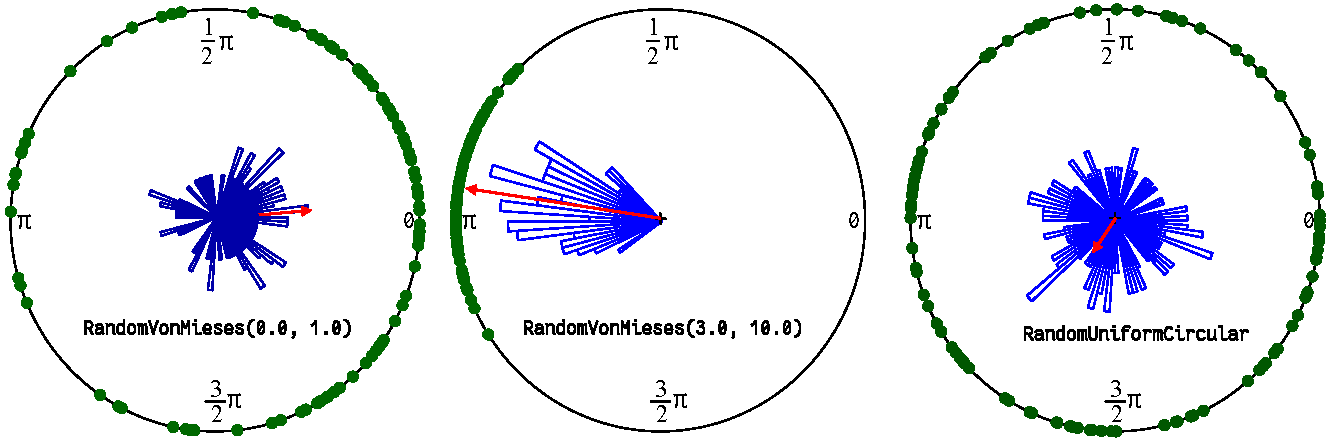
\includegraphics[width=\textwidth]{Graphics/c1-mean}
\end{figure}


The following routine returns a \Name{von Mieses}-distributed pseudo-random number, the algorithm is described in \parencite{Bar-95} (see fig. \ref{fig:CircRand}).

\begin{lstlisting}[caption=von Mieses distributed random number]
  FUNCTION RandomVonMieses(mu, kappa : float) : float;

  VAR s, u1, u2, theta : float;

  BEGIN
    IF kappa > 1.3
      THEN s := 1/Sqrt(kappa)
      ELSE s := Const_pi * Exp(-kappa);
    REPEAT
      u1 := Random;
      u2 := Random;
      theta := s*(2*u2 - 1) / u1;    // generate prospective value
      IF Abs(theta) < Const_pi       // rejection pre-TEST
        THEN
          IF ((kappa*theta*theta) < (4 - 4*u1))  // acceptance pre-TEST
            THEN
              BEGIN
                Result := ModuloTwoPi(theta + mu);
                EXIT;
              END
            ELSE
              IF ((kappa*Cos(theta)) > (2*Ln(u1) + kappa))
                THEN
                  BEGIN
                    Result := ModuloTwoPi(theta + mu);
                    EXIT;
                  END
               ELSE  // IF < THEN TRY again
        ELSE // IF > THEN TRY again
    UNTIL FALSE;
  END;
\end{lstlisting}

Random numbers uniformly distributed around the circle are a useful \texttt{0}-model:

\begin{lstlisting}[caption=Random data uniformly distributed over a circle]
  FUNCTION RandomUniformCircular : float;

  BEGIN
    Result := Random * Const_2pi;
  END;
\end{lstlisting}

\section{Statistical tests for a single circular data set}

\subsection{Do samples have a preferred direction}

These procedures test \textbf{\skalar{H_0}: The data are uniformly distributed} against \textbf{\skalar{H_1}: There is a preferred direction}.

\subsubsection{The \Name{Rayleigh}-test}

From the discussion above it is clear that the closer the data cluster toward a main direction, the larger the length of the mean vector becomes. Thus, \textbf{\skalar{H_0}} could also be phrased as \( \bar{R} = 0 \) and \textbf{\skalar{H_1}} as \( \bar{R} > 0 \). For \( n > 10 \) and \Name{von Mieses}-distributed data the probability for \textbf{\skalar{H_0}} becomes:
\begin{equation}
  P_0 \approx\ \exp \left[\sqrt{1 + 4n + 4(n^2 - R^2)} - (1 + 2n))\right]
\end{equation}
This test is suitable only for unimodal data. Note that in the formula \skalar{R} is used, not \( \bar{R} \). For consistency, the following function accepts \( \bar{R} \), however.

\begin{lstlisting}[caption=Rayleigh-test]
  FUNCTION Rayleigh (MeanVectorLength : float; n : WORD) : float;

  VAR c : CHAR;
      x : float;

  BEGIN
    IF (n < 10)
      THEN
        BEGIN
          c := WriteErrorMessage('Rayleigh test with less than 10 data points');
          CircleError := TRUE;
          EXIT;
        END;
    x := MeanVectorLength * n; // convert TO unscaled
    Result := Exp(Sqrt(1 + 4*n + 4*(n*n - x*x)) - (1 + 2*n));
  END;
\end{lstlisting}


\subsubsection{The \Foreign{omnibus} test of \Name{Hodges-Ajne}}

If the data are plotted on a circle, and a diameter is drawn through that circle, some data will be on one, the others on the other side of that diameter. The diameter line is then rotated until the number of data points on the ``wrong'' side (\skalar{m}) becomes minimal. Actually (at least in unimodal distributions), the diameter that produces minimal \skalar{m} must be the one at right angle to the mean vector. \skalar{m} will be the smaller the more directional the data are. This test is non-parametric and does not require the data to be \Name{von Mieses} distributed (hence ``\Foreign{omnibus}'' = Lat. ``for all'', here: irrespective of a data model). The probability, to observe a \skalar{m} this small for randomly distributed data becomes
\begin{equation}
  P_0 = \frac{1}{2^{n-1}}\ (n - 2m)\ \binom{n}{m}
\end{equation}
As a non-parametric test, this test is less powerful than the \Name{Rayleigh}-test.

\begin{lstlisting}[caption=Omnibus-test]
  FUNCTION HodgesAjne (TransformedData : VectorTyp; MeanAngle : float) : float;

  VAR StartAngle, StopAngle, x : float;
      i, m1, m2, n             : WORD;

  BEGIN
    StartAngle := ModuloTwoPi(MeanAngle - Nintey);
    StopAngle := ModuloTwoPi(MeanAngle + Nintey);
    IF StartAngle > StopAngle
      THEN
        BEGIN // exchange start- and stop angle
          x := StartAngle;
          StartAngle := StopAngle;
          StopAngle := x;
        END;
    n := VectorLength(TransformedData);
    m1 := 0;
    m2 := 0;
    FOR i := 1 TO n DO
      BEGIN
        x := GetVectorElement(TransformedData, i);
        IF (x >= StartAngle) AND (x <= StopAngle)
          THEN INC(m1)  // count # OF data points on either side of the diameter
          ELSE INC(m2);
      END;
    IF (m1 > m2) THEN m1 := m2; // peak on the other side of diameter
    Result := 1/pot(2, Pred(n)) * (n - 2*m1) * BinomialCoef(n, m1);
  END;
\end{lstlisting}


\subsubsection{The \skalar{\chi^2}-test}

Input parameters are the data vector (transformed to \( [0\ldots 2\pi] \)), the direction of the mean vector, and the number of sectors. Output data are the \skalar{\chi^2} and the degrees of freedom.

\begin{lstlisting}[caption=\skalar{\chi^2}-test for homogeneous distribution]
  PROCEDURE ChiSqrTest (Data : VectorTyp; Direction : float; Sectors : WORD;
                        VAR ChiSqr : float; VAR dgf : WORD);

  VAR i, j, Counter, n, max : WORD;
      Expected, Angle,
      StartAngle,
      Start, Finish, x      : float;
      Dummy                 : CHAR;
      ErrorStr, s           : STRING;

  BEGIN
    n := VectorLength(Data);
    IF n < 8
      THEN
        BEGIN
          CircleError := TRUE;
          Dummy := WriteErrorMessage('Not enough data for ChiSqr-test (> 8 required)');
          EXIT;
        END;
    max := n DIV 4;
    IF max > 250 THEN max := 250;
    Expected := n / Sectors;
    IF Expected < 4
      THEN
        BEGIN
          CircleError := TRUE;
          Str(n:4, ErrorStr);
          Str(max:4, s);
          ErrorStr := ErrorStr + 'Data points allow at most ' + s + ' sectors';
          Dummy := WriteErrorMessage(ErrorStr);
          EXIT;
        END;
    ChiSqr := 0.0;
    Angle := Const_2pi / Sectors;
    StartAngle := Direction - 0.5 * Angle;
    dgf := Pred(Sectors);
    FOR i := 1 TO Sectors DO
      BEGIN
        Start := StartAngle + Pred(i) * Angle;
        Finish := Start + Angle;
        Counter := 0;
        FOR j := 1 TO n DO
          BEGIN
            x := GetVectorElement(Data, j);
            IF (Start <= Const_2pi) AND (Finish <= Const_2pi)
              THEN
                IF (x > Start) AND (x < Finish)
                  THEN INC(Counter)
                  ELSE // outside SECTOR
              ELSE
                IF (Start < Const_2pi) AND (Finish > Const_2pi)
                  THEN
                    IF ((x > Start) AND (x < Const_2pi)) OR (x < ModuloTwoPi(Finish))
                      THEN INC(Counter)
                      ELSE
                  ELSE
                    IF (x > ModuloTwoPi(Start)) AND (x < ModuloTwoPi(Finish))
                      THEN INC(Counter);
            END; // FOR j
         ChiSqr := ChiSqr + Sqr(Counter - Expected) / Expected;
      END;  // FOR i
  END;
\end{lstlisting}

\subsubsection{\skalar{V}-test for uniformity against a suspected direction}

Sometimes one can specify an expected value for the mean vector direction \emph{before} an experiment is undertaken. Then a test for randomness needs not exclude all other possible models, hence the ``\skalar{V}-test'' is more efficient \parencite{Gre-55}. Thus, \textbf{\skalar{H_0}: The data are homogeneously distributed} against \textbf{\skalar{H_1}: The data cluster around a hypothetical direction \skalar{\theta_A}}. Note that the test applies only to randomness, it is not useful to decide whether the mean direction coincides with the expected direction. The test statistics is
\begin{equation}
  V = \sqrt{\frac{2}{n}}\ R\ cos(\bar{\theta} - \theta_A)
\end{equation}
However, if the test fails to reach significance, it is unclear whether the data are uniformly distributed or the expected value was wrong.

\begin{lstlisting}[caption=V-test for random distribution against suspected direction]
  FUNCTION HomewardComponent (n : WORD; Mean : ComplexTyp; Expected : float) : float;

  VAR Length, Phi, v : float;

  BEGIN
    Polar(Mean, Length, Phi);
    Phi := ModuloTwoPi(Phi);
    v := Length * Cos(Phi - Expected);
    Result := Sqrt(2*n) * v;
  END;
\end{lstlisting}

\subsubsection{\Name{Rao}'s spacing test}

If circular data are randomly distributed, then their distance from each other should be roughly \( \lambda = \frac{360}{n} \) \parencite{Rao-76}. If the data are clustered, some distances should be significantly larger than others. The test statistics becomes:
\begin{equation}
  U = \frac{1}{2} \sum_{i=1}^{n-1}{|(\theta_{i+1} - \theta_i) - \lambda|}
\end{equation}
\Name{Rao}'s test can be used for uni- and multimodal data, the critical values of \skalar{U} are tabulated in \parencite{Rus-95}.

\begin{lstlisting}[caption=\Name{Rao}'s test]
  FUNCTION Rao (TransformedData : VectorTyp) : float;

  VAR T, SumT, Expected : float;
      i, n              : WORD;

  BEGIN
    n := VectorLength(TransformedData);
    Expected := Const_2pi / n;
    SumT := 0;
    FOR i := 2 TO n DO
      BEGIN
        T := GetVectorElement(TransformedData, i) - GetVectorElement(TransformedData, Pred(i));
        SumT := SumT + Abs(T - Expected);
      END;
    T := Const_2pi + GetVectorElement(TransformedData, 1) - GetVectorElement(TransformedData, n);
    SumT := SumT + Abs(T - Expected);
    Rao := 0.5 * SumT;
  END;
\end{lstlisting}

\subsubsection{\Name{Kuipers}'s test against a suspected distribution}

\Name{Kuipers}'s test compares a given distribution of data with a theoretical model. The data matrix contains in the first column the angle, in the second the measured cumulative frequency and in the third the theoretical cumulative frequency (both in the range \( [0\ldots 1] \)). Returned are \skalar{V_n} and \skalar{K}.

\begin{lstlisting}[caption=\Name{Kuipers}'s test]
  PROCEDURE Kuipers (Data : MatrixTyp; VAR K, U : float);

  VAR DPlus, DMinus, c, vSqr, cvn, vSum,
      Diff, Diff1, Diff2, Vn, vMean, x    : float;
      n, i                                : WORD;
      xVector, yVector,
      bVector                             : VectorTyp;

  BEGIN
    n := MatrixRows(Data);
    GetColumn(Data, 1, xVector);
    GetColumn(Data, 2, yVector);
    GetColumn(Data, 3, bVector);
    vSum := NeumaierSum(bVector);
    vMean := vSum / n;
    DPlus := 0.0;
    DMinus := 0.0;
    vSqr := 0.0;
    cvn := 0.0;
    FOR i := 1 TO n DO
      BEGIN
        x := GetVectorElement(bVector, i);
        Diff  := GetVectorElement(yVector, i) - x;
        Diff1 := GetVectorElement(yVector, Pred(i)) - x;
        Diff2 := GetVectorElement(yVector, Succ(i)) - x;
        IF Diff  > DPlus THEN DPlus := Diff;
        IF Diff1 > DPlus THEN DPlus := Diff1;
        IF Diff  < DMinus THEN DMinus := Diff;
        IF Diff1 < DMinus THEN DMinus := Diff1;
        c := Pred(2 * i);
        cvn := cvn + c * GetVectorElement(bVector, i) / n;
        vSqr := vSqr + Sqr(GetVectorElement(bVector, i));
      END;  // FOR
    Vn := (DPlus + Abs(DMinus)) * Sqrt(n);
    K := Vn;
    U := vSqr - cvn + n * (1/3 - Sqr(vMean - 0.5));
    DestroyVector(xVector);
    DestroyVector(yVector);
    DestroyVector(bVector);
  END;
\end{lstlisting}

The following routine creates the table with cumulative frequencies needed by \Name{Kuipers}'s test.

\begin{lstlisting}[caption=Create frequency table]
  procedure CalculateCumulativeFrequencies (Data : VectorTyp; FullCircle : float;
                                        var Result : MatrixTyp);

  var i, n : word;
      Wert : float;
      D    : VectorTyp;

  begin
    n := VectorLength(Data);
    CopyVector(Data, D);
    ShellSort(D);
    for i := 1 to n do
     begin
       Wert := GetVectorElement(D, i);
       SetMatrixElement(Result, i, 1, Wert);
       SetMatrixElement(Result, i, 2, i/n);
       SetMatrixElement(Result, i, 3, Wert/FullCircle);
     end;
    DestroyVector(D);
  end;
\end{lstlisting}

\subsubsection{One sample \skalar{t}-test}

This test is used to test \textbf{\skalar{H_0}: The population mean angle \skalar{\bar{\theta}} is equal to \skalar{\theta_0}} against \textbf{\skalar{H_1}: The population mean angle \skalar{\bar{\theta}} is different from \skalar{\theta_0}}. This test is performed by checking if \( \theta_0 \in \bar{\theta} \pm d(1-\delta) \), that is, \skalar{\theta_0} is between the upper and lower confidence limits.

\begin{lstlisting}[caption=One-sample \skalar{t}-test]
  FUNCTION OneSample (MeanAngle, R, delta, TestAngle : float; n : WORD) : BOOLEAN;

  VAR x : float;

  BEGIN
    x := ConfidenceInterval(R, delta, n);
    Result := (TestAngle > (MeanAngle - delta)) AND (TestAngle < (MeanAngle + delta));
  END;
\end{lstlisting}

\subsubsection{Binomial test for median angle}

This is a non-parametric test with a similar purpose as the one-sample test, however, it is based on the median rather than mean angle. \textbf{\skalar{H_0}: The population median angle \skalar{\breve{\theta}} is equal to \skalar{\theta_0}}. If \textbf{\skalar{H_0}} holds, then \skalar{\theta_0} should divide the data set into two nearly identical halfs, the number of data on either side should fall under the binomial distribution \( k = B(n, 0.5) \).

\subsection{Symmetry around \skalar{\breve{\theta}}}

If the data set is symmetrical around \skalar{\breve{\theta}}, then the median circular distance of the data points from the median \skalar{\breve{\theta}} should be zero. This can be tested by a \Name{Wilcoxon} signed rank test.

\subsection{Grouped data}

The data matrix contains circular data in grouped form: first column the middle of the range of angles, the second column the counts. The angles must be distributed across the circle evenly.

\begin{lstlisting}[caption=Mean direction of grouped data]
  FUNCTION MeanVectorGrouped (Transformed : MatrixTyp; Difference : float) : ComplexTyp;

  VAR Total, n, i, j : WORD;
      x, y, z,
      Length, Angle  : float;
      Coord          : ComplexTyp;

  BEGIN
      n := MatrixRows(Transformed);
      Total := 0;
      x := 0.0;
      y := 0.0;
      FOR i := 1 TO n DO
        BEGIN
          j := Round(GetMatrixElement(Transformed, i, 2));
          z := GetMatrixElement(Transformed, i, 1);
          Total := Total + j;
          x := x + j * Cos(z);
          y := y + j * Sin(z);
        END;
      x := x / Total;
      y := y / Total;
      Coord := ComplexInit(x, y);      // Re, Im
      Polar(Coord, Length, Angle);     // polar coordinates
      z := Difference / 2;
      z := z / Sin(z);
      Length := Length * z;            // correct quantisation error
      Result := Rect(Length, Angle);   // back TO cartesian coordinates }
  END;
\end{lstlisting}

\section{Multi-sample tests}

\subsection{\Name{Watson-Williams}-test: two vectors with circular data}

This test is the circular equivalent of the two-sample \skalar{t}-test for linear data, it assesses the question whether \skalar{s} data sets come from distributions with the same mean angle \parencite{wat-56, Ste-69}.
\begin{equation}
  F = K \frac{(n - s)(\sum_{j=1}^s(R_j - R))}{(s-1) (n - \sum_{j=1}^s(R_j))}, \quad K = 1 + \frac{3}{8\kappa}
\end{equation}
where \skalar{R_j} is the separate mean vector length for the \skalar{j}th group. \skalar{\kappa} is an estimator for the dispersion of the \Name{von Mieses} distribution. The resulting test statistics is compared with the critical value of \skalar{F_{\delta, 1, n-2}}.

The test is relatively robust against violations of the \Name{von Mieses} distribution, as long as all groups have at least \num{5} members.

\begin{lstlisting}[caption=Watson-Williams test]
  PROCEDURE WatsonWilliams (TransformedData1, TransformedData2 : VectorTyp);

  VAR Transformed3                                   : VectorTyp;
      Mean1, Mean2, Mean3                            : ComplexTyp;
      Length1, Length2, Length3, Phi1, Phi2, Phi3,
      x, r, g, F, P0                                 : float;
      i, n1, n2, n3, nMean                           : WORD;
      hst                                            : STRING;

   BEGIN
    n1 := VectorLength(TransformedData1);
    n2 := VectorLength(TransformedData2);
    n3 := n1 + n2;
    CreateVector(Transformed3, n3, 0.0);
    FOR i := 1 TO n1 DO
      SetVectorElement(Transformed3, i, GetVectorElement(TransformedData1, i));
    FOR i := 1 TO n2 DO
      SetVectorElement(Transformed3, n1+i, GetVectorElement(TransformedData2, i));
    Mean1 := MeanVector(TransformedData1);
    Polar(Mean1, Length1, Phi1);
    Phi1 := ModuloTwoPi(Phi1);
    Mean2 := MeanVector(TransformedData2);
    Polar(Mean2, Length2, Phi2);
    Phi2 := ModuloTwoPi(Phi2);
    Mean3 := MeanVector(Transformed3);
    Polar(Mean3, Length3, Phi3);
    Phi3 := ModuloTwoPi(Phi3);
    r := (Length1 + Length2) / 2;
    nMean := (n1 + n2) DIV 2;
    g := 1 + 3 / (8 * Kappa(r, nMean));
    F := g * (Length1 + Length2 - Length3) / (n3 - (Length1 + Length2));
    P0 := Integral_F(F, 1, n3-2);
    Writeln('F = ', FloatStr(F, ValidFigures), ', f1 = 1, f2 = ', n3-2:4,
            ' => P0 = ' + FloatStr(P0, ValidFigures));
    DestroyVector(Transformed3);
  END;
\end{lstlisting}

\subsection{Circular \Name{Kruskal-Wallis}-test for equal median}

Non-parametric test for \textbf{\skalar{H_0}:  \( \breve{\theta}_1 = \breve{\theta}_2 = \ldots = \breve{\theta}_s \)} against \textbf{\skalar{H_1}: At least one of the data set has a different median}. The test works by first calculating the overall median of the combined data set. Then for each group \skalar{i} we calculate \skalar{m_i}, the number of samples \skalar{\theta_j^i} (\skalar{j}th sample in the \skalar{i}th group) where the distance \( d(\theta_j^i, \breve{\theta}) \) is negative. Then the test statistics
\begin{equation}
  x = \frac{N^2}{M (N-M)}\sum_{i=1}^s\frac{m_i^2}{n_i} - \frac{N M}{N - M}
\end{equation}
(\skalar{M, N} total over all groups, \skalar{m_i, n_i} within the \skalar{i}th group) is compared with the upper \skalar{1-\delta}th percentile of the \skalar{\chi^2(\delta, s-1)} distribution. The test is valid only if all \( n_i > 10 \).

\begin{lstlisting}[caption=Kruskal-Wallis test]
  FUNCTION KruskalWallis (TransformedData1, TransformedData2 : VectorTyp) : float;

  VAR Data3                            : VectorTyp;
      Median3, x, xmin, xmax, P           : float;
      i, n1, n2, n3, m1, m2, m                          : WORD;
      c                                              : CHAR;

  BEGIN
    n1 := VectorLength(TransformedData1);
    n2 := VectorLength(TransformedData2);
    n3 := n1 + n2;
    IF (n1 <= 10) OR (n2 <= 10)
      THEN
        BEGIN
          c := WriteErrorMessage('Circular Kruskal-Wallis test: n > 10 required for all groups');
          CircleError := TRUE;
          EXIT;
        END;
    CreateVector(Data3, n3, 0.0);
    FOR i := 1 TO n1 DO
      SetVectorElement(Data3, i, GetVectorElement(TransformedData1, i));
    FOR i := 1 TO n2 DO
      SetVectorElement(Data3, n1+i, GetVectorElement(TransformedData2, i));
    ShellSort(Data3);
    Median3 := MedianDirection(Data3);
    xmin := ModuloTwoPi(Median3 + Nintey);
    xmax := ModuloTwoPi(Median3 - Nintey);
    m1 := 0;
    FOR i := 1 TO n1 DO
      BEGIN
        x := GetVectorElement(TransformedData1, i);
        IF (x > xmin) AND (x < xmax) THEN INC(m1);
      END;
    m2 := 0;
    FOR i := 1 TO n2 DO
      BEGIN
        x := GetVectorElement(TransformedData2, i);
        IF (x > xmin) AND (x < xmax) THEN INC(m2);
      END;
    m := m1 + m2;
    P := n3*n3 / (m * (n3 - m)) * (m1*m1/n1 + m2*m2/n2) - n3 * m / (n3 - m);
    Result := IntegralChi(P, 1);
    Writeln('Chi^2 = ', FloatStr(P, ValidFigures), ' with 1 degrees of freedom, P0 = ',
            FloatStr(x, ValidFigures));
    DestroyVector(Data3);
  END;
\end{lstlisting}

\subsection{Difference between two vectors}

Calculates the cumulative frequencies of both data vectors and calculates \Name{Kuiper}'s \skalar{V} und \Name{Whatson}'s \skalar{U^2}. The data vectors must be sorted.

\begin{lstlisting}[caption=Difference between two vectors]
  PROCEDURE Difference (Data1, Data2 : VectorTyp; VAR KuipersV, WatsonsUSqr : float);

  TYPE ListenRecTyp = RECORD
                        Angle, k1, k2 : float;
                      END;

  VAR n1, n2, Cumulative1, Cumulative2                  : WORD;
      Diff, Dif, DifSqr, DifPos, DifNeg, Angle1, Angle2 : float;
      ListenRec                                         : ListenRecTyp;
      Liste                                             : FiFo;

  BEGIN
    n1 := VectorLength(Data1);
    n2 := VectorLength(Data2);
    ShellSort(Data1);
    ShellSort(Data2);
    Cumulative1 := 0;
    Cumulative2 := 0;
    InitFiFo(Liste);
    WHILE (Cumulative1 < n1) AND (Cumulative2 < n2) DO          { Data durchlaufen, }
      BEGIN                                                     { cumulative Frequenzen }
        Angle1 := GetVectorElement(Data1, Succ(Cumulative1));   { erzeugen und in FIFO  }
        Angle2 := GetVectorElement(Data2, Succ(Cumulative2));   { Liste speichern }
        IF Angle1 < Angle2
          THEN
           BEGIN
               INC(Cumulative1);
               ListenRec.Angle := Angle1;
           END
          ELSE
           BEGIN
               INC(Cumulative2);
               ListenRec.Angle := Angle2;
           END;
        ListenRec.k1 := 1.0 * Cumulative1 / n1;
        ListenRec.k2 := 1.0 * Cumulative2 / n2;
        Put(Liste, ListenRec, SizeOf(ListenRec));
      END; { while }
    WHILE (Cumulative1 < n1) DO                               { eventuell übrig gebliebene }
     BEGIN                                                    { Elemente aus 1. Datasatz  }
       INC(Cumulative1);                                      { bearbeiten }
       ListenRec.k1 := 1.0 * Cumulative1 / n1;
       ListenRec.k2 := 1.0 * Cumulative2 / n2;
       ListenRec.Angle := GetVectorElement(Data1, Cumulative1);
       Put(Liste, ListenRec, SizeOf(ListenRec));
     END;
    WHILE (Cumulative2 < n2) DO                               { dito für 2. Datasatz }
     BEGIN
       INC(Cumulative2);
       ListenRec.k1 := 1.0 * Cumulative1 / n1;
       ListenRec.k2 := 1.0 * Cumulative2 / n2;
       ListenRec.Angle := GetVectorElement(Data2, Cumulative2);
       Put(Liste, ListenRec, SizeOf(ListenRec));
     END;
    DifPos := 0.0;
    DifNeg := 0.0;
    Dif    := 0.0;
    DifSqr := 0.0;
    WHILE NOT EmptyFiFo(Liste) DO                             { Liste durchlaufen und }
      BEGIN                                                   { größte positive und   }
        Get(Liste, ListenRec, SizeOf(ListenRec));             { negative Difference suchen }
        Diff := ListenRec.k1 - ListenRec.K2;
        IF Diff > DifPos THEN DifPos := Diff;
        IF Diff < DifNeg THEN DifNeg := Diff;
        Dif := Dif + Diff;                                    { aufsummieren für Watson's Test }
        DifSqr := DifSqr + Sqr(Diff);
      END;
    KuipersV := n1 * n2 * (DifPos - DifNeg);
    WatsonsUSqr := n1 * n2 / Sqr(n1+n2) * (DifSqr - Sqr(Dif) / (n1+n2));
  END;
\end{lstlisting}

Under the condition that the data are \Name{von-Mises}-distributed, the following routine calculates the \skalar{F}-value for \textbf{\skalar{H_0}: \( \kappa_1 = \kappa_2 \)} against \textbf{\skalar{H_1}: \( \kappa_1 \neq \kappa_2 \)}. The probability of \skalar{H_0} is then obtained by integrating the \skalar{F}-distribution with \skalar{n_1, n_2} degrees of freedom. If \( F < 1 \), the integration has to be performed with \skalar{1/F} and exchanged degrees of freedom.

\begin{lstlisting}[caption=F-test]
  FUNCTION FTest (Data1, Data2 : VectorTyp) : float;

  VAR Mean1, Mean2                               : ComplexTyp;
      Angle1, Angle2, Length1, Length2, rMean    : float;
      n1, n2                                     : WORD;

  BEGIN
    n1 := VectorLength(Data1);
    Mean1 := MeanVector(Data1, 1);
    Polar(Mean1, Length1, Angle1);
    n2 := VectorLength(Data2);
    Mean2 := MeanVector(Data2, 1);
    Polar(Mean2, Length2, Angle2);
    Length1 := Length1 * n1;
    Length2 := Length2 * n2;
    rMean := (Length1 + Length2) / (n1 + n2);
    IF rMean < 0.7
      THEN
       BEGIN
         CH := WriteErrorMessage('Mean vectors to short, F-Test not applicable');
         CircleError := TRUE;
         EXIT;
       END;
    Result := Pred(n2) * (n1 - Length1) / (Pred(n1) * (n2 - Length2));
  END;
\end{lstlisting}

\Name{Wilcoxon}'s non-parametric test for \textbf{\skalar{H_0}: The data sets have the same standard deviation} vs. \textbf{\skalar{H_1}: The data sets have different standard deviations}. \texttt{Direction1} and \texttt{-2} contain either the mean direction of the data vectors, or a common homeward component. In the latter case, the test is for equal/unequal home-finding ability. The function returns the \Name{Wilcoxon-Mann-Whitney} \skalar{U}-value. All data must be in \( [0..2\pi] \).

\begin{lstlisting}[caption=Wilcoxon's non-parametric test for equal standard deviation]
  FUNCTION Wilcoxon (Data1, Data2 : VectorTyp; Direction1, Direction2 : float) : float;

  VAR U1, U2, x                       : float;
      n1, n2, Rank, i, j, Sum1, Sum2  : WORD;
      Diff1, Diff2                    : VectorTyp;

  BEGIN
    n1 := VectorLength(Data1);
    CreateVector(Diff1, n1, 0.0);
    FOR i := 1 TO n1 DO
     BEGIN
       x := Abs(GetVectorElement(Data1, i) - Direction1);
       IF x > Pi
         THEN SetVectorElement(Diff1, i, Const_2pi-x)
         ELSE SetVectorElement(Diff1, i, x);
     END;
    ShellSort(Diff1);
    n2 := VectorLength(Data2);
    CreateVector(Diff2, n2, 0.0);
    FOR i := 1 TO n2 DO
     BEGIN
       x := Abs(GetVectorElement(Data2, i) - Direction2);
       IF x > Pi
         THEN SetVectorElement(Diff2, i, Const_2pi-x)
         ELSE SetVectorElement(Diff2, i, x);
     END;
    ShellSort(Diff2);
    Rank := 1;
    j := 1;
    Sum1 := 0;
    Sum2 := 0;
    IF n1 < n2
      THEN
       BEGIN
         FOR i := 1 TO n1 DO
           BEGIN
             WHILE (GetVectorElement(Diff2, j) < GetVectorElement(Diff1, i)) DO
               BEGIN
                 INC(Sum2, Rank);
                 INC(Rank);
                 INC(j);
               END;
             INC(Sum1, Rank);
             INC(Rank);
           END;
         FOR i := j TO n2 DO
          BEGIN
            INC(Sum2, Rank);
            INC(Rank);
          END;
       END
      ELSE
       BEGIN
         FOR i := 1 TO n2 DO
           BEGIN
             WHILE (GetVectorElement(Diff1, j) < GetVectorElement(Diff2, i)) DO
               BEGIN
                 INC(Sum1, Rank);
                 INC(Rank);
                 INC(j);
               END;
             INC(Sum2, Rank);
             INC(Rank);
           END;
         FOR i := j TO n1 DO
          BEGIN
            INC(Sum1, Rank);
            INC(Rank);
          END;
       END;
    DestroyVector(Diff1);
    DestroyVector(Diff2);
    U1 := Sum1 - n1 * Succ(n1) / 2;
    U2 := Sum2 - n2 * Succ(n2) / 2;
    IF U1 < U2
      THEN Result := U1
      ELSE Result := U2;
  END;
\end{lstlisting}

\begin{lstlisting}[caption=]
  PROCEDURE DescribeBivariat (Data : MatrixTyp);

  VAR i, n1                                                     : WORD;
      SumX, SumY, a, b, c, d, r, SumXSqr, SumYSqr, SumXDevYDev,
      xSta, ySta, xMean, yMean, CoVariance, Correlation, Phi,
      Major, Minor, xMin, xMax, yMin, yMax                      : float;

  BEGIN
    SumX := 0.0;
    SumY := 0.0;
    SumXSqr := 0.0;
    SumYSqr := 0.0;
    SumXDevYDev := 0.0;
    n1 := MatrixRows(Data);
    xMin := MaxRealNumber;
    xMax := MinRealNumber;
    yMin := MaxRealNumber;
    yMax := MinRealNumber;
    FOR i := 1 TO n1 DO
      BEGIN
        a := GetMatrixElement(Data, i, 1);
        IF a > xMax THEN xMax := a;
        IF a < xMin THEN xMin := a;
        SumX := SumX + a;
        SumXSqr := SumXSqr + Sqr(a);
        a := GetMatrixElement(Data, i, 2);
        IF a > yMax THEN yMax := a;
        IF a < yMin THEN yMin := a;
        SumY := SumY + a;
        SumYSqr := SumYSqr + Sqr(a);
      END;
    xMean := SumX / n1;
    yMean := SumY / n1;
    xSta := Sqrt((SumXSqr - Sqr(SumX) / n1) / Pred(n1));
    ySta := Sqrt((SumYSqr - Sqr(SumY) / n1) / Pred(n1));
    Write('Mean x = ', FloatStr(xMean, ValidFigures), ' ± ', FloatStr(xSta, ValidFigures));
    Writeln('Mean y = ', FloatStr(yMean, ValidFigures), ' ± ', FloatStr(ySta, ValidFigures));
    FOR i := 1 TO n1 DO
      BEGIN
        a := GetMatrixElement(Data, i, 1) - xMean;
        b := GetMatrixElement(Data, i, 2) - yMean;
        SumXDevYDev := SumXDevYDev + a * b;
      END;
    CoVariance := SumXDevYDev / Pred(n1);
    Correlation := CoVariance / (xSta * ySta);
    A := Sqr(ySta);
    B := - CoVariance;
    C := Sqr(xSta);
    D := (1 - Sqr(Correlation)) * Sqr(xSta) * Sqr(ySta);
    R := Sqrt(Sqr(A - C) + 4 * Sqr(B));
    Phi := ArcTan(2 * B / (A - C - R));
    Major := Sqrt(2 * D / (A + C - R));
    Minor := Sqrt(2 * D / (A + C + R));
    Writeln('r = ', FloatStr(Correlation, ValidFigures), ' Φ = ', FloatStr(Phi, ValidFigures));
    Writeln('Major = ', FloatStr(Major, ValidFigures), ' Minor = ', FloatStr(Minor, ValidFigures));
    Write('Press any key: ');
  END;
\end{lstlisting}

\section{Regression and correlation}

\subsection{Linear dependent, circular independent variable}

In this case, the data are fitted to
\begin{equation}
  \hat{y} = a + b \cos(\theta - \theta_0) = a + b \cos(\theta) + c \sin(\theta)
\end{equation}
\skalar{\theta_0} is the peak phase (acrophase) of the data. In effect, the dependent variable is plotted onto a cylinder, rather than on a sheet of paper. This is called an \textbf{C-linear association} and is a special case of the \textbf{C-association}, which means any function that
\begin{itemize}
  \item{has exactly one maximum and one minimum over the range of \( [0\ldots 2\pi] \)}
  \item{has matching \(\hat{y}\) at \num{0} and \skalar{2\pi} (\Foreign{i.e.}, is periodic)}
\end{itemize}

\subsubsection{Degree of C-association}

The U-test gives the probability of \textbf{H\textsubscript{0}: The variables \skalar{\theta} and \AbsVec{x} are independent} (\(D_n = 0\)) against \textbf{H\textsubscript{1}: The variables \skalar{\theta} and \AbsVec{x} are C-associated} (\(D_n > 0\)):
\begin{eqnarray}
  D_n &=& a_n (T^2_c + T^2_s) \\
  T_c &=& \sum_{i=1}^n \AbsVec{x}_i \cos(\theta_i),\quad T_s = \sum_{i=1}^n\AbsVec{x}_i \sin(\theta_i) \\
  a_n &=& \left\{
              \begin{array}{lr}
              [1 + 5 \cot^2(\pi/n) + 4 \cot^4(\pi/n)]^{-1} & n\ \mathrm{even} \\
              2 \sin^4(\pi/n) / [1 + \cos(\pi / n)]^3      & n\ \mathrm{odd}
              \end{array}
          \right. \\
  U_n &=& 24 \frac{T^2_c + T_s^2}{n^3+n^2} \approx \chi^2_{2,\alpha} \\
  P(H_0) &=& \exp\left(-\frac{U_n^2}{2}\right)\quad \forall\ n > 100
\end{eqnarray}
\skalar{D_n} is a quantity in [0\ldots 1], with values near \num{0} suggesting that there is no C-association. It can be considered a correlation coefficient, for which \skalar{U_n} is the test statistics. For \( n \leq 100\), critical values are given in \parencite{Mar-76}. After correction of two obvious typos these follow an exponential equation
\begin{equation}
  y = a * (1 - b^n)
\end{equation}
with the parameters
\begin{tabular}{l|ccccc}
  \toprule
  \skalar{\alpha} & \skalar{a} & \skalar{\pm} & \skalar{b} & \skalar{\pm} &  \skalar{r^2}  \\
  \midrule
  0.10 & 4.608 & 0.008 & 0.668 & 0.004 & 0.986 \\
  0.05 & 5.909 & 0.026 & 0.773 & 0.004 & 0.987 \\
  0.01 & 8.912 & 0.064 & 0.865 & 0.003 & 0.991 \\
  \bottomrule
\end{tabular}

\begin{lstlisting}[caption=C-association between linear and circular data]
  FUNCTION CAssociation (CONST theta, Y : VectorTyp; VAR Sig : SignificanceType) : float;

  VAR Tc, Ts, an, Un, P, xi, ti : float;
      i, n                      : WORD;
      c                         : char;

    FUNCTION InterpolateCritical (Un : float; n : WORD) : float;
    // interpolates critical values in table A10 from Fisher (1993)

    const a10 = 4.608; a05 = 5.909; a01 = 8.912;
          b10 = 0.668; b05 = 0.773; b01 = 0.865;

    BEGIN
      if Un < (a10 * (1 - pot(b10, n)))                // critical value for 10%
        THEN Result := 1.0                             // to give it some value
        ELSE if Un < (a05 * (1 - pot(b05, n)))         // critical value for 5%
               THEN Result := 0.1
               ELSE if Un < (a01 * (1 - pot(b01, n)))  // critical value for 1%
                      THEN Result := 0.05
                      ELSE Result := 0.01;
    END;

  BEGIN
    n := VectorLength(theta);
    IF VectorLength(Y) <> n
      THEN
       BEGIN
         c := WriteErrorMessage('Linear-circular association: length of theta and x not equal');
         CircleError := true;
         EXIT;
       END;
    Tc := 0;
    Ts := 0;
    FOR i := 1 TO n DO
      BEGIN
        xi := GetVectorElement(Y, i);
        ti := GetVectorElement(theta, i);
        IF IsNaN(xi) OR IsNaN(ti)
          THEN // ignore data pair if either is NaN
          ELSE
            BEGIN
              Tc := Tc + xi*cos(ti);
              Ts := Ts + xi*sin(ti);
            END;
      END;
    IF ODD(n)
      THEN an := 2*pot(sin(Const_pi/n), 4) / pot(1+cos(Const_pi/n), 3)
      ELSE an := 1 / (1 + 5*pot(cot(Const_pi/n), 2) + 4*pot(cot(Const_pi/n), 4));
    Result := an * (Tc*Tc * Ts*Ts); // correlation coefficient
    WITH Sig DO
      BEGIN
        TestValue := 24 * (Tc*Tc * Ts*Ts) / (pot(n, 3) + pot(n, 2)); // test statistics Un
        Freedom := n;
        IF n > 100
          THEN P0 := exp(-pot(Un, 2)/2)
          ELSE P0 := InterpolateCritical(Un, n);
      END;
  END;
\end{lstlisting}

\subsubsection{Fitting a trigonometric polynomial}

The following procedure fits a dependent linear (\texttt{yData}) to an independent circular variable (\texttt{TransformedData}) using
\begin{equation}
  \hat{y} = m + a \cos(\theta - \theta_0)
\end{equation}
where \skalar{m} is the mean, \skalar{a} the amplitude and \skalar{\theta_0} the acrophase angle.

\begin{lstlisting}[caption=Fit a trigonometric polynomial]
  PROCEDURE TrigonometricPolynomial (const TransformedData, yData: VectorTyp;
                                     Periode : float);

  VAR i, n                                                     : WORD;
      Omega, t, s, c, y, tMax, tMin, yMax, yMin,
      SumY, SumC, SumS, SumCSqr, SumSSqr, SumYC,
      SumYS, SumCS, M, X, Z, Hilfs1, Hilfs2, Hilfs3, Hilfs4,
      Correlation, U, A, Phi, r, TEST, P0                       : float;
      Sig                                                      : SignificanceType;
      hstr                                                     : STRING;

  BEGIN
    n := VectorLength(TransformedData);
    IF n <> VectorLength(yData)
      THEN
        BEGIN
          ch := WriteErrorMessage('Linear-periodic correlation: Vectors of different lengths');
          CircleError := TRUE;
          EXIT;
        END;
    SumY := 0.0;
    SumC := 0.0;
    SumS := 0.0;
    SumCSqr := 0.0;
    SumSSqr:= 0.0;
    SumYC := 0.0;
    SumYS := 0.0;
    SumCS := 0.0;
    tMax := MinRealNumber;
    tMin := MaxRealNumber;
    yMax := MinRealNumber;
    yMin := MaxRealNumber;
    FOR i := 1 TO n DO
      BEGIN
        t := GetVectorElement(TransformedData, i);  // circular datum
        IF t > tMax THEN tMax := t;
        IF t < tMin THEN tMin := t;
        c := Cos(Periode*t);
        s := Sin(Periode*t);
        SumC := SumC + c;
        SumS := SumS + s;
        y := GetVectorElement(yData, i);            // linear datum
        IF y > yMax THEN yMax := y;
        IF y < yMin THEN yMin := y;
        SumY := SumY + y;
        SumCSqr := SumCSqr + Sqr(c);
        SumSSqr:= SumSSqr + Sqr(s);
        SumYC := SumYC + y * c;
        SumYS := SumYS + y * s;
        SumCS := SumCS + c * s;
      END;
    Hilfs1 := Sqr(SumC) + n * SumSSqr;
    Hilfs2 := (SumS * SumC * SumCS - Sqr(SumS) - n * Sqr(SumCS))
              / Hilfs1 - Sqr(SumS) / n + SumSSqr;
    Hilfs3 := (Sqr(SumS) * SumYC - n * SumYC * SumCS +
              SumCS * SumC * SumY - SumCS * SumC * SumS) / Hilfs1;
    Hilfs4 := (Sqr(SumS) * Sqr(SumC) - SumS * Sqr(SumC) * SumY)
              / (n * Hilfs1);
    Z := (SumYS + Hilfs3 + Hilfs4 - SumS * SumY / n) / Hilfs2;
    X := (n * SumYC - SumC * SumY + SumC * SumS - n * SumCS * Z)
         / Hilfs1;
    M := (SumY - SumC * X - SumS * Z) / n;
    A := Sqrt(Sqr(X) + Sqr(Z));
    CASE signum(X) OF
     1 : Phi := ArcTan(Z/X);
    -1 : IF x < 0 THEN Phi := Const_pi + ArcTan(Z/X);
     0 : CASE signum(y) OF
          1 : Phi := Nintey;                       {  90° }
         -1 : IF Y < 0 THEN Phi := Const_pi*3/2;   { 270° }
          0 :  BEGIN
                 CH := WriteErrorMessage('unknown akrophase angle ');
                 CircleError := TRUE;
                 EXIT;
               END;
         END;
    END;
    IF tMin > 0 THEN tmin := 0;
    IF yMin > 0 THEN yMin := 0;
    IF A < 0
      THEN hstr := '-'
      ELSE hstr := '+';
    Writeln('y = ', FloatStr(M, ValidFigures), ' ', HStr, ' ', FloatStr(A, ValidFigures),
            ' * cos(', FloatStr(Periode, ValidFigures), ' * t - ', FloatStr(Phi, ValidFigures), ')');
    CircularLinearCorrelation(TransformedData, yData, r, Sig);
    WITH Sig DO
      Writeln('Parametric: r = ', FloatStr(r, ValidFigures), ' chi2 = ',
       FloatStr(TestValue, ValidFigures), ' with 2 dgf, P(H0: r = 0) = ', FloatStr(P0, ValidFigures));
    LinearPeriodicRankCorrelation(TransformedData, yData, Correlation, u);
    Writeln('Non-Parametric r = ', FloatStr(Correlation, ValidFigures), ' U = ', FloatStr(U, ValidFigures));
  END;
\end{lstlisting}

\subsubsection{Correlation \skalar{r_{cl}} between linear and circular data}

We calculate the correlation between a directional random variable \skalar{\theta} and a linear random variable \AbsVec{x} by first calculating \( r_{sx} = r_p(\sin(\theta), \AbsVec{x}) \), \( r_{cx} = r_p(\cos(\theta), \AbsVec{x}) \) \( r_{sc} = r_p(\sin(\theta), \cos(\theta)) \), where \skalar{r_p} is \Name{Pearson}'s product-moment correlation (see section \ref{text:Pearson}). Then
\begin{equation}
  r_{cl} = \sqrt{\frac{r^2_{cx} + r^2_{sx} -  2 r^2_{cx} r^2_{sx} r^2_{cs}}{1 - r^2_{cs}}}
\end{equation}
and the test statistics \( \chi^2(n\ r_{cl}, 2) \).

\begin{lstlisting}[caption=Correlation between linear and circular data]
  PROCEDURE CircularLinearCorrelation (const TransformedData, yData: VectorTyp;
                                       VAR Correlation : float; VAR Sig : SignificanceType);

  VAR SinPhi, CosPhi, y : VectorTyp;
      n, i              : WORD;
      x, ryc, rys, rcs  : float;
      Hilfs             : char;

  BEGIN
    n := VectorLength(TransformedData);
    IF n <> VectorLength(yData)
      THEN
        BEGIN
          Hilfs := WriteErrorMessage('Linear-periodic correlation: Vectors of different lengths');
          CircleError := TRUE;
          EXIT;
        END;
    CreateVector(SinPhi, n, 0.0);
    CreateVector(CosPhi, n, 0.0);
    CreateVector(y, n, 0.0);
    FOR i := 1 TO n DO
      BEGIN
        x := GetVectorElement(TransformedData, i);
        SetVectorElement(SinPhi, i, Sin(x));
        SetVectorElement(CosPhi, i, Cos(x));
      END;
    ryc := PearsonProductMomentCorrelation(yData, CosPhi, sig);
    rys := PearsonProductMomentCorrelation(yData, SinPhi, sig);
    rcs := PearsonProductMomentCorrelation(CosPhi, SinPhi, sig);
    DestroyVector(SinPhi);
    DestroyVector(CosPhi);
    Correlation := (Sqr(ryc) + Sqr(rys) - 2 * ryc * rys * rcs) / (1 - Sqr(rcs)); // r^2
    WITH Sig DO
      BEGIN
        TestValue := n * Correlation;
        Freedom := 2;
        P0 := IntegralChi(TestValue, 2);
      END;
    Correlation := Sqrt(Correlation);
  END;
\end{lstlisting}

\subsubsection{Rank correlation}

Rank correlation between a linear and a periodic variable. For \Name{Spearman}'s rank correlation \skalar{r_s} between linear variables see chapter \ref{text:correlation}. Returns both \skalar{r} and the test statistics \skalar{U}. The test works even if the conditions for a parametric test are not met.

\begin{lstlisting}[caption=Rank correlation between linear and circular data]
  PROCEDURE RankXY (const TransformedData, yData : VectorTyp; var Ranks : VectorTyp);

  VAR n, i, Rank, MaxPos : WORD;
      Kopie              : MatrixTyp;
      Maximum, x         : float;

  BEGIN
    n := VectorLength(TransformedData);
    CreateMatrix(Kopie, n, 2, 0.0);
    SetColumn(Kopie, TransformedData, 1);
    SetColumn(Kopie, yData, 2);
    Rank := n;                       { Feld nach aufsteigenden x sortieren }
    REPEAT
      Maximum := MinRealNumber;
      FOR i := 1 TO Rank DO
        BEGIN
          x := GetMatrixElement(Kopie, i, 1);
          IF x > Maximum
            THEN
              BEGIN
                Maximum := x;
                MaxPos := i;
              END;
        END;
      x := GetMatrixElement(Kopie, MaxPos, 2);
      SetMatrixElement(Kopie, MaxPos, 1, GetMatrixElement(Kopie, Rank, 1));
      SetMatrixElement(Kopie, MaxPos, 2, GetMatrixElement(Kopie, Rank, 2));
      SetMatrixElement(Kopie, Rank, 1, Rank);
      SetMatrixElement(Kopie, Rank, 2, x);
      DEC(Rank);
    UNTIL (Rank = 0);
    Rank := n;                       { jetzt die Ränge der y-Elemente bestimmen }
    REPEAT
      Maximum := MinRealNumber;
      FOR i := 1 TO Rank DO
        BEGIN
          x := GetMatrixElement(Kopie, i, 2);
          IF x > Maximum
            THEN
              BEGIN
                Maximum := x;
                MaxPos := i;
              END;
        END;
      x := GetMatrixElement(Kopie, MaxPos, 1);
      SetMatrixElement(Kopie, MaxPos, 1, GetMatrixElement(Kopie, Rank, 1));
      SetMatrixElement(Kopie, MaxPos, 2, GetMatrixElement(Kopie, Rank, 2));
      SetMatrixElement(Kopie, Rank, 2, Maximum);
      SetMatrixElement(Kopie, Rank, 1, x);
      SetVectorElement(Ranks, Round(x), Rank);
      DEC(Rank);
    UNTIL (Rank = 0);
    DestroyMatrix(Kopie);
  END;


  PROCEDURE LinearPeriodicRankCorrelation (const TransformedData, yData: VectorTyp;
                                           VAR Correlation, U : float);

  VAR Ranks               : VectorTyp;
      n, i                : WORD;
      epsilon, x, y, c, s : float;
      hilfs               : char;

  BEGIN
    n := VectorLength(TransformedData);
    IF n <> VectorLength(yData)
      THEN
        BEGIN
          Hilfs := WriteErrorMessage('Linear-periodic correlation: Vectors of different lengths');
          CircleError := TRUE;
          EXIT;
        END;
    epsilon := Const_2pi / n;
    CreateVector(Ranks, n, 0.0);
    RankXY(TransformedData, yData, Ranks);
    c := 0.0;
    s := 0.0;
    FOR i := 1 TO n DO
      BEGIN
        x := GetVectorElement(Ranks, i);
        y := epsilon * i;
        c := c + x * Cos(y);
        s := s + x * Sin(y);
      END;
    IF Odd(n)
      THEN x := 2 * pot(Sin(Pi/n),4) / pot(1 + Cos(Pi/n), 3)
      ELSE x := 1 / (1 + 5 * pot(cot(Pi/n),2) + 4 * pot(cot(Pi/n),4));
    y := 24 / (x * Sqr(n) * (n+1));
    Correlation := x * (Sqr(c) + Sqr(s));
    U := y * Correlation;
    DestroyVector(Ranks);
  END;
\end{lstlisting}

\subsection{Circular dependent, linear independent variable}

The circular variable \skalar{\theta} may depend on either a single explanatory variable \( \AbsVec{x} \), or on a vector of \skalar{k} explanatory variables \( \AbsVec{X} = \AbsVec{x}_{.1}\ldots \AbsVec{x}_{.k} \). Either the mean \( \mu_i \) or the dispersion \( \kappa_i \) or both can depend on \( \AbsVec{X}_i \). As dispersion is not a well-defined concept for general circular variables, this discussion is usually limited to circular variables that are drawn from a \Name{von Mieses}-distribution.

\subsection{Circular dependent, circular independent variable}

\subsubsection{Circular-circular correlation \skalar{r_{cc}}}

Assume two circular data sets \skalar{\alpha, \beta} with mean direction \skalar{\bar{\alpha}, \bar{\beta}}, respectively. Then
\begin{equation}
  r_{cc} = \frac{\sum_{i=1}^n\left(\sin(\alpha_i - \bar{\alpha}) \sin(\beta_i - \bar{\beta})\right)}{\sqrt{\sum_{i=1}^n{\sin^2(\alpha_i - \bar{\alpha}) \sin^2(\beta_i - \bar{\beta})}}}
\end{equation}
and we can test \textbf{\( H_0: r_{cc} = 0 \)} against \textbf{\( H_1: r_{cc} \neq 0 \)} with the test statistics
\begin{equation}
   f = N \frac{\sum_{i=1}^n{\sin^2(\alpha_i - \bar{\alpha}) \sum_{i=1}^n{\sin^2(\beta_i - \bar{\beta})}}}{\sum_{i=1}^n{\sin^2(\alpha_i - \bar{\alpha}) (\sin^2(\beta_i - \bar{\beta}))}},\qquad t = \sqrt{f} r_{cc}
\end{equation}

\begin{lstlisting}[caption=Correlation between linear and circular data]
  PROCEDURE CircularCircularCorrelation (Alpha, Beta : VectorTyp;
            VAR Correlation : float; var Sig : SignificanceType);

  VAR c : CHAR;
      SumSinSin, SumSinSinSqr, SumSinA, SumSinB,
      MeanA, MeanB, f, x, y                     : float;
      n, na, i                                  : WORD;

  BEGIN
    n := VectorLength(alpha);
    IF (n <> VectorLength(beta))
      THEN
        BEGIN
          c := WriteErrorMessage('Circular-circular correlation: Vectors of unequal length');
          CircleError := TRUE;
          EXIT;
        END;
    MeanA := MedianDirection(Alpha);
    MeanB := MedianDirection(Beta);
    SumSinSin := 0;
    SumSinSinSqr := 0;
    SumSinA := 0;
    SumSinB := 0;
    na := 0;
    FOR i := 1 TO n DO
      BEGIN
        x := GetVectorElement(Alpha, i);
        y := GetVectorElement(Beta, i);
        IF IsNaN(x) OR IsNaN(y)
          THEN // DO nothing, allows data containing NaNs
          ELSE
            BEGIN
              INC(na);  // actual n, excluding NaNs
              x := Sin(x - MeanA);
              y := Sin(y - MeanB);
              SumSinSin := SumSinSin + x*y;
              SumSinSinSqr := SumSinSinSqr + x*x * y*y;
              SumSinA := SumSinA + x*x;
              SumSinB := SumSinB + y*y;
            END;
      END;
    Correlation :=  SumSinSin / Sqrt(SumSinSinSqr);
    f := na * SumSinA * SumSinB / SumSinSinSqr;
    WITH Sig DO
      BEGIN
        TestValue := Sqrt(f) * Correlation;
        P0 := IntegralGauss(TestValue);
      END;
  END;
\end{lstlisting}

\subsubsection{T-monotone association}

Assume, again, a data set of two circular variables \skalar{\alpha, \beta}. If you take samples of three pairs and plot \skalar{\alpha_1, \alpha_2, \alpha_3} on a circle, they may go clockwise or anti-clockwise. Do the same with \skalar{\beta_1, \beta_2, \beta_3}, and there are three possible outcomes:
\begin{description}
  \item[+1]{both triples rotate in the same direction (concordant)}
  \item[--1]{both triples rotate in different directions (discordant)}
  \item[0]{there are ties either in the \skalar{\alpha}- and/or \skalar{\beta}-triple }
\end{description}
Computationally, this is done by calculating
\begin{equation}
  \delta = \sgn(\alpha_1 - \alpha_2) \sgn(\alpha_2 - \alpha_3) \sgn(\alpha_3 - \alpha_1) \times \sgn(\beta_1 - \beta_2) \sgn(\beta_2 - \beta_3) \sgn(\beta_3 - \beta_1)
\end{equation}
Repeat this for all possible \(\binom{n}{3}\) possible combinations, and calculate
\begin{equation}
  \hat{\Delta}_n = \frac{\sum_{1 \leq i < j < k \leq n}\delta_{i,j,k}}{\binom{n}{3} - N_0}
\end{equation}
where \skalar{N_0} is the number of ties. If \skalar{n} is too large to calculate this for all possible triples, take a random sample and replace \(\binom{n}{3}\) in the denominator by the sample size \skalar{m}. Then we can calculate the probability of \textbf{H\textsubscript{0}: \skalar{\alpha} and \skalar{\beta} are not T-monotone } (\(\Delta = 0\)) against \textbf{H\textsubscript{1}: \skalar{\alpha} and \skalar{\beta} are T-monotone} (\(\Delta = \pm 1\)).

There is a computationally simpler method, the circular rank correlation \skalar{\hat{\Pi}_n}. If \skalar{\gamma_i, \epsilon_i} are the uniform scores (\( \gamma_i = \frac{2 \pi r_i}{n} \), \skalar{r_i} is the \skalar{i}th order statistics) of \skalar{\alpha_i, \beta_i}, then
\begin{eqnarray}
  \Pi_n &=& \frac{4}{n^2} \sum_{1 \leq i < j \leq n} [\sin(\gamma_i - \gamma_j) \sin(\epsilon_i - \epsilon_j)]  = \frac{4}{n^2} (AB - CD)                       \\
  A        &=& \sum_{i=1}^n[\cos(\gamma_i) \cos(\epsilon_i)] \\
  B        &=& \sum_{i=1}^n[\sin(\gamma_i) \sin(\epsilon_i)] \\
  C        &=& \sum_{i=1}^n[\cos(\gamma_i) \sin(\epsilon_i)] \\
  D        &=& \sum_{i=1}^n[\sin(\gamma_i) \cos(\epsilon_i)]
\end{eqnarray}
Obviously, it will depend on the \texttt{0}-direction. The critical values for \skalar{\hat{\Pi}_n} are in \parencite[table A13]{Fis-93}.

\subsubsection{T-linear association}

In T-linear association, the relationship between \skalar{\alpha} and \skalar{\beta} is
\begin{equation}
  \beta = (\pm\alpha + \alpha_0) \mod 2\pi
\end{equation}
Note that there is no scaling parameter as in \( \beta = \pm a (\alpha + \alpha_0) \), as this would be difficult to estimate and to interpret. The correlation is
\begin{eqnarray}
  \rho_T &=& \frac{\sum_{1 \leq i < j \leq n}[\sin(\alpha_i - \alpha_j) \sin(\beta_i - \beta_j)]}{[\sum_{1 \leq i < j \leq n}\sin(\alpha_i - \alpha_j) \sum_{1 \leq i < j \leq n}\sin(\beta_i - \beta_j)]^{1/2}} \\
         &=& \frac{4 (AB - CD)}{[(n^2 - E^2 -F^2) (n^2 - G^2 - H^2)]^{1/2}} \\
  A      &=& \sum_{i=1}^n[\cos(\alpha_i) \cos(\beta_i)] \\
  B      &=& \sum_{i=1}^n[\sin(\alpha_i) \sin(\beta_i)] \\
  C      &=& \sum_{i=1}^n[\cos(\alpha_i) \sin(\beta_i)] \\
  D      &=& \sum_{i=1}^n[\sin(\alpha_i) \cos(\beta_i)] \\
  E      &=& \sum_{i=1}^n \cos(2 \alpha_i) \\
  F      &=& \sum_{i=1}^n \sin(2 \alpha_i) \\
  G      &=& \sum_{i=1}^n \cos(2 \beta_i) \\
  E      &=& \sum_{i=1}^n \sin(2 \beta_i)
\end{eqnarray}

\subsubsection{\Name{Jupp-Mardia} }

\begin{lstlisting}[caption=Jupp-Mardia]
  FUNCTION JuppMardia (CONST alpha, beta : VectorTyp) : float;

  VAR rCC, rCs, rSC, rSS, r1, r2, x, y : float;
      cosX, sinX, cosY, sinY           : VectorTyp;
      n, i                             : WORD;
      Sig                              : SignificanceType;

  BEGIN
    n := VectorLength(alpha);
    IF (n <> VectorLength(beta))
      THEN
        BEGIN
          ch := WriteErrorMessage('Circular-circular correlation: Vectors of unequal length');
          CircleError := TRUE;
          EXIT;
        END;
    CreateVector(cosX, n, 0.0);
    CreateVector(sinX, n, 0.0);
    CreateVector(cosY, n, 0.0);
    CreateVector(sinY, n, 0.0);
    FOR i := 1 TO n DO
      BEGIN
        x := GetVectorElement(alpha, i);
        y := GetVectorElement(beta, i);
        SetVectorElement(cosX, i, Cos(x));
        SetVectorElement(sinX, i, Sin(x));
        SetVectorElement(cosY, i, Cos(Y));
        SetVectorElement(sinY, i, Sin(y));
      END;
    rCC := PearsonProductMomentCorrelation(cosX, cosY, Sig);
    rCS := PearsonProductMomentCorrelation(cosX, sinY, Sig);
    rSC := PearsonProductMomentCorrelation(sinX, cosY, Sig);
    rSS := PearsonProductMomentCorrelation(sinX, sinY, Sig);
    r1  := PearsonProductMomentCorrelation(cosX, sinX, Sig);
    r2  := PearsonProductMomentCorrelation(cosY, sinY, Sig);
    DestroyVector(cosX);
    DestroyVector(sinX);
    DestroyVector(cosY);
    DestroyVector(sinY);
    Result := (Sqr(rCC) + Sqr(rCS) + Sqr(rSC) + Sqr(rSS) + 2 * (rCC * rSS + rCS * rSC) * r1 * r2
            - 2 * (rCC * rCS + rSC * rSS) * r2 - 2 * (rCC * rSC + rCS * rSS) * r1)
            / ((1 - Sqr(r1)) * (1 - Sqr(r2)));
  END;
\end{lstlisting}


\section{Test program}

\begin{lstlisting}[caption=Test program]
  PROGRAM TestCircular;

  USES math,         // standard math LIBRARY
       MathFunc,     // mathematical functions
       Complex,      // complex numbers
       Vector,       // vector arithmetic
       Matrix,       // matrix arithmetic
       Zufall,       // Random numbers
       Stat,         // statistical significance
       Deskript,     // descriptive statistics
       Nonparam,     // non-parametric tests
       Circular;     // circular statistics

  CONST Length =  100;
        Steps  =   30;

  TYPE Counts = ARRAY [0..Steps] OF WORD;

  VAR x, y, z, xR, yR, zR, xTheta,
      yTheta, zTheta, a             : float;
      xMean, yMean, zMean           : ComplexTyp;
      xVec, yVec, zVec, aVec        : VectorTyp;
      i                             : WORD;
      xCounts, yCounts, zCounts     : Counts;

    PROCEDURE CreateRandomVectors (VAR  xVec, yVec, zVec : VectorTyp;
                                   VAR  xCounts, yCounts, zCounts : Counts);
    VAR i       : WORD;
        x, y, z : float;

    BEGIN
      CreateVector(xVec, Length, 0.0);
      CreateVector(yVec, Length, 0.0);
      CreateVector(zVec, Length, 0.0);
      FOR i := 1 TO Length DO
        BEGIN
          x := RandomVonMieses(0.0, 1.0);
          SetVectorElement(xVec, i, x);
          INC(xCounts[Round(x/a)]);
          y := RandomVonMieses(3.0, 10.0);
          SetVectorElement(yVec, i, y);
          INC(yCounts[Round(y/a)]);
          z := RandomUniformCircular;
          SetVectorElement(zVec, i, z);
          INC(zCounts[Round(z/a)]);
        END;
    END;


    PROCEDURE ReadRandomVectors (VAR  xVec, yVec, zVec : VectorTyp;
                                     VAR  xCounts, yCounts, zCounts : Counts);

    VAR i       : WORD;
        x, y, z : float;
        InFile  : TEXT;

    BEGIN
      CreateVector(xVec, Length, 0.0);
      CreateVector(yVec, Length, 0.0);
      CreateVector(zVec, Length, 0.0);
      ASSIGN(InFile, 'Kreis.csv');
      TRY
        RESET(InFile);
      EXCEPT
        Write('could not open file "Kreis.csv"');
        ReadLn;
        HALT;
      END;
      ReadLn(InFile); // headline
      FOR i := 1 TO Length DO
        BEGIN
          x := ReadFloat(Infile);
          SetVectorElement(xVec, i, x);
          INC(xCounts[Round(x/a)]);
          y := ReadFloat(Infile);
          SetVectorElement(yVec, i, y);
          INC(yCounts[Round(y/a)]);
          z := ReadFloat(Infile);
          SetVectorElement(zVec, i, z);
          INC(zCounts[Round(z/a)]);
          ReadLn(InFile);
        END;
      CLOSE(InFile);
    END;

  BEGIN
    inc(ValidFigures);
    a := Const_2pi/Steps;
    CreateVector(aVec, Length, 0.0);
    FOR i := 0 TO Steps DO
      BEGIN
        xCounts[i] := 0;
        yCounts[i] := 0;
        zCounts[i] := 0;
      END;
  //  CreateRandomVectors(xVec, yVec, zVec, xCounts, yCounts, zCounts);
    ReadRandomVectors(xVec, yVec, zVec, xCounts, yCounts, zCounts);
    Writeln('        x           y           z');
    xCounts[Steps] := xCounts[Steps] + xCounts[0];  // deal WITH cross-over
    yCounts[Steps] := yCounts[Steps] + yCounts[0];
    zCounts[Steps] := zCounts[Steps] + zCounts[0];
    FOR i := 1 TO Steps DO
      Writeln(a*(Pred(i)+i)/2:1:3, ' ', xCounts[i]:4, '        ', yCounts[i]:4, '        ', zCounts[i]:4);
    Writeln;
    Writeln('Median:  ', FloatStr(MedianDirection(xVec), ValidFigures), '  ',
                         FloatStr(MedianDirection(yVec), ValidFigures), '  ',
                         FloatStr(MedianDirection(zVec), ValidFigures));
    xMean := MeanVector(xVec,1);
    yMean := MeanVector(yVec,1);
    zMean := MeanVector(zVec,1);
    xR    := Re(xMean);
    xTheta  := Im(xMean);
    yR    := Re(yMean);
    yTheta  := Im(yMean);
    zR    := Re(zMean);
    zTheta  := Im(zMean);
    WriteLn('R:       ', FloatStr(xR, ValidFigures), '  ',
                         FloatStr(yR, ValidFigures), '  ',
                         FloatStr(zR, ValidFigures));
    WriteLn('Theta:   ', FloatStr(xTheta, ValidFigures), '  ',
                         FloatStr(yTheta, ValidFigures), '  ',
                         FloatStr(zTheta, ValidFigures));
    writeLn('Variance ', FloatStr(CircularVariance(xR), ValidFigures), '  ',
                         FloatStr(CircularVariance(yR), ValidFigures), '  ',
                         FloatStr(CircularVariance(zR), ValidFigures));
    writeLn('std.dev. ', FloatStr(CircularStandardDeviation(xR), ValidFigures), '  ',
                         FloatStr(CircularStandardDeviation(yR), ValidFigures), '  ',
                         FloatStr(CircularStandardDeviation(zR), ValidFigures));
    WriteLn('kappa:   ', FloatStr(Kappa(xR, Length), ValidFigures), '  ',
                         FloatStr(Kappa(yR, Length), ValidFigures), '  ',
                         FloatStr(Kappa(zR, Length), ValidFigures));
    xMean2 := CenteredMean(TrigonometricMoment(xVec, xTheta, 2));
    yMean2 := CenteredMean(TrigonometricMoment(yVec, yTheta, 2));
    zMean2 := CenteredMean(TrigonometricMoment(zVec, zTheta, 2));
    WriteLn('skew:    ', FloatStr(CenteredCircularSkew(xMean, xMean2), ValidFigures), '  ',
                         FloatStr(CenteredCircularSkew(yMean, yMean2), ValidFigures), '  ',
                         FloatStr(CenteredCircularSkew(zMean, zMean2), ValidFigures));
    WriteLn('kurtosis:', FloatStr(CenteredCircularKurtosis(xMean, xMean2), ValidFigures), '  ',
                         FloatStr(CenteredCircularKurtosis(yMean, yMean2), ValidFigures), '  ',
                         FloatStr(CenteredCircularKurtosis(zMean, zMean2), ValidFigures));
    WriteLn('delta   :', FloatStr(CircularDispersion(xVec, xMean), ValidFigures), '  ',
                         FloatStr(CircularDispersion(yVec, yMean), ValidFigures), '  ',
                         FloatStr(CircularDispersion(zVec, zMean), ValidFigures));

    WriteLn('Raileigh  ', 100*Rayleigh(Re(xMean), Length):3:3, '%      ', 100*Rayleigh(Re(yMean), Length):3:3,
            '%      ', 100*Rayleigh(Re(zMean), Length):3:3, '%');
    WriteLn('Hodges:   ', 100*HodgesAjne(xVec, 0.0):3:3, '%      ', 100*HodgesAjne(yVec, 3.0):1:3,
            '%      ', 100*HodgesAjne(zVec, 0.0):1:3, '%');
    Write('Press return:');
    ReadLn;
    DestroyVector(xVec);
    DestroyVector(yVec);
    DestroyVector(zVec);
  \end{lstlisting}

\printbibliography[heading=subbibliography]
\end{refsection}


\part{Multivariate Statistics}
  % -*- TeX:UK -*-
\chapter{Definitions and concepts for multivariate statistics}\label{text:missing}
\begin{refsection}

\abstract{Multivariate statistics is used for dimensionality reduction, anomaly detection, unsupervised (feature extraction) and supervised learning (regression and classification) and for data mining. Incomplete data are a common, perhaps even universal, problem in studies using multivariate statistics. }

\section{Tasks fore multivariate statistics}

In descriptive statistics, a single variable is described for location (mean, median$\ldots$) and spread (standard deviation, interquartile distance$\ldots$). In simple regression, we use one independent variable \AbsVec{x} to predict a second, dependent variable \AbsVec{y}. In multivariate regression, each observation \( \AbsVec{x}_{i\cdot} \) consists of several variables. The corresponding dependent datum (if any) may be a scalar (\( \skalar{y}_i \)) or a vector (\( \AbsVec{y}_{i,\cdot} \)).

Multivariate statistics is used for
\begin{description}
  \item[dimensionality reduction]{many correlated variables are reduced to fewer, uncorrelated ones. \acs{PCA} is used for this. }
  \item[anomaly detection]{out of a large number of data, a few are isolated that come from a different distribution than the rest (outliers detection).}
  \item[unsupervised learning]{there are only independent data available, aim is to discover the structure of these. Methods used include cluster and factor analysis.}
  \item[supervised learning]{tries to predict the outcome (dependent) variables from the input (independent) variables \( \hat{y} = f(\arr{X}) \). A data set where both independent and dependent variables are known is used to train the algorithm. We distinguish
      \begin{description}
        \item[classification]{the outcome variable(s) are discrete (binary, ordinal, nominal).}
        \item[regression]{the outcome variable(s) are cardinal (continuous). }
      \end{description}
      The input data may be of any level, even mixed.}
\end{description}

\subsection{Errors}

Any prediction value \skalar{\hat{y}} from multivariate statistics will not be exactly equal to the measured value \skalar{y}. We distinguish
\begin{description}
  \item[bias]{is the result of a model that does not exactly describe the data. For example, fitting a straight line to parabolic data results in bias. Sometimes also the data collection was suboptimal. For example, in a study which managers are successful, the result may be biased against female or coloured candidates, simply because most real existing managers are white males. As a result of bias, a model \textbf{underfits} the data. }
  \item[variance]{is the change of estimated parameters we would get if we used a different training data set from the same distribution. Reduction of variance means fitting a model also to the noise in the data, that is, \textbf{overfitting}. }
  \item[variance of the error term \skalar{\epsilon}]{This term relates to measurement error of \AbsVec{y} and, in some cases, also of \arr{X}. It may also relate to the influence of additional, unmeasured variables.}
\end{description}
The \acf{MSE} is the sum of the variance, the squared bias and the variance of the error term \skalar{\epsilon}. Because all three terms (being squares) are necessarily positive, the total \acs{MSE} cannot fall below \( \mathrm{var}(\epsilon) \), the \textbf{irreducible error}. Squared bias and variance together form the \textbf{reducible error}, which we try to get as low as possible. As we increase the flexibility of the model (number of parameters), the bias will initially decrease faster than the variance increases, resulting in a decrease of \acs{MSE}. Beyond a certain optimal number of parameters, however, the bias will no longer decrease substantially. Thus, the increasing variance will lead to an increase in \acs{MSE}. If we plot \acs{MSE} against the number of parameters, we get a U-shaped curve. For classification, we use the classification error rate \( \frac{1}{n}\sum_{i=1}^n{I(\hat{\AbsVec{y}}_i \neq \AbsVec{y}_i)} \). The error calculated from the training data is nearly always lower than that calculated from a separate test data set not used in setting up the model.

\subsubsection{Validation of models}\label{text:validation}

Ideally, we have one data set to calculate the model from (learning set), and a second, independent set for validating the models accuracy (``out of bag observations''). In particular, we want to know wether we have over-fitted the data, that is, whether we may have inadvertently build a model for the noise component.

The problem with this approach is that models become the more precise, the more data are used for their calculation. This becomes the more important, the more parameter the model has. Holding back a sizable fraction of the data for a test set will necessarily increase the bias of the model.

One possible solution is to make the test set as small as possible, reducing it to a single case (\textbf{\acf{LOOCV}}). Thus, the model is build from \( n-1 \) cases, then a prediction is made for the remaining case. This process of selecting a test case and building the model for the remaining cases is repeated \skalar{n} times. The \skalar{n} models should be quite similar, as removing a single test case should not affect the parameters too much (if it does, we have identified a \textbf{high leverage} point). We also get \skalar{n} test results, from those we can calculate average deviation \(\mathrm{CV}_n = n^{-1} \sum_{i=1}^n{(\AbsVec{y}_i-\hat{\AbsVec{y}})} \).

With least squares linear or polynomial fits, it is actually unnecessary to run the \(n \) fits, because
\begin{equation}
   \mathrm{CV}_n = n^{-1} \sum_{i=1}^n{\left(\frac{\AbsVec{y}_i-\hat{\AbsVec{y}}}{1-\AbsVec{h}_i}\right)^2}
\end{equation}
where \(\AbsVec{h}_i \) is the leverage of the \(i \)th point from equation \ref{eqn:leverage} on page \pageref{eqn:leverage}, which reflects the amount that an observation influences its own fit.

Alternatively, it is possible to split the data set into \skalar{k} sets of equal size, \skalar{n-1} sets are used for model fitting, one set for calculating the squared errors. This process is repeated \skalar{k} times. Again, we get \skalar{n} error estimates, from which we can calculate the average. However, in this \textbf{\skalar{k}-fold cross validation} we had to build the model only \skalar{k}, not \skalar{n}, times, which is computationally more effective. In addition, rather than building \skalar{n} highly correlated models, we build only \skalar{k}, and their data sets overlap less than in \acs{LOOCV}. That tends to reduce variance, at the expense of a slight increase in bias. \skalar{k} is empirically set to between 5 and 10, to minimise both bias and variance. It is possible to repeat this process \skalar{l} times, so that \skalar{l} estimates are obtained for all \skalar{n} \( \hat{\AbsVec{y}}_i \).


\section{Missing data}

\subsection{Classes of missing data}

We classify missing data according to seriousness \parencite{Rub-76,Ste-18}:
\begin{description}
  \item[\acf{MCAR}]{the probability of a datum \(\arr{X}_1 \) missing is unrelated to any of the observable variables, the unobserved variables (factors) or the response variable. The subjects with missing data are a random sample of the entire test population. In blind studies, randomness of treatment is assumed to be preserved. Example: sample vials accidentally destroyed during analysis. Both mean imputation and removal of incomplete cases can be performed without biasing the results of a study. }
  \item[\acf{MAR}]{the probability of \(\arr{X}_1 \) missing correlates with either another observed covariate \(\arr{X}_2 \) or with the predictor or unobserved variable \(\AbsVec{y} \), but not with \(\arr{X}_1 \) itself. In principle, the missing value can be estimated from the non-missing data (multivariate imputation). Example: The willingness to answer in surveys questions about income may depend on other factors like sex, education, race or age. Thus, missing data on income can be ignored only if income statistics were generated with taking these factors into account (\textbf{ignorability assumption}). Otherwise, a non-response bias would result.  }
  \item[\acf{MNAR}]{the probability that a variable is missing depends on
      \begin{description}
        \item[unobserved predictors]{For example in medical studies, patients may drop out more frequently if the treatment causes discomfort. Unless discomfort is recorded as additional variable, this will cause bias (underreporting of side effects).}
        \item[to the value of the variable \(\arr{X}_1 \) itself]{Example: Students relegated from university in early semesters for poor grades would, on average, perform poorer than their peers in later semesters, if they had been allowed to continue (\textbf{non-ignorable non-response}). In the worst case, all cases where \(\arr{X}_1 \) exceeded a certain threshold are missing, this is called \textbf{censoring}. }
      \end{description}
      In \acs{MNAR}, both mean imputation of the missing data and removal of incomplete cases would seriously bias the result. }
\end{description}
This can be written as the probability of a datum in \(\AbsVec{x}_1 \) missing, given the feature \(\AbsVec{x}_1 \) itself, another correlating feature \(\AbsVec{x}_2 \) and the predictor variable (or factor) \(\AbsVec{y} \):
\begin{equation}
  \logit(\AbsVec{x}_1 \mathrm{missing}\ |\ \AbsVec{x}_1, \AbsVec{x}_2, \AbsVec{y}) =
  \left\{
  \begin{array}{r@{\;}l}
    \alpha                                 &\quad \mathrm{MCAR}              \\
    \alpha + \beta \AbsVec{x}_2            &\quad \mathrm{MAR}\ \AbsVec{x}   \\
    \alpha + \beta \AbsVec{x}_2 \AbsVec{y} &\quad \mathrm{MAR}\ \AbsVec{xy}  \\
    \alpha + \beta \AbsVec{x}_1            &\quad \mathrm{MNAR}\ \AbsVec{x}  \\
    \alpha + \beta \AbsVec{x}_1 \AbsVec{y} &\quad \mathrm{MNAR}\ \AbsVec{xy} \\
  \end{array}
  \right.
\end{equation}
Written like this, \(\beta \) would be a measure of the severity of \acs{MNAR} and \acs{MAR}.

It is, however, impossible to mathematically proof which class of missingness is realised in a particular study or in a particular variable. In particular missingness on unobserved variables is difficult to exclude, as by definition we cannot check the influence of ``lurking variables'' that we have not observed. In the end, we have to rely on our good judgement and do the best we can.

\subsection{Handling missing data}\label{text:HandMiss}

Several methods exist to deal with missing values:
\begin{description}
  \item[listwise deletion]{uses only complete cases. This method throws away a lot of information and will bias the data in case of \acs{MNAR}. In studies with a large number of variables \skalar{p} most if not all cases may be removed.}
  \item[pairwise deletion]{(available case analysis) uses all available data pairs. Example: If a datum \(\AbsVec{X}_{ij} \) is missing, the correlation coefficient between \(\AbsVec{X}_{\cdot j} \) and any other column of \arr{X} is calculated, ignoring only the \skalar{i}th row. This results in covariance and correlation matrices that are not positive semi-definite. Standard error estimates are biased. However, all available information is used.}
  \item[impute the mean (median, modal) value]{ of \(\arr{X}_{\cdot j} \) for each missing \(\arr{X}_{ij} \). Works with \acs{MCAR} data, but causes bias for \acs{MNAR}. It may also reduce error estimates and increase correlation between variables.}
  \item[last value  carried  forward]{For example, in the study of student performance mentioned above, one may take the last available grade of a student and impute that for all missing ones that follow. This ignores any development that may have occurred over time.}
  \item[hot-deck imputation]{determines the \skalar{k} nearest neighbours (or another scoring function) of \(\arr{X}_{i\cdot} \) with a datum \(\arr{X}_{ij} \) missing, ignoring the \(\arr{X}_{\cdot j} \) vector. Then, calculate the average of the available \(\arr{X}_{\cdot j} \) in the neighbourhood and use for imputation.}
  \item[impute random values]{from a distribution that resembles the data. }
  \item[multiple imputation]{Repeatedly draw imputation values for the missing data from a suitable distribution, perform the analysis and then compare the results. This gives a feeling for the sensitivity of the method on the missing data.}
  \item[impute estimated value]{For various machine learning algorithms versions are available that can handle missing values, this will be discussed in the respective chapters. In such cases, the method itself may produce imputation values that are iteratively changed to optimise the learning result. This works best for \acs{MAR}.}
\end{description}

\printbibliography[heading=subbibliography]
\end{refsection}

  % -*- TeX:UK -*-
\chapter{Principle component analysis}
\begin{refsection}

\abstract{\acs{PCA} is a method to reduce the dimensionality of data, \Foreign{i.e.}, the number of variables. In many data sets, several variables are correlated, that is, measure (at least partially) the same thing. This \textbf{multi-collinearity} severely interferes with multivariate analysis. Thus, several correlating variables are combined into fewer new variables -- called \textbf{components} -- that contain most of the information, but less noise, than the original variables. These artificial variables can then be used for further analysis.

Although this is theoretically incorrect, \acs{PCA} is in practice successfully used also as a numerically simple method of \textbf{\acf{FA}}, that is, the resulting components are interpreted as \textbf{factors}, the underlying causes for the correlation of variables. To ease interpretation, components may be rotated in space to achieve a \textbf{simple structure}, we then speak of \textbf{rotated components}.   }

\section{Pricipal component analysis (\acs{PCA}) \Foreign{vs}. factor analysis (\acs{FA})}

\begin{figure}
   \caption{The fundamental idea of factor analysis. The observed variables are determined by underlying (unobserved) factors. Each factor has effects on several variables, each variable is determined by several factors. How strongly a factor affects a variable -- the factor loadings on that variable -- is represented by the weight of the arrows. In principal component analysis, the direction of the arrows is reversed. }
   \label{fig:VarFac}
   \centering
      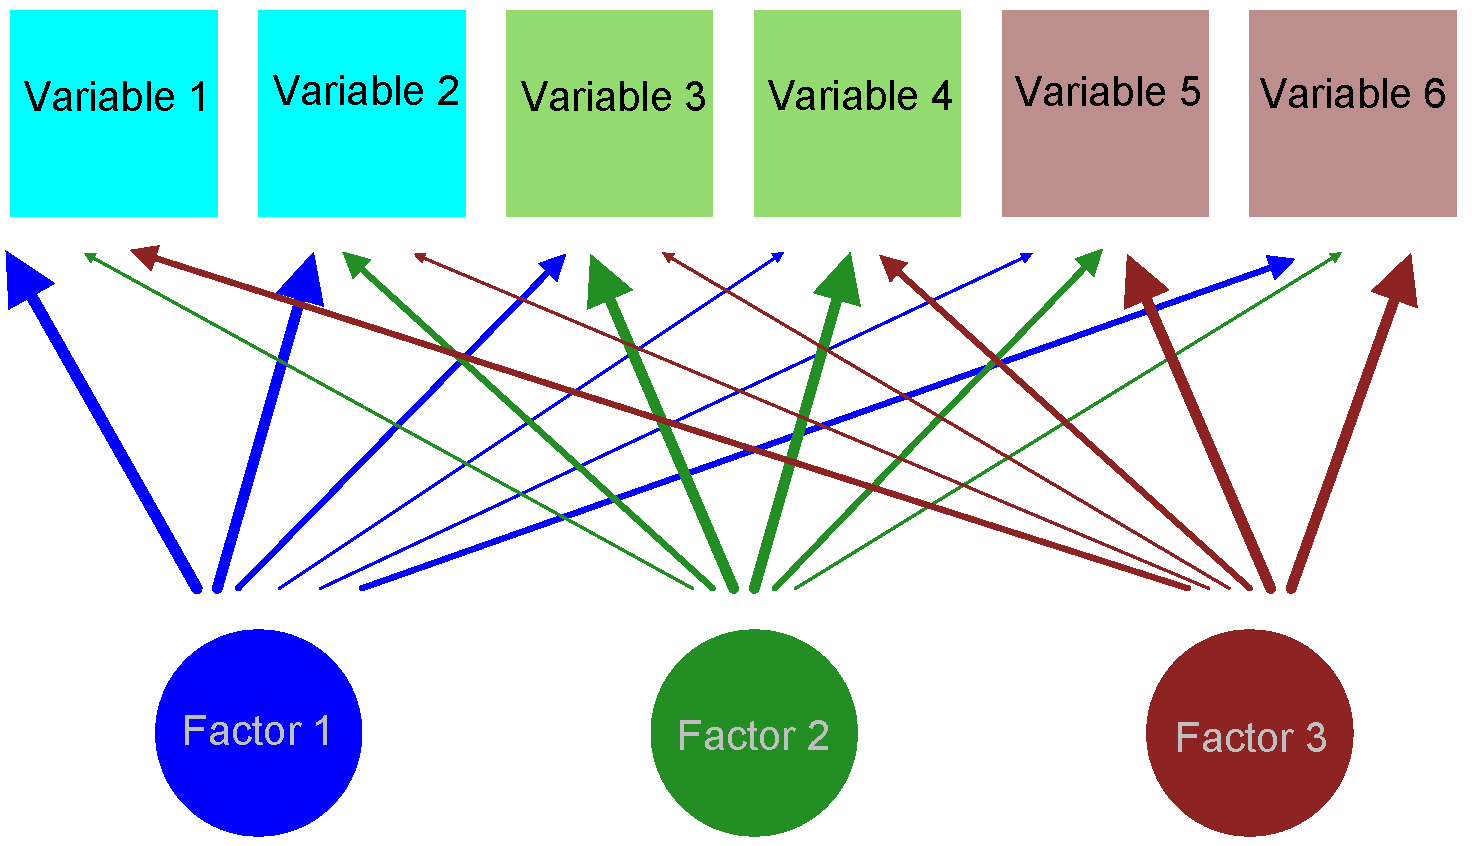
\includegraphics[width=0.75\textwidth]{Graphics/Variable-Factor}
\end{figure}

The following sources may offer additional help: \parencite{Hop-75,Wil-10,Klo-10,Fae-16,Fri-17}. If two observed variables \AbsVec{x, y} are correlated, then a change in a third, underlying (confounding), latent (unobserved) variable (\textbf{factor}) may be the cause (see fig. \ref{fig:VarFac}). Factor analysis is used to uncover such factors from an observed data set:
\begin{equation}
     z_{i,j} = \psi_{i,j} + \sum\limits_{k=1}^p \arr{L}_{j,k} \arr{C}_{i,k}
\end{equation}
with:
\begin{description}
    \item[\( z_{i,j} \)]{result of person \skalar{i} on item \skalar{j}, in standard deviations from mean}
    \item[\( \psi_{i,j} \)]{measurement error of person \skalar{i} on item \skalar{j}}
    \item[\( \arr{L}_{j,k} \)]{loading of factor \skalar{k} on variable \skalar{j}, that is, the correlation of \skalar{\AbsVec{F}_{j,k}} with variable \skalar{j} }
    \item[\( \arr{C}_{i,k} \)]{factor score of student \skalar{i} on factor \skalar{k} (\( \bar{\arr{C}} = 0, \sigma_\arr{C} = 1 \))}
\end{description}
The number of latent factors \skalar{p} is initially equal to the number of observed variables. However, often only a small number \skalar{q} of the factors is significant. The \textbf{eigenvalue} for each factor is the sum of the squared loadings of a factor on all variables. It explains how much of the  variance \skalar{\sigma} in the data is explained by that factor (column sum to the loading matrix). The data are usually \skalar{z}-standardised and hence have a variance of \skalar{1.0}. An eigenvalue of \num{1.0} therefore means that the factor explains as much variance as an observed variable. The ratio of eigenvalues is ratio of explanatory power of two factors. One can therefore use only those factors with significant eigenvalues, the reminder are thought to originate from experimental noise. The \textbf{communalities} \AbsVec{H} are the sum of the squared loadings of a variable over all factors (row sum of the squared loading matrix). It is the proportion of variance of the variable that can be explained by the factors. In the literature one may find the \textbf{uniqueness} instead, which is the 1 -- \AbsVec{H}.

The differences between Factor analysis and principle component analysis are:
\begin{itemize}
  \item{\acs{PCA} produces components, \acs{FA} factors. Components are a linear combination of observed variables, variables are a linear combination of the underlying factors.}
  \item{\acs{PCA} assumes that the data matrix is error free (all diagonal elements of the correlation matrix are unity), the components therefore contain error and are therefore not equal to latent variables (they are not necessarily interpretable). In \acs{FA} the data are assumed to contain error (diagonal elements of the correlation matrix contain communalities), and the factors extracted contain only the common variance (variance shared with other variables), but not the unique variance (variance specific to a particular variable, which is taken as error term). As a result, the correlation matrix is reconstructed by the components, but only approximated by the factors.}
  \item{\acs{PCA} is used to describe empirical data in causal modelling and to reduce the number of dimensions to ease further analysis (\Foreign{e.g.}, by cluster analysis or multidimensional regression). \acs{FA} is used to theoretically explore the underlying factor structure.}
  \item{In fig. \ref{fig:VarFac} the arrows have opposite direction for \acs{PCA}.}
  \item{\acs{PCA} tries to explain as much as possible of the variance of the variables (\( \sum_{i=1}^p{\AbsVec{s}_{ii}} \)) by reducing the elements of \arr{R} near the diagonal. \acs{FA} tries to account for the covariance between variables (\( \sum_{i,j=1}^p{\AbsVec{s}_{ij}}, i \neq j \)) by reducing the elements far from the diagonal. However, since the one cannot be achieved without the other, both methods do in practice nearly the same thing. }
\end{itemize}
The communality is the variance a variable shares with all other variables. With a high enough number of variables and subjects, the method used seems to have little impact on the results obtained (at least if the communalities are \(> 0.4 \)), so \acs{PCA} is the method of choice when there is no specific reason to use another (\parencite{Wil-10}, but see also \parencite{Cos-05} for a different opinion).

\section{Is a data set suitable for factor analysis and \acs{PCA}?}

\subsection{Number of data}

There are several criteria available. As a rule of thumb \parencite{Wil-10}, there should be at least 6, better more (up to 20 has been suggested) subjects per variable, so if 100 variables are studied, 600 subjects are required, 2000 would be ideal. Each factor should have a chance to be represented by several variables, for most studies that means that there should be \(> 30 \) variables.

The sampling density (average distance between data points) is proportional to \(n^\frac{1}{p} \), thus the number of samples \skalar{n} required for a reasonable representation of the data space increases rapidly with \skalar{p}.

\subsection{Correlation coefficients}

Most (off-diagonal) correlation coefficients should be \(0.3 < r < 0.8 \), with around \num{0.5} being ideal.

\subsection{Multivariate normality of data}\label{text:MulNorm}

Both \acs{FA} and \acs{PCA} require that the data are distributed multivariate normal, that is, every linear combination of its \skalar{p} components has a univariate normal distribution (\( ax_{\cdot i} + bx_{\cdot j} \) is normally distributed \(\forall\enspace i,j \in [1\ldots p] \) and \(a,b \in \set{R} \)). \parencite{Zyg-14} recommends the procedures in \parencite{Roy-95} (FORTAN-code available in \parencite{Mil-04}) and \parencite{Hen-90} to test this, both are available in the R-package MVN \parencite{Kor-14}. It is also possible to test for normality of each variable, this must be true if multivariate normality is true. Note, however, that normality of the individual data is necessary but not sufficient for multivariate normality of the entire set (see for example fig. \ref{fig:MultNorm} on page \pageref{fig:MultNorm}).

\subsection{The \Name{Kaiser-Meyer-Olkin} (KMO) criterium}

\begin{table}
  \caption{Interpretation of MSA-values according to \parencite{Kai-74}}
  \label{tab:KMO}
  \centering
    \begin{tabular}{ll}
      \toprule
      KMO        & Suitability \\
      \midrule
 \(> \) 0.90   & marvellous  \\
      0.80..0.90 & meritorious \\
      0.70..0.89 & middling    \\
      0.60..0.69 & mediocre    \\
      0.50..0.59 & miserable   \\
 \(< \) 0.50   & unacceptable\\
      \bottomrule
    \end{tabular}
\end{table}

For a correlation matrix \skalar{r} to be useful for factor analysis, \(\skalar{r}^{-1} \) should be near diagonal.
The KMO-criterium measures how close \(\skalar{r}^{-1} \) is to being diagonal:
\begin{equation}
  \mathrm{KMO} = \frac{\sum_{i=1}^{n}{\sum_{j=1}^{n}{r^2_{ij}}}}{\sum_{i=1}^{n}{\sum_{j=1}^{n}{r^2_{ij}}} +
  \sum_{i=1}^{n}{\sum_{j=1}^{n}{q^2_{ij}}}}, \qquad i \neq j
\end{equation}
with \skalar{r_{ij}} the correlation of variables \skalar{i} and \skalar{j} and \skalar{p_{ij}} the partial
correlation \parencite{Cer-77}:
\begin{align}
  \AbsVec{Q} &= \AbsVec{D} \skalar{r}^{-1} \AbsVec{D} \\
  \AbsVec{D} &= [(\diag{\skalar{r}^{-1}})^{1/2}]^{-1}
\end{align}
A large partial correlation means that the correlation matrix has little common variance and results in a small
KMO-value (see table \ref{tab:KMO}). It is also possible to use the \textbf{measure of sampling adequacy (MSA)} to
determine whether a particular variable \skalar{j} should be included in the analysis:
\begin{equation}
  \mathrm{MSA}_j = \frac{\sum_{i \neq j}{r^2_{ij}}}{\sum_{i \neq j}{r^2_{ij}} + \sum_{i \neq j}{q^2_{ij}}}
\end{equation}
If variables with a poor MSA are removed from the analysis, the overall KMO increases.

However, as shown by \parencite[p. 147]{Ren-02}, MSA is affected not only by the quality of \skalar{r}, but also
decreases with the number of significant factors. It therefore is of limited value.

\subsection{\Name{Bartlett}'s sphere test}

Tests \(H_0: \skalar{r} = \AbsVec{I} \) (the identity matrix) \Foreign{vs} \(H_1: \skalar{r} \neq \AbsVec{I} \)  \parencite{Bar-51}. If \(H_0 \) were true then there is no covariance between data, and the data points form a perfect sphere in \skalar{p}-dimensional space. Then of course there would be no principal component, all eigenvalues are identical except for noise.
\begin{align}
  \chi^2 &\approx -\left[(n-1)-\frac{2p+5}{6}\right] \times \log(||\arr{R}||) \\
  f      &= \frac{p(p-1)}{2}
\end{align}
with \skalar{||\arr{R}||} the determinant of the correlation matrix (which would be unity if \skalar{r} =
\AbsVec{I}). The correlation matrix is suitable if \(P_0 < \SI{5}{\%} \). The test is sensitive to deviation of the
data from multivariate normal distribution, which may lead to false acceptance of \(H_0 \).

\Name{Bartlett}'s test compares the volume of the data ellipsoid with the volume of the spheroid that would result if all axes were identical.  Another way to calculate \(\chi^2 \) is via the ratio between the geometric and arithmetic mean of all eigenvalues of the correlation matrix (which would be unity if the data were spherical):
\begin{align} \label{eqn:Bart}
  r      &= \frac{\tilde{\lambda}}{\bar{\lambda}} = \frac{\sqrt[p-k]{\prod_{i=k+1}^{p}{\lambda_i}}}{\frac{1}{p-k} \sum_{i=k+1}^{p}{\lambda_i}} \\
  \chi^2 &= -(n - (p-k) - 0.5) \times \ln(r^{p-k}) \notag \\
  f      &= \frac{(p - k - 2)(p - k - 1)}{2} \notag
\end{align}
with \skalar{k} the number of eigenvalues excluded from the analysis (in this context 0, but see eqn. \ref{eqn:BartNo}, where this becomes important).

\begin{lstlisting}[caption=\Name{Bartlett}'s sphere test]
  function Bartlett (const Cor : MatrixTyp; Cases : word) : float;

  var f, Variables  : word;
      chi2, Det, P0 : extended;

  begin
    Variables := MatrixRows(Cor);
    Det := Determinante(Cor);
    write('Determinante = ', det:10, ' ');
    chi2 := -(pred(Cases) - (2 * Variables + 5) / 6) * log(Det, 10);
    f := round(Variables * pred(Variables) / 2);
    write('chi2 := ', chi2:5:3, ' ', 'f = ', f:5, ' ');
    P0 := IntegralChi(chi2, f); // should be larger than 0.95
    writeln('P0 = ', (100*P0):3:1, '%');
    Bartlett := P0;
  end;
\end{lstlisting}

\section{Mathematical basis of principle component analysis}

\begin{figure}
   \caption{Geometrical interpretation of PCA, for a two-dimensional variable set. Each attribute carrier is
   represented by a (\emph{red}) dot in the \(\AbsVec{x}_1, \AbsVec{x}_2 \)-plane. All data form an ellipsoid cloud,
   with the ellipsoid representing a surface of identical density. Transformation occurs by centering the
   ellipsoid (subtracting the vector of averages \(\bar{\AbsVec{x}}_1, \bar{\AbsVec{x}}_2, \ldots
   \bar{\AbsVec{x}}_p \), \emph{purple}) and rotating the coordinate system so that the first principal component
   (\emph{green}) is the largest radius of that ellipsoid, the eigenvalue is the length of this vector. The second
   principal component is orthogonal to the first, and represents the second-largest radius of the ellipsoid, and
   so on for higher dimensions. }
   \label{fig:PCA-geo}
   \centering
      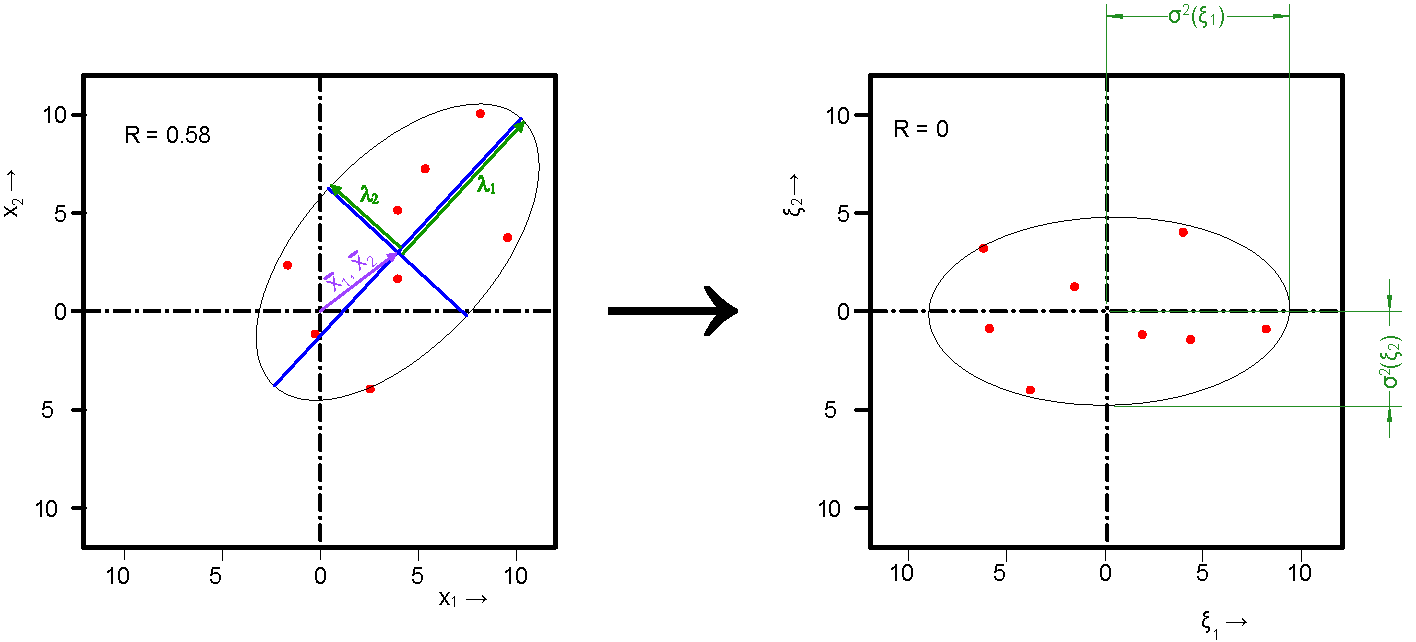
\includegraphics[width=\textwidth]{Graphics/PCA}
\end{figure}

\begin{figure}
   \caption{Distance of a point to the regression line (\emph{green, left}) and the principle component (\textit{purple, right}) for the 2D case. In linear regression, the independent variable \skalar{x} is assumed to be error free, and the distance of a data point to the regression line is measured in the direction of the dependent variable \skalar{y} (orthogonal to the \skalar{x}-axis). In \acs{PCA} all variables are equivalent, measurements for each individual have errors in both \skalar{x}- and \skalar{y}-direction. The distance of the data point to the principle component is orthogonal to that component (as in \Name{Deming}-regression with \(\sigma = 1 \), see section \ref{sec:Deming} on page \pageref{sec:Deming}). }
   \label{fig:DirDist}
   \centering
      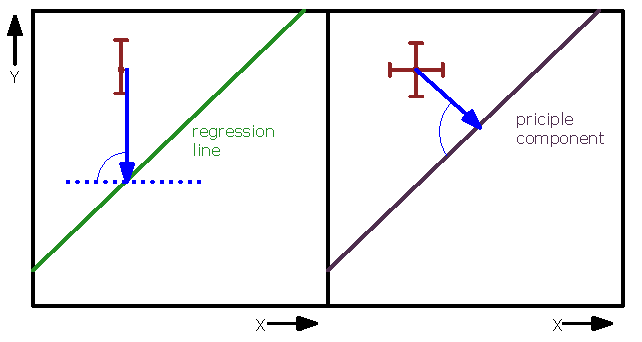
\includegraphics[width=0.75\textwidth]{Graphics/DirectionOfDistance}
\end{figure}

\begin{figure}
   \caption{There is only one direction of the principle axis that maximises the spread of the projection of the data (variance), in this position the distance of the data points from the axis is minimal. Data points in blue, projections in red.  One can think of the distances as springs, which apply a force onto the principle component according to \Name{Hooke}'s law. Then the component will orient itself so that the overall force is zero. Figure from \href{https://stats.stackexchange.com/questions/2691/making-sense-of-principal-component-analysis-eigenvectors-eigenvalues?rq=1}{https://stats.stackexchange.com/questions/2691/making-sense-of-principal-component-analysis-eigenvectors-eigenvalues?rq=1}. }
   \label{fig:MaxVar}
   \centering
   \includemedia[
       label=,
       width=\linewidth,height=0.4\linewidth,
       addresource=AxisRotation.flv,
       transparent, %transparent player background
       activate=pageopen,
       passcontext, %show VPlayer’s rightclick menu
       flashvars={
          source=AxisRotation.flv
          &loop=true
       }
       ]{}{VPlayer.swf}
\end{figure}

PCA was invented by \Name{Hotelling} \parencite{Hot-33}, using the work of several authors. The data in a data matrix \AbsVec{X} can be interpreted as points in a \skalar{p}-dimensional cloud (see fig. \ref{fig:PCA-geo}). The data points are enveloped by an ellipsoid (ellipse in the two-dimensional case), which represents a surface of equal density.

The first principle component is, in effect, a kind of regression line through the data cloud (actually, linear regression minimises the distances from the regression line as measured orthogonal to the \skalar{x}-axis, in \acs{PCA} they are measured orthogonal to the component, see fig. \ref{fig:DirDist}). If we calculate the distance of all data points from the regression line, the second principle component would be a regression through those, and so on. The first component coincides with the major axis of the ellipsoid. This vector has \skalar{p} elements and is called an \emph{eigenvector}. In \Name{Euklid}ian space, the length of a vector is the root of the sum of the squares of the elements (see eqn. \ref{fig:PCA-geo}), this length is called \emph{eigenvalue}.

For the data matrix a variance-covariance matrix \(\arr{S} = \AbsVec{X}^T\AbsVec{X} / (p-1) \) (if the data are z-standardised, otherwise the correlation matrix \(\arr{R} \) is used) is calculated.

Aside: Interconversion of \arr{S} and \arr{R}: \(\skalar{r}_{ij} = \frac{\AbsVec{s}_{ij}}{\AbsVec{s}_i \AbsVec{s}_j} \). Hence if \(\arr{A} = \diag(\AbsVec{s}_1, \AbsVec{s}_2, ... , \AbsVec{s}_p) \) a diagonal matrix of variances, then \(\arr{S} = \arr{A}\arr{R}\arr{A} \) is the variance-covariance matrix and and \(\arr{R} = \arr{A}^{-1} \arr{S} \arr{A}^{-1} \).

The sum of squares for both data vectors in the example is \num{500}. For this purpose the data matrix \(\AbsVec{X}_{n \times p} \) is multiplied with a weight matrix \(\AbsVec{F} \), resulting in a factor score matrix \arr{C}: \(\arr{C} = \AbsVec{X} \AbsVec{F} \). Then the sums of squares (= eigenvalues) are now differently distributed (\num{400} and \num{100} instead of \num{208} and \num{292}, respectively), but their sum is the same. Also, the correlation between \(\AbsVec{c}_1 \) and \(\AbsVec{c}_2 \) is now \num{0}, the components are independent. The eigenvalues are arranged in a diagonal matrix \(\Lambda \):
\begin{gather}
   \Lambda = \begin{pmatrix} \lambda_1 & 0 \\ 0 & \lambda_2 \end{pmatrix} =
  \begin{pmatrix} 400 & 0 \\ 0 & 100 \end{pmatrix}
\end{gather}
\AbsVec{F} represents tests, \arr{C} persons, \(\AbsVec{X} = \arr{C} \AbsVec{F}' \).

How do we get \(\Lambda \)? From the \emph{characteristic equation}:
\begin{equation}
  ||\arr{S} - \lambda_i \arr{I}|| = 0
\end{equation}
with \(||\ || \) the determinant and \arr{I} the identity matrix (all diagonal elements 1, all other elements 0).
Thus, in our example the determinant of:
\begin{gather}
  \begin{pmatrix} 208 & 144 \\ 144 & 292 \end{pmatrix} -\lambda_i
  \begin{pmatrix} 1 & 0 \\ 0 & 1 \end{pmatrix} =
  \begin{pmatrix} 208-\lambda_i & 144-0 \\ 144-0 & 292-\lambda_i \end{pmatrix}
\end{gather}
This leads to
\begin{equation}
  \lambda_i^2 - 500 \lambda_i + \num{40000} = 0
\end{equation}
which, when solved for \(\lambda_i \) gives (\num{400}, \num{100}). For each \(\lambda_i \) we can calculate the
corresponding latent vector \(\AbsVec{f}_i \) from
\begin{equation}
  (\arr{S} - \lambda_i \arr{I}) \AbsVec{f}_i = 0
\end{equation}
which is for \(\AbsVec{l}_1 = 400 \):
\begin{gather}
   \left[ \begin{pmatrix} 208 & 144 \\ 144 & 292 \end{pmatrix} - 400
   \begin{pmatrix} 1 & 0 \\ 0 & 1 \end{pmatrix} \right]
   \begin{pmatrix} 0.6 \\ 0.8 \end{pmatrix}  =
   \begin{pmatrix} -192 & 144 \\ 144 & -108 \end{pmatrix}
   \begin{pmatrix} 0.6 \\ 0.8 \end{pmatrix} =
   \begin{pmatrix} 0 \\ 0 \end{pmatrix}
\end{gather}

Where do the equations
\begin{equation}
  ||\arr{S} - \lambda_i \arr{I}|| = 0 \quad (\arr{S} - \lambda_i \arr{I}) \AbsVec{f}_i = 0
\end{equation}
come from?  If a vector \AbsVec{X} is left-multiplied with an array \arr{A}, another vector \AbsVec{Y} is
obtained, which is called a transformation of \AbsVec{X}: \(\arr{A} \AbsVec{X} = \AbsVec{Y} \). In the case of PCA,
\AbsVec{X} maintains its direction, in our example: \( \arr{S} \AbsVec{F} = \lambda_i \AbsVec{F} \). This is equivalent
to
\begin{equation}
  \arr{S} \AbsVec{F} - \lambda_i \AbsVec{F} = 0 = (\arr{S} - \lambda_i \arr{I}) \AbsVec{F}
\end{equation}
Unless the determinant \(||\arr{S} - \lambda_i \arr{I}|| = 0 \) the vector \(\AbsVec{F} \) will be 0.

Considering fig. \ref{fig:PCA-geo}, there are a few points on the ellipse where the normal of the tangent has the
same direction as the line connecting the point to the focus of the ellipse. This identity determines a latent
vector.

To do a \acs{PCA} perform the following steps:
\begin{enumerate}
  \item{Arrange data in a matrix with persons in rows and variables in columns (\( \AbsVec{X}_{n \times p} \)). }
  \item{Calculate the arithmetic means and standard deviation of all variables of \AbsVec{X} (that is, of all columns).}
  \item{Center the data by subtracting the column means from all columns.}
  \item{From the centered data matrix \arr{X} calculate the variance-covariance matrix \arr{S}, \(\AbsVec{s}_{i,j} = \frac{\sum_{k=1}^{n}{(\AbsVec{x}_{k,i}-\bar{\AbsVec{x}}_i)} \times \sum_{k=1}^{n}{(\AbsVec{x}_{k,j}-\bar{\AbsVec{x}}_j)}}{n-1} \) or the
      correlation matrix \arr{R}. The variance-covariance matrix may also be calculated by \(\arr{S} = \arr{X}^T\arr{X}/(p-1) \), the correlation matrix from \(\arr{R} = \arr{Z}^T\arr{Z} \).}
  \item{Perform an eigenanalysis of either matrix, resulting in the diagonal matrix of eigenvalues \(\Lambda \) and the corresponding eigenvectors (components) \(\arr{E}_{p \times p} \). Note that using \arr{R} or \arr{S} will yield different results unless the data matrix is not only centered, but \skalar{z}-standardised.}
  \item{Calculate the  proportion of explained variance by dividing each eigenvalue \(\lambda_i \) by the sum of
      all eigenvalues \(\sum_{j=1}^p{\lambda_i} = p \), and its cumulative sum.}
  \item{Calculate the acceleration \(f''(j) \approx (f(j+1) - 2f(j) + f(j-1)) \), the second derivative of the scree-plot}
  \item{Calculate the product of the eigenvalues \(\prod_{i=1}^p \lambda_i = ||\arr{R}|| \) required for the sphericity test (see above).}
  \item{Generate the diagonal matrix \skalar{\Lambda} with eigenvalues on the diagonal. This is the variance-covariance of the components. }
  \item{Determine the number of significant eigenvalues \skalar{q}, and keep the corresponding
      eigenvectors in a projection matrix \(\arr{F}_{p \times q} \) column-wise from left to right.}
  \item{Calculate the factor score matrix (principle components) by \(\arr{C}_{n \times q}^T = \arr{X}_{n \times p} \arr{F}_{p \times q} \). }
  \item{Calculate the correlation between variables and factors, the \textbf{loadings} \(\arr{L}_{p \times
      q} \). This is the proportion of variance in a variable that is accounted for by a factor. For each variable, the \textbf{communality}, is calculated as \[\AbsVec{h}_j = \sum_{k=1}^{q}{\AbsVec{l}_{j,k}^2}\], the row sum of squared loadings. Sometimes, in the literature the \textbf{uniqueness}  = \( 1 - \AbsVec{h}_j \) is used instead.}
  \item{Likewise, the column sum of squared loadings is the \textbf{sum of squared loadings}. The SSLoadings divided by its total is \textbf{variance accounted for}. }
  \item{\Name{Hoffman}'s index of complexity \parencite{Hof-77} for each item is \(\frac{(\sum_{k=1}^{q}{l_{jk}^2})^2}{\sum_{j=1}^{q}{l_{j k}^4}} \). }
  \item{If \acs{PCA} is used as a method of factor analysis, identify for each factor the \(\approx \) \num{5} variables that have the highest and lowest correlation and use these to interpret the factors. }
  \item{A rotation of the coordinate system can be tried to obtain more interpretable components. In that case, the scores have to be recalculated to match the rotated loadings. In this case, one should no longer speak of ``principal components'', but of ``rotated components''.}
\end{enumerate}

Asside: \acs{PCA} can also be performed using singular value decomposition on the centered data matrix (\( \arr{X}_{n \times p} = \arr{P}_{n \times p} \Delta_{p \times p} \arr{Q}_{p \times p}^T \)). Columns of  \arr{P} contain the left singular vectors, and \(\arr{F} = \arr{P} \Delta \). These singular vectors are the normalised eigenvectors of \(\arr{X}\arr{X}^T \). Columns of the loading matrix \arr{Q} contain the of right singular vectors, and \arr{X}\arr{Q} gives the projections of data onto the principal components. The vectors in \arr{Q} are the normalised eigenvalues of \(\arr{X}^T \arr{X} \). The diagonal matrix \(\Delta \) contains the singular values and is related to eigenvalues by \(\lambda_i = \delta^2_i \), where \(\Lambda \) contains the eigenvalues of both \(\arr{X}\arr{X}^T \) and \(\arr{X}^T \arr{X} \), which are identical.

The \textbf{non-linear iterative partial least squares (NIPALS)} algorithm calculates the first eigenvector and the first score column of a data matrix, their outer product is subtracted from the data matrix, the resulting residual matrix is used to calculate the second eigenvector/loading vector and so on. With very large data sets (\Foreign{e.g.}, in -omics), which have only a few significant components, this can lead to significant savings in computer time, however, the algorithm is sensitive to roundoff and cancellation errors.

\subsection{Calculation of component and factor scores}

Once the loading matrix \arr{L} has been calculated and -- if desired -- rotated, the next step is the calculation of the scores each individual has on the \skalar{q} relevant factors. As these scores are free of co-linearity, they can be used as variables for further analysis, for example regression or cluster analysis. The dimension of the score matrix \arr{C} is \skalar{n\times q}. For this purpose, a matrix of regression coefficients $\arr{A}_{p\times q}$ is calculated, then  \arr{C} = \arr{XA} or, better, \arr{ZA} if the correlation matrix or the centered values of \arr{X} if the covariance matrix was used. The regression matrix may be saved and used to calculate scores for new observations. The scores calculated have a variance of unity (or nearly so). There are several methods to calculate \arr{A} \parencite{ttn-14}:

\subsubsection{The coarse (\Name{Cattell}'s) method}

\( \arr{A} = \arr{L}\). The data matrix \arr{X} should be centered (if the covariance-matrix \arr{S} was used to calculate \arr{L}) or \skalar{z}-standardised (if \arr{R} was used). It is possible to set low values of \arr{A} to zero, or even to dichotomise all elements of \arr{L} to either zero or unity. The main value of this method used to be that it does not require matrix inversion and hence is computationally cheap, but with the increased power of personal computers that is no longer an issue. Score values also tend to be more stable from sample to sample if sampling is not ideal, the coarse method is hence used mainly in exploratory analysis, where the reliability and validity of the factors has not yet been tested.

\subsubsection{The refined methods}

After unrotated PCA one can simply use \( \arr{A} = \arr{L} \Lambda^{-1} = \arr{R}^{-1} \arr{L} \), that is, each column of \arr{L} is divided (scaled) by the corresponding eigenvalue. The method results in scores that have a variance of unity. If rotation was performed, \( \arr{A} = (\arr{L}^+)^T \), the transposed pseudoinverse.

After factor analysis several methods are available, including:
\begin{description}
  \item[Regression method]{\parencite{Tom-35,Thu-35} \(\arr{A} = \arr{R}^{-1} \arr{LI} \). This formula may also be used in PCA (and is the only method available in SPSS after PCA extraction).}
  \item[\Name{Horst}'s method]{\parencite{Hor-65} \(\arr{A} = \arr{LL}^T\arr{LI} = (\arr{L}^+)^T \). }
  \item[\Name{Anderson-Rubin}'s method]{\(\arr{A} = \arr{L}^T\arr{U}^{-1} \arr{R} \arr{U}^{-1} \arr{L} \). The scores have a variance of exactly one. This method can be used only after orthogonal, not oblique, rotations.}
  \item[\Name{McDonald-Anderson-Rubin}'s method]{\(\arr{A} = \arr{R}^{1/2} \arr{GH}^T \arr{I}^{1/2} \), where \( \svd(\arr{R}^{1/2} \arr{U}^{-1} \arr{L} \arr{I}^{1/2}) = \arr{G}\Delta\arr{H}^T \). This method is an extension of {Anderson-Rubin}'s method that works after both orthogonal and oblique rotations.  }
  \item[\Name{Green}'s method]{is a modification of \Name{McDonald-Anderson-Rubin}'s method, where \( \svd(\arr{R}^{1/2} \arr{L} \arr{I}^{3/2}) = \arr{G}\Delta\arr{H}^T \). This method may also be used after PCA, giving the same result as \Name{Horst}'s.}
\end{description}

\section{Pascal program for PCA}

The main program then is as follows:
\begin{lstlisting}[caption=Main program for PCA]
  PROGRAM Principal;

  USES
    Math,              // Lazarus math UNIT
    mathfunc,          // basic mathematical routines FOR real AND INTEGER
    Complex,           // routines FOR complex numbers
    Vector,            // vector algebra
    Matrix,            // basic matrix algebra
    stat,              // statistical TEST distributions
    Correlations,      // various types OF correlation coefficients
    PCA,               // principal component analysis
    PerformShrinkage,  // Ledoit-Wolf shrinkage OF correlation matrix
    Rotation,          // rotation OF loading matrix
    SystemSolve,       // linear equations
    EigenValues,       // calculation OF eigenvalues
    Zufall;            // generate Random numbers

  VAR
    Types                                                : TypeVector;
    EV, Variance, CumVariance, ImputVector, Acc,
    Communalities, Uniqueness, VarianceAccounted         : VectorTyp;
    Data, Cor, EigenVectoren, Scores, Identity, Loadings : MatrixTyp;
    Freqs                                                : FreqsType;
    x                                                    : float;
    Cases, i, iter                                       : WORD;


  BEGIN
    ProblemName := 'Anonym';
    SigVecs := 40;
    ReadCSV(Types, Data);
    CalculateCorrelationMatrix(Data, Types, Cor);
    WriteCorrelations(Cor, FALSE);
    Cases := MatrixRows(Data);
    Average(Cor, 0.5);               // perform shrinkage by average correlation
    WriteCorrelations(Cor, TRUE);
    AnalyseFrequencies(Cor, Types, Freqs);
    WriteCorrelations(Cor, TRUE);
    x := Bartlett(Cor, Cases);
    i := Jacobi(Cor, EV, EigenVectoren, Iter); // eigenanalysis
    Writeln('Jacobi: ', Iter: 3, ' iterations, Result = ', i:2, ': ', EigenError[i]);
    DestroyMatrix(Cor);
    SortEigenValues(EV, EigenVectoren);
    ExplainedVariance(EV, Acc, Variance, CumVariance);
    WriteEigenVector(EigenVectoren);
    Writeln('Eigenvectors and -values written');
    MaximumLikelihood(Data, Types, ImputVector);       // Scores
    RobustProduct(Data, EigenVectoren, ImputVector, Scores);
    WriteComponentScores(Scores);
    Writeln('scores written');
    CalculateLoadings(Data, Scores, Types, Loadings);  // unrotated Loadings
    CalculateCommunalities(Loadings, Communalities, Uniqueness, VarianceAccounted);
    WriteLoadings(Loadings, Communalities, Uniqueness, VarianceAccounted, FALSE);
    Writeln('Loadings and communalities calculated and written');
    DestroyVector(Variance);
    DestroyVector(CumVariance);
    DestroyVector(Communalities);
    CreateIdentityMatrix(Identity, SigVecs);
    GradProjAlgOrth(Loadings, Identity, Varimax);      // rotation
    CalculateCommunalities(Loadings, Communalities, Uniqueness, VarianceAccounted);
    WriteLoadings(Loadings, Communalities, Uniqueness, VarianceAccounted, TRUE);
    DestroyMatrix(Identity);
    DestroyMatrix(Data);
    DestroyMatrix(EigenVectoren);
    DestroyMatrix(Scores);
    DestroyMatrix(Loadings);
    DestroyVector(EV);
    DestroyVector(ImputVector);
    DestroyVector(Communalities);
    Writeln('All done, press <CR> to finish:');
    ReadLn;
  END.
\end{lstlisting}

The actual beef is in units \texttt{PCA, PerformShrinkage} and \texttt{Rotation}.

\section{Example: Phylogentic trees from nucleic acid sequences}

All life on earth is thought to originate from a single primordial Archaea-like cell that arose about \num{3.5e9} years ago. This common origin is reflected by sequence similarities in the sequences of common genes. More closely related species have more similar sequences than species whose last common ancestor lived long ago. Thus, it is possible to derive the \emph{tree of life} from sequence comparison, this is a task of bioinformatics.

Usually, sequences are compared by aligning them and then counting differences (insertions, delitions, mutations). However, multiple sequence alignment is computationally expensive, the problem is NP-complete. There are heuristic solutions to the problem implemented in programs like \texttt{Clustal} \parencite{Lar-07} or \texttt{MUSCLE} \parencite{Edg-04}.

\begin{figure}
 \caption{\capstart Phylogenetic tree of Corona- and Lentivirus, using nucleic acid word frequencies (word length = \num{4}). The first principal component of that matrix corresponds to the virus family, the second to similarity within a family. These principal components are sufficient to calculate a distance matrix and a hierarchical tree that agrees well with our knowledge of virus evolution. Compared to \texttt{Clustal}, which required almost \SI{4}{h} to calculate a similar tree by multiple sequence alignment, this calculation took only seconds. For details see text.}
   \label{fig:PincComp}
   \centering
     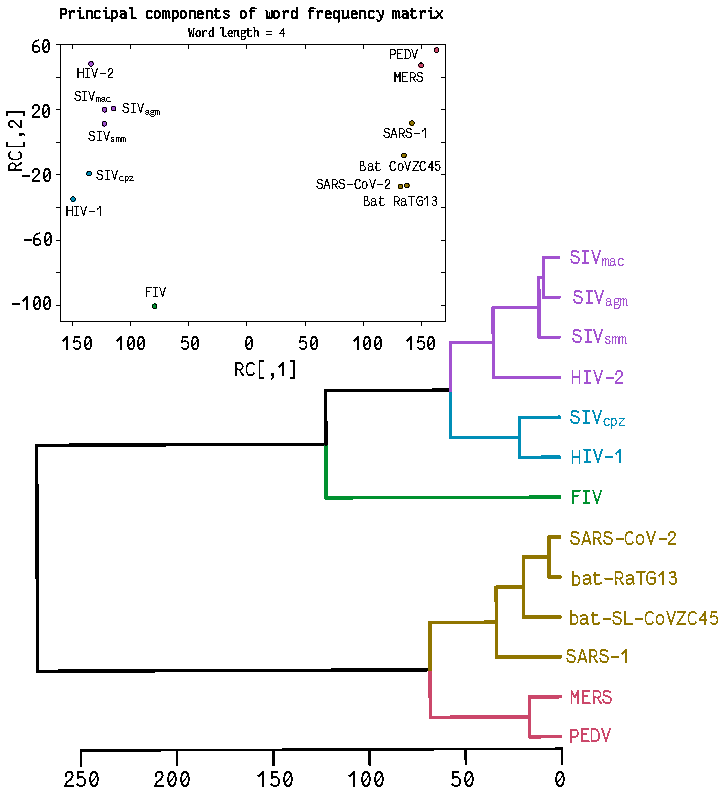
\includegraphics[width=0.75\textwidth]{Graphics/PrincComp}
\end{figure}

It has been shown that a lot of information about a nucleic acid sequence is contained in the word count \parencite{Bas-03,Hac-11}. For example, the sequence ``acg'' contains two words of length two: ``ac'' and ``cg''. Thus, the result of this operation is a 2D data matrix with \skalar{n} rows (\acs{OTU}s) and the possible words (\num{16}, \num{64}, \num{256}, \num{1024}, for word lengths of \num{2}, \num{3}, \num{4}, \num{5}, respectively) in columns. To avoid too many empty cells, word length should be \( < \log_4(m) \), where \skalar{m} is the sequence length. The resulting frequency table can be either used directly to calculate a distance matrix, or subjected to \acs{PCA} first. In the latter case, the first two principal components are sufficient for clustering (see fig. ref{fig:PincComp}).


     % -*- TeX:UK -*-
\section{The unit PCA}

The unit \acs{PCA} contains routines used by the program \texttt{Principal}. The interface is

\begin{lstlisting}[caption=Interface of unit PCA]
  UNIT PCA;

  { Performs routines in the context of principle component analysis }

  INTERFACE

  USES Math, Mathfunc, Stat, Correlations, Vector, Matrix;

  CONST
    MaxVariables = 180;
    SepChar = ';';
    // IN Middle Europe variables IN CSV separated by ";" AS "," IS decimal separator
    SigVecs: WORD = 5;
    // number OF significant vectors, can be changed by calling PROGRAM
    ProblemName: STRING = ''; // first name OF all files produced;
    Border = 20;  // number OF ranges FOR statistical analysis OF correlations

  TYPE
    DataTypes = (binary, nominal, ordinal, interval, rational);
    TypeVector = ARRAY[1..MaxVariables] OF DataTypes;
    FreqsType = ARRAY[DataTypes, DataTypes, -Border..Border] OF WORD;


  PROCEDURE ReadCSV(VAR Types: TypeVector; VAR Data: MatrixTyp);
  { Read data from CSV file. }

  PROCEDURE CalculateCorrelationMatrix(CONST Data: MatrixTyp;
    CONST Types: TypeVector; VAR Cor: MatrixTyp);
  { calculates correlation matrix for a mixed type data matrix. NaN-values
    are handled. }

  PROCEDURE ReadCorrelations(VAR Cor: MatrixTyp);
  { If the correlation matrix has been calculated previously,
    read it from CSV file }

  PROCEDURE WriteCorrelations(CONST Cor: MatrixTyp; Shrunk: BOOLEAN);
  { Writes the correlation matrix into a csv-file. File name will depend on
    whether the matrix has been shrunk.}

  PROCEDURE AnalyseFrequencies(CONST Cor: MatrixTyp; CONST Types: TypeVector;
    VAR Freqs: FreqsType);
  { Determine distribution of correlation coefficients by variable type }

  FUNCTION Bartlett(CONST Cor: MatrixTyp; Cases: WORD): double;
  { Bartlett's test for sphericity }

  PROCEDURE ExplainedVariance(CONST EigenValues: VectorTyp;
    VAR Acc, Variance, CumVariance: VectorTyp);
  { calculate acceleration, explained variance and cumulative explained variance
    from eigenvalues and writes them into a csv-file }

  PROCEDURE WriteEigenVector(CONST EigenVectors: MatrixTyp);
  { writes eigenvectors into a csv-file }

  PROCEDURE MaximumLikelihood(CONST Data: MatrixTyp; CONST Types: TypeVector;
    VAR ImputVector: VectorTyp);
  { Determin average (cardinal) or most common (other) value of a column for
    imputation }

  PROCEDURE RobustProduct(CONST A, B: MatrixTyp; CONST ImputVector: VectorTyp;
    VAR C: MatrixTyp);
  { robust matrix product, elements of A (original data) may be NaN and are replaced
    by the j-th element in ImputVector. For B (Eigenvectors) this precaution is not
    necessary. Only the first Max eigenvectors are used. }

  PROCEDURE WriteComponentScores(CONST Scores: MatrixTyp);
  { writes component scores into a csv-file }

  PROCEDURE CalculateLoadings(CONST Data, Scores: MatrixTyp;
    CONST Types: TypeVector; VAR Loadings: MatrixTyp);

  PROCEDURE CalculateCommunalities(CONST Loadings: MatrixTyp;
    VAR Communalities, Uniqueness,
    VarianceAccounted: VectorTyp);
  { Row and column sums of squared loadings }

  PROCEDURE WriteLoadings(CONST Loadings: MatrixTyp;
    CONST Communalities, Uniqueness,
    VarianceAccounted: VectorTyp;
    Rotated: BOOLEAN);
  { Writes loadings into a csv-file. File name will depend on whether the
    loadings have been rotated. }

  IMPLEMENTATION

  VAR
    Significance: SignificanceType;
\end{lstlisting}

The following procedure reads data from a .csv-file, the first row contains the variable names, the second the variable level (nominal, ordinal, interval and rational). The routine can be used for files following both US- and European conventions for decimal indicator (./,) and separation character (,/;):

\begin{lstlisting}
  PROCEDURE ReadCorrelations(VAR Cor: MatrixTyp);
  // Read correlation matrix from CSV FILE

  VAR
    InputFile: TEXT;
    c: CHAR;
    s: STRING;
    Variables, Error, i, j: WORD;
    x: double;

  BEGIN
    Assign(InputFile, Problemname + '-NativeCorr.csv');
    Reset(InputFile);
    Variables := 0;
    WHILE NOT EoLn(InputFile) DO  // Read first Line WITH variable numbers, count Variables
      BEGIN   // nothing needs TO be done with these values
        INC(Variables);
        i := ReadInt(InputFile) ;
      END; { while }
    ReadLn(InputFile);            // go TO next Line
    DEC(Variables);               // Line number
    CreateMatrix(Cor, Variables, Variables, 0.0);
    FOR i := 1 TO Variables DO    // now Read data from following lines
      BEGIN
        j := ReadInt(InputFile);  // Line number
        FOR j := 1 TO Variables DO
          SetMatrixElement(Cor, i, j, ReadFloat(InputFile));   // values
        ReadLn(InputFile);
      END; { for i }
    Close(InputFile);
    Writeln(Variables: 3, ' variables read, ');
  END;
\end{lstlisting}

Calculating the correlation matrix can be time consuming. If this has been done already in the past, the following routine reads such a matrix from a file.

\begin{lstlisting}[caption=Read correlation matrix from a csv-file]
  PROCEDURE ReadCorrelations(VAR Cor: MatrixTyp);
  // Read correlation matrix from CSV FILE

  VAR
    InputFile: TEXT;
    c: CHAR;
    s: STRING;
    Variables, Error, i, j: WORD;
    x: double;

  BEGIN
    Assign(InputFile, Problemname + '-NativeCorr.csv');
    Reset(InputFile);
    Variables := 0;
    WHILE NOT EoLn(InputFile) DO  // Read first Line WITH variable numbers, count Variables
      BEGIN   // nothing needs TO be done with these values
        INC(Variables);
        i := ReadInt(InputFile) ;
      END; { while }
    ReadLn(InputFile);            // go TO next Line
    DEC(Variables);               // Line number
    CreateMatrix(Cor, Variables, Variables, 0.0);
    FOR i := 1 TO Variables DO    // now Read data from following lines
      BEGIN
        j := ReadInt(InputFile);  // Line number
        FOR j := 1 TO Variables DO
          SetMatrixElement(Cor, i, j, ReadFloat(InputFile));   // values
        ReadLn(InputFile);
      END; { for i }
    Close(InputFile);
    Writeln(Variables: 3, ' variables read, ');
  END;
\end{lstlisting}

The following routine analyses the distribution frequency for the values in \arr{R} and writes them to a file.

\begin{lstlisting}[caption=Determine frequency distribution of correlation coefficients]
  PROCEDURE AnalyseFrequencies(CONST Cor: MatrixTyp; CONST Types: TypeVector;
                               VAR Freqs: FreqsType);

  CONST
    TypeText: ARRAY [DataTypes] OF STRING[8] =
      ('binary', 'nominal', 'ordinal', 'interval', 'rational');

  VAR
    i, j: DataTypes;
    l, m, Variables: WORD;
    k: INTEGER;
    OutFile: TEXT;
    x: double;

  BEGIN
    Assign(OutFile, ProblemName + '-Frequencies.csv');
    Rewrite(OutFile);
    Variables := MatrixRows(Cor);
    FOR i := LOW(DataTypes) TO High(DataTypes) DO
      FOR j := LOW(DataTypes) TO High(DataTypes) DO
        FOR k := -Border TO Border DO
          Freqs[i, j, k] := 0;
    FOR l := 1 TO Variables DO
      FOR m := 1 TO Variables DO
        BEGIN
          x := GetMatrixElement(Cor, l, m) * Border;
          INC(Freqs[Types[l], Types[m], Round(x)]);
        END;
    FOR i := LOW(DataTypes) TO High(DataTypes) DO
      BEGIN
        Writeln(OutFile, TypeText[i]: 8, SepChar);
        FOR j := LOW(DataTypes) TO High(DataTypes) DO
          BEGIN
            Write(OutFile, SepChar, TypeText[j]: 8, SepChar);
            FOR k := -Border TO Border DO
              Write(OutFile, Freqs[i, j, k]: 4, SepChar);
            Writeln(OutFile);
          END;
      END;
    Close(OutFile);
  END;
\end{lstlisting}

The \texttt{procedure CalculateCorrelationMatrix} can calculate correlation coefficients appropriate for the levels of the data. In practice, it is often better to calculate \Name{Pearson}'s product moment correlation \skalar{r_p} for binary, ordinal, interval and rational data, and to avoid nominal data at all. This minimises rank deficiency of the correlation matrix. If that is all that is desired, the \texttt{case}-statement can be simplified accordingly.

\begin{lstlisting}[caption=Calculate the correlation matrix]
  PROCEDURE CalculateCorrelationMatrix(CONST Data: MatrixTyp;  CONST Types:
            TypeVector; VAR Cor: MatrixTyp);

  VAR
    i, j, Variables: WORD;
    IVector, JVector: VectorTyp;
    Rxy: double;
    Cont: ContTable;

  BEGIN
    Variables := MatrixColumns(Data);
    CreateIdentityMatrix(Cor, Variables);
    GetColumn(Data, i, IVector);
    for i := 1 to Variables do
      begin
        SetMatrixElement(Cor, i, i, 1.0);    // diagonal
        GetColumn(Data, i, IVector);
        FOR j := Succ(i) TO Variables DO
          BEGIN
            GetColumn(Data, j, JVector);
            CASE Types[i] OF
              nominal: CASE Types[j] OF
                        nominal:  BEGIN
                                    Contingency(IVector, JVector, Cont);
                                    Rxy := lambda(Cont);
                                    Rxy := sign(Rxy) * Sqrt(Abs(Rxy));
                                    DestroyContingency(Cont);
                                  END;
                        ordinal:  BEGIN
                                    Contingency(IVector, JVector, Cont);
                                    Rxy := theta(Cont);
                                    Rxy := Sqrt(Rxy);
                                    // asymmetric: only positive values!
                                    DestroyContingency(Cont);
                                  END;
                        binary:   BEGIN
                                    Contingency(IVector, JVector, Cont);
                                    Rxy := lambda(Cont);
                                    Rxy := sign(Rxy) * Sqrt(Abs(Rxy));
                                    DestroyContingency(Cont);
                                  END;
                        interval,
                        rational: BEGIN
                                    Rxy := eta_sqr(IVector, JVector, Significance);
                                    Rxy := Sqrt(Rxy);
                                    // asymmetric: only positive values!
                                  END;
                       END;
              ordinal: CASE Types[j] OF
                        nominal:  BEGIN
                                    Contingency(JVector, IVector, Cont);
                                    Rxy := theta(Cont);
                                    Rxy := Sqrt(Rxy);
                                    DestroyContingency(Cont);
                                  END;
                        ordinal:  BEGIN
                                    Rxy :=
                                      OrdinalCorrelations(IVector, JVector, 'E', Significance);
                                    Rxy := sign(Rxy) * Sqrt(Abs(Rxy));
                                  END;
                        binary:   BEGIN
                                    Rxy :=
                                      OrdinalCorrelations(IVector, JVector, 'E', Significance);
                                    Rxy := sign(Rxy) * Sqrt(Abs(Rxy));
                                  END;
                        interval,
                        rational: Rxy := SpearmanRankCorrelation(IVector, JVector, Significance);
                      END;
              binary: CASE Types[j] OF
                        nominal:  BEGIN
                                    Contingency(IVector, JVector, Cont);
                                    Rxy := lambda(Cont);
                                    Rxy := sign(Rxy) * Sqrt(Abs(Rxy));
                                    DestroyContingency(Cont);
                                  END;
                        ordinal:  BEGIN
                                    Rxy := OrdinalCorrelations(IVector, JVector, 'E', Significance);
                                    Rxy := sign(Rxy) * Sqrt(Abs(Rxy));
                                  END;
                        binary:   BEGIN
                                    Contingency(IVector, JVector, Cont);
                                    Rxy := lambda(Cont);
                                    Rxy := sign(Rxy) * Sqrt(Abs(Rxy));
                                    DestroyContingency(Cont);
                                  END;
                        interval,
                        rational:  Rxy := PointBiserialCorrelation(IVector, JVector, Significance);
                END;
            interval,
            rational: CASE Types[j] OF
                        nominal:  BEGIN
                                    Rxy := eta_sqr(JVector, IVector, Significance);
                                    Rxy := Sqrt(Rxy);
                                  END;
                        ordinal: Rxy := SpearmanRankCorrelation(IVector, JVector, Significance);
                        binary:  Rxy := PointBiserialCorrelation(JVector, IVector, Significance);
                        interval,
                        rational: Rxy := PearsonProductMomentCorrelation(IVector, JVector, Significance);
                      END;
            END; { case Types[i] }
            SetMatrixElement(Cor, i, j, Rxy);    // upper half
            SetMatrixElement(Cor, j, i, Rxy);    // lower half
            Writeln(i:4, ' ', j:4, ' ', Rxy:3:3);
            DestroyVector(JVector);
          END;  { for j }
        DestroyVector(IVector);
      END; { for i }
    Write('Correlation matrix calculated, ');
  END;
\end{lstlisting}

\begin{lstlisting}[caption=Write the correlation matrix to a csv-file]
  PROCEDURE WriteCorrelations(CONST Cor: MatrixTyp; Shrunk: BOOLEAN);

  VAR
    i, j: WORD;
    OutFile: TEXT;

  BEGIN
    IF Shrunk
      THEN Assign(OutFile, ProblemName + '-ShrunkCorr.csv')
      ELSE Assign(OutFile, Problemname + '-NativeCorr.csv');
    Rewrite(OutFile);
    Write(OutFile, SepChar);
    FOR j := 1 TO Cor^.Columns DO
      Write(OutFile, j: 4, SepChar); // LABEL columns
    Writeln(OutFile);
    FOR i := 1 TO Cor^.Rows DO // the matrix itself
      BEGIN
        Write(OutFile, i: 4, SepChar); // LABEL row
        FOR j := 1 TO Cor^.Columns DO
          Write(OutFile, GetMatrixElement(Cor, i, j):7:4, ';');
        Writeln(OutFile);
      END;  { for i }
    Close(OutFile);
    Writeln('Correlations written to file, ');
  END; { WriteCorrelations}
\end{lstlisting}

\Name{Bartlett}'s test for sphericity calculates the probability for the null-hypothesis \(H_0: \arr{R} = \arr{I} \). In that case, the data would be uncorrelated (except for experimental error), and a \acs{PCA} or factor analysis would be pointless.

\begin{lstlisting}[caption=Perform Bartlett's sphericity-test]
  FUNCTION Bartlett(CONST Cor: MatrixTyp; Cases: WORD): double;

  VAR
    f, Variables: WORD;
    chi2, Det, P0: extended;

  BEGIN
    Variables := MatrixRows(Cor);
    Det := Determinante(Cor);
    Write('Determinante = ', det: 10, ' ');
    IF (Det < Zero)                           // singular matrix
      THEN
        BEGIN
          Result := NaN;
          Writeln('Bartlet = NaN');
          EXIT;
        END;
    chi2 := -(Pred(Cases) - (2 * Variables + 5) / 6) * log(Det, 10);
    f := Round(Variables * Pred(Variables) / 2);
    Write('chi2 := ', chi2: 5: 3, ' ', 'f = ', f: 5, ' ');
    P0 := IntegralChi(chi2, f);
    Writeln('P0 = ', P0: 1: 4);
    Result := P0;
  END;
\end{lstlisting}

\begin{lstlisting}[caption=Write eigenvalues and statistics to file]
  PROCEDURE ExplainedVariance(CONST EigenValues: VectorTyp;
    VAR Acc, Variance, CumVariance: VectorTyp);

  VAR
    i, Variables: WORD;
    x, Sum, Cummulative: double;
    OutFile: TEXT;

  BEGIN
    Variables := VectorLength(EigenValues);
    CreateVector(Variance, Variables, 0.0);
    CreateVector(CumVariance, Variables, 0.0);
    CreateVector(Acc, Variables, 0.0);
    Sum := 0;
    i := 1;
    FOR i := 1 TO Variables DO
      Sum := Sum + GetVectorElement(EigenValues, i);
    Cummulative := 0;
    FOR i := 2 TO Pred(Variables) DO //  second derivative OF the scree-curve by finite differences
      SetVectorElement(Acc, i, GetVectorElement(EigenValues, Succ(i)) -
         2*GetVectorElement(EigenValues, i) +  GetVectorElement(EigenValues, Pred(i)));
    SetVectorElement(Acc, 1, NaN);
    SetVectorElement(Acc, Variables, NaN);
    Assign(OutFile, ProblemName + '-EigenValues.csv');
    Rewrite(OutFile);
    FOR i := 1 TO Variables DO
      BEGIN
        x := GetVectorElement(EigenValues, i) / Sum;
        Cummulative := Cummulative + x;
        SetVectorElement(Variance, i, x);
        SetVectorElement(CumVariance, i, Cummulative);
        Write(OutFile, i: 3, SepChar, GetVectorElement(EigenValues, i):3:3, SepChar,
          x:3:3, SepChar, Cummulative:3:3);
        Writeln(OutFile, SepChar, GetVectorElement(Acc, i):3:3);
      END;
    Close(OutFile);
  END;
\end{lstlisting}

\begin{lstlisting}[caption=Write eigenvectors to file]
  PROCEDURE WriteEigenVector(CONST EigenVectors: MatrixTyp);

  VAR
    i, j: WORD;
    OutFile: TEXT;

  BEGIN
    Assign(OutFile, ProblemName + '-EigenVectors.csv');
    Rewrite(OutFile);
    FOR i := 1 TO MatrixRows(EigenVectors) DO
      BEGIN
        Write(OutFile, i: 3, SepChar);
        FOR j := 1 TO SigVecs DO
          Write(OutFile, GetMatrixElement(EigenVectors, i, j): 3: 3, SepChar);
        Writeln(OutFile);
      END;
    Close(OutFile);
  END;
\end{lstlisting}

For the calculation of the correlation matrix we ignored missing values. If this is done for the calculation of the scores, the product of the data with the projection matrix \arr{F}, then each missing value would set both the corresponding row and column of \arr{C} to \acs{NaN}. That way, even relatively few missing data may result in an all-\acs{NaN} score matrix \arr{C}. The calculation of the score matrix therefore requires imputation (see chapter \ref{text:missing} for a discussion of missing values). In this unit, for interval and rational data we use the arithmetic mean of each data vector as maximum likelihood estimator for the missing datum, for binary, nominal and ordinal data, we use the most common value of each vector (see section \ref{text:HandMiss} on page \pageref{text:HandMiss} on methods to handle missing data).

\begin{lstlisting}[caption=Robust calculation of scores]
  PROCEDURE MaximumLikelihood(CONST Data: MatrixTyp; CONST Types: TypeVector;
    VAR ImputVector: VectorTyp);

  VAR
    i, j, n, p, s, iMax: WORD;
    JVector: VectorTyp;
    x: double;
    Numbers: ARRAY [1..MaxSteps] OF WORD;

  BEGIN
    n := MatrixRows(Data);
    p := MatrixColumns(Data);
    CreateVector(ImputVector, p, 0.0);
    FOR j := 1 TO p DO
      BEGIN
        GetColumn(Data, p, JVector);
        CASE Types[j] OF
          binary,
          nominal,
          ordinal:  BEGIN
                      FOR i := 1 TO MaxSteps DO Numbers[i] := 0;
                      FOR i := 1 TO n DO
                        BEGIN
                          x := GetVectorElement(JVector, i);
                          IF IsNaN(x)
                            THEN
                            ELSE INC(Numbers[Round(x)]);
                        END;
                      x := 0;
                      iMax := 0;
                      FOR i := 1 TO MaxSteps DO
                        IF (Numbers[i] > x)
                          THEN
                            BEGIN
                              x := Numbers[i];
                              iMax := i;
                            END;
                      SetVectorElement(ImputVector, j, iMax); // most common element
                    END;
          interval,
          rational: BEGIN
                      x := NeumaierSum(JVector)/ActualElements(JVector); //arithmetic mean
                      SetVectorElement(ImputVector, j, x);
                    END;
        END;  // case
        DestroyVector(JVector);
      END;
  END;

  PROCEDURE RobustProduct(CONST A, B: MatrixTyp; CONST ImputVector: VectorTyp;
    VAR C: MatrixTyp);

  VAR
    i, j, k: WORD;
    Sum: double;

  BEGIN
    IF MatrixColumns(A) <> MatrixRows(B)
      THEN
        BEGIN
          Write(' Matrix multiplication: A.Columns <> B.Rows');
          ReadLn;
          EXIT;
        END;
    IF MatrixColumns(B) < SigVecs
      THEN
        BEGIN
          Write(' Matrix multiplication: Number of Eigenvectors < SigVecs ');
          ReadLn;
          EXIT;
        END;
    CreateMatrix(C, MatrixRows(A), SigVecs, 0);
    FOR i := 1 TO MatrixRows(A) DO
      FOR j := 1 TO SigVecs DO
        BEGIN
          Sum := 0;
          FOR k := 1 TO MatrixColumns(A) DO
            IF IsNaN(GetMatrixElement(A, i, k))
              THEN Sum := Sum + GetVectorElement(ImputVector, k) *
                           GetMatrixElement(B, k, j)
            //  replace NaN WITH max likelyhood estimator
              ELSE Sum := Sum + GetMatrixElement(A, i, k) * GetMatrixElement(B, k, j);
          SetMatrixElement(C, i, j, Sum);
        END;
  END;

  PROCEDURE WriteComponentScores(CONST Scores: MatrixTyp);

  VAR
    i, j: WORD;
    OutFile: TEXT;

  BEGIN
    Assign(OutFile, ProblemName + '-Scores.csv');
    Rewrite(OutFile);
    FOR i := 1 TO MatrixRows(Scores) DO
      BEGIN
        FOR j := 1 TO SigVecs DO
          Write(OutFile, GetMatrixElement(Scores, i, j): 3: 3, SepChar);
        Writeln(OutFile);
      END;
    Close(OutFile);
  END;
\end{lstlisting}

The loadings \arr{L} are the correlations between each variable and each column of the score matrix. Just as with the calculation of the correlation matrix \arr{R}, it has been found that assuming all binary, ordinal, interval and rational variables to be rational, and not to use nominal data, gives better results than the mixed correlation coefficients used in the routine below. If this is all that is desired, the \texttt{case}-statement below can be simplified.

\begin{lstlisting}[caption=Calculate and write loadings to csv-file]
  PROCEDURE CalculateLoadings(CONST Data, Scores: MatrixTyp;
    CONST Types: TypeVector; VAR Loadings: MatrixTyp);

  VAR
    i, j, p : WORD;
    Rxy: double;
    DataVector, ScoreVector: VectorTyp;
    Significance: SignificanceType;

  BEGIN
    p := MatrixColumns(Data);
    CreateMatrix(Loadings, p, SigVecs, 0.0);
    FOR i := 1 TO p DO                           // over all variables
      BEGIN
        GetColumn(Data, i, DataVector);
        FOR j := 1 TO SigVecs DO                  // over all Scores
          BEGIN
            GetColumn(Scores, j, ScoreVector);      // JVector IS always rational
            CASE Types[i] OF
              binary:   Rxy := PointBiserialCorrelation(DataVector,
                  ScoreVector, Significance);
              nominal:  Rxy := Sqrt(eta_sqr(DataVector, ScoreVector, Significance));
              // by definition always positive
              ordinal:  Rxy := SpearmanRankCorrelation(DataVector,
                  ScoreVector, Significance);
              interval,
              rational: Rxy := PearsonProductMomentCorrelation(DataVector, ScoreVector, Significance);
            END;
            SetMatrixElement(Loadings, i, j, Rxy);
            DestroyVector(ScoreVector);
          END;
        DestroyVector(DataVector);
      END;
  END;
\end{lstlisting}

The communality is the column vector of the rows sum of squared loadings: \(\AbsVec{h}_j = \sum_{k=1}^q{\AbsVec{l}_{jk}^2} \), this gives the proportion of variance in a variable that is explained by the factors. Sometimes the uniqueness \(\AbsVec{u}_j = 1 - \AbsVec{h}_j \) is used instead, this is the specific variance of a variable, the variance it does not have in common with other variables. \Name{Hoffman}'s index of complexity \parencite{Hof-77} for each item is \(\frac{(\sum_{k=1}^{q}{l_{jk}^2})^2}{\sum_{j=1}^{q}{l_{jk}^4}} \).

If the sum of squared column elements is calculated, we get the sum of squared loadings. Their sum is equal to the sum of the first \skalar{q} eigenvalues. Dividing each element of this vector by the total, we get the variance accounted for, the part of the variance in the data that is explained by each factor.

\begin{lstlisting}[caption=Calculate statistics of loading-matrix]
  PROCEDURE CalculateCommunalities(CONST Loadings: MatrixTyp;
              VAR Communalities, Uniqueness, VarianceAccounted: VectorTyp);

  VAR
    i, j, Rows, Columns: WORD;
    Sum1, Sum2, x, y: double;

  BEGIN
    Rows := MatrixRows(Loadings);
    Columns := MatrixColumns(Loadings);
    CreateVector(Communalities, Rows, 0);
    FOR i := 1 TO Rows DO
      BEGIN
        Sum1 := 0;
        FOR j := 1 TO SigVecs DO
          Sum1 := Sum1 + Sqr(GetMatrixElement(Loadings, i, j));
        // row sum OF squared loadings
        SetVectorElement(Communalities, i, Sum1);
      END;
    CreateVector(VarianceAccounted, Columns + 2, 0.0);
    FOR j := 1 TO Columns DO
      BEGIN
        Sum1 := 0;
        FOR i := 1 TO Rows DO
          Sum1 := Sum1 + Sqr(GetMatrixElement(Loadings, i, j));
        // column sum OF squared loadings
        SetVectorElement(VarianceAccounted, j, Sum1);
      END;
    CreateVector(Uniqueness, Rows, 0);
    Sum1 := 0;
    Sum2 := 0;
    FOR i := 1 TO Rows DO
      BEGIN
        x := GetVectorElement(Communalities, i);
        y := 1 - x;
        SetVectorElement(Uniqueness, i, y);
        Sum1 := Sum1 + x;                    // explained
        Sum2 := Sum2 + y;                    // unexplained
      END;
    SetVectorElement(VarianceAccounted, Columns + 1, Sum1);
    SetVectorElement(VarianceAccounted, Columns + 2, Sum2);
  END;


  PROCEDURE WriteLoadings(CONST Loadings: MatrixTyp; CONST Communalities, Uniqueness,
                          VarianceAccounted: VectorTyp; Rotated: BOOLEAN);

  VAR
    n, i, j: WORD;
    OutFile: TEXT;
    Variance: double;

  BEGIN
    IF Rotated
      THEN Assign(OutFile, ProblemName + '-RotLoad.csv')
      ELSE Assign(OutFile, ProblemName + '-Loadings.csv');
    Rewrite(OutFile);
    n := MatrixRows(Loadings);
    FOR i := 1 TO n DO
      BEGIN
        FOR j := 1 TO SigVecs DO
          Write(OutFile, GetMatrixElement(Loadings, i, j):3:3, SepChar);
        Writeln(OutFile, SepChar, GetVectorElement(Communalities, i):3:3, SepChar,
          GetVectorElement(Uniqueness, i):3:3, SepChar);
      END;
    Writeln(OutFile);
    FOR j := 1 TO SigVecs DO
      Write(OutFile, GetVectorElement(VarianceAccounted, j):3:3, SepChar);
    Writeln(OutFile, GetVectorElement(VarianceAccounted, SigVecs + 1):3:3, SepChar,
      GetVectorElement(VarianceAccounted, SigVecs + 2):3:3, SepChar);
    Variance := GetVectorElement(VarianceAccounted, SigVecs + 1) +
      GetVectorElement(VarianceAccounted, SigVecs + 2);
    FOR j := 1 TO SigVecs DO
      Write(OutFile, GetVectorElement(VarianceAccounted, j) / Variance:3:3, SepChar);
    Writeln(OutFile, GetVectorElement(VarianceAccounted, SigVecs + 1) / Variance:3:3, SepChar,
      GetVectorElement(VarianceAccounted, SigVecs + 2) / Variance:3:3, SepChar);
    Close(OutFile);
  END;


  END. // PCA
\end{lstlisting}

     \section{Real world data in PCA}

\subsection{If the correlation matrix is not positive definite: Shrinkage}

\begin{figure}
   \caption{Simulation of the effect on missing data on \Name{Pearson}'s product moment correlation. Data vectors \(\AbsVec{x}_i = i, \AbsVec{y} = 1 + 2\AbsVec{x} + \mathrm{NormalRandom}(0, 4000) \) with \num{10000} elements were prepared, the correlation coefficient was \num{0.825}. From these data, a variable proportion of elements was randomly set to NaN, and the correlation coefficients calculated. For up to \SI{20}{\%} missing data the resulting sample \(r \) are within \(\pm \) \num{0.01} of the population value.}
   \label{fig:Miss}
   \centering
      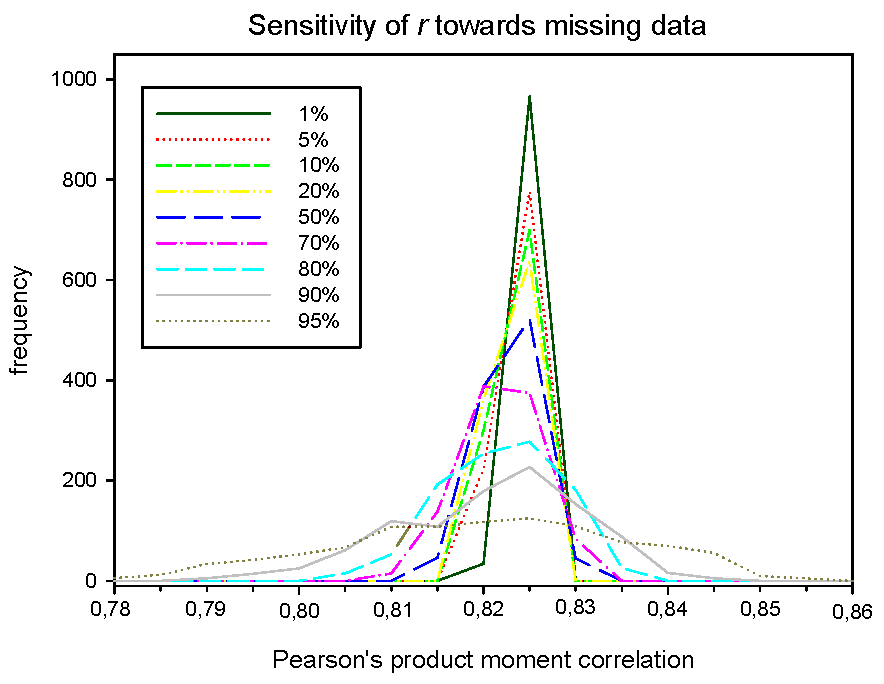
\includegraphics[width=0.75\textwidth]{Graphics/Simulation-MissingValues}
\end{figure}

It is possible to calculate the correlation matrix \arr{R} robustly towards missing values (see fig. \ref{fig:Miss}). However, the resulting matrix will no longer be positive definite and large eigenvalues will be overestimated, while small eigenvalues are underestimated. To be suitable for factor analysis or PCA, \arr{R} must be
\begin{description}
  \item[positive definite]{which means that \(\AbsVec{x}^T \arr{R} \AbsVec{x} > 0\enspace \forall\enspace \AbsVec{x} \) with at least one element \(\neq 0 \). A positive definite matrix has a determinant \(||\arr{R}|| > 0 \). In our case, \(||\arr{R}|| = \num{e-56} \approx 0 \). For a positive definite matrix all leading principal minors (the \skalar{i}-th \textbf{leading principal minor} of an \(n \times n \) matrix is the determinant of the submatrix containing its first \skalar{i} rows and its first \skalar{i} columns) are also positive (\Name{Sylvester}'s criterion). Computational errors may result in small positive or negative values instead of zero for semi-definite matrices.}
  \item[invertible]{No data column \skalar{i} may be a constant, as this would result in \(\arr{R}_{\cdot i} = \arr{R}_{i\cdot} = 0 \). No data column \skalar{i} can be replicated by a linear combination of any of the remaining \(p-1 \) columns, otherwise the \skalar{i}-th row and column of \arr{R} will be linear combinations of other columns or rows, respectively and therefore \(||\arr{R}|| = 0 \).}
\end{description}

\subsubsection{Shrinkage of \arr{S}}\label{text:shrinkage}

The \Name{Ledoit-Wolf}-procedure \parencite{Scha-05,Kwa-11,Led-03} tries to turn a semi-definite matrix into a definite  by ``shrinkage''. In effect, all eigenvalues are moved towards their grand mean, while maintaining the eigenvectors.

\paragraph{Weighted average of \arr{S} with another matrix}
For example, a \(\arr{B}_{p \times p} \) diagonal matrix with \(\arr{B}_{ii} = \arr{S}_{ii} \) the variances in the diagonal (that is, \(\arr{B} = \diag(\arr{S}) \)) is always positive definite, because \(\AbsVec{x}^T \arr{B} \AbsVec{x} = \sum_{j=1}^{p} \AbsVec{x}_j^2 \arr{B}_{jj} > 0 \) if there is at least one element \(\AbsVec{x}_j \neq 0 \). Then the weighted average of \arr{B} and \arr{S} is defined as \(\widehat{\arr{S}} = (1-\omega)\arr{S} + \omega \arr{B} \) with a weight \(0 < \omega < 1 \), and is always positive definite because \(\AbsVec{x}^T \widehat{\arr{S}} \AbsVec{x} = (1-\omega) \AbsVec{x}^T \arr{S} \AbsVec{x} + \omega \AbsVec{x}^T \arr{B} \AbsVec{x} > 0 \). If \(\omega = 0 \), then \(\widehat{\arr{S}} = \arr{S} \), and if \(\omega = 1 \), then \(\widehat{\arr{S}} = \arr{B} \).

\paragraph{Optimal \skalar{\omega}}
The covariances \(s_{ij}, i \neq j \) in \arr{S} are sample estimators of the population covariances \skalar{\sigma_{ij}}. Then \([(1-\omega) s_{ij} - \sigma_{ij}]^2 \) can be viewed as loss, and we would like to find the \(\omega \) that minimises \(\sum_{i=1}^p{\sum_{j=i+1}^{p}{[(1-\omega) s_{ij} - \sigma_{ij}]^2}} \) for all elements of the upper triangle of \arr{S} (of course, the lower triangle would give the same result because of symmetry) \parencite{Kwa-11}. Then
\begin{equation} \label{eqn:omegaW}
  \omega = \frac{\sum_{i=1}^p{\sum_{j=i+1}^{p}{\var(s_{ij})}}}{\sum_{i=1}^p{\sum_{j=i+1}^{p}{[\var(s_{ij}) + \sigma_{ij}^2]}}}
\end{equation}
We note that because the nominator is larger than the denominator and both are positive, the condition \(0 < \omega < 1 \) is met by necessity. To get \(\var(s_{ij}) \) we introduce for each pair of variables \(i,j = 1..p \)  a random variable \(\AbsVec{g}_{ij} \), which is the product of the centered data columns \(\AbsVec{X}_{\cdot{i}} \) and \(\AbsVec{X}_{\cdot{j}} \). Then \(\bar{\AbsVec{g}}_{i,j} = 1/n \sum_{k=1}^{n}{[(\AbsVec{X}_{k,i} - \bar{\AbsVec{x}}_i) (\AbsVec{X}_{k,j} - \bar{\AbsVec{x}}_j)]} \) and \(\var(s_{i,j}) = \frac{n}{(n-1)^3} \sum_{k=1}^n{(\AbsVec{g}_{kij} - \bar{\AbsVec{g}}_{i,j})^2} \) and \(E(s_{i,j}) = \sigma_{i,j} \) and hence \(\sigma_{ij}^2 = s_{i,j}^2 \) \skalar{\omega} can be calculated.

\paragraph{Non-linear shrinkage}
In the simplest case, shrinkage is done linearly by a certain factor \skalar{\omega} as discussed.  Nonlinear shrinkage has been shown to be at least as effective, and most of the time more, than linear \parencite{Led-17}. R package \texttt{nlshrink} provides this method. The method is described for \arr{S}, it is unclear how this would extend to \arr{R}.

\subsubsection{Shrinking a correlation matrix \arr{R}}

Under some simplifying assumptions, the basic idea is the same as with the variance-covariance matrix, but shrinkage is achieved by calculating a weighted average between \arr{R} and the identity matrix \arr{I} \parencite{Scha-05,Kwa-11}. Then equation \ref{eqn:omegaW} becomes
\begin{equation} \label{eqn:omegaR}
  \omega = \frac{\sum_{i=1}^p{\sum_{j=i+1}^{p}{\var(r_{ij})}}}{\sum_{i=1}^p{\sum_{j=i+1}^{p}{[\var(r_{ij}) + \rho_{ij}^2]}}}
\end{equation}
where \(\rho_{ij} \) is the population correlation coefficient of variables \skalar{ij}. \(\var(r_{ij}) = \frac{\var(s_{ij})}{s_{ii} s_{jj}} \) and \(\rho_{ij}^2 = \frac{s_{ij}^2}{s_{ii} s_{jj}} \). The R-package \texttt{corpcor} provides shrinkage for \arr{S} and \arr{R}.

\begin{figure}
   \caption{Effect of shrinkage (using \(\bar{\arr{R}} \)) on a correlation matrix that is not positive semi-definite. With increasing \(\omega \) the correlation coefficients move towards the common mean, the distribution becomes narrow and steep. An \(\omega = 0.5\ldots 0.6 \) is optimal with this matrix, further increases of \(\omega \) have no beneficial effect.}
   \label{fig:shrink1}
   \centering
      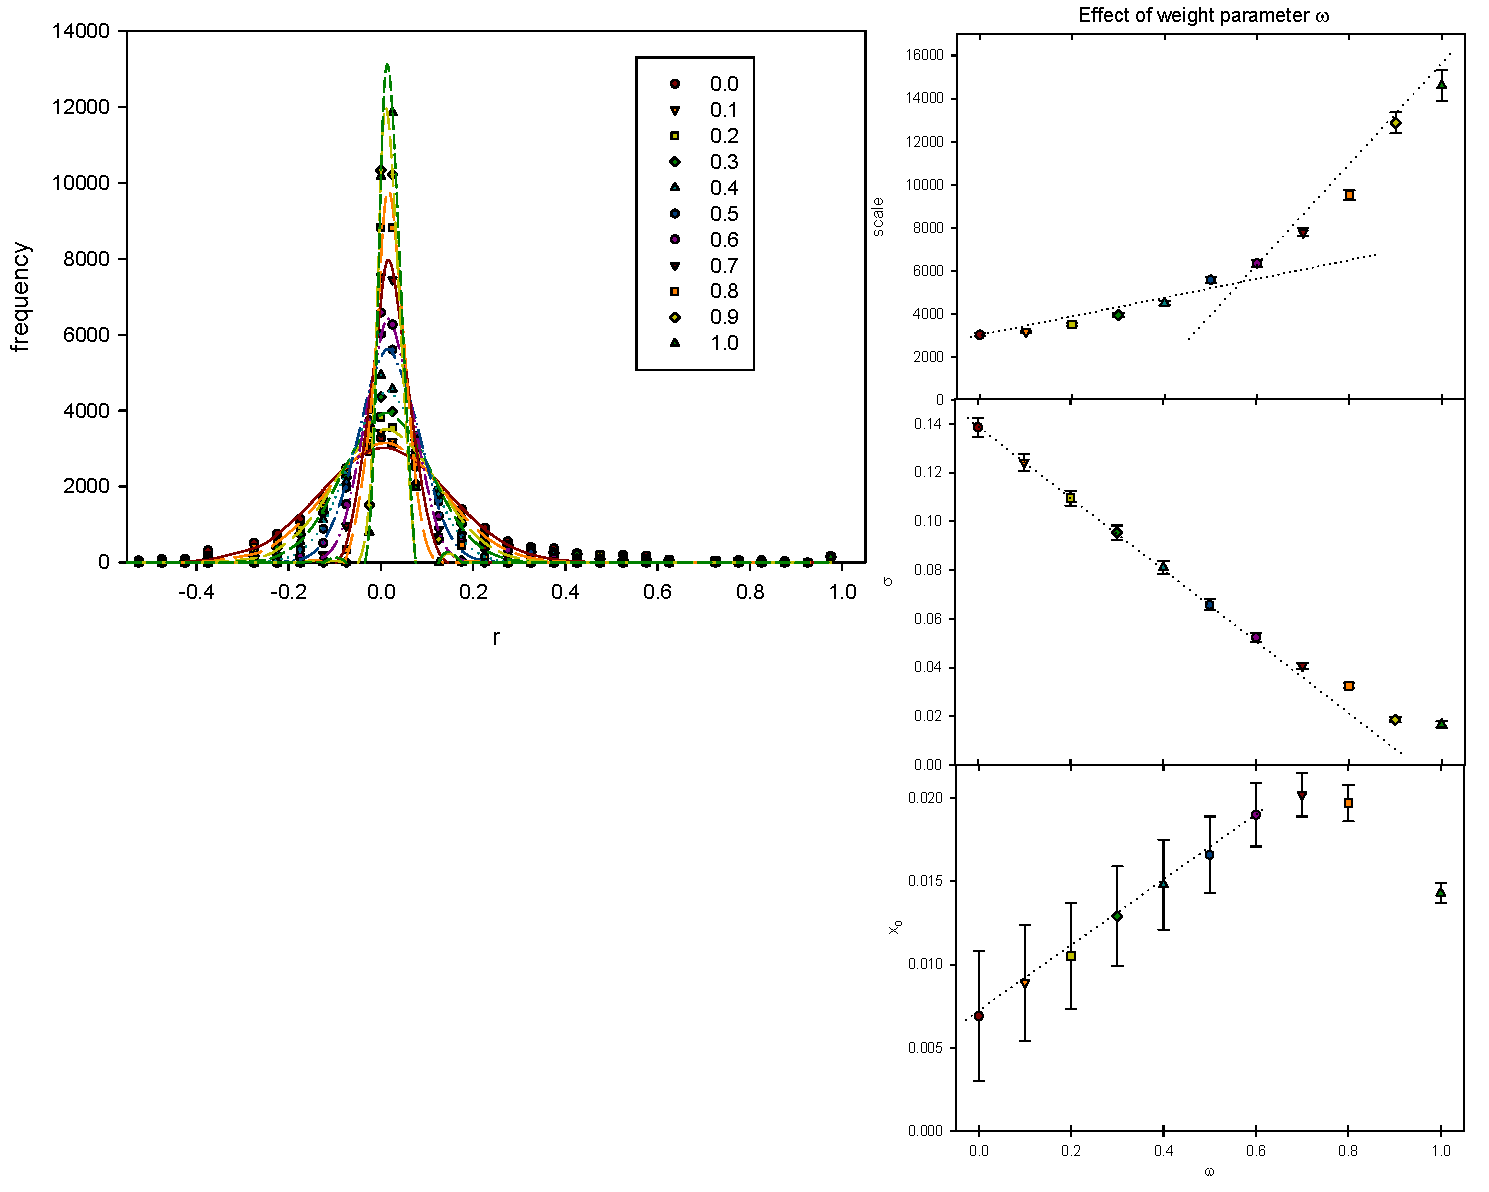
\includegraphics[width=\textwidth]{Graphics/Effect-omega-on-r}
\end{figure}

\begin{figure}
   \caption{Effect of shrinkage (using \(\bar{\arr{R}} \)) of a correlation matrix that is not positive semi-definite. With increasing \(\omega \) the number of positive eigenvalues increases, the maximum cumulative explained variance decreases. An \(\omega = 0.5\ldots 0.6 \) is optimal with this matrix, further increases of \(\omega \) have no beneficial effect. In the scree-plot the lines of different \(\omega \) intersect in a common point, this point is to the right of the number of valid components.}
   \label{fig:shrink2}
   \centering
      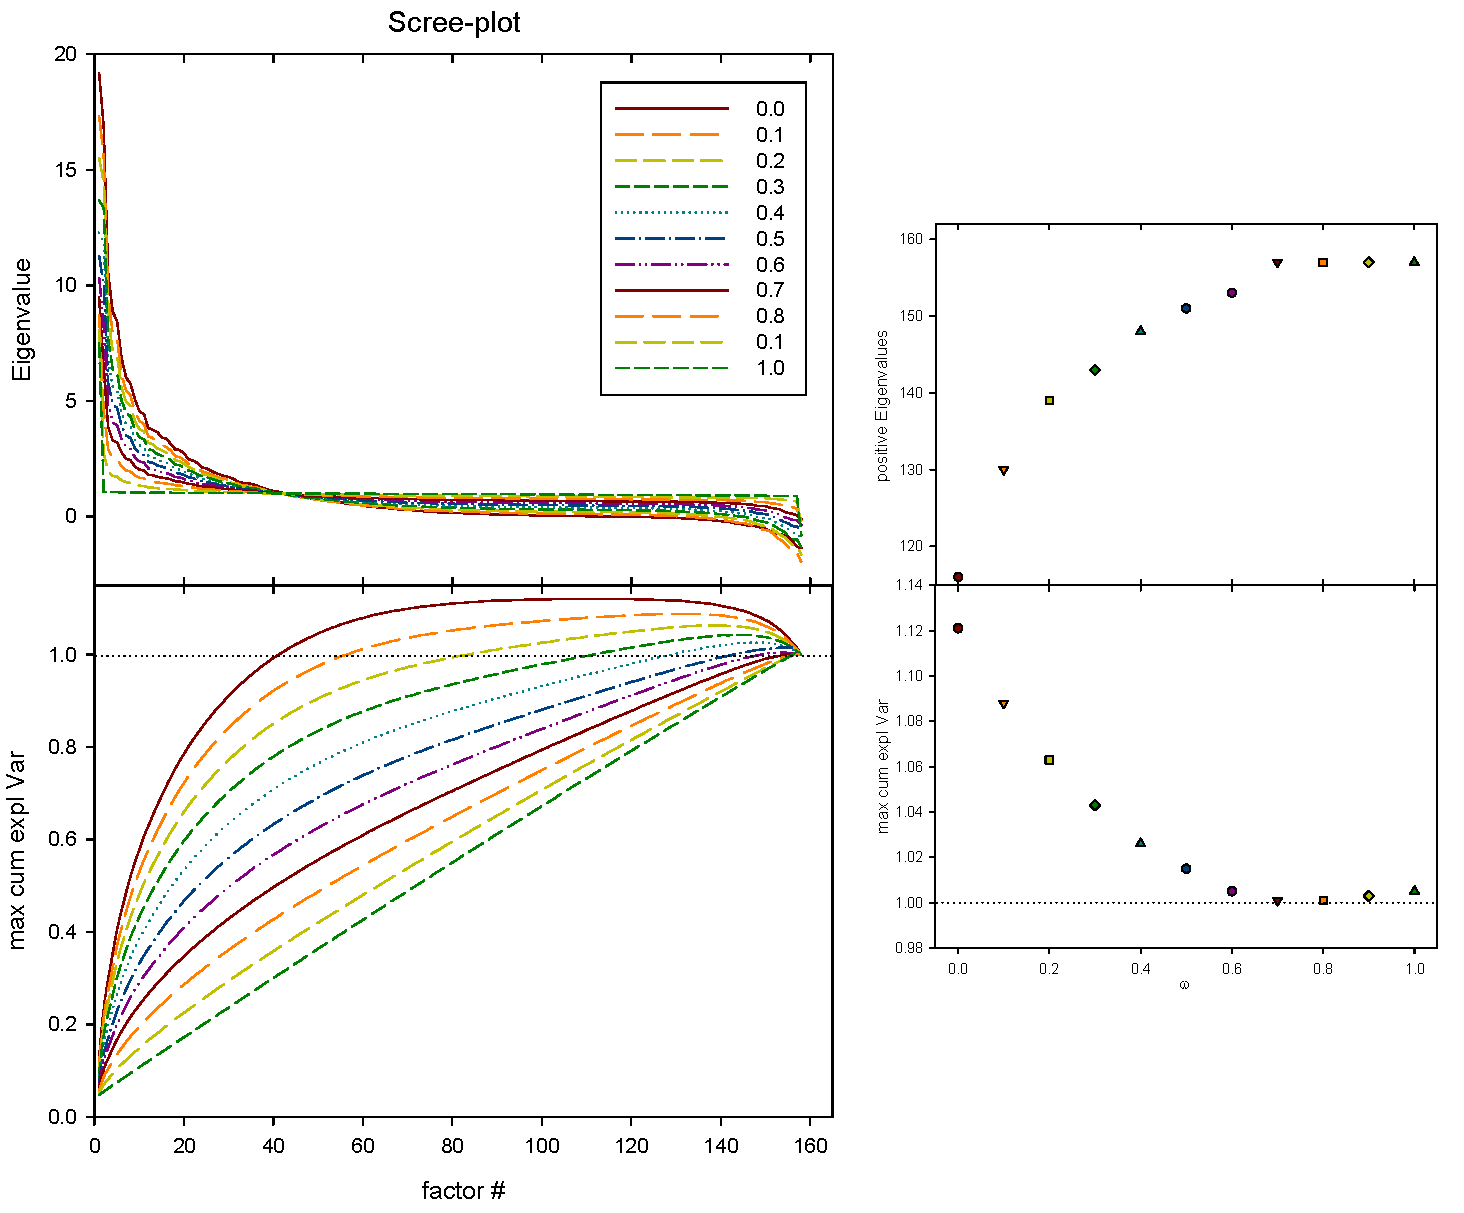
\includegraphics[width=\textwidth]{Graphics/Effect-omega-on-Scree}
\end{figure}

Alternative is to first calculate the average correlation of each variable with all others:
\begin{equation}
   \bar{\skalar{r}}_{i\cdot} = \frac{1}{p-1} \sum_{j=1}^p{\skalar{r}_{ij}} \enspace \forall \enspace j \neq i
\end{equation}
Then the correlation coefficient \(\hat{\skalar{r}}_{ij} = (\bar{\skalar{r}}_{i\cdot} + \bar{\skalar{r}}_{j\cdot}) /2 \) \parencite{Dis-07}. This matrix is positive definite and performs very similar to that described by \parencite{Kwa-11} with optimal \(\omega \) (see fig. \ref{fig:shrink1} and \ref{fig:shrink2}).

\paragraph{Recalculation of \arr{R} and \arr{S} from results of an initial eigenanalysis}

If the correlation matrix \arr{R} is indefinite and returns negative eigenvalues, these can be seen as experimental error (they are usually small). Hence, they are set to zero and a definite correlation matrix \(\widehat{\arr{R}} \) is produced from the corrected eigenvalue matrix \(\diag(\hat{\lambda}) = \hat{\Lambda} \) and the eigenvectors \arr{E} by
\begin{equation}
  \widehat{\arr{R}} = \arr{E} \hat{\Lambda}\ \arr{E}^{-1}
\end{equation}
Then the final eigenanalysis is performed on \(\widehat{\arr{R}} \) \parencite{TL-07}.

It was found, however, that the result of this procedure are \SI{0.5}{\%} correlation coefficients that are outside the range \([-1..+1] \), and many diagonal elements \(\neq +1 \). If this is corrected, negative eigenvalues return, but fewer than with the original correlation matrix. Hence this procedure can be repeated iteratively, until the number of illegal entries in the correlation matrix becomes zero.

\begin{lstlisting}[caption=Correction of non-definite correlation matrices]
  UNIT PerformShrinkage;

  INTERFACE

  USES Math, MathFunc, Vector, Matrix, EigenValues;

  PROCEDURE ErzeugeLambda(CONST Eigenvalues: VectorTyp; VAR Lambda: MatrixTyp);
  { Turn vector of eigenvalues into a diagonal matrix }

  PROCEDURE Average(VAR R: MatrixTyp; omega: double);
  { Shrink the correlation matrix R by calculating the weighted average between R
    and the row means of R for each i and j. omega (0..1) is the relative weight
    of of the average, the relative weight of R is (1-omega) }

  PROCEDURE Shrinkage(VAR R: MatrixTyp; omega: double);
  { Shrink the correlation matrix R by calculating the weighted average between R
    and the identity matrix. omega (0..1) is the relative weight of I, the relative
    weight of R is (1-omega) }

  PROCEDURE NormaliseCorrelations(VAR R: MatrixTyp);
  { make an indefinite correlation matrix positive definite for eigenanalysis,
    by setting all eigenvalues < 0 to zero and re-calculating R = E Lambda E^{-1}. }

  IMPLEMENTATION

  PROCEDURE ErzeugeLambda(CONST Eigenvalues: VectorTyp; VAR Lambda: MatrixTyp);

  VAR
    p, i, j: WORD;

  BEGIN
    p := VectorLength(Eigenvalues);
    CreateIdentityMatrix(Lambda, p);
    FOR j := 1 TO p DO
      SetMatrixElement(Lambda, j, j, GetVectorElement(Eigenvalues, j));
  END;


  PROCEDURE Average(VAR R: MatrixTyp; omega: double);

  VAR
    p, i, j: WORD;
    Averages: VectorTyp;
    Sum, w: double;

  BEGIN
    IF (omega < 0) OR (omega > 1)
      THEN
        BEGIN
          Writeln('Shrinkage: omega not in [0..1]');
          HALT;
        END;
    p := MatrixRows(R);
    CreateVector(Averages, p, 0);                // calculate row-averages OF R
    FOR i := 1 TO p DO
      BEGIN
        Sum := 0;
        FOR j := 1 TO p DO
          IF (i = j)
            THEN  // ignore correlation WITH self
            ELSE  Sum := Sum + GetMatrixElement(R, i, j);
        SetVectorElement(Averages, i, Sum / Pred(p));
      END;
    w := 1 - omega;
    omega := omega / 2;                               // weight FOR each r_i AND r_j
    FOR i := 1 TO p DO                              // calculate NEW elements OF R
      FOR j := Succ(i) TO p DO
        BEGIN
          Sum := (W * GetMatrixElement(R, i, j) + omega *
            GetVectorElement(Averages, i) + omega * GetVectorElement(Averages, j));
          SetMatrixElement(R, i, j, Sum);
          SetMatrixElement(R, j, i, Sum);
        END;
    DestroyVector(Averages);
  END;


  PROCEDURE Shrinkage(VAR R: MatrixTyp; omega: double);

  VAR
    p, i, j: WORD;
    Sum, w: double;

  BEGIN
    IF (omega < 0) OR (omega > 1)
      THEN
        BEGIN
          Writeln('Shrinkage: omega not in [0..1]');
          HALT;
        END;
    w := 1 - omega;
    p := MatrixRows(R);
    FOR i := 1 TO p DO                              // calculate NEW elements OF R
      FOR j := Succ(i) TO p DO
        BEGIN
          Sum := (W * GetMatrixElement(R, i, j)); // non-diagonal elements OF I are 0
          SetMatrixElement(R, i, j, Sum);        // AND can be ignored
          SetMatrixElement(R, j, i, Sum);
        END;
  END;


  PROCEDURE NormaliseCorrelations(VAR R: MatrixTyp);

  VAR
    Eigenvalues: VectorTyp;
    Eigenvectors, Hilfs, Lambda, RecipEV: MatrixTyp;
    i, iter, n, NoNegs, j: WORD;
    Rneu: double;

  BEGIN
    n := MatrixRows(R);
    Writeln('Initial calculation of eigenvalues');
    iter := 1;
    REPEAT
      INC(iter);
      i := Jacobi(R, Eigenvalues, Eigenvectors, j);  // eigenanalysis
      Write(iter: 2, ': ', j: 3, ' iterations, Result = ', i: 1);
      CASE i OF
        0    : Write(' ok             ');
        5    : Write(' no convergence ');
        ELSE   Write(' error          ');
      END;
      NoNegs := 0;
      FOR i := 1 TO n DO
      BEGIN
        IF (GetVectorElement(Eigenvalues, i) < 0)
          THEN
            BEGIN
              SetVectorElement(Eigenvalues, i, 0);
              INC(NoNegs);
            END;
      END;
      Writeln(NoNegs: 3);
      DestroyMatrix(R);
      ErzeugeLambda(Eigenvalues, Lambda);
      CopyMatrix(EigenVectors, RecipEV);
      InverseMatrix(RecipEV);
      MatrixInnerProduct(EigenVectors, Lambda, Hilfs);    // calculate R = E Lambda E^{-1}
      MatrixInnerProduct(Hilfs, RecipEV, R);
      DestroyMatrix(EigenVectors);
      DestroyMatrix(RecipEV);
      DestroyMatrix(Hilfs);
      DestroyMatrix(Lambda);
      DestroyVector(EigenValues);
      FOR i := 1 TO n DO
        BEGIN
          FOR j := 1 TO n DO
            BEGIN
              Rneu := GetMatrixElement(R, i, j);
              IF (Abs(Rneu) > 1.0)
                THEN SetMatrixElement(R, i, j, sign(Rneu));  // max + OR - 1
            END;
          SetMatrixElement(R, i, i, 1.0);                 // diagonal elements 1
        END;
    UNTIL (iter >= 100) OR (NoNegs = 0);
  END;

  END.
\end{lstlisting}

The various methods of shrinkage perform similarly in practice, so numerical simplicity can be the overriding selection criterium \parencite{Dis-07}. The one exception is the recalculation of \arr{R} and \arr{S} from initial eigenanalysis, which raises suspicion against that method.

\subsection{Effect of discrete variables on PCA}

Component analysis was originally developed for interval- and rational scaled variables with multivariate normal distribution. In \parencite{Kol-04} the effects of the use of ordinal and binary scaled, and/or non-normally distributed variables (skew and kurtosis) is investigated. If one assumes that categorial data are generated by quantising underlying cardinal data (with \( < 5 \) categories) the correlation coefficients will be biased towards 0 (their fig. 2). This will affect the principal component weights. Categorization can be viewed as a measurement error with nonlinear properties. Errors can be minimised if all categories have similar numbers of observation. \acs{PCA} is quite robust toward different distances between the categories of a variable.  On average, a discrete variable contains 2/3 of the information of the underlying cardinal variable.

Sometimes dummy variables corresponding to individual categories are used. \Foreign{E.g.}, an ordinal value for affluence may be mode of transport (walk, bicycle, motorcycle, car). One could replace this with four independent, binary variables (has car, has motorcycle...). However, the natural order of the variable, and hence information, would be lost. Also, the effect of quantisation is aggravated. Most weight is attached to the category with the highest number of observations. Also, \acs{PCA} becomes numerically less stable.

It is incorrect to use \Name{Pearson}'s correlation coefficient for nominal or ordinal data. The correlation coefficient between two variables is influenced by both their substantive similarity and by their statistical distributions. If the distributions are dissimilar, then \acs{FA} or \acs{PCA} may give a spurious multidimensional results. Polychoric correlations have been successfully tried with \Name{Likert}-scale data \parencite{Bas-12}.

\subsection{Number of components}

\acs{PCA} is used to reduce the dimensionality of the data set, this makes interpretation easier and removes random noise. It may also make further analysis (multiple regression, clustering) more stable by removing co-linearity. However, it also leads to a loss of information. The question therefore is how many components are significant enough to be included in the following analysis. In general, too many components cause fewer problems than too few \parencite{Bas-12}.

\subsubsection{Scree-plot}\label{text:scree}

\begin{figure}
   \caption{Example for a scree-plot, from an investigation on validity of exam questions. The two leftmost components form the mountain and are used for analysis, the remaining components are discarded as rubble. The acceleration is the second derivative of the scree-plot and can sometimes help to identify the ``knee''. Here, it would suggest that third eigenvalue may also be significant.}
   \label{fig:Scree}
   \centering
      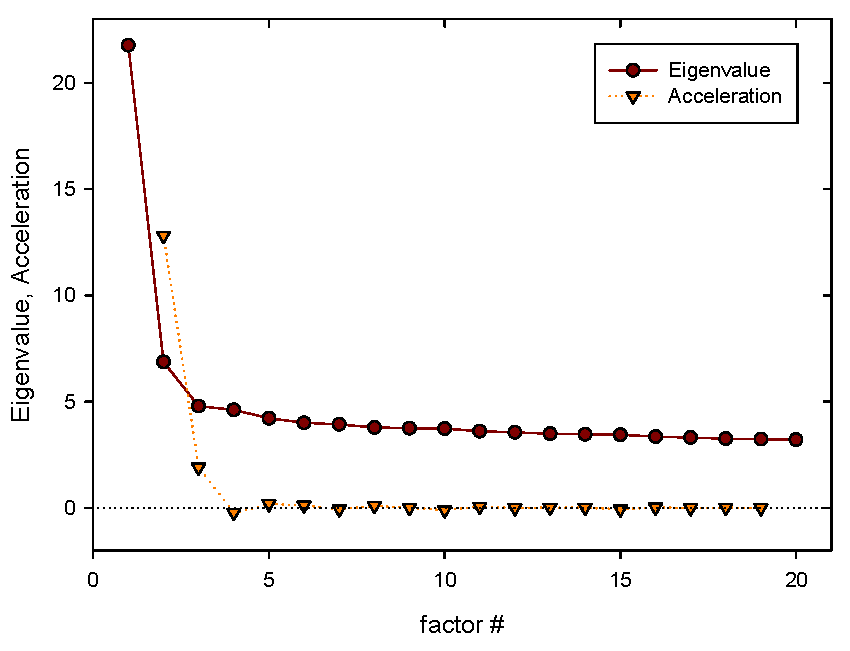
\includegraphics[width=0.75\textwidth]{Graphics/Acceleration}
\end{figure}

In a plot of eigenvalue vs factor or component number (see fig. \ref{fig:Scree}) \parencite{Cat-66} one sees initially a steep exponential decline (``cliff'') followed by a shallow area with linear decline (``rubble'' or ``scree''). The cliff (data left of the ``knee'') represents the significant components. However, distinguishing cliff and scree can be difficult and subjective. The \textbf{acceleration factor} is calculated as the second derivative of the scree-curve by finite differences, \(f''(j) \approx (f(j+1) - 2f(j) + f(j-1)) \), it should have a maximum at the knee. This is usually not discernible, but for non-significant components this value oscillates around zero.

\subsubsection{\Name{Kaiser}-criterion}

All components with an eigenvalue \(> \bar{\lambda} \) are considered significant. This average is \num{1.0} when a \skalar{z}-standardised data matrix is used (or when the eigenanalysis is performed on \arr{R} rather than \arr{S}), so the variance of each variable is \num{1.0}. The eigenvalue is the sum of the squared loadings of a component with all variables and corresponds to the variance explained by this component. However, in an analysis with many variables the \Name{Kaiser}-criterion overestimates the number of significant components, as some eigenvalues will be \(> 1 \) by chance (variables uncorrelated in the population have small correlation in the sample, leading to significant eigenvalues).

\subsubsection{Variance explained}

The retained components are supposed to retain the significant information of the data, but not the noise. One can simply set a minimal value for explained variance, say, \SI{5}{\%} or \SI{10}{\%}. Components that account for less are discarded. Alternatively, enough components are retained so that the cumulative explained variance is \num{70}--\SI{80}{\%}.

\subsubsection{Parallel analysis}

\acs{PCA} is performed both with the empirical data set and with (at least 100) data sets of random numbers (if data are normally distributed) or a permuted data set (if data have a non-normal distribution). The number of cases and variables in the random set should be identical  to the empirical. Only those eigenvalues in the empirical data are considered significant that are larger than those from the random data. Standard statistical packages do not include this computationally expensive method, so it is under-used.

\subsubsection{\Name{Bartlett}'s test for sphericity}

It is possible to use \Name{Bartlett}'s sphericity test to calculate the significance of the difference between eigenvalues. Say, we have a test with \(n = 100 \) persons and \(p = 3 \) variables. The eigenvalues are 8, 4, 2 \parencite{Hop-75}. Then according to eqn. \ref{eqn:Bart} \(r = 0.8571, r^3 = 0.6295, \chi^2 = 44.66 \) and \(f = 5 \), therefore \(P_0 < \SI{0.1}{\%} \). Next, we eliminate the first eigenvalue and calculate the test values for the remaining eigenvalues:
\begin{align}\label{eqn:BartNo}
   r      &= \frac{(4 \times 2)^{1/2}}{1/2 \times (4 + 2)} = \frac{\sqrt{8}}{3} \\
   r^2    &= \frac{8}{9} \notag \\
   \chi^2 &= -(100 - 3 - 1/2) (-0.11779) = 11.37 \notag \\
   f      &= \frac{(3 - 1 + 2) (3 - 1 -1)}{2} = 2 \notag
\end{align}
We then take the difference between both \(\chi^2 \)-values (44.66 - 11.37 = 33.29) and degrees of freedom (5 - 2 = 3) and use the result to test for the significance of the difference between the first and second eigenvalue (\( P_0 < \SI{0.1}{\%} \)). This process is continued until that difference becomes non-significant or until only one eigenvalue is left.

From this procedure we learn how many data are required to \emph{describe} the data, not necessarily how many can be used to \emph{describe} them. For singular correlation matrices \(\chi^2 \) will remain significant for all \skalar{p} components.

\subsubsection{Very simple structure (VSS)}

This method compares the original correlation matrix with that reproduced from the retained eigenvalues and -vectors \parencite{Rev-79}. As the number of retained components increases, VSS index increases sharply to a maximum, then decreases slowly. Procedure:
\begin{enumerate}
  \item{Extract components by the method of your choice, and make an initial estimate of the number of relevant components \skalar{q}}
  \item{Rotate the components by the method of your choice, resulting in a rotated component matrix \(\arr{B}_{p \times q} \)}
  \item{Calculate VSS:
    \begin{enumerate}
      \item{For a VSS of complexity \skalar{v}, replace the smallest \(q-v \) elements of \arr{B} by zero, resulting in a degraded component matrix \(\arr{B}_{p \times q}' \)}
      \item{Calculate the degraded correlation matrix \(\arr{R}' = \arr{B}' \Lambda \arr{B}'^{-1} \)}
      \item{calculate the mean square residual \skalar{M} of both \arr{R} and \arr{R}' and \(\mathrm{VSS}_{v,p} = 1 - \frac{M_{\arr{R}'}}{M_\arr{R}} \)}
    \end{enumerate} }
  \item{Repeat this for all \skalar{q} from 1 to the rank of the matrix and plot the results against \skalar{q}}
\end{enumerate}

\subsubsection{\Name{Velicer}'s minimum average partial (MAP) criterium}
\parencite{Vel-76}. The test has been revised with the partial correlations raised to the 4th power
(rather than squared). Source code is available under \href{https://people.ok.ubc.ca/brioconn/nfactors/nfactors.html}{https://people.ok.ubc.ca/brioconn/ nfactors/nfactors.html} and in the R-package \texttt{paramap}.

\subsubsection{Extrapolation}

One can draw a line between the \skalar{p}-th eigenvalue and the \skalar{i+1}-th. Then one can estimate the \skalar{i}-th eigenvalue by extrapolation. Measured eigenvalues are considered relevant if they are significant larger than the estimated one. This method is used by the R-module \texttt{nFactors}.

\subsubsection{Newer methods}

\Name{Gavish \& Donoho} \parencite{Gav-14} have shown that for a data matrix which is large compared to its rank, the optimal number of singular values to retain is \(\omega\tilde{\sigma} \), where \skalar{\tilde{\sigma}} is the median of the singular values. For \skalar{n \times p} matrices, \skalar{\omega} depends on \(\beta = p / n \) as \(\omega(\beta) \approx 0.56\beta^3 - 0.95\beta^2 + 1.82\beta + 1.43 \).

\Name{Minka} \parencite{Min-00} uses \Name{Bayes}ian statistics to derive a probability function that reaches its highest value at the optimal number of components
\begin{eqnarray}
   \nonumber
   \hat{v}      =& \frac{\sum_{j=q+1}^p{\lambda_j}}{p-q} \\
   \nonumber
   m            =& pq - \frac{q(q+1)}{2} \\
   P(\arr{X}|q) =& \left(\prod_{j=1}^q{\lambda_i}\right)^{-n/2} \hat{v}^{-n(q-q)/2} n^{-(m+q)/2}
\end{eqnarray}
where \skalar{\hat{v}} is the average of the left-out eigenvalues, that is, the maximum-likelihood noise variance.

\subsubsection{Importance of minor components}

Components that explain only a small percentage of the variance of the population as a whole may explain a large part of the variance of a small number of persons. For example, in a psychiatric test the answer to the question ``Did somebody ever try to murder you?'' will be ``no'' for the vast majority of subjects. A component loading on this question therefore might be dropped as noise. However, for the few people who answer ``yes'', the discriminatory value of that question might be quite high. It can therefore be useful to look for individuals that score high on such minor components.


     % -*- TeX:UK -*-
\section{Rotation of factors or components}

\begin{figure}
   \caption{Eigenvectors plotted into the coordinate system of the components obtained. All eigenvectors of \acs{PCA} have unit length and point from the centre to the circumference of a unit circle (sphere or spheroid in higher dimensional cases). Rotation of the coordinate system (\emph{blue arrow}) achieves a structure that is simpler to interpret. The angles between the original and the new coordinate axis are called \(\theta_{xy}, \theta_{xx}, \theta_{yx}, \theta_{yy} \), respectively. They are measured in mathematically positive direction (counterclockwise).}
   \label{fig:RotGeo}
   \centering
      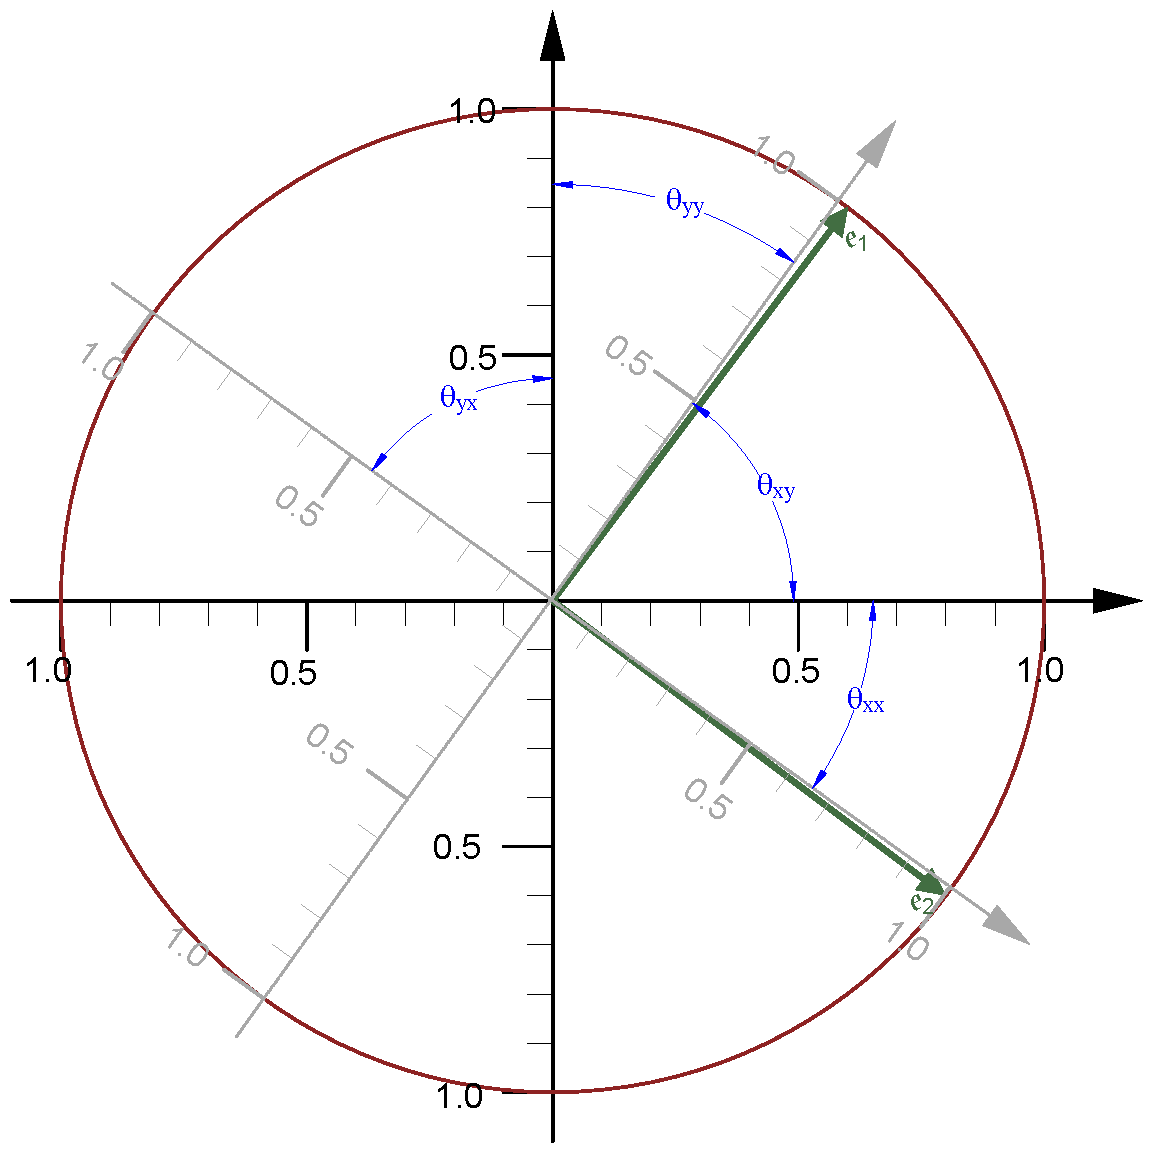
\includegraphics[width=0.75\textwidth]{Graphics/Rotation}
\end{figure}

To make the result of a factor analysis (or \acs{PCA} if it is used as proxy for \acs{FA}) more interpretable the found factors are rotated to achieve a simple structure \parencite{Thur-47}. A simple structure should fulfill the following criteria (for more than four factors extracted):
\begin{itemize}
  \item{each row (variable) contains at least one near zero}
  \item{each column (factor) should have several near zeros}
  \item{for any pair of factors, there are
     \begin{itemize}
       \item{some variables with near zero loadings on one factor and large loadings on the other}
       \item{a sizable number of variables that have near zero loadings on both}
       \item{a small number of variables that have large loadings on both}
     \end{itemize} }
\end{itemize}
Geometrically, the loadings in each row of the loading matrix constitute the coordinates of a point in loading space. If there are clusters of points, we try to put our axes near these clusters, so that each group of variables becomes associated with a factor. If all points are close to an axis, then they would load highly on the corresponding factor, and only little on all others. The complexity of a variable is the number of factors that this variable has moderate or high loadings on. The simple structure then has a complexity of 1.

In other words, the variance of factor loadings per factor is maximised. Note that since rotation is performed only on the factors retained, the result of rotation will change if more or fewer factors are retained. There are two classes of rotation, each with several methods \parencite{Kie-98,Abd-03,Cla-88}:
\begin{description}
  \item[orthogonal]{only right angles between axes are allowed, factors are uncorrelated. The \emph{orthomax function} maximised is \(Q_\mathrm{max}  = \sum_{j,k = 1}^{p, q}{\AbsVec{l}_{jk}^4} - \gamma/p \sum_{k=1}^q{(\sum_{j=1}^p{\AbsVec{l}_{jk}^2})^2} \).
     \begin{description}
        \item[Varimax]{was introduced by \Name{Kaiser} \parencite{Kai-58,Kai-59} and expressed in matrix terms by others \parencite{She-66,Nev-86}. The axes are rotated until all loadings become either large or small, thereby number of variables with high loadings on several factors is minimised. The orthomax function is used with \(\gamma = 1 \). }
        \item[Quartimax]{The number of factors required to explain a variable is minimised, this makes interpretation of the variables easier. The orthomax function is used with \(\gamma = 0 \).}
        \item[Equamax]{is a mixture of Varimax and Quartimax.}
    \end{description} }
  \item[oblique]{angle between axes may be different from \ang{90}, there is correlation between rotated factors. However, this correlation is small, as highly correlated factors would be better interpreted as one factor. Oblique rotations produce two matrices as solution, called pattern and structure matrix, respectively. The most important oblique methods are:
    \begin{description}
        \item[Promax]{is fast and therefore the most frequently used oblique rotation, especially with large data sets. A target matrix is calculated from a varimax rotation whose loadings are raised to a power \(\num{2} < \kappa < \num{4} \), maintaining the sign. This reduces the loadings, but increases the ratio of loadings. Often, an average between the varimax and promax solutions is calculated (procrustean rotation).}
        \item[Oblimin]{produces results that look very much like varimax, except that they are oblique. The degree of obliqueness allowed is controlled by a parameter \textdelta, negative values decrease factor correlation, positive increase it. \(\delta = -4 \) produces uncorrelated factors, default in SPSS is \num{0}, maximum should be \num{0.8} or so. The method minimises the cross-product between loadings, the \emph{oblimin criterium} minimised is \(Q_\mathrm{min} = \sum_{r \neq s}{\left(\sum_{j=1}^p{\AbsVec{l}_{jr}^2\AbsVec{l}_{js}^2} - \gamma/p \sum_{j=1}^p{\AbsVec{l}_{jr}^2} \sum_{j=1}^p{\AbsVec{l}_{js}^2}\right)} \). The special cases of \(\gamma = 0 \) and \(\gamma = 1 \) are called \textbf{quartimin} and \textbf{covarimin}, respectively.}
    \end{description} }
\end{description}
An orthogonal rotation matrix \(\Theta \) is defined, where the rows represent the original and the columns the new  axes \parencite{Abd-03}. Each element of the matrix is the cosine of the angle between the old and new axis, measured in mathematically positive direction (counterclockwise, see fig. \ref{fig:RotGeo})). For the 2D-case:
\begin{gather}
   \Theta = \begin{pmatrix}
                \cos(\theta_{xx}) & \cos(\theta_{xy}) \\
                \cos(\theta_{yx}) & \cos(\theta_{yy}) \\
            \end{pmatrix}
          = \begin{pmatrix}
                \cos(\theta_{xx}) & -\sin(\theta_{xx}) \\
                \sin(\theta_{xx}) &  \cos(\theta_{xx}) \\
            \end{pmatrix}
\end{gather}
This matrix is orthonormal (\( \Theta^T\Theta = \arr{I} \)). The purpose of rotation is to maximise \(Q_\mathrm{max} \) (or minimise \(Q_\mathrm{min} \))

Some authors claim that it is better to perform an oblique rotation first, and a orthogonal only if the resulting angles between factors are not very different from \ang{90} \parencite{Cos-05}. This way, one doesn't enforce a structure which the data don't have. On the other hand, if two factors are correlated (angle significantly different from \ang{90}), then what causes the correlation? In addition, oblique rotation induces additional variability that will make replication of the results in future studies less likely (less factor invariance). The arbitrary setting of \textkappa\ and \textdelta\ by the researcher adds to this problem. The better fit of oblique rotations may be a result of over-fitting. When \acs{PCA} rather than \acs{FA} is used to extract factors, the resulting factors (actually: components) are by definition uncorrelated and oblique rotation will produce similar results to orthogonal.

If there is a strong factor structure in the data, the results from various rotation methods should look similar, if they don't you have a problem anyway. Therefore, the simplest method (varimax) may be used as default.

\begin{figure}
 \caption{Redistribution of explained variance between factors due to rotation. The total explained variance doesn't change, but the relative importance of the components does. }
 \label{fig:trace}
 \centering
 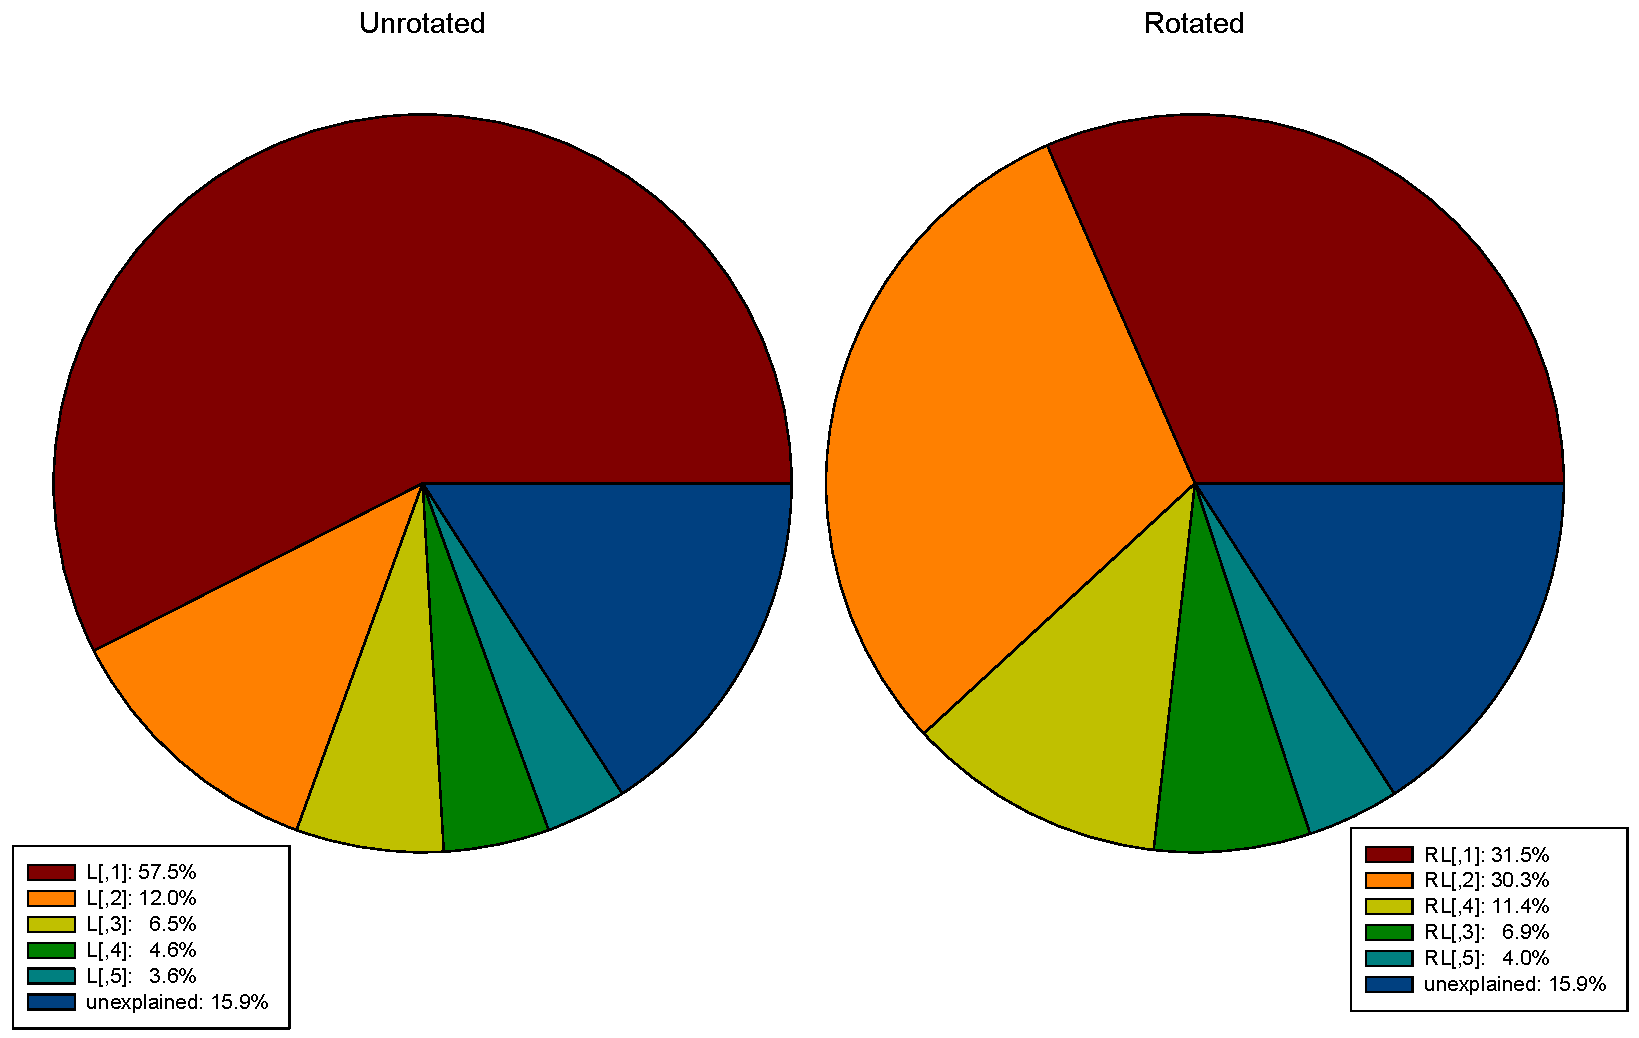
\includegraphics[width=\textwidth]{Graphics/Effect-rotation}
\end{figure}

After rotation, the new loading matrix \arr{L}' reproduce the covariance matrix just like \arr{L}:
\begin{equation}
  \arr{S} = \arr{L}'\arr{L}'^T + \Psi = \arr{L}\theta\theta^T\arr{L}^T  + \Psi = \arr{L}\arr{L}^T  + \Psi
\end{equation}
with \(\Psi_p \) the specific variance. However, the relative importance of factors changes, and is no longer given by the original eigenvalues (see fig. \ref{fig:trace}). A new variance-accounted-for statistics, the \textbf{trace}, is used. After orthogonal rotation, the trace are the column sums of squared factor loadings, and the communalities the row sums (just as in the unrotated case). For oblique rotations, the pattern coefficients are multiplied with the corresponding structure coefficient, the results are summed column-wise for the trace and row-wise for the communalities.

\subsection{Mathematical procedure for orthogonal rotation}

\subsubsection{Gradient projection algorithm (GPA)}\label{text:GPA}

If \arr{L} is the loading matrix, and \( Q_\mathrm{min}(\arr{L}) \) a rotation criterium, then this criterium is to be minimised over all possible rotations, defined in the rotation matrix \( \Theta \). The rotation then becomes \parencite{Jen-01} \( \arr{L}' = \arr{L} \Theta \) and the function to be minimised over all \( \Theta \) is \( f(\Theta) = Q_\mathrm{max}(\arr{L}\Theta) \). For algorithms like varimax, which originally required maximising a quality function, we simply take the negative. The basic algorithm then becomes:
\begin{enumerate}
  \item{Choose an \( \alpha \geq 0 \) and a rotation matrix \( \Theta \) (can be the identity matrix or a random orthogonal matrix) }
  \item{Compute \( \arr{G} = df/d\Theta \), with \( df/d\Theta \) the matrix of partial derivatives }
  \item{Move \( \alpha \) units down the gradient by computing a singular value decomposition \( \arr{U}\Delta\arr{V}^T \) of \( \arr{G} + \alpha\Theta \) }
  \item{Replace \( \Theta \) by \( \arr{UV}^T \)}
  \item{either go to 2) or stop }
\end{enumerate}
This algorithm will converge stationary if \( \alpha \) is sufficiently large. The differential \( \arr{G} = df/d\Theta = \arr{L}^T \frac{dQ}{d\arr{L}'} \) for the quartimax function \(Q(\arr{L}') = 1/4 \sum{\sum{\AbsVec{l}_{jk}^4}} \) becomes \( \frac{dQ}{d\arr{L}'} = \arr{L}'^3 \), which is the element-wise cube of \arr{L}'. For quartimax and varimax rotation, \( \alpha = 0 \) is sufficient to ensure convergence in a few steps. A fixed point of \( \Theta \), that is a \( \Theta \) that doesn't change when the algorithm is applied to it, is also a stationary point of \( f(\Theta) \). It can be shown that with sufficiently large \( \alpha \) the algorithm converges monotonically toward such a fixed point, independently of the starting value of \( \Theta \). As a stationary point is approached, the measure \skalar{v} approaches zero: \(v = ||\mathrm{skm} \Theta^T \arr{G}|| + ||(\arr{I} - \Theta \Theta^T) \arr{G}|| \), where the skew-symmetric part of a square matrix is skm(\arr{M}) = \( 1/2 \arr{M}-(\arr{M})^T \). In practice, one can stop the iteration when \( v \leq \num{e-6} \).

\( \alpha \) needs to be large enough to guarantee monotonicity, but too large an \(\alpha \) will make the algorithm run slower. Operationally, one can run the algorithm with a chosen \( \alpha \) (say, 0) and see if \skalar{v} monotonically declines. If not, \( \alpha \) needs to be increased by some \( \Delta\alpha \) until it does. \parencite{Jen-04,Ber-05} provides more general optimisation criteria, component loss functions that use the second, rather than the fourth, power functions, for example an entropy function \( O(\arr{L}') = -\sum{\sum{\AbsVec{l}^2_{j,k} \log{\AbsVec{l}^2_{j,k}}}} \) that results in simpler \arr{L}' than either quartimax or varimax, small changes in the loading matrix at start produce less big changes in final outcome. Code examples may be found at \parencite{Ber-05a}. An interesting case of rotation are the tandem criteria \parencite{Com-67}: A loading matrix is first rotated by tandem 1 to determine the number of relevant factors, the reduced loading matrix is then rotated by the tandem 2 algorithm.

\begin{sidewaystable}
  \caption{Quality criteria and their differentials, all given for minimisation \parencite{Ber-05}. \( \langle\arr{X,Y}\rangle = \trace(\arr{X}^T \arr{Y}) \) represents the \Name{Frobenius}-scalar product of matrices \( \arr{X}_{n\times p}, \arr{Y}_{n\times p} \), \( \langle\arr{X}\rangle = \langle\arr{X^T,X}\rangle = \sqrt{\sum_{i=1}^m{\sum_{j=1}^n{a_{i,j}^2}}} \) the \Name{Frobenius}-norm of the matrix \( \arr{X} \), \( \arr{X}\odot\arr{Y} \) the element-wise (\Name{Hadamard-Schur}) product and \( \arr{X}^2 = \arr{X}\odot\arr{X} \) the element-wise square of a matrix. \arr{I} is the identity matrix, \arr{N} a (compatible) square matrix with \num{0} in the diagonal, \num{1} everywhere else, and \( \arr{M}_{p\times p} \) a matrix with \( \AbsVec{m}_{ij} = 1/p \). \( \AbsVec{U}_p, \AbsVec{V}_q \) are column vectors of \num{1}.  }
  \label{tab:rot}
  \centering
    \small{\begin{tabular}{lll}
      \toprule
      Criterium                & \( Q_\mathrm{min}(\arr{L}') \)                                                                  & \( \arr{G} = df/d\Theta \)                                                             \\
      \midrule
      quartimax                & \( -1/4 \sum_i{\sum_j{\AbsVec{l}_{ij}}} = -\langle\arr{L}'^2, \arr{L}'^2\rangle/4 \)            & \( -\arr{L}'^3 \)                                                                      \\
      oblimin                  & \( \langle\arr{L}'^2,(\arr{I}-\gamma\arr{M})\arr{L}'^2\arr{N}\rangle / 4 \)                     & \( \arr{L}' \odot [(\arr{I} - \gamma \arr{M})\arr{L}'^2 \arr{N}] \)                    \\
      \Name{Crawford-Ferguson} & \( (1 - \kappa)\langle\arr{L}'^2, \arr{L}'^2 \arr{N} \rangle/4 + \kappa \langle\arr{L}'^2, \arr{N}\arr{L}'^2\rangle/4 \)  & \( (1 - \kappa)\arr{L}' \odot \arr{L}'^2\arr{N} + \kappa\arr{L}' \odot\arr{N}\arr{L}'^2 \) \\
      quartimax                & \grqq, \( \kappa = 0 \)                                                                         & \grqq, \( \kappa = 0 \)                                                                \\
      varimax                  & \grqq, \( \kappa = 1/p \)                                                                       & \grqq, \( \kappa = 1/p \)                                                              \\
      equamax                  & \grqq, \( \kappa = q/2p \)                                                                      & \grqq, \( \kappa = q/2p \)                                                             \\
      parsimax                 & \grqq, \( \kappa = \frac{q-1}{p+q-2} \)                                                         & \grqq, \( \kappa = \frac{q-1}{p+q-2} \)                                                \\
      factor parsimony         & \grqq, \( \kappa = 1 \)                                                                         & \grqq, \( \kappa = 1 \)                                                                \\
      \Name{Jennrich} minimum entropy & \( -\langle\arr{L}'^2, \log\arr{L}'^2\rangle/2 \)                                        & \( -\arr{L}' \odot \log(\arr{L}'^2) - \arr{L}' \)                                      \\
      Oblimax                  & \( -\log\langle\arr{L}'^2\rangle^2 + 2 \log\langle\arr{L}'\rangle^2 \)                          & \( -\frac{4\arr{L}'^3}{\langle\arr{L}'^2\rangle^2} + \frac{4 \arr{L}'}{\langle\arr{L}'\rangle^2} \) \\
      tandem criteria I        & \( -\langle\arr{L}'^2, (\arr{L'}\arr{L}^T)^2\arr{L}'^2\rangle \)                                & \( -4\arr{L}' \odot [(\arr{L}'\arr{L}'^T)^2\arr{L}'^2] \)                              \\
      tandem criteria II       & \( \langle\arr{L}'^2, [\arr{U}\arr{U}^T - (\arr{L}'\arr{L}'^T)^2]\arr{L}'^2\rangle \)           & \( 4\arr{L}' \odot {[\arr{U}\arr{U}^T - ((\arr{L}'\arr{L}'^T)^2)]\arr{L}'^2} - 4{[\arr{L}'\arr{L}'^T] [\arr{L}'^2(\arr{L}'^2)^T]} \arr{L}' \) \\
      \bottomrule
    \end{tabular}}
\end{sidewaystable}

\subsubsection{Penalised varimax}

Interpretation of rotated factors may be complicated by the different communalities of each factor. It is possible to constrain rotation so that communalities are the same for all factors \parencite{Tre}. The varimax rotation does a fairly good job in this respect, which may be one of the reasons for its popularity. It maximises \( Q_\mathrm{max}  = \sum_{j,k = 1}^{p, q}{\AbsVec{l}_{jk}^4} - 1/p \sum_{k=1}^q{\left(\sum_{j=1}^p{\AbsVec{l}_{jk}^2}\right)^2} \). The rotation can be defined in matrix terms
\begin{align}
  \nonumber
  \arr{M}(\Theta) &= \arr{N}^T \arr{O} \arr{N} \\
  \nonumber
  \arr{N} &= \arr{L}' \odot \arr{L}'\\
  \arr{O} &= \arr{I} - \frac{\arr{I}\arr{I}^T}{p}
\end{align}
where \(\odot \) represents the \Name{Hadamard-Schur} (elementwise) product of two matrices. \( \arr{M}/(p-1) \) is the covariance matrix of the squared \arr{L}'. Hence we have to maximise \( \sigma(\Theta) = \mathrm{trace}(\arr{M}(\Theta)) \).
In an orthogonal rotation, the sum of squared loadings is not changed, \( \mathrm{trace}(\arr{L}^T \arr{L}) = \mathrm{trace}(\arr{L}'^T) \arr{L}' =\) const. The requirement that all factors should have equal sums of squares means that \( \arr{L}'^T_{\cdot 1} \arr{L}'_{\cdot 1} = \ldots = \arr{L}'^T_{\cdot q} \arr{L}'_{\cdot q} \). In order to achieve this, the varimax function must be modified with an additional constraint \( PV(\Theta) = \mathrm{trace}(\arr{N})^T \arr{O} \arr{N} - \mu \arr{I}^T \arr{N} \arr{N}^T \arr{I} \) with \skalar{\mu} a  positive number that controls the importance of the penalty term, adjusting the result from pure varimax for \skalar{\mu} = 0  to equal sum of squares for large \skalar{\mu}. The gradient of this function is \( 4 \arr{L}^T {\arr{L}' \odot [(\arr{O} - \mu \arr{I} \arr{I}^T) \arr{N}]} \).

\subsection{Pascal code for rotation}

Rotation of loading matrices is performed by gradient projection according to \parencite{Ber-05}, using  R and SAS example code deposited on \parencite{Ber-05a}. For the time being, only orthogonal rotation is implemented. The rotation methods available are listed in an enumeration type. These can be used by the calling program to specify the desired method:

\begin{lstlisting}[caption=Interface of unit Rotation]
  UNIT Rotation;

  { Rotation of loading matrices by gradient projection according to
    C.A. Bernaards & R.I. Jennrich: Gradient Projection Algorithms and Software
    for Arbitrary Rotation Criteria in Factor Analysis,
    Educ. Psychol. Meas. 65:5 (2005) 676-696, doi:10.1177/0013164404272507.
    Some code in R and SAS is deposited on http://www.stat.ucla.edu/research/gpa/ }

  INTERFACE

  USES MathFunc, Vector, Matrix, SingularValue;

  CONST
    Convergence = -5; // log OF convergence criterium considered success

  TYPE
    RotType = (Varimax, Quartimax, Equamax, Parsimax, Parsimony, Quartimin,
      Biquartimin, Covarimin, Entropy, Tandem1, Tandem2);

  PROCEDURE GradProjAlgOrth(VAR Loading, Rotation: MatrixTyp; RotAlg: RotType);
  { Gradient Projection Algorithm for orthogonal rotation. Rotation algorithm used
    is selected by RotAlg.  }

  PROCEDURE CalculateSAL(CONST Loading: MatrixTyp; VAR SAL: VectorTyp);
  { Sorted absolute loadings (SAL) of a loading matrix. }


  IMPLEMENTATION
\end{lstlisting}

\subsubsection{Rotation methods}

The calculation of the gradient matrix and of the quality measure in each rotation are performed in procedures that depend on the rotation method used.

\paragraph{Varimax}

The varimax method \parencite{Kai-58} is one of the oldest, most used and generally successful rotation methods. As alternative to below procedure the \Name{Crawford-Ferguson}-routine with \(\kappa = 1/p \) may also be used. Varimax is used for orthogonal rotation.

\begin{lstlisting}[caption=Varimax]
  PROCEDURE FVarimax(CONST ActLoading: MatrixTyp; VAR Gradient: MatrixTyp;
    VAR Quality: double);

  VAR
    cm, L2, QL, Zwischen: MatrixTyp;
    n: WORD;

  BEGIN
    HadamardSchurProduct(ActLoading, ActLoading, L2);            // L^2
    n := MatrixRows(L2);
    CreateMatrix(cm, n, n, 1.0 / n);
    MatrixInnerProduct(cm, L2, Zwischen);
    DestroyMatrix(cm);
    NegativeMatrix(Zwischen);
    MatrixAdd(L2, Zwischen, QL);
    DestroyMatrix(L2);
    DestroyMatrix(Zwischen);
    Quality := -FrobeniusNorm(QL) / 4;
    CopyMatrix(ActLoading, Zwischen);
    NegativeMatrix(Zwischen);
    HadamardSchurProduct(Zwischen, QL, Gradient);
    DestroyMatrix(Zwischen);
    DestroyMatrix(QL);
  END;
\end{lstlisting}

\paragraph{Quartimax}

Quartimax is also used for orthogonal rotation. It is less often used than varimax, as it may produce a general factor that loads on most variables. As alternative to below procedure the \Name{Crawford-Ferguson}-routine with \(\kappa = 0 \) may also be used.

\begin{lstlisting}[caption=Quartimax]
  PROCEDURE FQuartimax (CONST ActLoading : MatrixTyp;
                        VAR Gradient : MatrixTyp;
                        VAR Quality : float);

  VAR L2 : MatrixTyp;

  BEGIN
    HadamardSchurProduct(ActLoading, ActLoading, L2);  // L^2
    Quality := -0.25 * sqr(FrobeniusNorm(L2));         // -1/4 <L^2>^2
    HadamardSchurProduct(L2, ActLoading, Gradient);    // L^3
    NegativeMatrix(Gradient);                          // -L^3
    DestroyMatrix(L2);
  END;
\end{lstlisting}


\paragraph{The oblimin family}

Oblimin rotations are used for oblique rotations. Obliqueness is controlled by the parameter \(\gamma \):
\begin{description}
  \item[0.0]{quartimin (most oblique)}
  \item[0.5]{bi-quartimin}
  \item[1.0]{covarimin}
\end{description}

\begin{lstlisting}[caption=Oblimin]
  PROCEDURE FOblimin(CONST ActLoading: MatrixTyp; gamma: double;
    VAR Gradient: MatrixTyp; VAR Quality: double);
  { gamma determines type:
    0.0 quartimin (most oblique)
    0.5 Bi-quartimin
    1.0 covarimin }

  VAR
    Rows, Columns, i, j: WORD;
    Ident, N, M, Zwischen, Zwischen2, L2: MatrixTyp;

  BEGIN
    Rows := MatrixRows(ActLoading);
    Columns := MatrixColumns(ActLoading);
    CreateIdentityMatrix(Ident, Columns);
    NegativeMatrix(Ident);
    CreateMatrix(Zwischen, Columns, Columns, 1.0);
    MatrixAdd(Zwischen, Ident, N);
    DestroyMatrix(Zwischen);
    DestroyMatrix(Ident);
    CreateIdentityMatrix(Ident, Rows);
    FOR i := 1 TO Rows DO
      FOR j := 1 TO Rows DO
        SetMatrixElement(Ident, i, j, GetMatrixElement(Ident, i, j) - gamma);
    CreateMatrix(M, Rows, Rows, 1 / Rows);
    HadamardSchurProduct(ActLoading, ActLoading, L2);            // L^2
    MatrixInnerProduct(L2, N, Zwischen);
    HadamardSchurProduct(Ident, M, Zwischen2);
    DestroyMatrix(Ident);
    DestroyMatrix(M);
    DestroyMatrix(N);
    MatrixInnerProduct(Zwischen2, Zwischen, N);
    // [(I(p)-gamma \cdot M) * L2 * N]
    DestroyMatrix(Zwischen);
    DestroyMatrix(Zwischen2);
    Quality := FrobeniusSkalarProduct(L2, N) / 4;
    // <L2, [(I(p)-gamma \cdot M) * L2 * N]>
    HadamardSchurProduct(ActLoading, N, Gradient);
    // L \cdot [(I(p)-gamma \cdot M) * L2 * N]
    DestroyMatrix(N);
    DestroyMatrix(L2);
  END;
\end{lstlisting}

\paragraph{Entropy}

This method was introduced as alternative to varimax in \parencite{Ber-05}; it gives good results for orthogonal, but poor for oblique rotations.

\begin{lstlisting}[caption=Entropy]
  PROCEDURE FEntropy(CONST ActLoading: MatrixTyp; VAR Gradient: MatrixTyp;
    VAR Quality: double);

  VAR
    L2, lnL2, Zwischen: MatrixTyp;
    i, j: WORD;

  BEGIN
    HadamardSchurProduct(ActLoading, ActLoading, L2);            // L^2
    CopyMatrix(L2, lnL2);
    FOR i := 1 TO MatrixRows(lnL2) DO
      FOR j := 1 TO MatrixColumns(lnL2) DO
        SetMatrixElement(lnL2, i, j, Ln(GetMatrixElement(lnL2, i, j)));
    Quality := -FrobeniusSkalarProduct(L2, lnL2) / 2;          // -<L2, log(L2)>/2
    DestroyMatrix(L2);
    HadamardSchurProduct(ActLoading, lnL2, Zwischen);
    DestroyMatrix(lnL2);
    MatrixAdd(Zwischen, ActLoading, Gradient);            // L \cdot Ln(L2) - L
    NegativeMatrix(Gradient);
    DestroyMatrix(Zwischen);
  END;
\end{lstlisting}

\paragraph{Tandem criteria}

Introduced in \parencite{Com-67}. Criterion I is based upon the principle that variables which appear on the same factor should be correlated and is used to determine the number of relevant factors. Criterion II is based upon the principle that variables which are uncorrelated should not appear on the same factor, and is used to explore factor structure.

\begin{lstlisting}[caption=Tandem criteria]
  PROCEDURE FTandem1(CONST ActLoading: MatrixTyp; VAR Gradient: MatrixTyp;
    VAR Quality: double);

  VAR
    TL, TL2, LL, LL2, L2, gq1, gq2, Zwischen, Zwischen1: MatrixTyp;

  BEGIN
    MatrixTranspose(ActLoading, TL);
    MatrixInnerProduct(ActLoading, TL, LL);
    DestroyMatrix(TL);
    HadamardSchurProduct(LL, LL, LL2);
    HadamardSchurProduct(ActLoading, ActLoading, L2);
    MatrixTranspose(L2, TL2);
    MatrixInnerProduct(LL2, L2, Zwischen);
    DestroyMatrix(LL2);
    MatrixInnerProduct(TL2, Zwischen, Zwischen1);
    Quality := -MatrixTrace(Zwischen1);
    DestroyMatrix(Zwischen1);
    HadamardSchurProduct(ActLoading, Zwischen, gq1);
    SkalarMultiplikation(gq1, 4);
    DestroyMatrix(Zwischen);
    MatrixInnerProduct(L2, TL2, Zwischen);
    DestroyMatrix(TL2);
    DestroyMatrix(L2);
    HadamardSchurProduct(LL, Zwischen, Zwischen1);
    DestroyMatrix(LL);
    DestroyMatrix(Zwischen);
    MatrixInnerProduct(Zwischen1, ActLoading, gq2);
    SkalarMultiplikation(gq2, 4);
    DestroyMatrix(Zwischen1);
    NegativeMatrix(gq1);
    NegativeMatrix(gq2);
    MatrixAdd(gq1, gq2, Gradient);
    DestroyMatrix(gq1);
    DestroyMatrix(gq2);
  END;


  PROCEDURE FTandem2(CONST ActLoading: MatrixTyp; VAR Gradient: MatrixTyp;
    VAR Quality: double);

  VAR
    TL, TL2, LL, LL2, L2, U, TU, UU, gq1, gq2,
    Zwischen, Zwischen1, Copy                       : MatrixTyp;
    p: WORD;

  BEGIN
    p := MatrixRows(ActLoading);
    MatrixTranspose(ActLoading, TL);
    MatrixInnerProduct(ActLoading, TL, LL);
    DestroyMatrix(TL);
    HadamardSchurProduct(LL, LL, LL2);
    NegativeMatrix(LL2);
    DestroyMatrix(LL);
    CopyMatrix(ActLoading, Copy);
    HadamardSchurProduct(Copy, Copy, L2);
    CreateMatrix(U, p, 1, 1.0);
    CreateMatrix(TU, 1, p, 1.0);
    MatrixInnerProduct(U, TU, UU);
    DestroyMatrix(U);
    DestroyMatrix(TU);
    MatrixAdd(UU, LL2, Zwischen);
    DestroyMatrix(UU);
    MatrixInnerProduct(Zwischen, L2, Zwischen1);
    Quality := FrobeniusSkalarProduct(L2, Zwischen1);
    SkalarMultiplikation(Copy, 4);
    HadamardSchurProduct(Copy, Zwischen1, gq1);   {******}
    DestroyMatrix(Copy);
    DestroyMatrix(Zwischen);
    DestroyMatrix(Zwischen1);
    MatrixTranspose(L2, TL2);
    MatrixInnerProduct(L2, TL2, Zwischen);
    DestroyMatrix(L2);
    DestroyMatrix(TL2);
    HadamardSchurProduct(LL2, Zwischen, Zwischen1);
    DestroyMatrix(Zwischen);
    DestroyMatrix(LL2);
    MatrixInnerProduct(Zwischen1, Copy, gq2);
    DestroyMatrix(Zwischen1);
    SkalarMultiplikation(gq2, -4);
    MatrixAdd(gq1, gq2, Gradient);
    DestroyMatrix(gq1);
    DestroyMatrix(gq2);
  END;
\end{lstlisting}

\paragraph{\Name{Crawford-Ferguson}}

This is a general method for orthogonal rotation \parencite{Craw-70}, that depending on the parameter \(\kappa \) performs like
\begin{description}
  \item[0]{Quartimax}
  \item[\( 1/p \)]{Varimax}
  \item[\( q/(2*p) \)]{Equamax}
  \item[\( (q-1)/(p+q-2) \)]{Parsimax}
  \item[1]{Factor parsimony}
\end{description}

\begin{lstlisting}[caption=\Name{Crawford-Ferguson}]
  PROCEDURE FCrawfordFerguson(CONST ActLoading: MatrixTyp; kappa: double;
    VAR Gradient: MatrixTyp; VAR Quality: double);

  VAR
    Rows, Columns: WORD;
    Ident, N, M, Zwischen, L2, g1, g2: MatrixTyp;
    f1, f2: double;

  BEGIN
    Rows := MatrixRows(ActLoading);
    Columns := MatrixColumns(ActLoading);
    CreateIdentityMatrix(Ident, Columns);
    NegativeMatrix(Ident);
    CreateMatrix(Zwischen, Columns, Columns, 1.0);
    MatrixAdd(Zwischen, Ident, N);
    DestroyMatrix(Ident);
    DestroyMatrix(Zwischen);
    CreateIdentityMatrix(Ident, Rows);
    NegativeMatrix(Ident);
    CreateMatrix(Zwischen, Rows, Rows, 1.0);
    MatrixAdd(Zwischen, Ident, M);
    DestroyMatrix(Ident);
    DestroyMatrix(Zwischen);
    HadamardSchurProduct(ActLoading, ActLoading, L2);            // L^2
    MatrixInnerProduct(L2, N, Zwischen);
    f1 := (1 - kappa) * FrobeniusSkalarProduct(L2, Zwischen) / 4;
    // (1-kappa) <L2, (L2*N)> /4
    HadamardSchurProduct(ActLoading, Zwischen, g1);             // L \cdot (L2 * N)
    DestroyMatrix(Zwischen);
    DestroyMatrix(N);
    MatrixInnerProduct(M, L2, Zwischen);
    f2 := kappa * FrobeniusSkalarProduct(L2, Zwischen) / 4;      // kappa * <L2, (M*L2)> /4
    HadamardSchurProduct(ActLoading, Zwischen, g2);             // L \cdot (M * L2)
    DestroyMatrix(Zwischen);
    DestroyMatrix(M);
    Quality := f1 + f2;
    SkalarMultiplikation(g1, 1 - kappa);
    SkalarMultiplikation(g2, kappa);
    MatrixAdd(g1, g2, Gradient);
    DestroyMatrix(L2);
    DestroyMatrix(g1);
    DestroyMatrix(g2);
  END;
\end{lstlisting}

\paragraph{\Name{Bendler}'s method} \parencite{Ben-77}:

\begin{lstlisting}[caption=\Name{Bendler}]
  PROCEDURE FBentler(CONST ActLoading: MatrixTyp; VAR Gradient: MatrixTyp;
    VAR Quality: double);     // funktioniert nicht

  VAR
    L2, TL2, M, D, Zwischen, Zwischen1: MatrixTyp;
    Det1, Det2: double;

  BEGIN
    HadamardSchurProduct(ActLoading, ActLoading, L2);
    MatrixTranspose(L2, TL2);
    MatrixInnerProduct(TL2, L2, M);
    DestroyMatrix(TL2);
    CopyMatrix(M, D);
    Det1 := Determinante(D);
    Diag(D);
    Det2 := Determinante(D);
    Quality := -Ln(Det1 / Det2);
    InverseMatrix(M);
    InverseMatrix(D);
    MatrixInnerProduct(M, D, Zwischen);
    DestroyMatrix(M);
    DestroyMatrix(D);
    MatrixInnerProduct(L2, Zwischen, Zwischen1);
    DestroyMatrix(L2);
    DestroyMatrix(Zwischen);
    CopyMatrix(Zwischen1, Zwischen);
    SkalarMultiplikation(Zwischen, -4);
    HadamardSchurProduct(Zwischen, Zwischen1, Gradient);
    DestroyMatrix(Zwischen);
    DestroyMatrix(Zwischen1);
  END;
\end{lstlisting}


\subsubsection{Gradient projection algorithm for orthogonal rotation}


\begin{lstlisting}[caption=Implementation of the gradient projection algorithm for orthogonal rotation]
PROCEDURE GradProjAlgOrth(VAR Loading, Rotation: MatrixTyp; RotAlg: RotType);

VAR
  alpha, s, s1, Q, Qold: double;
  Columns, Rows, j, Iter: WORD;
  NewLoading, LoadingTrans, RotationTrans, GradQ, Grad, GradP,
  Manifold, ManifoldTrans, Zwischen, Skm2, X, V, VT: MatrixTyp;
  Delta: VectorTyp;

BEGIN
  alpha := 1.0;
  Columns := MatrixColumns(Loading);
  Rows := MatrixRows(Loading);
  Writeln;
  Writeln('Rotation:');
  Writeln('Iter Q      s           Log10(s)  alpha ');
  MatrixInnerProduct(Loading, Rotation, NewLoading);
  CreateMatrix(GradQ, Columns, Columns, 0.0);
  CASE RotAlg OF
    Varimax: FCrawfordFerguson(NewLoading, 1 / Rows, GradQ, Q);
    Quartimax: FCrawfordFerguson(NewLoading, 0.0, GradQ, Q);
    Equamax: FCrawfordFerguson(NewLoading, Columns / (2 * Rows), GradQ, Q);
    Parsimax: FCrawfordFerguson(NewLoading, Pred(Columns) /
        (Rows + Columns - 2), GradQ, Q);
    Parsimony: FCrawfordFerguson(NewLoading, 1.0, GradQ, Q);
    Quartimin: FOblimin(NewLoading, 0.0, GradQ, Q);
    Biquartimin: FOblimin(NewLoading, 0.5, GradQ, Q);
    Covarimin: FOblimin(NewLoading, 1.0, GradQ, Q);
    Entropy: FEntropy(NewLoading, GradQ, Q);
    Tandem1: FTandem1(NewLoading, GradQ, Q);
    Tandem2: FTandem2(NewLoading, GradQ, Q);
    //    Bentler    : FBentler(NewLoading, GradQ, Q);
  END;
  Qold := Q;
  MatrixTranspose(Loading, LoadingTrans);
  MatrixInnerProduct(LoadingTrans, GradQ, Grad);    // calculate gradient
  Iter := 0;
  REPEAT
    MatrixTranspose(Rotation, RotationTrans);
    MatrixInnerProduct(RotationTrans, Grad, Manifold);        // M = T' * G
    MatrixTranspose(Manifold, ManifoldTrans);
    MatrixAdd(Manifold, ManifoldTrans, Skm2);
    SkalarMultiplikation(Skm2, 0.5);                      // S = (M+M')/2
    MatrixInnerProduct(Rotation, Skm2, Zwischen);
    DestroyMatrix(Skm2);
    NegativeMatrix(Zwischen);
    MatrixAdd(Grad, Zwischen, GradP);                     // Gp = G - T*S
    DestroyMatrix(Zwischen);
    s := FrobeniusNorm(GradP);
    s1 := log(s, 10);
    Writeln(Iter: 3, '  ', Q: 2: 3, ' ', s: 2: 8, ' ', s1: 2: 3, '     ', alpha: 2: 2);
    IF (s1 > Convergence)
      THEN
        BEGIN
          alpha := 2 * alpha;
          j := 0;
          REPEAT                                             // ensure that Q IS decreased
            DestroyMatrix(NewLoading);
            SkalarMultiplikation(GradP, -alpha);
            MatrixAdd(Rotation, GradP, X);          // X = T - a1*Gp
            SVDCmp(X, Delta, V);                             // X now contains U
            MatrixTranspose(V, Vt);
            DestroyMatrix(V);
            MatrixInnerProduct(X, Vt, Zwischen);               // Tt = U T'
            MatrixInnerProduct(Loading, Zwischen, NewLoading); // L = A * Tt
            CASE RotAlg OF
              Quartimax: FCrawfordFerguson(NewLoading, 0.0, GradQ, Q);
              Varimax: FCrawfordFerguson(NewLoading, 1 / Rows, GradQ, Q);
              Equamax: FCrawfordFerguson(NewLoading, Columns / (2 * Rows), GradQ, Q);
              Parsimax: FCrawfordFerguson(NewLoading, pred(Columns) /
                  (Rows + Columns - 2), GradQ, Q);
              Parsimony: FCrawfordFerguson(NewLoading, 1.0, GradQ, Q);
              Quartimin: FOblimin(NewLoading, 0.0, GradQ, Q);
              Biquartimin: FOblimin(NewLoading, 0.5, GradQ, Q);
              Covarimin: FOblimin(NewLoading, 1.0, GradQ, Q);
              Entropy: FEntropy(NewLoading, GradQ, Q);
              Tandem1: FTandem1(NewLoading, GradQ, Q);
              Tandem2: FTandem2(NewLoading, GradQ, Q);
              //              Bentler    : FBentler(NewLoading, GradQ, Q);
            END;
            IF (Q > (Qold - 0.5 * s * s * alpha)) 
              THEN alpha := alpha / 2;
            Inc(j);
            DestroyMatrix(X);
            DestroyMatrix(Vt);
            DestroyVector(Delta);
          UNTIL ((j = 10) OR (Q < (Qold - 0.5 * s * s * alpha)));
          CopyMatrix(Zwischen, Rotation);
          DestroyMatrix(Zwischen);
        END;
    Qold := Q;
    MatrixInnerProduct(LoadingTrans, GradQ, Grad);
    Inc(Iter);
    DestroyMatrix(RotationTrans);
    DestroyMatrix(Manifold);
    DestroyMatrix(ManifoldTrans);
  UNTIL ((s1 < Convergence) OR (Iter > MaxIter));
  DestroyMatrix(NewLoading);
  MatrixInnerProduct(Loading, Rotation, NewLoading);
  DestroyMatrix(Loading);
  CopyMatrix(NewLoading, Loading);
  DestroyMatrix(NewLoading);
  DestroyMatrix(LoadingTrans);
  DestroyMatrix(GradQ);
  DestroyMatrix(GradP);
  DestroyMatrix(Grad);
END;
\end{lstlisting}

\subsubsection{Sorted absolute loadings}

The sorted absolute loadings (SAL) of a loading matrix can be used for a SAL-plot \parencite{Ber-05}, which is a simple method to see how well the rotation worked. SAL plotted versus number should result in a sigmoidal function.

\begin{lstlisting}[caption=Calculation of SAL]
  PROCEDURE CalculateSAL(CONST Loading: MatrixTyp; VAR SAL: VectorTyp);

  VAR
    i, j, Rows, Columns, Length: word;

  BEGIN
    Rows := MatrixRows(Loading);
    Columns := MatrixColumns(Loading);
    Length := Rows * Columns;
    CreateVector(SAL, Length, 0.0);
    FOR i := 1 TO Rows DO
      FOR j := 1 TO Columns DO
        SetVectorElement(SAL, i * j, abs(GetMatrixElement(Loading, i, j)));
    Shellsort(SAL);
  END;

  END.
\end{lstlisting}

\subsection{Examples}

\subsubsection{\Name{Thurstone}'s box problem}

The initial loading matrix \arr{L} of \Name{Thurstone}'s box problem is:

\begin{tabular}{rrrr}
  \toprule
   \# & 1     & 2      &  3     \\
  \midrule
   1 & 0.659 & -0.736 &  0.138 \\
   2 & 0.725 &  0.180 & -0.656 \\
   3 & 0.665 &  0.537 &  0.500 \\
   4 & 0.869 & -0.209 & -0.443 \\
   5 & 0.834 &  0.182 &  0.508 \\
   6 & 0.836 &  0.519 &  0.152 \\
   7 & 0.856 & -0.452 & -0.269 \\
   8 & 0.848 & -0.426 &  0.320 \\
   9 & 0.861 &  0.416 & -0.299 \\
  10 & 0.880 & -0.341 & -0.354 \\
  11 & 0.889 & -0.417 &  0.436 \\
  12 & 0.875 &  0.485 & -0.093 \\
  13 & 0.667 & -0.725 &  0.109 \\
  14 & 0.717 &  0.246 & -0.619 \\
  15 & 0.634 &  0.501 &  0.522 \\
  16 & 0.936 &  0.257 &  0.165 \\
  17 & 0.966 & -0.239 & -0.083 \\
  18 & 0.625 & -0.720 &  0.166 \\
  19 & 0.702 &  0.112 & -0.650 \\
  20 & 0.664 &  0.536 &  0.488 \\
  \bottomrule
\end{tabular}

Using quartimax rotation and the \(\arr{I}_3 \) as initial rotation matrix the iteration should converge as follows

\begin{tabular}{rrrr}
  \toprule
   iter   & f         & log10    &  alpha  \\
  \midrule
   0      &  -10.7152 &  -0.1406 &  1.0000 \\
   1.0000 &  -13.2425 &   0.3893 &  2.0000 \\
   2.0000 &  -14.1458 &   0.0407 &  0.2500 \\
   3.0000 &  -14.1964 &  -0.4122 &  0.0625 \\
   4.0000 &  -14.2029 &  -0.7978 &  0.0625 \\
   5.0000 &  -14.2041 &  -1.0890 &  0.0625 \\
   6.0000 &  -14.2046 &  -1.6858 &  0.1250 \\
   7.0000 &  -14.2046 &  -2.2221 &  0.1250 \\
   8.0000 &  -14.2046 &  -2.5689 &  0.0625 \\
   9.0000 &  -14.2046 &  -3.1207 &  0.1250 \\
  10.0000 &  -14.2046 &  -3.4477 &  0.0625 \\
  11.0000 &  -14.2046 &  -4.0147 &  0.1250 \\
  12.0000 &  -14.2046 &  -4.3231 &  0.0625 \\
  13.0000 &  -14.2046 &  -4.9043 &  0.1250 \\
  14.0000 &  -14.2046 &  -5.1958 &  0.0625 \\
  \bottomrule
\end{tabular}

The rotation matrix \(\theta \) becomes

\begin{tabular}{rrrr}
  \toprule
   1     & 2       & 3       \\
  \midrule
  0.5723 & -0.6075 & -0.5508 \\
  0.6025 &  0.7672 & -0.2201 \\
  0.5563 & -0.2059 &  0.8051 \\
  \bottomrule
\end{tabular}

The final loading matrix \arr{L}' is (\( |\AbsVec{l}| > 0.7 \) in red, \(< 0.3 \) in blue):

\begin{tabular}{rrrr}
  \toprule
   \# & 1      & 2       &  3     \\
  \midrule
   1 & \textcolor{blue}{0.0105}& \textcolor{red}{-0.9934} & \textcolor{blue}{-0.0899} \\
   2 & \textcolor{blue}{0.1585}& \textcolor{blue}{-0.1673}& \textcolor{red}{-0.9671} \\
   3 & \textcolor{red}{0.9823} & \textcolor{blue}{-0.0950}& \textcolor{blue}{-0.0819} \\
   4 & \textcolor{blue}{0.1250}& -0.5971                  & \textcolor{red}{-0.7893} \\
   5 & \textcolor{red}{0.8696} & -0.4716                  & \textcolor{blue}{-0.0904} \\
   6 & \textcolor{red}{0.8757} & \textcolor{blue}{-0.1410}& -0.4523 \\
   7 & \textcolor{blue}{0.0679}& \textcolor{red}{-0.8114} & -0.5886 \\
   8 & 0.4067                  & \textcolor{red}{-0.9079} & \textcolor{blue}{-0.1157} \\
   9 & 0.5771                  & \textcolor{blue}{-0.1424}& \textcolor{red}{-0.8065} \\
  10 & \textcolor{blue}{0.1013}& \textcolor{red}{-0.7233} & -0.6946 \\
  11 & 0.5001                  & \textcolor{red}{-0.9497} & \textcolor{blue}{-0.0468} \\
  12 & \textcolor{red}{0.7413} & \textcolor{blue}{-0.1403}& -0.6636 \\
  13 & \textcolor{blue}{0.0056}& \textcolor{red}{-0.9838} & \textcolor{blue}{-0.1200} \\
  14 & \textcolor{blue}{0.2142}& \textcolor{blue}{-0.1194}& \textcolor{red}{-0.9474} \\
  15 & \textcolor{red}{0.9551} & \textcolor{blue}{-0.1083}& \textcolor{blue}{-0.0392} \\
  16 & \textcolor{red}{0.7823} & -0.4054                  & -0.4393 \\
  17 & 0.3627                  & \textcolor{red}{-0.7531} & -0.5463 \\
  18 & \textcolor{blue}{0.0162}& \textcolor{red}{-0.9662} & \textcolor{blue}{-0.0521} \\
  19 & \textcolor{blue}{0.1077}& \textcolor{blue}{-0.2067}& \textcolor{red}{-0.9346} \\
  20 & \textcolor{red}{0.9744} & \textcolor{blue}{-0.0926}& \textcolor{blue}{-0.0908} \\
  \bottomrule
\end{tabular}

\subsubsection{Football players}

Table \ref{tab:football} lists data collected by \Name{G.R.Bryce} and \Name{R.M.Barker} (Brigham Young University) as part of a preliminary study of a possible link between football helmet design and neck injuries:

\begin{center}
  \label{tab:football}
  \tablefirsthead{\toprule Group & WDIM & CIRCUM & FBEYE & EYEHD & EARHD & JAW \\ \midrule}
  \tablehead{\midrule \multicolumn{7}{l} continued from previous page\\ \midrule}
  \tabletail{\midrule \multicolumn{7}{l} continued on next page\\ \midrule}
  \tablelasttail{\bottomrule}
  \topcaption{WDIM = head width at widest dimension, CIRCUM  =  head circumference, FBEYE = front-to-back measurement at eye level, EYEHD = eye-to-top-of-head measurement, EARHD = ear-to-top-of-head measurement, JAW = jaw width. Group 2: college players Group 3: college non-players.}
    \centering
    \begin{supertabular}{rrrrrrr}
      2     & 15.5 & 60.0   & 21.1  & 10.3  & 13.4  & 12.4  \\
      2     & 15.4 & 59.7   & 20.0  & 12.8  & 14.5  & 11.3  \\
      2     & 15.1 & 59.7   & 20.2  & 11.4  & 14.1  & 12.1  \\
      2     & 14.3 & 56.9   & 18.9  & 11.0  & 13.4  & 11.0  \\
      2     & 14.8 & 58.0   & 20.1  &  9.6  & 11.1  & 11.7  \\
      2     & 15.2 & 57.5   & 18.5  &  9.9  & 12.8  & 11.4  \\
      2     & 15.4 & 58.0   & 20.8  & 10.2  & 12.8  & 11.9  \\
      2     & 16.3 & 58.0   & 20.1  &  8.8  & 13.0  & 12.9  \\
      2     & 15.5 & 57.0   & 19.6  & 10.5  & 13.9  & 11.8  \\
      2     & 15.0 & 56.5   & 19.6  & 10.4  & 14.5  & 12.0  \\
      2     & 15.5 & 57.2   & 20.0  & 11.2  & 13.4  & 12.4  \\
      2     & 15.5 & 56.5   & 19.8  &  9.2  & 12.8  & 12.2  \\
      2     & 15.7 & 57.5   & 19.8  & 11.8  & 12.6  & 12.5  \\
      2     & 14.4 & 57.0   & 20.4  & 10.2  & 12.7  & 12.3  \\
      2     & 14.9 & 54.8   & 18.5  & 11.2  & 13.8  & 11.3  \\
      2     & 16.5 & 59.8   & 20.2  &  9.4  & 14.3  & 12.2  \\
      2     & 15.5 & 56.1   & 18.8  &  9.8  & 13.8  & 12.6  \\
      2     & 15.3 & 55.0   & 19.0  & 10.1  & 14.2  & 11.6  \\
      2     & 14.5 & 55.6   & 19.3  & 12.0  & 12.6  & 11.6  \\
      2     & 15.5 & 56.5   & 20.0  &  9.9  & 13.4  & 11.5  \\
      2     & 15.2 & 55.0   & 19.3  &  9.9  & 14.4  & 11.9  \\
      2     & 15.3 & 56.5   & 19.3  &  9.1  & 12.8  & 11.7  \\
      2     & 15.3 & 56.8   & 20.2  &  8.6  & 14.2  & 11.5  \\
      2     & 15.8 & 55.5   & 19.2  &  8.2  & 13.0  & 12.6  \\
      2     & 14.8 & 57.0   & 20.2  &  9.8  & 13.8  & 10.5  \\
      2     & 15.2 & 56.9   & 19.1  &  9.6  & 13.0  & 11.2  \\
      2     & 15.9 & 58.8   & 21.0  &  8.6  & 13.5  & 11.8  \\
      2     & 15.5 & 57.3   & 20.1  &  9.6  & 14.1  & 12.3  \\
      2     & 16.5 & 58.0   & 19.5  &  9.0  & 13.9  & 13.3  \\
      2     & 17.3 & 62.6   & 21.5  & 10.3  & 13.8  & 12.8  \\
      3     & 14.9 & 56.5   & 20.4  &  7.4  & 13.0  & 12.0  \\
      3     & 15.4 & 57.5   & 19.5  & 10.5  & 13.8  & 11.5  \\
      3     & 15.3 & 55.4   & 19.2  &  9.7  & 13.3  & 11.5  \\
      3     & 14.6 & 56.0   & 19.8  &  8.5  & 12.0  & 11.5  \\
      3     & 16.2 & 56.5   & 19.5  & 11.5  & 14.5  & 11.8  \\
      3     & 14.6 & 58.0   & 19.9  & 13.0  & 13.4  & 11.5  \\
      3     & 15.9 & 56.7   & 18.7  & 10.8  & 12.8  & 12.6  \\
      3     & 14.7 & 55.8   & 18.7  & 11.1  & 13.9  & 11.2  \\
      3     & 15.5 & 58.5   & 19.4  & 11.5  & 13.4  & 11.9  \\
      3     & 16.1 & 60.0   & 20.3  & 10.6  & 13.7  & 12.2  \\
      3     & 15.2 & 57.8   & 19.9  & 10.4  & 13.5  & 11.4  \\
      3     & 15.1 & 56.0   & 19.4  & 10.0  & 13.1  & 10.9  \\
      3     & 15.9 & 59.8   & 20.5  & 12.0  & 13.6  & 11.5  \\
      3     & 16.1 & 57.7   & 19.7  & 10.2  & 13.6  & 11.5  \\
      3     & 15.7 & 58.7   & 20.7  & 11.3  & 13.6  & 11.3  \\
      3     & 15.3 & 56.9   & 19.6  & 10.5  & 13.5  & 12.1  \\
      3     & 15.3 & 56.9   & 19.5  &  9.9  & 14.0  & 12.1  \\
      3     & 15.2 & 58.0   & 20.6  & 11.0  & 15.1  & 11.7  \\
      3     & 16.6 & 59.3   & 19.9  & 12.1  & 14.6  & 12.1  \\
      3     & 15.5 & 58.2   & 19.7  & 11.7  & 13.8  & 12.1  \\
      3     & 15.8 & 57.5   & 18.9  & 11.8  & 14.7  & 11.8  \\
      3     & 16.0 & 57.2   & 19.8  & 10.8  & 13.9  & 12.0  \\
      3     & 15.4 & 57.0   & 19.8  & 11.3  & 14.0  & 11.4  \\
      3     & 16.0 & 59.2   & 20.8  & 10.4  & 13.8  & 12.2  \\
      3     & 15.4 & 57.6   & 19.6  & 10.2  & 13.9  & 11.7  \\
      3     & 15.8 & 60.3   & 20.8  & 12.4  & 13.4  & 12.1  \\
      3     & 15.4 & 55.0   & 18.8  & 10.7  & 14.2  & 10.8  \\
      3     & 15.5 & 58.4   & 19.8  & 13.1  & 14.5  & 11.7  \\
      3     & 15.7 & 59.0   & 20.4  & 12.1  & 13.0  & 12.7  \\
      3     & 17.3 & 61.7   & 20.7  & 11.9  & 13.3  & 13.3  \\
      \midrule
 \(\bar{\AbsVec{X}}_{i\cdot} \)   & 15.5 &  57.6 & 19.8 & 10.5 & 13.6 & 11.9 \\
 \(\sigma(\AbsVec{X}_{i\cdot}) \) &  0.6 &   1.6 &  0.7 &  1.2 &  0.7 &  0.6 \\
      \bottomrule
  \end{supertabular}
\end{center}

The var-covariance matrix and correlation matrix are:
\begin{gather} \arr{S} =
   \begin{pmatrix}
   0.3702 & 0.6020 & 0.1488 & 0.0444 &  0.1071 &  0.2093 \\
   0.6020 & 2.6530 & 0.8083 & 0.6645 &  0.1019 &  0.3796 \\
   0.1488 & 0.8083 & 0.4583 & 0.0113 & -0.0132 &  0.1198 \\
   0.0444 & 0.6645 & 0.0113 & 1.4740 &  0.2522 & -0.0544 \\
   0.1071 & 0.1019 & 0.0132 & 0.2522 &  0.4880 & -0.0356 \\
   0.2093 & 0.3796 & 0.1198 & 0.0544 & -0.0356 &  0.3237 \\
   \end{pmatrix} \\
 \arr{R} =
   \begin{pmatrix}
   1.0000 &  0.6075 &  0.3613 &  0.0601 &  0.2520 &  0.6047 \\
   0.6075 &  1.0000 &  0.7331 &  0.3361 &  0.0895 &  0.4097 \\
   0.3613 &  0.7331 &  1.0000 &  0.0137 & -0.0280 &  0.3112 \\
  -0.0601 &  0.3361 &  0.0137 &  1.0000 &  0.2974 & -0.0787 \\
   0.2520 &  0.0895 & -0.0280 &  0.2974 &  1.0000 & -0.0896 \\
   0.6047 &  0.4097 &  0.3112 & -0.0787 & -0.0896 &  1.0000 \\
   \end{pmatrix}
\end{gather}

\Name{Bartlett}'s sphere test shows that both matrices \arr{S} and \arr{R} are significantly different from the identity matrix \arr{I}:

\begin{tabular}{rrrrr}
  \toprule
  Matrix  & Det   & \(\chi^2 \) & \(f \) & \(P_0 \) \\
  \midrule
  \arr{S} & 0.010 & 112.8 & 15 & \(< \SI{0.1}{\%} \) \\
  \arr{R} & 0.094 &  57.8 & 15 & \(< \SI{0.1}{\%} \) \\
  \bottomrule
\end{tabular}
\vspace{5mm}

Eigenvalues from \arr{S} and \arr{R} (see also fig. \ref{fig:Scree-football}):

\begin{tabular}{rrr|rrr}
  \toprule
  EV     & Variance & Cum Var & EV & Variance & Cum Var\\
  \midrule
  3.3450 & 0.5800 & 0.5800 & 2.5680 & 0.4280 & 0.4280 \\
  1.3770 & 0.2388 & 0.8188 & 1.3690 & 0.2281 & 0.6561 \\
  0.4764 & 0.0826 & 0.9014 & 0.9338 & 0.1556 & 0.8117 \\
  0.3252 & 0.0564 & 0.9578 & 0.6780 & 0.1130 & 0.9247 \\
  0.1550 & 0.0269 & 0.9846 & 0.3209 & 0.0535 & 0.9782 \\
  0.0886 & 0.0154 & 1.0000 & 0.1310 & 0.0218 & 1.0000 \\
  \bottomrule
\end{tabular}
\vspace{5mm}

Total variance of \arr{S} \(= \sum_{j=1}^6{\AbsVec{s}_{jj}} = \sum_{j=1}^6{\lambda_j} = 5.77 \). The first two eigenvalues account for \SI{81.8}{\%} of variance. Total variance of \arr{R} \(= \sum_{j=1}^6{\skalar{r}_{jj}} = \sum_{j=1}^6{\lambda_j} = 6.00 \). However, the first two eigenvalues account for only \SI{65.6}{\%} of the variance. Relevant eigenvectors and loadings from \arr{S}:

\begin{tabular}{rrrrrrr}
  \toprule
         & \(\AbsVec{e}_1 \) & \(\AbsVec{e}_2 \) & \(\AbsVec{l}_1 \) & \(\AbsVec{l}_2 \) & Commun & Uniq \\
  \midrule
  WDIM   & 0.0783 & -0.2200 & 0.6199 & -0.2680 & 0.4561 & 0.5439 \\
  CIRCUM & 0.7415 & -0.5191 & 0.9819 & -0.1560 & 0.9884 & 0.0116 \\
  FBEYE  & 0.2153 & -0.2626 & 0.7072 & -0.3979 & 0.6585 & 0.3415 \\
  EYEHD  & 0.5601 &  0.7260 & 0.4852 &  0.8630 & 0.9801 & 0.0199 \\
  EARHD  & 0.2568 &  0.2667 & 0.1690 &  0.3739 & 0.1684 & 0.8316 \\
  JAW    & 0.1344 & -0.1224 & 0.4115 & -0.3825 & 0.3156 & 0.6844 \\
  \midrule
  var acc&        &         & 2.2818 &  1.2854 & 3.5672	& 2.4329 \\
  prop var&       &         & 0.3803 &  0.2142 & 0.5945	& 0.4055 \\
  \bottomrule
\end{tabular}
\vspace{5mm}

\begin{figure}
   \caption{Scree-plot of the football data. }
   \label{fig:Scree-football}
   \centering
      \includegraphics[width=0.75\textwidth]{Graphics/Scree-football}
\end{figure}
\vspace{5mm}

Relevant eigenvectors and loadings from \arr{R}:

\begin{tabular}{rrrrrrr}
  \toprule
         & \(\AbsVec{e}_1 \) & \(\AbsVec{e}_2 \) & \(\AbsVec{l}_1 \) & \(\AbsVec{l}_2 \) & Commun & Uniq \\
  \midrule
  WDIM   & 0.0783 & -0.2200 & 0.7429 &  0.0817 & 0.5586 & 0.4414 \\
  CIRCUM & 0.7415 & -0.5191 & 0.9634 &  0.2677 & 0.9998 & 0.0002 \\
  FBEYE  & 0.2153 & -0.2626 & 0.7538 & -0.0536 & 0.5711 & 0.4289 \\
  EYEHD  & 0.5601 &  0.7260 & 0.3271 &  0.9018 & 0.9202 & 0.0798 \\
  EARHD  & 0.2568 &  0.2667 & 0.1659 &  0.6505 & 0.4507 & 0.5493 \\
  JAW    & 0.1344 & -0.1224 & 0.5661 & -0.2453 & 0.3807 & 0.6193 \\
  \midrule
  var acc&        &         & 2.5032 &  1.3778 & 3.8811	& 2.1189 \\
  prop var&       &         & 0.4172 &  0.2296 & 0.6469	& 0.3532 \\
  \bottomrule
\end{tabular}
\vspace{5mm}

\begin{figure}
   \caption{The scores resulting from the football data }
   \label{fig:Scores-football}
   \centering
      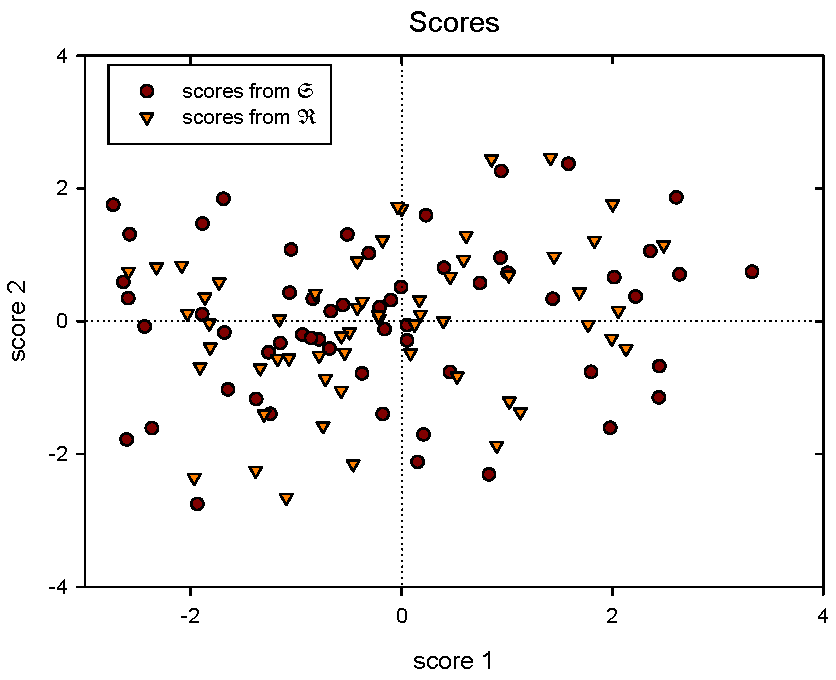
\includegraphics[width=0.75\textwidth]{Graphics/Scores-football}
\end{figure}

\vspace{5mm}

Varimax-rotation of these loadings proceeds in 5 steps for \arr{S} and 12 steps for \arr{R}. \\

{\footnotesize \begin{tabular}{r|rrrr|rrrr}
  \toprule
           & \multicolumn{4}{l} \arr{S} &  \multicolumn{4}{l} \arr{R}  \\
           & \(\AbsVec{l}_1 \) & \(\AbsVec{l}_2 \) & Commun & Uniq & \(\AbsVec{l}_1 \) & \(\AbsVec{l}_2 \) & Commun & Uniq \\
  \midrule
  WDIM     & 0.6753 & -0.0030 & 0.4561 & 0.5439  & 0.7289 &  0.1650 & 0.5586 & 0.4414 \\
  CIRCUM   & 0.9643 &  0.2421 & 0.9884 & 0.0116  & 0.9271 &  0.3746 & 0.9998 & 0.0002 \\
  FBEYE    & 0.8067 & -0.0882 & 0.6585 & 0.3415  & 0.7551 &  0.0318 & 0.5711 & 0.4289 \\
  EYEHD    & 0.1073 &  0.9842 & 0.9801 & 0.0199  & 0.2233 &  0.9329 & 0.9202 & 0.0798 \\
  EARHD    & 0.0086 &  0.4102 & 0.1684 & 0.8316  & 0.0915 &  0.6651 & 0.4507 & 0.5493 \\
  JAW      & 0.5286 & -0.1901 & 0.3156 & 0.6844  & 0.5902 & -0.1799 & 0.3807 & 0.6193 \\
  \midrule
  var acc  & 2.3277 &  1.2395 & 3.5672 & 2.4329  & 2.3676 &  1.5136 & 3.8811 & 2.1189 \\
  prop var & 0.3880 &  0.2066 & 0.5945 & 0.4055  & 0.3946 &  0.2523 & 0.6469 & 0.3532 \\
  \bottomrule
\end{tabular}}

\begin{figure}
   \caption{Unrotated and rotated loadings from the football-data }
   \label{fig:Loadings-football}
   \centering
      \includegraphics[width=0.75\textwidth]{Graphics/Loadings-football}
\end{figure}


\subsection{Interpretation}

How many variables should be included when interpreting a factor? According to \parencite{Gua-88} the following rules are supported by Monte Carlo simulation:
\begin{itemize}
  \item{when at least 4 variables load on a factor with at least 0.60, sample size is of little consequence}
  \item{when at least 10 variables load on a factor with at least 0.40, sample size is of little consequence}
  \item{If these conditions are not met, sample size should be at least 300}
  \item{If sample size is less than 300, random loading patterns may become relevant. The study should be reproduced. }
\end{itemize}

\printbibliography[heading=subbibliography]
\end{refsection}


  % -*- TeX:UK -*-
\chapter{Cluster-analysis}
\begin{refsection}


Cluster analysis is described in \parencite{Sne-73}, a very thorough yet readable introduction. We use the following definitions:
\begin{lstlisting}[caption=Program head]
  PROGRAM Similarity;

  USES math,            // Lazarus math unit
       MathFunc,        // general arithmetic
       Vector,          // vector arithmetic
       Matrix,          // matrix arithmetic
       BigSet,          // sets of arbitrary cardinality
       Correlations;    // correlation coefficients

  CONST MaxVariables =  180;
        MaxCases     = 1400;
        SepChar      =  ';';    // separates data IN csv-fles

  TYPE DataTypes  = (binary, nominal, ordinal, interval, rational);
       TypeVector = ARRAY[1..MaxVariables] OF DataTypes;

  VAR Types      : TypeVector;
      Data, Dist1, Dist2 : MatrixTyp;
      Variables,
      Cases,i,j  : WORD;
      r          : double;

  TYPE ClusterFeld = ARRAY [1..MaxCases] OF SetType;     // declarations should be local TO ClusterAnalysis

  VAR HilfsMatrix  : MatrixTyp;    { akt. Distanzen der Cluster oben, coph. Matrix unten und Clusterzustand diagonal }
      Cluster      : ClusterFeld;
      v            : VectorTyp;
\end{lstlisting}

\section{Read the data matrix}

The data are stored in a comma separated value (csv) file according to  \href{https://tools.ietf.org/html/rfc4180}{RFC 4180}, which can be exported from Excel. However, in Middle Europe the decimal separator is comma rather than point (as in the US), so that the semicolon is used as variable separator. The routine needs to handle this:
\begin{lstlisting}[caption=Read data from comma-separated file]
  PROCEDURE ReadCSV(VAR Cases, Variables : WORD; VAR Types: TypeVector;
                    VAR Data: MatrixTyp);

  CONST MaxCases = 200;

  VAR
    InputFile: TEXT;
    c: CHAR;
    s: STRING;
    Error, i, j: WORD;
    Interim: MatrixTyp;
    x: double;

  BEGIN
    Variables := 0;
    Cases := 0;
    Assign(InputFile, 'All.csv');
    Reset(InputFile);
    ReadLn(InputFile);            // ignore Line WITH variable names
    WHILE NOT EoLn(InputFile) DO  // Read data types from second Line, count Variables
    BEGIN
      INC(Variables);
      s := '';
      REPEAT
        Read(InputFile, c);
        IF c <> SepChar THEN
          S := s + c;
      UNTIL ((c = SepChar) OR EoLn(InputFile));
      CASE s OF
        'binary'   : Types[Variables] := binary;
        'ordinal'  : Types[Variables] := ordinal;
        'nominal'  : Types[Variables] := nominal;
        'interval' : Types[Variables] := interval;
        'rational' : Types[Variables] := rational
        ELSE
          BEGIN              // Format error: abort PROGRAM WITH error message
            Write('unknown data type ', s, ' at n=', Variables: 3, '. Press <CR>:');
            ReadLn;
            HALT;
         END; { else }
      END; { case }
    END; { while }
    ReadLn(InputFile);            // go TO next Line
    CreateMatrix(Interim, MaxCases, Variables, 0.0);  // Note: number OF persons NOT yet known
    WHILE NOT EoF(InputFile) DO   // now Read data from following lines AND count cases
      BEGIN
        INC(Cases);
        FOR i := 1 TO Variables DO
          BEGIN
            x := ReadFloat(InputFile);
            IF MathError
              THEN
                BEGIN
                  MathError := FALSE;
                  HALT;
                END;
            SetMatrixElement(Interim, Cases, i, x);
          END;
        ReadLn(InputFile);
      END; { while }
    Close(InputFile);
    CreateMatrix(Data, Cases, Variables, 0.0);  // now generate correctly sized data matrix
    FOR i := 1 TO Cases DO
      FOR j := 1 TO Variables DO
        SetMatrixElement(Data, i, j, GetMatrixElement(Interim, i, j));
    DestroyMatrix(Interim);                         // destroy the interim matrix
    Writeln(Cases: 4, ' cases with ', Variables: 3, ' variables read, ');
  END;
\end{lstlisting}

\section{Calculate the similarity/distance matrix}

A distance between two data points \(\AbsVec{x}_{i\cdot}, \AbsVec{x}_{j\cdot} \) is metric, if it meets the following conditions:
\begin{description}
  \item[non-negativity]{\( D(\AbsVec{x}_{i\cdot}, \AbsVec{x}_{j\cdot}) \geq 0 \)}
  \item[isolation]{\( D(\AbsVec{x}_{i\cdot}, \AbsVec{x}_{i\cdot}) = 0 \)}
  \item[symmetry]{\( D(\AbsVec{x}_{i\cdot}, \AbsVec{x}_{j\cdot}) = D(\AbsVec{x}_{j\cdot}, \AbsVec{x}_{i\cdot}) \)}
  \item[triangular inequality]{\( D(\AbsVec{x}_{i\cdot}, \AbsVec{x}_{j\cdot}) \geq D(\AbsVec{x}_{i\cdot}, \AbsVec{x}_{h\cdot}) + D(\AbsVec{x}_{h\cdot}, \AbsVec{x}_{j\cdot}) \) }
\end{description}
, and analogously for similarities.

Because we have data of mixed type we use the universal similarity coefficient of \Name{Gower} \parencite{Gow-71}, see also \parencite[chapter 4.4]{Sne-73}, which for two \textbf{individuals} \skalar{i, j} is defined as
\begin{equation}
  S_G = \frac{\sum_{k=1}^{p}{w_{i,j,k} s_{i,j,k}}}{\sum_{k=1}^{p}{w_{i,j,k}}}
\end{equation}
over all variables \skalar{k}. The \textbf{weight} \skalar{w_{i,j,k}} is set to \num{1} if a comparison on character \skalar{k} can be made for the individuals \skalar{i, j}, and \num{0} if such a comparison cannot be made (\Foreign{i.e.}, if at least one of the two data is missing). In that case, both denominator and numerator will increase by \num{0}, the data pair will be ignored. Thus, \skalar{S_G} is robust with respect to missing data. \skalar{s_{i,j,k}} is calculated depending on data type:
\begin{description}
  \item[binary]{\( \skalar{s_{i,j,k}} = 1 \) if both data are \num{1}, or \num{0} otherwise. If the data table consists of only binary variables, this would correspond to using \Name{Jaccard}'s coefficient (see page \pageref{tab:binary}). It is possible to have \(\skalar{s_{i,j,k}} = 1 \) also for negative matches, but this is rarely warranted and has negative statistical implications \parencite{Hub-82}.}
  \item[nominal]{\( \skalar{s_{i,j,k}} = 1 \) if the two data match, \num{0} otherwise. }
  \item[ordinal]{In the original publication \(\skalar{s_{i,j,k}} = 1 \) for match, \num{0} for mismatch. However, \parencite{Pod-99} suggested to rank the data and then use the ranks like cardinal values. This yields more information for each comparison. Because we already use numbers to encode ordinal data in the data table, this is easily accomplished. }
  \item[cardinal]{\( \skalar{s_{i,j,k}} = 1 - \frac{|X_{i,k} - X_{j,k}|}{R_k} \), with \skalar{R_k} the range of variable \skalar{k} (either range in the data set or, if known, range in the wild). This is the complement to the mean character difference of \parencite{Cai-58}.}
\end{description}
For clustering, we need distances rather than similarities, which is simply the complement to \num{1.0}.

\begin{lstlisting}[caption=Distance matrix]
  PROCEDURE Gowers(CONST Types : TypeVector; CONST Data : MatrixTyp;
                    VAR Dist : MatrixTyp);

  var SumW, i, j, k, Cases, Variables : word;
      S, SumWS, x, y          : double;
      Maximum, Minimum, Range : array [2..MaxVariables] of double; // as first column is case number

  begin
    Variables := MatrixColumns(Data);
    Cases     := MatrixRows(Data);
    for k := 2 to Variables do  // calculate range of intervall and rational data, ignore StudyNamber
      begin
        Maximum[k] := -MaxRealNumber;
        Minimum[k] := MaxRealNumber;
        case Types[k] of
          ordinal, interval, rational : begin
                for i := 1 to Cases do
                    begin
                      x := GetMatrixElement(Data, i, k);
                      if not isNaN(x)
                        then
                          begin
                            if (x > Maximum[k]) then Maximum[k] := x;
                            if (x < Minimum[k]) then Minimum[k] := x;
                          end;
                    end; { for i }
                  Range[k] := Maximum[k] - Minimum[k];
                end
          else Range[k] := 0.0;  // binary, nominal: just give it a defined value, won't be used
        END;  { case }
      END; { for k }
    Writeln('ranges calculated');
    Write('Distances: ');
    CreateIdentityMatrix(Dist, Cases);
    FOR i := 1 TO Cases DO
      BEGIN
        FOR j := Succ(i) TO Cases DO // calculate upper half OF similarity matrix
          BEGIN
             SumW := 0;
             SumWS := 0;
             FOR k := 2 TO Variables DO  // ignore CASE numbes
               BEGIN
                 x := GetMatrixElement(Data, i, k);
                 y := GetMatrixElement(Data, j, k);
  //               Write(OutFile, i:4, ';', j:4, ';', k:4, ';', FloatStr(x, 8), ';', FloatStr(y, 8), ';');
                 IF (isNaN(x) OR isNaN(y))
                   THEN // SumW AND SumWS both increase by 0
                   ELSE
                     CASE Types[k] OF
                       binary, nominal : BEGIN
                                           IF x = y
                                             THEN S := 0
                                             ELSE S := 1;
                                           INC(SumW);
                                           SumWS := SumWS + S; // AS W = 1 -> WS = S
                                         END;
                       ordinal, interval, rational :
                                         BEGIN
                                           S := Abs(x - y) / Range[k];
                                           INC(SumW);
                                           SumWS := SumWS + S;
                                         END;
                     END; { case }
               END; { for k }
             IF SumW = 0
               THEN x := NaN                     // so that such cases can be identified IN the distance matrix
               ELSE x := SumWS / SumW;
             SetMatrixElement(Dist, i, j, x);
             SetMatrixElement(Dist, j, i, SumW); // put number OF valid compares into lower half OF similarity matrix
          END;  { for j }
        IF (i MOD 20 = 0) THEN Write('.');
      END; { for i }
    Writeln(' calculated, ');
  END;  { Gowers }

  PROCEDURE WriteDistances (CONST Data, Dist : MatrixTyp);

  VAR i, j, cases  : WORD;
      OutFile : TEXT;
      MaxS, MinS, MaxC, MinC, x : double;

  BEGIN
    Cases := MatrixRows(Dist);
    Assign(OutFile, 'Distances.csv');
    Rewrite(OutFile);
    MaxS := MinRealNumber;
    MaxC := MinRealNumber;
    MinS := MaxRealNumber;
    MinC := MaxRealNumber;
    Write(OutFile, 'StudyNum;');  // LABEL columns
    FOR i := 1 TO Cases DO Write(OutFile, Round(GetMatrixElement(Data, i, 1)):4, ';');
    Writeln(OutFile);
    FOR i := 1 TO Cases DO // the matrix itself
      BEGIN
        Write(OutFile, Round(GetMatrixElement(Data, i, 1)):4, ';');
        FOR j := 1 TO Cases DO
          IF (j>i)
            THEN
              BEGIN
                x := GetMatrixElement(Dist, i, j);
                Write(OutFile, x:6:4, ';');   // upper half WITH similarity
                IF IsNaN(x)
                  THEN
                  ELSE
                    BEGIN
                      IF (x > MaxS) THEN MaxS := x;
                      IF (x < MinS) THEN MinS := x;
                    END;
              END
            ELSE
               BEGIN
                x := GetMatrixElement(Dist, i, j);
                Write(OutFile, Round(x):4, ';');  // lower half WITH # OF comparisons
                IF (j < i) // ignore i=j
                  THEN
                    BEGIN
                      IF (x > MaxC) THEN MaxC := x;
                      IF (x < MinC) THEN MinC := x;
                    END;
              END;
         Writeln(OutFile)
      END;  { for i }
    Close(OutFile);
    Writeln;
    Writeln('Distances written to file, ');
    Writeln('Range ', MinS:5:3, '-', MaxS:5:3, ' with ', MinC:3:0, '-', MaxC:3:0, ' comparisons');
  END; { WriteDistances }

  PROCEDURE AnalyseFrequencies(CONST Dist: MatrixTyp);

  CONST Border = 50;    // number OF ranges FOR statistical analysis OF correlations

  TYPE FreqsType  = ARRAY[-Border..Border] OF WORD;

  VAR
    i, j, Cases     : WORD;
    k               : INTEGER;
    OutFile         : TEXT;
    x               : double;
    Freqs           : FreqsType;

  BEGIN
    Assign(OutFile, 'DistFreq.csv');
    Rewrite(OutFile);
    Cases := MatrixRows(Dist);
    FOR k := -Border TO Border DO
      Freqs[k] := 0;
    FOR i := 1 TO Cases DO
      FOR j := Succ(i) TO Cases DO
      BEGIN
        x := GetMatrixElement(Dist, i, j) * Border;
        INC(Freqs[Round(x)]);
      END;
    FOR k := -Border TO Border DO
       Writeln(OutFile, k/Border:1:4, SepChar, Freqs[k]:6, SepChar);
    Writeln(OutFile);
    Close(OutFile);
  END;
\end{lstlisting}

\section{Hierarchic-agglomerative clustering}

A cluster is a set of \textbf{\acf{OTU}s} that were combined at a certain similarity. Initially, each \acs{OTU} forms a cluster by itself, then in each step the most similar clusters are combined and the process is continued until all \acs{OTU}s have been combined in a single cluster. The result is a binary tree. The similarity of two clusters is calculated as the unweighed average of the similarities of all members of one cluster with all members of the other (average linkage, \textbf{\acf{UPGMA}}). Alternatively, the distance between the most distant (complete linkage) or the closest \acs{OTU}s () of the clusters may be used, however, clustering tends to be better with average linkage.

The routine returns the \textbf{cophenetic correlation coefficient}, which describes how well the tree preserves the pairwise distance of the \acs{OTU}s.

\begin{lstlisting}[caption=clustering]
  FUNCTION ClusterAnalysis (CONST Dist : MatrixTyp) : double;

  VAR i, j,
      AnzCluster   : WORD;
      MinAbst      : double;
      ClusterDatei : TEXT;

       PROCEDURE Minimum (CONST HilfsMatrix : MatrixTyp; VAR MinAbst : double);

       VAR i, j     : WORD;

       BEGIN
         FOR i := 1 TO Pred(Cases) DO
           FOR j := Succ(i) TO Cases DO
             IF GetMatrixElement(HilfsMatrix, i, j) < MinAbst
               THEN MinAbst := GetMatrixElement(HilfsMatrix, i, j);
     END;


       PROCEDURE UniteCluster (VAR Cluster : ClusterFeld; i, j : WORD; MinAbst : double);

       VAR k : WORD;

       BEGIN
         SetUnion(Cluster[i], Cluster[i], Cluster[j]);
         ClearAllBits(Cluster[j]);
         Writeln(ClusterDatei);
         Writeln;
         Write(ClusterDatei, MinAbst:6:4, ' ');
         Write(MinAbst:6:4, ' ');
         FOR k := 1 TO Cases DO
           IF InSet(Cluster[i], k)
             THEN
               BEGIN
                 Write(ClusterDatei, Round(GetMatrixElement(Data, k, 1)):4, ' ');
                 Write(Round(GetMatrixElement(Data, k, 1)):4, ' ');
               END;
         Writeln(ClusterDatei);
         Writeln;
       END;


       PROCEDURE Cophen (VAR HilfsMatrix : MatrixTyp; CONST Cluster : ClusterFeld;
                         MinAbst : double);

       VAR i, j, l : WORD;

       BEGIN
         FOR i := 1 TO Cases DO
           IF NOT EmptySet(Cluster[i])
             THEN
               FOR j := 1 TO Pred(Cases) DO
                  IF InSet(Cluster[i], j)
                    THEN
                      FOR l := Succ(i) TO Cases DO
                         IF InSet(Cluster[i], l)
                           THEN
                             IF (GetMatrixElement(HilfsMatrix, l, j) = 0)
                               THEN SetMatrixElement(HilfsMatrix, l, j, MinAbst);
       END; { Cophen }


       PROCEDURE NewDistances (CONST Cluster : ClusterFeld; CONST Dist : MatrixTyp;
                                  VAR HilfsMatrix : MatrixTyp);

       VAR i, j, k, l, b : WORD;
           a             : double;

       BEGIN
         FOR i := 1 TO Pred(Cases) DO
           FOR j := Succ(i) TO Cases DO
             BEGIN
               IF ((NOT EmptySet(Cluster[i])) AND (NOT EmptySet(Cluster[j])))
                 THEN
                   BEGIN
                     a := 0.0;
                     b := 0;
                     FOR k := 1 TO Cases DO
                       IF InSet(Cluster[i], k)
                         THEN
                           FOR l := 1 TO Cases DO
                             IF InSet(Cluster[j], l)
                               THEN
                                 BEGIN
                                   a := a + GetMatrixElement(Dist, k, l);
                                   INC(b);
                                 END;
                     SetMatrixElement(HilfsMatrix, i, j, a/b);
                   END
                 ELSE
                   SetMatrixElement(HilfsMatrix, i, j, MaxInt);
             END; { for }
       END; {NeueSimularitaeten}


       FUNCTION NewDiagonal (CONST Cluster: ClusterFeld; VAR HilfsMatrix : MatrixTyp) : WORD;

       VAR i, j : WORD;

       BEGIN
         j := 0;
         FOR i := 1 TO Cases DO
           IF NOT EmptySet(Cluster[i])
             THEN
               BEGIN
                 SetMatrixElement(HilfsMatrix, i, i, 1);
                 INC(j);
               END
             ELSE
               SetMatrixElement(HilfsMatrix, i, i, 0);
         NewDiagonal := j;
       END;


       FUNCTION Correlation (CONST Dist, HilfsMatrix : MatrixTyp) : double;

       VAR DistMittel, CoMittel,
           DistKor, CoKor,
           SumDistKorSqr, SumCoKorSqr,
           SumDistKorCoKor             : double;


           PROCEDURE Mittelwerte (CONST Dist, HilfsMatrix : MatrixTyp);

           VAR SumDist, SumCo : double;
               i, j, z       : WORD;

           BEGIN
             SumDist := 0;
             SumCo := 0;
             z := 0;
             FOR i := 1 TO Pred(Cases) DO
               FOR j := Succ(i) TO Cases DO
                 BEGIN
                   SumDist := SumDist + GetMatrixElement(Dist, i, j);
                   SumCo := SumCo + GetMatrixElement(HilfsMatrix, j, i);
                   INC(z);
                 END;
             DistMittel := SumDist / z;
             CoMittel := SumCo / z;
           END;


           FUNCTION Summen (CONST Dist, HilfsMatrix : MatrixTyp) : double;

           VAR i, j : WORD;

           BEGIN
             SumDistKorSqr := 0;
             SumCoKorSqr := 0;
             SumDistKorCoKor := 0;
             FOR i := 1 TO Pred(Cases) DO
               FOR j := Succ(i) TO Cases DO
                 BEGIN
                   DistKor := GetMatrixElement(Dist, i, j) - DistMittel;
                   CoKor := GetMatrixElement(HilfsMatrix, j, i) - CoMittel;
                   SumDistKorSqr := SumDistKorSqr + Sqr(DistKor);
                   SumCoKorSqr := SumCoKorSqr + Sqr(CoKor);
                   SumDistKorCoKor := SumDistKorCoKor + DistKor * CoKor;
                 END;
             Writeln(SumDistKorCoKor:4:1, ' ', SumDistKorSqr:4:1, ' ',  SumCoKorSqr:4:1);
             Summen := SumDistKorCoKor / (Sqrt(SumDistKorSqr) * Sqrt(SumCoKorSqr));
           END;

       BEGIN
         Mittelwerte(Dist, HilfsMatrix);
         Correlation := Summen(Dist, HilfsMatrix);
       END;

  BEGIN
    ClusterAnalysis := 0.0;
    Assign(ClusterDatei, 'Similarities.CLU');
    Rewrite(ClusterDatei);
    CopyMatrix(Dist, HilfsMatrix);
    FOR i := 1 TO Cases DO         // jedem OTU sein eigenes Cluster
      BEGIN
        ClearAllBits(Cluster[i]);
        SetBit(Cluster[i], i);
      END;
    REPEAT                                        { Beginn der Analysenschleife }
      MinAbst := MaxRealNumber;
      Minimum(HilfsMatrix, MinAbst);
      FOR i := 1 TO Pred(Cases) DO               { neue Cluster bilden }
        FOR j := Succ(i) TO Cases DO
          IF (GetMatrixElement(HilfsMatrix, i, j) = MinAbst)
            THEN UniteCluster(Cluster, i, j, MinAbst);
      Cophen(HilfsMatrix, Cluster, MinAbst);
      NewDistances(Cluster, Dist, HilfsMatrix);
      AnzCluster := NewDiagonal(Cluster, HilfsMatrix);
    UNTIL AnzCluster = 1;
    Close(ClusterDatei);
    Result := Correlation(Dist, Hilfsmatrix);
  END;
\end{lstlisting}

\begin{lstlisting}[caption=compare distance matrices]
  FUNCTION MatrixCorrelation (CONST Dist1, Dist2 : MatrixTyp) : float;

  VAR i, j, k : WORD;
    SumXY, SumX, SumY, SumX2, SumY2, varX, varY, covXY, x, y, r : float;
    OutFile : TEXT;

  BEGIN
    Assign(OutFile, 'DistCorr.csv');
    Rewrite(OutFile);
    Cases := MatrixRows(Dist1);
    SumXY := 0;
    SumX := 0;
    SumY := 0;
    SumX2 := 0;
    SumY2 := 0;
    k := 0;
    FOR i := 1 TO Cases DO
      FOR j := Succ(i) TO Cases DO
        BEGIN
          x := GetMatrixElement(Dist1, i, j);
          y := GetMatrixElement(Dist2, i, j);
          Writeln(OutFile, i:3, ';', j:3, ';', FloatStr(x, 10), ';', FloatStr(y, 10), ';');
          SumXY := SumXY + x * y;
          SumX := SumX + x;
          SumY := SumY + y;
          SumX2 := SumX2 + x * x;
          SumY2 := SumY2 + y * y;
          INC(k); // actual number OF valid comparisons
         END; { for }
    varX := k * SumX2 - SumX * SumX;
    varY := k * SumY2 - SumY * SumY;
    covXY := k * SumXY - SumX * SumY;
    IF Abs(varX * varY) < Zero
      THEN Result := 0     // ???
      ELSE Result := covXY / Sqrt(varX * varY);
    Writeln(OutFile, FloatStr(Result, 10));
    Close(OutFile);
  END; { MatrixCorrelation }
\end{lstlisting}


The main part of the program is then quite short:

\begin{lstlisting}[caption=Main program]
  BEGIN
    ReadCSV (Cases, Variables, Types, Data);
    Gowers(Types, Data, Dist1);
    CalcCaseCorrelations(Data, Dist2);
    WriteDistances(Data, Dist2); // Data IS source OF study-number
    AnalyseFrequencies(Dist2);
    FOR i := 1 TO Cases DO
       FOR j := Succ(i) TO Cases DO
         BEGIN
           SetMatrixElement(Dist1, j, i, GetMatrixElement(Dist1, i, j));       // symmetrieren
           SetMatrixElement(Dist2, j, i, GetMatrixElement(Dist2, i, j));
         END;
    LeadingPrincipleMinors(Dist2, V);
    FOR i := 1 TO Cases DO
      Writeln(FloatStr(GetVectorElement(V, i), 10));
    DestroyVector(V);
    r := MatrixCorrelation (Dist1, Dist2);
    r := ClusterAnalysis(Dist2);
    Write('Cophenetic correlation', r:1:3, ' Press <CR> to finish:');
    ReadLn;
  END.
\end{lstlisting}

\section{\skalar{k}-means clustering}

The data (which need to be cardinal) are grouped into \skalar{k} clusters \( \arr{C}_i \), where \(i \in [1..k], k \ll n \) is a number that must be chosen at the begin of the study. The algorithm is as follows \parencite{McQ-67, Har-79}:
\begin{enumerate}
   \item{Randomly select \skalar{k} \acs{OTU}s as centres of the clusters, and assign each \acs{OTU} to the closest centre (by squared \Name{Euklid}ian distance).}
   \item{Repeat
     \begin{enumerate}
        \item{Calculate the centroids of all clusters, that is, the vector of the \skalar{p} feature means for the observations in the \skalar{i}th cluster. }
        \item{Assign each \acs{OTU} to the cluster whose centroid is closest}
     \end{enumerate}
     until OTUs are no longer assigned to different centres. }
\end{enumerate}
This partitions the data space into \Name{Voronoi} cells. Should a cluster become empty, a new centre needs to be chosen. In effect, the between-cluster distances are maximised, the within-cluster distance minimised.

Finding optimal partitioning (minimal sum of squared distances from the centres \( \sum_{i=1}^k \sum_{\AbsVec{x} \in \arr{C}_i}{\mathrm{dist}(\AbsVec{c}_i, \AbsVec{x})^2} \)) is NP-hard, the result of above heuristic depends somewhat on the starting assignments, the program needs to be run several times. Finally, the best solution is chosen. The algorithm is \( \mathbf{O}(npkm) \), where \skalar{m} is the number of iterations required. Local optima can be left by swapping \acs{OTU}s between clusters. Missing data can be handled by imputation of a probable range \parencite{Li-16}.


\subsection{Modifications}

\begin{description}
  \item[\skalar{k}-means++ algorithm]{selects one \acs{OTU} randomly as starting point. Then the distances of all \acs{OTU}s to this starting point are calculated, and the next centre is determined so that the probability of an \acs{OTU} to become the centre depends on the square of the distance to the original starting point. This is repeated until all \skalar{k} centres have been selected. Then perform the \skalar{k}-means algorithm. This method converges twice as fast as the simple \skalar{k}-means algorithm, with similar end results.}
  \item[\skalar{k}-median algorithm]{uses medians instead of means and Manhatten-distances \skalar{\ell_1} (absolute value of difference) instead of \Name{Euklid}ian \skalar{\ell_2} (squared distance, see section \ref{text:Norm} on page \pageref{text:Norm}).}
  \item[\acf{PAM} algorithm]{tries to minimise the distance of the data points from the medoid instead of the centroid. While the centroid as mean of the data is synthetic, the medoid is a member of the data set that represents its group \parencite{Kau-90}. Since the calculation of means is sensitive to outliers, \acs{PAM} is more robust than \skalar{k}-means clustering. \skalar{k} data vectors are randomly assigned as medoids, other data points are assigned to their closest medoid. Then data and medoids are exchanged to minimise an objective (= distance) function.}
  \item[\skalar{k}-modes clustering]{can handle categorical data. The distance of an \acs{OTU} to the centre of a cluster is given by the sum over all \skalar{p} variables of 1 for mismatches and \( 1 - \frac{n^r_j}{n_j} \) for matches, that is, matches for rare categories are weighted heavier than matches of frequent ones. Mixed categorical/cardinal data can be handled with universal distance functions like \Name{Gower}'s. }
  \item[kernel \skalar{k}-means]{is used for data that are not linearly separable. Kernel methods try to classify cases by transforming the data into higher dimensions. }
  \item[expectation–maximization algorithm]{is a generalisation of \skalar{k}-means clustering that works even if the clusters have very different sizes, densities or non-spherical shape. However, it is much more complex.}
\end{description}


\subsection{Selection of optimal \skalar{k}}

\subsubsection{Elbow-method}

For all \skalar{k}, calculate the within-cluster sum of square (wss) and plot against \skalar{k}. The optimal \skalar{k} is the position of the elbow in the plot (similar to scree-plot in \acs{PCA}, see section \ref{text:scree} on page \pageref{text:scree}).

\subsubsection{Average silhouette method}

A silhouette \( S(\AbsVec{x}) \) is a measure how close an observation \( \AbsVec{x}_{i\cdot} \) is to the nearest two clusters, and thus a measure of the quality of clustering. The average distance between an observation and a cluster \( \arr{C}_i \) is defined as the arithmetic average of the distances of \( \AbsVec{x}_{i\cdot} \) to all (other) members of \( \arr{C}_i \). Then
\begin{equation}
  S(\AbsVec{x}) = \left\{
                    \begin{array}{c@{\;}c}
                       0 & \mathrm{if\ \AbsVec{x}_{i\cdot} is\ the\ only\ element\ of\ \arr{C}_i} \\
                       \frac{\dist(\AbsVec{x}_{i\cdot}, \arr{C}_i)-\dist(\AbsVec{x}_{i\cdot}, \arr{C}_j)}{\max(\dist(\AbsVec{x}_{i\cdot}, \arr{C}_i), \dist(\AbsVec{x}_{i\cdot}, \arr{C}_j))} & \mathrm{else}
                    \end{array}
                 \right.
\end{equation}
\skalar{s(\arr{C}_i)} is the arithmetic mean of all silhouettes of the  cluster \( \arr{C}_i \). If it is close to +1, the data point is in the appropriate cluster, if it is \num{-1}, it should be a member of the neighbouring cluster. A value near zero indicates that \( \AbsVec{x}_{i\cdot} \) is close to the border between clusters. The mean of all \skalar{s(\arr{C}_i)} of \( \arr{C}_i \) indicates how tightly grouped all the points in the cluster are. The mean \skalar{s(\arr{C}_i)} over all data is a measure of how well the data have been clustered. The silhouette coefficient is the largest \skalar{s(\arr{C}_i)} over all data in the entire data set. This can be used as criterium for optimising \skalar{k}.

The cluster (of which \( \AbsVec{x}_{i\cdot} \) is not a member) with minimal \( S(\AbsVec{x}) \) is said to be the neighboring cluster.

The silhouette plot plots a line of length \skalar{S(\AbsVec{x})} for all elements of the cluster, in descending order.


\subsubsection{Gap statistics}

Here we compare the within-cluster sum of square with that obtained on a synthetic data set with random data, which have the same range (\(\min{(\AbsVec{x}_{\cdot j})}, \max{(\AbsVec{x}_{\cdot j})}\)) as the original data set (bootstrapping). Then for \skalar{B} artificial data sets, calculate average and standard deviation of the logarithms of wss and plot \( \mathrm{Gap}(\skalar{k}) = \overline{\log(\mathrm{wss})_B} - \log(\mathrm{wss}_k) \) as function of \skalar{k}. Then \( s_k = \mathrm{sd}_k \times \sqrt{1 + 1/B} \) and we look for the smallest \skalar{k} where Gap(\skalar{k}) \(\geq\) Gap(\skalar{k}+1) - \skalar{s_{k+1}}.

\subsection{Sourcecode for \skalar{k}-means clustering with \skalar{k}-fold crossvalidation}

\subsubsection{\skalar{k}-means clustering}

\begin{lstlisting}[caption=unit kNN: \skalar{k}-means clustering]
  UNIT kNN;

  INTERFACE

  USES Math,
       MathFunc,
       Vector,
       Matrix,
       Deskript,
       Zufall,
       CrossValidation;

  CONST
    kNNError: BOOLEAN = FALSE;
    KNNmax = 15;
    pMax = 100;

  TYPE
    GroupTyp = ARRAY[1..MaxVector] OF WORD;

  FUNCTION kMeansCluster(CONST Data: MatrixTyp;       // data matrix
    k: WORD;                                          // number OF clusters
    VAR Centroids: MatrixTyp;                         // centroids FOR all k clusters AND p variables
    VAR Group: GroupTyp): float;                      // group no FOR each item
  { splits a data matrix into k groups by the k-nearest neighbour method and
    returns the sum of Euklidian distances of the data from their centroids. }

  PROCEDURE AssignTestData(CONST TestData, Centroids: MatrixTyp;
    kValidate : WORD;                                         // number OF cross-validation groups
    VAR Count : WORD;                                         // no OF results calculated already
    VAR ValidationResult: MatrixTyp);                         // Result
  { assigns all rows of Data to the closest Centroid and
    returns the study number, assigned group and squared distance to the centroid
    in ValidationResult }

  FUNCTION WithinSumOfSquares(CONST ValidationResult: MatrixTyp): float;
  { calculates the sum of the squared distance of all data from their centroid,
    which is stored in the third column of ValidationResult }

  IMPLEMENTATION

  PROCEDURE StartingCentoids(CONST Data: MatrixTyp; k: WORD; VAR Centroids: MatrixTyp);
  // select the starting centroids using knn++ METHOD (distance-controlled Random)

  VAR
    v, vi, row, Distance : VectorTyp;
    i, j, l, n, p        : WORD;
    r                    : LONGINT;
    Used                 : ARRAY[1..KNNmax] OF WORD;
    u                    : BOOLEAN;
    c                    : CHAR;
    d, Sum               : float;

  BEGIN
    n := MatrixRows(Data);
    p := MatrixColumns(Data);
    CreateMatrix(Centroids, k, p, 0.0);
    i := RandomLaplace(1, n);          // randomly select first centroid
    Writeln('first centroid = ', i: 3);
    GetRow(Data, i, v);
    SetRow(Centroids, v, 1);
    Used[1] := i;
    FOR j := 2 TO k DO                        // select the remaining centroids
      BEGIN
        CreateVector(Distance, n, 0.0);
        IF VectorError
          THEN
            BEGIN
              c := WriteErrorMessage('program terminated');
              HALT;
            END;
        Sum := 0;
        FOR i := 1 TO n DO // calculate distance between all items AND last centroid
          BEGIN
            GetRow(Data, i, vi);
            d := SquaredEuklidianDistance(v, vi, TRUE);
            DestroyVector(vi);
            SetVectorElement(Distance, i, d);
            FOR l := 1 TO Pred(j) DO          // ignore IF datum i IS already a centroid
              IF Used[l] = i THEN u := TRUE;
            IF NOT (u) THEN Sum := Sum + d;
          END;
        l := ceil(Sum);
        r := RandomLaplace(1, l); // distance-controlled Random selection OF NEW centroid
        Sum := 0;
        i := 0;
        REPEAT
          INC(i);
          u := FALSE;
          FOR l := 1 TO Pred(j) DO
            IF Used[l] = i THEN u := TRUE;
          IF NOT (u) THEN Sum := sum + Round(GetVectorElement(Distance, i));
        UNTIL (Sum >= r);
        GetRow(Data, i, vi);
        SetRow(Centroids, vi, j);
        FOR i := 1 TO p DO
          SetVectorElement(v, i, GetVectorElement(vi, i));
        DestroyVector(vi);
        DestroyVector(Distance);
      END; // FOR j
    DestroyVector(v);
  END;  // StartingCentroids

  FUNCTION AssignItems(CONST Data, Centroids: MatrixTyp;
    k: WORD;
    VAR Group: GroupTyp): float;
    // Assign each datum TO the cluster from the centre OF which it has minimal
    // distance. Returns sum OF the minimal distances over all data

  VAR
    i, j, l, n, p : WORD;
    d, min, Sum   : float;
    vj, vi        : VectorTyp;

  BEGIN
    n := MatrixRows(Data);
    p := MatrixColumns(Data);
    Sum := 0;
    FOR i := 1 TO n DO             // FOR all data rows
      BEGIN
        min := MaxRealNumber;
        GetRow(Data, i, vi);
        FOR j := 1 TO k DO         // find centroid WITH minimal distance TO the datum
        BEGIN
          GetRow(Centroids, j, vj);
          d := SquaredEuklidianDistance(vj, vi, TRUE);
          IF (d < min)
            THEN
              BEGIN
                min := d;
                l := j;
              END; // THEN
          DestroyVector(vj);
        END; // FOR j
        Group[i] := l;
        Sum := Sum + min;
        DestroyVector(vi);
      END; // FOR i
    Result := Sum;
  END; // AssignItems


  PROCEDURE CalculateNewCentroids(CONST Data: MatrixTyp;
    k: WORD;
    VAR Group: GroupTyp;
    VAR Centroids: MatrixTyp
    );

  VAR
    i, j, l, n, p, nk : WORD;
    Sums              : ARRAY [1..pMax] OF float;
    x                 : float;

  BEGIN
    n := MatrixRows(Data);
    p := MatrixColumns(Data);
    FOR l := 1 TO k DO
      BEGIN
        FOR j := 1 TO p DO
          Sums[j] := 0.0;
        nk := 0;
        FOR i := 1 TO n DO
          BEGIN
            IF Group[i] = l
              THEN
                BEGIN
                  FOR j := 1 TO p DO
                    BEGIN
                      x := GetMatrixElement(Data, i, j);
                      Sums[j] := Sums[j] + x;
                    END;
                END;
            INC(nk);
          END;
        FOR j := 1 TO p DO
          IF (nk = 0)
            THEN
              SetMatrixElement(Centroids, k, j, 0) // no data IN group, shouldn't happen
            ELSE
              SetMatrixElement(Centroids, k, j, Sums[j] / nk);
      END; // for l
  END; // CalculateNewCentroids


  FUNCTION kMeansCluster(CONST Data: MatrixTyp;
    k: WORD;
    VAR Centroids: MatrixTyp;
    VAR Group: GroupTyp): float;

  VAR
    p, n, Iter         : WORD;
    TotalDist, OldDist : float;

  BEGIN  // kMeansCluster
    n := MatrixRows(Data);
    p := MatrixColumns(Data);
    StartingCentoids(Data, k, Centroids);
    TotalDist := MaxRealNumber;
    Iter := 0;
    REPEAT
      OldDist := TotalDist;
      Inc(Iter);
      TotalDist := AssignItems(Data, Centroids, k, Group);
      CalculateNewCentroids(Data, k, Group, Centroids);
    UNTIL (abs(OldDist - TotalDist) < MaxError) OR (Iter > MaxIter);
    Result := TotalDist;
  END;   // kMeansCluster

  PROCEDURE AssignTestData(CONST TestData, Centroids: MatrixTyp;
    kValidate : WORD;
    VAR Count : WORD;
    VAR ValidationResult: MatrixTyp);

  VAR
    i, j, k, n, p, Opt : WORD;
    vi, vj             : VectorTyp;
    d, MinD            : float;

  BEGIN
    n := MatrixRows(TestData);
    p := MatrixColumns(TestData);
    k := MatrixRows(Centroids);
    CreateVector(vi, p, 0.0);
    FOR i := 1 TO n DO       // for all data in test data matrix
      BEGIN
        GetRow(TestData, i, vi);
        MinD := MaxRealNumber;
        Opt := 0;
        FOR j := 1 TO k DO  // find centroid of minimal distance
          BEGIN
            GetRow(Centroids, j, vj);
            d := SquaredEuklidianDistance(vi, vj, True);
            IF d < MinD
              THEN
                BEGIN
                  MinD := d;
                  Opt := j;
                END; // then
            DestroyVector(vj);
          END; // for j
        SetMatrixElement(ValidationResult, Count, 1, GetMatrixElement(TestData, i, 1));
        // study number
        SetMatrixElement(ValidationResult, Count, 2, Opt);  // optimal centroid
        SetMatrixElement(ValidationResult, Count, 3, MinD); // distance from centroid
        DestroyVector(vi);
        INC(Count);
      END; // for i
  END; // AssignTestData


  FUNCTION WithinSumOfSquares(CONST ValidationResult: MatrixTyp): float;

  VAR
    i, n: WORD;
    WSS: float;

  BEGIN
    n := MatrixRows(ValidationResult);
    WSS := 0;
    FOR i := 1 TO n DO
      WSS := WSS + GetMatrixElement(ValidationResult, i, 3);
    Result := WSS;
  END;  // WithinSumOfSquares

  end. //kNN
\end{lstlisting}

\subsubsection{\skalar{k}-fold crossvalidation}

\begin{lstlisting}[caption=k-fold crossvalidation]
  UNIT CrossValidation;

  INTERFACE

  USES MathFunc, Vector, Matrix, Zufall;

  CONST
    MaxK = 15;
    CrossValidationError: BOOLEAN = FALSE;

  TYPE
    SplitDataTyp = ARRAY [1..MaxK] OF MatrixTyp;


  PROCEDURE SplitDataMatrix(CONST Data: MatrixTyp;   // data matrix
    kValidate: WORD;                                 // no OF validation groups
    VAR SplitData: SplitDataTyp);                    // randomly distributed data
  { randomly splits the data matrix into kValidate sub-matrices }

  PROCEDURE CreateTestData(CONST SplitData: SplitDataTyp;
    k, kValidate: WORD;
    VAR TestData: MatrixTyp);
  { combine all Groups except the out of box group k into test matrix }


  IMPLEMENTATION

  PROCEDURE SplitDataMatrix(CONST Data: MatrixTyp; kValidate: WORD;
                            VAR SplitData: SplitDataTyp);

  VAR
    h, i, j, n, p : WORD;
    c             : CHAR;
    Available     : ARRAY [1..MaxK] OF WORD;
    CurrentRow    : VectorTyp;

  BEGIN
    IF (kValidate > MaxK)
      THEN
        BEGIN
          CrossValidationError := TRUE;
          c := WriteErrorMessage('k-fold cross-validation: kValidate > maximum');
          EXIT;
        END;
    n := MatrixRows(Data);
    p := MatrixColumns(Data);
    j := n DIV kValidate;  // number OF elements OF all submatrices except last
    FOR i := 1 TO Pred(kValidate) DO
      BEGIN
        CreateMatrix(SplitData[i], j, p, 0.0);
        IF MatrixError
          THEN
            BEGIN
              CrossValidationError := TRUE;
              MatrixError := FALSE;
              c := WriteErrorMessage('k-fold cross-validation: not enough memory');
              EXIT;
            END;
        Available[i] := j;
      END;
    CreateMatrix(SplitData[kValidate], j + (n MOD kValidate), p, 0.0);
    // put left-overs into last group
    IF MatrixError
      THEN
        BEGIN
          CrossValidationError := TRUE;
          MatrixError := FALSE;
          c := WriteErrorMessage('k-fold cross-validation: not enough memory');
          EXIT;
        END;
    Available[kValidate] := j + (n MOD kValidate);
    FOR i := 1 TO n DO // randomly put each data row into one OF the kValidate submatrices
      BEGIN
        REPEAT
          j := Round(RandomLaplace(1, kValidate)); // select group
        UNTIL (Available[j] > 0);
        GetRow(Data, i, CurrentRow);
        h := Succ(MatrixRows(SplitData[j]) - Available[j]);
        SetRow(SplitData[j], CurrentRow, h);
        DEC(Available[j]);
        DestroyVector(CurrentRow);
      END;
  END; { SplitDataMatrix }

  PROCEDURE CreateTestData(CONST SplitData: SplitDataTyp; k, kValidate: WORD;
                           VAR TestData: MatrixTyp);

  VAR
    j, n, p, Sum : WORD;
    i            : 1..MaxK;
    v            : VectorTyp;
    c            : CHAR;

  BEGIN
    Sum := 0;
    FOR i := 1 TO kValidate DO  // calculate number OF rows OF TEST data
      IF i <> k
        THEN
          BEGIN
            n := MatrixRows(SplitData[i]);
            Sum := Sum + n;
          END;
    p := MatrixColumns(SplitData[1]);
    CreateMatrix(TestData, Sum, p, 0.0);
    IF MatrixError
      THEN
        BEGIN
          CrossValidationError := TRUE;
          MatrixError := FALSE;
          c := WriteErrorMessage('k-fold cross-validation: not enough memory');
          EXIT;
        END;
    Sum := 0;
    FOR i := 1 TO kValidate DO
      IF i <> k
        THEN
          BEGIN
            FOR j := 1 TO MatrixRows(SplitData[i]) DO
              BEGIN
                INC(Sum);
                GetRow(SplitData[i], j, v);
                SetRow(TestData, v, Sum);
                DestroyVector(v);
              END;
          END;
  END; { CreateTestData }

  END.
\end{lstlisting}

\subsubsection{Main program}

\begin{lstlisting}[caption=Main program]
  PROGRAM kNNTest;

  USES
    Math,            // free pascal standard math UNIT
    MathFunc,        // basic math routines
    Vector,          // vector algebra
    Matrix,          // matrix algebra
    Zufall,          // Random numbers
    Deskript,        // descriptive statistics
    kNN,             // k means clustering
    CrossValidation  // k-fold cross-validation
    ;

  CONST
    n = 112;     // data sets
    p = 23;      // variables

  VAR
    Data, ValidationResult, TestData, Centroids : MatrixTyp;
    SplitData                                   : SplitDataTyp;
    i, j, k, l, kValidate, kmeans, done, Count  : WORD;
    c                                           : CHAR;
    Distance                                    : float;
    Group                                       : GroupTyp;
    WSS                                         : ARRAY[1..kNNmax] OF float;

    PROCEDURE ReadCSV(n, p: WORD; FileName: STRING; VAR Data: MatrixTyp);
    // Read correlation matrix from CSV FILE

    VAR
      InputFile : TEXT;
      i, j      : WORD;
      x         : float;
      c         : CHAR;

    BEGIN
      Assign(InputFile, Filename);
      Reset(InputFile);
      IF IOResult <> 0
        THEN
          BEGIN
            c := WriteErrorMessage('Unable to open file, Press <CR>');
            HALT;
          END;
      ReadLn(InputFile);            // ignore first Line WITH headers
      ReadLn(InputFile);            // ignore second Line WITH types
      CreateMatrix(Data, n, p, 0.0);
      IF MatrixError
        THEN
          BEGIN
            c := WriteErrorMessage('program terminated');
            HALT;
          END;
      FOR i := 1 TO n DO            // now Read data from following lines
        BEGIN
          FOR j := 1 TO p DO
            BEGIN
              x := ReadFloat(InputFile);
              IF MathError
                THEN
                  BEGIN
                    c := WriteErrorMessage('Unable to read datum, press <CR>');
                    HALT;
                  END;
              SetMatrixElement(Data, i, j, x);
            END; { for j }
          ReadLn(InputFile);
        END; { for i }
      Close(InputFile);
    END; { ReadCSV }


  BEGIN
    k := 2;
    ReadCSV(n, p, 'All.csv', Data);
    ShellSortMatrix(Data, 1);
    // ensure that data are sorted by study no
    kValidate := floor(Sqrt(n));                   // groups FOR k-fold cross-validation
    IF kValidate > MaxK THEN kValidate := MaxK;
    SplitDataMatrix(Data, kValidate, SplitData);
    IF CrossValidationError
      THEN
        BEGIN
          c := WriteErrorMessage('program terminated');
          HALT;
        END;
    CreateMatrix(ValidationResult, n, 3, 0.0);
    IF MatrixError
      THEN
        BEGIN
          c := WriteErrorMessage('program terminated');
          HALT;
        END;
    Count := 1;
    FOR i := 1 TO kvalidate DO
      BEGIN
        CreateTestData(SplitData, i, kValidate, TestData);  // create a data vector
        Writeln('Test data created ', i: 3);
        IF CrossValidationError
          THEN
            BEGIN
              c := WriteErrorMessage('program terminated');
              HALT;
            END;
        Distance := kMeansCluster(TestData, k, Centroids, Group);
        AssignTestData(SplitData[i], Centroids, Count, kValidate, ValidationResult);
        WSS[i] := WithinSumOfSquares(ValidationResult);
      END;
  END.
\end{lstlisting}

\printbibliography[heading=subbibliography]
\end{refsection}


\backmatter
\part{Appendix}
  % -*- TeX:UK -*-
\appendix
\chapter{Symbols and abbreviations}

\section{Symbols used}

\begin{tabular}{cccp{130mm}}
  \toprule
  \skalar{n}        &                   &                 & number of cases \\
  \skalar{p}        &                   &                 & number of variables \\
  \skalar{q}        &                   &                 & number of extracted (significant) eigenvalues/-vectors \\
  \skalar{r}        &                   &                 & rows of a contingency table \\
  \skalar{c}        &                   &                 & columns of a contingency table \\
 \(\psi \)          &                   &                 & error term  \\
 \(\omega \)        &                   &                 & weight of form matrix during shrinkage \\
 \(\nu\)            &                   &                 & degrees of freedom \\
  \arr{A}           & \AbsVec{a}        & \(p\times q \)  & transformation matrix to calculate \arr{C} from \arr{L} \\
  \arr{B}           & \AbsVec{b}        & \(p\times q \)  & rotated factor matrix \\
  \arr{C}           & \AbsVec{c}        & \(n\times q \)  & factor scores (\( \arr{C} = \arr{X}_{n \times p} \arr{F}_{p \times q} \) ) \\
  \arr{E}           & \AbsVec{e}        & \(p\times p \)  & eigenvectors in columns, all eigenvector have unit length  \\
  \arr{F}           & \AbsVec{f}        & \(p\times q \)  & projection matrix, \skalar{q} most significant eigenvectors \\
  \arr{G}           & \AbsVec{g}        & \(q\times q \)  & gradient matrix (during rotation) \\
  \arr{H}           & \AbsVec{h}        & \(n\times n \)  & hat-matrix \\
  \arr{I}           & \AbsVec{i}        &                 & identity matrix (diagonal 1, all other elements 0) \\
  \arr{L}           & \AbsVec{l}        & \(p\times q \)  & factor loadings, correlations between variables and factors \\
  \arr{R}           & \skalar{r}        & \(p\times p \)  & correlation matrix \\
  \arr{S}           & \AbsVec{s}        & \(p\times p \)  & variance-covariance matrix \(\arr{S} = \arr{X}^T \arr{X} / (p-1) \) \\
  \arr{T}           & \AbsVec{t}        & \(r\times c \)  & contingency table \\
  \arr{U}           & \AbsVec{u}        & \(p\times p \)  & diagonal matrix of uniqueness \\
  \arr{X}           & \AbsVec{x}        & \(n\times p \)  & original data \\
  \arr{Z}           & \AbsVec{z}        & \(n\times p \)  & \skalar{z}-transformed data \\
 \(\Theta \)        & \(\theta \)       & \(q\times q \)  & rotation matrix \\
  \skalar{r}        & \skalar{r}        & \(r \)          & row sums of a contingency table \\
  \AbsVec{C}        & \AbsVec{c}        & \(c \)          & column sums of a contingency table \\
  \AbsVec{\Lambda}  & \AbsVec{\lambda}  & \(p\times p \)  & diagonal matrix of eigenvalues  \\
  \AbsVec{H}        & \AbsVec{h}        & \( p \)         & communalities, sum of squared factor loadings for each variable  \\
  \bottomrule
\end{tabular}

\section{Abbreviations}

\begin{acronym}
   \acro{AIC}{\Name{Akaike} information criterion}
   \acro{BIC}{\Name{Bayes}ian information criterion}
   \acro{CPM}[CP/M]{control program for microcomputers}, outdated 8 bit operating system
   \acro{ESS}{explained sum of squares}, \( \sum_{i=1}^n{(\hat{\AbsVec{y}}_i - \bar{\AbsVec{y}})^2} \)
   \acro{FA}{factor analysis}
   \acro{knn}{\skalar{k}-nearest neighbours}
   \acro{LOOCV}{Leave-One-Out Cross-Validation}
   \acro{MAD}{median absolute deviation from the median}, robust measure of scale in symmetrical distributions
   \acro{MAR}{missing at random}
   \acro{MCAR}{missing completely at random}
   \acro{MCD}{minimum covariance determinant}, robust estimator of location and scatter
   \acro{MNAR}{missing not at random}
   \acro{MSE}{mean squared error}, \( \frac{1}{n} \mathrm{RSS} \)
   \acro{NaN}{not a number}, 80x87 representation of illegal or missing data
   \acro{OTU}{operational taxonomic unit}, cases in cluster analysis
   \acro{PAM}{Partitioning around medoids}, clustering method
   \acro{PCA}{principle component analysis}
   \acro{PRE}{proportionate reduction of error}, basis of several correlation coefficients
   \acro{RSS}{residual sum of squares}, \( \sum_{i=1}^n{(y_i - \hat{y}_i)^2} \)
   \acro{RSE}{residual standard error}, \( \sqrt{\frac{\mathrm{RSS}}{n-p-1}} \)
   \acro{TSS}{total sum of squares}, \( \sum_{i=1}^n{(y_i - \bar{y})^2} \)
   \acro{UPGMA}{unweighted pair group method with arithmetic mean}, clustering method
   \acro{US}{United States [of America]}
\end{acronym}


  \chapter{GNU GENERAL PUBLIC LICENSE}
\date{Version 3, 29 June 2007}

\begin{center}
{\parindent 0in

Copyright \copyright\  2007 Free Software Foundation, Inc. \texttt{https://fsf.org/}

\bigskip
Everyone is permitted to copy and distribute verbatim copies of this license document, but changing it is not allowed.}

\end{center}

\renewcommand{\abstractname}{Preamble}
\begin{abstract}
The GNU General Public License is a free, copyleft license for
software and other kinds of works.

The licenses for most software and other practical works are designed
to take away your freedom to share and change the works.  By contrast,
the GNU General Public License is intended to guarantee your freedom to
share and change all versions of a program--to make sure it remains free
software for all its users.  We, the Free Software Foundation, use the
GNU General Public License for most of our software; it applies also to
any other work released this way by its authors.  You can apply it to
your programs, too.

When we speak of free software, we are referring to freedom, not
price.  Our General Public Licenses are designed to make sure that you
have the freedom to distribute copies of free software (and charge for
them if you wish), that you receive source code or can get it if you
want it, that you can change the software or use pieces of it in new
free programs, and that you know you can do these things.

To protect your rights, we need to prevent others from denying you
these rights or asking you to surrender the rights.  Therefore, you have
certain responsibilities if you distribute copies of the software, or if
you modify it: responsibilities to respect the freedom of others.

For example, if you distribute copies of such a program, whether
gratis or for a fee, you must pass on to the recipients the same
freedoms that you received.  You must make sure that they, too, receive
or can get the source code.  And you must show them these terms so they
know their rights.

Developers that use the GNU GPL protect your rights with two steps:
(1) assert copyright on the software, and (2) offer you this License
giving you legal permission to copy, distribute and/or modify it.

For the developers' and authors' protection, the GPL clearly explains
that there is no warranty for this free software.  For both users' and
authors' sake, the GPL requires that modified versions be marked as
changed, so that their problems will not be attributed erroneously to
authors of previous versions.

Some devices are designed to deny users access to install or run
modified versions of the software inside them, although the manufacturer
can do so.  This is fundamentally incompatible with the aim of
protecting users' freedom to change the software.  The systematic
pattern of such abuse occurs in the area of products for individuals to
use, which is precisely where it is most unacceptable.  Therefore, we
have designed this version of the GPL to prohibit the practice for those
products.  If such problems arise substantially in other domains, we
stand ready to extend this provision to those domains in future versions
of the GPL, as needed to protect the freedom of users.

Finally, every program is threatened constantly by software patents.
States should not allow patents to restrict development and use of
software on general-purpose computers, but in those that do, we wish to
avoid the special danger that patents applied to a free program could
make it effectively proprietary.  To prevent this, the GPL assures that
patents cannot be used to render the program non-free.

The precise terms and conditions for copying, distribution and
modification follow.
\end{abstract}

\begin{center}
{\Large \textsc{Terms and Conditions}}
\end{center}


\begin{enumerate}

\addtocounter{enumi}{-1}

\item Definitions.

``This License'' refers to version 3 of the GNU General Public License.

``Copyright'' also means copyright-like laws that apply to other kinds of
works, such as semiconductor masks.

``The Program'' refers to any copyrightable work licensed under this
License.  Each licensee is addressed as ``you''.  ``Licensees'' and
``recipients'' may be individuals or organizations.

To ``modify'' a work means to copy from or adapt all or part of the work
in a fashion requiring copyright permission, other than the making of an
exact copy.  The resulting work is called a ``modified version'' of the
earlier work or a work ``based on'' the earlier work.

A ``covered work'' means either the unmodified Program or a work based
on the Program.

To ``propagate'' a work means to do anything with it that, without
permission, would make you directly or secondarily liable for
infringement under applicable copyright law, except executing it on a
computer or modifying a private copy.  Propagation includes copying,
distribution (with or without modification), making available to the
public, and in some countries other activities as well.

To ``convey'' a work means any kind of propagation that enables other
parties to make or receive copies.  Mere interaction with a user through
a computer network, with no transfer of a copy, is not conveying.

An interactive user interface displays ``Appropriate Legal Notices''
to the extent that it includes a convenient and prominently visible
feature that (1) displays an appropriate copyright notice, and (2)
tells the user that there is no warranty for the work (except to the
extent that warranties are provided), that licensees may convey the
work under this License, and how to view a copy of this License.  If
the interface presents a list of user commands or options, such as a
menu, a prominent item in the list meets this criterion.

\item Source Code.

The ``source code'' for a work means the preferred form of the work
for making modifications to it.  ``Object code'' means any non-source
form of a work.

A ``Standard Interface'' means an interface that either is an official
standard defined by a recognized standards body, or, in the case of
interfaces specified for a particular programming language, one that
is widely used among developers working in that language.

The ``System Libraries'' of an executable work include anything, other
than the work as a whole, that (a) is included in the normal form of
packaging a Major Component, but which is not part of that Major
Component, and (b) serves only to enable use of the work with that
Major Component, or to implement a Standard Interface for which an
implementation is available to the public in source code form.  A
``Major Component'', in this context, means a major essential component
(kernel, window system, and so on) of the specific operating system
(if any) on which the executable work runs, or a compiler used to
produce the work, or an object code interpreter used to run it.

The ``Corresponding Source'' for a work in object code form means all
the source code needed to generate, install, and (for an executable
work) run the object code and to modify the work, including scripts to
control those activities.  However, it does not include the work's
System Libraries, or general-purpose tools or generally available free
programs which are used unmodified in performing those activities but
which are not part of the work.  For example, Corresponding Source
includes interface definition files associated with source files for
the work, and the source code for shared libraries and dynamically
linked subprograms that the work is specifically designed to require,
such as by intimate data communication or control flow between those
subprograms and other parts of the work.

The Corresponding Source need not include anything that users
can regenerate automatically from other parts of the Corresponding
Source.

The Corresponding Source for a work in source code form is that
same work.

\item Basic Permissions.

All rights granted under this License are granted for the term of
copyright on the Program, and are irrevocable provided the stated
conditions are met.  This License explicitly affirms your unlimited
permission to run the unmodified Program.  The output from running a
covered work is covered by this License only if the output, given its
content, constitutes a covered work.  This License acknowledges your
rights of fair use or other equivalent, as provided by copyright law.

You may make, run and propagate covered works that you do not
convey, without conditions so long as your license otherwise remains
in force.  You may convey covered works to others for the sole purpose
of having them make modifications exclusively for you, or provide you
with facilities for running those works, provided that you comply with
the terms of this License in conveying all material for which you do
not control copyright.  Those thus making or running the covered works
for you must do so exclusively on your behalf, under your direction
and control, on terms that prohibit them from making any copies of
your copyrighted material outside their relationship with you.

Conveying under any other circumstances is permitted solely under
the conditions stated below.  Sublicensing is not allowed; section 10
makes it unnecessary.

\item Protecting Users' Legal Rights From Anti-Circumvention Law.

No covered work shall be deemed part of an effective technological
measure under any applicable law fulfilling obligations under article
11 of the WIPO copyright treaty adopted on 20 December 1996, or
similar laws prohibiting or restricting circumvention of such
measures.

When you convey a covered work, you waive any legal power to forbid
circumvention of technological measures to the extent such circumvention
is effected by exercising rights under this License with respect to
the covered work, and you disclaim any intention to limit operation or
modification of the work as a means of enforcing, against the work's
users, your or third parties' legal rights to forbid circumvention of
technological measures.

\item Conveying Verbatim Copies.

You may convey verbatim copies of the Program's source code as you
receive it, in any medium, provided that you conspicuously and
appropriately publish on each copy an appropriate copyright notice;
keep intact all notices stating that this License and any
non-permissive terms added in accord with section 7 apply to the code;
keep intact all notices of the absence of any warranty; and give all
recipients a copy of this License along with the Program.

You may charge any price or no price for each copy that you convey,
and you may offer support or warranty protection for a fee.

\item Conveying Modified Source Versions.

You may convey a work based on the Program, or the modifications to
produce it from the Program, in the form of source code under the
terms of section 4, provided that you also meet all of these conditions:
  \begin{enumerate}
  \item The work must carry prominent notices stating that you modified
  it, and giving a relevant date.

  \item The work must carry prominent notices stating that it is
  released under this License and any conditions added under section
  7.  This requirement modifies the requirement in section 4 to
  ``keep intact all notices''.

  \item You must license the entire work, as a whole, under this
  License to anyone who comes into possession of a copy.  This
  License will therefore apply, along with any applicable section 7
  additional terms, to the whole of the work, and all its parts,
  regardless of how they are packaged.  This License gives no
  permission to license the work in any other way, but it does not
  invalidate such permission if you have separately received it.

  \item If the work has interactive user interfaces, each must display
  Appropriate Legal Notices; however, if the Program has interactive
  interfaces that do not display Appropriate Legal Notices, your
  work need not make them do so.
\end{enumerate}
A compilation of a covered work with other separate and independent
works, which are not by their nature extensions of the covered work,
and which are not combined with it such as to form a larger program,
in or on a volume of a storage or distribution medium, is called an
``aggregate'' if the compilation and its resulting copyright are not
used to limit the access or legal rights of the compilation's users
beyond what the individual works permit.  Inclusion of a covered work
in an aggregate does not cause this License to apply to the other
parts of the aggregate.

\item Conveying Non-Source Forms.

You may convey a covered work in object code form under the terms
of sections 4 and 5, provided that you also convey the
machine-readable Corresponding Source under the terms of this License,
in one of these ways:
  \begin{enumerate}
  \item Convey the object code in, or embodied in, a physical product
  (including a physical distribution medium), accompanied by the
  Corresponding Source fixed on a durable physical medium
  customarily used for software interchange.

  \item Convey the object code in, or embodied in, a physical product
  (including a physical distribution medium), accompanied by a
  written offer, valid for at least three years and valid for as
  long as you offer spare parts or customer support for that product
  model, to give anyone who possesses the object code either (1) a
  copy of the Corresponding Source for all the software in the
  product that is covered by this License, on a durable physical
  medium customarily used for software interchange, for a price no
  more than your reasonable cost of physically performing this
  conveying of source, or (2) access to copy the
  Corresponding Source from a network server at no charge.

  \item Convey individual copies of the object code with a copy of the
  written offer to provide the Corresponding Source.  This
  alternative is allowed only occasionally and noncommercially, and
  only if you received the object code with such an offer, in accord
  with subsection 6b.

  \item Convey the object code by offering access from a designated
  place (gratis or for a charge), and offer equivalent access to the
  Corresponding Source in the same way through the same place at no
  further charge.  You need not require recipients to copy the
  Corresponding Source along with the object code.  If the place to
  copy the object code is a network server, the Corresponding Source
  may be on a different server (operated by you or a third party)
  that supports equivalent copying facilities, provided you maintain
  clear directions next to the object code saying where to find the
  Corresponding Source.  Regardless of what server hosts the
  Corresponding Source, you remain obligated to ensure that it is
  available for as long as needed to satisfy these requirements.

  \item Convey the object code using peer-to-peer transmission, provided
  you inform other peers where the object code and Corresponding
  Source of the work are being offered to the general public at no
  charge under subsection 6d.
  \end{enumerate}

A separable portion of the object code, whose source code is excluded
from the Corresponding Source as a System Library, need not be
included in conveying the object code work.

A ``User Product'' is either (1) a ``consumer product'', which means any
tangible personal property which is normally used for personal, family,
or household purposes, or (2) anything designed or sold for incorporation
into a dwelling.  In determining whether a product is a consumer product,
doubtful cases shall be resolved in favor of coverage.  For a particular
product received by a particular user, ``normally used'' refers to a
typical or common use of that class of product, regardless of the status
of the particular user or of the way in which the particular user
actually uses, or expects or is expected to use, the product.  A product
is a consumer product regardless of whether the product has substantial
commercial, industrial or non-consumer uses, unless such uses represent
the only significant mode of use of the product.

``Installation Information'' for a User Product means any methods,
procedures, authorization keys, or other information required to install
and execute modified versions of a covered work in that User Product from
a modified version of its Corresponding Source.  The information must
suffice to ensure that the continued functioning of the modified object
code is in no case prevented or interfered with solely because
modification has been made.

If you convey an object code work under this section in, or with, or
specifically for use in, a User Product, and the conveying occurs as
part of a transaction in which the right of possession and use of the
User Product is transferred to the recipient in perpetuity or for a
fixed term (regardless of how the transaction is characterized), the
Corresponding Source conveyed under this section must be accompanied
by the Installation Information.  But this requirement does not apply
if neither you nor any third party retains the ability to install
modified object code on the User Product (for example, the work has
been installed in ROM).

The requirement to provide Installation Information does not include a
requirement to continue to provide support service, warranty, or updates
for a work that has been modified or installed by the recipient, or for
the User Product in which it has been modified or installed.  Access to a
network may be denied when the modification itself materially and
adversely affects the operation of the network or violates the rules and
protocols for communication across the network.

Corresponding Source conveyed, and Installation Information provided,
in accord with this section must be in a format that is publicly
documented (and with an implementation available to the public in
source code form), and must require no special password or key for
unpacking, reading or copying.

\item Additional Terms.

``Additional permissions'' are terms that supplement the terms of this
License by making exceptions from one or more of its conditions.
Additional permissions that are applicable to the entire Program shall
be treated as though they were included in this License, to the extent
that they are valid under applicable law.  If additional permissions
apply only to part of the Program, that part may be used separately
under those permissions, but the entire Program remains governed by
this License without regard to the additional permissions.

When you convey a copy of a covered work, you may at your option
remove any additional permissions from that copy, or from any part of
it.  (Additional permissions may be written to require their own
removal in certain cases when you modify the work.)  You may place
additional permissions on material, added by you to a covered work,
for which you have or can give appropriate copyright permission.

Notwithstanding any other provision of this License, for material you
add to a covered work, you may (if authorized by the copyright holders of
that material) supplement the terms of this License with terms:
  \begin{enumerate}
  \item Disclaiming warranty or limiting liability differently from the
  terms of sections 15 and 16 of this License; or

  \item Requiring preservation of specified reasonable legal notices or
  author attributions in that material or in the Appropriate Legal
  Notices displayed by works containing it; or

  \item Prohibiting misrepresentation of the origin of that material, or
  requiring that modified versions of such material be marked in
  reasonable ways as different from the original version; or

  \item Limiting the use for publicity purposes of names of licensors or
  authors of the material; or

  \item Declining to grant rights under trademark law for use of some
  trade names, trademarks, or service marks; or

  \item Requiring indemnification of licensors and authors of that
  material by anyone who conveys the material (or modified versions of
  it) with contractual assumptions of liability to the recipient, for
  any liability that these contractual assumptions directly impose on
  those licensors and authors.
  \end{enumerate}

All other non-permissive additional terms are considered ``further
restrictions'' within the meaning of section 10.  If the Program as you
received it, or any part of it, contains a notice stating that it is
governed by this License along with a term that is a further
restriction, you may remove that term.  If a license document contains
a further restriction but permits relicensing or conveying under this
License, you may add to a covered work material governed by the terms
of that license document, provided that the further restriction does
not survive such relicensing or conveying.

If you add terms to a covered work in accord with this section, you
must place, in the relevant source files, a statement of the
additional terms that apply to those files, or a notice indicating
where to find the applicable terms.

Additional terms, permissive or non-permissive, may be stated in the
form of a separately written license, or stated as exceptions;
the above requirements apply either way.

\item Termination.

You may not propagate or modify a covered work except as expressly
provided under this License.  Any attempt otherwise to propagate or
modify it is void, and will automatically terminate your rights under
this License (including any patent licenses granted under the third
paragraph of section 11).

However, if you cease all violation of this License, then your
license from a particular copyright holder is reinstated (a)
provisionally, unless and until the copyright holder explicitly and
finally terminates your license, and (b) permanently, if the copyright
holder fails to notify you of the violation by some reasonable means
prior to 60 days after the cessation.

Moreover, your license from a particular copyright holder is
reinstated permanently if the copyright holder notifies you of the
violation by some reasonable means, this is the first time you have
received notice of violation of this License (for any work) from that
copyright holder, and you cure the violation prior to 30 days after
your receipt of the notice.

Termination of your rights under this section does not terminate the
licenses of parties who have received copies or rights from you under
this License.  If your rights have been terminated and not permanently
reinstated, you do not qualify to receive new licenses for the same
material under section 10.

\item Acceptance Not Required for Having Copies.

You are not required to accept this License in order to receive or
run a copy of the Program.  Ancillary propagation of a covered work
occurring solely as a consequence of using peer-to-peer transmission
to receive a copy likewise does not require acceptance.  However,
nothing other than this License grants you permission to propagate or
modify any covered work.  These actions infringe copyright if you do
not accept this License.  Therefore, by modifying or propagating a
covered work, you indicate your acceptance of this License to do so.

\item Automatic Licensing of Downstream Recipients.

Each time you convey a covered work, the recipient automatically
receives a license from the original licensors, to run, modify and
propagate that work, subject to this License.  You are not responsible
for enforcing compliance by third parties with this License.

An ``entity transaction'' is a transaction transferring control of an
organization, or substantially all assets of one, or subdividing an
organization, or merging organizations.  If propagation of a covered
work results from an entity transaction, each party to that
transaction who receives a copy of the work also receives whatever
licenses to the work the party's predecessor in interest had or could
give under the previous paragraph, plus a right to possession of the
Corresponding Source of the work from the predecessor in interest, if
the predecessor has it or can get it with reasonable efforts.

You may not impose any further restrictions on the exercise of the
rights granted or affirmed under this License.  For example, you may
not impose a license fee, royalty, or other charge for exercise of
rights granted under this License, and you may not initiate litigation
(including a cross-claim or counterclaim in a lawsuit) alleging that
any patent claim is infringed by making, using, selling, offering for
sale, or importing the Program or any portion of it.

\item Patents.

A ``contributor'' is a copyright holder who authorizes use under this
License of the Program or a work on which the Program is based.  The
work thus licensed is called the contributor's ``contributor version''.

A contributor's ``essential patent claims'' are all patent claims
owned or controlled by the contributor, whether already acquired or
hereafter acquired, that would be infringed by some manner, permitted
by this License, of making, using, or selling its contributor version,
but do not include claims that would be infringed only as a
consequence of further modification of the contributor version.  For
purposes of this definition, ``control'' includes the right to grant
patent sublicenses in a manner consistent with the requirements of
this License.

Each contributor grants you a non-exclusive, worldwide, royalty-free
patent license under the contributor's essential patent claims, to
make, use, sell, offer for sale, import and otherwise run, modify and
propagate the contents of its contributor version.

In the following three paragraphs, a ``patent license'' is any express
agreement or commitment, however denominated, not to enforce a patent
(such as an express permission to practice a patent or covenant not to
sue for patent infringement).  To ``grant'' such a patent license to a
party means to make such an agreement or commitment not to enforce a
patent against the party.

If you convey a covered work, knowingly relying on a patent license,
and the Corresponding Source of the work is not available for anyone
to copy, free of charge and under the terms of this License, through a
publicly available network server or other readily accessible means,
then you must either (1) cause the Corresponding Source to be so
available, or (2) arrange to deprive yourself of the benefit of the
patent license for this particular work, or (3) arrange, in a manner
consistent with the requirements of this License, to extend the patent
license to downstream recipients.  ``Knowingly relying'' means you have
actual knowledge that, but for the patent license, your conveying the
covered work in a country, or your recipient's use of the covered work
in a country, would infringe one or more identifiable patents in that
country that you have reason to believe are valid.

If, pursuant to or in connection with a single transaction or
arrangement, you convey, or propagate by procuring conveyance of, a
covered work, and grant a patent license to some of the parties
receiving the covered work authorizing them to use, propagate, modify
or convey a specific copy of the covered work, then the patent license
you grant is automatically extended to all recipients of the covered
work and works based on it.

A patent license is ``discriminatory'' if it does not include within
the scope of its coverage, prohibits the exercise of, or is
conditioned on the non-exercise of one or more of the rights that are
specifically granted under this License.  You may not convey a covered
work if you are a party to an arrangement with a third party that is
in the business of distributing software, under which you make payment
to the third party based on the extent of your activity of conveying
the work, and under which the third party grants, to any of the
parties who would receive the covered work from you, a discriminatory
patent license (a) in connection with copies of the covered work
conveyed by you (or copies made from those copies), or (b) primarily
for and in connection with specific products or compilations that
contain the covered work, unless you entered into that arrangement,
or that patent license was granted, prior to 28 March 2007.

Nothing in this License shall be construed as excluding or limiting
any implied license or other defenses to infringement that may
otherwise be available to you under applicable patent law.

\item No Surrender of Others' Freedom.

If conditions are imposed on you (whether by court order, agreement or
otherwise) that contradict the conditions of this License, they do not
excuse you from the conditions of this License.  If you cannot convey a
covered work so as to satisfy simultaneously your obligations under this
License and any other pertinent obligations, then as a consequence you may
not convey it at all.  For example, if you agree to terms that obligate you
to collect a royalty for further conveying from those to whom you convey
the Program, the only way you could satisfy both those terms and this
License would be to refrain entirely from conveying the Program.

\item Use with the GNU Affero General Public License.

Notwithstanding any other provision of this License, you have
permission to link or combine any covered work with a work licensed
under version 3 of the GNU Affero General Public License into a single
combined work, and to convey the resulting work.  The terms of this
License will continue to apply to the part which is the covered work,
but the special requirements of the GNU Affero General Public License,
section 13, concerning interaction through a network will apply to the
combination as such.

\item Revised Versions of this License.

The Free Software Foundation may publish revised and/or new versions of
the GNU General Public License from time to time.  Such new versions will
be similar in spirit to the present version, but may differ in detail to
address new problems or concerns.

Each version is given a distinguishing version number.  If the
Program specifies that a certain numbered version of the GNU General
Public License ``or any later version'' applies to it, you have the
option of following the terms and conditions either of that numbered
version or of any later version published by the Free Software
Foundation.  If the Program does not specify a version number of the
GNU General Public License, you may choose any version ever published
by the Free Software Foundation.

If the Program specifies that a proxy can decide which future
versions of the GNU General Public License can be used, that proxy's
public statement of acceptance of a version permanently authorizes you
to choose that version for the Program.

Later license versions may give you additional or different
permissions.  However, no additional obligations are imposed on any
author or copyright holder as a result of your choosing to follow a
later version.

\item Disclaimer of Warranty.

\begin{sloppypar}
 THERE IS NO WARRANTY FOR THE PROGRAM, TO THE EXTENT PERMITTED BY
 APPLICABLE LAW.  EXCEPT WHEN OTHERWISE STATED IN WRITING THE
 COPYRIGHT HOLDERS AND/OR OTHER PARTIES PROVIDE THE PROGRAM ``AS IS''
 WITHOUT WARRANTY OF ANY KIND, EITHER EXPRESSED OR IMPLIED,
 INCLUDING, BUT NOT LIMITED TO, THE IMPLIED WARRANTIES OF
 MERCHANTABILITY AND FITNESS FOR A PARTICULAR PURPOSE.  THE ENTIRE
 RISK AS TO THE QUALITY AND PERFORMANCE OF THE PROGRAM IS WITH YOU.
 SHOULD THE PROGRAM PROVE DEFECTIVE, YOU ASSUME THE COST OF ALL
 NECESSARY SERVICING, REPAIR OR CORRECTION.
\end{sloppypar}

\item Limitation of Liability.

 IN NO EVENT UNLESS REQUIRED BY APPLICABLE LAW OR AGREED TO IN
 WRITING WILL ANY COPYRIGHT HOLDER, OR ANY OTHER PARTY WHO MODIFIES
 AND/OR CONVEYS THE PROGRAM AS PERMITTED ABOVE, BE LIABLE TO YOU FOR
 DAMAGES, INCLUDING ANY GENERAL, SPECIAL, INCIDENTAL OR CONSEQUENTIAL
 DAMAGES ARISING OUT OF THE USE OR INABILITY TO USE THE PROGRAM
 (INCLUDING BUT NOT LIMITED TO LOSS OF DATA OR DATA BEING RENDERED
 INACCURATE OR LOSSES SUSTAINED BY YOU OR THIRD PARTIES OR A FAILURE
 OF THE PROGRAM TO OPERATE WITH ANY OTHER PROGRAMS), EVEN IF SUCH
 HOLDER OR OTHER PARTY HAS BEEN ADVISED OF THE POSSIBILITY OF SUCH
 DAMAGES.

\item Interpretation of Sections 15 and 16.

If the disclaimer of warranty and limitation of liability provided
above cannot be given local legal effect according to their terms,
reviewing courts shall apply local law that most closely approximates
an absolute waiver of all civil liability in connection with the
Program, unless a warranty or assumption of liability accompanies a
copy of the Program in return for a fee.

\begin{center}
{\Large\textsc{End of Terms and Conditions}}

\bigskip
How to Apply These Terms to Your New Programs
\end{center}

If you develop a new program, and you want it to be of the greatest
possible use to the public, the best way to achieve this is to make it
free software which everyone can redistribute and change under these terms.

To do so, attach the following notices to the program.  It is safest
to attach them to the start of each source file to most effectively
state the exclusion of warranty; and each file should have at least
the ``copyright'' line and a pointer to where the full notice is found.

{\footnotesize
\begin{verbatim}
<one line to give the program's name and a brief idea of what it does.>

Copyright (C) <textyear>  <name of author>

This program is free software: you can redistribute it and/or modify
it under the terms of the GNU General Public License as published by
the Free Software Foundation, either version 3 of the License, or
(at your option) any later version.

This program is distributed in the hope that it will be useful,
but WITHOUT ANY WARRANTY; without even the implied warranty of
MERCHANTABILITY or FITNESS FOR A PARTICULAR PURPOSE.  See the
GNU General Public License for more details.

You should have received a copy of the GNU General Public License
along with this program.  If not, see <https://www.gnu.org/licenses/>.
\end{verbatim}
}

Also add information on how to contact you by electronic and paper mail.

If the program does terminal interaction, make it output a short
notice like this when it starts in an interactive mode:

{\footnotesize
\begin{verbatim}
<program>  Copyright (C) <year>  <name of author>

This program comes with ABSOLUTELY NO WARRANTY; for details type `show w'.
This is free software, and you are welcome to redistribute it
under certain conditions; type `show c' for details.
\end{verbatim}
}

The hypothetical commands {\texttt{show w}} and {\texttt{show c}} should show
the appropriate
parts of the General Public License.  Of course, your program's commands
might be different; for a GUI interface, you would use an ``about box''.

You should also get your employer (if you work as a programmer) or
school, if any, to sign a ``copyright disclaimer'' for the program, if
necessary.  For more information on this, and how to apply and follow
the GNU GPL, see \texttt{https://www.gnu.org/licenses/}.

The GNU General Public License does not permit incorporating your
program into proprietary programs.  If your program is a subroutine
library, you may consider it more useful to permit linking proprietary
applications with the library.  If this is what you want to do, use
the GNU Lesser General Public License instead of this License.  But
first, please read \texttt{https://www.gnu.org/licenses/why-not-lgpl.html}.

\end{enumerate}


\end{document}



